\documentclass{article}
\usepackage[utf8]{inputenc}
\usepackage[UKenglish]{babel}
\usepackage[UKenglish]{isodate}
\usepackage{fullpage}
\usepackage{amsthm}
\usepackage{amsfonts}
\usepackage{amsmath}
\usepackage{mathtools}
\usepackage{hyperref}
\usepackage[ruled,vlined]{algorithm2e}
\usepackage[capitalise]{cleveref}
\usepackage{bm}
\usepackage{booktabs}
\usepackage[table]{xcolor}
\usepackage{tikz}
\usepackage[backgroundcolor=lightgray]{todonotes}
\usepackage{complexity}
\usepackage{soul}
\usepackage{subcaption}
\usepackage{multirow}
\usepackage[binary-units]{siunitx}
\usepackage[inline]{enumitem}

\newtheorem{theorem}{Theorem}
\newtheorem{observation}{Observation}
\newtheorem{lemma}{Lemma}
\newtheorem{proposition}{Proposition}
\newtheorem{corollary}{Corollary}
\newtheorem{conjecture}{Conjecture}
\theoremstyle{definition}
\newtheorem{definition}{Definition}
\newtheorem{example}{Example}
\theoremstyle{remark}
\newtheorem*{remark}{Remark}

\Crefname{property}{Property}{Properties}
\Crefname{condition}{Condition}{Conditions}
\creflabelformat{condition}{#2(#1)#3}

\DeclareMathOperator{\WMC}{WMC}
\DeclareMathOperator{\nWMC}{NWMC}
\DeclareMathOperator{\id}{id}
\DeclareMathOperator{\End}{End}
\DeclareMathOperator{\im}{im}

\usetikzlibrary{cd}
\usetikzlibrary{bayesnet}
\usetikzlibrary{calc}

\tikzset{
  Subset/.style={
    draw=none,
    every to/.append style={
      edge node={node [sloped, allow upside down, auto=false]{$\subset$}}}
  }
}

\title{Weighted Model Counting with Conditional Measures}
\author{Paulius Dilkas}

\begin{document}
\maketitle

\section{Introduction}

\begin{itemize}
\item The Main Narrative
  \begin{enumerate}
  \item When weights are defined on literals, the measure on the free BA is
    fully independent.
  \item This means that the BA itself must be larger (i.e., have additional
    `meaningless' literals) to turn any probability distribution into an
    independent one.
  \item We show how we can define conditional weights on literals, allowing us
    to encode any probability distribution into a Boolean algebra that's not
    necessarily independent and thus can be smaller.
  \item We demonstrate a specific example of this by presenting a new way to
    encode Bayesian networks into instances of WMC and adapting a WMC algorithm
    (ADDMC) to run on the new format.
  \item We show that this results in significantly faster inference.
  \item We show that our encoding results in asymptotically fewer literals and
    fewer ADDs, and thus a simpler problem.
  \item (Maybe) we experimentally demonstrate a phase transition based on the
    number of variables per ADD.
  \end{enumerate}
\item Potential criticism may be that this is a step backwards and doesn't allow
  us to use SAT-based techniques for probabilistic inference. However, they can
  still be used for the 'theory+query' part.
  \begin{itemize}
  \item Zero-probability weights and one-probability weights can be interpreted
    as logical clauses. This doesn't affect ADDMC but could be useful for other
    solvers.
  \end{itemize}
\item[F] What are the main claims, what are the main takeaways, intuitive [???]
  of theorems to follow. To do this, we appeal to algebraic constructions to
  define the main concepts for introducing measures on Boolean algebras.
\item
  Algorithms\footnote{\url{http://beyondnp.org/pages/solvers/model-counters-exact/}}
  \begin{itemize}
  \item ADDMC \cite{DBLP:conf/aaai/DudekPV20} (rediscovered the
    multiplicativity of BAs in different words) (with optimal settings)
  \item Cachet \cite{DBLP:conf/sat/SangBBKP04}
  \item c2d \cite{DBLP:conf/ecai/Darwiche04}
  \item d4 \cite{DBLP:conf/ijcai/LagniezM17} (closed source, boo!)
  \item miniC2D  \cite{DBLP:conf/ijcai/OztokD15}
  \end{itemize}
\item Notable previous/related work
  \begin{itemize}
  \item Hailperin's approach to probability logic
    \cite{DBLP:journals/ndjfl/Hailperin84}
  \item Nilsson's (somewhat successful) probabilistic logic
    \cite{DBLP:journals/ai/Nilsson86,DBLP:journals/ai/Nilsson93}
  \item Logical induction: a big paper with a good overview of previous attempts
    to assign probabilities to logical sentences in a sensible way
    \cite{DBLP:journals/eccc/GarrabrantBCST16}
  \item Measures on Boolean algebras
    \begin{itemize}
    \item On possibility and probability measures in finite Boolean algebras
      \cite{DBLP:journals/soco/CastineiraCT02}
    \item Representation of conditional probability measures
      \cite{krauss1968representation}
    \end{itemize}
  \end{itemize}
\item Intuitively, a measure is just like a probability, except it's in
  $\mathbb{R}_{\ge 0}$ instead of $[0, 1]$.
\item Somewhere: explain things line CNF, CPT, etc.
\end{itemize}

\section{Boolean Algebras and Power Sets}

\begin{table}
  \centering
  \caption{A comparison of Boolean-algebraic (BA) and set-theoretic (ST)
    concepts for $2^X$ for some set $X$}
  \label{tbl:notation}
  \begin{tabular}{lccl}
    \toprule
    BA name & BA symbol & ST symbol & ST name \\
    \midrule
    bottom & $\bot$ & $\emptyset$ & empty set \\
    top & $\top$ & $X$ & \\
    meet, and & $\land$ & $\cap$ & intersection \\
    join, or & $\lor$ & $\cup$ & union \\
    complement, not & $\neg$ & $^c$ & complement \\
            & $\le$ & $\subseteq$ & subset relation, set inclusion \\
    atom & & & singleton, unit set \\
    \bottomrule
  \end{tabular}
\end{table}

Let $X$ be a set and let $2^X$ be its power set. We can equivalently interpret
$2^X$ as a Boolean algebra. See \cref{tbl:notation} for a summary of the
differences in terminology and notation. We will use both.

\subsection{The Space of Functions on Boolean Algebras}

\begin{definition}[Operations on functions]
  Let $A\colon 2^X \to \mathbb{R}_{\ge 0}$ and $B\colon 2^Y \to \mathbb{R}_{\ge
    0}$ be arbitrary functions, $\alpha \in \mathbb{R}_{\ge 0}$, and $x \in X$.
  We define the following operations:
  \begin{description}
  \item[Addition:] $A+B$ is a function $A+B\colon 2^{X \cup Y} \to
    \mathbb{R}_{\ge 0}$ such that
    \[
      (A+B)(\tau) = A(\tau \cap X) + B(\tau \cap Y)
    \]
    for all $\tau \in 2^{X \cup Y}$.
  \item[Inverse:] $\overline{A}$ is a function $\overline{A}\colon 2^X \to
    \mathbb{R}_{\ge 0}$ such that
    \[
      \overline{A}(\tau) = 1 - A(\tau)
    \]
    for all $\tau \in 2^X$.
  \item[Multiplication:] $A \cdot B$ is a function $A \cdot B\colon 2^{X \cup Y}
    \to \mathbb{R}_{\ge 0}$ such that
    \[
      (A \cdot B)(\tau) = A(\tau \cap X) \cdot B(\tau \cap Y)
    \]
    for all $\tau \in 2^{X \cup Y}$.
  \item[Scalar multiplication:] $\alpha A$ is a function $\alpha A\colon 2^X \to
    \mathbb{R}_{\ge 0}$ such that
    \[
      (\alpha A)(\tau) = \alpha \cdot A(\tau)
    \]
    for all $\tau \in 2^X$.
  \item[Projection:] $\exists_xA$ is a function $\exists_xA\colon 2^{X \setminus
      \{ x \}} \to \mathbb{R}_{\ge 0}$ such that
    \[
      (\exists_xA)(\tau) = A(\tau) + A(\tau \cup \{ x \})
    \]
    for all $\tau \in 2^{X \setminus \{x \}}$.
  \end{description}
\end{definition}

\begin{observation}
  Let $U$ be a set, and $\mathcal{V} = \{ A\colon 2^X \to \mathbb{R}_{\ge 0}
  \mid X \subseteq U \}$. Then $\mathcal{V}$ is a semi-vector space with three
  additional operations: inverse, (non-scalar) multiplication, and projection.
  Specifically, note that both addition and multiplication are both associative
  and commutative.
\end{observation}

\begin{definition}[Special functions]
  \phantom{}
  \begin{itemize}
  \item unit $1\colon 2^\emptyset \to \mathbb{R}_{\ge 0}$, $1(\emptyset) = 1$.
  \item zero $0\colon 2^\emptyset \to \mathbb{R}_{\ge 0}$, $0(\emptyset) = 0$.
  \item logical constant $[a]\colon 2^{\{a\}} \to \mathbb{R}_{\ge 0}$,
    $[a](\emptyset) = 0$, $[a](\{a\}) = 1$.
  \end{itemize}
\end{definition}

Henceforth, for any function $A\colon 2^X \to \mathbb{R}_{\ge 0}$ and any set
$\tau$, we will write $A(\tau)$ to mean $A(\tau \cap X)$.

\section{Weighted Model Counting as a Measure}

\begin{definition}[Measures and weight functions] \label{def:wmc}
  Let $U$ be a set.
  \begin{itemize}
  \item A \emph{measure} is a function $M\colon 2^{2^U} \to \mathbb{R}_{\ge 0}$
    such that $M(\bot) = 0$ and
    \[
      M(a \lor b) = M(a) + M(b)
    \]
    for all $a, b \in 2^{2^U}$ whenever $a \land b = \bot$.
  \item A \emph{weight function} is a function $W\colon 2^U \to \mathbb{R}_{\ge
      0}$.
  \item A weight function is \emph{factored} if $W = \prod_{x \in U} W_x$ for
    some functions $W_x\colon 2^{\{x\}} \to \mathbb{R}_{\ge 0}$, $x \in U$.
  \item We say that a weight function $W\colon 2^U \to \mathbb{R}_{\ge 0}$
    \emph{induces} a measure $M_W\colon 2^{2^U} \to \mathbb{R}_{\ge 0}$ if
    \begin{equation} \label{eq:induced_measure}
      M_W(x) = \sum_{\{u\} \le x} W(u).
    \end{equation}
  \item A measure $M\colon 2^{2^U} \to \mathbb{R}_{\ge 0}$ is
    \emph{factorable} if there exists a factored weight function $W\colon 2^U
    \to \mathbb{R}_{\ge 0}$ that induces $M$.
  \end{itemize}
\end{definition}

\begin{lemma} \label{prop:measure}
  The function $M_W$, as defined by \cref{eq:induced_measure}, is a measure.
\end{lemma}
\begin{proof}
  Note that $M_W(\bot) = 0$ since there are no atoms below $\bot$. Let $a, b \in
  2^{2^{U}}$ be such that $a \land b = \bot$. By elementary properties of
  Boolean algebras, all atoms below $a \lor b$ are either below $a$ or below
  $b$. Moreover, none of them can be below both $a$ and $b$ because then they
  would have to be below $a \land b = \bot$. Thus
  \[
    M_W(a \lor b) = \sum_{\{u\} \le a \lor b} W(u) = \sum_{\{u\} \le a} W(u) +
    \sum_{\{u\} \le b} = M_W(a) + M_W(b)
  \]
  as required.
\end{proof}

In this formulation, the process of calculating the value of $M_W(x)$ for some
$x \in 2^{2^U}$ with a given definition of $W$ is known as \emph{weighted model
  counting}.

\subsection{Relation to the Classical (Logic-Based) View of WMC}

\todo[inline]{Would it be more accurate to replace the word `model' with
  `interpretation' in most situations?}

\begin{table}
  \caption{An overview of notation for a logic defined over two atoms. The
    elements in both columns are listed in the same order.}
  \label{tbl:notation_example}
  \centering
  \begin{tabular}{lcc}
    \toprule
    Name in logic & Set-theoretic notation & Boolean-algebraic notation \\
    \midrule
    Atoms (elements of $U$) & $a, b$ & $a, b$ \\
    \rowcolor{gray!10} Models (elements of $2^U$) & $\emptyset, \{a\}, \{b\}, \{a, b\}$ & $\neg a \land \neg b, a \land \neg b, \neg a \land b, a \land b$ \\
    & $\{ \emptyset, \{a\}, \{b\}, \{a, b\} \}$ & $\top$ \\
    & $\{ \emptyset, \{a\}, \{b\} \}, \{ \emptyset, \{a\}, \{a, b\} \}$ & $\neg a \lor \neg b, a \to b$ \\
    & $\{ \emptyset, \{b\}, \{a, b\} \}, \{ \{a\}, \{b\}, \{a, b\} \}$ & $b \to a, a \lor b$ \\
    & $\{\emptyset, \{a\}\}, \{\emptyset, \{b\}\}, \{\emptyset, \{a, b\}\}$ & $\neg b, \neg a, a \leftrightarrow b$ \\
    & $\{\{a\}, \{b\}\}, \{\{a\}, \{a, b\}\}, \{\{b\}, \{a, b\}\}$ & $(a \land \neg b) \lor (b \land \neg a), a, b$ \\
    & $\{\emptyset\}, \{\{a\}\}, \{\{b\}\}, \{\{a, b\}\}$ & $\neg a \land \neg b, a \land \neg b, \neg a \land b, a \land b$ \\
    \multirow{-7}{*}{Formulas (elements of $2^{2^U}$)} & $\emptyset$ & $\bot$ \\
    \bottomrule
  \end{tabular}
\end{table}

Let $\mathcal{L}$ be a propositional logic with atoms $U = \{ a, b \}$. See
\cref{tbl:notation_example} for an overview of the models and formulas in
$\mathcal{L}$ as well as their set-theoretic and Boolean-algebraic
representations. Note the differences in the meaning of the word `atom' between
the logical and the Boolean-theoretic interpretations. In the Boolean algebra
$2^{2^U}$, an atom is a set with a single element which corresponds to a model
of $\mathcal{L}$ (also known as an element of $2^U$); whereas an atom of
$\mathcal{L}$ is an atomic formula, i.e., an element of $U$. We will primarily
use the term `atom' to mean the former.

Let $w\colon \{ a, b, \neg a, \neg b \} \to \mathbb{R}_{\ge 0}$
be the \emph{weight function} defined by
\begin{align*}
  w(a) = 0.3, \quad w(\neg a) = 0.7, \quad w(b) = 0.2, \quad w(\neg b) = 0.8.
\end{align*}
Let $\Delta$ be a theory in $\mathcal{L}$ with a sole axiom $a$. Then
$\Delta$ has two models, i.e., $\{ a, b \}$ and $\{ a, \neg b \}$. The
\emph{weighted model count} (WMC) \cite{DBLP:journals/ai/ChaviraD08} of
$\Delta$ is then
\begin{equation} \label{eq:wmc_example}
  \mathrm{WMC}(\Delta) = \sum_{\omega \models \Delta} \prod_{\omega \models l} w(l) = w(a)w(b) + w(a)w(\neg b) = 0.3.
\end{equation}

Alternatively, we can define $W_a\colon 2^{\{a\}} \to \mathbb{R}_{\ge 0}$ as
\[
  W_a(\{ a \}) = 0.3, \quad W_a(\emptyset) = 0.7
\]
and $W_b\colon 2^{\{q\}} \to \mathbb{R}_{\ge 0}$ as
\[
  W_b(\{ b \}) = 0.2, \quad W_b(\emptyset) = 0.8.
\]
Let $M$ be the measure on $2^{2^U}$ induced by $W = W_a \cdot W_b$. Then,
equivalently to \cref{eq:wmc_example}, we can write
\[
  M(a) = W(\{ a, b \}) + W(\{ a \}) = W_a(\{a\})W_b(\{b\}) +
  W_a(\{a\})W_b(\emptyset) = 0.3.
\]

Given the theory $\Delta$, we can also compute the probability of a query $b$ as
\cite{DBLP:conf/uai/Belle17,DBLP:conf/aaai/SangBK05}
\[
  \Pr_{\Delta, w}(b) = \frac{\WMC(\Delta \land b)}{\WMC(\Delta)}.
\]
The same thing can be accomplished using the algebraic formulation, with $M$
replacing $\mathrm{WMC}$.

In the rest of the paper, for any set $U$, we will use set-theoretic notation
for $2^U$ and Boolean-algebraic notation for $2^{2^U}$, except for (Boolean)
atoms in $2^{2^U}$ that are denoted as $\{x\}$ for some model $x \in 2^U$.

\section{Limitations of Factorable Measures}

\todo[inline,caption={}]{
  \begin{itemize}
  \item[F] Give a concrete example of something impossible to represent
    using WMC.
  \item[F] Can you say something here about factorized vs non-factorized weight
    function definitions? That is, factorized is when $w$ maps literals to
    $R_{\ge 0}$, non-factorized is when $w$ maps models to $R_{\ge 0}$ and
    \begin{itemize}
    \item come up with nice example when non-factorized weights are intuitive;
    \end{itemize}
  \end{itemize}
}

\begin{lemma} \label{lemma:before_theorem}
  For any measure $M\colon 2^{2^U} \to \mathbb{R}_{\ge 0}$ and elements $a, b
  \in 2^{2^U}$,
  \begin{equation} \label{eq:to_prove}
    M(a \land b) = M(a)M(b)
  \end{equation}
  if and only if
  \begin{equation} \label{eq:to_prove2}
    M(a \land b) \cdot M(\neg a \land \neg b) = M(a \land \neg b)
    \cdot M(\neg a \land b).
  \end{equation}
\end{lemma}
\begin{proof}
  First, note that $a = (a \land b) \lor (a \land \neg b)$ and $(a \land b)
  \land (a \land \neg b) = 0$, so, by properties of a measure,
  \begin{equation} \label{eq:temp}
    M(a) = M(a \land b) + M(a \land \neg b).
  \end{equation}
  Applying \cref{eq:temp} and the equivalent expression for $M(b)$ allows us
  to rewrite \cref{eq:to_prove} as
  \[
    M(a \land b) = [M(a \land b) + M(a \land \neg b)][M(a \land b) + M(\neg a
    \land b)]
  \]
  which is equivalent to
  \begin{equation} \label{eq:temp6}
    M(a \land b)[1 - M(a \land b) - M(a \land \neg b) - M(\neg a \land b)] = M(a
    \land \neg b)M(\neg a \land b).
  \end{equation}
  Since $a \land b$, $a \land \neg b$, $\neg a \land b$, $\neg a \land \neg b$
  are pairwise disjoint and their supremum is $1$,
  \[
    M(a \land b) + M(a \land \neg b) + M(\neg a \land b) + M(\neg a \land \neg
    b) = 1,
  \]
  and this allows us to rewrite \cref{eq:temp6} into \cref{eq:to_prove2}. As all
  transformations are invertible, the two expressions are equivalent.
\end{proof}

\begin{theorem}
  A measure $M\colon 2^{2^U} \to \mathbb{R}_{\ge 0}$ is factorable if and only
  if
  \begin{equation} \label{eq:wmccondition}
  M(u \land v) = M(u)M(v)
  \end{equation}
  for all distinct $u, v \in U \cup \{ \neg w \mid w \in U \}$ such that $u \ne
  \neg v$.
\end{theorem}
\begin{proof}
  ($\Leftarrow$) For each $x \in U$, let $W_x\colon 2^{\{x\}} \to
  \mathbb{R}_{\ge 0}$ be defined by $W_x(\{ x \}) = M(x)$ and $W_x(\emptyset) =
  M(\neg x)$. Let $M_W$ be the measure induced by
  \[
    W = \prod_{x \in U} W_x.
  \]
  We will show that $M = M_W$. First, note that $M_w(\bot) = 0 = M(\bot)$ by
  \cref{def:wmc,prop:measure}. Second, let
  \[
    a = \bigwedge_{u \in U} a_u
  \]
  be an atom in $2^{2^U}$ such that $a_u \in \{ u, \neg u \}$ for all $u \in U$.
  Then
  \[
    M_W(a) = W(\{ a_u \mid u \in U \}) = \prod_{u \in U} W_u(\{a_u\}) = \prod_{u
      \in U} M(a_u) = M \left(\bigwedge_{u \in U} a_u \right) = M(a)
  \]

  Finally, note that if $M_W$ and
  $M$ agree on all atoms, then they must also agree on all other non-zero
  elements of the Boolean algebra.

  ($\Rightarrow$) For the other direction, we are given a factored weight
  function
  \[
    W = \prod_{x \in U} W_x,
  \]
  and we want to show that its induced measure $M_W$ satisfies
  \cref{eq:wmccondition}. Let $k_u, k_v \in U \cup \{ \neg w \mid w \in U \}$ be
  such that $k_u \in \{ u, \neg u \}$, $k_v \in \{ v, \neg v \}$, and $u \ne v$.
  We then want to show that
  \begin{equation} \label{eq:to_prove3}
    M_W(k_u \land k_v) = M_W(k_u)M_W(k_v)
  \end{equation}
  which is equivalent to
  \begin{equation} \label{eq:to_prove4}
    M_W(k_u \land k_v) \cdot M_W(\neg k_u \land \neg k_v) = M_W(k_u \land \neg k_v) \cdot M_w(\neg k_u \land k_v)
  \end{equation}
  by \cref{lemma:before_theorem}. Then
  \begin{align*}
    M_W(k_u \land k_v) &= \sum_{\{a\} \le k_u \land k_v} W(a) = \sum_{\{a\} \le k_u \land k_v} \prod_{x \in U} W_x(a) \\
                        &= \sum_{\{a\} \le k_u \land k_v} W_u(a_u)W_v(a_v) \prod_{x \in U \setminus \{ u, v \}} W_x(a) = \sum_{\{a\} \le k_u \land k_v} W_u(k_u)W_v(k_v) \prod_{x \in U \setminus \{ u, v \}} W_x(a) \\
    &= W_u(k_u)W_v(k_v) \sum_{\{a\} \le k_u \land k_v} \prod_{x \in U \setminus \{ u, v \}} W_x(a) = W_u(k_u)W_v(k_v)C,
  \end{align*}
  where
  \[
    C = \sum_{\{a\} \le k_u \land k_v} \prod_{x \in U \setminus \{ u, v \}} W_x(a),
  \]
  and is the same for $M_W(\neg k_u \land k_v)$, $M_W(k_u \land \neg k_v)$, and
  $M_W(\neg k_u \land \neg k_v)$ as well. But then \cref{eq:to_prove4} becomes
  \[
    W_u(k_u)W_v(k_v)W_u(\neg k_u)W_v(\neg k_v)C^2 = W_u(k_u)W_v(\neg
    k_v)W_u(\neg k_u)W_v(k_v)C^2
  \]
  which is trivially true.
\end{proof}

\section{Previous Work}

\subsection{Using WMC to Perform Inference on Bayesian Networks}

Hitherto, four techniques have been proposed for encoding Bayesian networks into
instances of WMC. We will identify them based on the initials of authors as well
as publications years: \texttt{d02} \cite{DBLP:conf/kr/Darwiche02},
\texttt{sbk05} \cite{DBLP:conf/aaai/SangBK05}, \texttt{cd05}
\cite{DBLP:conf/ijcai/ChaviraD05}, and \texttt{cd06}
\cite{DBLP:conf/sat/ChaviraD06}. Below we friendly summarise the observed
performance differences among them. Sang et al. \cite{DBLP:conf/aaai/SangBK05}
claim that \texttt{sbk05} is a smaller encoding than \texttt{d02} with respect
to both the number of clauses and the number of variables but provide no
experimental comparison. Chavira and Darwiche \cite{DBLP:conf/ijcai/ChaviraD05}
compare \texttt{cd05} with \texttt{d02} by measuring the time it takes to
compile either encoding into an arithmetic circuit (but do not measure inference
time). The more recent encoding \texttt{cd05} always compiles faster and results
in a smaller arithmetic circuit (as measured by the number of edges). In their
subsequent paper, the same authors perform two sets of experiments (that are
relevant to this summary) \cite{DBLP:conf/sat/ChaviraD06}. First, they compile
\texttt{cd05} and \texttt{cd06} encodings into d-DNNF (i.e., deterministic
decomposable negation normal form \cite{DBLP:journals/jancl/Darwiche01}),
measuring both compilation time and numbers of edges in the d-DNNF diagram. The
results are mostly in favour of \texttt{cd06}. Second, they compare the
inference time of \texttt{sbk05} run with Cachet \cite{DBLP:conf/sat/SangBBKP04}
with the compile times of \texttt{cd05} and \texttt{cd06}, but only on five
(types of) instances. In these experiments, \texttt{cd06} is always faster than
\texttt{cd05}, while the comparison with \texttt{sbk05} is mixed. Sometimes
\texttt{cd06} is orders of magnitude faster than \texttt{sbk05}, sometimes
slightly slower. The performance difference between \texttt{sbk05} and
\texttt{cd05} is even harder to judge: \texttt{sbk05} is better on three out of
five instances and worse on the remaining two. Based on this description, one
would expect \texttt{cd06} to be faster than both \texttt{cd05} and
\texttt{sbk05}, both of which should be faster than \texttt{d02}. The
experiments in \cref{sec:experiments}, however, strongly disagree with this
prediction, showing that the quality of an encoding depends strongly on the
underlying search algorithm or compilation technique.

\subsection{Algebraic Decision Diagrams and Their Use in Probabilistic
  Inference}

Cover:
\begin{itemize}
\item ADDs provide an efficient way to manipulate functions from BAs/power sets
  \cite{DBLP:journals/fmsd/BaharFGHMPS97}.
\item background reading
  \begin{itemize}
  \item Compiling Bayesian Networks Using Variable Elimination (Chavira and
    Darwiche) \cite{DBLP:conf/ijcai/ChaviraD07}
  \item On the Relationship between Sum-Product Networks and Bayesian Networks
    \cite{DBLP:conf/icml/ZhaoMP15}
  \item Using ROBDDs for Inference in Bayesian Networks with Troubleshooting as
    an Example \cite{DBLP:conf/uai/NielsenWJK00}
  \item SPUDD: Stochastic Planning using Decision Diagrams
    \cite{DBLP:conf/uai/HoeySHB99}
  \end{itemize}
\end{itemize}

\section{Encoding Bayesian Networks Using Conditional Weights}

\begin{figure}
  \centering
  \begin{subfigure}{0.2\textwidth}
    \centering
    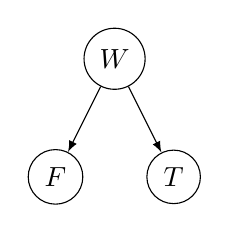
\begin{tikzpicture}[edge from parent/.style={draw,-latex}]
      \node[draw,circle] {$W$}
      child {node[draw,circle] {$F$}}
      child {node[draw,circle] {$T$}};
    \end{tikzpicture}
  \end{subfigure}%
  \begin{subfigure}{0.8\textwidth}
    \centering
    \begin{tabular}[t]{cc}
      \toprule
      $w$ & $\Pr(W = w)$ \\
      \midrule
      1 & 0.5 \\
      0 & 0.5 \\
      \bottomrule
    \end{tabular}
    \begin{tabular}[t]{ccc}
      \toprule
      $w$ & $f$ & $\Pr(F = f \mid W = w)$ \\
      \midrule
      1 & 1 & 0.6 \\
      1 & 0 & 0.4 \\
      0 & 1 & 0.1 \\
      0 & 0 & 0.9 \\
      \bottomrule
    \end{tabular}
    \begin{tabular}[t]{ccc}
      \toprule
      $w$ & $t$ & $\Pr(T = t \mid W = w)$ \\
      \midrule
      1 & $l$ & 0.2 \\
      1 & $m$ & 0.4 \\
      1 & $h$ & 0.4 \\
      0 & $l$ & 0.6 \\
      0 & $m$ & 0.3 \\
      0 & $h$ & 0.1 \\
      \bottomrule
    \end{tabular}
  \end{subfigure}
  \caption{An example Bayesian network with its CPTs}
  \label{fig:example_bn}
\end{figure}

Let $V$ denote the set of random variables in a Bayesian network. For any random
variable $X \in V$, let $\mathrm{pa}(X)$ denote the set of parents of $X$ and
$\im X$ denote the set of possible values. We will use the Bayesian network in
\cref{fig:example_bn} (loosely based on an example by Sang et al.
\cite{DBLP:conf/aaai/SangBK05}) as a running example throughout this section.
For the Bayesian network in \cref{fig:example_bn}, we have:
\begin{align*}
  V &= \{ W, F, T \}, \\
  \mathrm{pa}(W) &= \emptyset, \\
  \mathrm{pa}(F) &= \mathrm{pa}(T) = \{ W \}, \\
  \im W &= \im F = \{ 0, 1 \}, \\
  \im T &= \{ l, m, h \}.
\end{align*}

\begin{definition}[Indicator variables]
  Let $X \in V$ be a random variable. If $X$ is binary (i.e., $|\im X| = 2$), we
  can arbitrary identify one of the values as $1$ and the other one as $0$ (i.e,
  $\im X \cong \{ 0, 1 \}$). Then $X$ can be represented by a single
  \emph{indicator variable} $\lambda_{X=1}$. For notational simplicity, for any
  set $S$, whenever we write $\lambda_{X=0} \in S$ or $S = \{ \lambda_{X=0},
  \dots \}$, we actually mean $\lambda_{X=1} \not\in S$,

  On the other hand, if $X$ is not binary, we represent $X$ with $|\im X|$
  indicator variables, one for each value. We let
  \[
    E(X) = \begin{cases}
      \{ \lambda_{X=1} \} & \text{if } |\im X| = 2 \\
      \{ \lambda_{X=x} \mid x \in \im X \} & \text{otherwise.}
    \end{cases}
  \]
  denote the set of indicator variables for $X$ and
  \[
    E^*(X) = E(X) \cup \bigcup_{Y \in \mathrm{pa}(X)} E(Y).
  \]
  denote the set of indicator variables for $X$ and its parents in the Bayesian
  network. Finally, let
  \[
    U = \bigcup_{X \in V} E(X)
  \]
  denote the set of all indicator variables for all random variables in the
  Bayesian network.
\end{definition}

\todo[inline]{Come up with a less repetitive wording.}
For the Bayesian network in \cref{fig:example_bn}, we have:
\begin{align*}
  E(W) &= \{ \lambda_{W=1} \}, \\
  E(F) &= \{ \lambda_{F=1} \}, \\
  E(T) &= \{ \lambda_{T=l}, \lambda_{T=m}, \lambda_{T=h} \}, \\
  E^*(W) &= \{ \lambda_{W=1} \}, \\
  E^*(F) &= \{ \lambda_{F=1}, \lambda_{W=1} \}, \\
  E^*(T) &= \{ \lambda_{T=l}, \lambda_{T=m}, \lambda_{T=h}, \lambda_{W=1} \}.
\end{align*}

\begin{algorithm}
  \caption{Encoding a Bayesian network as a function $2^U \to \mathbb{R}_{\ge
      0}$}
  \label{alg:encoding}
  \KwData{a Bayesian network with vertices $V$ and probability distribution
    $\Pr$}
  \KwResult{a function $\phi\colon 2^U \to \mathbb{R}_{\ge 0}$}
  $\phi \gets 1$\;
  \For{$X \in V$}{
    \textit{let} $\mathrm{pa}(X) = \{ Y_1, \dots, Y_n \}$\;
    $\mathrm{CPT}_X \gets 0$\;
    \eIf{$|\im X| = 2$}{
      \For{$(y_1, \dots, y_n) \in \prod_{i = 1}^n \im Y_i$}{
        $p_1 \gets \Pr(X = 1 \mid Y_1 = y_1, \dots, Y_n = y_n)$\;
        $p_0 \gets \Pr(X \ne 1 \mid Y_1 = y_1, \dots, Y_n = y_n)$\;
        $\mathrm{CPT}_X \gets \mathrm{CPT}_X + p_1[\lambda_{X=1}] \cdot
        \prod_{i=1}^n [\lambda_{Y_i=y_i}] + p_0 \overline{[\lambda_{X=1}]} \cdot
        \prod_{i=1}^n [\lambda_{Y_i=y_i}]$\;
      }
    }{
      \textit{let} $\im X = \{ x_1, \dots, x_m \}$\;
      \For{$x \in \im X$ {\rm \textbf{and}} $(y_1, \dots, y_n) \in \prod_{i =
          1}^n \im Y_i$}{
        $p_x \gets \Pr(X = x \mid Y_1 = y_1, \dots, Y_n = y_n)$\;
        $\mathrm{CPT}_X \gets \mathrm{CPT}_X + p_x[\lambda_{X=x}] \cdot
        \prod_{i=1}^n [\lambda_{Y_i=y_i}] + \overline{[\lambda_{X=1}]} \cdot
        \prod_{i=1}^n [\lambda_{Y_i=y_i}]$\;
      }
      $\mathrm{CPT}_X \gets \mathrm{CPT}_X \cdot \left( \sum_{i=1}^m [\lambda_{X
          = x_i}] \right) \cdot \prod_{i=1}^m \prod_{j=i+1}^m
      (\overline{[\lambda_{X = x_i}]} + \overline{[\lambda_{X = x_j}]})$\;
    }
    $\phi \gets \phi \cdot \mathrm{CPT}_X$\;
  }
  \Return{$\phi$}\;
\end{algorithm}

\todo[inline]{Ditto.}
For the Bayesian network in \cref{fig:example_bn}, we have:
\begin{align*}
  \mathrm{CPT_W} &= 0.5[\lambda_{W=1}]+0.5\overline{[\lambda_{W=1}]} = 0.5 \cdot 1, \\
  \mathrm{CPT_F} &= 0.6[\lambda_{F=1}] \cdot [\lambda_{W=1}] + 0.4[\lambda_{F=0}] \cdot [\lambda_{W=1}] + 0.1[\lambda_{F=1}] \cdot [\lambda_{W=0}] + 0.9[\lambda_{F=0}] \cdot [\lambda_{W=0}] \\
    &= 0.6[\lambda_{F=1}] \cdot [\lambda_{W=1}] + 0.4\overline{[\lambda_{F=1}]} \cdot [\lambda_{W=1}] + 0.1[\lambda_{F=1}] \cdot \overline{[\lambda_{W=1}]} + 0.9\overline{[\lambda_{F=1}]} \cdot \overline{[\lambda_{W=1}]}, \\
  \mathrm{CPT_T} &= ([\lambda_{T=l}] + [\lambda_{T=m}] + [\lambda_{T=h}]) \cdot (\overline{[\lambda_{T=l}]} + \overline{[\lambda_{T=m}]}) \cdot (\overline{[\lambda_{T=l}]} + \overline{[\lambda_{T=h}]}) \cdot (\overline{[\lambda_{T=m}]} + \overline{[\lambda_{T=h}]}) \cdot (\dots).
\end{align*}

\todo[inline]{Describe \cref{alg:encoding}}

\subsection{Proof of Correctness}

\begin{lemma} \label{lemma:cpt}
  Let $X \in V$ be a random variable with parents $\mathrm{pa}(X) = \{ Y_1,
  \dots, Y_n \}$. Then $\mathrm{CPT}_X\colon 2^{E^*(X)} \to \mathbb{R}_{\ge 0}$
  is such that for any $x \in \im X$ and $(y_1, \dots, y_n) \in \prod_{i=1}^n
  \im Y_i$,
  \[
    \mathrm{CPT}_X (\{ \lambda_{X=x} \} \cup \{ \lambda_{Y_i=y_i} \mid i = 1,
    \dots, n \}) = \Pr(X = x \mid Y_1 = y_1, \dots, Y_n = y_n).
  \]
\end{lemma}
\begin{proof}
  Let $\tau = \{ \lambda_{X=x} \} \cup \{ \lambda_{Y_i=y_i} \mid i = 1, \dots, n
  \}$. If $X$ is binary, then $\mathrm{CPT}_X$ is a sum of $2\prod_{i=1}^n |\im
  Y_i|$ terms, one for each possible assignment of values to variables $X, Y_1,
  \dots, Y_n$. Exactly one of these terms is nonzero when applied to $\tau$, and
  it is equal to $\Pr(X = x \mid Y_1 = y_1, \dots, Y_n = y_n)$ by definition.

  If $X$ is not binary, then
  \[
    \left( \sum_{i=1}^m [\lambda_{X = x_i}] \right)(\tau) = 1,
  \]
  and
  \[
    \left( \prod_{i=1}^m \prod_{j=i+1}^m (\overline{[\lambda_{X = x_i}]} +
      \overline{[\lambda_{X = x_j}]}) \right)(\tau) = 1,
  \]
  so, by a similar argument as before,
  \[
    \mathrm{CPT}_X(\tau) = \Pr(X = x \mid Y_1 = y_1, \dots, Y_n = y_n).
  \]
\end{proof}

\begin{proposition} \label{lemma:full_distribution}
  $\phi\colon 2^U \to \mathbb{R}_{\ge 0}$ represents the full probability
  distribution of the Bayesian network, i.e., if $V = \{ X_1, \dots, X_n\}$,
  then
  \[
    \phi(\tau) =
    \begin{cases}
      \Pr(X_1 = x_1, \dots, X_n = x_n) & \text{if } \tau = \{ \lambda_{X_i=x_i}
      \mid i = 1, \dots, n \} \text{ for some } (x_1, \dots, x_n) \in
      \prod_{i=1}^n \im X_i \\
      0 & \text{otherwise,}
    \end{cases}
  \]
  for all $\tau \in 2^U$.
\end{proposition}
\begin{proof}
  If $\tau = \{ \lambda_{X=v_X} \mid X \in V \}$ for some $(v_X)_{X \in V} \in
  \prod_{X \in V} \im X$, then
  \[
    \phi(\tau) = \prod_{X \in V} \Pr \left( X=v_X \;\middle|\; \bigwedge_{Y \in
        \mathrm{pa}(X)} Y=v_Y \right) = \Pr \left( \bigwedge_{X \in V} X=v_X
    \right)
  \]
  by \cref{lemma:cpt} and the definition of a Bayesian network. Otherwise there
  must be some non-binary random variable $X \in V$ such that $|E(X) \cap \tau|
  \ne 1$. If $E(X) \cap \tau = \emptyset$, then
  \[
    \left( \sum_{i=1}^m [\lambda_{X = x_i}] \right)(\tau) = 0,
  \]
  and so $\mathrm{CPT}_X(\tau) = 0$, and $\phi(\tau) = 0$. If $|E(X) \cap
  \tau| > 1$, then we must have two different values $x_1, x_2 \in \im X$ such
  that $\{\lambda_{X=x_1}, \lambda_{X=x_2} \} \subseteq \tau$ which means that
  \[
    (\overline{[\lambda_{X=x_1}]} + \overline{[\lambda_{X=x_2}]})(\tau) = 0,
  \]
  and so, again, $\mathrm{CPT}_X(\tau) = 0$, and $\phi(\tau) = 0$.
\end{proof}

\begin{theorem}
  Let $\phi\colon 2^U \to \mathbb{R}_{\ge 0}$ be a function generated by the
  algorithm. Then
  \[
    (\exists_U(\phi \cdot [\lambda_{X=x}]))(\emptyset) = \Pr(X = x).
  \]
\end{theorem}
\begin{proof}
  Let $V = \{ X, Y_1, \dots, Y_n \}$. Then
  \begin{align*}
    (\exists_U (\phi \cdot [\lambda_{X=x}]))(\emptyset) &= \sum_{\tau \in 2^U} (\phi \cdot [\lambda_{X=x}])(\tau) = \sum_{\lambda_{X=x} \in \tau \in 2^U} \phi(\tau) = \sum_{\lambda_{X=x} \in \tau \in 2^U} \left( \prod_{Y \in V} \mathrm{CPT}_Y \right)(\tau) \\
    &= \sum_{(y_1, \dots, y_n) \in \prod_{i=1}^n \im Y_i} \Pr(X = x, Y_1 = y_1, \dots, Y_n = y_n) = \Pr(X = x)
  \end{align*}
  by the following arguments:
  \begin{itemize}
  \item the proof of Theorem~1 in the ADDMC paper \cite{DBLP:conf/aaai/DudekPV20};
  \item if $\lambda_{X=x} \not\in \tau \in 2^U$, then $(\phi \cdot
    [\lambda_{X=x}])(\tau) = \phi(\tau) \cdot [\lambda_{X=x}](\tau \cap \{
    \lambda_{X=x} \}) = \phi(\tau) \cdot 0 = 0$;
  \item \cref{lemma:full_distribution};
  \item marginalisation of a probability distribution.
  \end{itemize}
\end{proof}

\subsection{Textual Representation}

The Bayesian network in \cref{fig:example_bn} can be represented in a textual
format as
\[
  \begin{array}{l r r l l}
    \lambda\sb{T=l} &\lambda\sb{T=m} &\lambda\sb{T=h} & &0 \\
                    &-\lambda\sb{T=l} &-\lambda\sb{T=m} & &0 \\
                    &-\lambda\sb{T=l} &-\lambda\sb{T=h} & &0 \\
                    &-\lambda\sb{T=m} &-\lambda\sb{T=h} & &0 \\
    w &\lambda\sb{W=1} & &0.5 &0.5 \\
    w &\lambda\sb{F=1} &\lambda\sb{W=1} &0.6 &0.4 \\
    w &\lambda\sb{F=1} &-\lambda\sb{W=1} &0.1 &0.9 \\
    w &\lambda\sb{T=l} &\lambda\sb{W=1} &0.2 &1 \\
    w &\lambda\sb{T=m} &\lambda\sb{W=1} &0.4 &1 \\
    w &\lambda\sb{T=h} &\lambda\sb{W=1} &0.4 &1 \\
    w &\lambda\sb{T=l} &\lambda\sb{W=0} &0.6 &1 \\
    w &\lambda\sb{T=m} &\lambda\sb{W=0} &0.3 &1 \\
    w &\lambda\sb{T=h} &\lambda\sb{W=0} &0.1 &1
  \end{array}
\]
with each $\lambda$ replaced with a unique positive integer. This format is
based on the format used by the Cachet solver \cite{DBLP:conf/sat/SangBBKP04}
to encode WMC problems, which extends the DIMACS format for CNF formulas with
weight clauses. Subsequently, we extend it in two ways:
\begin{itemize}
\item a single weight clause now supports an arbitrary number of literals,
\item and each weight clause has two probabilities instead of one (i.e., we no
  longer assume that $\Pr(v) + \Pr(\neg v) = 1$ for all variables $v \in U$).
\end{itemize}
The way we use this encoding, it is always the case that either both
probabilities sum to one, or the second probability (i.e., the probability for
the complement of the variable) is equal to one.

\subsection{Changes to ADDMC}

ADDMC constructs the \emph{Gaifman graph} \cite{gaifman1982local} of the input
CNF formula as an aid for the algorithm's heuristics. This graph has as vertices
the variables of the formula, and there is an edge between two variables $u$ and
$v$ if there is a clause in the formula that contains both $u$ and $v$. We
extend this definition to functions on Boolean algebras, i.e., the factors of
$\phi$. For any pair of distinct variables $u, v \in U$, we draw an edge between
them in the Gaifman graph if there is a function $A\colon 2^X \to
\mathbb{R}_{\ge 0}$ that is a factor of $\phi$ such that $u \in X$ and $v \in
X$. For instance, a factor such as $\mathrm{CPT}_X$ will enable edges between
all distinct pairs of variables in $E^*(X)$.

\todo[inline]{This needs rewriting.}
ADDMC multiplies the final answer by $w(u)+w(-u)$ for every $u \in U$ that was
`simplified out' of the ADD for $\phi$ and so is not featured in the $\exists_U$
projection. In our format, for every such $u \in U$, we multiply the answer by
two. Each such $u \in U$ must satisfy two properties:
\begin{itemize}
\item all the probabilities/weights associated with $u$ are equal to $0.5$
  (otherwise the corresponding CPT would depend on $u$),
\item and all other CPTs are independent of $u$ (or they may have a trivial
  dependence, where the probability stays the same if $u$ is replaced with its
  complement).
\end{itemize}
Thus, the CPT that corresponds to $u$ still multiplies every model by $0.5$, but
the number of models being considered by the ADDMC is halved. To correct for
this, we need to perform this multiplication.

\section{Experimental Comparison} \label{sec:experiments}

\begin{figure}
  \centering
  % Created by tikzDevice version 0.12.3 on 2020-07-28 14:07:53
% !TEX encoding = UTF-8 Unicode
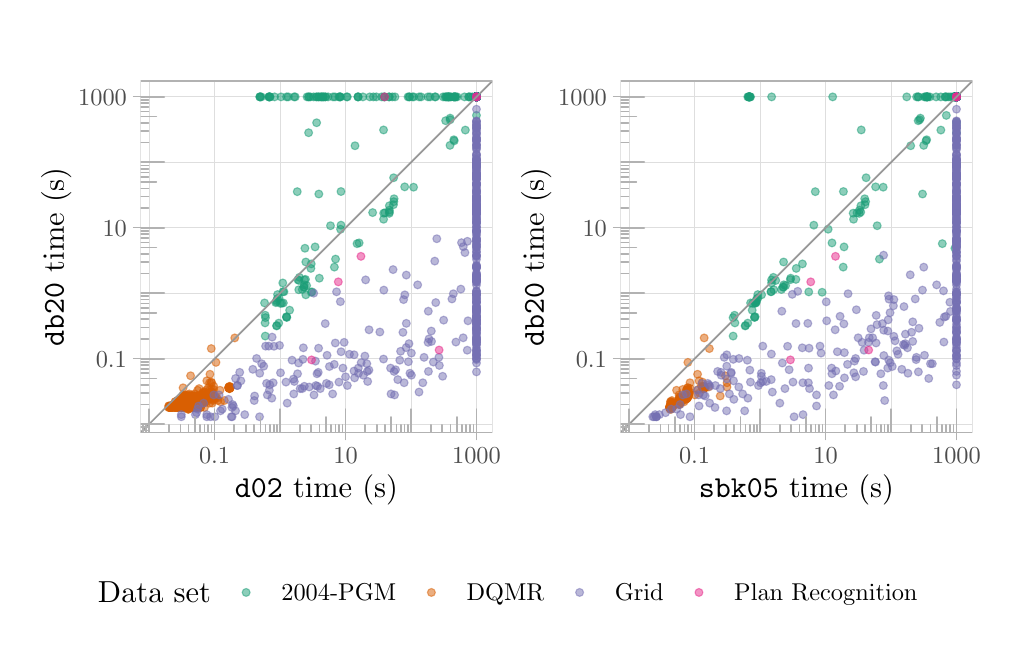
\begin{tikzpicture}[x=1pt,y=1pt]
\definecolor{fillColor}{RGB}{255,255,255}
\path[use as bounding box,fill=fillColor,fill opacity=0.00] (0,0) rectangle (346.90,216.81);
\begin{scope}
\path[clip] (  0.00, 39.18) rectangle (173.45,203.08);
\definecolor{drawColor}{RGB}{255,255,255}
\definecolor{fillColor}{RGB}{255,255,255}

\path[draw=drawColor,line width= 0.6pt,line join=round,line cap=round,fill=fillColor] (  0.00, 39.18) rectangle (173.45,203.08);
\end{scope}
\begin{scope}
\path[clip] ( 40.80, 70.44) rectangle (167.95,197.58);
\definecolor{fillColor}{RGB}{255,255,255}

\path[fill=fillColor] ( 40.80, 70.44) rectangle (167.95,197.58);
\definecolor{drawColor}{gray}{0.87}

\path[draw=drawColor,line width= 0.1pt,line join=round] ( 40.80, 73.52) --
	(167.95, 73.52);

\path[draw=drawColor,line width= 0.1pt,line join=round] ( 40.80,120.83) --
	(167.95,120.83);

\path[draw=drawColor,line width= 0.1pt,line join=round] ( 40.80,168.15) --
	(167.95,168.15);

\path[draw=drawColor,line width= 0.1pt,line join=round] ( 43.88, 70.44) --
	( 43.88,197.58);

\path[draw=drawColor,line width= 0.1pt,line join=round] ( 91.20, 70.44) --
	( 91.20,197.58);

\path[draw=drawColor,line width= 0.1pt,line join=round] (138.51, 70.44) --
	(138.51,197.58);

\path[draw=drawColor,line width= 0.3pt,line join=round] ( 40.80, 97.18) --
	(167.95, 97.18);

\path[draw=drawColor,line width= 0.3pt,line join=round] ( 40.80,144.49) --
	(167.95,144.49);

\path[draw=drawColor,line width= 0.3pt,line join=round] ( 40.80,191.80) --
	(167.95,191.80);

\path[draw=drawColor,line width= 0.3pt,line join=round] ( 67.54, 70.44) --
	( 67.54,197.58);

\path[draw=drawColor,line width= 0.3pt,line join=round] (114.86, 70.44) --
	(114.86,197.58);

\path[draw=drawColor,line width= 0.3pt,line join=round] (162.17, 70.44) --
	(162.17,197.58);
\definecolor{drawColor}{RGB}{27,158,119}
\definecolor{fillColor}{RGB}{27,158,119}

\path[draw=drawColor,draw opacity=0.50,line width= 0.4pt,line join=round,line cap=round,fill=fillColor,fill opacity=0.50] ( 87.58,191.80) circle (  1.43);

\path[draw=drawColor,draw opacity=0.50,line width= 0.4pt,line join=round,line cap=round,fill=fillColor,fill opacity=0.50] ( 87.16,191.80) circle (  1.43);

\path[draw=drawColor,draw opacity=0.50,line width= 0.4pt,line join=round,line cap=round,fill=fillColor,fill opacity=0.50] ( 87.36,191.80) circle (  1.43);

\path[draw=drawColor,draw opacity=0.50,line width= 0.4pt,line join=round,line cap=round,fill=fillColor,fill opacity=0.50] ( 89.22,191.80) circle (  1.43);

\path[draw=drawColor,draw opacity=0.50,line width= 0.4pt,line join=round,line cap=round,fill=fillColor,fill opacity=0.50] ( 87.16,191.80) circle (  1.43);

\path[draw=drawColor,draw opacity=0.50,line width= 0.4pt,line join=round,line cap=round,fill=fillColor,fill opacity=0.50] ( 87.53,191.80) circle (  1.43);

\path[draw=drawColor,draw opacity=0.50,line width= 0.4pt,line join=round,line cap=round,fill=fillColor,fill opacity=0.50] ( 85.83,112.90) circle (  1.43);

\path[draw=drawColor,draw opacity=0.50,line width= 0.4pt,line join=round,line cap=round,fill=fillColor,fill opacity=0.50] ( 85.93,112.04) circle (  1.43);

\path[draw=drawColor,draw opacity=0.50,line width= 0.4pt,line join=round,line cap=round,fill=fillColor,fill opacity=0.50] ( 85.85,105.37) circle (  1.43);

\path[draw=drawColor,draw opacity=0.50,line width= 0.4pt,line join=round,line cap=round,fill=fillColor,fill opacity=0.50] ( 94.66,114.73) circle (  1.43);

\path[draw=drawColor,draw opacity=0.50,line width= 0.4pt,line join=round,line cap=round,fill=fillColor,fill opacity=0.50] ( 85.79,110.13) circle (  1.43);

\path[draw=drawColor,draw opacity=0.50,line width= 0.4pt,line join=round,line cap=round,fill=fillColor,fill opacity=0.50] ( 84.44,191.80) circle (  1.43);

\path[draw=drawColor,draw opacity=0.50,line width= 0.4pt,line join=round,line cap=round,fill=fillColor,fill opacity=0.50] ( 83.89,191.80) circle (  1.43);

\path[draw=drawColor,draw opacity=0.50,line width= 0.4pt,line join=round,line cap=round,fill=fillColor,fill opacity=0.50] ( 94.17,191.80) circle (  1.43);

\path[draw=drawColor,draw opacity=0.50,line width= 0.4pt,line join=round,line cap=round,fill=fillColor,fill opacity=0.50] ( 83.95,191.80) circle (  1.43);

\path[draw=drawColor,draw opacity=0.50,line width= 0.4pt,line join=round,line cap=round,fill=fillColor,fill opacity=0.50] ( 83.99,191.80) circle (  1.43);

\path[draw=drawColor,draw opacity=0.50,line width= 0.4pt,line join=round,line cap=round,fill=fillColor,fill opacity=0.50] ( 90.30,120.37) circle (  1.43);

\path[draw=drawColor,draw opacity=0.50,line width= 0.4pt,line join=round,line cap=round,fill=fillColor,fill opacity=0.50] ( 89.65,117.47) circle (  1.43);

\path[draw=drawColor,draw opacity=0.50,line width= 0.4pt,line join=round,line cap=round,fill=fillColor,fill opacity=0.50] ( 90.00,118.21) circle (  1.43);

\path[draw=drawColor,draw opacity=0.50,line width= 0.4pt,line join=round,line cap=round,fill=fillColor,fill opacity=0.50] ( 98.04,125.45) circle (  1.43);

\path[draw=drawColor,draw opacity=0.50,line width= 0.4pt,line join=round,line cap=round,fill=fillColor,fill opacity=0.50] ( 89.93,117.73) circle (  1.43);

\path[draw=drawColor,draw opacity=0.50,line width= 0.4pt,line join=round,line cap=round,fill=fillColor,fill opacity=0.50] ( 90.82,119.15) circle (  1.43);

\path[draw=drawColor,draw opacity=0.50,line width= 0.4pt,line join=round,line cap=round,fill=fillColor,fill opacity=0.50] (100.51,120.28) circle (  1.43);

\path[draw=drawColor,draw opacity=0.50,line width= 0.4pt,line join=round,line cap=round,fill=fillColor,fill opacity=0.50] ( 90.02,109.16) circle (  1.43);

\path[draw=drawColor,draw opacity=0.50,line width= 0.4pt,line join=round,line cap=round,fill=fillColor,fill opacity=0.50] ( 90.73,110.05) circle (  1.43);

\path[draw=drawColor,draw opacity=0.50,line width= 0.4pt,line join=round,line cap=round,fill=fillColor,fill opacity=0.50] ( 89.94,109.03) circle (  1.43);

\path[draw=drawColor,draw opacity=0.50,line width= 0.4pt,line join=round,line cap=round,fill=fillColor,fill opacity=0.50] ( 85.60,117.34) circle (  1.43);

\path[draw=drawColor,draw opacity=0.50,line width= 0.4pt,line join=round,line cap=round,fill=fillColor,fill opacity=0.50] ( 92.38,117.34) circle (  1.43);

\path[draw=drawColor,draw opacity=0.50,line width= 0.4pt,line join=round,line cap=round,fill=fillColor,fill opacity=0.50] ( 99.98,125.66) circle (  1.43);

\path[draw=drawColor,draw opacity=0.50,line width= 0.4pt,line join=round,line cap=round,fill=fillColor,fill opacity=0.50] ( 91.83,117.27) circle (  1.43);

\path[draw=drawColor,draw opacity=0.50,line width= 0.4pt,line join=round,line cap=round,fill=fillColor,fill opacity=0.50] ( 98.21,126.59) circle (  1.43);

\path[draw=drawColor,draw opacity=0.50,line width= 0.4pt,line join=round,line cap=round,fill=fillColor,fill opacity=0.50] ( 91.33,117.18) circle (  1.43);

\path[draw=drawColor,draw opacity=0.50,line width= 0.4pt,line join=round,line cap=round,fill=fillColor,fill opacity=0.50] ( 99.91,123.05) circle (  1.43);

\path[draw=drawColor,draw opacity=0.50,line width= 0.4pt,line join=round,line cap=round,fill=fillColor,fill opacity=0.50] ( 99.78,123.06) circle (  1.43);

\path[draw=drawColor,draw opacity=0.50,line width= 0.4pt,line join=round,line cap=round,fill=fillColor,fill opacity=0.50] (102.47,131.45) circle (  1.43);

\path[draw=drawColor,draw opacity=0.50,line width= 0.4pt,line join=round,line cap=round,fill=fillColor,fill opacity=0.50] ( 99.24,122.20) circle (  1.43);

\path[draw=drawColor,draw opacity=0.50,line width= 0.4pt,line join=round,line cap=round,fill=fillColor,fill opacity=0.50] ( 99.95,123.90) circle (  1.43);

\path[draw=drawColor,draw opacity=0.50,line width= 0.4pt,line join=round,line cap=round,fill=fillColor,fill opacity=0.50] (100.80,123.61) circle (  1.43);

\path[draw=drawColor,draw opacity=0.50,line width= 0.4pt,line join=round,line cap=round,fill=fillColor,fill opacity=0.50] ( 93.53,112.23) circle (  1.43);

\path[draw=drawColor,draw opacity=0.50,line width= 0.4pt,line join=round,line cap=round,fill=fillColor,fill opacity=0.50] ( 90.21,118.87) circle (  1.43);

\path[draw=drawColor,draw opacity=0.50,line width= 0.4pt,line join=round,line cap=round,fill=fillColor,fill opacity=0.50] (105.39,126.28) circle (  1.43);

\path[draw=drawColor,draw opacity=0.50,line width= 0.4pt,line join=round,line cap=round,fill=fillColor,fill opacity=0.50] ( 93.52,112.37) circle (  1.43);

\path[draw=drawColor,draw opacity=0.50,line width= 0.4pt,line join=round,line cap=round,fill=fillColor,fill opacity=0.50] ( 93.63,112.09) circle (  1.43);

\path[draw=drawColor,draw opacity=0.50,line width= 0.4pt,line join=round,line cap=round,fill=fillColor,fill opacity=0.50] (102.33,129.82) circle (  1.43);

\path[draw=drawColor,draw opacity=0.50,line width= 0.4pt,line join=round,line cap=round,fill=fillColor,fill opacity=0.50] ( 92.25,121.42) circle (  1.43);

\path[draw=drawColor,draw opacity=0.50,line width= 0.4pt,line join=round,line cap=round,fill=fillColor,fill opacity=0.50] ( 92.61,121.38) circle (  1.43);

\path[draw=drawColor,draw opacity=0.50,line width= 0.4pt,line join=round,line cap=round,fill=fillColor,fill opacity=0.50] ( 92.18,124.56) circle (  1.43);

\path[draw=drawColor,draw opacity=0.50,line width= 0.4pt,line join=round,line cap=round,fill=fillColor,fill opacity=0.50] ( 97.96,122.11) circle (  1.43);

\path[draw=drawColor,draw opacity=0.50,line width= 0.4pt,line join=round,line cap=round,fill=fillColor,fill opacity=0.50] (162.17,191.80) circle (  1.43);

\path[draw=drawColor,draw opacity=0.50,line width= 0.4pt,line join=round,line cap=round,fill=fillColor,fill opacity=0.50] (128.98,191.80) circle (  1.43);

\path[draw=drawColor,draw opacity=0.50,line width= 0.4pt,line join=round,line cap=round,fill=fillColor,fill opacity=0.50] (137.43,191.80) circle (  1.43);

\path[draw=drawColor,draw opacity=0.50,line width= 0.4pt,line join=round,line cap=round,fill=fillColor,fill opacity=0.50] (162.17,191.80) circle (  1.43);

\path[draw=drawColor,draw opacity=0.50,line width= 0.4pt,line join=round,line cap=round,fill=fillColor,fill opacity=0.50] (128.80,191.80) circle (  1.43);

\path[draw=drawColor,draw opacity=0.50,line width= 0.4pt,line join=round,line cap=round,fill=fillColor,fill opacity=0.50] (162.17,191.80) circle (  1.43);

\path[draw=drawColor,draw opacity=0.50,line width= 0.4pt,line join=round,line cap=round,fill=fillColor,fill opacity=0.50] (128.60,179.85) circle (  1.43);

\path[draw=drawColor,draw opacity=0.50,line width= 0.4pt,line join=round,line cap=round,fill=fillColor,fill opacity=0.50] (136.23,159.29) circle (  1.43);

\path[draw=drawColor,draw opacity=0.50,line width= 0.4pt,line join=round,line cap=round,fill=fillColor,fill opacity=0.50] (128.60,147.58) circle (  1.43);

\path[draw=drawColor,draw opacity=0.50,line width= 0.4pt,line join=round,line cap=round,fill=fillColor,fill opacity=0.50] (129.11,149.92) circle (  1.43);

\path[draw=drawColor,draw opacity=0.50,line width= 0.4pt,line join=round,line cap=round,fill=fillColor,fill opacity=0.50] (128.65,149.77) circle (  1.43);

\path[draw=drawColor,draw opacity=0.50,line width= 0.4pt,line join=round,line cap=round,fill=fillColor,fill opacity=0.50] (147.37,191.80) circle (  1.43);

\path[draw=drawColor,draw opacity=0.50,line width= 0.4pt,line join=round,line cap=round,fill=fillColor,fill opacity=0.50] (162.17,191.80) circle (  1.43);

\path[draw=drawColor,draw opacity=0.50,line width= 0.4pt,line join=round,line cap=round,fill=fillColor,fill opacity=0.50] (141.45,191.80) circle (  1.43);

\path[draw=drawColor,draw opacity=0.50,line width= 0.4pt,line join=round,line cap=round,fill=fillColor,fill opacity=0.50] (152.49,191.80) circle (  1.43);

\path[draw=drawColor,draw opacity=0.50,line width= 0.4pt,line join=round,line cap=round,fill=fillColor,fill opacity=0.50] (145.40,191.80) circle (  1.43);

\path[draw=drawColor,draw opacity=0.50,line width= 0.4pt,line join=round,line cap=round,fill=fillColor,fill opacity=0.50] (162.17,191.80) circle (  1.43);

\path[draw=drawColor,draw opacity=0.50,line width= 0.4pt,line join=round,line cap=round,fill=fillColor,fill opacity=0.50] (139.52,191.80) circle (  1.43);

\path[draw=drawColor,draw opacity=0.50,line width= 0.4pt,line join=round,line cap=round,fill=fillColor,fill opacity=0.50] (130.51,191.80) circle (  1.43);

\path[draw=drawColor,draw opacity=0.50,line width= 0.4pt,line join=round,line cap=round,fill=fillColor,fill opacity=0.50] (162.17,191.80) circle (  1.43);

\path[draw=drawColor,draw opacity=0.50,line width= 0.4pt,line join=round,line cap=round,fill=fillColor,fill opacity=0.50] (162.17,191.80) circle (  1.43);

\path[draw=drawColor,draw opacity=0.50,line width= 0.4pt,line join=round,line cap=round,fill=fillColor,fill opacity=0.50] (162.17,191.80) circle (  1.43);

\path[draw=drawColor,draw opacity=0.50,line width= 0.4pt,line join=round,line cap=round,fill=fillColor,fill opacity=0.50] (139.44,159.17) circle (  1.43);

\path[draw=drawColor,draw opacity=0.50,line width= 0.4pt,line join=round,line cap=round,fill=fillColor,fill opacity=0.50] (130.69,150.87) circle (  1.43);

\path[draw=drawColor,draw opacity=0.50,line width= 0.4pt,line join=round,line cap=round,fill=fillColor,fill opacity=0.50] (130.73,150.19) circle (  1.43);

\path[draw=drawColor,draw opacity=0.50,line width= 0.4pt,line join=round,line cap=round,fill=fillColor,fill opacity=0.50] (130.70,152.45) circle (  1.43);

\path[draw=drawColor,draw opacity=0.50,line width= 0.4pt,line join=round,line cap=round,fill=fillColor,fill opacity=0.50] (130.66,149.71) circle (  1.43);

\path[draw=drawColor,draw opacity=0.50,line width= 0.4pt,line join=round,line cap=round,fill=fillColor,fill opacity=0.50] (162.17,191.80) circle (  1.43);

\path[draw=drawColor,draw opacity=0.50,line width= 0.4pt,line join=round,line cap=round,fill=fillColor,fill opacity=0.50] (159.94,191.80) circle (  1.43);

\path[draw=drawColor,draw opacity=0.50,line width= 0.4pt,line join=round,line cap=round,fill=fillColor,fill opacity=0.50] (142.16,191.80) circle (  1.43);

\path[draw=drawColor,draw opacity=0.50,line width= 0.4pt,line join=round,line cap=round,fill=fillColor,fill opacity=0.50] (159.50,191.80) circle (  1.43);

\path[draw=drawColor,draw opacity=0.50,line width= 0.4pt,line join=round,line cap=round,fill=fillColor,fill opacity=0.50] (157.85,191.80) circle (  1.43);

\path[draw=drawColor,draw opacity=0.50,line width= 0.4pt,line join=round,line cap=round,fill=fillColor,fill opacity=0.50] (162.17,191.80) circle (  1.43);

\path[draw=drawColor,draw opacity=0.50,line width= 0.4pt,line join=round,line cap=round,fill=fillColor,fill opacity=0.50] (162.17,191.80) circle (  1.43);

\path[draw=drawColor,draw opacity=0.50,line width= 0.4pt,line join=round,line cap=round,fill=fillColor,fill opacity=0.50] (162.17,191.80) circle (  1.43);

\path[draw=drawColor,draw opacity=0.50,line width= 0.4pt,line join=round,line cap=round,fill=fillColor,fill opacity=0.50] (162.17,191.80) circle (  1.43);

\path[draw=drawColor,draw opacity=0.50,line width= 0.4pt,line join=round,line cap=round,fill=fillColor,fill opacity=0.50] (162.17,191.80) circle (  1.43);

\path[draw=drawColor,draw opacity=0.50,line width= 0.4pt,line join=round,line cap=round,fill=fillColor,fill opacity=0.50] (162.17,191.80) circle (  1.43);

\path[draw=drawColor,draw opacity=0.50,line width= 0.4pt,line join=round,line cap=round,fill=fillColor,fill opacity=0.50] (162.17,191.80) circle (  1.43);

\path[draw=drawColor,draw opacity=0.50,line width= 0.4pt,line join=round,line cap=round,fill=fillColor,fill opacity=0.50] (132.39,154.99) circle (  1.43);

\path[draw=drawColor,draw opacity=0.50,line width= 0.4pt,line join=round,line cap=round,fill=fillColor,fill opacity=0.50] (132.23,162.58) circle (  1.43);

\path[draw=drawColor,draw opacity=0.50,line width= 0.4pt,line join=round,line cap=round,fill=fillColor,fill opacity=0.50] (132.30,153.93) circle (  1.43);

\path[draw=drawColor,draw opacity=0.50,line width= 0.4pt,line join=round,line cap=round,fill=fillColor,fill opacity=0.50] (132.16,152.83) circle (  1.43);

\path[draw=drawColor,draw opacity=0.50,line width= 0.4pt,line join=round,line cap=round,fill=fillColor,fill opacity=0.50] (162.17,191.80) circle (  1.43);

\path[draw=drawColor,draw opacity=0.50,line width= 0.4pt,line join=round,line cap=round,fill=fillColor,fill opacity=0.50] (162.17,191.80) circle (  1.43);

\path[draw=drawColor,draw opacity=0.50,line width= 0.4pt,line join=round,line cap=round,fill=fillColor,fill opacity=0.50] (162.17,191.80) circle (  1.43);

\path[draw=drawColor,draw opacity=0.50,line width= 0.4pt,line join=round,line cap=round,fill=fillColor,fill opacity=0.50] (162.03,191.80) circle (  1.43);

\path[draw=drawColor,draw opacity=0.50,line width= 0.4pt,line join=round,line cap=round,fill=fillColor,fill opacity=0.50] (162.17,191.80) circle (  1.43);

\path[draw=drawColor,draw opacity=0.50,line width= 0.4pt,line join=round,line cap=round,fill=fillColor,fill opacity=0.50] (162.17,191.80) circle (  1.43);

\path[draw=drawColor,draw opacity=0.50,line width= 0.4pt,line join=round,line cap=round,fill=fillColor,fill opacity=0.50] (161.96,191.80) circle (  1.43);

\path[draw=drawColor,draw opacity=0.50,line width= 0.4pt,line join=round,line cap=round,fill=fillColor,fill opacity=0.50] (162.12,191.80) circle (  1.43);

\path[draw=drawColor,draw opacity=0.50,line width= 0.4pt,line join=round,line cap=round,fill=fillColor,fill opacity=0.50] (162.17,191.80) circle (  1.43);

\path[draw=drawColor,draw opacity=0.50,line width= 0.4pt,line join=round,line cap=round,fill=fillColor,fill opacity=0.50] (162.06,191.80) circle (  1.43);

\path[draw=drawColor,draw opacity=0.50,line width= 0.4pt,line join=round,line cap=round,fill=fillColor,fill opacity=0.50] (162.17,191.80) circle (  1.43);

\path[draw=drawColor,draw opacity=0.50,line width= 0.4pt,line join=round,line cap=round,fill=fillColor,fill opacity=0.50] (151.21,191.80) circle (  1.43);

\path[draw=drawColor,draw opacity=0.50,line width= 0.4pt,line join=round,line cap=round,fill=fillColor,fill opacity=0.50] (151.03,183.19) circle (  1.43);

\path[draw=drawColor,draw opacity=0.50,line width= 0.4pt,line join=round,line cap=round,fill=fillColor,fill opacity=0.50] (151.34,191.80) circle (  1.43);

\path[draw=drawColor,draw opacity=0.50,line width= 0.4pt,line join=round,line cap=round,fill=fillColor,fill opacity=0.50] (147.15,191.80) circle (  1.43);

\path[draw=drawColor,draw opacity=0.50,line width= 0.4pt,line join=round,line cap=round,fill=fillColor,fill opacity=0.50] (160.77,191.80) circle (  1.43);

\path[draw=drawColor,draw opacity=0.50,line width= 0.4pt,line join=round,line cap=round,fill=fillColor,fill opacity=0.50] (152.57,191.80) circle (  1.43);

\path[draw=drawColor,draw opacity=0.50,line width= 0.4pt,line join=round,line cap=round,fill=fillColor,fill opacity=0.50] (162.17,191.80) circle (  1.43);

\path[draw=drawColor,draw opacity=0.50,line width= 0.4pt,line join=round,line cap=round,fill=fillColor,fill opacity=0.50] (154.41,191.80) circle (  1.43);

\path[draw=drawColor,draw opacity=0.50,line width= 0.4pt,line join=round,line cap=round,fill=fillColor,fill opacity=0.50] (159.35,191.80) circle (  1.43);

\path[draw=drawColor,draw opacity=0.50,line width= 0.4pt,line join=round,line cap=round,fill=fillColor,fill opacity=0.50] (154.58,191.80) circle (  1.43);

\path[draw=drawColor,draw opacity=0.50,line width= 0.4pt,line join=round,line cap=round,fill=fillColor,fill opacity=0.50] (162.17,191.80) circle (  1.43);

\path[draw=drawColor,draw opacity=0.50,line width= 0.4pt,line join=round,line cap=round,fill=fillColor,fill opacity=0.50] (162.17,191.80) circle (  1.43);

\path[draw=drawColor,draw opacity=0.50,line width= 0.4pt,line join=round,line cap=round,fill=fillColor,fill opacity=0.50] (162.17,191.80) circle (  1.43);

\path[draw=drawColor,draw opacity=0.50,line width= 0.4pt,line join=round,line cap=round,fill=fillColor,fill opacity=0.50] (162.17,191.80) circle (  1.43);

\path[draw=drawColor,draw opacity=0.50,line width= 0.4pt,line join=round,line cap=round,fill=fillColor,fill opacity=0.50] (162.17,191.80) circle (  1.43);

\path[draw=drawColor,draw opacity=0.50,line width= 0.4pt,line join=round,line cap=round,fill=fillColor,fill opacity=0.50] (162.17,191.80) circle (  1.43);

\path[draw=drawColor,draw opacity=0.50,line width= 0.4pt,line join=round,line cap=round,fill=fillColor,fill opacity=0.50] (152.60,174.28) circle (  1.43);

\path[draw=drawColor,draw opacity=0.50,line width= 0.4pt,line join=round,line cap=round,fill=fillColor,fill opacity=0.50] (152.66,184.12) circle (  1.43);

\path[draw=drawColor,draw opacity=0.50,line width= 0.4pt,line join=round,line cap=round,fill=fillColor,fill opacity=0.50] (158.15,179.81) circle (  1.43);

\path[draw=drawColor,draw opacity=0.50,line width= 0.4pt,line join=round,line cap=round,fill=fillColor,fill opacity=0.50] (152.64,183.53) circle (  1.43);

\path[draw=drawColor,draw opacity=0.50,line width= 0.4pt,line join=round,line cap=round,fill=fillColor,fill opacity=0.50] (155.19,191.80) circle (  1.43);

\path[draw=drawColor,draw opacity=0.50,line width= 0.4pt,line join=round,line cap=round,fill=fillColor,fill opacity=0.50] (150.85,191.80) circle (  1.43);

\path[draw=drawColor,draw opacity=0.50,line width= 0.4pt,line join=round,line cap=round,fill=fillColor,fill opacity=0.50] (150.12,191.80) circle (  1.43);

\path[draw=drawColor,draw opacity=0.50,line width= 0.4pt,line join=round,line cap=round,fill=fillColor,fill opacity=0.50] (153.00,191.80) circle (  1.43);

\path[draw=drawColor,draw opacity=0.50,line width= 0.4pt,line join=round,line cap=round,fill=fillColor,fill opacity=0.50] (152.03,191.80) circle (  1.43);

\path[draw=drawColor,draw opacity=0.50,line width= 0.4pt,line join=round,line cap=round,fill=fillColor,fill opacity=0.50] (152.01,191.80) circle (  1.43);

\path[draw=drawColor,draw opacity=0.50,line width= 0.4pt,line join=round,line cap=round,fill=fillColor,fill opacity=0.50] (162.17,191.80) circle (  1.43);

\path[draw=drawColor,draw opacity=0.50,line width= 0.4pt,line join=round,line cap=round,fill=fillColor,fill opacity=0.50] (162.17,191.80) circle (  1.43);

\path[draw=drawColor,draw opacity=0.50,line width= 0.4pt,line join=round,line cap=round,fill=fillColor,fill opacity=0.50] (162.17,191.80) circle (  1.43);

\path[draw=drawColor,draw opacity=0.50,line width= 0.4pt,line join=round,line cap=round,fill=fillColor,fill opacity=0.50] (162.17,191.80) circle (  1.43);

\path[draw=drawColor,draw opacity=0.50,line width= 0.4pt,line join=round,line cap=round,fill=fillColor,fill opacity=0.50] (162.17,191.80) circle (  1.43);

\path[draw=drawColor,draw opacity=0.50,line width= 0.4pt,line join=round,line cap=round,fill=fillColor,fill opacity=0.50] (162.17,191.80) circle (  1.43);

\path[draw=drawColor,draw opacity=0.50,line width= 0.4pt,line join=round,line cap=round,fill=fillColor,fill opacity=0.50] (162.17,191.80) circle (  1.43);

\path[draw=drawColor,draw opacity=0.50,line width= 0.4pt,line join=round,line cap=round,fill=fillColor,fill opacity=0.50] (154.11,191.80) circle (  1.43);

\path[draw=drawColor,draw opacity=0.50,line width= 0.4pt,line join=round,line cap=round,fill=fillColor,fill opacity=0.50] (162.17,185.11) circle (  1.43);

\path[draw=drawColor,draw opacity=0.50,line width= 0.4pt,line join=round,line cap=round,fill=fillColor,fill opacity=0.50] (153.98,176.31) circle (  1.43);

\path[draw=drawColor,draw opacity=0.50,line width= 0.4pt,line join=round,line cap=round,fill=fillColor,fill opacity=0.50] (154.13,175.92) circle (  1.43);

\path[draw=drawColor,draw opacity=0.50,line width= 0.4pt,line join=round,line cap=round,fill=fillColor,fill opacity=0.50] (151.87,191.80) circle (  1.43);

\path[draw=drawColor,draw opacity=0.50,line width= 0.4pt,line join=round,line cap=round,fill=fillColor,fill opacity=0.50] (153.89,191.80) circle (  1.43);

\path[draw=drawColor,draw opacity=0.50,line width= 0.4pt,line join=round,line cap=round,fill=fillColor,fill opacity=0.50] (151.90,191.80) circle (  1.43);

\path[draw=drawColor,draw opacity=0.50,line width= 0.4pt,line join=round,line cap=round,fill=fillColor,fill opacity=0.50] (154.59,191.80) circle (  1.43);

\path[draw=drawColor,draw opacity=0.50,line width= 0.4pt,line join=round,line cap=round,fill=fillColor,fill opacity=0.50] (154.10,191.80) circle (  1.43);

\path[draw=drawColor,draw opacity=0.50,line width= 0.4pt,line join=round,line cap=round,fill=fillColor,fill opacity=0.50] (162.17,191.80) circle (  1.43);

\path[draw=drawColor,draw opacity=0.50,line width= 0.4pt,line join=round,line cap=round,fill=fillColor,fill opacity=0.50] (162.17,191.80) circle (  1.43);

\path[draw=drawColor,draw opacity=0.50,line width= 0.4pt,line join=round,line cap=round,fill=fillColor,fill opacity=0.50] (162.17,191.80) circle (  1.43);

\path[draw=drawColor,draw opacity=0.50,line width= 0.4pt,line join=round,line cap=round,fill=fillColor,fill opacity=0.50] (162.17,191.80) circle (  1.43);

\path[draw=drawColor,draw opacity=0.50,line width= 0.4pt,line join=round,line cap=round,fill=fillColor,fill opacity=0.50] (162.17,191.80) circle (  1.43);

\path[draw=drawColor,draw opacity=0.50,line width= 0.4pt,line join=round,line cap=round,fill=fillColor,fill opacity=0.50] (162.17,191.80) circle (  1.43);

\path[draw=drawColor,draw opacity=0.50,line width= 0.4pt,line join=round,line cap=round,fill=fillColor,fill opacity=0.50] (162.17,191.80) circle (  1.43);

\path[draw=drawColor,draw opacity=0.50,line width= 0.4pt,line join=round,line cap=round,fill=fillColor,fill opacity=0.50] (162.17,191.80) circle (  1.43);

\path[draw=drawColor,draw opacity=0.50,line width= 0.4pt,line join=round,line cap=round,fill=fillColor,fill opacity=0.50] (162.17,191.80) circle (  1.43);

\path[draw=drawColor,draw opacity=0.50,line width= 0.4pt,line join=round,line cap=round,fill=fillColor,fill opacity=0.50] (162.17,191.80) circle (  1.43);

\path[draw=drawColor,draw opacity=0.50,line width= 0.4pt,line join=round,line cap=round,fill=fillColor,fill opacity=0.50] (162.17,191.80) circle (  1.43);

\path[draw=drawColor,draw opacity=0.50,line width= 0.4pt,line join=round,line cap=round,fill=fillColor,fill opacity=0.50] (162.17,191.80) circle (  1.43);

\path[draw=drawColor,draw opacity=0.50,line width= 0.4pt,line join=round,line cap=round,fill=fillColor,fill opacity=0.50] (162.17,191.80) circle (  1.43);

\path[draw=drawColor,draw opacity=0.50,line width= 0.4pt,line join=round,line cap=round,fill=fillColor,fill opacity=0.50] (162.17,191.80) circle (  1.43);

\path[draw=drawColor,draw opacity=0.50,line width= 0.4pt,line join=round,line cap=round,fill=fillColor,fill opacity=0.50] (162.17,191.80) circle (  1.43);

\path[draw=drawColor,draw opacity=0.50,line width= 0.4pt,line join=round,line cap=round,fill=fillColor,fill opacity=0.50] (162.17,191.80) circle (  1.43);

\path[draw=drawColor,draw opacity=0.50,line width= 0.4pt,line join=round,line cap=round,fill=fillColor,fill opacity=0.50] (162.17,191.80) circle (  1.43);

\path[draw=drawColor,draw opacity=0.50,line width= 0.4pt,line join=round,line cap=round,fill=fillColor,fill opacity=0.50] (162.17,191.80) circle (  1.43);

\path[draw=drawColor,draw opacity=0.50,line width= 0.4pt,line join=round,line cap=round,fill=fillColor,fill opacity=0.50] (162.17,191.80) circle (  1.43);

\path[draw=drawColor,draw opacity=0.50,line width= 0.4pt,line join=round,line cap=round,fill=fillColor,fill opacity=0.50] (162.17,191.80) circle (  1.43);

\path[draw=drawColor,draw opacity=0.50,line width= 0.4pt,line join=round,line cap=round,fill=fillColor,fill opacity=0.50] (162.17,191.80) circle (  1.43);

\path[draw=drawColor,draw opacity=0.50,line width= 0.4pt,line join=round,line cap=round,fill=fillColor,fill opacity=0.50] (162.17,191.80) circle (  1.43);

\path[draw=drawColor,draw opacity=0.50,line width= 0.4pt,line join=round,line cap=round,fill=fillColor,fill opacity=0.50] (162.17,191.80) circle (  1.43);

\path[draw=drawColor,draw opacity=0.50,line width= 0.4pt,line join=round,line cap=round,fill=fillColor,fill opacity=0.50] (162.17,191.80) circle (  1.43);

\path[draw=drawColor,draw opacity=0.50,line width= 0.4pt,line join=round,line cap=round,fill=fillColor,fill opacity=0.50] (162.17,191.80) circle (  1.43);

\path[draw=drawColor,draw opacity=0.50,line width= 0.4pt,line join=round,line cap=round,fill=fillColor,fill opacity=0.50] (162.17,191.80) circle (  1.43);

\path[draw=drawColor,draw opacity=0.50,line width= 0.4pt,line join=round,line cap=round,fill=fillColor,fill opacity=0.50] (162.17,191.80) circle (  1.43);

\path[draw=drawColor,draw opacity=0.50,line width= 0.4pt,line join=round,line cap=round,fill=fillColor,fill opacity=0.50] (162.17,191.80) circle (  1.43);

\path[draw=drawColor,draw opacity=0.50,line width= 0.4pt,line join=round,line cap=round,fill=fillColor,fill opacity=0.50] (162.17,191.80) circle (  1.43);

\path[draw=drawColor,draw opacity=0.50,line width= 0.4pt,line join=round,line cap=round,fill=fillColor,fill opacity=0.50] (162.17,191.80) circle (  1.43);

\path[draw=drawColor,draw opacity=0.50,line width= 0.4pt,line join=round,line cap=round,fill=fillColor,fill opacity=0.50] (162.17,191.80) circle (  1.43);

\path[draw=drawColor,draw opacity=0.50,line width= 0.4pt,line join=round,line cap=round,fill=fillColor,fill opacity=0.50] (162.17,191.80) circle (  1.43);

\path[draw=drawColor,draw opacity=0.50,line width= 0.4pt,line join=round,line cap=round,fill=fillColor,fill opacity=0.50] (162.17,191.80) circle (  1.43);

\path[draw=drawColor,draw opacity=0.50,line width= 0.4pt,line join=round,line cap=round,fill=fillColor,fill opacity=0.50] (162.17,191.80) circle (  1.43);

\path[draw=drawColor,draw opacity=0.50,line width= 0.4pt,line join=round,line cap=round,fill=fillColor,fill opacity=0.50] (162.17,191.80) circle (  1.43);

\path[draw=drawColor,draw opacity=0.50,line width= 0.4pt,line join=round,line cap=round,fill=fillColor,fill opacity=0.50] (162.17,191.80) circle (  1.43);

\path[draw=drawColor,draw opacity=0.50,line width= 0.4pt,line join=round,line cap=round,fill=fillColor,fill opacity=0.50] (162.17,191.80) circle (  1.43);

\path[draw=drawColor,draw opacity=0.50,line width= 0.4pt,line join=round,line cap=round,fill=fillColor,fill opacity=0.50] (162.17,191.80) circle (  1.43);

\path[draw=drawColor,draw opacity=0.50,line width= 0.4pt,line join=round,line cap=round,fill=fillColor,fill opacity=0.50] (162.17,191.80) circle (  1.43);

\path[draw=drawColor,draw opacity=0.50,line width= 0.4pt,line join=round,line cap=round,fill=fillColor,fill opacity=0.50] (162.17,191.80) circle (  1.43);

\path[draw=drawColor,draw opacity=0.50,line width= 0.4pt,line join=round,line cap=round,fill=fillColor,fill opacity=0.50] (162.17,191.80) circle (  1.43);

\path[draw=drawColor,draw opacity=0.50,line width= 0.4pt,line join=round,line cap=round,fill=fillColor,fill opacity=0.50] (162.17,191.80) circle (  1.43);

\path[draw=drawColor,draw opacity=0.50,line width= 0.4pt,line join=round,line cap=round,fill=fillColor,fill opacity=0.50] (162.17,191.80) circle (  1.43);

\path[draw=drawColor,draw opacity=0.50,line width= 0.4pt,line join=round,line cap=round,fill=fillColor,fill opacity=0.50] (162.17,191.80) circle (  1.43);

\path[draw=drawColor,draw opacity=0.50,line width= 0.4pt,line join=round,line cap=round,fill=fillColor,fill opacity=0.50] (162.17,191.80) circle (  1.43);

\path[draw=drawColor,draw opacity=0.50,line width= 0.4pt,line join=round,line cap=round,fill=fillColor,fill opacity=0.50] (162.17,191.80) circle (  1.43);

\path[draw=drawColor,draw opacity=0.50,line width= 0.4pt,line join=round,line cap=round,fill=fillColor,fill opacity=0.50] (162.17,191.80) circle (  1.43);

\path[draw=drawColor,draw opacity=0.50,line width= 0.4pt,line join=round,line cap=round,fill=fillColor,fill opacity=0.50] (162.17,191.80) circle (  1.43);

\path[draw=drawColor,draw opacity=0.50,line width= 0.4pt,line join=round,line cap=round,fill=fillColor,fill opacity=0.50] (162.17,191.80) circle (  1.43);

\path[draw=drawColor,draw opacity=0.50,line width= 0.4pt,line join=round,line cap=round,fill=fillColor,fill opacity=0.50] (162.17,191.80) circle (  1.43);

\path[draw=drawColor,draw opacity=0.50,line width= 0.4pt,line join=round,line cap=round,fill=fillColor,fill opacity=0.50] (162.17,191.80) circle (  1.43);

\path[draw=drawColor,draw opacity=0.50,line width= 0.4pt,line join=round,line cap=round,fill=fillColor,fill opacity=0.50] (162.17,191.80) circle (  1.43);

\path[draw=drawColor,draw opacity=0.50,line width= 0.4pt,line join=round,line cap=round,fill=fillColor,fill opacity=0.50] (162.17,191.80) circle (  1.43);

\path[draw=drawColor,draw opacity=0.50,line width= 0.4pt,line join=round,line cap=round,fill=fillColor,fill opacity=0.50] (162.17,191.80) circle (  1.43);

\path[draw=drawColor,draw opacity=0.50,line width= 0.4pt,line join=round,line cap=round,fill=fillColor,fill opacity=0.50] (162.17,191.80) circle (  1.43);

\path[draw=drawColor,draw opacity=0.50,line width= 0.4pt,line join=round,line cap=round,fill=fillColor,fill opacity=0.50] (162.17,191.80) circle (  1.43);

\path[draw=drawColor,draw opacity=0.50,line width= 0.4pt,line join=round,line cap=round,fill=fillColor,fill opacity=0.50] (162.17,191.80) circle (  1.43);

\path[draw=drawColor,draw opacity=0.50,line width= 0.4pt,line join=round,line cap=round,fill=fillColor,fill opacity=0.50] (162.17,191.80) circle (  1.43);

\path[draw=drawColor,draw opacity=0.50,line width= 0.4pt,line join=round,line cap=round,fill=fillColor,fill opacity=0.50] (162.17,191.80) circle (  1.43);

\path[draw=drawColor,draw opacity=0.50,line width= 0.4pt,line join=round,line cap=round,fill=fillColor,fill opacity=0.50] (162.17,191.80) circle (  1.43);

\path[draw=drawColor,draw opacity=0.50,line width= 0.4pt,line join=round,line cap=round,fill=fillColor,fill opacity=0.50] (162.17,191.80) circle (  1.43);

\path[draw=drawColor,draw opacity=0.50,line width= 0.4pt,line join=round,line cap=round,fill=fillColor,fill opacity=0.50] (162.17,191.80) circle (  1.43);

\path[draw=drawColor,draw opacity=0.50,line width= 0.4pt,line join=round,line cap=round,fill=fillColor,fill opacity=0.50] (162.17,191.80) circle (  1.43);

\path[draw=drawColor,draw opacity=0.50,line width= 0.4pt,line join=round,line cap=round,fill=fillColor,fill opacity=0.50] (162.17,191.80) circle (  1.43);

\path[draw=drawColor,draw opacity=0.50,line width= 0.4pt,line join=round,line cap=round,fill=fillColor,fill opacity=0.50] (162.17,191.80) circle (  1.43);

\path[draw=drawColor,draw opacity=0.50,line width= 0.4pt,line join=round,line cap=round,fill=fillColor,fill opacity=0.50] (162.17,191.80) circle (  1.43);

\path[draw=drawColor,draw opacity=0.50,line width= 0.4pt,line join=round,line cap=round,fill=fillColor,fill opacity=0.50] (162.17,191.80) circle (  1.43);

\path[draw=drawColor,draw opacity=0.50,line width= 0.4pt,line join=round,line cap=round,fill=fillColor,fill opacity=0.50] (162.17,191.80) circle (  1.43);

\path[draw=drawColor,draw opacity=0.50,line width= 0.4pt,line join=round,line cap=round,fill=fillColor,fill opacity=0.50] (162.17,191.80) circle (  1.43);

\path[draw=drawColor,draw opacity=0.50,line width= 0.4pt,line join=round,line cap=round,fill=fillColor,fill opacity=0.50] (162.17,191.80) circle (  1.43);

\path[draw=drawColor,draw opacity=0.50,line width= 0.4pt,line join=round,line cap=round,fill=fillColor,fill opacity=0.50] (162.17,191.80) circle (  1.43);

\path[draw=drawColor,draw opacity=0.50,line width= 0.4pt,line join=round,line cap=round,fill=fillColor,fill opacity=0.50] (162.17,191.80) circle (  1.43);

\path[draw=drawColor,draw opacity=0.50,line width= 0.4pt,line join=round,line cap=round,fill=fillColor,fill opacity=0.50] (162.17,191.80) circle (  1.43);

\path[draw=drawColor,draw opacity=0.50,line width= 0.4pt,line join=round,line cap=round,fill=fillColor,fill opacity=0.50] (162.17,191.80) circle (  1.43);

\path[draw=drawColor,draw opacity=0.50,line width= 0.4pt,line join=round,line cap=round,fill=fillColor,fill opacity=0.50] (162.17,191.80) circle (  1.43);

\path[draw=drawColor,draw opacity=0.50,line width= 0.4pt,line join=round,line cap=round,fill=fillColor,fill opacity=0.50] (162.17,191.80) circle (  1.43);

\path[draw=drawColor,draw opacity=0.50,line width= 0.4pt,line join=round,line cap=round,fill=fillColor,fill opacity=0.50] (162.17,191.80) circle (  1.43);

\path[draw=drawColor,draw opacity=0.50,line width= 0.4pt,line join=round,line cap=round,fill=fillColor,fill opacity=0.50] (162.17,191.80) circle (  1.43);

\path[draw=drawColor,draw opacity=0.50,line width= 0.4pt,line join=round,line cap=round,fill=fillColor,fill opacity=0.50] (162.17,191.80) circle (  1.43);

\path[draw=drawColor,draw opacity=0.50,line width= 0.4pt,line join=round,line cap=round,fill=fillColor,fill opacity=0.50] (162.17,191.80) circle (  1.43);

\path[draw=drawColor,draw opacity=0.50,line width= 0.4pt,line join=round,line cap=round,fill=fillColor,fill opacity=0.50] (162.17,191.80) circle (  1.43);

\path[draw=drawColor,draw opacity=0.50,line width= 0.4pt,line join=round,line cap=round,fill=fillColor,fill opacity=0.50] (162.17,191.80) circle (  1.43);

\path[draw=drawColor,draw opacity=0.50,line width= 0.4pt,line join=round,line cap=round,fill=fillColor,fill opacity=0.50] (162.17,191.80) circle (  1.43);

\path[draw=drawColor,draw opacity=0.50,line width= 0.4pt,line join=round,line cap=round,fill=fillColor,fill opacity=0.50] (162.17,191.80) circle (  1.43);

\path[draw=drawColor,draw opacity=0.50,line width= 0.4pt,line join=round,line cap=round,fill=fillColor,fill opacity=0.50] (162.17,191.80) circle (  1.43);

\path[draw=drawColor,draw opacity=0.50,line width= 0.4pt,line join=round,line cap=round,fill=fillColor,fill opacity=0.50] (162.17,191.80) circle (  1.43);

\path[draw=drawColor,draw opacity=0.50,line width= 0.4pt,line join=round,line cap=round,fill=fillColor,fill opacity=0.50] (162.17,191.80) circle (  1.43);

\path[draw=drawColor,draw opacity=0.50,line width= 0.4pt,line join=round,line cap=round,fill=fillColor,fill opacity=0.50] (162.17,191.80) circle (  1.43);

\path[draw=drawColor,draw opacity=0.50,line width= 0.4pt,line join=round,line cap=round,fill=fillColor,fill opacity=0.50] (162.17,191.80) circle (  1.43);

\path[draw=drawColor,draw opacity=0.50,line width= 0.4pt,line join=round,line cap=round,fill=fillColor,fill opacity=0.50] (162.17,191.80) circle (  1.43);

\path[draw=drawColor,draw opacity=0.50,line width= 0.4pt,line join=round,line cap=round,fill=fillColor,fill opacity=0.50] (162.17,191.80) circle (  1.43);

\path[draw=drawColor,draw opacity=0.50,line width= 0.4pt,line join=round,line cap=round,fill=fillColor,fill opacity=0.50] (162.17,191.80) circle (  1.43);

\path[draw=drawColor,draw opacity=0.50,line width= 0.4pt,line join=round,line cap=round,fill=fillColor,fill opacity=0.50] (162.17,191.80) circle (  1.43);

\path[draw=drawColor,draw opacity=0.50,line width= 0.4pt,line join=round,line cap=round,fill=fillColor,fill opacity=0.50] (162.17,191.80) circle (  1.43);

\path[draw=drawColor,draw opacity=0.50,line width= 0.4pt,line join=round,line cap=round,fill=fillColor,fill opacity=0.50] (162.17,191.80) circle (  1.43);

\path[draw=drawColor,draw opacity=0.50,line width= 0.4pt,line join=round,line cap=round,fill=fillColor,fill opacity=0.50] (162.17,191.80) circle (  1.43);

\path[draw=drawColor,draw opacity=0.50,line width= 0.4pt,line join=round,line cap=round,fill=fillColor,fill opacity=0.50] (162.17,191.80) circle (  1.43);

\path[draw=drawColor,draw opacity=0.50,line width= 0.4pt,line join=round,line cap=round,fill=fillColor,fill opacity=0.50] ( 91.55,191.80) circle (  1.43);

\path[draw=drawColor,draw opacity=0.50,line width= 0.4pt,line join=round,line cap=round,fill=fillColor,fill opacity=0.50] ( 93.57,191.80) circle (  1.43);

\path[draw=drawColor,draw opacity=0.50,line width= 0.4pt,line join=round,line cap=round,fill=fillColor,fill opacity=0.50] (102.17,191.80) circle (  1.43);

\path[draw=drawColor,draw opacity=0.50,line width= 0.4pt,line join=round,line cap=round,fill=fillColor,fill opacity=0.50] (162.17,191.80) circle (  1.43);

\path[draw=drawColor,draw opacity=0.50,line width= 0.4pt,line join=round,line cap=round,fill=fillColor,fill opacity=0.50] (162.17,191.80) circle (  1.43);

\path[draw=drawColor,draw opacity=0.50,line width= 0.4pt,line join=round,line cap=round,fill=fillColor,fill opacity=0.50] ( 96.28,191.80) circle (  1.43);

\path[draw=drawColor,draw opacity=0.50,line width= 0.4pt,line join=round,line cap=round,fill=fillColor,fill opacity=0.50] (103.86,137.59) circle (  1.43);

\path[draw=drawColor,draw opacity=0.50,line width= 0.4pt,line join=round,line cap=round,fill=fillColor,fill opacity=0.50] ( 96.67,191.80) circle (  1.43);

\path[draw=drawColor,draw opacity=0.50,line width= 0.4pt,line join=round,line cap=round,fill=fillColor,fill opacity=0.50] ( 97.65,125.74) circle (  1.43);

\path[draw=drawColor,draw opacity=0.50,line width= 0.4pt,line join=round,line cap=round,fill=fillColor,fill opacity=0.50] ( 97.41,157.55) circle (  1.43);

\path[draw=drawColor,draw opacity=0.50,line width= 0.4pt,line join=round,line cap=round,fill=fillColor,fill opacity=0.50] (162.17,191.80) circle (  1.43);

\path[draw=drawColor,draw opacity=0.50,line width= 0.4pt,line join=round,line cap=round,fill=fillColor,fill opacity=0.50] (162.17,191.80) circle (  1.43);

\path[draw=drawColor,draw opacity=0.50,line width= 0.4pt,line join=round,line cap=round,fill=fillColor,fill opacity=0.50] (162.17,191.80) circle (  1.43);

\path[draw=drawColor,draw opacity=0.50,line width= 0.4pt,line join=round,line cap=round,fill=fillColor,fill opacity=0.50] (162.17,191.80) circle (  1.43);

\path[draw=drawColor,draw opacity=0.50,line width= 0.4pt,line join=round,line cap=round,fill=fillColor,fill opacity=0.50] (162.17,191.80) circle (  1.43);

\path[draw=drawColor,draw opacity=0.50,line width= 0.4pt,line join=round,line cap=round,fill=fillColor,fill opacity=0.50] (162.17,191.80) circle (  1.43);

\path[draw=drawColor,draw opacity=0.50,line width= 0.4pt,line join=round,line cap=round,fill=fillColor,fill opacity=0.50] (104.29,191.80) circle (  1.43);

\path[draw=drawColor,draw opacity=0.50,line width= 0.4pt,line join=round,line cap=round,fill=fillColor,fill opacity=0.50] (104.51,191.80) circle (  1.43);

\path[draw=drawColor,draw opacity=0.50,line width= 0.4pt,line join=round,line cap=round,fill=fillColor,fill opacity=0.50] (108.55,191.80) circle (  1.43);

\path[draw=drawColor,draw opacity=0.50,line width= 0.4pt,line join=round,line cap=round,fill=fillColor,fill opacity=0.50] (105.11,191.80) circle (  1.43);

\path[draw=drawColor,draw opacity=0.50,line width= 0.4pt,line join=round,line cap=round,fill=fillColor,fill opacity=0.50] (131.79,191.80) circle (  1.43);

\path[draw=drawColor,draw opacity=0.50,line width= 0.4pt,line join=round,line cap=round,fill=fillColor,fill opacity=0.50] (111.25,133.19) circle (  1.43);

\path[draw=drawColor,draw opacity=0.50,line width= 0.4pt,line join=round,line cap=round,fill=fillColor,fill opacity=0.50] (106.78,191.80) circle (  1.43);

\path[draw=drawColor,draw opacity=0.50,line width= 0.4pt,line join=round,line cap=round,fill=fillColor,fill opacity=0.50] (107.50,191.80) circle (  1.43);

\path[draw=drawColor,draw opacity=0.50,line width= 0.4pt,line join=round,line cap=round,fill=fillColor,fill opacity=0.50] (118.28,174.14) circle (  1.43);

\path[draw=drawColor,draw opacity=0.50,line width= 0.4pt,line join=round,line cap=round,fill=fillColor,fill opacity=0.50] (162.17,191.80) circle (  1.43);

\path[draw=drawColor,draw opacity=0.50,line width= 0.4pt,line join=round,line cap=round,fill=fillColor,fill opacity=0.50] (162.17,191.80) circle (  1.43);

\path[draw=drawColor,draw opacity=0.50,line width= 0.4pt,line join=round,line cap=round,fill=fillColor,fill opacity=0.50] (162.17,191.80) circle (  1.43);

\path[draw=drawColor,draw opacity=0.50,line width= 0.4pt,line join=round,line cap=round,fill=fillColor,fill opacity=0.50] (162.17,191.80) circle (  1.43);

\path[draw=drawColor,draw opacity=0.50,line width= 0.4pt,line join=round,line cap=round,fill=fillColor,fill opacity=0.50] (162.17,191.80) circle (  1.43);

\path[draw=drawColor,draw opacity=0.50,line width= 0.4pt,line join=round,line cap=round,fill=fillColor,fill opacity=0.50] (162.17,191.80) circle (  1.43);

\path[draw=drawColor,draw opacity=0.50,line width= 0.4pt,line join=round,line cap=round,fill=fillColor,fill opacity=0.50] (162.17,191.80) circle (  1.43);

\path[draw=drawColor,draw opacity=0.50,line width= 0.4pt,line join=round,line cap=round,fill=fillColor,fill opacity=0.50] (115.50,191.80) circle (  1.43);

\path[draw=drawColor,draw opacity=0.50,line width= 0.4pt,line join=round,line cap=round,fill=fillColor,fill opacity=0.50] (115.28,191.80) circle (  1.43);

\path[draw=drawColor,draw opacity=0.50,line width= 0.4pt,line join=round,line cap=round,fill=fillColor,fill opacity=0.50] (126.01,191.80) circle (  1.43);

\path[draw=drawColor,draw opacity=0.50,line width= 0.4pt,line join=round,line cap=round,fill=fillColor,fill opacity=0.50] (162.17,191.80) circle (  1.43);

\path[draw=drawColor,draw opacity=0.50,line width= 0.4pt,line join=round,line cap=round,fill=fillColor,fill opacity=0.50] (162.17,191.80) circle (  1.43);

\path[draw=drawColor,draw opacity=0.50,line width= 0.4pt,line join=round,line cap=round,fill=fillColor,fill opacity=0.50] (119.77,139.03) circle (  1.43);

\path[draw=drawColor,draw opacity=0.50,line width= 0.4pt,line join=round,line cap=round,fill=fillColor,fill opacity=0.50] (119.01,138.76) circle (  1.43);

\path[draw=drawColor,draw opacity=0.50,line width= 0.4pt,line join=round,line cap=round,fill=fillColor,fill opacity=0.50] (162.17,191.80) circle (  1.43);

\path[draw=drawColor,draw opacity=0.50,line width= 0.4pt,line join=round,line cap=round,fill=fillColor,fill opacity=0.50] (124.65,149.99) circle (  1.43);

\path[draw=drawColor,draw opacity=0.50,line width= 0.4pt,line join=round,line cap=round,fill=fillColor,fill opacity=0.50] (124.91,191.80) circle (  1.43);

\path[draw=drawColor,draw opacity=0.50,line width= 0.4pt,line join=round,line cap=round,fill=fillColor,fill opacity=0.50] (162.17,191.80) circle (  1.43);

\path[draw=drawColor,draw opacity=0.50,line width= 0.4pt,line join=round,line cap=round,fill=fillColor,fill opacity=0.50] (162.17,191.80) circle (  1.43);

\path[draw=drawColor,draw opacity=0.50,line width= 0.4pt,line join=round,line cap=round,fill=fillColor,fill opacity=0.50] (162.17,191.80) circle (  1.43);

\path[draw=drawColor,draw opacity=0.50,line width= 0.4pt,line join=round,line cap=round,fill=fillColor,fill opacity=0.50] (162.17,191.80) circle (  1.43);

\path[draw=drawColor,draw opacity=0.50,line width= 0.4pt,line join=round,line cap=round,fill=fillColor,fill opacity=0.50] (162.17,191.80) circle (  1.43);

\path[draw=drawColor,draw opacity=0.50,line width= 0.4pt,line join=round,line cap=round,fill=fillColor,fill opacity=0.50] (162.17,191.80) circle (  1.43);

\path[draw=drawColor,draw opacity=0.50,line width= 0.4pt,line join=round,line cap=round,fill=fillColor,fill opacity=0.50] (106.87,191.80) circle (  1.43);

\path[draw=drawColor,draw opacity=0.50,line width= 0.4pt,line join=round,line cap=round,fill=fillColor,fill opacity=0.50] (139.04,191.80) circle (  1.43);

\path[draw=drawColor,draw opacity=0.50,line width= 0.4pt,line join=round,line cap=round,fill=fillColor,fill opacity=0.50] (106.09,191.80) circle (  1.43);

\path[draw=drawColor,draw opacity=0.50,line width= 0.4pt,line join=round,line cap=round,fill=fillColor,fill opacity=0.50] (121.14,191.80) circle (  1.43);

\path[draw=drawColor,draw opacity=0.50,line width= 0.4pt,line join=round,line cap=round,fill=fillColor,fill opacity=0.50] (119.45,191.80) circle (  1.43);

\path[draw=drawColor,draw opacity=0.50,line width= 0.4pt,line join=round,line cap=round,fill=fillColor,fill opacity=0.50] (162.17,191.80) circle (  1.43);

\path[draw=drawColor,draw opacity=0.50,line width= 0.4pt,line join=round,line cap=round,fill=fillColor,fill opacity=0.50] (100.19,137.10) circle (  1.43);

\path[draw=drawColor,draw opacity=0.50,line width= 0.4pt,line join=round,line cap=round,fill=fillColor,fill opacity=0.50] (109.42,145.24) circle (  1.43);

\path[draw=drawColor,draw opacity=0.50,line width= 0.4pt,line join=round,line cap=round,fill=fillColor,fill opacity=0.50] (100.51,132.14) circle (  1.43);

\path[draw=drawColor,draw opacity=0.50,line width= 0.4pt,line join=round,line cap=round,fill=fillColor,fill opacity=0.50] (100.38,125.85) circle (  1.43);

\path[draw=drawColor,draw opacity=0.50,line width= 0.4pt,line join=round,line cap=round,fill=fillColor,fill opacity=0.50] (162.17,191.80) circle (  1.43);

\path[draw=drawColor,draw opacity=0.50,line width= 0.4pt,line join=round,line cap=round,fill=fillColor,fill opacity=0.50] (162.17,191.80) circle (  1.43);

\path[draw=drawColor,draw opacity=0.50,line width= 0.4pt,line join=round,line cap=round,fill=fillColor,fill opacity=0.50] (162.17,191.80) circle (  1.43);

\path[draw=drawColor,draw opacity=0.50,line width= 0.4pt,line join=round,line cap=round,fill=fillColor,fill opacity=0.50] (162.17,191.80) circle (  1.43);

\path[draw=drawColor,draw opacity=0.50,line width= 0.4pt,line join=round,line cap=round,fill=fillColor,fill opacity=0.50] (162.17,191.80) circle (  1.43);

\path[draw=drawColor,draw opacity=0.50,line width= 0.4pt,line join=round,line cap=round,fill=fillColor,fill opacity=0.50] (162.17,191.80) circle (  1.43);

\path[draw=drawColor,draw opacity=0.50,line width= 0.4pt,line join=round,line cap=round,fill=fillColor,fill opacity=0.50] (127.94,191.80) circle (  1.43);

\path[draw=drawColor,draw opacity=0.50,line width= 0.4pt,line join=round,line cap=round,fill=fillColor,fill opacity=0.50] (162.17,191.80) circle (  1.43);

\path[draw=drawColor,draw opacity=0.50,line width= 0.4pt,line join=round,line cap=round,fill=fillColor,fill opacity=0.50] (162.17,191.80) circle (  1.43);

\path[draw=drawColor,draw opacity=0.50,line width= 0.4pt,line join=round,line cap=round,fill=fillColor,fill opacity=0.50] (162.17,191.80) circle (  1.43);

\path[draw=drawColor,draw opacity=0.50,line width= 0.4pt,line join=round,line cap=round,fill=fillColor,fill opacity=0.50] (107.59,191.80) circle (  1.43);

\path[draw=drawColor,draw opacity=0.50,line width= 0.4pt,line join=round,line cap=round,fill=fillColor,fill opacity=0.50] (112.76,191.80) circle (  1.43);

\path[draw=drawColor,draw opacity=0.50,line width= 0.4pt,line join=round,line cap=round,fill=fillColor,fill opacity=0.50] (113.21,157.60) circle (  1.43);

\path[draw=drawColor,draw opacity=0.50,line width= 0.4pt,line join=round,line cap=round,fill=fillColor,fill opacity=0.50] (111.04,191.80) circle (  1.43);

\path[draw=drawColor,draw opacity=0.50,line width= 0.4pt,line join=round,line cap=round,fill=fillColor,fill opacity=0.50] (113.05,143.98) circle (  1.43);

\path[draw=drawColor,draw opacity=0.50,line width= 0.4pt,line join=round,line cap=round,fill=fillColor,fill opacity=0.50] (123.62,191.80) circle (  1.43);

\path[draw=drawColor,draw opacity=0.50,line width= 0.4pt,line join=round,line cap=round,fill=fillColor,fill opacity=0.50] (162.17,191.80) circle (  1.43);

\path[draw=drawColor,draw opacity=0.50,line width= 0.4pt,line join=round,line cap=round,fill=fillColor,fill opacity=0.50] (162.17,191.80) circle (  1.43);

\path[draw=drawColor,draw opacity=0.50,line width= 0.4pt,line join=round,line cap=round,fill=fillColor,fill opacity=0.50] (162.17,191.80) circle (  1.43);

\path[draw=drawColor,draw opacity=0.50,line width= 0.4pt,line join=round,line cap=round,fill=fillColor,fill opacity=0.50] (162.17,191.80) circle (  1.43);

\path[draw=drawColor,draw opacity=0.50,line width= 0.4pt,line join=round,line cap=round,fill=fillColor,fill opacity=0.50] (162.17,191.80) circle (  1.43);

\path[draw=drawColor,draw opacity=0.50,line width= 0.4pt,line join=round,line cap=round,fill=fillColor,fill opacity=0.50] (162.17,191.80) circle (  1.43);

\path[draw=drawColor,draw opacity=0.50,line width= 0.4pt,line join=round,line cap=round,fill=fillColor,fill opacity=0.50] (137.90,191.80) circle (  1.43);

\path[draw=drawColor,draw opacity=0.50,line width= 0.4pt,line join=round,line cap=round,fill=fillColor,fill opacity=0.50] (144.66,191.80) circle (  1.43);

\path[draw=drawColor,draw opacity=0.50,line width= 0.4pt,line join=round,line cap=round,fill=fillColor,fill opacity=0.50] (162.17,191.80) circle (  1.43);

\path[draw=drawColor,draw opacity=0.50,line width= 0.4pt,line join=round,line cap=round,fill=fillColor,fill opacity=0.50] (137.96,191.80) circle (  1.43);

\path[draw=drawColor,draw opacity=0.50,line width= 0.4pt,line join=round,line cap=round,fill=fillColor,fill opacity=0.50] (106.35,191.80) circle (  1.43);

\path[draw=drawColor,draw opacity=0.50,line width= 0.4pt,line join=round,line cap=round,fill=fillColor,fill opacity=0.50] (102.45,121.20) circle (  1.43);

\path[draw=drawColor,draw opacity=0.50,line width= 0.4pt,line join=round,line cap=round,fill=fillColor,fill opacity=0.50] (110.82,130.29) circle (  1.43);

\path[draw=drawColor,draw opacity=0.50,line width= 0.4pt,line join=round,line cap=round,fill=fillColor,fill opacity=0.50] (101.52,178.85) circle (  1.43);

\path[draw=drawColor,draw opacity=0.50,line width= 0.4pt,line join=round,line cap=round,fill=fillColor,fill opacity=0.50] (162.17,191.80) circle (  1.43);

\path[draw=drawColor,draw opacity=0.50,line width= 0.4pt,line join=round,line cap=round,fill=fillColor,fill opacity=0.50] (102.77,121.33) circle (  1.43);

\path[draw=drawColor,draw opacity=0.50,line width= 0.4pt,line join=round,line cap=round,fill=fillColor,fill opacity=0.50] (162.17,191.80) circle (  1.43);

\path[draw=drawColor,draw opacity=0.50,line width= 0.4pt,line join=round,line cap=round,fill=fillColor,fill opacity=0.50] (162.17,191.80) circle (  1.43);

\path[draw=drawColor,draw opacity=0.50,line width= 0.4pt,line join=round,line cap=round,fill=fillColor,fill opacity=0.50] (162.17,191.80) circle (  1.43);

\path[draw=drawColor,draw opacity=0.50,line width= 0.4pt,line join=round,line cap=round,fill=fillColor,fill opacity=0.50] (162.17,191.80) circle (  1.43);

\path[draw=drawColor,draw opacity=0.50,line width= 0.4pt,line join=round,line cap=round,fill=fillColor,fill opacity=0.50] (162.17,191.80) circle (  1.43);

\path[draw=drawColor,draw opacity=0.50,line width= 0.4pt,line join=round,line cap=round,fill=fillColor,fill opacity=0.50] (162.17,191.80) circle (  1.43);

\path[draw=drawColor,draw opacity=0.50,line width= 0.4pt,line join=round,line cap=round,fill=fillColor,fill opacity=0.50] (106.00,191.80) circle (  1.43);

\path[draw=drawColor,draw opacity=0.50,line width= 0.4pt,line join=round,line cap=round,fill=fillColor,fill opacity=0.50] (110.34,191.80) circle (  1.43);

\path[draw=drawColor,draw opacity=0.50,line width= 0.4pt,line join=round,line cap=round,fill=fillColor,fill opacity=0.50] (101.48,191.80) circle (  1.43);

\path[draw=drawColor,draw opacity=0.50,line width= 0.4pt,line join=round,line cap=round,fill=fillColor,fill opacity=0.50] (101.64,191.80) circle (  1.43);

\path[draw=drawColor,draw opacity=0.50,line width= 0.4pt,line join=round,line cap=round,fill=fillColor,fill opacity=0.50] (100.95,191.80) circle (  1.43);

\path[draw=drawColor,draw opacity=0.50,line width= 0.4pt,line join=round,line cap=round,fill=fillColor,fill opacity=0.50] (103.33,191.80) circle (  1.43);

\path[draw=drawColor,draw opacity=0.50,line width= 0.4pt,line join=round,line cap=round,fill=fillColor,fill opacity=0.50] (105.21,191.80) circle (  1.43);

\path[draw=drawColor,draw opacity=0.50,line width= 0.4pt,line join=round,line cap=round,fill=fillColor,fill opacity=0.50] (104.41,182.45) circle (  1.43);

\path[draw=drawColor,draw opacity=0.50,line width= 0.4pt,line join=round,line cap=round,fill=fillColor,fill opacity=0.50] (162.17,191.80) circle (  1.43);

\path[draw=drawColor,draw opacity=0.50,line width= 0.4pt,line join=round,line cap=round,fill=fillColor,fill opacity=0.50] (105.21,156.70) circle (  1.43);

\path[draw=drawColor,draw opacity=0.50,line width= 0.4pt,line join=round,line cap=round,fill=fillColor,fill opacity=0.50] (162.17,191.80) circle (  1.43);

\path[draw=drawColor,draw opacity=0.50,line width= 0.4pt,line join=round,line cap=round,fill=fillColor,fill opacity=0.50] (162.17,191.80) circle (  1.43);

\path[draw=drawColor,draw opacity=0.50,line width= 0.4pt,line join=round,line cap=round,fill=fillColor,fill opacity=0.50] (162.17,191.80) circle (  1.43);

\path[draw=drawColor,draw opacity=0.50,line width= 0.4pt,line join=round,line cap=round,fill=fillColor,fill opacity=0.50] (162.17,191.80) circle (  1.43);

\path[draw=drawColor,draw opacity=0.50,line width= 0.4pt,line join=round,line cap=round,fill=fillColor,fill opacity=0.50] (162.17,191.80) circle (  1.43);

\path[draw=drawColor,draw opacity=0.50,line width= 0.4pt,line join=round,line cap=round,fill=fillColor,fill opacity=0.50] (162.17,191.80) circle (  1.43);

\path[draw=drawColor,draw opacity=0.50,line width= 0.4pt,line join=round,line cap=round,fill=fillColor,fill opacity=0.50] (130.71,191.80) circle (  1.43);

\path[draw=drawColor,draw opacity=0.50,line width= 0.4pt,line join=round,line cap=round,fill=fillColor,fill opacity=0.50] (119.32,191.80) circle (  1.43);

\path[draw=drawColor,draw opacity=0.50,line width= 0.4pt,line join=round,line cap=round,fill=fillColor,fill opacity=0.50] (119.36,191.80) circle (  1.43);

\path[draw=drawColor,draw opacity=0.50,line width= 0.4pt,line join=round,line cap=round,fill=fillColor,fill opacity=0.50] (112.95,191.80) circle (  1.43);

\path[draw=drawColor,draw opacity=0.50,line width= 0.4pt,line join=round,line cap=round,fill=fillColor,fill opacity=0.50] (162.17,191.80) circle (  1.43);

\path[draw=drawColor,draw opacity=0.50,line width= 0.4pt,line join=round,line cap=round,fill=fillColor,fill opacity=0.50] (113.22,145.44) circle (  1.43);

\path[draw=drawColor,draw opacity=0.50,line width= 0.4pt,line join=round,line cap=round,fill=fillColor,fill opacity=0.50] (112.46,191.80) circle (  1.43);

\path[draw=drawColor,draw opacity=0.50,line width= 0.4pt,line join=round,line cap=round,fill=fillColor,fill opacity=0.50] (112.99,191.80) circle (  1.43);

\path[draw=drawColor,draw opacity=0.50,line width= 0.4pt,line join=round,line cap=round,fill=fillColor,fill opacity=0.50] (132.74,191.80) circle (  1.43);

\path[draw=drawColor,draw opacity=0.50,line width= 0.4pt,line join=round,line cap=round,fill=fillColor,fill opacity=0.50] (162.17,191.80) circle (  1.43);

\path[draw=drawColor,draw opacity=0.50,line width= 0.4pt,line join=round,line cap=round,fill=fillColor,fill opacity=0.50] (162.17,191.80) circle (  1.43);

\path[draw=drawColor,draw opacity=0.50,line width= 0.4pt,line join=round,line cap=round,fill=fillColor,fill opacity=0.50] (162.17,191.80) circle (  1.43);

\path[draw=drawColor,draw opacity=0.50,line width= 0.4pt,line join=round,line cap=round,fill=fillColor,fill opacity=0.50] (162.17,191.80) circle (  1.43);

\path[draw=drawColor,draw opacity=0.50,line width= 0.4pt,line join=round,line cap=round,fill=fillColor,fill opacity=0.50] (162.17,191.80) circle (  1.43);

\path[draw=drawColor,draw opacity=0.50,line width= 0.4pt,line join=round,line cap=round,fill=fillColor,fill opacity=0.50] (162.17,191.80) circle (  1.43);
\definecolor{drawColor}{RGB}{217,95,2}
\definecolor{fillColor}{RGB}{217,95,2}

\path[draw=drawColor,draw opacity=0.50,line width= 0.4pt,line join=round,line cap=round,fill=fillColor,fill opacity=0.50] ( 72.93, 86.39) circle (  1.43);

\path[draw=drawColor,draw opacity=0.50,line width= 0.4pt,line join=round,line cap=round,fill=fillColor,fill opacity=0.50] ( 72.93, 86.68) circle (  1.43);

\path[draw=drawColor,draw opacity=0.50,line width= 0.4pt,line join=round,line cap=round,fill=fillColor,fill opacity=0.50] ( 72.93, 86.68) circle (  1.43);

\path[draw=drawColor,draw opacity=0.50,line width= 0.4pt,line join=round,line cap=round,fill=fillColor,fill opacity=0.50] ( 72.75, 86.68) circle (  1.43);

\path[draw=drawColor,draw opacity=0.50,line width= 0.4pt,line join=round,line cap=round,fill=fillColor,fill opacity=0.50] ( 72.99, 87.23) circle (  1.43);

\path[draw=drawColor,draw opacity=0.50,line width= 0.4pt,line join=round,line cap=round,fill=fillColor,fill opacity=0.50] ( 72.81, 86.96) circle (  1.43);

\path[draw=drawColor,draw opacity=0.50,line width= 0.4pt,line join=round,line cap=round,fill=fillColor,fill opacity=0.50] ( 72.99, 86.96) circle (  1.43);

\path[draw=drawColor,draw opacity=0.50,line width= 0.4pt,line join=round,line cap=round,fill=fillColor,fill opacity=0.50] ( 72.81, 86.68) circle (  1.43);

\path[draw=drawColor,draw opacity=0.50,line width= 0.4pt,line join=round,line cap=round,fill=fillColor,fill opacity=0.50] ( 73.05, 86.68) circle (  1.43);

\path[draw=drawColor,draw opacity=0.50,line width= 0.4pt,line join=round,line cap=round,fill=fillColor,fill opacity=0.50] ( 72.87, 86.68) circle (  1.43);

\path[draw=drawColor,draw opacity=0.50,line width= 0.4pt,line join=round,line cap=round,fill=fillColor,fill opacity=0.50] ( 72.81, 86.68) circle (  1.43);

\path[draw=drawColor,draw opacity=0.50,line width= 0.4pt,line join=round,line cap=round,fill=fillColor,fill opacity=0.50] ( 73.11, 86.68) circle (  1.43);

\path[draw=drawColor,draw opacity=0.50,line width= 0.4pt,line join=round,line cap=round,fill=fillColor,fill opacity=0.50] ( 72.99, 86.68) circle (  1.43);

\path[draw=drawColor,draw opacity=0.50,line width= 0.4pt,line join=round,line cap=round,fill=fillColor,fill opacity=0.50] ( 72.81, 86.96) circle (  1.43);

\path[draw=drawColor,draw opacity=0.50,line width= 0.4pt,line join=round,line cap=round,fill=fillColor,fill opacity=0.50] ( 73.11, 86.96) circle (  1.43);

\path[draw=drawColor,draw opacity=0.50,line width= 0.4pt,line join=round,line cap=round,fill=fillColor,fill opacity=0.50] ( 72.81, 86.68) circle (  1.43);

\path[draw=drawColor,draw opacity=0.50,line width= 0.4pt,line join=round,line cap=round,fill=fillColor,fill opacity=0.50] ( 72.75, 86.96) circle (  1.43);

\path[draw=drawColor,draw opacity=0.50,line width= 0.4pt,line join=round,line cap=round,fill=fillColor,fill opacity=0.50] ( 73.17, 86.68) circle (  1.43);

\path[draw=drawColor,draw opacity=0.50,line width= 0.4pt,line join=round,line cap=round,fill=fillColor,fill opacity=0.50] ( 73.05, 86.68) circle (  1.43);

\path[draw=drawColor,draw opacity=0.50,line width= 0.4pt,line join=round,line cap=round,fill=fillColor,fill opacity=0.50] ( 72.93, 86.68) circle (  1.43);

\path[draw=drawColor,draw opacity=0.50,line width= 0.4pt,line join=round,line cap=round,fill=fillColor,fill opacity=0.50] ( 72.75, 86.68) circle (  1.43);

\path[draw=drawColor,draw opacity=0.50,line width= 0.4pt,line join=round,line cap=round,fill=fillColor,fill opacity=0.50] ( 72.87, 86.68) circle (  1.43);

\path[draw=drawColor,draw opacity=0.50,line width= 0.4pt,line join=round,line cap=round,fill=fillColor,fill opacity=0.50] ( 72.93, 86.68) circle (  1.43);

\path[draw=drawColor,draw opacity=0.50,line width= 0.4pt,line join=round,line cap=round,fill=fillColor,fill opacity=0.50] ( 72.56, 86.68) circle (  1.43);

\path[draw=drawColor,draw opacity=0.50,line width= 0.4pt,line join=round,line cap=round,fill=fillColor,fill opacity=0.50] ( 73.05, 86.68) circle (  1.43);

\path[draw=drawColor,draw opacity=0.50,line width= 0.4pt,line join=round,line cap=round,fill=fillColor,fill opacity=0.50] ( 72.99, 86.96) circle (  1.43);

\path[draw=drawColor,draw opacity=0.50,line width= 0.4pt,line join=round,line cap=round,fill=fillColor,fill opacity=0.50] ( 72.93, 86.39) circle (  1.43);

\path[draw=drawColor,draw opacity=0.50,line width= 0.4pt,line join=round,line cap=round,fill=fillColor,fill opacity=0.50] ( 72.81, 86.68) circle (  1.43);

\path[draw=drawColor,draw opacity=0.50,line width= 0.4pt,line join=round,line cap=round,fill=fillColor,fill opacity=0.50] ( 74.82,104.70) circle (  1.43);

\path[draw=drawColor,draw opacity=0.50,line width= 0.4pt,line join=round,line cap=round,fill=fillColor,fill opacity=0.50] ( 73.05, 86.68) circle (  1.43);

\path[draw=drawColor,draw opacity=0.50,line width= 0.4pt,line join=round,line cap=round,fill=fillColor,fill opacity=0.50] ( 58.13, 79.56) circle (  1.43);

\path[draw=drawColor,draw opacity=0.50,line width= 0.4pt,line join=round,line cap=round,fill=fillColor,fill opacity=0.50] ( 52.88, 80.11) circle (  1.43);

\path[draw=drawColor,draw opacity=0.50,line width= 0.4pt,line join=round,line cap=round,fill=fillColor,fill opacity=0.50] ( 52.44, 80.11) circle (  1.43);

\path[draw=drawColor,draw opacity=0.50,line width= 0.4pt,line join=round,line cap=round,fill=fillColor,fill opacity=0.50] ( 51.99, 80.11) circle (  1.43);

\path[draw=drawColor,draw opacity=0.50,line width= 0.4pt,line join=round,line cap=round,fill=fillColor,fill opacity=0.50] ( 53.30, 79.56) circle (  1.43);

\path[draw=drawColor,draw opacity=0.50,line width= 0.4pt,line join=round,line cap=round,fill=fillColor,fill opacity=0.50] ( 52.44, 80.11) circle (  1.43);

\path[draw=drawColor,draw opacity=0.50,line width= 0.4pt,line join=round,line cap=round,fill=fillColor,fill opacity=0.50] ( 51.99, 79.56) circle (  1.43);

\path[draw=drawColor,draw opacity=0.50,line width= 0.4pt,line join=round,line cap=round,fill=fillColor,fill opacity=0.50] ( 51.51, 79.56) circle (  1.43);

\path[draw=drawColor,draw opacity=0.50,line width= 0.4pt,line join=round,line cap=round,fill=fillColor,fill opacity=0.50] ( 55.83, 79.56) circle (  1.43);

\path[draw=drawColor,draw opacity=0.50,line width= 0.4pt,line join=round,line cap=round,fill=fillColor,fill opacity=0.50] ( 54.09, 80.11) circle (  1.43);

\path[draw=drawColor,draw opacity=0.50,line width= 0.4pt,line join=round,line cap=round,fill=fillColor,fill opacity=0.50] ( 54.82, 79.56) circle (  1.43);

\path[draw=drawColor,draw opacity=0.50,line width= 0.4pt,line join=round,line cap=round,fill=fillColor,fill opacity=0.50] ( 54.09, 80.11) circle (  1.43);

\path[draw=drawColor,draw opacity=0.50,line width= 0.4pt,line join=round,line cap=round,fill=fillColor,fill opacity=0.50] ( 57.60, 79.56) circle (  1.43);

\path[draw=drawColor,draw opacity=0.50,line width= 0.4pt,line join=round,line cap=round,fill=fillColor,fill opacity=0.50] ( 58.38, 80.11) circle (  1.43);

\path[draw=drawColor,draw opacity=0.50,line width= 0.4pt,line join=round,line cap=round,fill=fillColor,fill opacity=0.50] ( 56.76, 80.64) circle (  1.43);

\path[draw=drawColor,draw opacity=0.50,line width= 0.4pt,line join=round,line cap=round,fill=fillColor,fill opacity=0.50] ( 54.82, 80.11) circle (  1.43);

\path[draw=drawColor,draw opacity=0.50,line width= 0.4pt,line join=round,line cap=round,fill=fillColor,fill opacity=0.50] ( 57.87, 78.97) circle (  1.43);

\path[draw=drawColor,draw opacity=0.50,line width= 0.4pt,line join=round,line cap=round,fill=fillColor,fill opacity=0.50] ( 56.46, 79.56) circle (  1.43);

\path[draw=drawColor,draw opacity=0.50,line width= 0.4pt,line join=round,line cap=round,fill=fillColor,fill opacity=0.50] ( 54.82, 80.11) circle (  1.43);

\path[draw=drawColor,draw opacity=0.50,line width= 0.4pt,line join=round,line cap=round,fill=fillColor,fill opacity=0.50] ( 56.15, 80.11) circle (  1.43);

\path[draw=drawColor,draw opacity=0.50,line width= 0.4pt,line join=round,line cap=round,fill=fillColor,fill opacity=0.50] ( 59.34, 79.56) circle (  1.43);

\path[draw=drawColor,draw opacity=0.50,line width= 0.4pt,line join=round,line cap=round,fill=fillColor,fill opacity=0.50] ( 60.21, 79.56) circle (  1.43);

\path[draw=drawColor,draw opacity=0.50,line width= 0.4pt,line join=round,line cap=round,fill=fillColor,fill opacity=0.50] ( 58.13, 79.56) circle (  1.43);

\path[draw=drawColor,draw opacity=0.50,line width= 0.4pt,line join=round,line cap=round,fill=fillColor,fill opacity=0.50] ( 57.60, 80.11) circle (  1.43);

\path[draw=drawColor,draw opacity=0.50,line width= 0.4pt,line join=round,line cap=round,fill=fillColor,fill opacity=0.50] ( 56.46, 79.56) circle (  1.43);

\path[draw=drawColor,draw opacity=0.50,line width= 0.4pt,line join=round,line cap=round,fill=fillColor,fill opacity=0.50] ( 54.09, 79.56) circle (  1.43);

\path[draw=drawColor,draw opacity=0.50,line width= 0.4pt,line join=round,line cap=round,fill=fillColor,fill opacity=0.50] ( 56.15, 80.11) circle (  1.43);

\path[draw=drawColor,draw opacity=0.50,line width= 0.4pt,line join=round,line cap=round,fill=fillColor,fill opacity=0.50] ( 52.88, 80.11) circle (  1.43);

\path[draw=drawColor,draw opacity=0.50,line width= 0.4pt,line join=round,line cap=round,fill=fillColor,fill opacity=0.50] ( 62.46, 79.56) circle (  1.43);

\path[draw=drawColor,draw opacity=0.50,line width= 0.4pt,line join=round,line cap=round,fill=fillColor,fill opacity=0.50] ( 56.76, 79.56) circle (  1.43);

\path[draw=drawColor,draw opacity=0.50,line width= 0.4pt,line join=round,line cap=round,fill=fillColor,fill opacity=0.50] ( 54.09, 80.11) circle (  1.43);

\path[draw=drawColor,draw opacity=0.50,line width= 0.4pt,line join=round,line cap=round,fill=fillColor,fill opacity=0.50] ( 51.99, 80.11) circle (  1.43);

\path[draw=drawColor,draw opacity=0.50,line width= 0.4pt,line join=round,line cap=round,fill=fillColor,fill opacity=0.50] ( 53.30, 79.56) circle (  1.43);

\path[draw=drawColor,draw opacity=0.50,line width= 0.4pt,line join=round,line cap=round,fill=fillColor,fill opacity=0.50] ( 51.01, 79.56) circle (  1.43);

\path[draw=drawColor,draw opacity=0.50,line width= 0.4pt,line join=round,line cap=round,fill=fillColor,fill opacity=0.50] ( 51.01, 79.56) circle (  1.43);

\path[draw=drawColor,draw opacity=0.50,line width= 0.4pt,line join=round,line cap=round,fill=fillColor,fill opacity=0.50] ( 51.01, 80.11) circle (  1.43);

\path[draw=drawColor,draw opacity=0.50,line width= 0.4pt,line join=round,line cap=round,fill=fillColor,fill opacity=0.50] ( 58.13, 78.97) circle (  1.43);

\path[draw=drawColor,draw opacity=0.50,line width= 0.4pt,line join=round,line cap=round,fill=fillColor,fill opacity=0.50] ( 56.46, 79.56) circle (  1.43);

\path[draw=drawColor,draw opacity=0.50,line width= 0.4pt,line join=round,line cap=round,fill=fillColor,fill opacity=0.50] ( 56.46, 79.56) circle (  1.43);

\path[draw=drawColor,draw opacity=0.50,line width= 0.4pt,line join=round,line cap=round,fill=fillColor,fill opacity=0.50] ( 57.60, 80.11) circle (  1.43);

\path[draw=drawColor,draw opacity=0.50,line width= 0.4pt,line join=round,line cap=round,fill=fillColor,fill opacity=0.50] ( 61.77, 79.56) circle (  1.43);

\path[draw=drawColor,draw opacity=0.50,line width= 0.4pt,line join=round,line cap=round,fill=fillColor,fill opacity=0.50] ( 60.42, 81.14) circle (  1.43);

\path[draw=drawColor,draw opacity=0.50,line width= 0.4pt,line join=round,line cap=round,fill=fillColor,fill opacity=0.50] ( 59.56, 80.11) circle (  1.43);

\path[draw=drawColor,draw opacity=0.50,line width= 0.4pt,line join=round,line cap=round,fill=fillColor,fill opacity=0.50] ( 58.38, 81.14) circle (  1.43);

\path[draw=drawColor,draw opacity=0.50,line width= 0.4pt,line join=round,line cap=round,fill=fillColor,fill opacity=0.50] ( 59.34, 80.11) circle (  1.43);

\path[draw=drawColor,draw opacity=0.50,line width= 0.4pt,line join=round,line cap=round,fill=fillColor,fill opacity=0.50] ( 62.79, 80.64) circle (  1.43);

\path[draw=drawColor,draw opacity=0.50,line width= 0.4pt,line join=round,line cap=round,fill=fillColor,fill opacity=0.50] ( 61.58, 80.64) circle (  1.43);

\path[draw=drawColor,draw opacity=0.50,line width= 0.4pt,line join=round,line cap=round,fill=fillColor,fill opacity=0.50] ( 61.40, 85.79) circle (  1.43);

\path[draw=drawColor,draw opacity=0.50,line width= 0.4pt,line join=round,line cap=round,fill=fillColor,fill opacity=0.50] ( 62.46, 79.56) circle (  1.43);

\path[draw=drawColor,draw opacity=0.50,line width= 0.4pt,line join=round,line cap=round,fill=fillColor,fill opacity=0.50] ( 59.56, 80.11) circle (  1.43);

\path[draw=drawColor,draw opacity=0.50,line width= 0.4pt,line join=round,line cap=round,fill=fillColor,fill opacity=0.50] ( 57.05, 80.64) circle (  1.43);

\path[draw=drawColor,draw opacity=0.50,line width= 0.4pt,line join=round,line cap=round,fill=fillColor,fill opacity=0.50] ( 61.21, 80.64) circle (  1.43);

\path[draw=drawColor,draw opacity=0.50,line width= 0.4pt,line join=round,line cap=round,fill=fillColor,fill opacity=0.50] ( 63.88, 79.56) circle (  1.43);

\path[draw=drawColor,draw opacity=0.50,line width= 0.4pt,line join=round,line cap=round,fill=fillColor,fill opacity=0.50] ( 60.00, 81.62) circle (  1.43);

\path[draw=drawColor,draw opacity=0.50,line width= 0.4pt,line join=round,line cap=round,fill=fillColor,fill opacity=0.50] ( 59.56, 81.62) circle (  1.43);

\path[draw=drawColor,draw opacity=0.50,line width= 0.4pt,line join=round,line cap=round,fill=fillColor,fill opacity=0.50] ( 60.62, 82.08) circle (  1.43);

\path[draw=drawColor,draw opacity=0.50,line width= 0.4pt,line join=round,line cap=round,fill=fillColor,fill opacity=0.50] ( 58.38, 79.56) circle (  1.43);

\path[draw=drawColor,draw opacity=0.50,line width= 0.4pt,line join=round,line cap=round,fill=fillColor,fill opacity=0.50] ( 59.56, 80.11) circle (  1.43);

\path[draw=drawColor,draw opacity=0.50,line width= 0.4pt,line join=round,line cap=round,fill=fillColor,fill opacity=0.50] ( 62.63, 80.64) circle (  1.43);

\path[draw=drawColor,draw opacity=0.50,line width= 0.4pt,line join=round,line cap=round,fill=fillColor,fill opacity=0.50] ( 59.78, 79.56) circle (  1.43);

\path[draw=drawColor,draw opacity=0.50,line width= 0.4pt,line join=round,line cap=round,fill=fillColor,fill opacity=0.50] ( 59.34, 79.56) circle (  1.43);

\path[draw=drawColor,draw opacity=0.50,line width= 0.4pt,line join=round,line cap=round,fill=fillColor,fill opacity=0.50] ( 60.42, 79.56) circle (  1.43);

\path[draw=drawColor,draw opacity=0.50,line width= 0.4pt,line join=round,line cap=round,fill=fillColor,fill opacity=0.50] ( 58.38, 80.64) circle (  1.43);

\path[draw=drawColor,draw opacity=0.50,line width= 0.4pt,line join=round,line cap=round,fill=fillColor,fill opacity=0.50] ( 60.21, 81.14) circle (  1.43);

\path[draw=drawColor,draw opacity=0.50,line width= 0.4pt,line join=round,line cap=round,fill=fillColor,fill opacity=0.50] ( 59.56, 79.56) circle (  1.43);

\path[draw=drawColor,draw opacity=0.50,line width= 0.4pt,line join=round,line cap=round,fill=fillColor,fill opacity=0.50] ( 60.82, 80.11) circle (  1.43);

\path[draw=drawColor,draw opacity=0.50,line width= 0.4pt,line join=round,line cap=round,fill=fillColor,fill opacity=0.50] ( 57.87, 80.11) circle (  1.43);

\path[draw=drawColor,draw opacity=0.50,line width= 0.4pt,line join=round,line cap=round,fill=fillColor,fill opacity=0.50] ( 59.34, 80.64) circle (  1.43);

\path[draw=drawColor,draw opacity=0.50,line width= 0.4pt,line join=round,line cap=round,fill=fillColor,fill opacity=0.50] ( 58.13, 79.56) circle (  1.43);

\path[draw=drawColor,draw opacity=0.50,line width= 0.4pt,line join=round,line cap=round,fill=fillColor,fill opacity=0.50] ( 57.33, 80.11) circle (  1.43);

\path[draw=drawColor,draw opacity=0.50,line width= 0.4pt,line join=round,line cap=round,fill=fillColor,fill opacity=0.50] ( 54.46, 80.11) circle (  1.43);

\path[draw=drawColor,draw opacity=0.50,line width= 0.4pt,line join=round,line cap=round,fill=fillColor,fill opacity=0.50] ( 53.30, 81.62) circle (  1.43);

\path[draw=drawColor,draw opacity=0.50,line width= 0.4pt,line join=round,line cap=round,fill=fillColor,fill opacity=0.50] ( 55.51, 80.11) circle (  1.43);

\path[draw=drawColor,draw opacity=0.50,line width= 0.4pt,line join=round,line cap=round,fill=fillColor,fill opacity=0.50] ( 55.51, 80.11) circle (  1.43);

\path[draw=drawColor,draw opacity=0.50,line width= 0.4pt,line join=round,line cap=round,fill=fillColor,fill opacity=0.50] ( 55.51, 79.56) circle (  1.43);

\path[draw=drawColor,draw opacity=0.50,line width= 0.4pt,line join=round,line cap=round,fill=fillColor,fill opacity=0.50] ( 56.15, 80.11) circle (  1.43);

\path[draw=drawColor,draw opacity=0.50,line width= 0.4pt,line join=round,line cap=round,fill=fillColor,fill opacity=0.50] ( 59.78, 79.56) circle (  1.43);

\path[draw=drawColor,draw opacity=0.50,line width= 0.4pt,line join=round,line cap=round,fill=fillColor,fill opacity=0.50] ( 55.83, 79.56) circle (  1.43);

\path[draw=drawColor,draw opacity=0.50,line width= 0.4pt,line join=round,line cap=round,fill=fillColor,fill opacity=0.50] ( 56.15, 80.11) circle (  1.43);

\path[draw=drawColor,draw opacity=0.50,line width= 0.4pt,line join=round,line cap=round,fill=fillColor,fill opacity=0.50] ( 58.13, 80.11) circle (  1.43);

\path[draw=drawColor,draw opacity=0.50,line width= 0.4pt,line join=round,line cap=round,fill=fillColor,fill opacity=0.50] ( 58.13, 79.56) circle (  1.43);

\path[draw=drawColor,draw opacity=0.50,line width= 0.4pt,line join=round,line cap=round,fill=fillColor,fill opacity=0.50] ( 53.30, 79.56) circle (  1.43);

\path[draw=drawColor,draw opacity=0.50,line width= 0.4pt,line join=round,line cap=round,fill=fillColor,fill opacity=0.50] ( 51.99, 80.11) circle (  1.43);

\path[draw=drawColor,draw opacity=0.50,line width= 0.4pt,line join=round,line cap=round,fill=fillColor,fill opacity=0.50] ( 51.99, 80.11) circle (  1.43);

\path[draw=drawColor,draw opacity=0.50,line width= 0.4pt,line join=round,line cap=round,fill=fillColor,fill opacity=0.50] ( 54.09, 79.56) circle (  1.43);

\path[draw=drawColor,draw opacity=0.50,line width= 0.4pt,line join=round,line cap=round,fill=fillColor,fill opacity=0.50] ( 51.51, 80.11) circle (  1.43);

\path[draw=drawColor,draw opacity=0.50,line width= 0.4pt,line join=round,line cap=round,fill=fillColor,fill opacity=0.50] ( 51.51, 79.56) circle (  1.43);

\path[draw=drawColor,draw opacity=0.50,line width= 0.4pt,line join=round,line cap=round,fill=fillColor,fill opacity=0.50] ( 51.99, 79.56) circle (  1.43);

\path[draw=drawColor,draw opacity=0.50,line width= 0.4pt,line join=round,line cap=round,fill=fillColor,fill opacity=0.50] ( 58.13, 78.97) circle (  1.43);

\path[draw=drawColor,draw opacity=0.50,line width= 0.4pt,line join=round,line cap=round,fill=fillColor,fill opacity=0.50] ( 54.82, 79.56) circle (  1.43);

\path[draw=drawColor,draw opacity=0.50,line width= 0.4pt,line join=round,line cap=round,fill=fillColor,fill opacity=0.50] ( 51.51, 79.56) circle (  1.43);

\path[draw=drawColor,draw opacity=0.50,line width= 0.4pt,line join=round,line cap=round,fill=fillColor,fill opacity=0.50] ( 52.44, 80.11) circle (  1.43);

\path[draw=drawColor,draw opacity=0.50,line width= 0.4pt,line join=round,line cap=round,fill=fillColor,fill opacity=0.50] ( 54.09, 80.11) circle (  1.43);

\path[draw=drawColor,draw opacity=0.50,line width= 0.4pt,line join=round,line cap=round,fill=fillColor,fill opacity=0.50] ( 52.44, 80.11) circle (  1.43);

\path[draw=drawColor,draw opacity=0.50,line width= 0.4pt,line join=round,line cap=round,fill=fillColor,fill opacity=0.50] ( 52.44, 79.56) circle (  1.43);

\path[draw=drawColor,draw opacity=0.50,line width= 0.4pt,line join=round,line cap=round,fill=fillColor,fill opacity=0.50] ( 51.99, 79.56) circle (  1.43);

\path[draw=drawColor,draw opacity=0.50,line width= 0.4pt,line join=round,line cap=round,fill=fillColor,fill opacity=0.50] ( 61.02, 79.56) circle (  1.43);

\path[draw=drawColor,draw opacity=0.50,line width= 0.4pt,line join=round,line cap=round,fill=fillColor,fill opacity=0.50] ( 61.21, 79.56) circle (  1.43);

\path[draw=drawColor,draw opacity=0.50,line width= 0.4pt,line join=round,line cap=round,fill=fillColor,fill opacity=0.50] ( 57.60, 79.56) circle (  1.43);

\path[draw=drawColor,draw opacity=0.50,line width= 0.4pt,line join=round,line cap=round,fill=fillColor,fill opacity=0.50] ( 57.05, 80.11) circle (  1.43);

\path[draw=drawColor,draw opacity=0.50,line width= 0.4pt,line join=round,line cap=round,fill=fillColor,fill opacity=0.50] ( 61.21, 79.56) circle (  1.43);

\path[draw=drawColor,draw opacity=0.50,line width= 0.4pt,line join=round,line cap=round,fill=fillColor,fill opacity=0.50] ( 54.46, 80.11) circle (  1.43);

\path[draw=drawColor,draw opacity=0.50,line width= 0.4pt,line join=round,line cap=round,fill=fillColor,fill opacity=0.50] ( 51.99, 80.11) circle (  1.43);

\path[draw=drawColor,draw opacity=0.50,line width= 0.4pt,line join=round,line cap=round,fill=fillColor,fill opacity=0.50] ( 51.01, 80.11) circle (  1.43);

\path[draw=drawColor,draw opacity=0.50,line width= 0.4pt,line join=round,line cap=round,fill=fillColor,fill opacity=0.50] ( 52.88, 79.56) circle (  1.43);

\path[draw=drawColor,draw opacity=0.50,line width= 0.4pt,line join=round,line cap=round,fill=fillColor,fill opacity=0.50] ( 51.51, 80.11) circle (  1.43);

\path[draw=drawColor,draw opacity=0.50,line width= 0.4pt,line join=round,line cap=round,fill=fillColor,fill opacity=0.50] ( 51.51, 80.11) circle (  1.43);

\path[draw=drawColor,draw opacity=0.50,line width= 0.4pt,line join=round,line cap=round,fill=fillColor,fill opacity=0.50] ( 51.51, 79.56) circle (  1.43);

\path[draw=drawColor,draw opacity=0.50,line width= 0.4pt,line join=round,line cap=round,fill=fillColor,fill opacity=0.50] ( 57.87, 79.56) circle (  1.43);

\path[draw=drawColor,draw opacity=0.50,line width= 0.4pt,line join=round,line cap=round,fill=fillColor,fill opacity=0.50] ( 54.09, 79.56) circle (  1.43);

\path[draw=drawColor,draw opacity=0.50,line width= 0.4pt,line join=round,line cap=round,fill=fillColor,fill opacity=0.50] ( 54.09, 79.56) circle (  1.43);

\path[draw=drawColor,draw opacity=0.50,line width= 0.4pt,line join=round,line cap=round,fill=fillColor,fill opacity=0.50] ( 52.88, 80.11) circle (  1.43);

\path[draw=drawColor,draw opacity=0.50,line width= 0.4pt,line join=round,line cap=round,fill=fillColor,fill opacity=0.50] ( 57.05, 79.56) circle (  1.43);

\path[draw=drawColor,draw opacity=0.50,line width= 0.4pt,line join=round,line cap=round,fill=fillColor,fill opacity=0.50] ( 56.46, 79.56) circle (  1.43);

\path[draw=drawColor,draw opacity=0.50,line width= 0.4pt,line join=round,line cap=round,fill=fillColor,fill opacity=0.50] ( 53.30, 80.11) circle (  1.43);

\path[draw=drawColor,draw opacity=0.50,line width= 0.4pt,line join=round,line cap=round,fill=fillColor,fill opacity=0.50] ( 51.99, 80.11) circle (  1.43);

\path[draw=drawColor,draw opacity=0.50,line width= 0.4pt,line join=round,line cap=round,fill=fillColor,fill opacity=0.50] ( 56.46, 79.56) circle (  1.43);

\path[draw=drawColor,draw opacity=0.50,line width= 0.4pt,line join=round,line cap=round,fill=fillColor,fill opacity=0.50] ( 54.46, 79.56) circle (  1.43);

\path[draw=drawColor,draw opacity=0.50,line width= 0.4pt,line join=round,line cap=round,fill=fillColor,fill opacity=0.50] ( 51.99, 80.11) circle (  1.43);

\path[draw=drawColor,draw opacity=0.50,line width= 0.4pt,line join=round,line cap=round,fill=fillColor,fill opacity=0.50] ( 51.51, 79.56) circle (  1.43);

\path[draw=drawColor,draw opacity=0.50,line width= 0.4pt,line join=round,line cap=round,fill=fillColor,fill opacity=0.50] ( 61.94, 81.14) circle (  1.43);

\path[draw=drawColor,draw opacity=0.50,line width= 0.4pt,line join=round,line cap=round,fill=fillColor,fill opacity=0.50] ( 59.34, 81.14) circle (  1.43);

\path[draw=drawColor,draw opacity=0.50,line width= 0.4pt,line join=round,line cap=round,fill=fillColor,fill opacity=0.50] ( 58.13, 81.62) circle (  1.43);

\path[draw=drawColor,draw opacity=0.50,line width= 0.4pt,line join=round,line cap=round,fill=fillColor,fill opacity=0.50] ( 59.78, 82.08) circle (  1.43);

\path[draw=drawColor,draw opacity=0.50,line width= 0.4pt,line join=round,line cap=round,fill=fillColor,fill opacity=0.50] ( 62.96, 81.14) circle (  1.43);

\path[draw=drawColor,draw opacity=0.50,line width= 0.4pt,line join=round,line cap=round,fill=fillColor,fill opacity=0.50] ( 58.38, 81.14) circle (  1.43);

\path[draw=drawColor,draw opacity=0.50,line width= 0.4pt,line join=round,line cap=round,fill=fillColor,fill opacity=0.50] ( 56.76, 81.62) circle (  1.43);

\path[draw=drawColor,draw opacity=0.50,line width= 0.4pt,line join=round,line cap=round,fill=fillColor,fill opacity=0.50] ( 56.76, 81.62) circle (  1.43);

\path[draw=drawColor,draw opacity=0.50,line width= 0.4pt,line join=round,line cap=round,fill=fillColor,fill opacity=0.50] ( 61.21, 81.14) circle (  1.43);

\path[draw=drawColor,draw opacity=0.50,line width= 0.4pt,line join=round,line cap=round,fill=fillColor,fill opacity=0.50] ( 59.78, 82.08) circle (  1.43);

\path[draw=drawColor,draw opacity=0.50,line width= 0.4pt,line join=round,line cap=round,fill=fillColor,fill opacity=0.50] ( 56.46, 82.08) circle (  1.43);

\path[draw=drawColor,draw opacity=0.50,line width= 0.4pt,line join=round,line cap=round,fill=fillColor,fill opacity=0.50] ( 56.46, 81.62) circle (  1.43);

\path[draw=drawColor,draw opacity=0.50,line width= 0.4pt,line join=round,line cap=round,fill=fillColor,fill opacity=0.50] ( 62.12, 81.14) circle (  1.43);

\path[draw=drawColor,draw opacity=0.50,line width= 0.4pt,line join=round,line cap=round,fill=fillColor,fill opacity=0.50] ( 61.21, 81.62) circle (  1.43);

\path[draw=drawColor,draw opacity=0.50,line width= 0.4pt,line join=round,line cap=round,fill=fillColor,fill opacity=0.50] ( 60.00, 82.08) circle (  1.43);

\path[draw=drawColor,draw opacity=0.50,line width= 0.4pt,line join=round,line cap=round,fill=fillColor,fill opacity=0.50] ( 59.56, 82.51) circle (  1.43);

\path[draw=drawColor,draw opacity=0.50,line width= 0.4pt,line join=round,line cap=round,fill=fillColor,fill opacity=0.50] ( 57.87, 81.14) circle (  1.43);

\path[draw=drawColor,draw opacity=0.50,line width= 0.4pt,line join=round,line cap=round,fill=fillColor,fill opacity=0.50] ( 54.46, 81.62) circle (  1.43);

\path[draw=drawColor,draw opacity=0.50,line width= 0.4pt,line join=round,line cap=round,fill=fillColor,fill opacity=0.50] ( 53.30, 81.62) circle (  1.43);

\path[draw=drawColor,draw opacity=0.50,line width= 0.4pt,line join=round,line cap=round,fill=fillColor,fill opacity=0.50] ( 53.70, 81.62) circle (  1.43);

\path[draw=drawColor,draw opacity=0.50,line width= 0.4pt,line join=round,line cap=round,fill=fillColor,fill opacity=0.50] ( 58.38, 81.14) circle (  1.43);

\path[draw=drawColor,draw opacity=0.50,line width= 0.4pt,line join=round,line cap=round,fill=fillColor,fill opacity=0.50] ( 58.13, 81.62) circle (  1.43);

\path[draw=drawColor,draw opacity=0.50,line width= 0.4pt,line join=round,line cap=round,fill=fillColor,fill opacity=0.50] ( 56.46, 82.08) circle (  1.43);

\path[draw=drawColor,draw opacity=0.50,line width= 0.4pt,line join=round,line cap=round,fill=fillColor,fill opacity=0.50] ( 56.46, 81.62) circle (  1.43);

\path[draw=drawColor,draw opacity=0.50,line width= 0.4pt,line join=round,line cap=round,fill=fillColor,fill opacity=0.50] ( 63.58, 81.14) circle (  1.43);

\path[draw=drawColor,draw opacity=0.50,line width= 0.4pt,line join=round,line cap=round,fill=fillColor,fill opacity=0.50] ( 56.46, 81.62) circle (  1.43);

\path[draw=drawColor,draw opacity=0.50,line width= 0.4pt,line join=round,line cap=round,fill=fillColor,fill opacity=0.50] ( 56.15, 82.08) circle (  1.43);

\path[draw=drawColor,draw opacity=0.50,line width= 0.4pt,line join=round,line cap=round,fill=fillColor,fill opacity=0.50] ( 55.51, 81.62) circle (  1.43);

\path[draw=drawColor,draw opacity=0.50,line width= 0.4pt,line join=round,line cap=round,fill=fillColor,fill opacity=0.50] ( 58.13, 81.14) circle (  1.43);

\path[draw=drawColor,draw opacity=0.50,line width= 0.4pt,line join=round,line cap=round,fill=fillColor,fill opacity=0.50] ( 55.17, 81.14) circle (  1.43);

\path[draw=drawColor,draw opacity=0.50,line width= 0.4pt,line join=round,line cap=round,fill=fillColor,fill opacity=0.50] ( 55.17, 81.62) circle (  1.43);

\path[draw=drawColor,draw opacity=0.50,line width= 0.4pt,line join=round,line cap=round,fill=fillColor,fill opacity=0.50] ( 54.09, 81.62) circle (  1.43);

\path[draw=drawColor,draw opacity=0.50,line width= 0.4pt,line join=round,line cap=round,fill=fillColor,fill opacity=0.50] ( 56.76, 81.14) circle (  1.43);

\path[draw=drawColor,draw opacity=0.50,line width= 0.4pt,line join=round,line cap=round,fill=fillColor,fill opacity=0.50] ( 57.33, 81.14) circle (  1.43);

\path[draw=drawColor,draw opacity=0.50,line width= 0.4pt,line join=round,line cap=round,fill=fillColor,fill opacity=0.50] ( 55.51, 82.08) circle (  1.43);

\path[draw=drawColor,draw opacity=0.50,line width= 0.4pt,line join=round,line cap=round,fill=fillColor,fill opacity=0.50] ( 55.51, 82.08) circle (  1.43);

\path[draw=drawColor,draw opacity=0.50,line width= 0.4pt,line join=round,line cap=round,fill=fillColor,fill opacity=0.50] ( 56.15, 81.14) circle (  1.43);

\path[draw=drawColor,draw opacity=0.50,line width= 0.4pt,line join=round,line cap=round,fill=fillColor,fill opacity=0.50] ( 56.46, 81.62) circle (  1.43);

\path[draw=drawColor,draw opacity=0.50,line width= 0.4pt,line join=round,line cap=round,fill=fillColor,fill opacity=0.50] ( 54.46, 81.62) circle (  1.43);

\path[draw=drawColor,draw opacity=0.50,line width= 0.4pt,line join=round,line cap=round,fill=fillColor,fill opacity=0.50] ( 54.46, 82.08) circle (  1.43);

\path[draw=drawColor,draw opacity=0.50,line width= 0.4pt,line join=round,line cap=round,fill=fillColor,fill opacity=0.50] ( 63.12, 81.62) circle (  1.43);

\path[draw=drawColor,draw opacity=0.50,line width= 0.4pt,line join=round,line cap=round,fill=fillColor,fill opacity=0.50] ( 56.76, 81.14) circle (  1.43);

\path[draw=drawColor,draw opacity=0.50,line width= 0.4pt,line join=round,line cap=round,fill=fillColor,fill opacity=0.50] ( 59.34, 84.10) circle (  1.43);

\path[draw=drawColor,draw opacity=0.50,line width= 0.4pt,line join=round,line cap=round,fill=fillColor,fill opacity=0.50] ( 60.00, 82.93) circle (  1.43);

\path[draw=drawColor,draw opacity=0.50,line width= 0.4pt,line join=round,line cap=round,fill=fillColor,fill opacity=0.50] ( 62.46, 81.14) circle (  1.43);

\path[draw=drawColor,draw opacity=0.50,line width= 0.4pt,line join=round,line cap=round,fill=fillColor,fill opacity=0.50] ( 60.82, 82.51) circle (  1.43);

\path[draw=drawColor,draw opacity=0.50,line width= 0.4pt,line join=round,line cap=round,fill=fillColor,fill opacity=0.50] ( 59.11, 82.93) circle (  1.43);

\path[draw=drawColor,draw opacity=0.50,line width= 0.4pt,line join=round,line cap=round,fill=fillColor,fill opacity=0.50] ( 58.87, 91.03) circle (  1.43);

\path[draw=drawColor,draw opacity=0.50,line width= 0.4pt,line join=round,line cap=round,fill=fillColor,fill opacity=0.50] ( 63.27, 81.14) circle (  1.43);

\path[draw=drawColor,draw opacity=0.50,line width= 0.4pt,line join=round,line cap=round,fill=fillColor,fill opacity=0.50] ( 60.42, 81.62) circle (  1.43);

\path[draw=drawColor,draw opacity=0.50,line width= 0.4pt,line join=round,line cap=round,fill=fillColor,fill opacity=0.50] ( 57.60, 81.62) circle (  1.43);

\path[draw=drawColor,draw opacity=0.50,line width= 0.4pt,line join=round,line cap=round,fill=fillColor,fill opacity=0.50] ( 57.33, 81.62) circle (  1.43);

\path[draw=drawColor,draw opacity=0.50,line width= 0.4pt,line join=round,line cap=round,fill=fillColor,fill opacity=0.50] ( 60.42, 81.62) circle (  1.43);

\path[draw=drawColor,draw opacity=0.50,line width= 0.4pt,line join=round,line cap=round,fill=fillColor,fill opacity=0.50] ( 61.02, 82.51) circle (  1.43);

\path[draw=drawColor,draw opacity=0.50,line width= 0.4pt,line join=round,line cap=round,fill=fillColor,fill opacity=0.50] ( 62.63, 83.34) circle (  1.43);

\path[draw=drawColor,draw opacity=0.50,line width= 0.4pt,line join=round,line cap=round,fill=fillColor,fill opacity=0.50] ( 59.34, 82.08) circle (  1.43);

\path[draw=drawColor,draw opacity=0.50,line width= 0.4pt,line join=round,line cap=round,fill=fillColor,fill opacity=0.50] ( 66.68, 81.14) circle (  1.43);

\path[draw=drawColor,draw opacity=0.50,line width= 0.4pt,line join=round,line cap=round,fill=fillColor,fill opacity=0.50] ( 63.27, 81.62) circle (  1.43);

\path[draw=drawColor,draw opacity=0.50,line width= 0.4pt,line join=round,line cap=round,fill=fillColor,fill opacity=0.50] ( 62.96, 82.51) circle (  1.43);

\path[draw=drawColor,draw opacity=0.50,line width= 0.4pt,line join=round,line cap=round,fill=fillColor,fill opacity=0.50] ( 65.87, 86.09) circle (  1.43);

\path[draw=drawColor,draw opacity=0.50,line width= 0.4pt,line join=round,line cap=round,fill=fillColor,fill opacity=0.50] ( 65.75, 81.14) circle (  1.43);

\path[draw=drawColor,draw opacity=0.50,line width= 0.4pt,line join=round,line cap=round,fill=fillColor,fill opacity=0.50] ( 71.07, 82.08) circle (  1.43);

\path[draw=drawColor,draw opacity=0.50,line width= 0.4pt,line join=round,line cap=round,fill=fillColor,fill opacity=0.50] ( 67.01, 82.08) circle (  1.43);

\path[draw=drawColor,draw opacity=0.50,line width= 0.4pt,line join=round,line cap=round,fill=fillColor,fill opacity=0.50] ( 63.12, 82.51) circle (  1.43);

\path[draw=drawColor,draw opacity=0.50,line width= 0.4pt,line join=round,line cap=round,fill=fillColor,fill opacity=0.50] ( 68.71, 82.08) circle (  1.43);

\path[draw=drawColor,draw opacity=0.50,line width= 0.4pt,line join=round,line cap=round,fill=fillColor,fill opacity=0.50] ( 68.43, 82.93) circle (  1.43);

\path[draw=drawColor,draw opacity=0.50,line width= 0.4pt,line join=round,line cap=round,fill=fillColor,fill opacity=0.50] ( 68.14, 83.34) circle (  1.43);

\path[draw=drawColor,draw opacity=0.50,line width= 0.4pt,line join=round,line cap=round,fill=fillColor,fill opacity=0.50] ( 66.80, 82.51) circle (  1.43);

\path[draw=drawColor,draw opacity=0.50,line width= 0.4pt,line join=round,line cap=round,fill=fillColor,fill opacity=0.50] ( 64.59, 81.62) circle (  1.43);

\path[draw=drawColor,draw opacity=0.50,line width= 0.4pt,line join=round,line cap=round,fill=fillColor,fill opacity=0.50] ( 69.75, 81.62) circle (  1.43);

\path[draw=drawColor,draw opacity=0.50,line width= 0.4pt,line join=round,line cap=round,fill=fillColor,fill opacity=0.50] ( 60.62, 81.62) circle (  1.43);

\path[draw=drawColor,draw opacity=0.50,line width= 0.4pt,line join=round,line cap=round,fill=fillColor,fill opacity=0.50] ( 62.46, 83.34) circle (  1.43);

\path[draw=drawColor,draw opacity=0.50,line width= 0.4pt,line join=round,line cap=round,fill=fillColor,fill opacity=0.50] ( 63.88, 81.62) circle (  1.43);

\path[draw=drawColor,draw opacity=0.50,line width= 0.4pt,line join=round,line cap=round,fill=fillColor,fill opacity=0.50] ( 59.56, 82.08) circle (  1.43);

\path[draw=drawColor,draw opacity=0.50,line width= 0.4pt,line join=round,line cap=round,fill=fillColor,fill opacity=0.50] ( 57.87, 81.62) circle (  1.43);

\path[draw=drawColor,draw opacity=0.50,line width= 0.4pt,line join=round,line cap=round,fill=fillColor,fill opacity=0.50] ( 56.15, 82.08) circle (  1.43);

\path[draw=drawColor,draw opacity=0.50,line width= 0.4pt,line join=round,line cap=round,fill=fillColor,fill opacity=0.50] ( 58.87, 81.14) circle (  1.43);

\path[draw=drawColor,draw opacity=0.50,line width= 0.4pt,line join=round,line cap=round,fill=fillColor,fill opacity=0.50] ( 56.46, 81.62) circle (  1.43);

\path[draw=drawColor,draw opacity=0.50,line width= 0.4pt,line join=round,line cap=round,fill=fillColor,fill opacity=0.50] ( 57.60, 81.62) circle (  1.43);

\path[draw=drawColor,draw opacity=0.50,line width= 0.4pt,line join=round,line cap=round,fill=fillColor,fill opacity=0.50] ( 57.60, 82.08) circle (  1.43);

\path[draw=drawColor,draw opacity=0.50,line width= 0.4pt,line join=round,line cap=round,fill=fillColor,fill opacity=0.50] ( 57.05, 81.14) circle (  1.43);

\path[draw=drawColor,draw opacity=0.50,line width= 0.4pt,line join=round,line cap=round,fill=fillColor,fill opacity=0.50] ( 57.05, 81.62) circle (  1.43);

\path[draw=drawColor,draw opacity=0.50,line width= 0.4pt,line join=round,line cap=round,fill=fillColor,fill opacity=0.50] ( 56.76, 81.62) circle (  1.43);

\path[draw=drawColor,draw opacity=0.50,line width= 0.4pt,line join=round,line cap=round,fill=fillColor,fill opacity=0.50] ( 54.46, 81.62) circle (  1.43);

\path[draw=drawColor,draw opacity=0.50,line width= 0.4pt,line join=round,line cap=round,fill=fillColor,fill opacity=0.50] ( 60.00, 82.93) circle (  1.43);

\path[draw=drawColor,draw opacity=0.50,line width= 0.4pt,line join=round,line cap=round,fill=fillColor,fill opacity=0.50] ( 58.63, 81.62) circle (  1.43);

\path[draw=drawColor,draw opacity=0.50,line width= 0.4pt,line join=round,line cap=round,fill=fillColor,fill opacity=0.50] ( 57.05, 82.08) circle (  1.43);

\path[draw=drawColor,draw opacity=0.50,line width= 0.4pt,line join=round,line cap=round,fill=fillColor,fill opacity=0.50] ( 55.51, 82.08) circle (  1.43);

\path[draw=drawColor,draw opacity=0.50,line width= 0.4pt,line join=round,line cap=round,fill=fillColor,fill opacity=0.50] ( 58.63, 81.14) circle (  1.43);

\path[draw=drawColor,draw opacity=0.50,line width= 0.4pt,line join=round,line cap=round,fill=fillColor,fill opacity=0.50] ( 56.46, 81.14) circle (  1.43);

\path[draw=drawColor,draw opacity=0.50,line width= 0.4pt,line join=round,line cap=round,fill=fillColor,fill opacity=0.50] ( 56.46, 81.62) circle (  1.43);

\path[draw=drawColor,draw opacity=0.50,line width= 0.4pt,line join=round,line cap=round,fill=fillColor,fill opacity=0.50] ( 54.82, 80.64) circle (  1.43);

\path[draw=drawColor,draw opacity=0.50,line width= 0.4pt,line join=round,line cap=round,fill=fillColor,fill opacity=0.50] ( 62.12, 81.14) circle (  1.43);

\path[draw=drawColor,draw opacity=0.50,line width= 0.4pt,line join=round,line cap=round,fill=fillColor,fill opacity=0.50] ( 58.87, 81.62) circle (  1.43);

\path[draw=drawColor,draw opacity=0.50,line width= 0.4pt,line join=round,line cap=round,fill=fillColor,fill opacity=0.50] ( 54.46, 82.08) circle (  1.43);

\path[draw=drawColor,draw opacity=0.50,line width= 0.4pt,line join=round,line cap=round,fill=fillColor,fill opacity=0.50] ( 54.09, 82.08) circle (  1.43);

\path[draw=drawColor,draw opacity=0.50,line width= 0.4pt,line join=round,line cap=round,fill=fillColor,fill opacity=0.50] ( 56.46, 81.14) circle (  1.43);

\path[draw=drawColor,draw opacity=0.50,line width= 0.4pt,line join=round,line cap=round,fill=fillColor,fill opacity=0.50] ( 54.09, 81.14) circle (  1.43);

\path[draw=drawColor,draw opacity=0.50,line width= 0.4pt,line join=round,line cap=round,fill=fillColor,fill opacity=0.50] ( 54.82, 81.62) circle (  1.43);

\path[draw=drawColor,draw opacity=0.50,line width= 0.4pt,line join=round,line cap=round,fill=fillColor,fill opacity=0.50] ( 54.09, 81.62) circle (  1.43);

\path[draw=drawColor,draw opacity=0.50,line width= 0.4pt,line join=round,line cap=round,fill=fillColor,fill opacity=0.50] ( 59.34, 81.14) circle (  1.43);

\path[draw=drawColor,draw opacity=0.50,line width= 0.4pt,line join=round,line cap=round,fill=fillColor,fill opacity=0.50] ( 55.17, 81.62) circle (  1.43);

\path[draw=drawColor,draw opacity=0.50,line width= 0.4pt,line join=round,line cap=round,fill=fillColor,fill opacity=0.50] ( 55.17, 81.62) circle (  1.43);

\path[draw=drawColor,draw opacity=0.50,line width= 0.4pt,line join=round,line cap=round,fill=fillColor,fill opacity=0.50] ( 54.82, 81.62) circle (  1.43);

\path[draw=drawColor,draw opacity=0.50,line width= 0.4pt,line join=round,line cap=round,fill=fillColor,fill opacity=0.50] ( 57.87, 81.14) circle (  1.43);

\path[draw=drawColor,draw opacity=0.50,line width= 0.4pt,line join=round,line cap=round,fill=fillColor,fill opacity=0.50] ( 54.46, 81.62) circle (  1.43);

\path[draw=drawColor,draw opacity=0.50,line width= 0.4pt,line join=round,line cap=round,fill=fillColor,fill opacity=0.50] ( 54.82, 81.62) circle (  1.43);

\path[draw=drawColor,draw opacity=0.50,line width= 0.4pt,line join=round,line cap=round,fill=fillColor,fill opacity=0.50] ( 54.82, 82.08) circle (  1.43);

\path[draw=drawColor,draw opacity=0.50,line width= 0.4pt,line join=round,line cap=round,fill=fillColor,fill opacity=0.50] ( 57.05, 80.64) circle (  1.43);

\path[draw=drawColor,draw opacity=0.50,line width= 0.4pt,line join=round,line cap=round,fill=fillColor,fill opacity=0.50] ( 55.83, 81.14) circle (  1.43);

\path[draw=drawColor,draw opacity=0.50,line width= 0.4pt,line join=round,line cap=round,fill=fillColor,fill opacity=0.50] ( 55.17, 81.62) circle (  1.43);

\path[draw=drawColor,draw opacity=0.50,line width= 0.4pt,line join=round,line cap=round,fill=fillColor,fill opacity=0.50] ( 54.46, 82.08) circle (  1.43);

\path[draw=drawColor,draw opacity=0.50,line width= 0.4pt,line join=round,line cap=round,fill=fillColor,fill opacity=0.50] ( 60.00, 81.14) circle (  1.43);

\path[draw=drawColor,draw opacity=0.50,line width= 0.4pt,line join=round,line cap=round,fill=fillColor,fill opacity=0.50] ( 55.51, 81.62) circle (  1.43);

\path[draw=drawColor,draw opacity=0.50,line width= 0.4pt,line join=round,line cap=round,fill=fillColor,fill opacity=0.50] ( 55.51, 81.14) circle (  1.43);

\path[draw=drawColor,draw opacity=0.50,line width= 0.4pt,line join=round,line cap=round,fill=fillColor,fill opacity=0.50] ( 54.82, 81.62) circle (  1.43);

\path[draw=drawColor,draw opacity=0.50,line width= 0.4pt,line join=round,line cap=round,fill=fillColor,fill opacity=0.50] ( 57.60, 81.14) circle (  1.43);

\path[draw=drawColor,draw opacity=0.50,line width= 0.4pt,line join=round,line cap=round,fill=fillColor,fill opacity=0.50] ( 54.46, 81.62) circle (  1.43);

\path[draw=drawColor,draw opacity=0.50,line width= 0.4pt,line join=round,line cap=round,fill=fillColor,fill opacity=0.50] ( 54.09, 81.62) circle (  1.43);

\path[draw=drawColor,draw opacity=0.50,line width= 0.4pt,line join=round,line cap=round,fill=fillColor,fill opacity=0.50] ( 54.46, 82.08) circle (  1.43);

\path[draw=drawColor,draw opacity=0.50,line width= 0.4pt,line join=round,line cap=round,fill=fillColor,fill opacity=0.50] ( 62.12, 82.93) circle (  1.43);

\path[draw=drawColor,draw opacity=0.50,line width= 0.4pt,line join=round,line cap=round,fill=fillColor,fill opacity=0.50] ( 60.62, 82.93) circle (  1.43);

\path[draw=drawColor,draw opacity=0.50,line width= 0.4pt,line join=round,line cap=round,fill=fillColor,fill opacity=0.50] ( 59.56, 83.34) circle (  1.43);

\path[draw=drawColor,draw opacity=0.50,line width= 0.4pt,line join=round,line cap=round,fill=fillColor,fill opacity=0.50] ( 59.34, 83.34) circle (  1.43);

\path[draw=drawColor,draw opacity=0.50,line width= 0.4pt,line join=round,line cap=round,fill=fillColor,fill opacity=0.50] ( 61.94, 82.93) circle (  1.43);

\path[draw=drawColor,draw opacity=0.50,line width= 0.4pt,line join=round,line cap=round,fill=fillColor,fill opacity=0.50] ( 61.02, 83.34) circle (  1.43);

\path[draw=drawColor,draw opacity=0.50,line width= 0.4pt,line join=round,line cap=round,fill=fillColor,fill opacity=0.50] ( 57.60, 83.72) circle (  1.43);

\path[draw=drawColor,draw opacity=0.50,line width= 0.4pt,line join=round,line cap=round,fill=fillColor,fill opacity=0.50] ( 57.05, 83.34) circle (  1.43);

\path[draw=drawColor,draw opacity=0.50,line width= 0.4pt,line join=round,line cap=round,fill=fillColor,fill opacity=0.50] ( 65.12, 82.51) circle (  1.43);

\path[draw=drawColor,draw opacity=0.50,line width= 0.4pt,line join=round,line cap=round,fill=fillColor,fill opacity=0.50] ( 61.77, 83.34) circle (  1.43);

\path[draw=drawColor,draw opacity=0.50,line width= 0.4pt,line join=round,line cap=round,fill=fillColor,fill opacity=0.50] ( 59.34, 83.34) circle (  1.43);

\path[draw=drawColor,draw opacity=0.50,line width= 0.4pt,line join=round,line cap=round,fill=fillColor,fill opacity=0.50] ( 58.63, 83.34) circle (  1.43);

\path[draw=drawColor,draw opacity=0.50,line width= 0.4pt,line join=round,line cap=round,fill=fillColor,fill opacity=0.50] ( 62.79, 82.93) circle (  1.43);

\path[draw=drawColor,draw opacity=0.50,line width= 0.4pt,line join=round,line cap=round,fill=fillColor,fill opacity=0.50] ( 60.00, 83.34) circle (  1.43);

\path[draw=drawColor,draw opacity=0.50,line width= 0.4pt,line join=round,line cap=round,fill=fillColor,fill opacity=0.50] ( 58.13, 83.72) circle (  1.43);

\path[draw=drawColor,draw opacity=0.50,line width= 0.4pt,line join=round,line cap=round,fill=fillColor,fill opacity=0.50] ( 57.87, 83.34) circle (  1.43);

\path[draw=drawColor,draw opacity=0.50,line width= 0.4pt,line join=round,line cap=round,fill=fillColor,fill opacity=0.50] ( 65.75, 82.93) circle (  1.43);

\path[draw=drawColor,draw opacity=0.50,line width= 0.4pt,line join=round,line cap=round,fill=fillColor,fill opacity=0.50] ( 67.44, 83.34) circle (  1.43);

\path[draw=drawColor,draw opacity=0.50,line width= 0.4pt,line join=round,line cap=round,fill=fillColor,fill opacity=0.50] ( 66.23, 85.14) circle (  1.43);

\path[draw=drawColor,draw opacity=0.50,line width= 0.4pt,line join=round,line cap=round,fill=fillColor,fill opacity=0.50] ( 62.46, 84.10) circle (  1.43);

\path[draw=drawColor,draw opacity=0.50,line width= 0.4pt,line join=round,line cap=round,fill=fillColor,fill opacity=0.50] ( 62.96, 82.93) circle (  1.43);

\path[draw=drawColor,draw opacity=0.50,line width= 0.4pt,line join=round,line cap=round,fill=fillColor,fill opacity=0.50] ( 59.78, 82.93) circle (  1.43);

\path[draw=drawColor,draw opacity=0.50,line width= 0.4pt,line join=round,line cap=round,fill=fillColor,fill opacity=0.50] ( 58.13, 83.34) circle (  1.43);

\path[draw=drawColor,draw opacity=0.50,line width= 0.4pt,line join=round,line cap=round,fill=fillColor,fill opacity=0.50] ( 58.63, 83.34) circle (  1.43);

\path[draw=drawColor,draw opacity=0.50,line width= 0.4pt,line join=round,line cap=round,fill=fillColor,fill opacity=0.50] ( 61.77, 82.93) circle (  1.43);

\path[draw=drawColor,draw opacity=0.50,line width= 0.4pt,line join=round,line cap=round,fill=fillColor,fill opacity=0.50] ( 60.42, 83.34) circle (  1.43);

\path[draw=drawColor,draw opacity=0.50,line width= 0.4pt,line join=round,line cap=round,fill=fillColor,fill opacity=0.50] ( 58.13, 83.72) circle (  1.43);

\path[draw=drawColor,draw opacity=0.50,line width= 0.4pt,line join=round,line cap=round,fill=fillColor,fill opacity=0.50] ( 57.33, 83.72) circle (  1.43);

\path[draw=drawColor,draw opacity=0.50,line width= 0.4pt,line join=round,line cap=round,fill=fillColor,fill opacity=0.50] ( 62.12, 82.51) circle (  1.43);

\path[draw=drawColor,draw opacity=0.50,line width= 0.4pt,line join=round,line cap=round,fill=fillColor,fill opacity=0.50] ( 61.40, 83.72) circle (  1.43);

\path[draw=drawColor,draw opacity=0.50,line width= 0.4pt,line join=round,line cap=round,fill=fillColor,fill opacity=0.50] ( 60.82, 83.72) circle (  1.43);

\path[draw=drawColor,draw opacity=0.50,line width= 0.4pt,line join=round,line cap=round,fill=fillColor,fill opacity=0.50] ( 59.78, 83.72) circle (  1.43);

\path[draw=drawColor,draw opacity=0.50,line width= 0.4pt,line join=round,line cap=round,fill=fillColor,fill opacity=0.50] ( 59.56, 82.93) circle (  1.43);

\path[draw=drawColor,draw opacity=0.50,line width= 0.4pt,line join=round,line cap=round,fill=fillColor,fill opacity=0.50] ( 63.27, 84.81) circle (  1.43);

\path[draw=drawColor,draw opacity=0.50,line width= 0.4pt,line join=round,line cap=round,fill=fillColor,fill opacity=0.50] ( 57.33, 83.72) circle (  1.43);

\path[draw=drawColor,draw opacity=0.50,line width= 0.4pt,line join=round,line cap=round,fill=fillColor,fill opacity=0.50] ( 57.05, 83.72) circle (  1.43);

\path[draw=drawColor,draw opacity=0.50,line width= 0.4pt,line join=round,line cap=round,fill=fillColor,fill opacity=0.50] ( 60.00, 82.93) circle (  1.43);

\path[draw=drawColor,draw opacity=0.50,line width= 0.4pt,line join=round,line cap=round,fill=fillColor,fill opacity=0.50] ( 58.13, 82.93) circle (  1.43);

\path[draw=drawColor,draw opacity=0.50,line width= 0.4pt,line join=round,line cap=round,fill=fillColor,fill opacity=0.50] ( 61.02, 83.72) circle (  1.43);

\path[draw=drawColor,draw opacity=0.50,line width= 0.4pt,line join=round,line cap=round,fill=fillColor,fill opacity=0.50] ( 57.33, 83.72) circle (  1.43);

\path[draw=drawColor,draw opacity=0.50,line width= 0.4pt,line join=round,line cap=round,fill=fillColor,fill opacity=0.50] ( 64.45, 84.10) circle (  1.43);

\path[draw=drawColor,draw opacity=0.50,line width= 0.4pt,line join=round,line cap=round,fill=fillColor,fill opacity=0.50] ( 65.25, 86.68) circle (  1.43);

\path[draw=drawColor,draw opacity=0.50,line width= 0.4pt,line join=round,line cap=round,fill=fillColor,fill opacity=0.50] ( 65.75, 88.50) circle (  1.43);

\path[draw=drawColor,draw opacity=0.50,line width= 0.4pt,line join=round,line cap=round,fill=fillColor,fill opacity=0.50] ( 67.23, 86.09) circle (  1.43);

\path[draw=drawColor,draw opacity=0.50,line width= 0.4pt,line join=round,line cap=round,fill=fillColor,fill opacity=0.50] ( 63.88, 82.93) circle (  1.43);

\path[draw=drawColor,draw opacity=0.50,line width= 0.4pt,line join=round,line cap=round,fill=fillColor,fill opacity=0.50] ( 69.50, 85.79) circle (  1.43);

\path[draw=drawColor,draw opacity=0.50,line width= 0.4pt,line join=round,line cap=round,fill=fillColor,fill opacity=0.50] ( 66.80, 84.81) circle (  1.43);

\path[draw=drawColor,draw opacity=0.50,line width= 0.4pt,line join=round,line cap=round,fill=fillColor,fill opacity=0.50] ( 61.94, 86.39) circle (  1.43);

\path[draw=drawColor,draw opacity=0.50,line width= 0.4pt,line join=round,line cap=round,fill=fillColor,fill opacity=0.50] ( 64.86, 82.93) circle (  1.43);

\path[draw=drawColor,draw opacity=0.50,line width= 0.4pt,line join=round,line cap=round,fill=fillColor,fill opacity=0.50] ( 66.46, 85.14) circle (  1.43);

\path[draw=drawColor,draw opacity=0.50,line width= 0.4pt,line join=round,line cap=round,fill=fillColor,fill opacity=0.50] ( 67.23, 87.23) circle (  1.43);

\path[draw=drawColor,draw opacity=0.50,line width= 0.4pt,line join=round,line cap=round,fill=fillColor,fill opacity=0.50] ( 64.02, 84.10) circle (  1.43);

\path[draw=drawColor,draw opacity=0.50,line width= 0.4pt,line join=round,line cap=round,fill=fillColor,fill opacity=0.50] ( 67.74, 82.93) circle (  1.43);

\path[draw=drawColor,draw opacity=0.50,line width= 0.4pt,line join=round,line cap=round,fill=fillColor,fill opacity=0.50] ( 65.99, 83.72) circle (  1.43);

\path[draw=drawColor,draw opacity=0.50,line width= 0.4pt,line join=round,line cap=round,fill=fillColor,fill opacity=0.50] ( 68.04, 95.86) circle (  1.43);

\path[draw=drawColor,draw opacity=0.50,line width= 0.4pt,line join=round,line cap=round,fill=fillColor,fill opacity=0.50] ( 66.34,100.85) circle (  1.43);

\path[draw=drawColor,draw opacity=0.50,line width= 0.4pt,line join=round,line cap=round,fill=fillColor,fill opacity=0.50] ( 66.46, 82.93) circle (  1.43);

\path[draw=drawColor,draw opacity=0.50,line width= 0.4pt,line join=round,line cap=round,fill=fillColor,fill opacity=0.50] ( 66.57, 83.34) circle (  1.43);

\path[draw=drawColor,draw opacity=0.50,line width= 0.4pt,line join=round,line cap=round,fill=fillColor,fill opacity=0.50] ( 63.43, 84.46) circle (  1.43);

\path[draw=drawColor,draw opacity=0.50,line width= 0.4pt,line join=round,line cap=round,fill=fillColor,fill opacity=0.50] ( 63.43, 85.14) circle (  1.43);

\path[draw=drawColor,draw opacity=0.50,line width= 0.4pt,line join=round,line cap=round,fill=fillColor,fill opacity=0.50] ( 65.99, 82.93) circle (  1.43);

\path[draw=drawColor,draw opacity=0.50,line width= 0.4pt,line join=round,line cap=round,fill=fillColor,fill opacity=0.50] ( 67.12, 83.72) circle (  1.43);

\path[draw=drawColor,draw opacity=0.50,line width= 0.4pt,line join=round,line cap=round,fill=fillColor,fill opacity=0.50] ( 64.59, 83.72) circle (  1.43);

\path[draw=drawColor,draw opacity=0.50,line width= 0.4pt,line join=round,line cap=round,fill=fillColor,fill opacity=0.50] ( 64.17, 85.14) circle (  1.43);

\path[draw=drawColor,draw opacity=0.50,line width= 0.4pt,line join=round,line cap=round,fill=fillColor,fill opacity=0.50] ( 66.11, 82.93) circle (  1.43);

\path[draw=drawColor,draw opacity=0.50,line width= 0.4pt,line join=round,line cap=round,fill=fillColor,fill opacity=0.50] ( 61.77, 82.93) circle (  1.43);

\path[draw=drawColor,draw opacity=0.50,line width= 0.4pt,line join=round,line cap=round,fill=fillColor,fill opacity=0.50] ( 59.34, 83.34) circle (  1.43);

\path[draw=drawColor,draw opacity=0.50,line width= 0.4pt,line join=round,line cap=round,fill=fillColor,fill opacity=0.50] ( 58.87, 83.72) circle (  1.43);

\path[draw=drawColor,draw opacity=0.50,line width= 0.4pt,line join=round,line cap=round,fill=fillColor,fill opacity=0.50] ( 62.63, 82.93) circle (  1.43);

\path[draw=drawColor,draw opacity=0.50,line width= 0.4pt,line join=round,line cap=round,fill=fillColor,fill opacity=0.50] ( 66.57, 86.09) circle (  1.43);

\path[draw=drawColor,draw opacity=0.50,line width= 0.4pt,line join=round,line cap=round,fill=fillColor,fill opacity=0.50] ( 64.72, 89.20) circle (  1.43);

\path[draw=drawColor,draw opacity=0.50,line width= 0.4pt,line join=round,line cap=round,fill=fillColor,fill opacity=0.50] ( 66.46, 88.50) circle (  1.43);

\path[draw=drawColor,draw opacity=0.50,line width= 0.4pt,line join=round,line cap=round,fill=fillColor,fill opacity=0.50] ( 65.87, 91.58) circle (  1.43);

\path[draw=drawColor,draw opacity=0.50,line width= 0.4pt,line join=round,line cap=round,fill=fillColor,fill opacity=0.50] ( 67.54, 83.34) circle (  1.43);

\path[draw=drawColor,draw opacity=0.50,line width= 0.4pt,line join=round,line cap=round,fill=fillColor,fill opacity=0.50] ( 64.45, 85.79) circle (  1.43);

\path[draw=drawColor,draw opacity=0.50,line width= 0.4pt,line join=round,line cap=round,fill=fillColor,fill opacity=0.50] ( 66.34, 88.74) circle (  1.43);

\path[draw=drawColor,draw opacity=0.50,line width= 0.4pt,line join=round,line cap=round,fill=fillColor,fill opacity=0.50] ( 59.56, 83.34) circle (  1.43);

\path[draw=drawColor,draw opacity=0.50,line width= 0.4pt,line join=round,line cap=round,fill=fillColor,fill opacity=0.50] ( 58.63, 83.72) circle (  1.43);

\path[draw=drawColor,draw opacity=0.50,line width= 0.4pt,line join=round,line cap=round,fill=fillColor,fill opacity=0.50] ( 57.87, 84.10) circle (  1.43);

\path[draw=drawColor,draw opacity=0.50,line width= 0.4pt,line join=round,line cap=round,fill=fillColor,fill opacity=0.50] ( 58.38, 84.46) circle (  1.43);

\path[draw=drawColor,draw opacity=0.50,line width= 0.4pt,line join=round,line cap=round,fill=fillColor,fill opacity=0.50] ( 60.62, 82.93) circle (  1.43);

\path[draw=drawColor,draw opacity=0.50,line width= 0.4pt,line join=round,line cap=round,fill=fillColor,fill opacity=0.50] ( 57.33, 83.34) circle (  1.43);

\path[draw=drawColor,draw opacity=0.50,line width= 0.4pt,line join=round,line cap=round,fill=fillColor,fill opacity=0.50] ( 56.15, 83.72) circle (  1.43);

\path[draw=drawColor,draw opacity=0.50,line width= 0.4pt,line join=round,line cap=round,fill=fillColor,fill opacity=0.50] ( 56.15, 83.72) circle (  1.43);

\path[draw=drawColor,draw opacity=0.50,line width= 0.4pt,line join=round,line cap=round,fill=fillColor,fill opacity=0.50] ( 62.79, 83.34) circle (  1.43);

\path[draw=drawColor,draw opacity=0.50,line width= 0.4pt,line join=round,line cap=round,fill=fillColor,fill opacity=0.50] ( 58.63, 82.93) circle (  1.43);

\path[draw=drawColor,draw opacity=0.50,line width= 0.4pt,line join=round,line cap=round,fill=fillColor,fill opacity=0.50] ( 58.13, 83.34) circle (  1.43);

\path[draw=drawColor,draw opacity=0.50,line width= 0.4pt,line join=round,line cap=round,fill=fillColor,fill opacity=0.50] ( 58.13, 82.93) circle (  1.43);

\path[draw=drawColor,draw opacity=0.50,line width= 0.4pt,line join=round,line cap=round,fill=fillColor,fill opacity=0.50] ( 61.21, 83.34) circle (  1.43);

\path[draw=drawColor,draw opacity=0.50,line width= 0.4pt,line join=round,line cap=round,fill=fillColor,fill opacity=0.50] ( 59.34, 82.93) circle (  1.43);

\path[draw=drawColor,draw opacity=0.50,line width= 0.4pt,line join=round,line cap=round,fill=fillColor,fill opacity=0.50] ( 56.76, 83.34) circle (  1.43);

\path[draw=drawColor,draw opacity=0.50,line width= 0.4pt,line join=round,line cap=round,fill=fillColor,fill opacity=0.50] ( 56.76, 83.72) circle (  1.43);

\path[draw=drawColor,draw opacity=0.50,line width= 0.4pt,line join=round,line cap=round,fill=fillColor,fill opacity=0.50] ( 56.46, 83.34) circle (  1.43);

\path[draw=drawColor,draw opacity=0.50,line width= 0.4pt,line join=round,line cap=round,fill=fillColor,fill opacity=0.50] ( 56.46, 83.72) circle (  1.43);

\path[draw=drawColor,draw opacity=0.50,line width= 0.4pt,line join=round,line cap=round,fill=fillColor,fill opacity=0.50] ( 60.21, 83.34) circle (  1.43);

\path[draw=drawColor,draw opacity=0.50,line width= 0.4pt,line join=round,line cap=round,fill=fillColor,fill opacity=0.50] ( 56.15, 86.68) circle (  1.43);

\path[draw=drawColor,draw opacity=0.50,line width= 0.4pt,line join=round,line cap=round,fill=fillColor,fill opacity=0.50] ( 62.96, 82.93) circle (  1.43);

\path[draw=drawColor,draw opacity=0.50,line width= 0.4pt,line join=round,line cap=round,fill=fillColor,fill opacity=0.50] ( 60.00, 82.93) circle (  1.43);

\path[draw=drawColor,draw opacity=0.50,line width= 0.4pt,line join=round,line cap=round,fill=fillColor,fill opacity=0.50] ( 60.42, 84.46) circle (  1.43);

\path[draw=drawColor,draw opacity=0.50,line width= 0.4pt,line join=round,line cap=round,fill=fillColor,fill opacity=0.50] ( 58.13, 83.72) circle (  1.43);

\path[draw=drawColor,draw opacity=0.50,line width= 0.4pt,line join=round,line cap=round,fill=fillColor,fill opacity=0.50] ( 59.56, 82.93) circle (  1.43);

\path[draw=drawColor,draw opacity=0.50,line width= 0.4pt,line join=round,line cap=round,fill=fillColor,fill opacity=0.50] ( 59.78, 83.34) circle (  1.43);

\path[draw=drawColor,draw opacity=0.50,line width= 0.4pt,line join=round,line cap=round,fill=fillColor,fill opacity=0.50] ( 56.76, 83.72) circle (  1.43);

\path[draw=drawColor,draw opacity=0.50,line width= 0.4pt,line join=round,line cap=round,fill=fillColor,fill opacity=0.50] ( 56.76, 83.72) circle (  1.43);

\path[draw=drawColor,draw opacity=0.50,line width= 0.4pt,line join=round,line cap=round,fill=fillColor,fill opacity=0.50] ( 63.73, 82.93) circle (  1.43);

\path[draw=drawColor,draw opacity=0.50,line width= 0.4pt,line join=round,line cap=round,fill=fillColor,fill opacity=0.50] ( 59.11, 83.34) circle (  1.43);

\path[draw=drawColor,draw opacity=0.50,line width= 0.4pt,line join=round,line cap=round,fill=fillColor,fill opacity=0.50] ( 57.33, 83.34) circle (  1.43);

\path[draw=drawColor,draw opacity=0.50,line width= 0.4pt,line join=round,line cap=round,fill=fillColor,fill opacity=0.50] ( 56.15, 84.10) circle (  1.43);

\path[draw=drawColor,draw opacity=0.50,line width= 0.4pt,line join=round,line cap=round,fill=fillColor,fill opacity=0.50] ( 63.12, 82.93) circle (  1.43);

\path[draw=drawColor,draw opacity=0.50,line width= 0.4pt,line join=round,line cap=round,fill=fillColor,fill opacity=0.50] ( 60.21, 82.93) circle (  1.43);

\path[draw=drawColor,draw opacity=0.50,line width= 0.4pt,line join=round,line cap=round,fill=fillColor,fill opacity=0.50] ( 57.87, 82.93) circle (  1.43);

\path[draw=drawColor,draw opacity=0.50,line width= 0.4pt,line join=round,line cap=round,fill=fillColor,fill opacity=0.50] ( 57.05, 83.72) circle (  1.43);

\path[draw=drawColor,draw opacity=0.50,line width= 0.4pt,line join=round,line cap=round,fill=fillColor,fill opacity=0.50] ( 61.21, 82.93) circle (  1.43);

\path[draw=drawColor,draw opacity=0.50,line width= 0.4pt,line join=round,line cap=round,fill=fillColor,fill opacity=0.50] ( 60.00, 83.34) circle (  1.43);

\path[draw=drawColor,draw opacity=0.50,line width= 0.4pt,line join=round,line cap=round,fill=fillColor,fill opacity=0.50] ( 57.33, 83.72) circle (  1.43);

\path[draw=drawColor,draw opacity=0.50,line width= 0.4pt,line join=round,line cap=round,fill=fillColor,fill opacity=0.50] ( 57.33, 83.72) circle (  1.43);

\path[draw=drawColor,draw opacity=0.50,line width= 0.4pt,line join=round,line cap=round,fill=fillColor,fill opacity=0.50] ( 58.63, 82.93) circle (  1.43);

\path[draw=drawColor,draw opacity=0.50,line width= 0.4pt,line join=round,line cap=round,fill=fillColor,fill opacity=0.50] ( 57.33, 83.34) circle (  1.43);

\path[draw=drawColor,draw opacity=0.50,line width= 0.4pt,line join=round,line cap=round,fill=fillColor,fill opacity=0.50] ( 56.46, 83.72) circle (  1.43);

\path[draw=drawColor,draw opacity=0.50,line width= 0.4pt,line join=round,line cap=round,fill=fillColor,fill opacity=0.50] ( 57.05, 83.72) circle (  1.43);
\definecolor{drawColor}{RGB}{117,112,179}
\definecolor{fillColor}{RGB}{117,112,179}

\path[draw=drawColor,draw opacity=0.50,line width= 0.4pt,line join=round,line cap=round,fill=fillColor,fill opacity=0.50] ( 85.98,101.74) circle (  1.43);

\path[draw=drawColor,draw opacity=0.50,line width= 0.4pt,line join=round,line cap=round,fill=fillColor,fill opacity=0.50] (108.97, 87.76) circle (  1.43);

\path[draw=drawColor,draw opacity=0.50,line width= 0.4pt,line join=round,line cap=round,fill=fillColor,fill opacity=0.50] ( 93.33, 88.74) circle (  1.43);

\path[draw=drawColor,draw opacity=0.50,line width= 0.4pt,line join=round,line cap=round,fill=fillColor,fill opacity=0.50] ( 83.85, 91.93) circle (  1.43);

\path[draw=drawColor,draw opacity=0.50,line width= 0.4pt,line join=round,line cap=round,fill=fillColor,fill opacity=0.50] ( 86.34, 88.26) circle (  1.43);

\path[draw=drawColor,draw opacity=0.50,line width= 0.4pt,line join=round,line cap=round,fill=fillColor,fill opacity=0.50] (131.13, 93.80) circle (  1.43);

\path[draw=drawColor,draw opacity=0.50,line width= 0.4pt,line join=round,line cap=round,fill=fillColor,fill opacity=0.50] ( 95.53, 96.65) circle (  1.43);

\path[draw=drawColor,draw opacity=0.50,line width= 0.4pt,line join=round,line cap=round,fill=fillColor,fill opacity=0.50] (105.00, 92.26) circle (  1.43);

\path[draw=drawColor,draw opacity=0.50,line width= 0.4pt,line join=round,line cap=round,fill=fillColor,fill opacity=0.50] ( 82.01, 83.72) circle (  1.43);

\path[draw=drawColor,draw opacity=0.50,line width= 0.4pt,line join=round,line cap=round,fill=fillColor,fill opacity=0.50] ( 99.96, 87.23) circle (  1.43);

\path[draw=drawColor,draw opacity=0.50,line width= 0.4pt,line join=round,line cap=round,fill=fillColor,fill opacity=0.50] (137.79,102.63) circle (  1.43);

\path[draw=drawColor,draw opacity=0.50,line width= 0.4pt,line join=round,line cap=round,fill=fillColor,fill opacity=0.50] (162.17,113.81) circle (  1.43);

\path[draw=drawColor,draw opacity=0.50,line width= 0.4pt,line join=round,line cap=round,fill=fillColor,fill opacity=0.50] (135.60,106.71) circle (  1.43);

\path[draw=drawColor,draw opacity=0.50,line width= 0.4pt,line join=round,line cap=round,fill=fillColor,fill opacity=0.50] (162.17,111.97) circle (  1.43);

\path[draw=drawColor,draw opacity=0.50,line width= 0.4pt,line join=round,line cap=round,fill=fillColor,fill opacity=0.50] (162.17,106.42) circle (  1.43);

\path[draw=drawColor,draw opacity=0.50,line width= 0.4pt,line join=round,line cap=round,fill=fillColor,fill opacity=0.50] (162.17,121.54) circle (  1.43);

\path[draw=drawColor,draw opacity=0.50,line width= 0.4pt,line join=round,line cap=round,fill=fillColor,fill opacity=0.50] ( 88.34,104.99) circle (  1.43);

\path[draw=drawColor,draw opacity=0.50,line width= 0.4pt,line join=round,line cap=round,fill=fillColor,fill opacity=0.50] (162.17,114.88) circle (  1.43);

\path[draw=drawColor,draw opacity=0.50,line width= 0.4pt,line join=round,line cap=round,fill=fillColor,fill opacity=0.50] (162.17,112.23) circle (  1.43);

\path[draw=drawColor,draw opacity=0.50,line width= 0.4pt,line join=round,line cap=round,fill=fillColor,fill opacity=0.50] (162.17,111.42) circle (  1.43);

\path[draw=drawColor,draw opacity=0.50,line width= 0.4pt,line join=round,line cap=round,fill=fillColor,fill opacity=0.50] (140.92,123.87) circle (  1.43);

\path[draw=drawColor,draw opacity=0.50,line width= 0.4pt,line join=round,line cap=round,fill=fillColor,fill opacity=0.50] (147.10,132.46) circle (  1.43);

\path[draw=drawColor,draw opacity=0.50,line width= 0.4pt,line join=round,line cap=round,fill=fillColor,fill opacity=0.50] (147.83,140.54) circle (  1.43);

\path[draw=drawColor,draw opacity=0.50,line width= 0.4pt,line join=round,line cap=round,fill=fillColor,fill opacity=0.50] (122.12,125.67) circle (  1.43);

\path[draw=drawColor,draw opacity=0.50,line width= 0.4pt,line join=round,line cap=round,fill=fillColor,fill opacity=0.50] (162.17,137.44) circle (  1.43);

\path[draw=drawColor,draw opacity=0.50,line width= 0.4pt,line join=round,line cap=round,fill=fillColor,fill opacity=0.50] (128.69,121.98) circle (  1.43);

\path[draw=drawColor,draw opacity=0.50,line width= 0.4pt,line join=round,line cap=round,fill=fillColor,fill opacity=0.50] (162.17,134.61) circle (  1.43);

\path[draw=drawColor,draw opacity=0.50,line width= 0.4pt,line join=round,line cap=round,fill=fillColor,fill opacity=0.50] (111.61,121.36) circle (  1.43);

\path[draw=drawColor,draw opacity=0.50,line width= 0.4pt,line join=round,line cap=round,fill=fillColor,fill opacity=0.50] (162.17,109.90) circle (  1.43);

\path[draw=drawColor,draw opacity=0.50,line width= 0.4pt,line join=round,line cap=round,fill=fillColor,fill opacity=0.50] (162.17,139.74) circle (  1.43);

\path[draw=drawColor,draw opacity=0.50,line width= 0.4pt,line join=round,line cap=round,fill=fillColor,fill opacity=0.50] (162.17,127.36) circle (  1.43);

\path[draw=drawColor,draw opacity=0.50,line width= 0.4pt,line join=round,line cap=round,fill=fillColor,fill opacity=0.50] (162.17,134.33) circle (  1.43);

\path[draw=drawColor,draw opacity=0.50,line width= 0.4pt,line join=round,line cap=round,fill=fillColor,fill opacity=0.50] (162.17,134.50) circle (  1.43);

\path[draw=drawColor,draw opacity=0.50,line width= 0.4pt,line join=round,line cap=round,fill=fillColor,fill opacity=0.50] (136.81,127.41) circle (  1.43);

\path[draw=drawColor,draw opacity=0.50,line width= 0.4pt,line join=round,line cap=round,fill=fillColor,fill opacity=0.50] (132.03,129.39) circle (  1.43);

\path[draw=drawColor,draw opacity=0.50,line width= 0.4pt,line join=round,line cap=round,fill=fillColor,fill opacity=0.50] (156.77,139.12) circle (  1.43);

\path[draw=drawColor,draw opacity=0.50,line width= 0.4pt,line join=round,line cap=round,fill=fillColor,fill opacity=0.50] (162.17,130.26) circle (  1.43);

\path[draw=drawColor,draw opacity=0.50,line width= 0.4pt,line join=round,line cap=round,fill=fillColor,fill opacity=0.50] (162.17,140.38) circle (  1.43);

\path[draw=drawColor,draw opacity=0.50,line width= 0.4pt,line join=round,line cap=round,fill=fillColor,fill opacity=0.50] (162.17,142.38) circle (  1.43);

\path[draw=drawColor,draw opacity=0.50,line width= 0.4pt,line join=round,line cap=round,fill=fillColor,fill opacity=0.50] (162.17,121.27) circle (  1.43);

\path[draw=drawColor,draw opacity=0.50,line width= 0.4pt,line join=round,line cap=round,fill=fillColor,fill opacity=0.50] (162.17,139.74) circle (  1.43);

\path[draw=drawColor,draw opacity=0.50,line width= 0.4pt,line join=round,line cap=round,fill=fillColor,fill opacity=0.50] (162.17,146.07) circle (  1.43);

\path[draw=drawColor,draw opacity=0.50,line width= 0.4pt,line join=round,line cap=round,fill=fillColor,fill opacity=0.50] (162.17,151.65) circle (  1.43);

\path[draw=drawColor,draw opacity=0.50,line width= 0.4pt,line join=round,line cap=round,fill=fillColor,fill opacity=0.50] (158.90,139.61) circle (  1.43);

\path[draw=drawColor,draw opacity=0.50,line width= 0.4pt,line join=round,line cap=round,fill=fillColor,fill opacity=0.50] (162.17,152.16) circle (  1.43);

\path[draw=drawColor,draw opacity=0.50,line width= 0.4pt,line join=round,line cap=round,fill=fillColor,fill opacity=0.50] (162.17,146.76) circle (  1.43);

\path[draw=drawColor,draw opacity=0.50,line width= 0.4pt,line join=round,line cap=round,fill=fillColor,fill opacity=0.50] (162.17,131.04) circle (  1.43);

\path[draw=drawColor,draw opacity=0.50,line width= 0.4pt,line join=round,line cap=round,fill=fillColor,fill opacity=0.50] (158.01,135.53) circle (  1.43);

\path[draw=drawColor,draw opacity=0.50,line width= 0.4pt,line join=round,line cap=round,fill=fillColor,fill opacity=0.50] (162.17,140.67) circle (  1.43);

\path[draw=drawColor,draw opacity=0.50,line width= 0.4pt,line join=round,line cap=round,fill=fillColor,fill opacity=0.50] (162.17,154.97) circle (  1.43);

\path[draw=drawColor,draw opacity=0.50,line width= 0.4pt,line join=round,line cap=round,fill=fillColor,fill opacity=0.50] (162.17,149.60) circle (  1.43);

\path[draw=drawColor,draw opacity=0.50,line width= 0.4pt,line join=round,line cap=round,fill=fillColor,fill opacity=0.50] (162.17,165.30) circle (  1.43);

\path[draw=drawColor,draw opacity=0.50,line width= 0.4pt,line join=round,line cap=round,fill=fillColor,fill opacity=0.50] (162.17,155.13) circle (  1.43);

\path[draw=drawColor,draw opacity=0.50,line width= 0.4pt,line join=round,line cap=round,fill=fillColor,fill opacity=0.50] (162.17,153.42) circle (  1.43);

\path[draw=drawColor,draw opacity=0.50,line width= 0.4pt,line join=round,line cap=round,fill=fillColor,fill opacity=0.50] (162.17,150.07) circle (  1.43);

\path[draw=drawColor,draw opacity=0.50,line width= 0.4pt,line join=round,line cap=round,fill=fillColor,fill opacity=0.50] (162.17,159.91) circle (  1.43);

\path[draw=drawColor,draw opacity=0.50,line width= 0.4pt,line join=round,line cap=round,fill=fillColor,fill opacity=0.50] (162.17,150.64) circle (  1.43);

\path[draw=drawColor,draw opacity=0.50,line width= 0.4pt,line join=round,line cap=round,fill=fillColor,fill opacity=0.50] (162.17,157.02) circle (  1.43);

\path[draw=drawColor,draw opacity=0.50,line width= 0.4pt,line join=round,line cap=round,fill=fillColor,fill opacity=0.50] (162.17,163.79) circle (  1.43);

\path[draw=drawColor,draw opacity=0.50,line width= 0.4pt,line join=round,line cap=round,fill=fillColor,fill opacity=0.50] (162.17,167.20) circle (  1.43);

\path[draw=drawColor,draw opacity=0.50,line width= 0.4pt,line join=round,line cap=round,fill=fillColor,fill opacity=0.50] (162.17,159.10) circle (  1.43);

\path[draw=drawColor,draw opacity=0.50,line width= 0.4pt,line join=round,line cap=round,fill=fillColor,fill opacity=0.50] (162.17,163.02) circle (  1.43);

\path[draw=drawColor,draw opacity=0.50,line width= 0.4pt,line join=round,line cap=round,fill=fillColor,fill opacity=0.50] (162.17,163.54) circle (  1.43);

\path[draw=drawColor,draw opacity=0.50,line width= 0.4pt,line join=round,line cap=round,fill=fillColor,fill opacity=0.50] (162.17,160.80) circle (  1.43);

\path[draw=drawColor,draw opacity=0.50,line width= 0.4pt,line join=round,line cap=round,fill=fillColor,fill opacity=0.50] (162.17,170.72) circle (  1.43);

\path[draw=drawColor,draw opacity=0.50,line width= 0.4pt,line join=round,line cap=round,fill=fillColor,fill opacity=0.50] (162.17,171.20) circle (  1.43);

\path[draw=drawColor,draw opacity=0.50,line width= 0.4pt,line join=round,line cap=round,fill=fillColor,fill opacity=0.50] (162.17,147.28) circle (  1.43);

\path[draw=drawColor,draw opacity=0.50,line width= 0.4pt,line join=round,line cap=round,fill=fillColor,fill opacity=0.50] (162.17,166.65) circle (  1.43);

\path[draw=drawColor,draw opacity=0.50,line width= 0.4pt,line join=round,line cap=round,fill=fillColor,fill opacity=0.50] (162.17,163.43) circle (  1.43);

\path[draw=drawColor,draw opacity=0.50,line width= 0.4pt,line join=round,line cap=round,fill=fillColor,fill opacity=0.50] (162.17,155.10) circle (  1.43);

\path[draw=drawColor,draw opacity=0.50,line width= 0.4pt,line join=round,line cap=round,fill=fillColor,fill opacity=0.50] (162.17,175.74) circle (  1.43);

\path[draw=drawColor,draw opacity=0.50,line width= 0.4pt,line join=round,line cap=round,fill=fillColor,fill opacity=0.50] (162.17,167.60) circle (  1.43);

\path[draw=drawColor,draw opacity=0.50,line width= 0.4pt,line join=round,line cap=round,fill=fillColor,fill opacity=0.50] (162.17,167.52) circle (  1.43);

\path[draw=drawColor,draw opacity=0.50,line width= 0.4pt,line join=round,line cap=round,fill=fillColor,fill opacity=0.50] (162.17,166.10) circle (  1.43);

\path[draw=drawColor,draw opacity=0.50,line width= 0.4pt,line join=round,line cap=round,fill=fillColor,fill opacity=0.50] (162.17,178.16) circle (  1.43);

\path[draw=drawColor,draw opacity=0.50,line width= 0.4pt,line join=round,line cap=round,fill=fillColor,fill opacity=0.50] (162.17,166.52) circle (  1.43);

\path[draw=drawColor,draw opacity=0.50,line width= 0.4pt,line join=round,line cap=round,fill=fillColor,fill opacity=0.50] (162.17,169.01) circle (  1.43);

\path[draw=drawColor,draw opacity=0.50,line width= 0.4pt,line join=round,line cap=round,fill=fillColor,fill opacity=0.50] (162.17,170.77) circle (  1.43);

\path[draw=drawColor,draw opacity=0.50,line width= 0.4pt,line join=round,line cap=round,fill=fillColor,fill opacity=0.50] (162.17,165.72) circle (  1.43);

\path[draw=drawColor,draw opacity=0.50,line width= 0.4pt,line join=round,line cap=round,fill=fillColor,fill opacity=0.50] (162.17,166.58) circle (  1.43);

\path[draw=drawColor,draw opacity=0.50,line width= 0.4pt,line join=round,line cap=round,fill=fillColor,fill opacity=0.50] (162.17,174.65) circle (  1.43);

\path[draw=drawColor,draw opacity=0.50,line width= 0.4pt,line join=round,line cap=round,fill=fillColor,fill opacity=0.50] (162.17,180.52) circle (  1.43);

\path[draw=drawColor,draw opacity=0.50,line width= 0.4pt,line join=round,line cap=round,fill=fillColor,fill opacity=0.50] (162.17,181.40) circle (  1.43);

\path[draw=drawColor,draw opacity=0.50,line width= 0.4pt,line join=round,line cap=round,fill=fillColor,fill opacity=0.50] (162.17,167.19) circle (  1.43);

\path[draw=drawColor,draw opacity=0.50,line width= 0.4pt,line join=round,line cap=round,fill=fillColor,fill opacity=0.50] (162.17,174.28) circle (  1.43);

\path[draw=drawColor,draw opacity=0.50,line width= 0.4pt,line join=round,line cap=round,fill=fillColor,fill opacity=0.50] (162.17,178.63) circle (  1.43);

\path[draw=drawColor,draw opacity=0.50,line width= 0.4pt,line join=round,line cap=round,fill=fillColor,fill opacity=0.50] (162.17,191.80) circle (  1.43);

\path[draw=drawColor,draw opacity=0.50,line width= 0.4pt,line join=round,line cap=round,fill=fillColor,fill opacity=0.50] (162.17,180.36) circle (  1.43);

\path[draw=drawColor,draw opacity=0.50,line width= 0.4pt,line join=round,line cap=round,fill=fillColor,fill opacity=0.50] (162.17,181.62) circle (  1.43);

\path[draw=drawColor,draw opacity=0.50,line width= 0.4pt,line join=round,line cap=round,fill=fillColor,fill opacity=0.50] (162.17,174.37) circle (  1.43);

\path[draw=drawColor,draw opacity=0.50,line width= 0.4pt,line join=round,line cap=round,fill=fillColor,fill opacity=0.50] ( 69.67, 78.35) circle (  1.43);

\path[draw=drawColor,draw opacity=0.50,line width= 0.4pt,line join=round,line cap=round,fill=fillColor,fill opacity=0.50] ( 83.79, 76.21) circle (  1.43);

\path[draw=drawColor,draw opacity=0.50,line width= 0.4pt,line join=round,line cap=round,fill=fillColor,fill opacity=0.50] ( 75.12, 78.35) circle (  1.43);

\path[draw=drawColor,draw opacity=0.50,line width= 0.4pt,line join=round,line cap=round,fill=fillColor,fill opacity=0.50] ( 64.72, 76.98) circle (  1.43);

\path[draw=drawColor,draw opacity=0.50,line width= 0.4pt,line join=round,line cap=round,fill=fillColor,fill opacity=0.50] ( 74.30, 80.11) circle (  1.43);

\path[draw=drawColor,draw opacity=0.50,line width= 0.4pt,line join=round,line cap=round,fill=fillColor,fill opacity=0.50] ( 69.15, 84.10) circle (  1.43);

\path[draw=drawColor,draw opacity=0.50,line width= 0.4pt,line join=round,line cap=round,fill=fillColor,fill opacity=0.50] ( 64.72, 76.21) circle (  1.43);

\path[draw=drawColor,draw opacity=0.50,line width= 0.4pt,line join=round,line cap=round,fill=fillColor,fill opacity=0.50] ( 93.78, 81.14) circle (  1.43);

\path[draw=drawColor,draw opacity=0.50,line width= 0.4pt,line join=round,line cap=round,fill=fillColor,fill opacity=0.50] ( 73.81, 79.56) circle (  1.43);

\path[draw=drawColor,draw opacity=0.50,line width= 0.4pt,line join=round,line cap=round,fill=fillColor,fill opacity=0.50] ( 75.69, 87.50) circle (  1.43);

\path[draw=drawColor,draw opacity=0.50,line width= 0.4pt,line join=round,line cap=round,fill=fillColor,fill opacity=0.50] (113.24, 99.71) circle (  1.43);

\path[draw=drawColor,draw opacity=0.50,line width= 0.4pt,line join=round,line cap=round,fill=fillColor,fill opacity=0.50] (131.30, 84.46) circle (  1.43);

\path[draw=drawColor,draw opacity=0.50,line width= 0.4pt,line join=round,line cap=round,fill=fillColor,fill opacity=0.50] (133.75, 89.63) circle (  1.43);

\path[draw=drawColor,draw opacity=0.50,line width= 0.4pt,line join=round,line cap=round,fill=fillColor,fill opacity=0.50] ( 84.56, 95.38) circle (  1.43);

\path[draw=drawColor,draw opacity=0.50,line width= 0.4pt,line join=round,line cap=round,fill=fillColor,fill opacity=0.50] (121.30, 91.22) circle (  1.43);

\path[draw=drawColor,draw opacity=0.50,line width= 0.4pt,line join=round,line cap=round,fill=fillColor,fill opacity=0.50] ( 81.36, 93.36) circle (  1.43);

\path[draw=drawColor,draw opacity=0.50,line width= 0.4pt,line join=round,line cap=round,fill=fillColor,fill opacity=0.50] ( 82.72, 97.28) circle (  1.43);

\path[draw=drawColor,draw opacity=0.50,line width= 0.4pt,line join=round,line cap=round,fill=fillColor,fill opacity=0.50] (117.91, 92.75) circle (  1.43);

\path[draw=drawColor,draw opacity=0.50,line width= 0.4pt,line join=round,line cap=round,fill=fillColor,fill opacity=0.50] (117.96, 98.61) circle (  1.43);

\path[draw=drawColor,draw opacity=0.50,line width= 0.4pt,line join=round,line cap=round,fill=fillColor,fill opacity=0.50] (122.86, 88.97) circle (  1.43);

\path[draw=drawColor,draw opacity=0.50,line width= 0.4pt,line join=round,line cap=round,fill=fillColor,fill opacity=0.50] ( 81.86, 82.08) circle (  1.43);

\path[draw=drawColor,draw opacity=0.50,line width= 0.4pt,line join=round,line cap=round,fill=fillColor,fill opacity=0.50] (153.82,120.67) circle (  1.43);

\path[draw=drawColor,draw opacity=0.50,line width= 0.4pt,line join=round,line cap=round,fill=fillColor,fill opacity=0.50] (112.99,117.81) circle (  1.43);

\path[draw=drawColor,draw opacity=0.50,line width= 0.4pt,line join=round,line cap=round,fill=fillColor,fill opacity=0.50] (132.94, 93.21) circle (  1.43);

\path[draw=drawColor,draw opacity=0.50,line width= 0.4pt,line join=round,line cap=round,fill=fillColor,fill opacity=0.50] (162.17, 99.39) circle (  1.43);

\path[draw=drawColor,draw opacity=0.50,line width= 0.4pt,line join=round,line cap=round,fill=fillColor,fill opacity=0.50] ( 91.01,102.00) circle (  1.43);

\path[draw=drawColor,draw opacity=0.50,line width= 0.4pt,line join=round,line cap=round,fill=fillColor,fill opacity=0.50] (108.18, 98.43) circle (  1.43);

\path[draw=drawColor,draw opacity=0.50,line width= 0.4pt,line join=round,line cap=round,fill=fillColor,fill opacity=0.50] (145.01,104.35) circle (  1.43);

\path[draw=drawColor,draw opacity=0.50,line width= 0.4pt,line join=round,line cap=round,fill=fillColor,fill opacity=0.50] (136.28,120.26) circle (  1.43);

\path[draw=drawColor,draw opacity=0.50,line width= 0.4pt,line join=round,line cap=round,fill=fillColor,fill opacity=0.50] (162.17,121.71) circle (  1.43);

\path[draw=drawColor,draw opacity=0.50,line width= 0.4pt,line join=round,line cap=round,fill=fillColor,fill opacity=0.50] (150.32,111.13) circle (  1.43);

\path[draw=drawColor,draw opacity=0.50,line width= 0.4pt,line join=round,line cap=round,fill=fillColor,fill opacity=0.50] (138.64, 99.22) circle (  1.43);

\path[draw=drawColor,draw opacity=0.50,line width= 0.4pt,line join=round,line cap=round,fill=fillColor,fill opacity=0.50] (162.17,114.27) circle (  1.43);

\path[draw=drawColor,draw opacity=0.50,line width= 0.4pt,line join=round,line cap=round,fill=fillColor,fill opacity=0.50] (162.17,104.75) circle (  1.43);

\path[draw=drawColor,draw opacity=0.50,line width= 0.4pt,line join=round,line cap=round,fill=fillColor,fill opacity=0.50] (116.29, 98.79) circle (  1.43);

\path[draw=drawColor,draw opacity=0.50,line width= 0.4pt,line join=round,line cap=round,fill=fillColor,fill opacity=0.50] (162.17, 97.28) circle (  1.43);

\path[draw=drawColor,draw opacity=0.50,line width= 0.4pt,line join=round,line cap=round,fill=fillColor,fill opacity=0.50] (141.41, 85.14) circle (  1.43);

\path[draw=drawColor,draw opacity=0.50,line width= 0.4pt,line join=round,line cap=round,fill=fillColor,fill opacity=0.50] (162.17, 98.88) circle (  1.43);

\path[draw=drawColor,draw opacity=0.50,line width= 0.4pt,line join=round,line cap=round,fill=fillColor,fill opacity=0.50] (162.17,100.18) circle (  1.43);

\path[draw=drawColor,draw opacity=0.50,line width= 0.4pt,line join=round,line cap=round,fill=fillColor,fill opacity=0.50] (162.17,105.28) circle (  1.43);

\path[draw=drawColor,draw opacity=0.50,line width= 0.4pt,line join=round,line cap=round,fill=fillColor,fill opacity=0.50] (162.17,103.98) circle (  1.43);

\path[draw=drawColor,draw opacity=0.50,line width= 0.4pt,line join=round,line cap=round,fill=fillColor,fill opacity=0.50] (162.17,109.78) circle (  1.43);

\path[draw=drawColor,draw opacity=0.50,line width= 0.4pt,line join=round,line cap=round,fill=fillColor,fill opacity=0.50] (135.83,118.55) circle (  1.43);

\path[draw=drawColor,draw opacity=0.50,line width= 0.4pt,line join=round,line cap=round,fill=fillColor,fill opacity=0.50] (162.17,114.62) circle (  1.43);

\path[draw=drawColor,draw opacity=0.50,line width= 0.4pt,line join=round,line cap=round,fill=fillColor,fill opacity=0.50] (162.17,130.03) circle (  1.43);

\path[draw=drawColor,draw opacity=0.50,line width= 0.4pt,line join=round,line cap=round,fill=fillColor,fill opacity=0.50] (159.10,110.89) circle (  1.43);

\path[draw=drawColor,draw opacity=0.50,line width= 0.4pt,line join=round,line cap=round,fill=fillColor,fill opacity=0.50] (162.17,108.19) circle (  1.43);

\path[draw=drawColor,draw opacity=0.50,line width= 0.4pt,line join=round,line cap=round,fill=fillColor,fill opacity=0.50] (162.17,120.50) circle (  1.43);

\path[draw=drawColor,draw opacity=0.50,line width= 0.4pt,line join=round,line cap=round,fill=fillColor,fill opacity=0.50] (162.17,107.97) circle (  1.43);

\path[draw=drawColor,draw opacity=0.50,line width= 0.4pt,line join=round,line cap=round,fill=fillColor,fill opacity=0.50] (162.17,120.57) circle (  1.43);

\path[draw=drawColor,draw opacity=0.50,line width= 0.4pt,line join=round,line cap=round,fill=fillColor,fill opacity=0.50] (162.17,130.27) circle (  1.43);

\path[draw=drawColor,draw opacity=0.50,line width= 0.4pt,line join=round,line cap=round,fill=fillColor,fill opacity=0.50] (162.17,120.45) circle (  1.43);

\path[draw=drawColor,draw opacity=0.50,line width= 0.4pt,line join=round,line cap=round,fill=fillColor,fill opacity=0.50] (162.17,114.69) circle (  1.43);

\path[draw=drawColor,draw opacity=0.50,line width= 0.4pt,line join=round,line cap=round,fill=fillColor,fill opacity=0.50] (162.17,139.86) circle (  1.43);

\path[draw=drawColor,draw opacity=0.50,line width= 0.4pt,line join=round,line cap=round,fill=fillColor,fill opacity=0.50] (162.17,115.20) circle (  1.43);

\path[draw=drawColor,draw opacity=0.50,line width= 0.4pt,line join=round,line cap=round,fill=fillColor,fill opacity=0.50] (162.17,126.92) circle (  1.43);

\path[draw=drawColor,draw opacity=0.50,line width= 0.4pt,line join=round,line cap=round,fill=fillColor,fill opacity=0.50] (153.31,118.78) circle (  1.43);

\path[draw=drawColor,draw opacity=0.50,line width= 0.4pt,line join=round,line cap=round,fill=fillColor,fill opacity=0.50] (156.52,122.34) circle (  1.43);

\path[draw=drawColor,draw opacity=0.50,line width= 0.4pt,line join=round,line cap=round,fill=fillColor,fill opacity=0.50] (162.17,127.32) circle (  1.43);

\path[draw=drawColor,draw opacity=0.50,line width= 0.4pt,line join=round,line cap=round,fill=fillColor,fill opacity=0.50] (162.17,110.51) circle (  1.43);

\path[draw=drawColor,draw opacity=0.50,line width= 0.4pt,line join=round,line cap=round,fill=fillColor,fill opacity=0.50] (162.17,111.24) circle (  1.43);

\path[draw=drawColor,draw opacity=0.50,line width= 0.4pt,line join=round,line cap=round,fill=fillColor,fill opacity=0.50] (162.17,147.63) circle (  1.43);

\path[draw=drawColor,draw opacity=0.50,line width= 0.4pt,line join=round,line cap=round,fill=fillColor,fill opacity=0.50] (147.46,117.47) circle (  1.43);

\path[draw=drawColor,draw opacity=0.50,line width= 0.4pt,line join=round,line cap=round,fill=fillColor,fill opacity=0.50] (162.17,137.59) circle (  1.43);

\path[draw=drawColor,draw opacity=0.50,line width= 0.4pt,line join=round,line cap=round,fill=fillColor,fill opacity=0.50] (162.17,125.55) circle (  1.43);

\path[draw=drawColor,draw opacity=0.50,line width= 0.4pt,line join=round,line cap=round,fill=fillColor,fill opacity=0.50] (162.17,119.29) circle (  1.43);

\path[draw=drawColor,draw opacity=0.50,line width= 0.4pt,line join=round,line cap=round,fill=fillColor,fill opacity=0.50] (162.17,134.00) circle (  1.43);

\path[draw=drawColor,draw opacity=0.50,line width= 0.4pt,line join=round,line cap=round,fill=fillColor,fill opacity=0.50] (162.17,138.48) circle (  1.43);

\path[draw=drawColor,draw opacity=0.50,line width= 0.4pt,line join=round,line cap=round,fill=fillColor,fill opacity=0.50] (162.17,136.77) circle (  1.43);

\path[draw=drawColor,draw opacity=0.50,line width= 0.4pt,line join=round,line cap=round,fill=fillColor,fill opacity=0.50] (162.17,144.64) circle (  1.43);

\path[draw=drawColor,draw opacity=0.50,line width= 0.4pt,line join=round,line cap=round,fill=fillColor,fill opacity=0.50] (162.17,149.58) circle (  1.43);

\path[draw=drawColor,draw opacity=0.50,line width= 0.4pt,line join=round,line cap=round,fill=fillColor,fill opacity=0.50] (162.17,155.83) circle (  1.43);

\path[draw=drawColor,draw opacity=0.50,line width= 0.4pt,line join=round,line cap=round,fill=fillColor,fill opacity=0.50] (162.17,141.77) circle (  1.43);

\path[draw=drawColor,draw opacity=0.50,line width= 0.4pt,line join=round,line cap=round,fill=fillColor,fill opacity=0.50] (162.17,139.00) circle (  1.43);

\path[draw=drawColor,draw opacity=0.50,line width= 0.4pt,line join=round,line cap=round,fill=fillColor,fill opacity=0.50] (162.17,137.92) circle (  1.43);

\path[draw=drawColor,draw opacity=0.50,line width= 0.4pt,line join=round,line cap=round,fill=fillColor,fill opacity=0.50] (162.17,149.46) circle (  1.43);

\path[draw=drawColor,draw opacity=0.50,line width= 0.4pt,line join=round,line cap=round,fill=fillColor,fill opacity=0.50] (162.17,154.25) circle (  1.43);

\path[draw=drawColor,draw opacity=0.50,line width= 0.4pt,line join=round,line cap=round,fill=fillColor,fill opacity=0.50] (162.17,143.52) circle (  1.43);

\path[draw=drawColor,draw opacity=0.50,line width= 0.4pt,line join=round,line cap=round,fill=fillColor,fill opacity=0.50] (162.17,130.59) circle (  1.43);

\path[draw=drawColor,draw opacity=0.50,line width= 0.4pt,line join=round,line cap=round,fill=fillColor,fill opacity=0.50] (162.17,135.67) circle (  1.43);

\path[draw=drawColor,draw opacity=0.50,line width= 0.4pt,line join=round,line cap=round,fill=fillColor,fill opacity=0.50] (162.17,150.86) circle (  1.43);

\path[draw=drawColor,draw opacity=0.50,line width= 0.4pt,line join=round,line cap=round,fill=fillColor,fill opacity=0.50] (162.17,152.03) circle (  1.43);

\path[draw=drawColor,draw opacity=0.50,line width= 0.4pt,line join=round,line cap=round,fill=fillColor,fill opacity=0.50] (162.17,143.43) circle (  1.43);

\path[draw=drawColor,draw opacity=0.50,line width= 0.4pt,line join=round,line cap=round,fill=fillColor,fill opacity=0.50] (162.17,146.21) circle (  1.43);

\path[draw=drawColor,draw opacity=0.50,line width= 0.4pt,line join=round,line cap=round,fill=fillColor,fill opacity=0.50] (162.17, 98.25) circle (  1.43);

\path[draw=drawColor,draw opacity=0.50,line width= 0.4pt,line join=round,line cap=round,fill=fillColor,fill opacity=0.50] (162.17,138.38) circle (  1.43);

\path[draw=drawColor,draw opacity=0.50,line width= 0.4pt,line join=round,line cap=round,fill=fillColor,fill opacity=0.50] (162.17,156.01) circle (  1.43);

\path[draw=drawColor,draw opacity=0.50,line width= 0.4pt,line join=round,line cap=round,fill=fillColor,fill opacity=0.50] (162.17,152.94) circle (  1.43);

\path[draw=drawColor,draw opacity=0.50,line width= 0.4pt,line join=round,line cap=round,fill=fillColor,fill opacity=0.50] (162.17,146.75) circle (  1.43);

\path[draw=drawColor,draw opacity=0.50,line width= 0.4pt,line join=round,line cap=round,fill=fillColor,fill opacity=0.50] (162.17,152.75) circle (  1.43);

\path[draw=drawColor,draw opacity=0.50,line width= 0.4pt,line join=round,line cap=round,fill=fillColor,fill opacity=0.50] (162.17,156.10) circle (  1.43);

\path[draw=drawColor,draw opacity=0.50,line width= 0.4pt,line join=round,line cap=round,fill=fillColor,fill opacity=0.50] (162.17,145.05) circle (  1.43);

\path[draw=drawColor,draw opacity=0.50,line width= 0.4pt,line join=round,line cap=round,fill=fillColor,fill opacity=0.50] (162.17,133.08) circle (  1.43);

\path[draw=drawColor,draw opacity=0.50,line width= 0.4pt,line join=round,line cap=round,fill=fillColor,fill opacity=0.50] (162.17,160.07) circle (  1.43);

\path[draw=drawColor,draw opacity=0.50,line width= 0.4pt,line join=round,line cap=round,fill=fillColor,fill opacity=0.50] (162.17,151.39) circle (  1.43);

\path[draw=drawColor,draw opacity=0.50,line width= 0.4pt,line join=round,line cap=round,fill=fillColor,fill opacity=0.50] (162.17,155.26) circle (  1.43);

\path[draw=drawColor,draw opacity=0.50,line width= 0.4pt,line join=round,line cap=round,fill=fillColor,fill opacity=0.50] (162.17,158.48) circle (  1.43);

\path[draw=drawColor,draw opacity=0.50,line width= 0.4pt,line join=round,line cap=round,fill=fillColor,fill opacity=0.50] (162.17,162.33) circle (  1.43);

\path[draw=drawColor,draw opacity=0.50,line width= 0.4pt,line join=round,line cap=round,fill=fillColor,fill opacity=0.50] (162.17,151.09) circle (  1.43);

\path[draw=drawColor,draw opacity=0.50,line width= 0.4pt,line join=round,line cap=round,fill=fillColor,fill opacity=0.50] (162.17,107.27) circle (  1.43);

\path[draw=drawColor,draw opacity=0.50,line width= 0.4pt,line join=round,line cap=round,fill=fillColor,fill opacity=0.50] (162.17,157.83) circle (  1.43);

\path[draw=drawColor,draw opacity=0.50,line width= 0.4pt,line join=round,line cap=round,fill=fillColor,fill opacity=0.50] (162.17,149.78) circle (  1.43);

\path[draw=drawColor,draw opacity=0.50,line width= 0.4pt,line join=round,line cap=round,fill=fillColor,fill opacity=0.50] (162.17,167.37) circle (  1.43);

\path[draw=drawColor,draw opacity=0.50,line width= 0.4pt,line join=round,line cap=round,fill=fillColor,fill opacity=0.50] (162.17,157.68) circle (  1.43);

\path[draw=drawColor,draw opacity=0.50,line width= 0.4pt,line join=round,line cap=round,fill=fillColor,fill opacity=0.50] (162.17,162.06) circle (  1.43);

\path[draw=drawColor,draw opacity=0.50,line width= 0.4pt,line join=round,line cap=round,fill=fillColor,fill opacity=0.50] (162.17,159.90) circle (  1.43);

\path[draw=drawColor,draw opacity=0.50,line width= 0.4pt,line join=round,line cap=round,fill=fillColor,fill opacity=0.50] (162.17,156.99) circle (  1.43);

\path[draw=drawColor,draw opacity=0.50,line width= 0.4pt,line join=round,line cap=round,fill=fillColor,fill opacity=0.50] (162.17,153.78) circle (  1.43);

\path[draw=drawColor,draw opacity=0.50,line width= 0.4pt,line join=round,line cap=round,fill=fillColor,fill opacity=0.50] (162.17,162.02) circle (  1.43);

\path[draw=drawColor,draw opacity=0.50,line width= 0.4pt,line join=round,line cap=round,fill=fillColor,fill opacity=0.50] (162.17,169.18) circle (  1.43);

\path[draw=drawColor,draw opacity=0.50,line width= 0.4pt,line join=round,line cap=round,fill=fillColor,fill opacity=0.50] (162.17,154.14) circle (  1.43);

\path[draw=drawColor,draw opacity=0.50,line width= 0.4pt,line join=round,line cap=round,fill=fillColor,fill opacity=0.50] (162.17,168.99) circle (  1.43);

\path[draw=drawColor,draw opacity=0.50,line width= 0.4pt,line join=round,line cap=round,fill=fillColor,fill opacity=0.50] (162.17,165.02) circle (  1.43);

\path[draw=drawColor,draw opacity=0.50,line width= 0.4pt,line join=round,line cap=round,fill=fillColor,fill opacity=0.50] (162.17,152.10) circle (  1.43);

\path[draw=drawColor,draw opacity=0.50,line width= 0.4pt,line join=round,line cap=round,fill=fillColor,fill opacity=0.50] (162.17,167.94) circle (  1.43);

\path[draw=drawColor,draw opacity=0.50,line width= 0.4pt,line join=round,line cap=round,fill=fillColor,fill opacity=0.50] (162.17,169.90) circle (  1.43);

\path[draw=drawColor,draw opacity=0.50,line width= 0.4pt,line join=round,line cap=round,fill=fillColor,fill opacity=0.50] (162.17,166.36) circle (  1.43);

\path[draw=drawColor,draw opacity=0.50,line width= 0.4pt,line join=round,line cap=round,fill=fillColor,fill opacity=0.50] (162.17,169.22) circle (  1.43);

\path[draw=drawColor,draw opacity=0.50,line width= 0.4pt,line join=round,line cap=round,fill=fillColor,fill opacity=0.50] (162.17,152.65) circle (  1.43);

\path[draw=drawColor,draw opacity=0.50,line width= 0.4pt,line join=round,line cap=round,fill=fillColor,fill opacity=0.50] (162.17,154.50) circle (  1.43);

\path[draw=drawColor,draw opacity=0.50,line width= 0.4pt,line join=round,line cap=round,fill=fillColor,fill opacity=0.50] (162.17,179.62) circle (  1.43);

\path[draw=drawColor,draw opacity=0.50,line width= 0.4pt,line join=round,line cap=round,fill=fillColor,fill opacity=0.50] (162.17,176.99) circle (  1.43);

\path[draw=drawColor,draw opacity=0.50,line width= 0.4pt,line join=round,line cap=round,fill=fillColor,fill opacity=0.50] (162.17,125.43) circle (  1.43);

\path[draw=drawColor,draw opacity=0.50,line width= 0.4pt,line join=round,line cap=round,fill=fillColor,fill opacity=0.50] (162.17,150.86) circle (  1.43);

\path[draw=drawColor,draw opacity=0.50,line width= 0.4pt,line join=round,line cap=round,fill=fillColor,fill opacity=0.50] (162.17,160.56) circle (  1.43);

\path[draw=drawColor,draw opacity=0.50,line width= 0.4pt,line join=round,line cap=round,fill=fillColor,fill opacity=0.50] (162.17,168.51) circle (  1.43);

\path[draw=drawColor,draw opacity=0.50,line width= 0.4pt,line join=round,line cap=round,fill=fillColor,fill opacity=0.50] (162.17,182.09) circle (  1.43);

\path[draw=drawColor,draw opacity=0.50,line width= 0.4pt,line join=round,line cap=round,fill=fillColor,fill opacity=0.50] (162.17,169.00) circle (  1.43);

\path[draw=drawColor,draw opacity=0.50,line width= 0.4pt,line join=round,line cap=round,fill=fillColor,fill opacity=0.50] (162.17,163.00) circle (  1.43);

\path[draw=drawColor,draw opacity=0.50,line width= 0.4pt,line join=round,line cap=round,fill=fillColor,fill opacity=0.50] (162.17,173.29) circle (  1.43);

\path[draw=drawColor,draw opacity=0.50,line width= 0.4pt,line join=round,line cap=round,fill=fillColor,fill opacity=0.50] (162.17,191.80) circle (  1.43);

\path[draw=drawColor,draw opacity=0.50,line width= 0.4pt,line join=round,line cap=round,fill=fillColor,fill opacity=0.50] (162.17,191.80) circle (  1.43);

\path[draw=drawColor,draw opacity=0.50,line width= 0.4pt,line join=round,line cap=round,fill=fillColor,fill opacity=0.50] (162.17,182.79) circle (  1.43);

\path[draw=drawColor,draw opacity=0.50,line width= 0.4pt,line join=round,line cap=round,fill=fillColor,fill opacity=0.50] (162.17,180.50) circle (  1.43);

\path[draw=drawColor,draw opacity=0.50,line width= 0.4pt,line join=round,line cap=round,fill=fillColor,fill opacity=0.50] (162.17,191.80) circle (  1.43);

\path[draw=drawColor,draw opacity=0.50,line width= 0.4pt,line join=round,line cap=round,fill=fillColor,fill opacity=0.50] (162.17,182.92) circle (  1.43);

\path[draw=drawColor,draw opacity=0.50,line width= 0.4pt,line join=round,line cap=round,fill=fillColor,fill opacity=0.50] (162.17,191.80) circle (  1.43);

\path[draw=drawColor,draw opacity=0.50,line width= 0.4pt,line join=round,line cap=round,fill=fillColor,fill opacity=0.50] (162.17,191.80) circle (  1.43);

\path[draw=drawColor,draw opacity=0.50,line width= 0.4pt,line join=round,line cap=round,fill=fillColor,fill opacity=0.50] (162.17,191.80) circle (  1.43);

\path[draw=drawColor,draw opacity=0.50,line width= 0.4pt,line join=round,line cap=round,fill=fillColor,fill opacity=0.50] (162.17,164.34) circle (  1.43);

\path[draw=drawColor,draw opacity=0.50,line width= 0.4pt,line join=round,line cap=round,fill=fillColor,fill opacity=0.50] (162.17,177.10) circle (  1.43);

\path[draw=drawColor,draw opacity=0.50,line width= 0.4pt,line join=round,line cap=round,fill=fillColor,fill opacity=0.50] (162.17,191.80) circle (  1.43);

\path[draw=drawColor,draw opacity=0.50,line width= 0.4pt,line join=round,line cap=round,fill=fillColor,fill opacity=0.50] (162.17,178.87) circle (  1.43);

\path[draw=drawColor,draw opacity=0.50,line width= 0.4pt,line join=round,line cap=round,fill=fillColor,fill opacity=0.50] (162.17,191.80) circle (  1.43);

\path[draw=drawColor,draw opacity=0.50,line width= 0.4pt,line join=round,line cap=round,fill=fillColor,fill opacity=0.50] (162.17,163.42) circle (  1.43);

\path[draw=drawColor,draw opacity=0.50,line width= 0.4pt,line join=round,line cap=round,fill=fillColor,fill opacity=0.50] (162.17,181.16) circle (  1.43);

\path[draw=drawColor,draw opacity=0.50,line width= 0.4pt,line join=round,line cap=round,fill=fillColor,fill opacity=0.50] (162.17,172.80) circle (  1.43);

\path[draw=drawColor,draw opacity=0.50,line width= 0.4pt,line join=round,line cap=round,fill=fillColor,fill opacity=0.50] (162.17,173.65) circle (  1.43);

\path[draw=drawColor,draw opacity=0.50,line width= 0.4pt,line join=round,line cap=round,fill=fillColor,fill opacity=0.50] (162.17,191.80) circle (  1.43);

\path[draw=drawColor,draw opacity=0.50,line width= 0.4pt,line join=round,line cap=round,fill=fillColor,fill opacity=0.50] (162.17,191.80) circle (  1.43);

\path[draw=drawColor,draw opacity=0.50,line width= 0.4pt,line join=round,line cap=round,fill=fillColor,fill opacity=0.50] ( 73.86, 76.21) circle (  1.43);

\path[draw=drawColor,draw opacity=0.50,line width= 0.4pt,line join=round,line cap=round,fill=fillColor,fill opacity=0.50] ( 55.51, 76.98) circle (  1.43);

\path[draw=drawColor,draw opacity=0.50,line width= 0.4pt,line join=round,line cap=round,fill=fillColor,fill opacity=0.50] ( 67.64, 76.21) circle (  1.43);

\path[draw=drawColor,draw opacity=0.50,line width= 0.4pt,line join=round,line cap=round,fill=fillColor,fill opacity=0.50] ( 78.44, 76.98) circle (  1.43);

\path[draw=drawColor,draw opacity=0.50,line width= 0.4pt,line join=round,line cap=round,fill=fillColor,fill opacity=0.50] ( 61.02, 77.68) circle (  1.43);

\path[draw=drawColor,draw opacity=0.50,line width= 0.4pt,line join=round,line cap=round,fill=fillColor,fill opacity=0.50] ( 61.40, 78.97) circle (  1.43);

\path[draw=drawColor,draw opacity=0.50,line width= 0.4pt,line join=round,line cap=round,fill=fillColor,fill opacity=0.50] ( 55.51, 76.21) circle (  1.43);

\path[draw=drawColor,draw opacity=0.50,line width= 0.4pt,line join=round,line cap=round,fill=fillColor,fill opacity=0.50] ( 66.11, 76.21) circle (  1.43);

\path[draw=drawColor,draw opacity=0.50,line width= 0.4pt,line join=round,line cap=round,fill=fillColor,fill opacity=0.50] ( 73.58, 76.21) circle (  1.43);

\path[draw=drawColor,draw opacity=0.50,line width= 0.4pt,line join=round,line cap=round,fill=fillColor,fill opacity=0.50] ( 60.62, 76.98) circle (  1.43);

\path[draw=drawColor,draw opacity=0.50,line width= 0.4pt,line join=round,line cap=round,fill=fillColor,fill opacity=0.50] ( 67.23, 84.10) circle (  1.43);

\path[draw=drawColor,draw opacity=0.50,line width= 0.4pt,line join=round,line cap=round,fill=fillColor,fill opacity=0.50] ( 87.33, 85.79) circle (  1.43);

\path[draw=drawColor,draw opacity=0.50,line width= 0.4pt,line join=round,line cap=round,fill=fillColor,fill opacity=0.50] ( 72.56, 82.51) circle (  1.43);

\path[draw=drawColor,draw opacity=0.50,line width= 0.4pt,line join=round,line cap=round,fill=fillColor,fill opacity=0.50] ( 74.03, 80.64) circle (  1.43);

\path[draw=drawColor,draw opacity=0.50,line width= 0.4pt,line join=round,line cap=round,fill=fillColor,fill opacity=0.50] ( 63.58, 81.14) circle (  1.43);

\path[draw=drawColor,draw opacity=0.50,line width= 0.4pt,line join=round,line cap=round,fill=fillColor,fill opacity=0.50] ( 61.77, 80.11) circle (  1.43);

\path[draw=drawColor,draw opacity=0.50,line width= 0.4pt,line join=round,line cap=round,fill=fillColor,fill opacity=0.50] (103.46, 84.10) circle (  1.43);

\path[draw=drawColor,draw opacity=0.50,line width= 0.4pt,line join=round,line cap=round,fill=fillColor,fill opacity=0.50] (110.20, 84.46) circle (  1.43);

\path[draw=drawColor,draw opacity=0.50,line width= 0.4pt,line join=round,line cap=round,fill=fillColor,fill opacity=0.50] ( 75.83, 87.50) circle (  1.43);

\path[draw=drawColor,draw opacity=0.50,line width= 0.4pt,line join=round,line cap=round,fill=fillColor,fill opacity=0.50] ( 70.32, 78.97) circle (  1.43);

\path[draw=drawColor,draw opacity=0.50,line width= 0.4pt,line join=round,line cap=round,fill=fillColor,fill opacity=0.50] ( 96.03, 89.85) circle (  1.43);

\path[draw=drawColor,draw opacity=0.50,line width= 0.4pt,line join=round,line cap=round,fill=fillColor,fill opacity=0.50] (119.48, 93.80) circle (  1.43);

\path[draw=drawColor,draw opacity=0.50,line width= 0.4pt,line join=round,line cap=round,fill=fillColor,fill opacity=0.50] (101.77, 86.96) circle (  1.43);

\path[draw=drawColor,draw opacity=0.50,line width= 0.4pt,line join=round,line cap=round,fill=fillColor,fill opacity=0.50] ( 86.60, 84.10) circle (  1.43);

\path[draw=drawColor,draw opacity=0.50,line width= 0.4pt,line join=round,line cap=round,fill=fillColor,fill opacity=0.50] (132.57, 84.10) circle (  1.43);

\path[draw=drawColor,draw opacity=0.50,line width= 0.4pt,line join=round,line cap=round,fill=fillColor,fill opacity=0.50] (134.46, 96.65) circle (  1.43);

\path[draw=drawColor,draw opacity=0.50,line width= 0.4pt,line join=round,line cap=round,fill=fillColor,fill opacity=0.50] ( 98.46, 86.39) circle (  1.43);

\path[draw=drawColor,draw opacity=0.50,line width= 0.4pt,line join=round,line cap=round,fill=fillColor,fill opacity=0.50] ( 88.22, 82.93) circle (  1.43);

\path[draw=drawColor,draw opacity=0.50,line width= 0.4pt,line join=round,line cap=round,fill=fillColor,fill opacity=0.50] (110.79, 95.14) circle (  1.43);

\path[draw=drawColor,draw opacity=0.50,line width= 0.4pt,line join=round,line cap=round,fill=fillColor,fill opacity=0.50] ( 91.36, 92.10) circle (  1.43);

\path[draw=drawColor,draw opacity=0.50,line width= 0.4pt,line join=round,line cap=round,fill=fillColor,fill opacity=0.50] ( 76.62, 92.26) circle (  1.43);

\path[draw=drawColor,draw opacity=0.50,line width= 0.4pt,line join=round,line cap=round,fill=fillColor,fill opacity=0.50] (104.00, 96.32) circle (  1.43);

\path[draw=drawColor,draw opacity=0.50,line width= 0.4pt,line join=round,line cap=round,fill=fillColor,fill opacity=0.50] ( 87.13,101.74) circle (  1.43);

\path[draw=drawColor,draw opacity=0.50,line width= 0.4pt,line join=round,line cap=round,fill=fillColor,fill opacity=0.50] ( 99.61,101.13) circle (  1.43);

\path[draw=drawColor,draw opacity=0.50,line width= 0.4pt,line join=round,line cap=round,fill=fillColor,fill opacity=0.50] (104.12, 87.50) circle (  1.43);

\path[draw=drawColor,draw opacity=0.50,line width= 0.4pt,line join=round,line cap=round,fill=fillColor,fill opacity=0.50] (112.48, 88.74) circle (  1.43);

\path[draw=drawColor,draw opacity=0.50,line width= 0.4pt,line join=round,line cap=round,fill=fillColor,fill opacity=0.50] (104.73, 87.23) circle (  1.43);

\path[draw=drawColor,draw opacity=0.50,line width= 0.4pt,line join=round,line cap=round,fill=fillColor,fill opacity=0.50] ( 75.12, 90.05) circle (  1.43);

\path[draw=drawColor,draw opacity=0.50,line width= 0.4pt,line join=round,line cap=round,fill=fillColor,fill opacity=0.50] ( 88.71, 88.50) circle (  1.43);

\path[draw=drawColor,draw opacity=0.50,line width= 0.4pt,line join=round,line cap=round,fill=fillColor,fill opacity=0.50] ( 96.15, 84.46) circle (  1.43);

\path[draw=drawColor,draw opacity=0.50,line width= 0.4pt,line join=round,line cap=round,fill=fillColor,fill opacity=0.50] (105.12,100.99) circle (  1.43);

\path[draw=drawColor,draw opacity=0.50,line width= 0.4pt,line join=round,line cap=round,fill=fillColor,fill opacity=0.50] (105.73, 86.39) circle (  1.43);

\path[draw=drawColor,draw opacity=0.50,line width= 0.4pt,line join=round,line cap=round,fill=fillColor,fill opacity=0.50] ( 77.04, 89.20) circle (  1.43);

\path[draw=drawColor,draw opacity=0.50,line width= 0.4pt,line join=round,line cap=round,fill=fillColor,fill opacity=0.50] ( 99.47, 96.97) circle (  1.43);

\path[draw=drawColor,draw opacity=0.50,line width= 0.4pt,line join=round,line cap=round,fill=fillColor,fill opacity=0.50] (119.56, 91.93) circle (  1.43);

\path[draw=drawColor,draw opacity=0.50,line width= 0.4pt,line join=round,line cap=round,fill=fillColor,fill opacity=0.50] ( 96.35, 88.97) circle (  1.43);

\path[draw=drawColor,draw opacity=0.50,line width= 0.4pt,line join=round,line cap=round,fill=fillColor,fill opacity=0.50] ( 87.50, 87.76) circle (  1.43);

\path[draw=drawColor,draw opacity=0.50,line width= 0.4pt,line join=round,line cap=round,fill=fillColor,fill opacity=0.50] (115.51, 87.50) circle (  1.43);

\path[draw=drawColor,draw opacity=0.50,line width= 0.4pt,line join=round,line cap=round,fill=fillColor,fill opacity=0.50] ( 99.21, 86.39) circle (  1.43);

\path[draw=drawColor,draw opacity=0.50,line width= 0.4pt,line join=round,line cap=round,fill=fillColor,fill opacity=0.50] ( 89.00,101.68) circle (  1.43);

\path[draw=drawColor,draw opacity=0.50,line width= 0.4pt,line join=round,line cap=round,fill=fillColor,fill opacity=0.50] ( 97.89, 95.63) circle (  1.43);

\path[draw=drawColor,draw opacity=0.50,line width= 0.4pt,line join=round,line cap=round,fill=fillColor,fill opacity=0.50] (107.96, 88.26) circle (  1.43);

\path[draw=drawColor,draw opacity=0.50,line width= 0.4pt,line join=round,line cap=round,fill=fillColor,fill opacity=0.50] (142.78, 88.50) circle (  1.43);

\path[draw=drawColor,draw opacity=0.50,line width= 0.4pt,line join=round,line cap=round,fill=fillColor,fill opacity=0.50] (104.54, 91.75) circle (  1.43);

\path[draw=drawColor,draw opacity=0.50,line width= 0.4pt,line join=round,line cap=round,fill=fillColor,fill opacity=0.50] (107.52,109.87) circle (  1.43);

\path[draw=drawColor,draw opacity=0.50,line width= 0.4pt,line join=round,line cap=round,fill=fillColor,fill opacity=0.50] ( 85.30, 94.49) circle (  1.43);

\path[draw=drawColor,draw opacity=0.50,line width= 0.4pt,line join=round,line cap=round,fill=fillColor,fill opacity=0.50] (144.81, 92.59) circle (  1.43);

\path[draw=drawColor,draw opacity=0.50,line width= 0.4pt,line join=round,line cap=round,fill=fillColor,fill opacity=0.50] (136.03, 88.50) circle (  1.43);

\path[draw=drawColor,draw opacity=0.50,line width= 0.4pt,line join=round,line cap=round,fill=fillColor,fill opacity=0.50] (114.87, 90.65) circle (  1.43);

\path[draw=drawColor,draw opacity=0.50,line width= 0.4pt,line join=round,line cap=round,fill=fillColor,fill opacity=0.50] (111.16,102.87) circle (  1.43);

\path[draw=drawColor,draw opacity=0.50,line width= 0.4pt,line join=round,line cap=round,fill=fillColor,fill opacity=0.50] (149.95, 90.84) circle (  1.43);

\path[draw=drawColor,draw opacity=0.50,line width= 0.4pt,line join=round,line cap=round,fill=fillColor,fill opacity=0.50] (138.66, 91.22) circle (  1.43);

\path[draw=drawColor,draw opacity=0.50,line width= 0.4pt,line join=round,line cap=round,fill=fillColor,fill opacity=0.50] (118.14, 90.26) circle (  1.43);

\path[draw=drawColor,draw opacity=0.50,line width= 0.4pt,line join=round,line cap=round,fill=fillColor,fill opacity=0.50] (123.36,107.64) circle (  1.43);

\path[draw=drawColor,draw opacity=0.50,line width= 0.4pt,line join=round,line cap=round,fill=fillColor,fill opacity=0.50] (122.72, 92.59) circle (  1.43);

\path[draw=drawColor,draw opacity=0.50,line width= 0.4pt,line join=round,line cap=round,fill=fillColor,fill opacity=0.50] (137.56, 96.09) circle (  1.43);

\path[draw=drawColor,draw opacity=0.50,line width= 0.4pt,line join=round,line cap=round,fill=fillColor,fill opacity=0.50] (113.92, 93.80) circle (  1.43);

\path[draw=drawColor,draw opacity=0.50,line width= 0.4pt,line join=round,line cap=round,fill=fillColor,fill opacity=0.50] (145.85,107.19) circle (  1.43);

\path[draw=drawColor,draw opacity=0.50,line width= 0.4pt,line join=round,line cap=round,fill=fillColor,fill opacity=0.50] (145.93,103.44) circle (  1.43);

\path[draw=drawColor,draw opacity=0.50,line width= 0.4pt,line join=round,line cap=round,fill=fillColor,fill opacity=0.50] ( 97.52, 91.75) circle (  1.43);

\path[draw=drawColor,draw opacity=0.50,line width= 0.4pt,line join=round,line cap=round,fill=fillColor,fill opacity=0.50] (162.17,127.50) circle (  1.43);

\path[draw=drawColor,draw opacity=0.50,line width= 0.4pt,line join=round,line cap=round,fill=fillColor,fill opacity=0.50] (136.82,109.96) circle (  1.43);

\path[draw=drawColor,draw opacity=0.50,line width= 0.4pt,line join=round,line cap=round,fill=fillColor,fill opacity=0.50] (162.17,110.31) circle (  1.43);

\path[draw=drawColor,draw opacity=0.50,line width= 0.4pt,line join=round,line cap=round,fill=fillColor,fill opacity=0.50] (138.14, 91.93) circle (  1.43);

\path[draw=drawColor,draw opacity=0.50,line width= 0.4pt,line join=round,line cap=round,fill=fillColor,fill opacity=0.50] (123.32, 93.06) circle (  1.43);

\path[draw=drawColor,draw opacity=0.50,line width= 0.4pt,line join=round,line cap=round,fill=fillColor,fill opacity=0.50] (132.40, 92.59) circle (  1.43);

\path[draw=drawColor,draw opacity=0.50,line width= 0.4pt,line join=round,line cap=round,fill=fillColor,fill opacity=0.50] (162.17,101.13) circle (  1.43);

\path[draw=drawColor,draw opacity=0.50,line width= 0.4pt,line join=round,line cap=round,fill=fillColor,fill opacity=0.50] (158.84,100.26) circle (  1.43);

\path[draw=drawColor,draw opacity=0.50,line width= 0.4pt,line join=round,line cap=round,fill=fillColor,fill opacity=0.50] (162.17,116.02) circle (  1.43);

\path[draw=drawColor,draw opacity=0.50,line width= 0.4pt,line join=round,line cap=round,fill=fillColor,fill opacity=0.50] (162.17, 92.43) circle (  1.43);

\path[draw=drawColor,draw opacity=0.50,line width= 0.4pt,line join=round,line cap=round,fill=fillColor,fill opacity=0.50] (157.37,104.75) circle (  1.43);

\path[draw=drawColor,draw opacity=0.50,line width= 0.4pt,line join=round,line cap=round,fill=fillColor,fill opacity=0.50] (136.76,101.20) circle (  1.43);

\path[draw=drawColor,draw opacity=0.50,line width= 0.4pt,line join=round,line cap=round,fill=fillColor,fill opacity=0.50] (162.17, 95.63) circle (  1.43);

\path[draw=drawColor,draw opacity=0.50,line width= 0.4pt,line join=round,line cap=round,fill=fillColor,fill opacity=0.50] (162.17,118.71) circle (  1.43);

\path[draw=drawColor,draw opacity=0.50,line width= 0.4pt,line join=round,line cap=round,fill=fillColor,fill opacity=0.50] (109.03, 94.36) circle (  1.43);

\path[draw=drawColor,draw opacity=0.50,line width= 0.4pt,line join=round,line cap=round,fill=fillColor,fill opacity=0.50] (162.17,115.89) circle (  1.43);

\path[draw=drawColor,draw opacity=0.50,line width= 0.4pt,line join=round,line cap=round,fill=fillColor,fill opacity=0.50] (143.23, 97.68) circle (  1.43);

\path[draw=drawColor,draw opacity=0.50,line width= 0.4pt,line join=round,line cap=round,fill=fillColor,fill opacity=0.50] (146.59, 95.98) circle (  1.43);

\path[draw=drawColor,draw opacity=0.50,line width= 0.4pt,line join=round,line cap=round,fill=fillColor,fill opacity=0.50] (162.17,112.51) circle (  1.43);

\path[draw=drawColor,draw opacity=0.50,line width= 0.4pt,line join=round,line cap=round,fill=fillColor,fill opacity=0.50] (144.68,103.10) circle (  1.43);

\path[draw=drawColor,draw opacity=0.50,line width= 0.4pt,line join=round,line cap=round,fill=fillColor,fill opacity=0.50] (148.59, 97.68) circle (  1.43);

\path[draw=drawColor,draw opacity=0.50,line width= 0.4pt,line join=round,line cap=round,fill=fillColor,fill opacity=0.50] (157.40,137.66) circle (  1.43);

\path[draw=drawColor,draw opacity=0.50,line width= 0.4pt,line join=round,line cap=round,fill=fillColor,fill opacity=0.50] (162.17,117.74) circle (  1.43);

\path[draw=drawColor,draw opacity=0.50,line width= 0.4pt,line join=round,line cap=round,fill=fillColor,fill opacity=0.50] (122.55, 95.38) circle (  1.43);

\path[draw=drawColor,draw opacity=0.50,line width= 0.4pt,line join=round,line cap=round,fill=fillColor,fill opacity=0.50] (148.76, 94.75) circle (  1.43);

\path[draw=drawColor,draw opacity=0.50,line width= 0.4pt,line join=round,line cap=round,fill=fillColor,fill opacity=0.50] (154.74,103.21) circle (  1.43);

\path[draw=drawColor,draw opacity=0.50,line width= 0.4pt,line join=round,line cap=round,fill=fillColor,fill opacity=0.50] (134.76, 99.87) circle (  1.43);

\path[draw=drawColor,draw opacity=0.50,line width= 0.4pt,line join=round,line cap=round,fill=fillColor,fill opacity=0.50] (103.36,120.88) circle (  1.43);

\path[draw=drawColor,draw opacity=0.50,line width= 0.4pt,line join=round,line cap=round,fill=fillColor,fill opacity=0.50] (120.50, 95.74) circle (  1.43);

\path[draw=drawColor,draw opacity=0.50,line width= 0.4pt,line join=round,line cap=round,fill=fillColor,fill opacity=0.50] (121.85, 98.15) circle (  1.43);

\path[draw=drawColor,draw opacity=0.50,line width= 0.4pt,line join=round,line cap=round,fill=fillColor,fill opacity=0.50] (127.26,106.83) circle (  1.43);

\path[draw=drawColor,draw opacity=0.50,line width= 0.4pt,line join=round,line cap=round,fill=fillColor,fill opacity=0.50] (162.17,113.52) circle (  1.43);

\path[draw=drawColor,draw opacity=0.50,line width= 0.4pt,line join=round,line cap=round,fill=fillColor,fill opacity=0.50] (162.17,115.24) circle (  1.43);

\path[draw=drawColor,draw opacity=0.50,line width= 0.4pt,line join=round,line cap=round,fill=fillColor,fill opacity=0.50] (162.17, 97.28) circle (  1.43);

\path[draw=drawColor,draw opacity=0.50,line width= 0.4pt,line join=round,line cap=round,fill=fillColor,fill opacity=0.50] (114.36,103.10) circle (  1.43);

\path[draw=drawColor,draw opacity=0.50,line width= 0.4pt,line join=round,line cap=round,fill=fillColor,fill opacity=0.50] (162.17,107.49) circle (  1.43);

\path[draw=drawColor,draw opacity=0.50,line width= 0.4pt,line join=round,line cap=round,fill=fillColor,fill opacity=0.50] (162.17,104.75) circle (  1.43);

\path[draw=drawColor,draw opacity=0.50,line width= 0.4pt,line join=round,line cap=round,fill=fillColor,fill opacity=0.50] (162.17,117.59) circle (  1.43);

\path[draw=drawColor,draw opacity=0.50,line width= 0.4pt,line join=round,line cap=round,fill=fillColor,fill opacity=0.50] (128.58, 97.07) circle (  1.43);

\path[draw=drawColor,draw opacity=0.50,line width= 0.4pt,line join=round,line cap=round,fill=fillColor,fill opacity=0.50] (162.17, 96.86) circle (  1.43);

\path[draw=drawColor,draw opacity=0.50,line width= 0.4pt,line join=round,line cap=round,fill=fillColor,fill opacity=0.50] (162.17, 98.34) circle (  1.43);

\path[draw=drawColor,draw opacity=0.50,line width= 0.4pt,line join=round,line cap=round,fill=fillColor,fill opacity=0.50] (162.17,112.85) circle (  1.43);

\path[draw=drawColor,draw opacity=0.50,line width= 0.4pt,line join=round,line cap=round,fill=fillColor,fill opacity=0.50] (162.17,104.19) circle (  1.43);

\path[draw=drawColor,draw opacity=0.50,line width= 0.4pt,line join=round,line cap=round,fill=fillColor,fill opacity=0.50] (162.17,107.90) circle (  1.43);

\path[draw=drawColor,draw opacity=0.50,line width= 0.4pt,line join=round,line cap=round,fill=fillColor,fill opacity=0.50] (162.17,103.66) circle (  1.43);

\path[draw=drawColor,draw opacity=0.50,line width= 0.4pt,line join=round,line cap=round,fill=fillColor,fill opacity=0.50] (162.17,111.24) circle (  1.43);

\path[draw=drawColor,draw opacity=0.50,line width= 0.4pt,line join=round,line cap=round,fill=fillColor,fill opacity=0.50] (162.17,119.92) circle (  1.43);

\path[draw=drawColor,draw opacity=0.50,line width= 0.4pt,line join=round,line cap=round,fill=fillColor,fill opacity=0.50] (162.17,112.33) circle (  1.43);

\path[draw=drawColor,draw opacity=0.50,line width= 0.4pt,line join=round,line cap=round,fill=fillColor,fill opacity=0.50] (162.17,116.31) circle (  1.43);

\path[draw=drawColor,draw opacity=0.50,line width= 0.4pt,line join=round,line cap=round,fill=fillColor,fill opacity=0.50] (162.17,100.26) circle (  1.43);

\path[draw=drawColor,draw opacity=0.50,line width= 0.4pt,line join=round,line cap=round,fill=fillColor,fill opacity=0.50] (162.17,100.03) circle (  1.43);

\path[draw=drawColor,draw opacity=0.50,line width= 0.4pt,line join=round,line cap=round,fill=fillColor,fill opacity=0.50] (144.76,114.35) circle (  1.43);

\path[draw=drawColor,draw opacity=0.50,line width= 0.4pt,line join=round,line cap=round,fill=fillColor,fill opacity=0.50] (162.17,102.32) circle (  1.43);

\path[draw=drawColor,draw opacity=0.50,line width= 0.4pt,line join=round,line cap=round,fill=fillColor,fill opacity=0.50] (162.17,104.35) circle (  1.43);

\path[draw=drawColor,draw opacity=0.50,line width= 0.4pt,line join=round,line cap=round,fill=fillColor,fill opacity=0.50] (162.17,119.02) circle (  1.43);

\path[draw=drawColor,draw opacity=0.50,line width= 0.4pt,line join=round,line cap=round,fill=fillColor,fill opacity=0.50] (162.17,118.32) circle (  1.43);

\path[draw=drawColor,draw opacity=0.50,line width= 0.4pt,line join=round,line cap=round,fill=fillColor,fill opacity=0.50] (162.17, 98.61) circle (  1.43);

\path[draw=drawColor,draw opacity=0.50,line width= 0.4pt,line join=round,line cap=round,fill=fillColor,fill opacity=0.50] (162.17,109.50) circle (  1.43);

\path[draw=drawColor,draw opacity=0.50,line width= 0.4pt,line join=round,line cap=round,fill=fillColor,fill opacity=0.50] (162.17,106.08) circle (  1.43);

\path[draw=drawColor,draw opacity=0.50,line width= 0.4pt,line join=round,line cap=round,fill=fillColor,fill opacity=0.50] (162.17,108.63) circle (  1.43);

\path[draw=drawColor,draw opacity=0.50,line width= 0.4pt,line join=round,line cap=round,fill=fillColor,fill opacity=0.50] (162.17,106.75) circle (  1.43);

\path[draw=drawColor,draw opacity=0.50,line width= 0.4pt,line join=round,line cap=round,fill=fillColor,fill opacity=0.50] (162.17,144.60) circle (  1.43);

\path[draw=drawColor,draw opacity=0.50,line width= 0.4pt,line join=round,line cap=round,fill=fillColor,fill opacity=0.50] (162.17,112.51) circle (  1.43);

\path[draw=drawColor,draw opacity=0.50,line width= 0.4pt,line join=round,line cap=round,fill=fillColor,fill opacity=0.50] (162.17,126.83) circle (  1.43);

\path[draw=drawColor,draw opacity=0.50,line width= 0.4pt,line join=round,line cap=round,fill=fillColor,fill opacity=0.50] (162.17,126.08) circle (  1.43);

\path[draw=drawColor,draw opacity=0.50,line width= 0.4pt,line join=round,line cap=round,fill=fillColor,fill opacity=0.50] (162.17,120.43) circle (  1.43);

\path[draw=drawColor,draw opacity=0.50,line width= 0.4pt,line join=round,line cap=round,fill=fillColor,fill opacity=0.50] (162.17,143.29) circle (  1.43);

\path[draw=drawColor,draw opacity=0.50,line width= 0.4pt,line join=round,line cap=round,fill=fillColor,fill opacity=0.50] (162.17,126.43) circle (  1.43);

\path[draw=drawColor,draw opacity=0.50,line width= 0.4pt,line join=round,line cap=round,fill=fillColor,fill opacity=0.50] (162.17,103.27) circle (  1.43);

\path[draw=drawColor,draw opacity=0.50,line width= 0.4pt,line join=round,line cap=round,fill=fillColor,fill opacity=0.50] (162.17,149.22) circle (  1.43);

\path[draw=drawColor,draw opacity=0.50,line width= 0.4pt,line join=round,line cap=round,fill=fillColor,fill opacity=0.50] (162.17,102.26) circle (  1.43);

\path[draw=drawColor,draw opacity=0.50,line width= 0.4pt,line join=round,line cap=round,fill=fillColor,fill opacity=0.50] (162.17,151.62) circle (  1.43);

\path[draw=drawColor,draw opacity=0.50,line width= 0.4pt,line join=round,line cap=round,fill=fillColor,fill opacity=0.50] (162.17,108.50) circle (  1.43);

\path[draw=drawColor,draw opacity=0.50,line width= 0.4pt,line join=round,line cap=round,fill=fillColor,fill opacity=0.50] (162.17,111.03) circle (  1.43);

\path[draw=drawColor,draw opacity=0.50,line width= 0.4pt,line join=round,line cap=round,fill=fillColor,fill opacity=0.50] (162.17,135.88) circle (  1.43);

\path[draw=drawColor,draw opacity=0.50,line width= 0.4pt,line join=round,line cap=round,fill=fillColor,fill opacity=0.50] (162.17,143.26) circle (  1.43);

\path[draw=drawColor,draw opacity=0.50,line width= 0.4pt,line join=round,line cap=round,fill=fillColor,fill opacity=0.50] (162.17,146.26) circle (  1.43);

\path[draw=drawColor,draw opacity=0.50,line width= 0.4pt,line join=round,line cap=round,fill=fillColor,fill opacity=0.50] (162.17,102.93) circle (  1.43);

\path[draw=drawColor,draw opacity=0.50,line width= 0.4pt,line join=round,line cap=round,fill=fillColor,fill opacity=0.50] (162.17,128.25) circle (  1.43);

\path[draw=drawColor,draw opacity=0.50,line width= 0.4pt,line join=round,line cap=round,fill=fillColor,fill opacity=0.50] (162.17,103.16) circle (  1.43);

\path[draw=drawColor,draw opacity=0.50,line width= 0.4pt,line join=round,line cap=round,fill=fillColor,fill opacity=0.50] (162.17,153.08) circle (  1.43);

\path[draw=drawColor,draw opacity=0.50,line width= 0.4pt,line join=round,line cap=round,fill=fillColor,fill opacity=0.50] (162.17,164.36) circle (  1.43);

\path[draw=drawColor,draw opacity=0.50,line width= 0.4pt,line join=round,line cap=round,fill=fillColor,fill opacity=0.50] (162.17,155.34) circle (  1.43);

\path[draw=drawColor,draw opacity=0.50,line width= 0.4pt,line join=round,line cap=round,fill=fillColor,fill opacity=0.50] (162.17,160.14) circle (  1.43);

\path[draw=drawColor,draw opacity=0.50,line width= 0.4pt,line join=round,line cap=round,fill=fillColor,fill opacity=0.50] (162.17,140.56) circle (  1.43);

\path[draw=drawColor,draw opacity=0.50,line width= 0.4pt,line join=round,line cap=round,fill=fillColor,fill opacity=0.50] (162.17,109.63) circle (  1.43);

\path[draw=drawColor,draw opacity=0.50,line width= 0.4pt,line join=round,line cap=round,fill=fillColor,fill opacity=0.50] (162.17,115.50) circle (  1.43);

\path[draw=drawColor,draw opacity=0.50,line width= 0.4pt,line join=round,line cap=round,fill=fillColor,fill opacity=0.50] (162.17,110.89) circle (  1.43);

\path[draw=drawColor,draw opacity=0.50,line width= 0.4pt,line join=round,line cap=round,fill=fillColor,fill opacity=0.50] (162.17,123.82) circle (  1.43);

\path[draw=drawColor,draw opacity=0.50,line width= 0.4pt,line join=round,line cap=round,fill=fillColor,fill opacity=0.50] (162.17,127.74) circle (  1.43);

\path[draw=drawColor,draw opacity=0.50,line width= 0.4pt,line join=round,line cap=round,fill=fillColor,fill opacity=0.50] (162.17,148.29) circle (  1.43);

\path[draw=drawColor,draw opacity=0.50,line width= 0.4pt,line join=round,line cap=round,fill=fillColor,fill opacity=0.50] (162.17,191.80) circle (  1.43);

\path[draw=drawColor,draw opacity=0.50,line width= 0.4pt,line join=round,line cap=round,fill=fillColor,fill opacity=0.50] (162.17,125.84) circle (  1.43);

\path[draw=drawColor,draw opacity=0.50,line width= 0.4pt,line join=round,line cap=round,fill=fillColor,fill opacity=0.50] (162.17,130.75) circle (  1.43);

\path[draw=drawColor,draw opacity=0.50,line width= 0.4pt,line join=round,line cap=round,fill=fillColor,fill opacity=0.50] (162.17,152.97) circle (  1.43);

\path[draw=drawColor,draw opacity=0.50,line width= 0.4pt,line join=round,line cap=round,fill=fillColor,fill opacity=0.50] (162.17,147.80) circle (  1.43);

\path[draw=drawColor,draw opacity=0.50,line width= 0.4pt,line join=round,line cap=round,fill=fillColor,fill opacity=0.50] (162.17,117.61) circle (  1.43);

\path[draw=drawColor,draw opacity=0.50,line width= 0.4pt,line join=round,line cap=round,fill=fillColor,fill opacity=0.50] (162.17,164.10) circle (  1.43);

\path[draw=drawColor,draw opacity=0.50,line width= 0.4pt,line join=round,line cap=round,fill=fillColor,fill opacity=0.50] (162.17,129.93) circle (  1.43);

\path[draw=drawColor,draw opacity=0.50,line width= 0.4pt,line join=round,line cap=round,fill=fillColor,fill opacity=0.50] (162.17,114.25) circle (  1.43);

\path[draw=drawColor,draw opacity=0.50,line width= 0.4pt,line join=round,line cap=round,fill=fillColor,fill opacity=0.50] (162.17,187.35) circle (  1.43);

\path[draw=drawColor,draw opacity=0.50,line width= 0.4pt,line join=round,line cap=round,fill=fillColor,fill opacity=0.50] (162.17,148.55) circle (  1.43);

\path[draw=drawColor,draw opacity=0.50,line width= 0.4pt,line join=round,line cap=round,fill=fillColor,fill opacity=0.50] (162.17,120.19) circle (  1.43);

\path[draw=drawColor,draw opacity=0.50,line width= 0.4pt,line join=round,line cap=round,fill=fillColor,fill opacity=0.50] (162.17,150.63) circle (  1.43);

\path[draw=drawColor,draw opacity=0.50,line width= 0.4pt,line join=round,line cap=round,fill=fillColor,fill opacity=0.50] (162.17,124.89) circle (  1.43);

\path[draw=drawColor,draw opacity=0.50,line width= 0.4pt,line join=round,line cap=round,fill=fillColor,fill opacity=0.50] (162.17,176.35) circle (  1.43);

\path[draw=drawColor,draw opacity=0.50,line width= 0.4pt,line join=round,line cap=round,fill=fillColor,fill opacity=0.50] (162.17,183.14) circle (  1.43);

\path[draw=drawColor,draw opacity=0.50,line width= 0.4pt,line join=round,line cap=round,fill=fillColor,fill opacity=0.50] (162.17,117.39) circle (  1.43);

\path[draw=drawColor,draw opacity=0.50,line width= 0.4pt,line join=round,line cap=round,fill=fillColor,fill opacity=0.50] (162.17,154.86) circle (  1.43);

\path[draw=drawColor,draw opacity=0.50,line width= 0.4pt,line join=round,line cap=round,fill=fillColor,fill opacity=0.50] (162.17,125.29) circle (  1.43);

\path[draw=drawColor,draw opacity=0.50,line width= 0.4pt,line join=round,line cap=round,fill=fillColor,fill opacity=0.50] (162.17,191.80) circle (  1.43);

\path[draw=drawColor,draw opacity=0.50,line width= 0.4pt,line join=round,line cap=round,fill=fillColor,fill opacity=0.50] (162.17,164.17) circle (  1.43);

\path[draw=drawColor,draw opacity=0.50,line width= 0.4pt,line join=round,line cap=round,fill=fillColor,fill opacity=0.50] (162.17,160.62) circle (  1.43);

\path[draw=drawColor,draw opacity=0.50,line width= 0.4pt,line join=round,line cap=round,fill=fillColor,fill opacity=0.50] (162.17,191.80) circle (  1.43);

\path[draw=drawColor,draw opacity=0.50,line width= 0.4pt,line join=round,line cap=round,fill=fillColor,fill opacity=0.50] (162.17,157.92) circle (  1.43);

\path[draw=drawColor,draw opacity=0.50,line width= 0.4pt,line join=round,line cap=round,fill=fillColor,fill opacity=0.50] (162.17,143.11) circle (  1.43);

\path[draw=drawColor,draw opacity=0.50,line width= 0.4pt,line join=round,line cap=round,fill=fillColor,fill opacity=0.50] (162.17,125.91) circle (  1.43);

\path[draw=drawColor,draw opacity=0.50,line width= 0.4pt,line join=round,line cap=round,fill=fillColor,fill opacity=0.50] (162.17,163.10) circle (  1.43);

\path[draw=drawColor,draw opacity=0.50,line width= 0.4pt,line join=round,line cap=round,fill=fillColor,fill opacity=0.50] (162.17,143.29) circle (  1.43);

\path[draw=drawColor,draw opacity=0.50,line width= 0.4pt,line join=round,line cap=round,fill=fillColor,fill opacity=0.50] (162.17,157.49) circle (  1.43);

\path[draw=drawColor,draw opacity=0.50,line width= 0.4pt,line join=round,line cap=round,fill=fillColor,fill opacity=0.50] (162.17,176.62) circle (  1.43);

\path[draw=drawColor,draw opacity=0.50,line width= 0.4pt,line join=round,line cap=round,fill=fillColor,fill opacity=0.50] (162.17,125.52) circle (  1.43);

\path[draw=drawColor,draw opacity=0.50,line width= 0.4pt,line join=round,line cap=round,fill=fillColor,fill opacity=0.50] (162.17,176.19) circle (  1.43);

\path[draw=drawColor,draw opacity=0.50,line width= 0.4pt,line join=round,line cap=round,fill=fillColor,fill opacity=0.50] (162.17,149.99) circle (  1.43);

\path[draw=drawColor,draw opacity=0.50,line width= 0.4pt,line join=round,line cap=round,fill=fillColor,fill opacity=0.50] (162.17,191.80) circle (  1.43);

\path[draw=drawColor,draw opacity=0.50,line width= 0.4pt,line join=round,line cap=round,fill=fillColor,fill opacity=0.50] (162.17,162.16) circle (  1.43);

\path[draw=drawColor,draw opacity=0.50,line width= 0.4pt,line join=round,line cap=round,fill=fillColor,fill opacity=0.50] (162.17,175.91) circle (  1.43);

\path[draw=drawColor,draw opacity=0.50,line width= 0.4pt,line join=round,line cap=round,fill=fillColor,fill opacity=0.50] (162.17,124.73) circle (  1.43);

\path[draw=drawColor,draw opacity=0.50,line width= 0.4pt,line join=round,line cap=round,fill=fillColor,fill opacity=0.50] (162.17,191.80) circle (  1.43);

\path[draw=drawColor,draw opacity=0.50,line width= 0.4pt,line join=round,line cap=round,fill=fillColor,fill opacity=0.50] (162.17,191.80) circle (  1.43);

\path[draw=drawColor,draw opacity=0.50,line width= 0.4pt,line join=round,line cap=round,fill=fillColor,fill opacity=0.50] (162.17,191.80) circle (  1.43);

\path[draw=drawColor,draw opacity=0.50,line width= 0.4pt,line join=round,line cap=round,fill=fillColor,fill opacity=0.50] (162.17,191.80) circle (  1.43);

\path[draw=drawColor,draw opacity=0.50,line width= 0.4pt,line join=round,line cap=round,fill=fillColor,fill opacity=0.50] (162.17,167.96) circle (  1.43);

\path[draw=drawColor,draw opacity=0.50,line width= 0.4pt,line join=round,line cap=round,fill=fillColor,fill opacity=0.50] (162.17,162.15) circle (  1.43);

\path[draw=drawColor,draw opacity=0.50,line width= 0.4pt,line join=round,line cap=round,fill=fillColor,fill opacity=0.50] (162.17,191.80) circle (  1.43);

\path[draw=drawColor,draw opacity=0.50,line width= 0.4pt,line join=round,line cap=round,fill=fillColor,fill opacity=0.50] (162.17,191.80) circle (  1.43);

\path[draw=drawColor,draw opacity=0.50,line width= 0.4pt,line join=round,line cap=round,fill=fillColor,fill opacity=0.50] (162.17,191.80) circle (  1.43);

\path[draw=drawColor,draw opacity=0.50,line width= 0.4pt,line join=round,line cap=round,fill=fillColor,fill opacity=0.50] (162.17,191.80) circle (  1.43);

\path[draw=drawColor,draw opacity=0.50,line width= 0.4pt,line join=round,line cap=round,fill=fillColor,fill opacity=0.50] (162.17,155.67) circle (  1.43);

\path[draw=drawColor,draw opacity=0.50,line width= 0.4pt,line join=round,line cap=round,fill=fillColor,fill opacity=0.50] (162.17,191.80) circle (  1.43);
\definecolor{drawColor}{RGB}{231,41,138}
\definecolor{fillColor}{RGB}{231,41,138}

\path[draw=drawColor,draw opacity=0.50,line width= 0.4pt,line join=round,line cap=round,fill=fillColor,fill opacity=0.50] (102.58, 96.76) circle (  1.43);

\path[draw=drawColor,draw opacity=0.50,line width= 0.4pt,line join=round,line cap=round,fill=fillColor,fill opacity=0.50] (148.67,100.33) circle (  1.43);

\path[draw=drawColor,draw opacity=0.50,line width= 0.4pt,line join=round,line cap=round,fill=fillColor,fill opacity=0.50] (162.17,191.80) circle (  1.43);

\path[draw=drawColor,draw opacity=0.50,line width= 0.4pt,line join=round,line cap=round,fill=fillColor,fill opacity=0.50] (128.99,191.80) circle (  1.43);

\path[draw=drawColor,draw opacity=0.50,line width= 0.4pt,line join=round,line cap=round,fill=fillColor,fill opacity=0.50] (162.17,191.80) circle (  1.43);

\path[draw=drawColor,draw opacity=0.50,line width= 0.4pt,line join=round,line cap=round,fill=fillColor,fill opacity=0.50] (112.24,124.96) circle (  1.43);

\path[draw=drawColor,draw opacity=0.50,line width= 0.4pt,line join=round,line cap=round,fill=fillColor,fill opacity=0.50] (120.43,134.18) circle (  1.43);
\definecolor{drawColor}{RGB}{152,152,152}

\path[draw=drawColor,line width= 0.6pt,line join=round] ( 40.80, 70.44) -- (167.95,197.58);
\definecolor{drawColor}{gray}{0.70}

\path[draw=drawColor,line width= 0.6pt,line join=round,line cap=round] ( 41.59, 70.44) -- ( 41.59, 73.28);

\path[draw=drawColor,line width= 0.6pt,line join=round,line cap=round] ( 42.80, 70.44) -- ( 42.80, 73.28);

\path[draw=drawColor,line width= 0.6pt,line join=round,line cap=round] ( 43.88, 70.44) -- ( 43.88, 78.97);

\path[draw=drawColor,line width= 0.6pt,line join=round,line cap=round] ( 51.01, 70.44) -- ( 51.01, 73.28);

\path[draw=drawColor,line width= 0.6pt,line join=round,line cap=round] ( 55.17, 70.44) -- ( 55.17, 73.28);

\path[draw=drawColor,line width= 0.6pt,line join=round,line cap=round] ( 58.13, 70.44) -- ( 58.13, 73.28);

\path[draw=drawColor,line width= 0.6pt,line join=round,line cap=round] ( 60.42, 70.44) -- ( 60.42, 76.13);

\path[draw=drawColor,line width= 0.6pt,line join=round,line cap=round] ( 62.29, 70.44) -- ( 62.29, 73.28);

\path[draw=drawColor,line width= 0.6pt,line join=round,line cap=round] ( 63.88, 70.44) -- ( 63.88, 73.28);

\path[draw=drawColor,line width= 0.6pt,line join=round,line cap=round] ( 65.25, 70.44) -- ( 65.25, 73.28);

\path[draw=drawColor,line width= 0.6pt,line join=round,line cap=round] ( 66.46, 70.44) -- ( 66.46, 73.28);

\path[draw=drawColor,line width= 0.6pt,line join=round,line cap=round] ( 67.54, 70.44) -- ( 67.54, 78.97);

\path[draw=drawColor,line width= 0.6pt,line join=round,line cap=round] ( 74.66, 70.44) -- ( 74.66, 73.28);

\path[draw=drawColor,line width= 0.6pt,line join=round,line cap=round] ( 78.83, 70.44) -- ( 78.83, 73.28);

\path[draw=drawColor,line width= 0.6pt,line join=round,line cap=round] ( 81.78, 70.44) -- ( 81.78, 73.28);

\path[draw=drawColor,line width= 0.6pt,line join=round,line cap=round] ( 84.08, 70.44) -- ( 84.08, 76.13);

\path[draw=drawColor,line width= 0.6pt,line join=round,line cap=round] ( 85.95, 70.44) -- ( 85.95, 73.28);

\path[draw=drawColor,line width= 0.6pt,line join=round,line cap=round] ( 87.53, 70.44) -- ( 87.53, 73.28);

\path[draw=drawColor,line width= 0.6pt,line join=round,line cap=round] ( 88.91, 70.44) -- ( 88.91, 73.28);

\path[draw=drawColor,line width= 0.6pt,line join=round,line cap=round] ( 90.12, 70.44) -- ( 90.12, 73.28);

\path[draw=drawColor,line width= 0.6pt,line join=round,line cap=round] ( 91.20, 70.44) -- ( 91.20, 78.97);

\path[draw=drawColor,line width= 0.6pt,line join=round,line cap=round] ( 98.32, 70.44) -- ( 98.32, 73.28);

\path[draw=drawColor,line width= 0.6pt,line join=round,line cap=round] (102.49, 70.44) -- (102.49, 73.28);

\path[draw=drawColor,line width= 0.6pt,line join=round,line cap=round] (105.44, 70.44) -- (105.44, 73.28);

\path[draw=drawColor,line width= 0.6pt,line join=round,line cap=round] (107.73, 70.44) -- (107.73, 76.13);

\path[draw=drawColor,line width= 0.6pt,line join=round,line cap=round] (109.61, 70.44) -- (109.61, 73.28);

\path[draw=drawColor,line width= 0.6pt,line join=round,line cap=round] (111.19, 70.44) -- (111.19, 73.28);

\path[draw=drawColor,line width= 0.6pt,line join=round,line cap=round] (112.56, 70.44) -- (112.56, 73.28);

\path[draw=drawColor,line width= 0.6pt,line join=round,line cap=round] (113.77, 70.44) -- (113.77, 73.28);

\path[draw=drawColor,line width= 0.6pt,line join=round,line cap=round] (114.86, 70.44) -- (114.86, 78.97);

\path[draw=drawColor,line width= 0.6pt,line join=round,line cap=round] (121.98, 70.44) -- (121.98, 73.28);

\path[draw=drawColor,line width= 0.6pt,line join=round,line cap=round] (126.14, 70.44) -- (126.14, 73.28);

\path[draw=drawColor,line width= 0.6pt,line join=round,line cap=round] (129.10, 70.44) -- (129.10, 73.28);

\path[draw=drawColor,line width= 0.6pt,line join=round,line cap=round] (131.39, 70.44) -- (131.39, 76.13);

\path[draw=drawColor,line width= 0.6pt,line join=round,line cap=round] (133.26, 70.44) -- (133.26, 73.28);

\path[draw=drawColor,line width= 0.6pt,line join=round,line cap=round] (134.85, 70.44) -- (134.85, 73.28);

\path[draw=drawColor,line width= 0.6pt,line join=round,line cap=round] (136.22, 70.44) -- (136.22, 73.28);

\path[draw=drawColor,line width= 0.6pt,line join=round,line cap=round] (137.43, 70.44) -- (137.43, 73.28);

\path[draw=drawColor,line width= 0.6pt,line join=round,line cap=round] (138.51, 70.44) -- (138.51, 78.97);

\path[draw=drawColor,line width= 0.6pt,line join=round,line cap=round] (145.63, 70.44) -- (145.63, 73.28);

\path[draw=drawColor,line width= 0.6pt,line join=round,line cap=round] (149.80, 70.44) -- (149.80, 73.28);

\path[draw=drawColor,line width= 0.6pt,line join=round,line cap=round] (152.75, 70.44) -- (152.75, 73.28);

\path[draw=drawColor,line width= 0.6pt,line join=round,line cap=round] (155.05, 70.44) -- (155.05, 76.13);

\path[draw=drawColor,line width= 0.6pt,line join=round,line cap=round] (156.92, 70.44) -- (156.92, 73.28);

\path[draw=drawColor,line width= 0.6pt,line join=round,line cap=round] (158.50, 70.44) -- (158.50, 73.28);

\path[draw=drawColor,line width= 0.6pt,line join=round,line cap=round] (159.88, 70.44) -- (159.88, 73.28);

\path[draw=drawColor,line width= 0.6pt,line join=round,line cap=round] (161.09, 70.44) -- (161.09, 73.28);

\path[draw=drawColor,line width= 0.6pt,line join=round,line cap=round] (162.17, 70.44) -- (162.17, 78.97);

\path[draw=drawColor,line width= 0.6pt,line join=round,line cap=round] ( 40.80, 71.23) -- ( 43.65, 71.23);

\path[draw=drawColor,line width= 0.6pt,line join=round,line cap=round] ( 40.80, 72.44) -- ( 43.65, 72.44);

\path[draw=drawColor,line width= 0.6pt,line join=round,line cap=round] ( 40.80, 73.52) -- ( 49.34, 73.52);

\path[draw=drawColor,line width= 0.6pt,line join=round,line cap=round] ( 40.80, 80.64) -- ( 43.65, 80.64);

\path[draw=drawColor,line width= 0.6pt,line join=round,line cap=round] ( 40.80, 84.81) -- ( 43.65, 84.81);

\path[draw=drawColor,line width= 0.6pt,line join=round,line cap=round] ( 40.80, 87.76) -- ( 43.65, 87.76);

\path[draw=drawColor,line width= 0.6pt,line join=round,line cap=round] ( 40.80, 90.05) -- ( 46.49, 90.05);

\path[draw=drawColor,line width= 0.6pt,line join=round,line cap=round] ( 40.80, 91.93) -- ( 43.65, 91.93);

\path[draw=drawColor,line width= 0.6pt,line join=round,line cap=round] ( 40.80, 93.51) -- ( 43.65, 93.51);

\path[draw=drawColor,line width= 0.6pt,line join=round,line cap=round] ( 40.80, 94.88) -- ( 43.65, 94.88);

\path[draw=drawColor,line width= 0.6pt,line join=round,line cap=round] ( 40.80, 96.09) -- ( 43.65, 96.09);

\path[draw=drawColor,line width= 0.6pt,line join=round,line cap=round] ( 40.80, 97.18) -- ( 49.34, 97.18);

\path[draw=drawColor,line width= 0.6pt,line join=round,line cap=round] ( 40.80,104.30) -- ( 43.65,104.30);

\path[draw=drawColor,line width= 0.6pt,line join=round,line cap=round] ( 40.80,108.46) -- ( 43.65,108.46);

\path[draw=drawColor,line width= 0.6pt,line join=round,line cap=round] ( 40.80,111.42) -- ( 43.65,111.42);

\path[draw=drawColor,line width= 0.6pt,line join=round,line cap=round] ( 40.80,113.71) -- ( 46.49,113.71);

\path[draw=drawColor,line width= 0.6pt,line join=round,line cap=round] ( 40.80,115.58) -- ( 43.65,115.58);

\path[draw=drawColor,line width= 0.6pt,line join=round,line cap=round] ( 40.80,117.17) -- ( 43.65,117.17);

\path[draw=drawColor,line width= 0.6pt,line join=round,line cap=round] ( 40.80,118.54) -- ( 43.65,118.54);

\path[draw=drawColor,line width= 0.6pt,line join=round,line cap=round] ( 40.80,119.75) -- ( 43.65,119.75);

\path[draw=drawColor,line width= 0.6pt,line join=round,line cap=round] ( 40.80,120.83) -- ( 49.34,120.83);

\path[draw=drawColor,line width= 0.6pt,line join=round,line cap=round] ( 40.80,127.95) -- ( 43.65,127.95);

\path[draw=drawColor,line width= 0.6pt,line join=round,line cap=round] ( 40.80,132.12) -- ( 43.65,132.12);

\path[draw=drawColor,line width= 0.6pt,line join=round,line cap=round] ( 40.80,135.08) -- ( 43.65,135.08);

\path[draw=drawColor,line width= 0.6pt,line join=round,line cap=round] ( 40.80,137.37) -- ( 46.49,137.37);

\path[draw=drawColor,line width= 0.6pt,line join=round,line cap=round] ( 40.80,139.24) -- ( 43.65,139.24);

\path[draw=drawColor,line width= 0.6pt,line join=round,line cap=round] ( 40.80,140.82) -- ( 43.65,140.82);

\path[draw=drawColor,line width= 0.6pt,line join=round,line cap=round] ( 40.80,142.20) -- ( 43.65,142.20);

\path[draw=drawColor,line width= 0.6pt,line join=round,line cap=round] ( 40.80,143.41) -- ( 43.65,143.41);

\path[draw=drawColor,line width= 0.6pt,line join=round,line cap=round] ( 40.80,144.49) -- ( 49.34,144.49);

\path[draw=drawColor,line width= 0.6pt,line join=round,line cap=round] ( 40.80,151.61) -- ( 43.65,151.61);

\path[draw=drawColor,line width= 0.6pt,line join=round,line cap=round] ( 40.80,155.78) -- ( 43.65,155.78);

\path[draw=drawColor,line width= 0.6pt,line join=round,line cap=round] ( 40.80,158.73) -- ( 43.65,158.73);

\path[draw=drawColor,line width= 0.6pt,line join=round,line cap=round] ( 40.80,161.02) -- ( 46.49,161.02);

\path[draw=drawColor,line width= 0.6pt,line join=round,line cap=round] ( 40.80,162.90) -- ( 43.65,162.90);

\path[draw=drawColor,line width= 0.6pt,line join=round,line cap=round] ( 40.80,164.48) -- ( 43.65,164.48);

\path[draw=drawColor,line width= 0.6pt,line join=round,line cap=round] ( 40.80,165.85) -- ( 43.65,165.85);

\path[draw=drawColor,line width= 0.6pt,line join=round,line cap=round] ( 40.80,167.06) -- ( 43.65,167.06);

\path[draw=drawColor,line width= 0.6pt,line join=round,line cap=round] ( 40.80,168.15) -- ( 49.34,168.15);

\path[draw=drawColor,line width= 0.6pt,line join=round,line cap=round] ( 40.80,175.27) -- ( 43.65,175.27);

\path[draw=drawColor,line width= 0.6pt,line join=round,line cap=round] ( 40.80,179.43) -- ( 43.65,179.43);

\path[draw=drawColor,line width= 0.6pt,line join=round,line cap=round] ( 40.80,182.39) -- ( 43.65,182.39);

\path[draw=drawColor,line width= 0.6pt,line join=round,line cap=round] ( 40.80,184.68) -- ( 46.49,184.68);

\path[draw=drawColor,line width= 0.6pt,line join=round,line cap=round] ( 40.80,186.55) -- ( 43.65,186.55);

\path[draw=drawColor,line width= 0.6pt,line join=round,line cap=round] ( 40.80,188.14) -- ( 43.65,188.14);

\path[draw=drawColor,line width= 0.6pt,line join=round,line cap=round] ( 40.80,189.51) -- ( 43.65,189.51);

\path[draw=drawColor,line width= 0.6pt,line join=round,line cap=round] ( 40.80,190.72) -- ( 43.65,190.72);

\path[draw=drawColor,line width= 0.6pt,line join=round,line cap=round] ( 40.80,191.80) -- ( 49.34,191.80);

\path[draw=drawColor,line width= 0.6pt,line join=round,line cap=round] ( 40.80, 70.44) rectangle (167.95,197.58);
\end{scope}
\begin{scope}
\path[clip] (  0.00,  0.00) rectangle (346.90,216.81);
\definecolor{drawColor}{gray}{0.30}

\node[text=drawColor,anchor=base east,inner sep=0pt, outer sep=0pt, scale=  0.88] at ( 35.85, 94.15) {0.1};

\node[text=drawColor,anchor=base east,inner sep=0pt, outer sep=0pt, scale=  0.88] at ( 35.85,141.46) {10};

\node[text=drawColor,anchor=base east,inner sep=0pt, outer sep=0pt, scale=  0.88] at ( 35.85,188.77) {1000};
\end{scope}
\begin{scope}
\path[clip] (  0.00,  0.00) rectangle (346.90,216.81);
\definecolor{drawColor}{gray}{0.70}

\path[draw=drawColor,line width= 0.3pt,line join=round] ( 38.05, 97.18) --
	( 40.80, 97.18);

\path[draw=drawColor,line width= 0.3pt,line join=round] ( 38.05,144.49) --
	( 40.80,144.49);

\path[draw=drawColor,line width= 0.3pt,line join=round] ( 38.05,191.80) --
	( 40.80,191.80);
\end{scope}
\begin{scope}
\path[clip] (  0.00,  0.00) rectangle (346.90,216.81);
\definecolor{drawColor}{gray}{0.70}

\path[draw=drawColor,line width= 0.3pt,line join=round] ( 67.54, 67.69) --
	( 67.54, 70.44);

\path[draw=drawColor,line width= 0.3pt,line join=round] (114.86, 67.69) --
	(114.86, 70.44);

\path[draw=drawColor,line width= 0.3pt,line join=round] (162.17, 67.69) --
	(162.17, 70.44);
\end{scope}
\begin{scope}
\path[clip] (  0.00,  0.00) rectangle (346.90,216.81);
\definecolor{drawColor}{gray}{0.30}

\node[text=drawColor,anchor=base,inner sep=0pt, outer sep=0pt, scale=  0.88] at ( 67.54, 59.42) {0.1};

\node[text=drawColor,anchor=base,inner sep=0pt, outer sep=0pt, scale=  0.88] at (114.86, 59.42) {10};

\node[text=drawColor,anchor=base,inner sep=0pt, outer sep=0pt, scale=  0.88] at (162.17, 59.42) {1000};
\end{scope}
\begin{scope}
\path[clip] (  0.00,  0.00) rectangle (346.90,216.81);
\definecolor{drawColor}{RGB}{0,0,0}

\node[text=drawColor,anchor=base,inner sep=0pt, outer sep=0pt, scale=  1.10] at (104.37, 47.11) {\texttt{d02} time (s)};
\end{scope}
\begin{scope}
\path[clip] (  0.00,  0.00) rectangle (346.90,216.81);
\definecolor{drawColor}{RGB}{0,0,0}

\node[text=drawColor,rotate= 90.00,anchor=base,inner sep=0pt, outer sep=0pt, scale=  1.10] at ( 13.08,134.01) {\texttt{db20} time (s)};
\end{scope}
\begin{scope}
\path[clip] (173.45, 39.18) rectangle (346.90,203.08);
\definecolor{drawColor}{RGB}{255,255,255}
\definecolor{fillColor}{RGB}{255,255,255}

\path[draw=drawColor,line width= 0.6pt,line join=round,line cap=round,fill=fillColor] (173.45, 39.18) rectangle (346.90,203.08);
\end{scope}
\begin{scope}
\path[clip] (214.25, 70.44) rectangle (341.40,197.58);
\definecolor{fillColor}{RGB}{255,255,255}

\path[fill=fillColor] (214.25, 70.44) rectangle (341.40,197.58);
\definecolor{drawColor}{gray}{0.87}

\path[draw=drawColor,line width= 0.1pt,line join=round] (214.25, 73.52) --
	(341.40, 73.52);

\path[draw=drawColor,line width= 0.1pt,line join=round] (214.25,120.83) --
	(341.40,120.83);

\path[draw=drawColor,line width= 0.1pt,line join=round] (214.25,168.15) --
	(341.40,168.15);

\path[draw=drawColor,line width= 0.1pt,line join=round] (217.33, 70.44) --
	(217.33,197.58);

\path[draw=drawColor,line width= 0.1pt,line join=round] (264.65, 70.44) --
	(264.65,197.58);

\path[draw=drawColor,line width= 0.1pt,line join=round] (311.96, 70.44) --
	(311.96,197.58);

\path[draw=drawColor,line width= 0.3pt,line join=round] (214.25, 97.18) --
	(341.40, 97.18);

\path[draw=drawColor,line width= 0.3pt,line join=round] (214.25,144.49) --
	(341.40,144.49);

\path[draw=drawColor,line width= 0.3pt,line join=round] (214.25,191.80) --
	(341.40,191.80);

\path[draw=drawColor,line width= 0.3pt,line join=round] (240.99, 70.44) --
	(240.99,197.58);

\path[draw=drawColor,line width= 0.3pt,line join=round] (288.30, 70.44) --
	(288.30,197.58);

\path[draw=drawColor,line width= 0.3pt,line join=round] (335.62, 70.44) --
	(335.62,197.58);
\definecolor{drawColor}{RGB}{27,158,119}
\definecolor{fillColor}{RGB}{27,158,119}

\path[draw=drawColor,draw opacity=0.50,line width= 0.4pt,line join=round,line cap=round,fill=fillColor,fill opacity=0.50] (260.95,191.80) circle (  1.43);

\path[draw=drawColor,draw opacity=0.50,line width= 0.4pt,line join=round,line cap=round,fill=fillColor,fill opacity=0.50] (260.77,191.80) circle (  1.43);

\path[draw=drawColor,draw opacity=0.50,line width= 0.4pt,line join=round,line cap=round,fill=fillColor,fill opacity=0.50] (260.70,191.80) circle (  1.43);

\path[draw=drawColor,draw opacity=0.50,line width= 0.4pt,line join=round,line cap=round,fill=fillColor,fill opacity=0.50] (260.68,191.80) circle (  1.43);

\path[draw=drawColor,draw opacity=0.50,line width= 0.4pt,line join=round,line cap=round,fill=fillColor,fill opacity=0.50] (260.64,191.80) circle (  1.43);

\path[draw=drawColor,draw opacity=0.50,line width= 0.4pt,line join=round,line cap=round,fill=fillColor,fill opacity=0.50] (261.21,191.80) circle (  1.43);

\path[draw=drawColor,draw opacity=0.50,line width= 0.4pt,line join=round,line cap=round,fill=fillColor,fill opacity=0.50] (255.41,112.90) circle (  1.43);

\path[draw=drawColor,draw opacity=0.50,line width= 0.4pt,line join=round,line cap=round,fill=fillColor,fill opacity=0.50] (254.89,112.04) circle (  1.43);

\path[draw=drawColor,draw opacity=0.50,line width= 0.4pt,line join=round,line cap=round,fill=fillColor,fill opacity=0.50] (254.92,105.37) circle (  1.43);

\path[draw=drawColor,draw opacity=0.50,line width= 0.4pt,line join=round,line cap=round,fill=fillColor,fill opacity=0.50] (261.80,114.73) circle (  1.43);

\path[draw=drawColor,draw opacity=0.50,line width= 0.4pt,line join=round,line cap=round,fill=fillColor,fill opacity=0.50] (255.56,110.13) circle (  1.43);

\path[draw=drawColor,draw opacity=0.50,line width= 0.4pt,line join=round,line cap=round,fill=fillColor,fill opacity=0.50] (260.98,191.80) circle (  1.43);

\path[draw=drawColor,draw opacity=0.50,line width= 0.4pt,line join=round,line cap=round,fill=fillColor,fill opacity=0.50] (260.70,191.80) circle (  1.43);

\path[draw=drawColor,draw opacity=0.50,line width= 0.4pt,line join=round,line cap=round,fill=fillColor,fill opacity=0.50] (268.83,191.80) circle (  1.43);

\path[draw=drawColor,draw opacity=0.50,line width= 0.4pt,line join=round,line cap=round,fill=fillColor,fill opacity=0.50] (260.22,191.80) circle (  1.43);

\path[draw=drawColor,draw opacity=0.50,line width= 0.4pt,line join=round,line cap=round,fill=fillColor,fill opacity=0.50] (260.45,191.80) circle (  1.43);

\path[draw=drawColor,draw opacity=0.50,line width= 0.4pt,line join=round,line cap=round,fill=fillColor,fill opacity=0.50] (263.82,120.37) circle (  1.43);

\path[draw=drawColor,draw opacity=0.50,line width= 0.4pt,line join=round,line cap=round,fill=fillColor,fill opacity=0.50] (262.88,117.47) circle (  1.43);

\path[draw=drawColor,draw opacity=0.50,line width= 0.4pt,line join=round,line cap=round,fill=fillColor,fill opacity=0.50] (263.24,118.21) circle (  1.43);

\path[draw=drawColor,draw opacity=0.50,line width= 0.4pt,line join=round,line cap=round,fill=fillColor,fill opacity=0.50] (270.31,125.45) circle (  1.43);

\path[draw=drawColor,draw opacity=0.50,line width= 0.4pt,line join=round,line cap=round,fill=fillColor,fill opacity=0.50] (263.31,117.73) circle (  1.43);

\path[draw=drawColor,draw opacity=0.50,line width= 0.4pt,line join=round,line cap=round,fill=fillColor,fill opacity=0.50] (263.89,119.15) circle (  1.43);

\path[draw=drawColor,draw opacity=0.50,line width= 0.4pt,line join=round,line cap=round,fill=fillColor,fill opacity=0.50] (265.20,120.28) circle (  1.43);

\path[draw=drawColor,draw opacity=0.50,line width= 0.4pt,line join=round,line cap=round,fill=fillColor,fill opacity=0.50] (259.40,109.16) circle (  1.43);

\path[draw=drawColor,draw opacity=0.50,line width= 0.4pt,line join=round,line cap=round,fill=fillColor,fill opacity=0.50] (260.19,110.05) circle (  1.43);

\path[draw=drawColor,draw opacity=0.50,line width= 0.4pt,line join=round,line cap=round,fill=fillColor,fill opacity=0.50] (259.24,109.03) circle (  1.43);

\path[draw=drawColor,draw opacity=0.50,line width= 0.4pt,line join=round,line cap=round,fill=fillColor,fill opacity=0.50] (261.23,117.34) circle (  1.43);

\path[draw=drawColor,draw opacity=0.50,line width= 0.4pt,line join=round,line cap=round,fill=fillColor,fill opacity=0.50] (263.16,117.34) circle (  1.43);

\path[draw=drawColor,draw opacity=0.50,line width= 0.4pt,line join=round,line cap=round,fill=fillColor,fill opacity=0.50] (268.80,125.66) circle (  1.43);

\path[draw=drawColor,draw opacity=0.50,line width= 0.4pt,line join=round,line cap=round,fill=fillColor,fill opacity=0.50] (262.84,117.27) circle (  1.43);

\path[draw=drawColor,draw opacity=0.50,line width= 0.4pt,line join=round,line cap=round,fill=fillColor,fill opacity=0.50] (269.42,126.59) circle (  1.43);

\path[draw=drawColor,draw opacity=0.50,line width= 0.4pt,line join=round,line cap=round,fill=fillColor,fill opacity=0.50] (261.99,117.18) circle (  1.43);

\path[draw=drawColor,draw opacity=0.50,line width= 0.4pt,line join=round,line cap=round,fill=fillColor,fill opacity=0.50] (273.11,123.05) circle (  1.43);

\path[draw=drawColor,draw opacity=0.50,line width= 0.4pt,line join=round,line cap=round,fill=fillColor,fill opacity=0.50] (272.93,123.06) circle (  1.43);

\path[draw=drawColor,draw opacity=0.50,line width= 0.4pt,line join=round,line cap=round,fill=fillColor,fill opacity=0.50] (279.95,131.45) circle (  1.43);

\path[draw=drawColor,draw opacity=0.50,line width= 0.4pt,line join=round,line cap=round,fill=fillColor,fill opacity=0.50] (272.38,122.20) circle (  1.43);

\path[draw=drawColor,draw opacity=0.50,line width= 0.4pt,line join=round,line cap=round,fill=fillColor,fill opacity=0.50] (273.23,123.90) circle (  1.43);

\path[draw=drawColor,draw opacity=0.50,line width= 0.4pt,line join=round,line cap=round,fill=fillColor,fill opacity=0.50] (273.87,123.61) circle (  1.43);

\path[draw=drawColor,draw opacity=0.50,line width= 0.4pt,line join=round,line cap=round,fill=fillColor,fill opacity=0.50] (262.66,112.23) circle (  1.43);

\path[draw=drawColor,draw opacity=0.50,line width= 0.4pt,line join=round,line cap=round,fill=fillColor,fill opacity=0.50] (263.47,118.87) circle (  1.43);

\path[draw=drawColor,draw opacity=0.50,line width= 0.4pt,line join=round,line cap=round,fill=fillColor,fill opacity=0.50] (275.71,126.28) circle (  1.43);

\path[draw=drawColor,draw opacity=0.50,line width= 0.4pt,line join=round,line cap=round,fill=fillColor,fill opacity=0.50] (262.87,112.37) circle (  1.43);

\path[draw=drawColor,draw opacity=0.50,line width= 0.4pt,line join=round,line cap=round,fill=fillColor,fill opacity=0.50] (262.63,112.09) circle (  1.43);

\path[draw=drawColor,draw opacity=0.50,line width= 0.4pt,line join=round,line cap=round,fill=fillColor,fill opacity=0.50] (277.71,129.82) circle (  1.43);

\path[draw=drawColor,draw opacity=0.50,line width= 0.4pt,line join=round,line cap=round,fill=fillColor,fill opacity=0.50] (268.65,121.42) circle (  1.43);

\path[draw=drawColor,draw opacity=0.50,line width= 0.4pt,line join=round,line cap=round,fill=fillColor,fill opacity=0.50] (268.59,121.38) circle (  1.43);

\path[draw=drawColor,draw opacity=0.50,line width= 0.4pt,line join=round,line cap=round,fill=fillColor,fill opacity=0.50] (268.81,124.56) circle (  1.43);

\path[draw=drawColor,draw opacity=0.50,line width= 0.4pt,line join=round,line cap=round,fill=fillColor,fill opacity=0.50] (269.58,122.11) circle (  1.43);

\path[draw=drawColor,draw opacity=0.50,line width= 0.4pt,line join=round,line cap=round,fill=fillColor,fill opacity=0.50] (335.62,191.80) circle (  1.43);

\path[draw=drawColor,draw opacity=0.50,line width= 0.4pt,line join=round,line cap=round,fill=fillColor,fill opacity=0.50] (335.62,191.80) circle (  1.43);

\path[draw=drawColor,draw opacity=0.50,line width= 0.4pt,line join=round,line cap=round,fill=fillColor,fill opacity=0.50] (335.62,191.80) circle (  1.43);

\path[draw=drawColor,draw opacity=0.50,line width= 0.4pt,line join=round,line cap=round,fill=fillColor,fill opacity=0.50] (335.62,191.80) circle (  1.43);

\path[draw=drawColor,draw opacity=0.50,line width= 0.4pt,line join=round,line cap=round,fill=fillColor,fill opacity=0.50] (335.62,191.80) circle (  1.43);

\path[draw=drawColor,draw opacity=0.50,line width= 0.4pt,line join=round,line cap=round,fill=fillColor,fill opacity=0.50] (335.62,191.80) circle (  1.43);

\path[draw=drawColor,draw opacity=0.50,line width= 0.4pt,line join=round,line cap=round,fill=fillColor,fill opacity=0.50] (301.21,179.85) circle (  1.43);

\path[draw=drawColor,draw opacity=0.50,line width= 0.4pt,line join=round,line cap=round,fill=fillColor,fill opacity=0.50] (306.40,159.29) circle (  1.43);

\path[draw=drawColor,draw opacity=0.50,line width= 0.4pt,line join=round,line cap=round,fill=fillColor,fill opacity=0.50] (298.42,147.58) circle (  1.43);

\path[draw=drawColor,draw opacity=0.50,line width= 0.4pt,line join=round,line cap=round,fill=fillColor,fill opacity=0.50] (299.67,149.92) circle (  1.43);

\path[draw=drawColor,draw opacity=0.50,line width= 0.4pt,line join=round,line cap=round,fill=fillColor,fill opacity=0.50] (298.29,149.77) circle (  1.43);

\path[draw=drawColor,draw opacity=0.50,line width= 0.4pt,line join=round,line cap=round,fill=fillColor,fill opacity=0.50] (335.62,191.80) circle (  1.43);

\path[draw=drawColor,draw opacity=0.50,line width= 0.4pt,line join=round,line cap=round,fill=fillColor,fill opacity=0.50] (335.62,191.80) circle (  1.43);

\path[draw=drawColor,draw opacity=0.50,line width= 0.4pt,line join=round,line cap=round,fill=fillColor,fill opacity=0.50] (335.62,191.80) circle (  1.43);

\path[draw=drawColor,draw opacity=0.50,line width= 0.4pt,line join=round,line cap=round,fill=fillColor,fill opacity=0.50] (335.62,191.80) circle (  1.43);

\path[draw=drawColor,draw opacity=0.50,line width= 0.4pt,line join=round,line cap=round,fill=fillColor,fill opacity=0.50] (335.62,191.80) circle (  1.43);

\path[draw=drawColor,draw opacity=0.50,line width= 0.4pt,line join=round,line cap=round,fill=fillColor,fill opacity=0.50] (325.11,191.80) circle (  1.43);

\path[draw=drawColor,draw opacity=0.50,line width= 0.4pt,line join=round,line cap=round,fill=fillColor,fill opacity=0.50] (333.57,191.80) circle (  1.43);

\path[draw=drawColor,draw opacity=0.50,line width= 0.4pt,line join=round,line cap=round,fill=fillColor,fill opacity=0.50] (325.00,191.80) circle (  1.43);

\path[draw=drawColor,draw opacity=0.50,line width= 0.4pt,line join=round,line cap=round,fill=fillColor,fill opacity=0.50] (325.98,191.80) circle (  1.43);

\path[draw=drawColor,draw opacity=0.50,line width= 0.4pt,line join=round,line cap=round,fill=fillColor,fill opacity=0.50] (331.62,191.80) circle (  1.43);

\path[draw=drawColor,draw opacity=0.50,line width= 0.4pt,line join=round,line cap=round,fill=fillColor,fill opacity=0.50] (332.04,191.80) circle (  1.43);

\path[draw=drawColor,draw opacity=0.50,line width= 0.4pt,line join=round,line cap=round,fill=fillColor,fill opacity=0.50] (309.14,159.17) circle (  1.43);

\path[draw=drawColor,draw opacity=0.50,line width= 0.4pt,line join=round,line cap=round,fill=fillColor,fill opacity=0.50] (300.59,150.87) circle (  1.43);

\path[draw=drawColor,draw opacity=0.50,line width= 0.4pt,line join=round,line cap=round,fill=fillColor,fill opacity=0.50] (301.03,150.19) circle (  1.43);

\path[draw=drawColor,draw opacity=0.50,line width= 0.4pt,line join=round,line cap=round,fill=fillColor,fill opacity=0.50] (301.09,152.45) circle (  1.43);

\path[draw=drawColor,draw opacity=0.50,line width= 0.4pt,line join=round,line cap=round,fill=fillColor,fill opacity=0.50] (300.48,149.71) circle (  1.43);

\path[draw=drawColor,draw opacity=0.50,line width= 0.4pt,line join=round,line cap=round,fill=fillColor,fill opacity=0.50] (324.80,191.80) circle (  1.43);

\path[draw=drawColor,draw opacity=0.50,line width= 0.4pt,line join=round,line cap=round,fill=fillColor,fill opacity=0.50] (325.27,191.80) circle (  1.43);

\path[draw=drawColor,draw opacity=0.50,line width= 0.4pt,line join=round,line cap=round,fill=fillColor,fill opacity=0.50] (325.03,191.80) circle (  1.43);

\path[draw=drawColor,draw opacity=0.50,line width= 0.4pt,line join=round,line cap=round,fill=fillColor,fill opacity=0.50] (324.68,191.80) circle (  1.43);

\path[draw=drawColor,draw opacity=0.50,line width= 0.4pt,line join=round,line cap=round,fill=fillColor,fill opacity=0.50] (324.40,191.80) circle (  1.43);

\path[draw=drawColor,draw opacity=0.50,line width= 0.4pt,line join=round,line cap=round,fill=fillColor,fill opacity=0.50] (335.62,191.80) circle (  1.43);

\path[draw=drawColor,draw opacity=0.50,line width= 0.4pt,line join=round,line cap=round,fill=fillColor,fill opacity=0.50] (335.62,191.80) circle (  1.43);

\path[draw=drawColor,draw opacity=0.50,line width= 0.4pt,line join=round,line cap=round,fill=fillColor,fill opacity=0.50] (335.62,191.80) circle (  1.43);

\path[draw=drawColor,draw opacity=0.50,line width= 0.4pt,line join=round,line cap=round,fill=fillColor,fill opacity=0.50] (335.62,191.80) circle (  1.43);

\path[draw=drawColor,draw opacity=0.50,line width= 0.4pt,line join=round,line cap=round,fill=fillColor,fill opacity=0.50] (335.62,191.80) circle (  1.43);

\path[draw=drawColor,draw opacity=0.50,line width= 0.4pt,line join=round,line cap=round,fill=fillColor,fill opacity=0.50] (335.62,191.80) circle (  1.43);

\path[draw=drawColor,draw opacity=0.50,line width= 0.4pt,line join=round,line cap=round,fill=fillColor,fill opacity=0.50] (335.62,191.80) circle (  1.43);

\path[draw=drawColor,draw opacity=0.50,line width= 0.4pt,line join=round,line cap=round,fill=fillColor,fill opacity=0.50] (302.46,154.99) circle (  1.43);

\path[draw=drawColor,draw opacity=0.50,line width= 0.4pt,line join=round,line cap=round,fill=fillColor,fill opacity=0.50] (302.96,162.58) circle (  1.43);

\path[draw=drawColor,draw opacity=0.50,line width= 0.4pt,line join=round,line cap=round,fill=fillColor,fill opacity=0.50] (302.79,153.93) circle (  1.43);

\path[draw=drawColor,draw opacity=0.50,line width= 0.4pt,line join=round,line cap=round,fill=fillColor,fill opacity=0.50] (302.56,152.83) circle (  1.43);

\path[draw=drawColor,draw opacity=0.50,line width= 0.4pt,line join=round,line cap=round,fill=fillColor,fill opacity=0.50] (335.62,191.80) circle (  1.43);

\path[draw=drawColor,draw opacity=0.50,line width= 0.4pt,line join=round,line cap=round,fill=fillColor,fill opacity=0.50] (335.62,191.80) circle (  1.43);

\path[draw=drawColor,draw opacity=0.50,line width= 0.4pt,line join=round,line cap=round,fill=fillColor,fill opacity=0.50] (335.62,191.80) circle (  1.43);

\path[draw=drawColor,draw opacity=0.50,line width= 0.4pt,line join=round,line cap=round,fill=fillColor,fill opacity=0.50] (335.62,191.80) circle (  1.43);

\path[draw=drawColor,draw opacity=0.50,line width= 0.4pt,line join=round,line cap=round,fill=fillColor,fill opacity=0.50] (335.62,191.80) circle (  1.43);

\path[draw=drawColor,draw opacity=0.50,line width= 0.4pt,line join=round,line cap=round,fill=fillColor,fill opacity=0.50] (334.82,191.80) circle (  1.43);

\path[draw=drawColor,draw opacity=0.50,line width= 0.4pt,line join=round,line cap=round,fill=fillColor,fill opacity=0.50] (334.80,191.80) circle (  1.43);

\path[draw=drawColor,draw opacity=0.50,line width= 0.4pt,line join=round,line cap=round,fill=fillColor,fill opacity=0.50] (334.92,191.80) circle (  1.43);

\path[draw=drawColor,draw opacity=0.50,line width= 0.4pt,line join=round,line cap=round,fill=fillColor,fill opacity=0.50] (335.62,191.80) circle (  1.43);

\path[draw=drawColor,draw opacity=0.50,line width= 0.4pt,line join=round,line cap=round,fill=fillColor,fill opacity=0.50] (335.08,191.80) circle (  1.43);

\path[draw=drawColor,draw opacity=0.50,line width= 0.4pt,line join=round,line cap=round,fill=fillColor,fill opacity=0.50] (335.58,191.80) circle (  1.43);

\path[draw=drawColor,draw opacity=0.50,line width= 0.4pt,line join=round,line cap=round,fill=fillColor,fill opacity=0.50] (321.75,191.80) circle (  1.43);

\path[draw=drawColor,draw opacity=0.50,line width= 0.4pt,line join=round,line cap=round,fill=fillColor,fill opacity=0.50] (321.79,183.19) circle (  1.43);

\path[draw=drawColor,draw opacity=0.50,line width= 0.4pt,line join=round,line cap=round,fill=fillColor,fill opacity=0.50] (321.90,191.80) circle (  1.43);

\path[draw=drawColor,draw opacity=0.50,line width= 0.4pt,line join=round,line cap=round,fill=fillColor,fill opacity=0.50] (321.22,191.80) circle (  1.43);

\path[draw=drawColor,draw opacity=0.50,line width= 0.4pt,line join=round,line cap=round,fill=fillColor,fill opacity=0.50] (328.27,191.80) circle (  1.43);

\path[draw=drawColor,draw opacity=0.50,line width= 0.4pt,line join=round,line cap=round,fill=fillColor,fill opacity=0.50] (334.93,191.80) circle (  1.43);

\path[draw=drawColor,draw opacity=0.50,line width= 0.4pt,line join=round,line cap=round,fill=fillColor,fill opacity=0.50] (335.62,191.80) circle (  1.43);

\path[draw=drawColor,draw opacity=0.50,line width= 0.4pt,line join=round,line cap=round,fill=fillColor,fill opacity=0.50] (334.78,191.80) circle (  1.43);

\path[draw=drawColor,draw opacity=0.50,line width= 0.4pt,line join=round,line cap=round,fill=fillColor,fill opacity=0.50] (335.62,191.80) circle (  1.43);

\path[draw=drawColor,draw opacity=0.50,line width= 0.4pt,line join=round,line cap=round,fill=fillColor,fill opacity=0.50] (334.37,191.80) circle (  1.43);

\path[draw=drawColor,draw opacity=0.50,line width= 0.4pt,line join=round,line cap=round,fill=fillColor,fill opacity=0.50] (335.62,191.80) circle (  1.43);

\path[draw=drawColor,draw opacity=0.50,line width= 0.4pt,line join=round,line cap=round,fill=fillColor,fill opacity=0.50] (335.62,191.80) circle (  1.43);

\path[draw=drawColor,draw opacity=0.50,line width= 0.4pt,line join=round,line cap=round,fill=fillColor,fill opacity=0.50] (335.62,191.80) circle (  1.43);

\path[draw=drawColor,draw opacity=0.50,line width= 0.4pt,line join=round,line cap=round,fill=fillColor,fill opacity=0.50] (335.62,191.80) circle (  1.43);

\path[draw=drawColor,draw opacity=0.50,line width= 0.4pt,line join=round,line cap=round,fill=fillColor,fill opacity=0.50] (335.62,191.80) circle (  1.43);

\path[draw=drawColor,draw opacity=0.50,line width= 0.4pt,line join=round,line cap=round,fill=fillColor,fill opacity=0.50] (335.62,191.80) circle (  1.43);

\path[draw=drawColor,draw opacity=0.50,line width= 0.4pt,line join=round,line cap=round,fill=fillColor,fill opacity=0.50] (323.78,174.28) circle (  1.43);

\path[draw=drawColor,draw opacity=0.50,line width= 0.4pt,line join=round,line cap=round,fill=fillColor,fill opacity=0.50] (322.57,184.12) circle (  1.43);

\path[draw=drawColor,draw opacity=0.50,line width= 0.4pt,line join=round,line cap=round,fill=fillColor,fill opacity=0.50] (329.98,179.81) circle (  1.43);

\path[draw=drawColor,draw opacity=0.50,line width= 0.4pt,line join=round,line cap=round,fill=fillColor,fill opacity=0.50] (322.31,183.53) circle (  1.43);

\path[draw=drawColor,draw opacity=0.50,line width= 0.4pt,line join=round,line cap=round,fill=fillColor,fill opacity=0.50] (329.95,191.80) circle (  1.43);

\path[draw=drawColor,draw opacity=0.50,line width= 0.4pt,line join=round,line cap=round,fill=fillColor,fill opacity=0.50] (335.62,191.80) circle (  1.43);

\path[draw=drawColor,draw opacity=0.50,line width= 0.4pt,line join=round,line cap=round,fill=fillColor,fill opacity=0.50] (335.62,191.80) circle (  1.43);

\path[draw=drawColor,draw opacity=0.50,line width= 0.4pt,line join=round,line cap=round,fill=fillColor,fill opacity=0.50] (335.62,191.80) circle (  1.43);

\path[draw=drawColor,draw opacity=0.50,line width= 0.4pt,line join=round,line cap=round,fill=fillColor,fill opacity=0.50] (335.62,191.80) circle (  1.43);

\path[draw=drawColor,draw opacity=0.50,line width= 0.4pt,line join=round,line cap=round,fill=fillColor,fill opacity=0.50] (335.62,191.80) circle (  1.43);

\path[draw=drawColor,draw opacity=0.50,line width= 0.4pt,line join=round,line cap=round,fill=fillColor,fill opacity=0.50] (335.62,191.80) circle (  1.43);

\path[draw=drawColor,draw opacity=0.50,line width= 0.4pt,line join=round,line cap=round,fill=fillColor,fill opacity=0.50] (335.62,191.80) circle (  1.43);

\path[draw=drawColor,draw opacity=0.50,line width= 0.4pt,line join=round,line cap=round,fill=fillColor,fill opacity=0.50] (335.62,191.80) circle (  1.43);

\path[draw=drawColor,draw opacity=0.50,line width= 0.4pt,line join=round,line cap=round,fill=fillColor,fill opacity=0.50] (335.62,191.80) circle (  1.43);

\path[draw=drawColor,draw opacity=0.50,line width= 0.4pt,line join=round,line cap=round,fill=fillColor,fill opacity=0.50] (335.62,191.80) circle (  1.43);

\path[draw=drawColor,draw opacity=0.50,line width= 0.4pt,line join=round,line cap=round,fill=fillColor,fill opacity=0.50] (335.62,191.80) circle (  1.43);

\path[draw=drawColor,draw opacity=0.50,line width= 0.4pt,line join=round,line cap=round,fill=fillColor,fill opacity=0.50] (335.62,191.80) circle (  1.43);

\path[draw=drawColor,draw opacity=0.50,line width= 0.4pt,line join=round,line cap=round,fill=fillColor,fill opacity=0.50] (324.01,191.80) circle (  1.43);

\path[draw=drawColor,draw opacity=0.50,line width= 0.4pt,line join=round,line cap=round,fill=fillColor,fill opacity=0.50] (331.95,185.11) circle (  1.43);

\path[draw=drawColor,draw opacity=0.50,line width= 0.4pt,line join=round,line cap=round,fill=fillColor,fill opacity=0.50] (324.84,176.31) circle (  1.43);

\path[draw=drawColor,draw opacity=0.50,line width= 0.4pt,line join=round,line cap=round,fill=fillColor,fill opacity=0.50] (324.61,175.92) circle (  1.43);

\path[draw=drawColor,draw opacity=0.50,line width= 0.4pt,line join=round,line cap=round,fill=fillColor,fill opacity=0.50] (335.62,191.80) circle (  1.43);

\path[draw=drawColor,draw opacity=0.50,line width= 0.4pt,line join=round,line cap=round,fill=fillColor,fill opacity=0.50] (335.62,191.80) circle (  1.43);

\path[draw=drawColor,draw opacity=0.50,line width= 0.4pt,line join=round,line cap=round,fill=fillColor,fill opacity=0.50] (335.62,191.80) circle (  1.43);

\path[draw=drawColor,draw opacity=0.50,line width= 0.4pt,line join=round,line cap=round,fill=fillColor,fill opacity=0.50] (335.62,191.80) circle (  1.43);

\path[draw=drawColor,draw opacity=0.50,line width= 0.4pt,line join=round,line cap=round,fill=fillColor,fill opacity=0.50] (335.62,191.80) circle (  1.43);

\path[draw=drawColor,draw opacity=0.50,line width= 0.4pt,line join=round,line cap=round,fill=fillColor,fill opacity=0.50] (335.62,191.80) circle (  1.43);

\path[draw=drawColor,draw opacity=0.50,line width= 0.4pt,line join=round,line cap=round,fill=fillColor,fill opacity=0.50] (335.62,191.80) circle (  1.43);

\path[draw=drawColor,draw opacity=0.50,line width= 0.4pt,line join=round,line cap=round,fill=fillColor,fill opacity=0.50] (335.62,191.80) circle (  1.43);

\path[draw=drawColor,draw opacity=0.50,line width= 0.4pt,line join=round,line cap=round,fill=fillColor,fill opacity=0.50] (335.62,191.80) circle (  1.43);

\path[draw=drawColor,draw opacity=0.50,line width= 0.4pt,line join=round,line cap=round,fill=fillColor,fill opacity=0.50] (335.62,191.80) circle (  1.43);

\path[draw=drawColor,draw opacity=0.50,line width= 0.4pt,line join=round,line cap=round,fill=fillColor,fill opacity=0.50] (335.62,191.80) circle (  1.43);

\path[draw=drawColor,draw opacity=0.50,line width= 0.4pt,line join=round,line cap=round,fill=fillColor,fill opacity=0.50] (335.62,191.80) circle (  1.43);

\path[draw=drawColor,draw opacity=0.50,line width= 0.4pt,line join=round,line cap=round,fill=fillColor,fill opacity=0.50] (335.62,191.80) circle (  1.43);

\path[draw=drawColor,draw opacity=0.50,line width= 0.4pt,line join=round,line cap=round,fill=fillColor,fill opacity=0.50] (335.62,191.80) circle (  1.43);

\path[draw=drawColor,draw opacity=0.50,line width= 0.4pt,line join=round,line cap=round,fill=fillColor,fill opacity=0.50] (335.62,191.80) circle (  1.43);

\path[draw=drawColor,draw opacity=0.50,line width= 0.4pt,line join=round,line cap=round,fill=fillColor,fill opacity=0.50] (335.62,191.80) circle (  1.43);

\path[draw=drawColor,draw opacity=0.50,line width= 0.4pt,line join=round,line cap=round,fill=fillColor,fill opacity=0.50] (335.62,191.80) circle (  1.43);

\path[draw=drawColor,draw opacity=0.50,line width= 0.4pt,line join=round,line cap=round,fill=fillColor,fill opacity=0.50] (335.62,191.80) circle (  1.43);

\path[draw=drawColor,draw opacity=0.50,line width= 0.4pt,line join=round,line cap=round,fill=fillColor,fill opacity=0.50] (335.62,191.80) circle (  1.43);

\path[draw=drawColor,draw opacity=0.50,line width= 0.4pt,line join=round,line cap=round,fill=fillColor,fill opacity=0.50] (335.62,191.80) circle (  1.43);

\path[draw=drawColor,draw opacity=0.50,line width= 0.4pt,line join=round,line cap=round,fill=fillColor,fill opacity=0.50] (335.62,191.80) circle (  1.43);

\path[draw=drawColor,draw opacity=0.50,line width= 0.4pt,line join=round,line cap=round,fill=fillColor,fill opacity=0.50] (335.62,191.80) circle (  1.43);

\path[draw=drawColor,draw opacity=0.50,line width= 0.4pt,line join=round,line cap=round,fill=fillColor,fill opacity=0.50] (335.62,191.80) circle (  1.43);

\path[draw=drawColor,draw opacity=0.50,line width= 0.4pt,line join=round,line cap=round,fill=fillColor,fill opacity=0.50] (335.62,191.80) circle (  1.43);

\path[draw=drawColor,draw opacity=0.50,line width= 0.4pt,line join=round,line cap=round,fill=fillColor,fill opacity=0.50] (335.62,191.80) circle (  1.43);

\path[draw=drawColor,draw opacity=0.50,line width= 0.4pt,line join=round,line cap=round,fill=fillColor,fill opacity=0.50] (335.62,191.80) circle (  1.43);

\path[draw=drawColor,draw opacity=0.50,line width= 0.4pt,line join=round,line cap=round,fill=fillColor,fill opacity=0.50] (335.62,191.80) circle (  1.43);

\path[draw=drawColor,draw opacity=0.50,line width= 0.4pt,line join=round,line cap=round,fill=fillColor,fill opacity=0.50] (335.62,191.80) circle (  1.43);

\path[draw=drawColor,draw opacity=0.50,line width= 0.4pt,line join=round,line cap=round,fill=fillColor,fill opacity=0.50] (335.62,191.80) circle (  1.43);

\path[draw=drawColor,draw opacity=0.50,line width= 0.4pt,line join=round,line cap=round,fill=fillColor,fill opacity=0.50] (335.62,191.80) circle (  1.43);

\path[draw=drawColor,draw opacity=0.50,line width= 0.4pt,line join=round,line cap=round,fill=fillColor,fill opacity=0.50] (335.62,191.80) circle (  1.43);

\path[draw=drawColor,draw opacity=0.50,line width= 0.4pt,line join=round,line cap=round,fill=fillColor,fill opacity=0.50] (335.62,191.80) circle (  1.43);

\path[draw=drawColor,draw opacity=0.50,line width= 0.4pt,line join=round,line cap=round,fill=fillColor,fill opacity=0.50] (335.62,191.80) circle (  1.43);

\path[draw=drawColor,draw opacity=0.50,line width= 0.4pt,line join=round,line cap=round,fill=fillColor,fill opacity=0.50] (335.62,191.80) circle (  1.43);

\path[draw=drawColor,draw opacity=0.50,line width= 0.4pt,line join=round,line cap=round,fill=fillColor,fill opacity=0.50] (335.62,191.80) circle (  1.43);

\path[draw=drawColor,draw opacity=0.50,line width= 0.4pt,line join=round,line cap=round,fill=fillColor,fill opacity=0.50] (335.62,191.80) circle (  1.43);

\path[draw=drawColor,draw opacity=0.50,line width= 0.4pt,line join=round,line cap=round,fill=fillColor,fill opacity=0.50] (335.62,191.80) circle (  1.43);

\path[draw=drawColor,draw opacity=0.50,line width= 0.4pt,line join=round,line cap=round,fill=fillColor,fill opacity=0.50] (335.62,191.80) circle (  1.43);

\path[draw=drawColor,draw opacity=0.50,line width= 0.4pt,line join=round,line cap=round,fill=fillColor,fill opacity=0.50] (335.62,191.80) circle (  1.43);

\path[draw=drawColor,draw opacity=0.50,line width= 0.4pt,line join=round,line cap=round,fill=fillColor,fill opacity=0.50] (335.62,191.80) circle (  1.43);

\path[draw=drawColor,draw opacity=0.50,line width= 0.4pt,line join=round,line cap=round,fill=fillColor,fill opacity=0.50] (335.62,191.80) circle (  1.43);

\path[draw=drawColor,draw opacity=0.50,line width= 0.4pt,line join=round,line cap=round,fill=fillColor,fill opacity=0.50] (335.62,191.80) circle (  1.43);

\path[draw=drawColor,draw opacity=0.50,line width= 0.4pt,line join=round,line cap=round,fill=fillColor,fill opacity=0.50] (335.62,191.80) circle (  1.43);

\path[draw=drawColor,draw opacity=0.50,line width= 0.4pt,line join=round,line cap=round,fill=fillColor,fill opacity=0.50] (335.62,191.80) circle (  1.43);

\path[draw=drawColor,draw opacity=0.50,line width= 0.4pt,line join=round,line cap=round,fill=fillColor,fill opacity=0.50] (335.62,191.80) circle (  1.43);

\path[draw=drawColor,draw opacity=0.50,line width= 0.4pt,line join=round,line cap=round,fill=fillColor,fill opacity=0.50] (335.62,191.80) circle (  1.43);

\path[draw=drawColor,draw opacity=0.50,line width= 0.4pt,line join=round,line cap=round,fill=fillColor,fill opacity=0.50] (335.62,191.80) circle (  1.43);

\path[draw=drawColor,draw opacity=0.50,line width= 0.4pt,line join=round,line cap=round,fill=fillColor,fill opacity=0.50] (335.62,191.80) circle (  1.43);

\path[draw=drawColor,draw opacity=0.50,line width= 0.4pt,line join=round,line cap=round,fill=fillColor,fill opacity=0.50] (335.62,191.80) circle (  1.43);

\path[draw=drawColor,draw opacity=0.50,line width= 0.4pt,line join=round,line cap=round,fill=fillColor,fill opacity=0.50] (335.62,191.80) circle (  1.43);

\path[draw=drawColor,draw opacity=0.50,line width= 0.4pt,line join=round,line cap=round,fill=fillColor,fill opacity=0.50] (335.62,191.80) circle (  1.43);

\path[draw=drawColor,draw opacity=0.50,line width= 0.4pt,line join=round,line cap=round,fill=fillColor,fill opacity=0.50] (335.62,191.80) circle (  1.43);

\path[draw=drawColor,draw opacity=0.50,line width= 0.4pt,line join=round,line cap=round,fill=fillColor,fill opacity=0.50] (335.62,191.80) circle (  1.43);

\path[draw=drawColor,draw opacity=0.50,line width= 0.4pt,line join=round,line cap=round,fill=fillColor,fill opacity=0.50] (335.62,191.80) circle (  1.43);

\path[draw=drawColor,draw opacity=0.50,line width= 0.4pt,line join=round,line cap=round,fill=fillColor,fill opacity=0.50] (335.62,191.80) circle (  1.43);

\path[draw=drawColor,draw opacity=0.50,line width= 0.4pt,line join=round,line cap=round,fill=fillColor,fill opacity=0.50] (335.62,191.80) circle (  1.43);

\path[draw=drawColor,draw opacity=0.50,line width= 0.4pt,line join=round,line cap=round,fill=fillColor,fill opacity=0.50] (335.62,191.80) circle (  1.43);

\path[draw=drawColor,draw opacity=0.50,line width= 0.4pt,line join=round,line cap=round,fill=fillColor,fill opacity=0.50] (335.62,191.80) circle (  1.43);

\path[draw=drawColor,draw opacity=0.50,line width= 0.4pt,line join=round,line cap=round,fill=fillColor,fill opacity=0.50] (335.62,191.80) circle (  1.43);

\path[draw=drawColor,draw opacity=0.50,line width= 0.4pt,line join=round,line cap=round,fill=fillColor,fill opacity=0.50] (335.62,191.80) circle (  1.43);

\path[draw=drawColor,draw opacity=0.50,line width= 0.4pt,line join=round,line cap=round,fill=fillColor,fill opacity=0.50] (335.62,191.80) circle (  1.43);

\path[draw=drawColor,draw opacity=0.50,line width= 0.4pt,line join=round,line cap=round,fill=fillColor,fill opacity=0.50] (335.62,191.80) circle (  1.43);

\path[draw=drawColor,draw opacity=0.50,line width= 0.4pt,line join=round,line cap=round,fill=fillColor,fill opacity=0.50] (335.62,191.80) circle (  1.43);

\path[draw=drawColor,draw opacity=0.50,line width= 0.4pt,line join=round,line cap=round,fill=fillColor,fill opacity=0.50] (335.62,191.80) circle (  1.43);

\path[draw=drawColor,draw opacity=0.50,line width= 0.4pt,line join=round,line cap=round,fill=fillColor,fill opacity=0.50] (335.62,191.80) circle (  1.43);

\path[draw=drawColor,draw opacity=0.50,line width= 0.4pt,line join=round,line cap=round,fill=fillColor,fill opacity=0.50] (335.62,191.80) circle (  1.43);

\path[draw=drawColor,draw opacity=0.50,line width= 0.4pt,line join=round,line cap=round,fill=fillColor,fill opacity=0.50] (335.62,191.80) circle (  1.43);

\path[draw=drawColor,draw opacity=0.50,line width= 0.4pt,line join=round,line cap=round,fill=fillColor,fill opacity=0.50] (335.62,191.80) circle (  1.43);

\path[draw=drawColor,draw opacity=0.50,line width= 0.4pt,line join=round,line cap=round,fill=fillColor,fill opacity=0.50] (335.62,191.80) circle (  1.43);

\path[draw=drawColor,draw opacity=0.50,line width= 0.4pt,line join=round,line cap=round,fill=fillColor,fill opacity=0.50] (335.62,191.80) circle (  1.43);

\path[draw=drawColor,draw opacity=0.50,line width= 0.4pt,line join=round,line cap=round,fill=fillColor,fill opacity=0.50] (335.62,191.80) circle (  1.43);

\path[draw=drawColor,draw opacity=0.50,line width= 0.4pt,line join=round,line cap=round,fill=fillColor,fill opacity=0.50] (335.62,191.80) circle (  1.43);

\path[draw=drawColor,draw opacity=0.50,line width= 0.4pt,line join=round,line cap=round,fill=fillColor,fill opacity=0.50] (335.62,191.80) circle (  1.43);

\path[draw=drawColor,draw opacity=0.50,line width= 0.4pt,line join=round,line cap=round,fill=fillColor,fill opacity=0.50] (335.62,191.80) circle (  1.43);

\path[draw=drawColor,draw opacity=0.50,line width= 0.4pt,line join=round,line cap=round,fill=fillColor,fill opacity=0.50] (335.62,191.80) circle (  1.43);

\path[draw=drawColor,draw opacity=0.50,line width= 0.4pt,line join=round,line cap=round,fill=fillColor,fill opacity=0.50] (335.62,191.80) circle (  1.43);

\path[draw=drawColor,draw opacity=0.50,line width= 0.4pt,line join=round,line cap=round,fill=fillColor,fill opacity=0.50] (335.62,191.80) circle (  1.43);

\path[draw=drawColor,draw opacity=0.50,line width= 0.4pt,line join=round,line cap=round,fill=fillColor,fill opacity=0.50] (335.62,191.80) circle (  1.43);

\path[draw=drawColor,draw opacity=0.50,line width= 0.4pt,line join=round,line cap=round,fill=fillColor,fill opacity=0.50] (335.62,191.80) circle (  1.43);

\path[draw=drawColor,draw opacity=0.50,line width= 0.4pt,line join=round,line cap=round,fill=fillColor,fill opacity=0.50] (335.62,191.80) circle (  1.43);

\path[draw=drawColor,draw opacity=0.50,line width= 0.4pt,line join=round,line cap=round,fill=fillColor,fill opacity=0.50] (335.62,191.80) circle (  1.43);

\path[draw=drawColor,draw opacity=0.50,line width= 0.4pt,line join=round,line cap=round,fill=fillColor,fill opacity=0.50] (335.62,191.80) circle (  1.43);

\path[draw=drawColor,draw opacity=0.50,line width= 0.4pt,line join=round,line cap=round,fill=fillColor,fill opacity=0.50] (335.62,191.80) circle (  1.43);

\path[draw=drawColor,draw opacity=0.50,line width= 0.4pt,line join=round,line cap=round,fill=fillColor,fill opacity=0.50] (335.62,191.80) circle (  1.43);

\path[draw=drawColor,draw opacity=0.50,line width= 0.4pt,line join=round,line cap=round,fill=fillColor,fill opacity=0.50] (335.62,191.80) circle (  1.43);

\path[draw=drawColor,draw opacity=0.50,line width= 0.4pt,line join=round,line cap=round,fill=fillColor,fill opacity=0.50] (335.62,191.80) circle (  1.43);

\path[draw=drawColor,draw opacity=0.50,line width= 0.4pt,line join=round,line cap=round,fill=fillColor,fill opacity=0.50] (335.62,191.80) circle (  1.43);

\path[draw=drawColor,draw opacity=0.50,line width= 0.4pt,line join=round,line cap=round,fill=fillColor,fill opacity=0.50] (335.62,191.80) circle (  1.43);

\path[draw=drawColor,draw opacity=0.50,line width= 0.4pt,line join=round,line cap=round,fill=fillColor,fill opacity=0.50] (335.62,191.80) circle (  1.43);

\path[draw=drawColor,draw opacity=0.50,line width= 0.4pt,line join=round,line cap=round,fill=fillColor,fill opacity=0.50] (335.62,191.80) circle (  1.43);

\path[draw=drawColor,draw opacity=0.50,line width= 0.4pt,line join=round,line cap=round,fill=fillColor,fill opacity=0.50] (335.62,191.80) circle (  1.43);

\path[draw=drawColor,draw opacity=0.50,line width= 0.4pt,line join=round,line cap=round,fill=fillColor,fill opacity=0.50] (335.62,191.80) circle (  1.43);

\path[draw=drawColor,draw opacity=0.50,line width= 0.4pt,line join=round,line cap=round,fill=fillColor,fill opacity=0.50] (335.62,191.80) circle (  1.43);

\path[draw=drawColor,draw opacity=0.50,line width= 0.4pt,line join=round,line cap=round,fill=fillColor,fill opacity=0.50] (335.62,191.80) circle (  1.43);

\path[draw=drawColor,draw opacity=0.50,line width= 0.4pt,line join=round,line cap=round,fill=fillColor,fill opacity=0.50] (335.62,191.80) circle (  1.43);

\path[draw=drawColor,draw opacity=0.50,line width= 0.4pt,line join=round,line cap=round,fill=fillColor,fill opacity=0.50] (335.62,191.80) circle (  1.43);

\path[draw=drawColor,draw opacity=0.50,line width= 0.4pt,line join=round,line cap=round,fill=fillColor,fill opacity=0.50] (335.62,191.80) circle (  1.43);

\path[draw=drawColor,draw opacity=0.50,line width= 0.4pt,line join=round,line cap=round,fill=fillColor,fill opacity=0.50] (335.62,191.80) circle (  1.43);

\path[draw=drawColor,draw opacity=0.50,line width= 0.4pt,line join=round,line cap=round,fill=fillColor,fill opacity=0.50] (335.62,191.80) circle (  1.43);

\path[draw=drawColor,draw opacity=0.50,line width= 0.4pt,line join=round,line cap=round,fill=fillColor,fill opacity=0.50] (335.62,191.80) circle (  1.43);

\path[draw=drawColor,draw opacity=0.50,line width= 0.4pt,line join=round,line cap=round,fill=fillColor,fill opacity=0.50] (335.62,191.80) circle (  1.43);

\path[draw=drawColor,draw opacity=0.50,line width= 0.4pt,line join=round,line cap=round,fill=fillColor,fill opacity=0.50] (335.62,191.80) circle (  1.43);

\path[draw=drawColor,draw opacity=0.50,line width= 0.4pt,line join=round,line cap=round,fill=fillColor,fill opacity=0.50] (335.62,191.80) circle (  1.43);

\path[draw=drawColor,draw opacity=0.50,line width= 0.4pt,line join=round,line cap=round,fill=fillColor,fill opacity=0.50] (335.62,191.80) circle (  1.43);

\path[draw=drawColor,draw opacity=0.50,line width= 0.4pt,line join=round,line cap=round,fill=fillColor,fill opacity=0.50] (335.62,191.80) circle (  1.43);

\path[draw=drawColor,draw opacity=0.50,line width= 0.4pt,line join=round,line cap=round,fill=fillColor,fill opacity=0.50] (335.62,191.80) circle (  1.43);

\path[draw=drawColor,draw opacity=0.50,line width= 0.4pt,line join=round,line cap=round,fill=fillColor,fill opacity=0.50] (335.62,191.80) circle (  1.43);

\path[draw=drawColor,draw opacity=0.50,line width= 0.4pt,line join=round,line cap=round,fill=fillColor,fill opacity=0.50] (335.62,191.80) circle (  1.43);

\path[draw=drawColor,draw opacity=0.50,line width= 0.4pt,line join=round,line cap=round,fill=fillColor,fill opacity=0.50] (294.99,137.59) circle (  1.43);

\path[draw=drawColor,draw opacity=0.50,line width= 0.4pt,line join=round,line cap=round,fill=fillColor,fill opacity=0.50] (335.62,191.80) circle (  1.43);

\path[draw=drawColor,draw opacity=0.50,line width= 0.4pt,line join=round,line cap=round,fill=fillColor,fill opacity=0.50] (275.60,125.74) circle (  1.43);

\path[draw=drawColor,draw opacity=0.50,line width= 0.4pt,line join=round,line cap=round,fill=fillColor,fill opacity=0.50] (284.60,157.55) circle (  1.43);

\path[draw=drawColor,draw opacity=0.50,line width= 0.4pt,line join=round,line cap=round,fill=fillColor,fill opacity=0.50] (335.62,191.80) circle (  1.43);

\path[draw=drawColor,draw opacity=0.50,line width= 0.4pt,line join=round,line cap=round,fill=fillColor,fill opacity=0.50] (335.62,191.80) circle (  1.43);

\path[draw=drawColor,draw opacity=0.50,line width= 0.4pt,line join=round,line cap=round,fill=fillColor,fill opacity=0.50] (335.62,191.80) circle (  1.43);

\path[draw=drawColor,draw opacity=0.50,line width= 0.4pt,line join=round,line cap=round,fill=fillColor,fill opacity=0.50] (335.62,191.80) circle (  1.43);

\path[draw=drawColor,draw opacity=0.50,line width= 0.4pt,line join=round,line cap=round,fill=fillColor,fill opacity=0.50] (335.62,191.80) circle (  1.43);

\path[draw=drawColor,draw opacity=0.50,line width= 0.4pt,line join=round,line cap=round,fill=fillColor,fill opacity=0.50] (335.62,191.80) circle (  1.43);

\path[draw=drawColor,draw opacity=0.50,line width= 0.4pt,line join=round,line cap=round,fill=fillColor,fill opacity=0.50] (335.62,191.80) circle (  1.43);

\path[draw=drawColor,draw opacity=0.50,line width= 0.4pt,line join=round,line cap=round,fill=fillColor,fill opacity=0.50] (335.62,191.80) circle (  1.43);

\path[draw=drawColor,draw opacity=0.50,line width= 0.4pt,line join=round,line cap=round,fill=fillColor,fill opacity=0.50] (335.62,191.80) circle (  1.43);

\path[draw=drawColor,draw opacity=0.50,line width= 0.4pt,line join=round,line cap=round,fill=fillColor,fill opacity=0.50] (335.62,191.80) circle (  1.43);

\path[draw=drawColor,draw opacity=0.50,line width= 0.4pt,line join=round,line cap=round,fill=fillColor,fill opacity=0.50] (335.62,191.80) circle (  1.43);

\path[draw=drawColor,draw opacity=0.50,line width= 0.4pt,line join=round,line cap=round,fill=fillColor,fill opacity=0.50] (307.78,133.19) circle (  1.43);

\path[draw=drawColor,draw opacity=0.50,line width= 0.4pt,line join=round,line cap=round,fill=fillColor,fill opacity=0.50] (335.62,191.80) circle (  1.43);

\path[draw=drawColor,draw opacity=0.50,line width= 0.4pt,line join=round,line cap=round,fill=fillColor,fill opacity=0.50] (335.62,191.80) circle (  1.43);

\path[draw=drawColor,draw opacity=0.50,line width= 0.4pt,line join=round,line cap=round,fill=fillColor,fill opacity=0.50] (319.08,174.14) circle (  1.43);

\path[draw=drawColor,draw opacity=0.50,line width= 0.4pt,line join=round,line cap=round,fill=fillColor,fill opacity=0.50] (335.62,191.80) circle (  1.43);

\path[draw=drawColor,draw opacity=0.50,line width= 0.4pt,line join=round,line cap=round,fill=fillColor,fill opacity=0.50] (335.62,191.80) circle (  1.43);

\path[draw=drawColor,draw opacity=0.50,line width= 0.4pt,line join=round,line cap=round,fill=fillColor,fill opacity=0.50] (335.62,191.80) circle (  1.43);

\path[draw=drawColor,draw opacity=0.50,line width= 0.4pt,line join=round,line cap=round,fill=fillColor,fill opacity=0.50] (335.62,191.80) circle (  1.43);

\path[draw=drawColor,draw opacity=0.50,line width= 0.4pt,line join=round,line cap=round,fill=fillColor,fill opacity=0.50] (335.62,191.80) circle (  1.43);

\path[draw=drawColor,draw opacity=0.50,line width= 0.4pt,line join=round,line cap=round,fill=fillColor,fill opacity=0.50] (335.62,191.80) circle (  1.43);

\path[draw=drawColor,draw opacity=0.50,line width= 0.4pt,line join=round,line cap=round,fill=fillColor,fill opacity=0.50] (335.62,191.80) circle (  1.43);

\path[draw=drawColor,draw opacity=0.50,line width= 0.4pt,line join=round,line cap=round,fill=fillColor,fill opacity=0.50] (335.62,191.80) circle (  1.43);

\path[draw=drawColor,draw opacity=0.50,line width= 0.4pt,line join=round,line cap=round,fill=fillColor,fill opacity=0.50] (335.62,191.80) circle (  1.43);

\path[draw=drawColor,draw opacity=0.50,line width= 0.4pt,line join=round,line cap=round,fill=fillColor,fill opacity=0.50] (335.62,191.80) circle (  1.43);

\path[draw=drawColor,draw opacity=0.50,line width= 0.4pt,line join=round,line cap=round,fill=fillColor,fill opacity=0.50] (335.62,191.80) circle (  1.43);

\path[draw=drawColor,draw opacity=0.50,line width= 0.4pt,line join=round,line cap=round,fill=fillColor,fill opacity=0.50] (335.62,191.80) circle (  1.43);

\path[draw=drawColor,draw opacity=0.50,line width= 0.4pt,line join=round,line cap=round,fill=fillColor,fill opacity=0.50] (290.64,139.03) circle (  1.43);

\path[draw=drawColor,draw opacity=0.50,line width= 0.4pt,line join=round,line cap=round,fill=fillColor,fill opacity=0.50] (330.50,138.76) circle (  1.43);

\path[draw=drawColor,draw opacity=0.50,line width= 0.4pt,line join=round,line cap=round,fill=fillColor,fill opacity=0.50] (335.62,191.80) circle (  1.43);

\path[draw=drawColor,draw opacity=0.50,line width= 0.4pt,line join=round,line cap=round,fill=fillColor,fill opacity=0.50] (335.62,149.99) circle (  1.43);

\path[draw=drawColor,draw opacity=0.50,line width= 0.4pt,line join=round,line cap=round,fill=fillColor,fill opacity=0.50] (335.62,191.80) circle (  1.43);

\path[draw=drawColor,draw opacity=0.50,line width= 0.4pt,line join=round,line cap=round,fill=fillColor,fill opacity=0.50] (335.62,191.80) circle (  1.43);

\path[draw=drawColor,draw opacity=0.50,line width= 0.4pt,line join=round,line cap=round,fill=fillColor,fill opacity=0.50] (335.62,191.80) circle (  1.43);

\path[draw=drawColor,draw opacity=0.50,line width= 0.4pt,line join=round,line cap=round,fill=fillColor,fill opacity=0.50] (335.62,191.80) circle (  1.43);

\path[draw=drawColor,draw opacity=0.50,line width= 0.4pt,line join=round,line cap=round,fill=fillColor,fill opacity=0.50] (335.62,191.80) circle (  1.43);

\path[draw=drawColor,draw opacity=0.50,line width= 0.4pt,line join=round,line cap=round,fill=fillColor,fill opacity=0.50] (335.62,191.80) circle (  1.43);

\path[draw=drawColor,draw opacity=0.50,line width= 0.4pt,line join=round,line cap=round,fill=fillColor,fill opacity=0.50] (335.62,191.80) circle (  1.43);

\path[draw=drawColor,draw opacity=0.50,line width= 0.4pt,line join=round,line cap=round,fill=fillColor,fill opacity=0.50] (335.62,191.80) circle (  1.43);

\path[draw=drawColor,draw opacity=0.50,line width= 0.4pt,line join=round,line cap=round,fill=fillColor,fill opacity=0.50] (335.62,191.80) circle (  1.43);

\path[draw=drawColor,draw opacity=0.50,line width= 0.4pt,line join=round,line cap=round,fill=fillColor,fill opacity=0.50] (335.62,191.80) circle (  1.43);

\path[draw=drawColor,draw opacity=0.50,line width= 0.4pt,line join=round,line cap=round,fill=fillColor,fill opacity=0.50] (335.62,191.80) circle (  1.43);

\path[draw=drawColor,draw opacity=0.50,line width= 0.4pt,line join=round,line cap=round,fill=fillColor,fill opacity=0.50] (335.62,191.80) circle (  1.43);

\path[draw=drawColor,draw opacity=0.50,line width= 0.4pt,line join=round,line cap=round,fill=fillColor,fill opacity=0.50] (335.62,191.80) circle (  1.43);

\path[draw=drawColor,draw opacity=0.50,line width= 0.4pt,line join=round,line cap=round,fill=fillColor,fill opacity=0.50] (335.06,137.10) circle (  1.43);

\path[draw=drawColor,draw opacity=0.50,line width= 0.4pt,line join=round,line cap=round,fill=fillColor,fill opacity=0.50] (306.97,145.24) circle (  1.43);

\path[draw=drawColor,draw opacity=0.50,line width= 0.4pt,line join=round,line cap=round,fill=fillColor,fill opacity=0.50] (273.15,132.14) circle (  1.43);

\path[draw=drawColor,draw opacity=0.50,line width= 0.4pt,line join=round,line cap=round,fill=fillColor,fill opacity=0.50] (277.60,125.85) circle (  1.43);

\path[draw=drawColor,draw opacity=0.50,line width= 0.4pt,line join=round,line cap=round,fill=fillColor,fill opacity=0.50] (335.62,191.80) circle (  1.43);

\path[draw=drawColor,draw opacity=0.50,line width= 0.4pt,line join=round,line cap=round,fill=fillColor,fill opacity=0.50] (335.62,191.80) circle (  1.43);

\path[draw=drawColor,draw opacity=0.50,line width= 0.4pt,line join=round,line cap=round,fill=fillColor,fill opacity=0.50] (335.62,191.80) circle (  1.43);

\path[draw=drawColor,draw opacity=0.50,line width= 0.4pt,line join=round,line cap=round,fill=fillColor,fill opacity=0.50] (335.62,191.80) circle (  1.43);

\path[draw=drawColor,draw opacity=0.50,line width= 0.4pt,line join=round,line cap=round,fill=fillColor,fill opacity=0.50] (335.62,191.80) circle (  1.43);

\path[draw=drawColor,draw opacity=0.50,line width= 0.4pt,line join=round,line cap=round,fill=fillColor,fill opacity=0.50] (335.62,191.80) circle (  1.43);

\path[draw=drawColor,draw opacity=0.50,line width= 0.4pt,line join=round,line cap=round,fill=fillColor,fill opacity=0.50] (335.62,191.80) circle (  1.43);

\path[draw=drawColor,draw opacity=0.50,line width= 0.4pt,line join=round,line cap=round,fill=fillColor,fill opacity=0.50] (335.62,191.80) circle (  1.43);

\path[draw=drawColor,draw opacity=0.50,line width= 0.4pt,line join=round,line cap=round,fill=fillColor,fill opacity=0.50] (335.62,191.80) circle (  1.43);

\path[draw=drawColor,draw opacity=0.50,line width= 0.4pt,line join=round,line cap=round,fill=fillColor,fill opacity=0.50] (335.62,191.80) circle (  1.43);

\path[draw=drawColor,draw opacity=0.50,line width= 0.4pt,line join=round,line cap=round,fill=fillColor,fill opacity=0.50] (335.62,191.80) circle (  1.43);

\path[draw=drawColor,draw opacity=0.50,line width= 0.4pt,line join=round,line cap=round,fill=fillColor,fill opacity=0.50] (334.96,191.80) circle (  1.43);

\path[draw=drawColor,draw opacity=0.50,line width= 0.4pt,line join=round,line cap=round,fill=fillColor,fill opacity=0.50] (294.77,157.60) circle (  1.43);

\path[draw=drawColor,draw opacity=0.50,line width= 0.4pt,line join=round,line cap=round,fill=fillColor,fill opacity=0.50] (335.62,191.80) circle (  1.43);

\path[draw=drawColor,draw opacity=0.50,line width= 0.4pt,line join=round,line cap=round,fill=fillColor,fill opacity=0.50] (289.24,143.98) circle (  1.43);

\path[draw=drawColor,draw opacity=0.50,line width= 0.4pt,line join=round,line cap=round,fill=fillColor,fill opacity=0.50] (332.82,191.80) circle (  1.43);

\path[draw=drawColor,draw opacity=0.50,line width= 0.4pt,line join=round,line cap=round,fill=fillColor,fill opacity=0.50] (335.62,191.80) circle (  1.43);

\path[draw=drawColor,draw opacity=0.50,line width= 0.4pt,line join=round,line cap=round,fill=fillColor,fill opacity=0.50] (335.62,191.80) circle (  1.43);

\path[draw=drawColor,draw opacity=0.50,line width= 0.4pt,line join=round,line cap=round,fill=fillColor,fill opacity=0.50] (335.62,191.80) circle (  1.43);

\path[draw=drawColor,draw opacity=0.50,line width= 0.4pt,line join=round,line cap=round,fill=fillColor,fill opacity=0.50] (335.62,191.80) circle (  1.43);

\path[draw=drawColor,draw opacity=0.50,line width= 0.4pt,line join=round,line cap=round,fill=fillColor,fill opacity=0.50] (335.62,191.80) circle (  1.43);

\path[draw=drawColor,draw opacity=0.50,line width= 0.4pt,line join=round,line cap=round,fill=fillColor,fill opacity=0.50] (335.62,191.80) circle (  1.43);

\path[draw=drawColor,draw opacity=0.50,line width= 0.4pt,line join=round,line cap=round,fill=fillColor,fill opacity=0.50] (335.62,191.80) circle (  1.43);

\path[draw=drawColor,draw opacity=0.50,line width= 0.4pt,line join=round,line cap=round,fill=fillColor,fill opacity=0.50] (335.62,191.80) circle (  1.43);

\path[draw=drawColor,draw opacity=0.50,line width= 0.4pt,line join=round,line cap=round,fill=fillColor,fill opacity=0.50] (335.62,191.80) circle (  1.43);

\path[draw=drawColor,draw opacity=0.50,line width= 0.4pt,line join=round,line cap=round,fill=fillColor,fill opacity=0.50] (335.62,191.80) circle (  1.43);

\path[draw=drawColor,draw opacity=0.50,line width= 0.4pt,line join=round,line cap=round,fill=fillColor,fill opacity=0.50] (335.62,191.80) circle (  1.43);

\path[draw=drawColor,draw opacity=0.50,line width= 0.4pt,line join=round,line cap=round,fill=fillColor,fill opacity=0.50] (287.07,121.20) circle (  1.43);

\path[draw=drawColor,draw opacity=0.50,line width= 0.4pt,line join=round,line cap=round,fill=fillColor,fill opacity=0.50] (294.69,130.29) circle (  1.43);

\path[draw=drawColor,draw opacity=0.50,line width= 0.4pt,line join=round,line cap=round,fill=fillColor,fill opacity=0.50] (335.62,178.85) circle (  1.43);

\path[draw=drawColor,draw opacity=0.50,line width= 0.4pt,line join=round,line cap=round,fill=fillColor,fill opacity=0.50] (335.62,191.80) circle (  1.43);

\path[draw=drawColor,draw opacity=0.50,line width= 0.4pt,line join=round,line cap=round,fill=fillColor,fill opacity=0.50] (282.24,121.33) circle (  1.43);

\path[draw=drawColor,draw opacity=0.50,line width= 0.4pt,line join=round,line cap=round,fill=fillColor,fill opacity=0.50] (335.62,191.80) circle (  1.43);

\path[draw=drawColor,draw opacity=0.50,line width= 0.4pt,line join=round,line cap=round,fill=fillColor,fill opacity=0.50] (335.62,191.80) circle (  1.43);

\path[draw=drawColor,draw opacity=0.50,line width= 0.4pt,line join=round,line cap=round,fill=fillColor,fill opacity=0.50] (335.62,191.80) circle (  1.43);

\path[draw=drawColor,draw opacity=0.50,line width= 0.4pt,line join=round,line cap=round,fill=fillColor,fill opacity=0.50] (335.62,191.80) circle (  1.43);

\path[draw=drawColor,draw opacity=0.50,line width= 0.4pt,line join=round,line cap=round,fill=fillColor,fill opacity=0.50] (335.62,191.80) circle (  1.43);

\path[draw=drawColor,draw opacity=0.50,line width= 0.4pt,line join=round,line cap=round,fill=fillColor,fill opacity=0.50] (335.62,191.80) circle (  1.43);

\path[draw=drawColor,draw opacity=0.50,line width= 0.4pt,line join=round,line cap=round,fill=fillColor,fill opacity=0.50] (335.62,191.80) circle (  1.43);

\path[draw=drawColor,draw opacity=0.50,line width= 0.4pt,line join=round,line cap=round,fill=fillColor,fill opacity=0.50] (335.62,191.80) circle (  1.43);

\path[draw=drawColor,draw opacity=0.50,line width= 0.4pt,line join=round,line cap=round,fill=fillColor,fill opacity=0.50] (335.62,191.80) circle (  1.43);

\path[draw=drawColor,draw opacity=0.50,line width= 0.4pt,line join=round,line cap=round,fill=fillColor,fill opacity=0.50] (335.62,191.80) circle (  1.43);

\path[draw=drawColor,draw opacity=0.50,line width= 0.4pt,line join=round,line cap=round,fill=fillColor,fill opacity=0.50] (335.62,191.80) circle (  1.43);

\path[draw=drawColor,draw opacity=0.50,line width= 0.4pt,line join=round,line cap=round,fill=fillColor,fill opacity=0.50] (335.62,191.80) circle (  1.43);

\path[draw=drawColor,draw opacity=0.50,line width= 0.4pt,line join=round,line cap=round,fill=fillColor,fill opacity=0.50] (331.52,191.80) circle (  1.43);

\path[draw=drawColor,draw opacity=0.50,line width= 0.4pt,line join=round,line cap=round,fill=fillColor,fill opacity=0.50] (335.62,182.45) circle (  1.43);

\path[draw=drawColor,draw opacity=0.50,line width= 0.4pt,line join=round,line cap=round,fill=fillColor,fill opacity=0.50] (335.62,191.80) circle (  1.43);

\path[draw=drawColor,draw opacity=0.50,line width= 0.4pt,line join=round,line cap=round,fill=fillColor,fill opacity=0.50] (323.36,156.70) circle (  1.43);

\path[draw=drawColor,draw opacity=0.50,line width= 0.4pt,line join=round,line cap=round,fill=fillColor,fill opacity=0.50] (335.62,191.80) circle (  1.43);

\path[draw=drawColor,draw opacity=0.50,line width= 0.4pt,line join=round,line cap=round,fill=fillColor,fill opacity=0.50] (335.62,191.80) circle (  1.43);

\path[draw=drawColor,draw opacity=0.50,line width= 0.4pt,line join=round,line cap=round,fill=fillColor,fill opacity=0.50] (335.62,191.80) circle (  1.43);

\path[draw=drawColor,draw opacity=0.50,line width= 0.4pt,line join=round,line cap=round,fill=fillColor,fill opacity=0.50] (335.62,191.80) circle (  1.43);

\path[draw=drawColor,draw opacity=0.50,line width= 0.4pt,line join=round,line cap=round,fill=fillColor,fill opacity=0.50] (335.62,191.80) circle (  1.43);

\path[draw=drawColor,draw opacity=0.50,line width= 0.4pt,line join=round,line cap=round,fill=fillColor,fill opacity=0.50] (335.62,191.80) circle (  1.43);

\path[draw=drawColor,draw opacity=0.50,line width= 0.4pt,line join=round,line cap=round,fill=fillColor,fill opacity=0.50] (335.62,191.80) circle (  1.43);

\path[draw=drawColor,draw opacity=0.50,line width= 0.4pt,line join=round,line cap=round,fill=fillColor,fill opacity=0.50] (335.62,191.80) circle (  1.43);

\path[draw=drawColor,draw opacity=0.50,line width= 0.4pt,line join=round,line cap=round,fill=fillColor,fill opacity=0.50] (335.62,191.80) circle (  1.43);

\path[draw=drawColor,draw opacity=0.50,line width= 0.4pt,line join=round,line cap=round,fill=fillColor,fill opacity=0.50] (335.62,191.80) circle (  1.43);

\path[draw=drawColor,draw opacity=0.50,line width= 0.4pt,line join=round,line cap=round,fill=fillColor,fill opacity=0.50] (335.62,191.80) circle (  1.43);

\path[draw=drawColor,draw opacity=0.50,line width= 0.4pt,line join=round,line cap=round,fill=fillColor,fill opacity=0.50] (284.07,145.44) circle (  1.43);

\path[draw=drawColor,draw opacity=0.50,line width= 0.4pt,line join=round,line cap=round,fill=fillColor,fill opacity=0.50] (290.89,191.80) circle (  1.43);

\path[draw=drawColor,draw opacity=0.50,line width= 0.4pt,line join=round,line cap=round,fill=fillColor,fill opacity=0.50] (317.64,191.80) circle (  1.43);

\path[draw=drawColor,draw opacity=0.50,line width= 0.4pt,line join=round,line cap=round,fill=fillColor,fill opacity=0.50] (335.62,191.80) circle (  1.43);

\path[draw=drawColor,draw opacity=0.50,line width= 0.4pt,line join=round,line cap=round,fill=fillColor,fill opacity=0.50] (335.62,191.80) circle (  1.43);

\path[draw=drawColor,draw opacity=0.50,line width= 0.4pt,line join=round,line cap=round,fill=fillColor,fill opacity=0.50] (335.62,191.80) circle (  1.43);

\path[draw=drawColor,draw opacity=0.50,line width= 0.4pt,line join=round,line cap=round,fill=fillColor,fill opacity=0.50] (335.62,191.80) circle (  1.43);

\path[draw=drawColor,draw opacity=0.50,line width= 0.4pt,line join=round,line cap=round,fill=fillColor,fill opacity=0.50] (335.62,191.80) circle (  1.43);

\path[draw=drawColor,draw opacity=0.50,line width= 0.4pt,line join=round,line cap=round,fill=fillColor,fill opacity=0.50] (335.62,191.80) circle (  1.43);

\path[draw=drawColor,draw opacity=0.50,line width= 0.4pt,line join=round,line cap=round,fill=fillColor,fill opacity=0.50] (335.62,191.80) circle (  1.43);
\definecolor{drawColor}{RGB}{217,95,2}
\definecolor{fillColor}{RGB}{217,95,2}

\path[draw=drawColor,draw opacity=0.50,line width= 0.4pt,line join=round,line cap=round,fill=fillColor,fill opacity=0.50] (244.15, 86.39) circle (  1.43);

\path[draw=drawColor,draw opacity=0.50,line width= 0.4pt,line join=round,line cap=round,fill=fillColor,fill opacity=0.50] (244.22, 86.68) circle (  1.43);

\path[draw=drawColor,draw opacity=0.50,line width= 0.4pt,line join=round,line cap=round,fill=fillColor,fill opacity=0.50] (244.22, 86.68) circle (  1.43);

\path[draw=drawColor,draw opacity=0.50,line width= 0.4pt,line join=round,line cap=round,fill=fillColor,fill opacity=0.50] (244.00, 86.68) circle (  1.43);

\path[draw=drawColor,draw opacity=0.50,line width= 0.4pt,line join=round,line cap=round,fill=fillColor,fill opacity=0.50] (244.30, 87.23) circle (  1.43);

\path[draw=drawColor,draw opacity=0.50,line width= 0.4pt,line join=round,line cap=round,fill=fillColor,fill opacity=0.50] (244.07, 86.96) circle (  1.43);

\path[draw=drawColor,draw opacity=0.50,line width= 0.4pt,line join=round,line cap=round,fill=fillColor,fill opacity=0.50] (246.01, 86.96) circle (  1.43);

\path[draw=drawColor,draw opacity=0.50,line width= 0.4pt,line join=round,line cap=round,fill=fillColor,fill opacity=0.50] (244.07, 86.68) circle (  1.43);

\path[draw=drawColor,draw opacity=0.50,line width= 0.4pt,line join=round,line cap=round,fill=fillColor,fill opacity=0.50] (244.45, 86.68) circle (  1.43);

\path[draw=drawColor,draw opacity=0.50,line width= 0.4pt,line join=round,line cap=round,fill=fillColor,fill opacity=0.50] (244.15, 86.68) circle (  1.43);

\path[draw=drawColor,draw opacity=0.50,line width= 0.4pt,line join=round,line cap=round,fill=fillColor,fill opacity=0.50] (244.07, 86.68) circle (  1.43);

\path[draw=drawColor,draw opacity=0.50,line width= 0.4pt,line join=round,line cap=round,fill=fillColor,fill opacity=0.50] (244.30, 86.68) circle (  1.43);

\path[draw=drawColor,draw opacity=0.50,line width= 0.4pt,line join=round,line cap=round,fill=fillColor,fill opacity=0.50] (244.30, 86.68) circle (  1.43);

\path[draw=drawColor,draw opacity=0.50,line width= 0.4pt,line join=round,line cap=round,fill=fillColor,fill opacity=0.50] (244.30, 86.96) circle (  1.43);

\path[draw=drawColor,draw opacity=0.50,line width= 0.4pt,line join=round,line cap=round,fill=fillColor,fill opacity=0.50] (244.22, 86.96) circle (  1.43);

\path[draw=drawColor,draw opacity=0.50,line width= 0.4pt,line join=round,line cap=round,fill=fillColor,fill opacity=0.50] (244.07, 86.68) circle (  1.43);

\path[draw=drawColor,draw opacity=0.50,line width= 0.4pt,line join=round,line cap=round,fill=fillColor,fill opacity=0.50] (244.07, 86.96) circle (  1.43);

\path[draw=drawColor,draw opacity=0.50,line width= 0.4pt,line join=round,line cap=round,fill=fillColor,fill opacity=0.50] (244.22, 86.68) circle (  1.43);

\path[draw=drawColor,draw opacity=0.50,line width= 0.4pt,line join=round,line cap=round,fill=fillColor,fill opacity=0.50] (244.37, 86.68) circle (  1.43);

\path[draw=drawColor,draw opacity=0.50,line width= 0.4pt,line join=round,line cap=round,fill=fillColor,fill opacity=0.50] (244.81, 86.68) circle (  1.43);

\path[draw=drawColor,draw opacity=0.50,line width= 0.4pt,line join=round,line cap=round,fill=fillColor,fill opacity=0.50] (244.07, 86.68) circle (  1.43);

\path[draw=drawColor,draw opacity=0.50,line width= 0.4pt,line join=round,line cap=round,fill=fillColor,fill opacity=0.50] (244.15, 86.68) circle (  1.43);

\path[draw=drawColor,draw opacity=0.50,line width= 0.4pt,line join=round,line cap=round,fill=fillColor,fill opacity=0.50] (244.37, 86.68) circle (  1.43);

\path[draw=drawColor,draw opacity=0.50,line width= 0.4pt,line join=round,line cap=round,fill=fillColor,fill opacity=0.50] (243.92, 86.68) circle (  1.43);

\path[draw=drawColor,draw opacity=0.50,line width= 0.4pt,line join=round,line cap=round,fill=fillColor,fill opacity=0.50] (244.37, 86.68) circle (  1.43);

\path[draw=drawColor,draw opacity=0.50,line width= 0.4pt,line join=round,line cap=round,fill=fillColor,fill opacity=0.50] (252.68, 86.96) circle (  1.43);

\path[draw=drawColor,draw opacity=0.50,line width= 0.4pt,line join=round,line cap=round,fill=fillColor,fill opacity=0.50] (244.30, 86.39) circle (  1.43);

\path[draw=drawColor,draw opacity=0.50,line width= 0.4pt,line join=round,line cap=round,fill=fillColor,fill opacity=0.50] (244.07, 86.68) circle (  1.43);

\path[draw=drawColor,draw opacity=0.50,line width= 0.4pt,line join=round,line cap=round,fill=fillColor,fill opacity=0.50] (244.45,104.70) circle (  1.43);

\path[draw=drawColor,draw opacity=0.50,line width= 0.4pt,line join=round,line cap=round,fill=fillColor,fill opacity=0.50] (244.37, 86.68) circle (  1.43);

\path[draw=drawColor,draw opacity=0.50,line width= 0.4pt,line join=round,line cap=round,fill=fillColor,fill opacity=0.50] (232.08, 79.56) circle (  1.43);

\path[draw=drawColor,draw opacity=0.50,line width= 0.4pt,line join=round,line cap=round,fill=fillColor,fill opacity=0.50] (232.55, 80.11) circle (  1.43);

\path[draw=drawColor,draw opacity=0.50,line width= 0.4pt,line join=round,line cap=round,fill=fillColor,fill opacity=0.50] (232.55, 80.11) circle (  1.43);

\path[draw=drawColor,draw opacity=0.50,line width= 0.4pt,line join=round,line cap=round,fill=fillColor,fill opacity=0.50] (232.79, 80.11) circle (  1.43);

\path[draw=drawColor,draw opacity=0.50,line width= 0.4pt,line join=round,line cap=round,fill=fillColor,fill opacity=0.50] (232.32, 79.56) circle (  1.43);

\path[draw=drawColor,draw opacity=0.50,line width= 0.4pt,line join=round,line cap=round,fill=fillColor,fill opacity=0.50] (232.32, 80.11) circle (  1.43);

\path[draw=drawColor,draw opacity=0.50,line width= 0.4pt,line join=round,line cap=round,fill=fillColor,fill opacity=0.50] (232.55, 79.56) circle (  1.43);

\path[draw=drawColor,draw opacity=0.50,line width= 0.4pt,line join=round,line cap=round,fill=fillColor,fill opacity=0.50] (232.55, 79.56) circle (  1.43);

\path[draw=drawColor,draw opacity=0.50,line width= 0.4pt,line join=round,line cap=round,fill=fillColor,fill opacity=0.50] (232.08, 79.56) circle (  1.43);

\path[draw=drawColor,draw opacity=0.50,line width= 0.4pt,line join=round,line cap=round,fill=fillColor,fill opacity=0.50] (232.08, 80.11) circle (  1.43);

\path[draw=drawColor,draw opacity=0.50,line width= 0.4pt,line join=round,line cap=round,fill=fillColor,fill opacity=0.50] (232.32, 79.56) circle (  1.43);

\path[draw=drawColor,draw opacity=0.50,line width= 0.4pt,line join=round,line cap=round,fill=fillColor,fill opacity=0.50] (232.32, 80.11) circle (  1.43);

\path[draw=drawColor,draw opacity=0.50,line width= 0.4pt,line join=round,line cap=round,fill=fillColor,fill opacity=0.50] (232.55, 79.56) circle (  1.43);

\path[draw=drawColor,draw opacity=0.50,line width= 0.4pt,line join=round,line cap=round,fill=fillColor,fill opacity=0.50] (232.55, 80.11) circle (  1.43);

\path[draw=drawColor,draw opacity=0.50,line width= 0.4pt,line join=round,line cap=round,fill=fillColor,fill opacity=0.50] (232.79, 80.64) circle (  1.43);

\path[draw=drawColor,draw opacity=0.50,line width= 0.4pt,line join=round,line cap=round,fill=fillColor,fill opacity=0.50] (232.55, 80.11) circle (  1.43);

\path[draw=drawColor,draw opacity=0.50,line width= 0.4pt,line join=round,line cap=round,fill=fillColor,fill opacity=0.50] (232.32, 78.97) circle (  1.43);

\path[draw=drawColor,draw opacity=0.50,line width= 0.4pt,line join=round,line cap=round,fill=fillColor,fill opacity=0.50] (232.32, 79.56) circle (  1.43);

\path[draw=drawColor,draw opacity=0.50,line width= 0.4pt,line join=round,line cap=round,fill=fillColor,fill opacity=0.50] (232.32, 80.11) circle (  1.43);

\path[draw=drawColor,draw opacity=0.50,line width= 0.4pt,line join=round,line cap=round,fill=fillColor,fill opacity=0.50] (232.55, 80.11) circle (  1.43);

\path[draw=drawColor,draw opacity=0.50,line width= 0.4pt,line join=round,line cap=round,fill=fillColor,fill opacity=0.50] (232.32, 79.56) circle (  1.43);

\path[draw=drawColor,draw opacity=0.50,line width= 0.4pt,line join=round,line cap=round,fill=fillColor,fill opacity=0.50] (232.32, 79.56) circle (  1.43);

\path[draw=drawColor,draw opacity=0.50,line width= 0.4pt,line join=round,line cap=round,fill=fillColor,fill opacity=0.50] (232.32, 79.56) circle (  1.43);

\path[draw=drawColor,draw opacity=0.50,line width= 0.4pt,line join=round,line cap=round,fill=fillColor,fill opacity=0.50] (232.32, 80.11) circle (  1.43);

\path[draw=drawColor,draw opacity=0.50,line width= 0.4pt,line join=round,line cap=round,fill=fillColor,fill opacity=0.50] (232.32, 79.56) circle (  1.43);

\path[draw=drawColor,draw opacity=0.50,line width= 0.4pt,line join=round,line cap=round,fill=fillColor,fill opacity=0.50] (232.32, 79.56) circle (  1.43);

\path[draw=drawColor,draw opacity=0.50,line width= 0.4pt,line join=round,line cap=round,fill=fillColor,fill opacity=0.50] (232.55, 80.11) circle (  1.43);

\path[draw=drawColor,draw opacity=0.50,line width= 0.4pt,line join=round,line cap=round,fill=fillColor,fill opacity=0.50] (232.79, 80.11) circle (  1.43);

\path[draw=drawColor,draw opacity=0.50,line width= 0.4pt,line join=round,line cap=round,fill=fillColor,fill opacity=0.50] (232.08, 79.56) circle (  1.43);

\path[draw=drawColor,draw opacity=0.50,line width= 0.4pt,line join=round,line cap=round,fill=fillColor,fill opacity=0.50] (232.32, 79.56) circle (  1.43);

\path[draw=drawColor,draw opacity=0.50,line width= 0.4pt,line join=round,line cap=round,fill=fillColor,fill opacity=0.50] (232.32, 80.11) circle (  1.43);

\path[draw=drawColor,draw opacity=0.50,line width= 0.4pt,line join=round,line cap=round,fill=fillColor,fill opacity=0.50] (233.23, 80.11) circle (  1.43);

\path[draw=drawColor,draw opacity=0.50,line width= 0.4pt,line join=round,line cap=round,fill=fillColor,fill opacity=0.50] (232.32, 79.56) circle (  1.43);

\path[draw=drawColor,draw opacity=0.50,line width= 0.4pt,line join=round,line cap=round,fill=fillColor,fill opacity=0.50] (232.55, 79.56) circle (  1.43);

\path[draw=drawColor,draw opacity=0.50,line width= 0.4pt,line join=round,line cap=round,fill=fillColor,fill opacity=0.50] (232.79, 79.56) circle (  1.43);

\path[draw=drawColor,draw opacity=0.50,line width= 0.4pt,line join=round,line cap=round,fill=fillColor,fill opacity=0.50] (232.79, 80.11) circle (  1.43);

\path[draw=drawColor,draw opacity=0.50,line width= 0.4pt,line join=round,line cap=round,fill=fillColor,fill opacity=0.50] (232.08, 78.97) circle (  1.43);

\path[draw=drawColor,draw opacity=0.50,line width= 0.4pt,line join=round,line cap=round,fill=fillColor,fill opacity=0.50] (232.08, 79.56) circle (  1.43);

\path[draw=drawColor,draw opacity=0.50,line width= 0.4pt,line join=round,line cap=round,fill=fillColor,fill opacity=0.50] (232.32, 79.56) circle (  1.43);

\path[draw=drawColor,draw opacity=0.50,line width= 0.4pt,line join=round,line cap=round,fill=fillColor,fill opacity=0.50] (232.32, 80.11) circle (  1.43);

\path[draw=drawColor,draw opacity=0.50,line width= 0.4pt,line join=round,line cap=round,fill=fillColor,fill opacity=0.50] (232.08, 79.56) circle (  1.43);

\path[draw=drawColor,draw opacity=0.50,line width= 0.4pt,line join=round,line cap=round,fill=fillColor,fill opacity=0.50] (232.55, 81.14) circle (  1.43);

\path[draw=drawColor,draw opacity=0.50,line width= 0.4pt,line join=round,line cap=round,fill=fillColor,fill opacity=0.50] (232.55, 80.11) circle (  1.43);

\path[draw=drawColor,draw opacity=0.50,line width= 0.4pt,line join=round,line cap=round,fill=fillColor,fill opacity=0.50] (234.07, 81.14) circle (  1.43);

\path[draw=drawColor,draw opacity=0.50,line width= 0.4pt,line join=round,line cap=round,fill=fillColor,fill opacity=0.50] (232.32, 80.11) circle (  1.43);

\path[draw=drawColor,draw opacity=0.50,line width= 0.4pt,line join=round,line cap=round,fill=fillColor,fill opacity=0.50] (232.55, 80.64) circle (  1.43);

\path[draw=drawColor,draw opacity=0.50,line width= 0.4pt,line join=round,line cap=round,fill=fillColor,fill opacity=0.50] (233.66, 80.64) circle (  1.43);

\path[draw=drawColor,draw opacity=0.50,line width= 0.4pt,line join=round,line cap=round,fill=fillColor,fill opacity=0.50] (234.47, 85.79) circle (  1.43);

\path[draw=drawColor,draw opacity=0.50,line width= 0.4pt,line join=round,line cap=round,fill=fillColor,fill opacity=0.50] (232.08, 79.56) circle (  1.43);

\path[draw=drawColor,draw opacity=0.50,line width= 0.4pt,line join=round,line cap=round,fill=fillColor,fill opacity=0.50] (232.32, 80.11) circle (  1.43);

\path[draw=drawColor,draw opacity=0.50,line width= 0.4pt,line join=round,line cap=round,fill=fillColor,fill opacity=0.50] (232.32, 80.64) circle (  1.43);

\path[draw=drawColor,draw opacity=0.50,line width= 0.4pt,line join=round,line cap=round,fill=fillColor,fill opacity=0.50] (233.45, 80.64) circle (  1.43);

\path[draw=drawColor,draw opacity=0.50,line width= 0.4pt,line join=round,line cap=round,fill=fillColor,fill opacity=0.50] (232.08, 79.56) circle (  1.43);

\path[draw=drawColor,draw opacity=0.50,line width= 0.4pt,line join=round,line cap=round,fill=fillColor,fill opacity=0.50] (232.32, 81.62) circle (  1.43);

\path[draw=drawColor,draw opacity=0.50,line width= 0.4pt,line join=round,line cap=round,fill=fillColor,fill opacity=0.50] (232.32, 81.62) circle (  1.43);

\path[draw=drawColor,draw opacity=0.50,line width= 0.4pt,line join=round,line cap=round,fill=fillColor,fill opacity=0.50] (232.79, 82.08) circle (  1.43);

\path[draw=drawColor,draw opacity=0.50,line width= 0.4pt,line join=round,line cap=round,fill=fillColor,fill opacity=0.50] (232.08, 79.56) circle (  1.43);

\path[draw=drawColor,draw opacity=0.50,line width= 0.4pt,line join=round,line cap=round,fill=fillColor,fill opacity=0.50] (232.08, 80.11) circle (  1.43);

\path[draw=drawColor,draw opacity=0.50,line width= 0.4pt,line join=round,line cap=round,fill=fillColor,fill opacity=0.50] (233.23, 80.64) circle (  1.43);

\path[draw=drawColor,draw opacity=0.50,line width= 0.4pt,line join=round,line cap=round,fill=fillColor,fill opacity=0.50] (232.79, 79.56) circle (  1.43);

\path[draw=drawColor,draw opacity=0.50,line width= 0.4pt,line join=round,line cap=round,fill=fillColor,fill opacity=0.50] (232.08, 79.56) circle (  1.43);

\path[draw=drawColor,draw opacity=0.50,line width= 0.4pt,line join=round,line cap=round,fill=fillColor,fill opacity=0.50] (232.32, 79.56) circle (  1.43);

\path[draw=drawColor,draw opacity=0.50,line width= 0.4pt,line join=round,line cap=round,fill=fillColor,fill opacity=0.50] (232.79, 80.64) circle (  1.43);

\path[draw=drawColor,draw opacity=0.50,line width= 0.4pt,line join=round,line cap=round,fill=fillColor,fill opacity=0.50] (233.66, 81.14) circle (  1.43);

\path[draw=drawColor,draw opacity=0.50,line width= 0.4pt,line join=round,line cap=round,fill=fillColor,fill opacity=0.50] (232.08, 79.56) circle (  1.43);

\path[draw=drawColor,draw opacity=0.50,line width= 0.4pt,line join=round,line cap=round,fill=fillColor,fill opacity=0.50] (232.32, 80.11) circle (  1.43);

\path[draw=drawColor,draw opacity=0.50,line width= 0.4pt,line join=round,line cap=round,fill=fillColor,fill opacity=0.50] (232.55, 80.11) circle (  1.43);

\path[draw=drawColor,draw opacity=0.50,line width= 0.4pt,line join=round,line cap=round,fill=fillColor,fill opacity=0.50] (233.01, 80.64) circle (  1.43);

\path[draw=drawColor,draw opacity=0.50,line width= 0.4pt,line join=round,line cap=round,fill=fillColor,fill opacity=0.50] (232.32, 79.56) circle (  1.43);

\path[draw=drawColor,draw opacity=0.50,line width= 0.4pt,line join=round,line cap=round,fill=fillColor,fill opacity=0.50] (232.79, 80.11) circle (  1.43);

\path[draw=drawColor,draw opacity=0.50,line width= 0.4pt,line join=round,line cap=round,fill=fillColor,fill opacity=0.50] (232.79, 80.11) circle (  1.43);

\path[draw=drawColor,draw opacity=0.50,line width= 0.4pt,line join=round,line cap=round,fill=fillColor,fill opacity=0.50] (232.79, 81.62) circle (  1.43);

\path[draw=drawColor,draw opacity=0.50,line width= 0.4pt,line join=round,line cap=round,fill=fillColor,fill opacity=0.50] (232.32, 80.11) circle (  1.43);

\path[draw=drawColor,draw opacity=0.50,line width= 0.4pt,line join=round,line cap=round,fill=fillColor,fill opacity=0.50] (232.55, 80.11) circle (  1.43);

\path[draw=drawColor,draw opacity=0.50,line width= 0.4pt,line join=round,line cap=round,fill=fillColor,fill opacity=0.50] (232.55, 79.56) circle (  1.43);

\path[draw=drawColor,draw opacity=0.50,line width= 0.4pt,line join=round,line cap=round,fill=fillColor,fill opacity=0.50] (232.79, 80.11) circle (  1.43);

\path[draw=drawColor,draw opacity=0.50,line width= 0.4pt,line join=round,line cap=round,fill=fillColor,fill opacity=0.50] (232.08, 79.56) circle (  1.43);

\path[draw=drawColor,draw opacity=0.50,line width= 0.4pt,line join=round,line cap=round,fill=fillColor,fill opacity=0.50] (232.08, 79.56) circle (  1.43);

\path[draw=drawColor,draw opacity=0.50,line width= 0.4pt,line join=round,line cap=round,fill=fillColor,fill opacity=0.50] (232.32, 80.11) circle (  1.43);

\path[draw=drawColor,draw opacity=0.50,line width= 0.4pt,line join=round,line cap=round,fill=fillColor,fill opacity=0.50] (232.55, 80.11) circle (  1.43);

\path[draw=drawColor,draw opacity=0.50,line width= 0.4pt,line join=round,line cap=round,fill=fillColor,fill opacity=0.50] (232.32, 79.56) circle (  1.43);

\path[draw=drawColor,draw opacity=0.50,line width= 0.4pt,line join=round,line cap=round,fill=fillColor,fill opacity=0.50] (232.32, 79.56) circle (  1.43);

\path[draw=drawColor,draw opacity=0.50,line width= 0.4pt,line join=round,line cap=round,fill=fillColor,fill opacity=0.50] (232.55, 80.11) circle (  1.43);

\path[draw=drawColor,draw opacity=0.50,line width= 0.4pt,line join=round,line cap=round,fill=fillColor,fill opacity=0.50] (232.55, 80.11) circle (  1.43);

\path[draw=drawColor,draw opacity=0.50,line width= 0.4pt,line join=round,line cap=round,fill=fillColor,fill opacity=0.50] (232.32, 79.56) circle (  1.43);

\path[draw=drawColor,draw opacity=0.50,line width= 0.4pt,line join=round,line cap=round,fill=fillColor,fill opacity=0.50] (232.32, 80.11) circle (  1.43);

\path[draw=drawColor,draw opacity=0.50,line width= 0.4pt,line join=round,line cap=round,fill=fillColor,fill opacity=0.50] (232.55, 79.56) circle (  1.43);

\path[draw=drawColor,draw opacity=0.50,line width= 0.4pt,line join=round,line cap=round,fill=fillColor,fill opacity=0.50] (232.79, 79.56) circle (  1.43);

\path[draw=drawColor,draw opacity=0.50,line width= 0.4pt,line join=round,line cap=round,fill=fillColor,fill opacity=0.50] (232.55, 78.97) circle (  1.43);

\path[draw=drawColor,draw opacity=0.50,line width= 0.4pt,line join=round,line cap=round,fill=fillColor,fill opacity=0.50] (232.79, 79.56) circle (  1.43);

\path[draw=drawColor,draw opacity=0.50,line width= 0.4pt,line join=round,line cap=round,fill=fillColor,fill opacity=0.50] (232.79, 79.56) circle (  1.43);

\path[draw=drawColor,draw opacity=0.50,line width= 0.4pt,line join=round,line cap=round,fill=fillColor,fill opacity=0.50] (233.01, 80.11) circle (  1.43);

\path[draw=drawColor,draw opacity=0.50,line width= 0.4pt,line join=round,line cap=round,fill=fillColor,fill opacity=0.50] (232.55, 80.11) circle (  1.43);

\path[draw=drawColor,draw opacity=0.50,line width= 0.4pt,line join=round,line cap=round,fill=fillColor,fill opacity=0.50] (232.55, 80.11) circle (  1.43);

\path[draw=drawColor,draw opacity=0.50,line width= 0.4pt,line join=round,line cap=round,fill=fillColor,fill opacity=0.50] (232.55, 79.56) circle (  1.43);

\path[draw=drawColor,draw opacity=0.50,line width= 0.4pt,line join=round,line cap=round,fill=fillColor,fill opacity=0.50] (232.55, 79.56) circle (  1.43);

\path[draw=drawColor,draw opacity=0.50,line width= 0.4pt,line join=round,line cap=round,fill=fillColor,fill opacity=0.50] (232.32, 79.56) circle (  1.43);

\path[draw=drawColor,draw opacity=0.50,line width= 0.4pt,line join=round,line cap=round,fill=fillColor,fill opacity=0.50] (232.55, 79.56) circle (  1.43);

\path[draw=drawColor,draw opacity=0.50,line width= 0.4pt,line join=round,line cap=round,fill=fillColor,fill opacity=0.50] (232.55, 79.56) circle (  1.43);

\path[draw=drawColor,draw opacity=0.50,line width= 0.4pt,line join=round,line cap=round,fill=fillColor,fill opacity=0.50] (233.23, 80.11) circle (  1.43);

\path[draw=drawColor,draw opacity=0.50,line width= 0.4pt,line join=round,line cap=round,fill=fillColor,fill opacity=0.50] (232.08, 79.56) circle (  1.43);

\path[draw=drawColor,draw opacity=0.50,line width= 0.4pt,line join=round,line cap=round,fill=fillColor,fill opacity=0.50] (232.32, 80.11) circle (  1.43);

\path[draw=drawColor,draw opacity=0.50,line width= 0.4pt,line join=round,line cap=round,fill=fillColor,fill opacity=0.50] (232.55, 80.11) circle (  1.43);

\path[draw=drawColor,draw opacity=0.50,line width= 0.4pt,line join=round,line cap=round,fill=fillColor,fill opacity=0.50] (232.79, 80.11) circle (  1.43);

\path[draw=drawColor,draw opacity=0.50,line width= 0.4pt,line join=round,line cap=round,fill=fillColor,fill opacity=0.50] (232.08, 79.56) circle (  1.43);

\path[draw=drawColor,draw opacity=0.50,line width= 0.4pt,line join=round,line cap=round,fill=fillColor,fill opacity=0.50] (232.32, 80.11) circle (  1.43);

\path[draw=drawColor,draw opacity=0.50,line width= 0.4pt,line join=round,line cap=round,fill=fillColor,fill opacity=0.50] (232.32, 80.11) circle (  1.43);

\path[draw=drawColor,draw opacity=0.50,line width= 0.4pt,line join=round,line cap=round,fill=fillColor,fill opacity=0.50] (232.32, 79.56) circle (  1.43);

\path[draw=drawColor,draw opacity=0.50,line width= 0.4pt,line join=round,line cap=round,fill=fillColor,fill opacity=0.50] (232.32, 79.56) circle (  1.43);

\path[draw=drawColor,draw opacity=0.50,line width= 0.4pt,line join=round,line cap=round,fill=fillColor,fill opacity=0.50] (232.55, 79.56) circle (  1.43);

\path[draw=drawColor,draw opacity=0.50,line width= 0.4pt,line join=round,line cap=round,fill=fillColor,fill opacity=0.50] (232.79, 79.56) circle (  1.43);

\path[draw=drawColor,draw opacity=0.50,line width= 0.4pt,line join=round,line cap=round,fill=fillColor,fill opacity=0.50] (232.79, 80.11) circle (  1.43);

\path[draw=drawColor,draw opacity=0.50,line width= 0.4pt,line join=round,line cap=round,fill=fillColor,fill opacity=0.50] (232.08, 79.56) circle (  1.43);

\path[draw=drawColor,draw opacity=0.50,line width= 0.4pt,line join=round,line cap=round,fill=fillColor,fill opacity=0.50] (232.32, 79.56) circle (  1.43);

\path[draw=drawColor,draw opacity=0.50,line width= 0.4pt,line join=round,line cap=round,fill=fillColor,fill opacity=0.50] (232.55, 80.11) circle (  1.43);

\path[draw=drawColor,draw opacity=0.50,line width= 0.4pt,line join=round,line cap=round,fill=fillColor,fill opacity=0.50] (232.55, 80.11) circle (  1.43);

\path[draw=drawColor,draw opacity=0.50,line width= 0.4pt,line join=round,line cap=round,fill=fillColor,fill opacity=0.50] (232.08, 79.56) circle (  1.43);

\path[draw=drawColor,draw opacity=0.50,line width= 0.4pt,line join=round,line cap=round,fill=fillColor,fill opacity=0.50] (232.08, 79.56) circle (  1.43);

\path[draw=drawColor,draw opacity=0.50,line width= 0.4pt,line join=round,line cap=round,fill=fillColor,fill opacity=0.50] (232.08, 80.11) circle (  1.43);

\path[draw=drawColor,draw opacity=0.50,line width= 0.4pt,line join=round,line cap=round,fill=fillColor,fill opacity=0.50] (232.32, 79.56) circle (  1.43);

\path[draw=drawColor,draw opacity=0.50,line width= 0.4pt,line join=round,line cap=round,fill=fillColor,fill opacity=0.50] (235.21, 81.14) circle (  1.43);

\path[draw=drawColor,draw opacity=0.50,line width= 0.4pt,line join=round,line cap=round,fill=fillColor,fill opacity=0.50] (235.21, 81.14) circle (  1.43);

\path[draw=drawColor,draw opacity=0.50,line width= 0.4pt,line join=round,line cap=round,fill=fillColor,fill opacity=0.50] (235.74, 81.62) circle (  1.43);

\path[draw=drawColor,draw opacity=0.50,line width= 0.4pt,line join=round,line cap=round,fill=fillColor,fill opacity=0.50] (236.56, 82.08) circle (  1.43);

\path[draw=drawColor,draw opacity=0.50,line width= 0.4pt,line join=round,line cap=round,fill=fillColor,fill opacity=0.50] (235.03, 81.14) circle (  1.43);

\path[draw=drawColor,draw opacity=0.50,line width= 0.4pt,line join=round,line cap=round,fill=fillColor,fill opacity=0.50] (235.21, 81.14) circle (  1.43);

\path[draw=drawColor,draw opacity=0.50,line width= 0.4pt,line join=round,line cap=round,fill=fillColor,fill opacity=0.50] (235.74, 81.62) circle (  1.43);

\path[draw=drawColor,draw opacity=0.50,line width= 0.4pt,line join=round,line cap=round,fill=fillColor,fill opacity=0.50] (235.74, 81.62) circle (  1.43);

\path[draw=drawColor,draw opacity=0.50,line width= 0.4pt,line join=round,line cap=round,fill=fillColor,fill opacity=0.50] (235.57, 81.14) circle (  1.43);

\path[draw=drawColor,draw opacity=0.50,line width= 0.4pt,line join=round,line cap=round,fill=fillColor,fill opacity=0.50] (235.74, 82.08) circle (  1.43);

\path[draw=drawColor,draw opacity=0.50,line width= 0.4pt,line join=round,line cap=round,fill=fillColor,fill opacity=0.50] (235.91, 82.08) circle (  1.43);

\path[draw=drawColor,draw opacity=0.50,line width= 0.4pt,line join=round,line cap=round,fill=fillColor,fill opacity=0.50] (235.74, 81.62) circle (  1.43);

\path[draw=drawColor,draw opacity=0.50,line width= 0.4pt,line join=round,line cap=round,fill=fillColor,fill opacity=0.50] (235.21, 81.14) circle (  1.43);

\path[draw=drawColor,draw opacity=0.50,line width= 0.4pt,line join=round,line cap=round,fill=fillColor,fill opacity=0.50] (235.57, 81.62) circle (  1.43);

\path[draw=drawColor,draw opacity=0.50,line width= 0.4pt,line join=round,line cap=round,fill=fillColor,fill opacity=0.50] (235.74, 82.08) circle (  1.43);

\path[draw=drawColor,draw opacity=0.50,line width= 0.4pt,line join=round,line cap=round,fill=fillColor,fill opacity=0.50] (236.08, 82.51) circle (  1.43);

\path[draw=drawColor,draw opacity=0.50,line width= 0.4pt,line join=round,line cap=round,fill=fillColor,fill opacity=0.50] (235.57, 81.14) circle (  1.43);

\path[draw=drawColor,draw opacity=0.50,line width= 0.4pt,line join=round,line cap=round,fill=fillColor,fill opacity=0.50] (235.74, 81.62) circle (  1.43);

\path[draw=drawColor,draw opacity=0.50,line width= 0.4pt,line join=round,line cap=round,fill=fillColor,fill opacity=0.50] (235.74, 81.62) circle (  1.43);

\path[draw=drawColor,draw opacity=0.50,line width= 0.4pt,line join=round,line cap=round,fill=fillColor,fill opacity=0.50] (235.91, 81.62) circle (  1.43);

\path[draw=drawColor,draw opacity=0.50,line width= 0.4pt,line join=round,line cap=round,fill=fillColor,fill opacity=0.50] (235.21, 81.14) circle (  1.43);

\path[draw=drawColor,draw opacity=0.50,line width= 0.4pt,line join=round,line cap=round,fill=fillColor,fill opacity=0.50] (235.39, 81.62) circle (  1.43);

\path[draw=drawColor,draw opacity=0.50,line width= 0.4pt,line join=round,line cap=round,fill=fillColor,fill opacity=0.50] (235.57, 82.08) circle (  1.43);

\path[draw=drawColor,draw opacity=0.50,line width= 0.4pt,line join=round,line cap=round,fill=fillColor,fill opacity=0.50] (235.39, 81.62) circle (  1.43);

\path[draw=drawColor,draw opacity=0.50,line width= 0.4pt,line join=round,line cap=round,fill=fillColor,fill opacity=0.50] (235.39, 81.14) circle (  1.43);

\path[draw=drawColor,draw opacity=0.50,line width= 0.4pt,line join=round,line cap=round,fill=fillColor,fill opacity=0.50] (235.39, 81.62) circle (  1.43);

\path[draw=drawColor,draw opacity=0.50,line width= 0.4pt,line join=round,line cap=round,fill=fillColor,fill opacity=0.50] (235.57, 82.08) circle (  1.43);

\path[draw=drawColor,draw opacity=0.50,line width= 0.4pt,line join=round,line cap=round,fill=fillColor,fill opacity=0.50] (235.74, 81.62) circle (  1.43);

\path[draw=drawColor,draw opacity=0.50,line width= 0.4pt,line join=round,line cap=round,fill=fillColor,fill opacity=0.50] (235.39, 81.14) circle (  1.43);

\path[draw=drawColor,draw opacity=0.50,line width= 0.4pt,line join=round,line cap=round,fill=fillColor,fill opacity=0.50] (235.39, 81.14) circle (  1.43);

\path[draw=drawColor,draw opacity=0.50,line width= 0.4pt,line join=round,line cap=round,fill=fillColor,fill opacity=0.50] (235.57, 81.62) circle (  1.43);

\path[draw=drawColor,draw opacity=0.50,line width= 0.4pt,line join=round,line cap=round,fill=fillColor,fill opacity=0.50] (235.57, 81.62) circle (  1.43);

\path[draw=drawColor,draw opacity=0.50,line width= 0.4pt,line join=round,line cap=round,fill=fillColor,fill opacity=0.50] (235.21, 81.14) circle (  1.43);

\path[draw=drawColor,draw opacity=0.50,line width= 0.4pt,line join=round,line cap=round,fill=fillColor,fill opacity=0.50] (235.21, 81.14) circle (  1.43);

\path[draw=drawColor,draw opacity=0.50,line width= 0.4pt,line join=round,line cap=round,fill=fillColor,fill opacity=0.50] (235.57, 82.08) circle (  1.43);

\path[draw=drawColor,draw opacity=0.50,line width= 0.4pt,line join=round,line cap=round,fill=fillColor,fill opacity=0.50] (235.57, 82.08) circle (  1.43);

\path[draw=drawColor,draw opacity=0.50,line width= 0.4pt,line join=round,line cap=round,fill=fillColor,fill opacity=0.50] (235.03, 81.14) circle (  1.43);

\path[draw=drawColor,draw opacity=0.50,line width= 0.4pt,line join=round,line cap=round,fill=fillColor,fill opacity=0.50] (235.03, 81.62) circle (  1.43);

\path[draw=drawColor,draw opacity=0.50,line width= 0.4pt,line join=round,line cap=round,fill=fillColor,fill opacity=0.50] (235.21, 81.62) circle (  1.43);

\path[draw=drawColor,draw opacity=0.50,line width= 0.4pt,line join=round,line cap=round,fill=fillColor,fill opacity=0.50] (235.39, 82.08) circle (  1.43);

\path[draw=drawColor,draw opacity=0.50,line width= 0.4pt,line join=round,line cap=round,fill=fillColor,fill opacity=0.50] (235.21, 81.62) circle (  1.43);

\path[draw=drawColor,draw opacity=0.50,line width= 0.4pt,line join=round,line cap=round,fill=fillColor,fill opacity=0.50] (235.39, 81.14) circle (  1.43);

\path[draw=drawColor,draw opacity=0.50,line width= 0.4pt,line join=round,line cap=round,fill=fillColor,fill opacity=0.50] (235.39, 84.10) circle (  1.43);

\path[draw=drawColor,draw opacity=0.50,line width= 0.4pt,line join=round,line cap=round,fill=fillColor,fill opacity=0.50] (235.57, 82.93) circle (  1.43);

\path[draw=drawColor,draw opacity=0.50,line width= 0.4pt,line join=round,line cap=round,fill=fillColor,fill opacity=0.50] (235.39, 81.14) circle (  1.43);

\path[draw=drawColor,draw opacity=0.50,line width= 0.4pt,line join=round,line cap=round,fill=fillColor,fill opacity=0.50] (235.57, 82.51) circle (  1.43);

\path[draw=drawColor,draw opacity=0.50,line width= 0.4pt,line join=round,line cap=round,fill=fillColor,fill opacity=0.50] (235.74, 82.93) circle (  1.43);

\path[draw=drawColor,draw opacity=0.50,line width= 0.4pt,line join=round,line cap=round,fill=fillColor,fill opacity=0.50] (252.10, 91.03) circle (  1.43);

\path[draw=drawColor,draw opacity=0.50,line width= 0.4pt,line join=round,line cap=round,fill=fillColor,fill opacity=0.50] (235.39, 81.14) circle (  1.43);

\path[draw=drawColor,draw opacity=0.50,line width= 0.4pt,line join=round,line cap=round,fill=fillColor,fill opacity=0.50] (235.57, 81.62) circle (  1.43);

\path[draw=drawColor,draw opacity=0.50,line width= 0.4pt,line join=round,line cap=round,fill=fillColor,fill opacity=0.50] (235.91, 81.62) circle (  1.43);

\path[draw=drawColor,draw opacity=0.50,line width= 0.4pt,line join=round,line cap=round,fill=fillColor,fill opacity=0.50] (236.08, 81.62) circle (  1.43);

\path[draw=drawColor,draw opacity=0.50,line width= 0.4pt,line join=round,line cap=round,fill=fillColor,fill opacity=0.50] (235.39, 81.62) circle (  1.43);

\path[draw=drawColor,draw opacity=0.50,line width= 0.4pt,line join=round,line cap=round,fill=fillColor,fill opacity=0.50] (235.74, 82.51) circle (  1.43);

\path[draw=drawColor,draw opacity=0.50,line width= 0.4pt,line join=round,line cap=round,fill=fillColor,fill opacity=0.50] (237.76, 83.34) circle (  1.43);

\path[draw=drawColor,draw opacity=0.50,line width= 0.4pt,line join=round,line cap=round,fill=fillColor,fill opacity=0.50] (236.40, 82.08) circle (  1.43);

\path[draw=drawColor,draw opacity=0.50,line width= 0.4pt,line join=round,line cap=round,fill=fillColor,fill opacity=0.50] (235.21, 81.14) circle (  1.43);

\path[draw=drawColor,draw opacity=0.50,line width= 0.4pt,line join=round,line cap=round,fill=fillColor,fill opacity=0.50] (235.39, 81.62) circle (  1.43);

\path[draw=drawColor,draw opacity=0.50,line width= 0.4pt,line join=round,line cap=round,fill=fillColor,fill opacity=0.50] (235.57, 82.51) circle (  1.43);

\path[draw=drawColor,draw opacity=0.50,line width= 0.4pt,line join=round,line cap=round,fill=fillColor,fill opacity=0.50] (236.72, 86.09) circle (  1.43);

\path[draw=drawColor,draw opacity=0.50,line width= 0.4pt,line join=round,line cap=round,fill=fillColor,fill opacity=0.50] (235.21, 81.14) circle (  1.43);

\path[draw=drawColor,draw opacity=0.50,line width= 0.4pt,line join=round,line cap=round,fill=fillColor,fill opacity=0.50] (235.74, 82.08) circle (  1.43);

\path[draw=drawColor,draw opacity=0.50,line width= 0.4pt,line join=round,line cap=round,fill=fillColor,fill opacity=0.50] (236.08, 82.08) circle (  1.43);

\path[draw=drawColor,draw opacity=0.50,line width= 0.4pt,line join=round,line cap=round,fill=fillColor,fill opacity=0.50] (236.08, 82.51) circle (  1.43);

\path[draw=drawColor,draw opacity=0.50,line width= 0.4pt,line join=round,line cap=round,fill=fillColor,fill opacity=0.50] (235.21, 82.08) circle (  1.43);

\path[draw=drawColor,draw opacity=0.50,line width= 0.4pt,line join=round,line cap=round,fill=fillColor,fill opacity=0.50] (235.57, 82.93) circle (  1.43);

\path[draw=drawColor,draw opacity=0.50,line width= 0.4pt,line join=round,line cap=round,fill=fillColor,fill opacity=0.50] (235.57, 83.34) circle (  1.43);

\path[draw=drawColor,draw opacity=0.50,line width= 0.4pt,line join=round,line cap=round,fill=fillColor,fill opacity=0.50] (235.91, 82.51) circle (  1.43);

\path[draw=drawColor,draw opacity=0.50,line width= 0.4pt,line join=round,line cap=round,fill=fillColor,fill opacity=0.50] (237.18, 81.62) circle (  1.43);

\path[draw=drawColor,draw opacity=0.50,line width= 0.4pt,line join=round,line cap=round,fill=fillColor,fill opacity=0.50] (235.74, 81.62) circle (  1.43);

\path[draw=drawColor,draw opacity=0.50,line width= 0.4pt,line join=round,line cap=round,fill=fillColor,fill opacity=0.50] (235.74, 81.62) circle (  1.43);

\path[draw=drawColor,draw opacity=0.50,line width= 0.4pt,line join=round,line cap=round,fill=fillColor,fill opacity=0.50] (236.08, 83.34) circle (  1.43);

\path[draw=drawColor,draw opacity=0.50,line width= 0.4pt,line join=round,line cap=round,fill=fillColor,fill opacity=0.50] (235.21, 81.62) circle (  1.43);

\path[draw=drawColor,draw opacity=0.50,line width= 0.4pt,line join=round,line cap=round,fill=fillColor,fill opacity=0.50] (235.57, 82.08) circle (  1.43);

\path[draw=drawColor,draw opacity=0.50,line width= 0.4pt,line join=round,line cap=round,fill=fillColor,fill opacity=0.50] (235.91, 81.62) circle (  1.43);

\path[draw=drawColor,draw opacity=0.50,line width= 0.4pt,line join=round,line cap=round,fill=fillColor,fill opacity=0.50] (235.74, 82.08) circle (  1.43);

\path[draw=drawColor,draw opacity=0.50,line width= 0.4pt,line join=round,line cap=round,fill=fillColor,fill opacity=0.50] (235.39, 81.14) circle (  1.43);

\path[draw=drawColor,draw opacity=0.50,line width= 0.4pt,line join=round,line cap=round,fill=fillColor,fill opacity=0.50] (235.74, 81.62) circle (  1.43);

\path[draw=drawColor,draw opacity=0.50,line width= 0.4pt,line join=round,line cap=round,fill=fillColor,fill opacity=0.50] (235.74, 81.62) circle (  1.43);

\path[draw=drawColor,draw opacity=0.50,line width= 0.4pt,line join=round,line cap=round,fill=fillColor,fill opacity=0.50] (235.74, 82.08) circle (  1.43);

\path[draw=drawColor,draw opacity=0.50,line width= 0.4pt,line join=round,line cap=round,fill=fillColor,fill opacity=0.50] (235.39, 81.14) circle (  1.43);

\path[draw=drawColor,draw opacity=0.50,line width= 0.4pt,line join=round,line cap=round,fill=fillColor,fill opacity=0.50] (235.74, 81.62) circle (  1.43);

\path[draw=drawColor,draw opacity=0.50,line width= 0.4pt,line join=round,line cap=round,fill=fillColor,fill opacity=0.50] (235.74, 81.62) circle (  1.43);

\path[draw=drawColor,draw opacity=0.50,line width= 0.4pt,line join=round,line cap=round,fill=fillColor,fill opacity=0.50] (235.91, 81.62) circle (  1.43);

\path[draw=drawColor,draw opacity=0.50,line width= 0.4pt,line join=round,line cap=round,fill=fillColor,fill opacity=0.50] (235.57, 82.93) circle (  1.43);

\path[draw=drawColor,draw opacity=0.50,line width= 0.4pt,line join=round,line cap=round,fill=fillColor,fill opacity=0.50] (235.39, 81.62) circle (  1.43);

\path[draw=drawColor,draw opacity=0.50,line width= 0.4pt,line join=round,line cap=round,fill=fillColor,fill opacity=0.50] (235.91, 82.08) circle (  1.43);

\path[draw=drawColor,draw opacity=0.50,line width= 0.4pt,line join=round,line cap=round,fill=fillColor,fill opacity=0.50] (235.74, 82.08) circle (  1.43);

\path[draw=drawColor,draw opacity=0.50,line width= 0.4pt,line join=round,line cap=round,fill=fillColor,fill opacity=0.50] (235.21, 81.14) circle (  1.43);

\path[draw=drawColor,draw opacity=0.50,line width= 0.4pt,line join=round,line cap=round,fill=fillColor,fill opacity=0.50] (235.21, 81.14) circle (  1.43);

\path[draw=drawColor,draw opacity=0.50,line width= 0.4pt,line join=round,line cap=round,fill=fillColor,fill opacity=0.50] (235.39, 81.62) circle (  1.43);

\path[draw=drawColor,draw opacity=0.50,line width= 0.4pt,line join=round,line cap=round,fill=fillColor,fill opacity=0.50] (235.57, 80.64) circle (  1.43);

\path[draw=drawColor,draw opacity=0.50,line width= 0.4pt,line join=round,line cap=round,fill=fillColor,fill opacity=0.50] (235.21, 81.14) circle (  1.43);

\path[draw=drawColor,draw opacity=0.50,line width= 0.4pt,line join=round,line cap=round,fill=fillColor,fill opacity=0.50] (235.39, 81.62) circle (  1.43);

\path[draw=drawColor,draw opacity=0.50,line width= 0.4pt,line join=round,line cap=round,fill=fillColor,fill opacity=0.50] (235.57, 82.08) circle (  1.43);

\path[draw=drawColor,draw opacity=0.50,line width= 0.4pt,line join=round,line cap=round,fill=fillColor,fill opacity=0.50] (235.74, 82.08) circle (  1.43);

\path[draw=drawColor,draw opacity=0.50,line width= 0.4pt,line join=round,line cap=round,fill=fillColor,fill opacity=0.50] (234.85, 81.14) circle (  1.43);

\path[draw=drawColor,draw opacity=0.50,line width= 0.4pt,line join=round,line cap=round,fill=fillColor,fill opacity=0.50] (235.03, 81.14) circle (  1.43);

\path[draw=drawColor,draw opacity=0.50,line width= 0.4pt,line join=round,line cap=round,fill=fillColor,fill opacity=0.50] (235.39, 81.62) circle (  1.43);

\path[draw=drawColor,draw opacity=0.50,line width= 0.4pt,line join=round,line cap=round,fill=fillColor,fill opacity=0.50] (235.39, 81.62) circle (  1.43);

\path[draw=drawColor,draw opacity=0.50,line width= 0.4pt,line join=round,line cap=round,fill=fillColor,fill opacity=0.50] (235.39, 81.14) circle (  1.43);

\path[draw=drawColor,draw opacity=0.50,line width= 0.4pt,line join=round,line cap=round,fill=fillColor,fill opacity=0.50] (235.57, 81.62) circle (  1.43);

\path[draw=drawColor,draw opacity=0.50,line width= 0.4pt,line join=round,line cap=round,fill=fillColor,fill opacity=0.50] (235.74, 81.62) circle (  1.43);

\path[draw=drawColor,draw opacity=0.50,line width= 0.4pt,line join=round,line cap=round,fill=fillColor,fill opacity=0.50] (235.39, 81.62) circle (  1.43);

\path[draw=drawColor,draw opacity=0.50,line width= 0.4pt,line join=round,line cap=round,fill=fillColor,fill opacity=0.50] (235.21, 81.14) circle (  1.43);

\path[draw=drawColor,draw opacity=0.50,line width= 0.4pt,line join=round,line cap=round,fill=fillColor,fill opacity=0.50] (235.21, 81.62) circle (  1.43);

\path[draw=drawColor,draw opacity=0.50,line width= 0.4pt,line join=round,line cap=round,fill=fillColor,fill opacity=0.50] (235.57, 81.62) circle (  1.43);

\path[draw=drawColor,draw opacity=0.50,line width= 0.4pt,line join=round,line cap=round,fill=fillColor,fill opacity=0.50] (235.57, 82.08) circle (  1.43);

\path[draw=drawColor,draw opacity=0.50,line width= 0.4pt,line join=round,line cap=round,fill=fillColor,fill opacity=0.50] (235.39, 80.64) circle (  1.43);

\path[draw=drawColor,draw opacity=0.50,line width= 0.4pt,line join=round,line cap=round,fill=fillColor,fill opacity=0.50] (235.57, 81.14) circle (  1.43);

\path[draw=drawColor,draw opacity=0.50,line width= 0.4pt,line join=round,line cap=round,fill=fillColor,fill opacity=0.50] (235.74, 81.62) circle (  1.43);

\path[draw=drawColor,draw opacity=0.50,line width= 0.4pt,line join=round,line cap=round,fill=fillColor,fill opacity=0.50] (235.91, 82.08) circle (  1.43);

\path[draw=drawColor,draw opacity=0.50,line width= 0.4pt,line join=round,line cap=round,fill=fillColor,fill opacity=0.50] (235.21, 81.14) circle (  1.43);

\path[draw=drawColor,draw opacity=0.50,line width= 0.4pt,line join=round,line cap=round,fill=fillColor,fill opacity=0.50] (235.39, 81.62) circle (  1.43);

\path[draw=drawColor,draw opacity=0.50,line width= 0.4pt,line join=round,line cap=round,fill=fillColor,fill opacity=0.50] (235.74, 81.14) circle (  1.43);

\path[draw=drawColor,draw opacity=0.50,line width= 0.4pt,line join=round,line cap=round,fill=fillColor,fill opacity=0.50] (235.74, 81.62) circle (  1.43);

\path[draw=drawColor,draw opacity=0.50,line width= 0.4pt,line join=round,line cap=round,fill=fillColor,fill opacity=0.50] (235.21, 81.14) circle (  1.43);

\path[draw=drawColor,draw opacity=0.50,line width= 0.4pt,line join=round,line cap=round,fill=fillColor,fill opacity=0.50] (235.39, 81.62) circle (  1.43);

\path[draw=drawColor,draw opacity=0.50,line width= 0.4pt,line join=round,line cap=round,fill=fillColor,fill opacity=0.50] (235.39, 81.62) circle (  1.43);

\path[draw=drawColor,draw opacity=0.50,line width= 0.4pt,line join=round,line cap=round,fill=fillColor,fill opacity=0.50] (235.74, 82.08) circle (  1.43);

\path[draw=drawColor,draw opacity=0.50,line width= 0.4pt,line join=round,line cap=round,fill=fillColor,fill opacity=0.50] (237.76, 82.93) circle (  1.43);

\path[draw=drawColor,draw opacity=0.50,line width= 0.4pt,line join=round,line cap=round,fill=fillColor,fill opacity=0.50] (237.90, 82.93) circle (  1.43);

\path[draw=drawColor,draw opacity=0.50,line width= 0.4pt,line join=round,line cap=round,fill=fillColor,fill opacity=0.50] (237.90, 83.34) circle (  1.43);

\path[draw=drawColor,draw opacity=0.50,line width= 0.4pt,line join=round,line cap=round,fill=fillColor,fill opacity=0.50] (238.17, 83.34) circle (  1.43);

\path[draw=drawColor,draw opacity=0.50,line width= 0.4pt,line join=round,line cap=round,fill=fillColor,fill opacity=0.50] (238.03, 82.93) circle (  1.43);

\path[draw=drawColor,draw opacity=0.50,line width= 0.4pt,line join=round,line cap=round,fill=fillColor,fill opacity=0.50] (238.03, 83.34) circle (  1.43);

\path[draw=drawColor,draw opacity=0.50,line width= 0.4pt,line join=round,line cap=round,fill=fillColor,fill opacity=0.50] (238.17, 83.72) circle (  1.43);

\path[draw=drawColor,draw opacity=0.50,line width= 0.4pt,line join=round,line cap=round,fill=fillColor,fill opacity=0.50] (238.30, 83.34) circle (  1.43);

\path[draw=drawColor,draw opacity=0.50,line width= 0.4pt,line join=round,line cap=round,fill=fillColor,fill opacity=0.50] (237.76, 82.51) circle (  1.43);

\path[draw=drawColor,draw opacity=0.50,line width= 0.4pt,line join=round,line cap=round,fill=fillColor,fill opacity=0.50] (237.90, 83.34) circle (  1.43);

\path[draw=drawColor,draw opacity=0.50,line width= 0.4pt,line join=round,line cap=round,fill=fillColor,fill opacity=0.50] (238.03, 83.34) circle (  1.43);

\path[draw=drawColor,draw opacity=0.50,line width= 0.4pt,line join=round,line cap=round,fill=fillColor,fill opacity=0.50] (238.17, 83.34) circle (  1.43);

\path[draw=drawColor,draw opacity=0.50,line width= 0.4pt,line join=round,line cap=round,fill=fillColor,fill opacity=0.50] (238.17, 82.93) circle (  1.43);

\path[draw=drawColor,draw opacity=0.50,line width= 0.4pt,line join=round,line cap=round,fill=fillColor,fill opacity=0.50] (238.30, 83.34) circle (  1.43);

\path[draw=drawColor,draw opacity=0.50,line width= 0.4pt,line join=round,line cap=round,fill=fillColor,fill opacity=0.50] (238.30, 83.72) circle (  1.43);

\path[draw=drawColor,draw opacity=0.50,line width= 0.4pt,line join=round,line cap=round,fill=fillColor,fill opacity=0.50] (238.57, 83.34) circle (  1.43);

\path[draw=drawColor,draw opacity=0.50,line width= 0.4pt,line join=round,line cap=round,fill=fillColor,fill opacity=0.50] (238.17, 82.93) circle (  1.43);

\path[draw=drawColor,draw opacity=0.50,line width= 0.4pt,line join=round,line cap=round,fill=fillColor,fill opacity=0.50] (238.44, 83.34) circle (  1.43);

\path[draw=drawColor,draw opacity=0.50,line width= 0.4pt,line join=round,line cap=round,fill=fillColor,fill opacity=0.50] (238.57, 85.14) circle (  1.43);

\path[draw=drawColor,draw opacity=0.50,line width= 0.4pt,line join=round,line cap=round,fill=fillColor,fill opacity=0.50] (238.82, 84.10) circle (  1.43);

\path[draw=drawColor,draw opacity=0.50,line width= 0.4pt,line join=round,line cap=round,fill=fillColor,fill opacity=0.50] (237.76, 82.93) circle (  1.43);

\path[draw=drawColor,draw opacity=0.50,line width= 0.4pt,line join=round,line cap=round,fill=fillColor,fill opacity=0.50] (238.03, 82.93) circle (  1.43);

\path[draw=drawColor,draw opacity=0.50,line width= 0.4pt,line join=round,line cap=round,fill=fillColor,fill opacity=0.50] (238.17, 83.34) circle (  1.43);

\path[draw=drawColor,draw opacity=0.50,line width= 0.4pt,line join=round,line cap=round,fill=fillColor,fill opacity=0.50] (238.30, 83.34) circle (  1.43);

\path[draw=drawColor,draw opacity=0.50,line width= 0.4pt,line join=round,line cap=round,fill=fillColor,fill opacity=0.50] (237.76, 82.93) circle (  1.43);

\path[draw=drawColor,draw opacity=0.50,line width= 0.4pt,line join=round,line cap=round,fill=fillColor,fill opacity=0.50] (237.90, 83.34) circle (  1.43);

\path[draw=drawColor,draw opacity=0.50,line width= 0.4pt,line join=round,line cap=round,fill=fillColor,fill opacity=0.50] (238.17, 83.72) circle (  1.43);

\path[draw=drawColor,draw opacity=0.50,line width= 0.4pt,line join=round,line cap=round,fill=fillColor,fill opacity=0.50] (238.30, 83.72) circle (  1.43);

\path[draw=drawColor,draw opacity=0.50,line width= 0.4pt,line join=round,line cap=round,fill=fillColor,fill opacity=0.50] (237.90, 82.51) circle (  1.43);

\path[draw=drawColor,draw opacity=0.50,line width= 0.4pt,line join=round,line cap=round,fill=fillColor,fill opacity=0.50] (238.03, 83.72) circle (  1.43);

\path[draw=drawColor,draw opacity=0.50,line width= 0.4pt,line join=round,line cap=round,fill=fillColor,fill opacity=0.50] (238.30, 83.72) circle (  1.43);

\path[draw=drawColor,draw opacity=0.50,line width= 0.4pt,line join=round,line cap=round,fill=fillColor,fill opacity=0.50] (238.70, 83.72) circle (  1.43);

\path[draw=drawColor,draw opacity=0.50,line width= 0.4pt,line join=round,line cap=round,fill=fillColor,fill opacity=0.50] (237.76, 82.93) circle (  1.43);

\path[draw=drawColor,draw opacity=0.50,line width= 0.4pt,line join=round,line cap=round,fill=fillColor,fill opacity=0.50] (242.78, 84.81) circle (  1.43);

\path[draw=drawColor,draw opacity=0.50,line width= 0.4pt,line join=round,line cap=round,fill=fillColor,fill opacity=0.50] (238.17, 83.72) circle (  1.43);

\path[draw=drawColor,draw opacity=0.50,line width= 0.4pt,line join=round,line cap=round,fill=fillColor,fill opacity=0.50] (238.30, 83.72) circle (  1.43);

\path[draw=drawColor,draw opacity=0.50,line width= 0.4pt,line join=round,line cap=round,fill=fillColor,fill opacity=0.50] (238.03, 82.93) circle (  1.43);

\path[draw=drawColor,draw opacity=0.50,line width= 0.4pt,line join=round,line cap=round,fill=fillColor,fill opacity=0.50] (238.17, 82.93) circle (  1.43);

\path[draw=drawColor,draw opacity=0.50,line width= 0.4pt,line join=round,line cap=round,fill=fillColor,fill opacity=0.50] (250.24, 83.72) circle (  1.43);

\path[draw=drawColor,draw opacity=0.50,line width= 0.4pt,line join=round,line cap=round,fill=fillColor,fill opacity=0.50] (238.44, 83.72) circle (  1.43);

\path[draw=drawColor,draw opacity=0.50,line width= 0.4pt,line join=round,line cap=round,fill=fillColor,fill opacity=0.50] (238.30, 84.10) circle (  1.43);

\path[draw=drawColor,draw opacity=0.50,line width= 0.4pt,line join=round,line cap=round,fill=fillColor,fill opacity=0.50] (238.57, 86.68) circle (  1.43);

\path[draw=drawColor,draw opacity=0.50,line width= 0.4pt,line join=round,line cap=round,fill=fillColor,fill opacity=0.50] (239.32, 88.50) circle (  1.43);

\path[draw=drawColor,draw opacity=0.50,line width= 0.4pt,line join=round,line cap=round,fill=fillColor,fill opacity=0.50] (242.34, 86.09) circle (  1.43);

\path[draw=drawColor,draw opacity=0.50,line width= 0.4pt,line join=round,line cap=round,fill=fillColor,fill opacity=0.50] (238.03, 82.93) circle (  1.43);

\path[draw=drawColor,draw opacity=0.50,line width= 0.4pt,line join=round,line cap=round,fill=fillColor,fill opacity=0.50] (238.03, 85.79) circle (  1.43);

\path[draw=drawColor,draw opacity=0.50,line width= 0.4pt,line join=round,line cap=round,fill=fillColor,fill opacity=0.50] (238.95, 84.81) circle (  1.43);

\path[draw=drawColor,draw opacity=0.50,line width= 0.4pt,line join=round,line cap=round,fill=fillColor,fill opacity=0.50] (239.44, 86.39) circle (  1.43);

\path[draw=drawColor,draw opacity=0.50,line width= 0.4pt,line join=round,line cap=round,fill=fillColor,fill opacity=0.50] (237.90, 82.93) circle (  1.43);

\path[draw=drawColor,draw opacity=0.50,line width= 0.4pt,line join=round,line cap=round,fill=fillColor,fill opacity=0.50] (238.82, 85.14) circle (  1.43);

\path[draw=drawColor,draw opacity=0.50,line width= 0.4pt,line join=round,line cap=round,fill=fillColor,fill opacity=0.50] (243.45, 87.23) circle (  1.43);

\path[draw=drawColor,draw opacity=0.50,line width= 0.4pt,line join=round,line cap=round,fill=fillColor,fill opacity=0.50] (241.09, 84.10) circle (  1.43);

\path[draw=drawColor,draw opacity=0.50,line width= 0.4pt,line join=round,line cap=round,fill=fillColor,fill opacity=0.50] (237.76, 82.93) circle (  1.43);

\path[draw=drawColor,draw opacity=0.50,line width= 0.4pt,line join=round,line cap=round,fill=fillColor,fill opacity=0.50] (238.17, 83.72) circle (  1.43);

\path[draw=drawColor,draw opacity=0.50,line width= 0.4pt,line join=round,line cap=round,fill=fillColor,fill opacity=0.50] (238.57, 95.86) circle (  1.43);

\path[draw=drawColor,draw opacity=0.50,line width= 0.4pt,line join=round,line cap=round,fill=fillColor,fill opacity=0.50] (246.32,100.85) circle (  1.43);

\path[draw=drawColor,draw opacity=0.50,line width= 0.4pt,line join=round,line cap=round,fill=fillColor,fill opacity=0.50] (237.90, 82.93) circle (  1.43);

\path[draw=drawColor,draw opacity=0.50,line width= 0.4pt,line join=round,line cap=round,fill=fillColor,fill opacity=0.50] (238.03, 83.34) circle (  1.43);

\path[draw=drawColor,draw opacity=0.50,line width= 0.4pt,line join=round,line cap=round,fill=fillColor,fill opacity=0.50] (238.17, 84.46) circle (  1.43);

\path[draw=drawColor,draw opacity=0.50,line width= 0.4pt,line join=round,line cap=round,fill=fillColor,fill opacity=0.50] (239.32, 85.14) circle (  1.43);

\path[draw=drawColor,draw opacity=0.50,line width= 0.4pt,line join=round,line cap=round,fill=fillColor,fill opacity=0.50] (237.90, 82.93) circle (  1.43);

\path[draw=drawColor,draw opacity=0.50,line width= 0.4pt,line join=round,line cap=round,fill=fillColor,fill opacity=0.50] (238.03, 83.72) circle (  1.43);

\path[draw=drawColor,draw opacity=0.50,line width= 0.4pt,line join=round,line cap=round,fill=fillColor,fill opacity=0.50] (238.17, 83.72) circle (  1.43);

\path[draw=drawColor,draw opacity=0.50,line width= 0.4pt,line join=round,line cap=round,fill=fillColor,fill opacity=0.50] (238.44, 85.14) circle (  1.43);

\path[draw=drawColor,draw opacity=0.50,line width= 0.4pt,line join=round,line cap=round,fill=fillColor,fill opacity=0.50] (237.90, 82.93) circle (  1.43);

\path[draw=drawColor,draw opacity=0.50,line width= 0.4pt,line join=round,line cap=round,fill=fillColor,fill opacity=0.50] (237.90, 82.93) circle (  1.43);

\path[draw=drawColor,draw opacity=0.50,line width= 0.4pt,line join=round,line cap=round,fill=fillColor,fill opacity=0.50] (238.03, 83.34) circle (  1.43);

\path[draw=drawColor,draw opacity=0.50,line width= 0.4pt,line join=round,line cap=round,fill=fillColor,fill opacity=0.50] (238.03, 83.72) circle (  1.43);

\path[draw=drawColor,draw opacity=0.50,line width= 0.4pt,line join=round,line cap=round,fill=fillColor,fill opacity=0.50] (238.03, 82.93) circle (  1.43);

\path[draw=drawColor,draw opacity=0.50,line width= 0.4pt,line join=round,line cap=round,fill=fillColor,fill opacity=0.50] (238.44, 86.09) circle (  1.43);

\path[draw=drawColor,draw opacity=0.50,line width= 0.4pt,line join=round,line cap=round,fill=fillColor,fill opacity=0.50] (242.60, 89.20) circle (  1.43);

\path[draw=drawColor,draw opacity=0.50,line width= 0.4pt,line join=round,line cap=round,fill=fillColor,fill opacity=0.50] (252.71, 88.50) circle (  1.43);

\path[draw=drawColor,draw opacity=0.50,line width= 0.4pt,line join=round,line cap=round,fill=fillColor,fill opacity=0.50] (242.06, 91.58) circle (  1.43);

\path[draw=drawColor,draw opacity=0.50,line width= 0.4pt,line join=round,line cap=round,fill=fillColor,fill opacity=0.50] (238.03, 83.34) circle (  1.43);

\path[draw=drawColor,draw opacity=0.50,line width= 0.4pt,line join=round,line cap=round,fill=fillColor,fill opacity=0.50] (238.03, 85.79) circle (  1.43);

\path[draw=drawColor,draw opacity=0.50,line width= 0.4pt,line join=round,line cap=round,fill=fillColor,fill opacity=0.50] (243.84, 88.74) circle (  1.43);

\path[draw=drawColor,draw opacity=0.50,line width= 0.4pt,line join=round,line cap=round,fill=fillColor,fill opacity=0.50] (238.03, 83.34) circle (  1.43);

\path[draw=drawColor,draw opacity=0.50,line width= 0.4pt,line join=round,line cap=round,fill=fillColor,fill opacity=0.50] (238.17, 83.72) circle (  1.43);

\path[draw=drawColor,draw opacity=0.50,line width= 0.4pt,line join=round,line cap=round,fill=fillColor,fill opacity=0.50] (238.30, 84.10) circle (  1.43);

\path[draw=drawColor,draw opacity=0.50,line width= 0.4pt,line join=round,line cap=round,fill=fillColor,fill opacity=0.50] (238.57, 84.46) circle (  1.43);

\path[draw=drawColor,draw opacity=0.50,line width= 0.4pt,line join=round,line cap=round,fill=fillColor,fill opacity=0.50] (237.90, 82.93) circle (  1.43);

\path[draw=drawColor,draw opacity=0.50,line width= 0.4pt,line join=round,line cap=round,fill=fillColor,fill opacity=0.50] (238.17, 83.34) circle (  1.43);

\path[draw=drawColor,draw opacity=0.50,line width= 0.4pt,line join=round,line cap=round,fill=fillColor,fill opacity=0.50] (238.44, 83.72) circle (  1.43);

\path[draw=drawColor,draw opacity=0.50,line width= 0.4pt,line join=round,line cap=round,fill=fillColor,fill opacity=0.50] (238.44, 83.72) circle (  1.43);

\path[draw=drawColor,draw opacity=0.50,line width= 0.4pt,line join=round,line cap=round,fill=fillColor,fill opacity=0.50] (237.90, 83.34) circle (  1.43);

\path[draw=drawColor,draw opacity=0.50,line width= 0.4pt,line join=round,line cap=round,fill=fillColor,fill opacity=0.50] (238.03, 82.93) circle (  1.43);

\path[draw=drawColor,draw opacity=0.50,line width= 0.4pt,line join=round,line cap=round,fill=fillColor,fill opacity=0.50] (238.17, 83.34) circle (  1.43);

\path[draw=drawColor,draw opacity=0.50,line width= 0.4pt,line join=round,line cap=round,fill=fillColor,fill opacity=0.50] (238.17, 82.93) circle (  1.43);

\path[draw=drawColor,draw opacity=0.50,line width= 0.4pt,line join=round,line cap=round,fill=fillColor,fill opacity=0.50] (237.76, 83.34) circle (  1.43);

\path[draw=drawColor,draw opacity=0.50,line width= 0.4pt,line join=round,line cap=round,fill=fillColor,fill opacity=0.50] (237.76, 82.93) circle (  1.43);

\path[draw=drawColor,draw opacity=0.50,line width= 0.4pt,line join=round,line cap=round,fill=fillColor,fill opacity=0.50] (238.03, 83.34) circle (  1.43);

\path[draw=drawColor,draw opacity=0.50,line width= 0.4pt,line join=round,line cap=round,fill=fillColor,fill opacity=0.50] (238.17, 83.72) circle (  1.43);

\path[draw=drawColor,draw opacity=0.50,line width= 0.4pt,line join=round,line cap=round,fill=fillColor,fill opacity=0.50] (238.30, 83.34) circle (  1.43);

\path[draw=drawColor,draw opacity=0.50,line width= 0.4pt,line join=round,line cap=round,fill=fillColor,fill opacity=0.50] (238.44, 83.72) circle (  1.43);

\path[draw=drawColor,draw opacity=0.50,line width= 0.4pt,line join=round,line cap=round,fill=fillColor,fill opacity=0.50] (238.30, 83.34) circle (  1.43);

\path[draw=drawColor,draw opacity=0.50,line width= 0.4pt,line join=round,line cap=round,fill=fillColor,fill opacity=0.50] (238.44, 86.68) circle (  1.43);

\path[draw=drawColor,draw opacity=0.50,line width= 0.4pt,line join=round,line cap=round,fill=fillColor,fill opacity=0.50] (237.90, 82.93) circle (  1.43);

\path[draw=drawColor,draw opacity=0.50,line width= 0.4pt,line join=round,line cap=round,fill=fillColor,fill opacity=0.50] (238.03, 82.93) circle (  1.43);

\path[draw=drawColor,draw opacity=0.50,line width= 0.4pt,line join=round,line cap=round,fill=fillColor,fill opacity=0.50] (238.17, 84.46) circle (  1.43);

\path[draw=drawColor,draw opacity=0.50,line width= 0.4pt,line join=round,line cap=round,fill=fillColor,fill opacity=0.50] (238.44, 83.72) circle (  1.43);

\path[draw=drawColor,draw opacity=0.50,line width= 0.4pt,line join=round,line cap=round,fill=fillColor,fill opacity=0.50] (237.76, 82.93) circle (  1.43);

\path[draw=drawColor,draw opacity=0.50,line width= 0.4pt,line join=round,line cap=round,fill=fillColor,fill opacity=0.50] (237.90, 83.34) circle (  1.43);

\path[draw=drawColor,draw opacity=0.50,line width= 0.4pt,line join=round,line cap=round,fill=fillColor,fill opacity=0.50] (238.17, 83.72) circle (  1.43);

\path[draw=drawColor,draw opacity=0.50,line width= 0.4pt,line join=round,line cap=round,fill=fillColor,fill opacity=0.50] (238.17, 83.72) circle (  1.43);

\path[draw=drawColor,draw opacity=0.50,line width= 0.4pt,line join=round,line cap=round,fill=fillColor,fill opacity=0.50] (238.30, 82.93) circle (  1.43);

\path[draw=drawColor,draw opacity=0.50,line width= 0.4pt,line join=round,line cap=round,fill=fillColor,fill opacity=0.50] (238.44, 83.34) circle (  1.43);

\path[draw=drawColor,draw opacity=0.50,line width= 0.4pt,line join=round,line cap=round,fill=fillColor,fill opacity=0.50] (238.57, 83.34) circle (  1.43);

\path[draw=drawColor,draw opacity=0.50,line width= 0.4pt,line join=round,line cap=round,fill=fillColor,fill opacity=0.50] (238.82, 84.10) circle (  1.43);

\path[draw=drawColor,draw opacity=0.50,line width= 0.4pt,line join=round,line cap=round,fill=fillColor,fill opacity=0.50] (237.90, 82.93) circle (  1.43);

\path[draw=drawColor,draw opacity=0.50,line width= 0.4pt,line join=round,line cap=round,fill=fillColor,fill opacity=0.50] (237.90, 82.93) circle (  1.43);

\path[draw=drawColor,draw opacity=0.50,line width= 0.4pt,line join=round,line cap=round,fill=fillColor,fill opacity=0.50] (238.03, 82.93) circle (  1.43);

\path[draw=drawColor,draw opacity=0.50,line width= 0.4pt,line join=round,line cap=round,fill=fillColor,fill opacity=0.50] (238.30, 83.72) circle (  1.43);

\path[draw=drawColor,draw opacity=0.50,line width= 0.4pt,line join=round,line cap=round,fill=fillColor,fill opacity=0.50] (238.03, 82.93) circle (  1.43);

\path[draw=drawColor,draw opacity=0.50,line width= 0.4pt,line join=round,line cap=round,fill=fillColor,fill opacity=0.50] (238.03, 83.34) circle (  1.43);

\path[draw=drawColor,draw opacity=0.50,line width= 0.4pt,line join=round,line cap=round,fill=fillColor,fill opacity=0.50] (238.30, 83.72) circle (  1.43);

\path[draw=drawColor,draw opacity=0.50,line width= 0.4pt,line join=round,line cap=round,fill=fillColor,fill opacity=0.50] (238.44, 83.72) circle (  1.43);

\path[draw=drawColor,draw opacity=0.50,line width= 0.4pt,line join=round,line cap=round,fill=fillColor,fill opacity=0.50] (238.03, 82.93) circle (  1.43);

\path[draw=drawColor,draw opacity=0.50,line width= 0.4pt,line join=round,line cap=round,fill=fillColor,fill opacity=0.50] (238.17, 83.34) circle (  1.43);

\path[draw=drawColor,draw opacity=0.50,line width= 0.4pt,line join=round,line cap=round,fill=fillColor,fill opacity=0.50] (238.30, 83.72) circle (  1.43);

\path[draw=drawColor,draw opacity=0.50,line width= 0.4pt,line join=round,line cap=round,fill=fillColor,fill opacity=0.50] (238.44, 83.72) circle (  1.43);
\definecolor{drawColor}{RGB}{117,112,179}
\definecolor{fillColor}{RGB}{117,112,179}

\path[draw=drawColor,draw opacity=0.50,line width= 0.4pt,line join=round,line cap=round,fill=fillColor,fill opacity=0.50] (265.63,101.74) circle (  1.43);

\path[draw=drawColor,draw opacity=0.50,line width= 0.4pt,line join=round,line cap=round,fill=fillColor,fill opacity=0.50] (246.13, 87.76) circle (  1.43);

\path[draw=drawColor,draw opacity=0.50,line width= 0.4pt,line join=round,line cap=round,fill=fillColor,fill opacity=0.50] (261.17, 88.74) circle (  1.43);

\path[draw=drawColor,draw opacity=0.50,line width= 0.4pt,line join=round,line cap=round,fill=fillColor,fill opacity=0.50] (254.18, 91.93) circle (  1.43);

\path[draw=drawColor,draw opacity=0.50,line width= 0.4pt,line join=round,line cap=round,fill=fillColor,fill opacity=0.50] (243.61, 88.26) circle (  1.43);

\path[draw=drawColor,draw opacity=0.50,line width= 0.4pt,line join=round,line cap=round,fill=fillColor,fill opacity=0.50] (290.50, 93.80) circle (  1.43);

\path[draw=drawColor,draw opacity=0.50,line width= 0.4pt,line join=round,line cap=round,fill=fillColor,fill opacity=0.50] (260.05, 96.65) circle (  1.43);

\path[draw=drawColor,draw opacity=0.50,line width= 0.4pt,line join=round,line cap=round,fill=fillColor,fill opacity=0.50] (250.53, 92.26) circle (  1.43);

\path[draw=drawColor,draw opacity=0.50,line width= 0.4pt,line join=round,line cap=round,fill=fillColor,fill opacity=0.50] (244.81, 83.72) circle (  1.43);

\path[draw=drawColor,draw opacity=0.50,line width= 0.4pt,line join=round,line cap=round,fill=fillColor,fill opacity=0.50] (246.50, 87.23) circle (  1.43);

\path[draw=drawColor,draw opacity=0.50,line width= 0.4pt,line join=round,line cap=round,fill=fillColor,fill opacity=0.50] (317.12,102.63) circle (  1.43);

\path[draw=drawColor,draw opacity=0.50,line width= 0.4pt,line join=round,line cap=round,fill=fillColor,fill opacity=0.50] (311.61,113.81) circle (  1.43);

\path[draw=drawColor,draw opacity=0.50,line width= 0.4pt,line join=round,line cap=round,fill=fillColor,fill opacity=0.50] (335.62,106.71) circle (  1.43);

\path[draw=drawColor,draw opacity=0.50,line width= 0.4pt,line join=round,line cap=round,fill=fillColor,fill opacity=0.50] (335.62,111.97) circle (  1.43);

\path[draw=drawColor,draw opacity=0.50,line width= 0.4pt,line join=round,line cap=round,fill=fillColor,fill opacity=0.50] (335.62,106.42) circle (  1.43);

\path[draw=drawColor,draw opacity=0.50,line width= 0.4pt,line join=round,line cap=round,fill=fillColor,fill opacity=0.50] (278.26,121.54) circle (  1.43);

\path[draw=drawColor,draw opacity=0.50,line width= 0.4pt,line join=round,line cap=round,fill=fillColor,fill opacity=0.50] (335.62,104.99) circle (  1.43);

\path[draw=drawColor,draw opacity=0.50,line width= 0.4pt,line join=round,line cap=round,fill=fillColor,fill opacity=0.50] (299.44,114.88) circle (  1.43);

\path[draw=drawColor,draw opacity=0.50,line width= 0.4pt,line join=round,line cap=round,fill=fillColor,fill opacity=0.50] (331.22,112.23) circle (  1.43);

\path[draw=drawColor,draw opacity=0.50,line width= 0.4pt,line join=round,line cap=round,fill=fillColor,fill opacity=0.50] (335.62,111.42) circle (  1.43);

\path[draw=drawColor,draw opacity=0.50,line width= 0.4pt,line join=round,line cap=round,fill=fillColor,fill opacity=0.50] (328.45,123.87) circle (  1.43);

\path[draw=drawColor,draw opacity=0.50,line width= 0.4pt,line join=round,line cap=round,fill=fillColor,fill opacity=0.50] (335.62,132.46) circle (  1.43);

\path[draw=drawColor,draw opacity=0.50,line width= 0.4pt,line join=round,line cap=round,fill=fillColor,fill opacity=0.50] (335.62,140.54) circle (  1.43);

\path[draw=drawColor,draw opacity=0.50,line width= 0.4pt,line join=round,line cap=round,fill=fillColor,fill opacity=0.50] (335.62,125.67) circle (  1.43);

\path[draw=drawColor,draw opacity=0.50,line width= 0.4pt,line join=round,line cap=round,fill=fillColor,fill opacity=0.50] (335.62,137.44) circle (  1.43);

\path[draw=drawColor,draw opacity=0.50,line width= 0.4pt,line join=round,line cap=round,fill=fillColor,fill opacity=0.50] (323.33,121.98) circle (  1.43);

\path[draw=drawColor,draw opacity=0.50,line width= 0.4pt,line join=round,line cap=round,fill=fillColor,fill opacity=0.50] (309.29,134.61) circle (  1.43);

\path[draw=drawColor,draw opacity=0.50,line width= 0.4pt,line join=round,line cap=round,fill=fillColor,fill opacity=0.50] (335.62,121.36) circle (  1.43);

\path[draw=drawColor,draw opacity=0.50,line width= 0.4pt,line join=round,line cap=round,fill=fillColor,fill opacity=0.50] (277.63,109.90) circle (  1.43);

\path[draw=drawColor,draw opacity=0.50,line width= 0.4pt,line join=round,line cap=round,fill=fillColor,fill opacity=0.50] (335.62,139.74) circle (  1.43);

\path[draw=drawColor,draw opacity=0.50,line width= 0.4pt,line join=round,line cap=round,fill=fillColor,fill opacity=0.50] (335.62,127.36) circle (  1.43);

\path[draw=drawColor,draw opacity=0.50,line width= 0.4pt,line join=round,line cap=round,fill=fillColor,fill opacity=0.50] (335.62,134.33) circle (  1.43);

\path[draw=drawColor,draw opacity=0.50,line width= 0.4pt,line join=round,line cap=round,fill=fillColor,fill opacity=0.50] (335.62,134.50) circle (  1.43);

\path[draw=drawColor,draw opacity=0.50,line width= 0.4pt,line join=round,line cap=round,fill=fillColor,fill opacity=0.50] (335.62,127.41) circle (  1.43);

\path[draw=drawColor,draw opacity=0.50,line width= 0.4pt,line join=round,line cap=round,fill=fillColor,fill opacity=0.50] (335.62,129.39) circle (  1.43);

\path[draw=drawColor,draw opacity=0.50,line width= 0.4pt,line join=round,line cap=round,fill=fillColor,fill opacity=0.50] (335.62,139.12) circle (  1.43);

\path[draw=drawColor,draw opacity=0.50,line width= 0.4pt,line join=round,line cap=round,fill=fillColor,fill opacity=0.50] (335.62,130.26) circle (  1.43);

\path[draw=drawColor,draw opacity=0.50,line width= 0.4pt,line join=round,line cap=round,fill=fillColor,fill opacity=0.50] (335.62,140.38) circle (  1.43);

\path[draw=drawColor,draw opacity=0.50,line width= 0.4pt,line join=round,line cap=round,fill=fillColor,fill opacity=0.50] (335.62,142.38) circle (  1.43);

\path[draw=drawColor,draw opacity=0.50,line width= 0.4pt,line join=round,line cap=round,fill=fillColor,fill opacity=0.50] (335.62,121.27) circle (  1.43);

\path[draw=drawColor,draw opacity=0.50,line width= 0.4pt,line join=round,line cap=round,fill=fillColor,fill opacity=0.50] (335.62,139.74) circle (  1.43);

\path[draw=drawColor,draw opacity=0.50,line width= 0.4pt,line join=round,line cap=round,fill=fillColor,fill opacity=0.50] (335.62,146.07) circle (  1.43);

\path[draw=drawColor,draw opacity=0.50,line width= 0.4pt,line join=round,line cap=round,fill=fillColor,fill opacity=0.50] (335.62,151.65) circle (  1.43);

\path[draw=drawColor,draw opacity=0.50,line width= 0.4pt,line join=round,line cap=round,fill=fillColor,fill opacity=0.50] (335.62,139.61) circle (  1.43);

\path[draw=drawColor,draw opacity=0.50,line width= 0.4pt,line join=round,line cap=round,fill=fillColor,fill opacity=0.50] (335.62,152.16) circle (  1.43);

\path[draw=drawColor,draw opacity=0.50,line width= 0.4pt,line join=round,line cap=round,fill=fillColor,fill opacity=0.50] (335.62,146.76) circle (  1.43);

\path[draw=drawColor,draw opacity=0.50,line width= 0.4pt,line join=round,line cap=round,fill=fillColor,fill opacity=0.50] (335.62,131.04) circle (  1.43);

\path[draw=drawColor,draw opacity=0.50,line width= 0.4pt,line join=round,line cap=round,fill=fillColor,fill opacity=0.50] (335.62,135.53) circle (  1.43);

\path[draw=drawColor,draw opacity=0.50,line width= 0.4pt,line join=round,line cap=round,fill=fillColor,fill opacity=0.50] (335.62,140.67) circle (  1.43);

\path[draw=drawColor,draw opacity=0.50,line width= 0.4pt,line join=round,line cap=round,fill=fillColor,fill opacity=0.50] (335.62,154.97) circle (  1.43);

\path[draw=drawColor,draw opacity=0.50,line width= 0.4pt,line join=round,line cap=round,fill=fillColor,fill opacity=0.50] (335.62,149.60) circle (  1.43);

\path[draw=drawColor,draw opacity=0.50,line width= 0.4pt,line join=round,line cap=round,fill=fillColor,fill opacity=0.50] (335.62,165.30) circle (  1.43);

\path[draw=drawColor,draw opacity=0.50,line width= 0.4pt,line join=round,line cap=round,fill=fillColor,fill opacity=0.50] (335.62,155.13) circle (  1.43);

\path[draw=drawColor,draw opacity=0.50,line width= 0.4pt,line join=round,line cap=round,fill=fillColor,fill opacity=0.50] (335.62,153.42) circle (  1.43);

\path[draw=drawColor,draw opacity=0.50,line width= 0.4pt,line join=round,line cap=round,fill=fillColor,fill opacity=0.50] (335.62,150.07) circle (  1.43);

\path[draw=drawColor,draw opacity=0.50,line width= 0.4pt,line join=round,line cap=round,fill=fillColor,fill opacity=0.50] (335.62,159.91) circle (  1.43);

\path[draw=drawColor,draw opacity=0.50,line width= 0.4pt,line join=round,line cap=round,fill=fillColor,fill opacity=0.50] (335.62,150.64) circle (  1.43);

\path[draw=drawColor,draw opacity=0.50,line width= 0.4pt,line join=round,line cap=round,fill=fillColor,fill opacity=0.50] (335.62,157.02) circle (  1.43);

\path[draw=drawColor,draw opacity=0.50,line width= 0.4pt,line join=round,line cap=round,fill=fillColor,fill opacity=0.50] (335.62,163.79) circle (  1.43);

\path[draw=drawColor,draw opacity=0.50,line width= 0.4pt,line join=round,line cap=round,fill=fillColor,fill opacity=0.50] (335.62,167.20) circle (  1.43);

\path[draw=drawColor,draw opacity=0.50,line width= 0.4pt,line join=round,line cap=round,fill=fillColor,fill opacity=0.50] (335.62,159.10) circle (  1.43);

\path[draw=drawColor,draw opacity=0.50,line width= 0.4pt,line join=round,line cap=round,fill=fillColor,fill opacity=0.50] (335.62,163.02) circle (  1.43);

\path[draw=drawColor,draw opacity=0.50,line width= 0.4pt,line join=round,line cap=round,fill=fillColor,fill opacity=0.50] (335.62,163.54) circle (  1.43);

\path[draw=drawColor,draw opacity=0.50,line width= 0.4pt,line join=round,line cap=round,fill=fillColor,fill opacity=0.50] (335.62,160.80) circle (  1.43);

\path[draw=drawColor,draw opacity=0.50,line width= 0.4pt,line join=round,line cap=round,fill=fillColor,fill opacity=0.50] (335.62,170.72) circle (  1.43);

\path[draw=drawColor,draw opacity=0.50,line width= 0.4pt,line join=round,line cap=round,fill=fillColor,fill opacity=0.50] (335.62,171.20) circle (  1.43);

\path[draw=drawColor,draw opacity=0.50,line width= 0.4pt,line join=round,line cap=round,fill=fillColor,fill opacity=0.50] (335.62,147.28) circle (  1.43);

\path[draw=drawColor,draw opacity=0.50,line width= 0.4pt,line join=round,line cap=round,fill=fillColor,fill opacity=0.50] (335.62,166.65) circle (  1.43);

\path[draw=drawColor,draw opacity=0.50,line width= 0.4pt,line join=round,line cap=round,fill=fillColor,fill opacity=0.50] (335.62,163.43) circle (  1.43);

\path[draw=drawColor,draw opacity=0.50,line width= 0.4pt,line join=round,line cap=round,fill=fillColor,fill opacity=0.50] (335.62,155.10) circle (  1.43);

\path[draw=drawColor,draw opacity=0.50,line width= 0.4pt,line join=round,line cap=round,fill=fillColor,fill opacity=0.50] (335.62,175.74) circle (  1.43);

\path[draw=drawColor,draw opacity=0.50,line width= 0.4pt,line join=round,line cap=round,fill=fillColor,fill opacity=0.50] (335.62,167.60) circle (  1.43);

\path[draw=drawColor,draw opacity=0.50,line width= 0.4pt,line join=round,line cap=round,fill=fillColor,fill opacity=0.50] (335.62,167.52) circle (  1.43);

\path[draw=drawColor,draw opacity=0.50,line width= 0.4pt,line join=round,line cap=round,fill=fillColor,fill opacity=0.50] (335.62,166.10) circle (  1.43);

\path[draw=drawColor,draw opacity=0.50,line width= 0.4pt,line join=round,line cap=round,fill=fillColor,fill opacity=0.50] (335.62,178.16) circle (  1.43);

\path[draw=drawColor,draw opacity=0.50,line width= 0.4pt,line join=round,line cap=round,fill=fillColor,fill opacity=0.50] (335.62,166.52) circle (  1.43);

\path[draw=drawColor,draw opacity=0.50,line width= 0.4pt,line join=round,line cap=round,fill=fillColor,fill opacity=0.50] (335.62,169.01) circle (  1.43);

\path[draw=drawColor,draw opacity=0.50,line width= 0.4pt,line join=round,line cap=round,fill=fillColor,fill opacity=0.50] (335.62,170.77) circle (  1.43);

\path[draw=drawColor,draw opacity=0.50,line width= 0.4pt,line join=round,line cap=round,fill=fillColor,fill opacity=0.50] (335.62,165.72) circle (  1.43);

\path[draw=drawColor,draw opacity=0.50,line width= 0.4pt,line join=round,line cap=round,fill=fillColor,fill opacity=0.50] (335.62,166.58) circle (  1.43);

\path[draw=drawColor,draw opacity=0.50,line width= 0.4pt,line join=round,line cap=round,fill=fillColor,fill opacity=0.50] (335.62,174.65) circle (  1.43);

\path[draw=drawColor,draw opacity=0.50,line width= 0.4pt,line join=round,line cap=round,fill=fillColor,fill opacity=0.50] (335.62,180.52) circle (  1.43);

\path[draw=drawColor,draw opacity=0.50,line width= 0.4pt,line join=round,line cap=round,fill=fillColor,fill opacity=0.50] (335.62,181.40) circle (  1.43);

\path[draw=drawColor,draw opacity=0.50,line width= 0.4pt,line join=round,line cap=round,fill=fillColor,fill opacity=0.50] (335.62,167.19) circle (  1.43);

\path[draw=drawColor,draw opacity=0.50,line width= 0.4pt,line join=round,line cap=round,fill=fillColor,fill opacity=0.50] (335.62,174.28) circle (  1.43);

\path[draw=drawColor,draw opacity=0.50,line width= 0.4pt,line join=round,line cap=round,fill=fillColor,fill opacity=0.50] (335.62,178.63) circle (  1.43);

\path[draw=drawColor,draw opacity=0.50,line width= 0.4pt,line join=round,line cap=round,fill=fillColor,fill opacity=0.50] (335.62,191.80) circle (  1.43);

\path[draw=drawColor,draw opacity=0.50,line width= 0.4pt,line join=round,line cap=round,fill=fillColor,fill opacity=0.50] (335.62,180.36) circle (  1.43);

\path[draw=drawColor,draw opacity=0.50,line width= 0.4pt,line join=round,line cap=round,fill=fillColor,fill opacity=0.50] (335.62,181.62) circle (  1.43);

\path[draw=drawColor,draw opacity=0.50,line width= 0.4pt,line join=round,line cap=round,fill=fillColor,fill opacity=0.50] (335.62,174.37) circle (  1.43);

\path[draw=drawColor,draw opacity=0.50,line width= 0.4pt,line join=round,line cap=round,fill=fillColor,fill opacity=0.50] (252.55, 78.35) circle (  1.43);

\path[draw=drawColor,draw opacity=0.50,line width= 0.4pt,line join=round,line cap=round,fill=fillColor,fill opacity=0.50] (239.32, 76.21) circle (  1.43);

\path[draw=drawColor,draw opacity=0.50,line width= 0.4pt,line join=round,line cap=round,fill=fillColor,fill opacity=0.50] (259.09, 78.35) circle (  1.43);

\path[draw=drawColor,draw opacity=0.50,line width= 0.4pt,line join=round,line cap=round,fill=fillColor,fill opacity=0.50] (280.17, 76.98) circle (  1.43);

\path[draw=drawColor,draw opacity=0.50,line width= 0.4pt,line join=round,line cap=round,fill=fillColor,fill opacity=0.50] (285.05, 80.11) circle (  1.43);

\path[draw=drawColor,draw opacity=0.50,line width= 0.4pt,line join=round,line cap=round,fill=fillColor,fill opacity=0.50] (291.17, 84.10) circle (  1.43);

\path[draw=drawColor,draw opacity=0.50,line width= 0.4pt,line join=round,line cap=round,fill=fillColor,fill opacity=0.50] (276.94, 76.21) circle (  1.43);

\path[draw=drawColor,draw opacity=0.50,line width= 0.4pt,line join=round,line cap=round,fill=fillColor,fill opacity=0.50] (271.79, 81.14) circle (  1.43);

\path[draw=drawColor,draw opacity=0.50,line width= 0.4pt,line join=round,line cap=round,fill=fillColor,fill opacity=0.50] (248.36, 79.56) circle (  1.43);

\path[draw=drawColor,draw opacity=0.50,line width= 0.4pt,line join=round,line cap=round,fill=fillColor,fill opacity=0.50] (289.50, 87.50) circle (  1.43);

\path[draw=drawColor,draw opacity=0.50,line width= 0.4pt,line join=round,line cap=round,fill=fillColor,fill opacity=0.50] (292.58, 99.71) circle (  1.43);

\path[draw=drawColor,draw opacity=0.50,line width= 0.4pt,line join=round,line cap=round,fill=fillColor,fill opacity=0.50] (253.56, 84.46) circle (  1.43);

\path[draw=drawColor,draw opacity=0.50,line width= 0.4pt,line join=round,line cap=round,fill=fillColor,fill opacity=0.50] (268.68, 89.63) circle (  1.43);

\path[draw=drawColor,draw opacity=0.50,line width= 0.4pt,line join=round,line cap=round,fill=fillColor,fill opacity=0.50] (326.89, 95.38) circle (  1.43);

\path[draw=drawColor,draw opacity=0.50,line width= 0.4pt,line join=round,line cap=round,fill=fillColor,fill opacity=0.50] (250.61, 91.22) circle (  1.43);

\path[draw=drawColor,draw opacity=0.50,line width= 0.4pt,line join=round,line cap=round,fill=fillColor,fill opacity=0.50] (315.87, 93.36) circle (  1.43);

\path[draw=drawColor,draw opacity=0.50,line width= 0.4pt,line join=round,line cap=round,fill=fillColor,fill opacity=0.50] (257.02, 97.28) circle (  1.43);

\path[draw=drawColor,draw opacity=0.50,line width= 0.4pt,line join=round,line cap=round,fill=fillColor,fill opacity=0.50] (292.04, 92.75) circle (  1.43);

\path[draw=drawColor,draw opacity=0.50,line width= 0.4pt,line join=round,line cap=round,fill=fillColor,fill opacity=0.50] (252.61, 98.61) circle (  1.43);

\path[draw=drawColor,draw opacity=0.50,line width= 0.4pt,line join=round,line cap=round,fill=fillColor,fill opacity=0.50] (265.63, 88.97) circle (  1.43);

\path[draw=drawColor,draw opacity=0.50,line width= 0.4pt,line join=round,line cap=round,fill=fillColor,fill opacity=0.50] (309.68, 82.08) circle (  1.43);

\path[draw=drawColor,draw opacity=0.50,line width= 0.4pt,line join=round,line cap=round,fill=fillColor,fill opacity=0.50] (296.44,120.67) circle (  1.43);

\path[draw=drawColor,draw opacity=0.50,line width= 0.4pt,line join=round,line cap=round,fill=fillColor,fill opacity=0.50] (335.62,117.81) circle (  1.43);

\path[draw=drawColor,draw opacity=0.50,line width= 0.4pt,line join=round,line cap=round,fill=fillColor,fill opacity=0.50] (275.15, 93.21) circle (  1.43);

\path[draw=drawColor,draw opacity=0.50,line width= 0.4pt,line join=round,line cap=round,fill=fillColor,fill opacity=0.50] (295.11, 99.39) circle (  1.43);

\path[draw=drawColor,draw opacity=0.50,line width= 0.4pt,line join=round,line cap=round,fill=fillColor,fill opacity=0.50] (316.88,102.00) circle (  1.43);

\path[draw=drawColor,draw opacity=0.50,line width= 0.4pt,line join=round,line cap=round,fill=fillColor,fill opacity=0.50] (324.06, 98.43) circle (  1.43);

\path[draw=drawColor,draw opacity=0.50,line width= 0.4pt,line join=round,line cap=round,fill=fillColor,fill opacity=0.50] (335.62,104.35) circle (  1.43);

\path[draw=drawColor,draw opacity=0.50,line width= 0.4pt,line join=round,line cap=round,fill=fillColor,fill opacity=0.50] (335.62,120.26) circle (  1.43);

\path[draw=drawColor,draw opacity=0.50,line width= 0.4pt,line join=round,line cap=round,fill=fillColor,fill opacity=0.50] (330.93,121.71) circle (  1.43);

\path[draw=drawColor,draw opacity=0.50,line width= 0.4pt,line join=round,line cap=round,fill=fillColor,fill opacity=0.50] (335.62,111.13) circle (  1.43);

\path[draw=drawColor,draw opacity=0.50,line width= 0.4pt,line join=round,line cap=round,fill=fillColor,fill opacity=0.50] (286.69, 99.22) circle (  1.43);

\path[draw=drawColor,draw opacity=0.50,line width= 0.4pt,line join=round,line cap=round,fill=fillColor,fill opacity=0.50] (333.44,114.27) circle (  1.43);

\path[draw=drawColor,draw opacity=0.50,line width= 0.4pt,line join=round,line cap=round,fill=fillColor,fill opacity=0.50] (300.10,104.75) circle (  1.43);

\path[draw=drawColor,draw opacity=0.50,line width= 0.4pt,line join=round,line cap=round,fill=fillColor,fill opacity=0.50] (314.52, 98.79) circle (  1.43);

\path[draw=drawColor,draw opacity=0.50,line width= 0.4pt,line join=round,line cap=round,fill=fillColor,fill opacity=0.50] (335.62, 97.28) circle (  1.43);

\path[draw=drawColor,draw opacity=0.50,line width= 0.4pt,line join=round,line cap=round,fill=fillColor,fill opacity=0.50] (269.08, 85.14) circle (  1.43);

\path[draw=drawColor,draw opacity=0.50,line width= 0.4pt,line join=round,line cap=round,fill=fillColor,fill opacity=0.50] (268.73, 98.88) circle (  1.43);

\path[draw=drawColor,draw opacity=0.50,line width= 0.4pt,line join=round,line cap=round,fill=fillColor,fill opacity=0.50] (335.62,100.18) circle (  1.43);

\path[draw=drawColor,draw opacity=0.50,line width= 0.4pt,line join=round,line cap=round,fill=fillColor,fill opacity=0.50] (312.98,105.28) circle (  1.43);

\path[draw=drawColor,draw opacity=0.50,line width= 0.4pt,line join=round,line cap=round,fill=fillColor,fill opacity=0.50] (335.62,103.98) circle (  1.43);

\path[draw=drawColor,draw opacity=0.50,line width= 0.4pt,line join=round,line cap=round,fill=fillColor,fill opacity=0.50] (294.94,109.78) circle (  1.43);

\path[draw=drawColor,draw opacity=0.50,line width= 0.4pt,line join=round,line cap=round,fill=fillColor,fill opacity=0.50] (313.01,118.55) circle (  1.43);

\path[draw=drawColor,draw opacity=0.50,line width= 0.4pt,line join=round,line cap=round,fill=fillColor,fill opacity=0.50] (335.62,114.62) circle (  1.43);

\path[draw=drawColor,draw opacity=0.50,line width= 0.4pt,line join=round,line cap=round,fill=fillColor,fill opacity=0.50] (335.62,130.03) circle (  1.43);

\path[draw=drawColor,draw opacity=0.50,line width= 0.4pt,line join=round,line cap=round,fill=fillColor,fill opacity=0.50] (288.72,110.89) circle (  1.43);

\path[draw=drawColor,draw opacity=0.50,line width= 0.4pt,line join=round,line cap=round,fill=fillColor,fill opacity=0.50] (322.07,108.19) circle (  1.43);

\path[draw=drawColor,draw opacity=0.50,line width= 0.4pt,line join=round,line cap=round,fill=fillColor,fill opacity=0.50] (335.62,120.50) circle (  1.43);

\path[draw=drawColor,draw opacity=0.50,line width= 0.4pt,line join=round,line cap=round,fill=fillColor,fill opacity=0.50] (304.74,107.97) circle (  1.43);

\path[draw=drawColor,draw opacity=0.50,line width= 0.4pt,line join=round,line cap=round,fill=fillColor,fill opacity=0.50] (335.62,120.57) circle (  1.43);

\path[draw=drawColor,draw opacity=0.50,line width= 0.4pt,line join=round,line cap=round,fill=fillColor,fill opacity=0.50] (323.80,130.27) circle (  1.43);

\path[draw=drawColor,draw opacity=0.50,line width= 0.4pt,line join=round,line cap=round,fill=fillColor,fill opacity=0.50] (276.28,120.45) circle (  1.43);

\path[draw=drawColor,draw opacity=0.50,line width= 0.4pt,line join=round,line cap=round,fill=fillColor,fill opacity=0.50] (335.62,114.69) circle (  1.43);

\path[draw=drawColor,draw opacity=0.50,line width= 0.4pt,line join=round,line cap=round,fill=fillColor,fill opacity=0.50] (335.62,139.86) circle (  1.43);

\path[draw=drawColor,draw opacity=0.50,line width= 0.4pt,line join=round,line cap=round,fill=fillColor,fill opacity=0.50] (335.62,115.20) circle (  1.43);

\path[draw=drawColor,draw opacity=0.50,line width= 0.4pt,line join=round,line cap=round,fill=fillColor,fill opacity=0.50] (335.62,126.92) circle (  1.43);

\path[draw=drawColor,draw opacity=0.50,line width= 0.4pt,line join=round,line cap=round,fill=fillColor,fill opacity=0.50] (320.72,118.78) circle (  1.43);

\path[draw=drawColor,draw opacity=0.50,line width= 0.4pt,line join=round,line cap=round,fill=fillColor,fill opacity=0.50] (335.62,122.34) circle (  1.43);

\path[draw=drawColor,draw opacity=0.50,line width= 0.4pt,line join=round,line cap=round,fill=fillColor,fill opacity=0.50] (335.62,127.32) circle (  1.43);

\path[draw=drawColor,draw opacity=0.50,line width= 0.4pt,line join=round,line cap=round,fill=fillColor,fill opacity=0.50] (319.81,110.51) circle (  1.43);

\path[draw=drawColor,draw opacity=0.50,line width= 0.4pt,line join=round,line cap=round,fill=fillColor,fill opacity=0.50] (335.62,111.24) circle (  1.43);

\path[draw=drawColor,draw opacity=0.50,line width= 0.4pt,line join=round,line cap=round,fill=fillColor,fill opacity=0.50] (335.62,147.63) circle (  1.43);

\path[draw=drawColor,draw opacity=0.50,line width= 0.4pt,line join=round,line cap=round,fill=fillColor,fill opacity=0.50] (335.62,117.47) circle (  1.43);

\path[draw=drawColor,draw opacity=0.50,line width= 0.4pt,line join=round,line cap=round,fill=fillColor,fill opacity=0.50] (335.62,137.59) circle (  1.43);

\path[draw=drawColor,draw opacity=0.50,line width= 0.4pt,line join=round,line cap=round,fill=fillColor,fill opacity=0.50] (335.62,125.55) circle (  1.43);

\path[draw=drawColor,draw opacity=0.50,line width= 0.4pt,line join=round,line cap=round,fill=fillColor,fill opacity=0.50] (335.62,119.29) circle (  1.43);

\path[draw=drawColor,draw opacity=0.50,line width= 0.4pt,line join=round,line cap=round,fill=fillColor,fill opacity=0.50] (335.62,134.00) circle (  1.43);

\path[draw=drawColor,draw opacity=0.50,line width= 0.4pt,line join=round,line cap=round,fill=fillColor,fill opacity=0.50] (335.62,138.48) circle (  1.43);

\path[draw=drawColor,draw opacity=0.50,line width= 0.4pt,line join=round,line cap=round,fill=fillColor,fill opacity=0.50] (335.62,136.77) circle (  1.43);

\path[draw=drawColor,draw opacity=0.50,line width= 0.4pt,line join=round,line cap=round,fill=fillColor,fill opacity=0.50] (335.62,144.64) circle (  1.43);

\path[draw=drawColor,draw opacity=0.50,line width= 0.4pt,line join=round,line cap=round,fill=fillColor,fill opacity=0.50] (335.62,149.58) circle (  1.43);

\path[draw=drawColor,draw opacity=0.50,line width= 0.4pt,line join=round,line cap=round,fill=fillColor,fill opacity=0.50] (335.62,155.83) circle (  1.43);

\path[draw=drawColor,draw opacity=0.50,line width= 0.4pt,line join=round,line cap=round,fill=fillColor,fill opacity=0.50] (335.62,141.77) circle (  1.43);

\path[draw=drawColor,draw opacity=0.50,line width= 0.4pt,line join=round,line cap=round,fill=fillColor,fill opacity=0.50] (335.62,139.00) circle (  1.43);

\path[draw=drawColor,draw opacity=0.50,line width= 0.4pt,line join=round,line cap=round,fill=fillColor,fill opacity=0.50] (335.62,137.92) circle (  1.43);

\path[draw=drawColor,draw opacity=0.50,line width= 0.4pt,line join=round,line cap=round,fill=fillColor,fill opacity=0.50] (335.62,149.46) circle (  1.43);

\path[draw=drawColor,draw opacity=0.50,line width= 0.4pt,line join=round,line cap=round,fill=fillColor,fill opacity=0.50] (335.62,154.25) circle (  1.43);

\path[draw=drawColor,draw opacity=0.50,line width= 0.4pt,line join=round,line cap=round,fill=fillColor,fill opacity=0.50] (335.62,143.52) circle (  1.43);

\path[draw=drawColor,draw opacity=0.50,line width= 0.4pt,line join=round,line cap=round,fill=fillColor,fill opacity=0.50] (335.62,130.59) circle (  1.43);

\path[draw=drawColor,draw opacity=0.50,line width= 0.4pt,line join=round,line cap=round,fill=fillColor,fill opacity=0.50] (335.62,135.67) circle (  1.43);

\path[draw=drawColor,draw opacity=0.50,line width= 0.4pt,line join=round,line cap=round,fill=fillColor,fill opacity=0.50] (335.62,150.86) circle (  1.43);

\path[draw=drawColor,draw opacity=0.50,line width= 0.4pt,line join=round,line cap=round,fill=fillColor,fill opacity=0.50] (335.62,152.03) circle (  1.43);

\path[draw=drawColor,draw opacity=0.50,line width= 0.4pt,line join=round,line cap=round,fill=fillColor,fill opacity=0.50] (335.62,143.43) circle (  1.43);

\path[draw=drawColor,draw opacity=0.50,line width= 0.4pt,line join=round,line cap=round,fill=fillColor,fill opacity=0.50] (335.62,146.21) circle (  1.43);

\path[draw=drawColor,draw opacity=0.50,line width= 0.4pt,line join=round,line cap=round,fill=fillColor,fill opacity=0.50] (335.62, 98.25) circle (  1.43);

\path[draw=drawColor,draw opacity=0.50,line width= 0.4pt,line join=round,line cap=round,fill=fillColor,fill opacity=0.50] (335.62,138.38) circle (  1.43);

\path[draw=drawColor,draw opacity=0.50,line width= 0.4pt,line join=round,line cap=round,fill=fillColor,fill opacity=0.50] (335.62,156.01) circle (  1.43);

\path[draw=drawColor,draw opacity=0.50,line width= 0.4pt,line join=round,line cap=round,fill=fillColor,fill opacity=0.50] (335.62,152.94) circle (  1.43);

\path[draw=drawColor,draw opacity=0.50,line width= 0.4pt,line join=round,line cap=round,fill=fillColor,fill opacity=0.50] (335.62,146.75) circle (  1.43);

\path[draw=drawColor,draw opacity=0.50,line width= 0.4pt,line join=round,line cap=round,fill=fillColor,fill opacity=0.50] (335.62,152.75) circle (  1.43);

\path[draw=drawColor,draw opacity=0.50,line width= 0.4pt,line join=round,line cap=round,fill=fillColor,fill opacity=0.50] (335.62,156.10) circle (  1.43);

\path[draw=drawColor,draw opacity=0.50,line width= 0.4pt,line join=round,line cap=round,fill=fillColor,fill opacity=0.50] (335.62,145.05) circle (  1.43);

\path[draw=drawColor,draw opacity=0.50,line width= 0.4pt,line join=round,line cap=round,fill=fillColor,fill opacity=0.50] (335.62,133.08) circle (  1.43);

\path[draw=drawColor,draw opacity=0.50,line width= 0.4pt,line join=round,line cap=round,fill=fillColor,fill opacity=0.50] (335.62,160.07) circle (  1.43);

\path[draw=drawColor,draw opacity=0.50,line width= 0.4pt,line join=round,line cap=round,fill=fillColor,fill opacity=0.50] (335.62,151.39) circle (  1.43);

\path[draw=drawColor,draw opacity=0.50,line width= 0.4pt,line join=round,line cap=round,fill=fillColor,fill opacity=0.50] (335.62,155.26) circle (  1.43);

\path[draw=drawColor,draw opacity=0.50,line width= 0.4pt,line join=round,line cap=round,fill=fillColor,fill opacity=0.50] (335.62,158.48) circle (  1.43);

\path[draw=drawColor,draw opacity=0.50,line width= 0.4pt,line join=round,line cap=round,fill=fillColor,fill opacity=0.50] (335.62,162.33) circle (  1.43);

\path[draw=drawColor,draw opacity=0.50,line width= 0.4pt,line join=round,line cap=round,fill=fillColor,fill opacity=0.50] (335.62,151.09) circle (  1.43);

\path[draw=drawColor,draw opacity=0.50,line width= 0.4pt,line join=round,line cap=round,fill=fillColor,fill opacity=0.50] (335.62,107.27) circle (  1.43);

\path[draw=drawColor,draw opacity=0.50,line width= 0.4pt,line join=round,line cap=round,fill=fillColor,fill opacity=0.50] (335.62,157.83) circle (  1.43);

\path[draw=drawColor,draw opacity=0.50,line width= 0.4pt,line join=round,line cap=round,fill=fillColor,fill opacity=0.50] (335.62,149.78) circle (  1.43);

\path[draw=drawColor,draw opacity=0.50,line width= 0.4pt,line join=round,line cap=round,fill=fillColor,fill opacity=0.50] (335.62,167.37) circle (  1.43);

\path[draw=drawColor,draw opacity=0.50,line width= 0.4pt,line join=round,line cap=round,fill=fillColor,fill opacity=0.50] (335.62,157.68) circle (  1.43);

\path[draw=drawColor,draw opacity=0.50,line width= 0.4pt,line join=round,line cap=round,fill=fillColor,fill opacity=0.50] (335.62,162.06) circle (  1.43);

\path[draw=drawColor,draw opacity=0.50,line width= 0.4pt,line join=round,line cap=round,fill=fillColor,fill opacity=0.50] (335.62,159.90) circle (  1.43);

\path[draw=drawColor,draw opacity=0.50,line width= 0.4pt,line join=round,line cap=round,fill=fillColor,fill opacity=0.50] (335.62,156.99) circle (  1.43);

\path[draw=drawColor,draw opacity=0.50,line width= 0.4pt,line join=round,line cap=round,fill=fillColor,fill opacity=0.50] (335.62,153.78) circle (  1.43);

\path[draw=drawColor,draw opacity=0.50,line width= 0.4pt,line join=round,line cap=round,fill=fillColor,fill opacity=0.50] (335.62,162.02) circle (  1.43);

\path[draw=drawColor,draw opacity=0.50,line width= 0.4pt,line join=round,line cap=round,fill=fillColor,fill opacity=0.50] (335.62,169.18) circle (  1.43);

\path[draw=drawColor,draw opacity=0.50,line width= 0.4pt,line join=round,line cap=round,fill=fillColor,fill opacity=0.50] (335.62,154.14) circle (  1.43);

\path[draw=drawColor,draw opacity=0.50,line width= 0.4pt,line join=round,line cap=round,fill=fillColor,fill opacity=0.50] (335.62,168.99) circle (  1.43);

\path[draw=drawColor,draw opacity=0.50,line width= 0.4pt,line join=round,line cap=round,fill=fillColor,fill opacity=0.50] (335.62,165.02) circle (  1.43);

\path[draw=drawColor,draw opacity=0.50,line width= 0.4pt,line join=round,line cap=round,fill=fillColor,fill opacity=0.50] (335.62,152.10) circle (  1.43);

\path[draw=drawColor,draw opacity=0.50,line width= 0.4pt,line join=round,line cap=round,fill=fillColor,fill opacity=0.50] (335.62,167.94) circle (  1.43);

\path[draw=drawColor,draw opacity=0.50,line width= 0.4pt,line join=round,line cap=round,fill=fillColor,fill opacity=0.50] (335.62,169.90) circle (  1.43);

\path[draw=drawColor,draw opacity=0.50,line width= 0.4pt,line join=round,line cap=round,fill=fillColor,fill opacity=0.50] (335.62,166.36) circle (  1.43);

\path[draw=drawColor,draw opacity=0.50,line width= 0.4pt,line join=round,line cap=round,fill=fillColor,fill opacity=0.50] (335.62,169.22) circle (  1.43);

\path[draw=drawColor,draw opacity=0.50,line width= 0.4pt,line join=round,line cap=round,fill=fillColor,fill opacity=0.50] (335.62,152.65) circle (  1.43);

\path[draw=drawColor,draw opacity=0.50,line width= 0.4pt,line join=round,line cap=round,fill=fillColor,fill opacity=0.50] (335.62,154.50) circle (  1.43);

\path[draw=drawColor,draw opacity=0.50,line width= 0.4pt,line join=round,line cap=round,fill=fillColor,fill opacity=0.50] (335.62,179.62) circle (  1.43);

\path[draw=drawColor,draw opacity=0.50,line width= 0.4pt,line join=round,line cap=round,fill=fillColor,fill opacity=0.50] (335.62,176.99) circle (  1.43);

\path[draw=drawColor,draw opacity=0.50,line width= 0.4pt,line join=round,line cap=round,fill=fillColor,fill opacity=0.50] (335.62,125.43) circle (  1.43);

\path[draw=drawColor,draw opacity=0.50,line width= 0.4pt,line join=round,line cap=round,fill=fillColor,fill opacity=0.50] (335.62,150.86) circle (  1.43);

\path[draw=drawColor,draw opacity=0.50,line width= 0.4pt,line join=round,line cap=round,fill=fillColor,fill opacity=0.50] (335.62,160.56) circle (  1.43);

\path[draw=drawColor,draw opacity=0.50,line width= 0.4pt,line join=round,line cap=round,fill=fillColor,fill opacity=0.50] (335.62,168.51) circle (  1.43);

\path[draw=drawColor,draw opacity=0.50,line width= 0.4pt,line join=round,line cap=round,fill=fillColor,fill opacity=0.50] (335.62,182.09) circle (  1.43);

\path[draw=drawColor,draw opacity=0.50,line width= 0.4pt,line join=round,line cap=round,fill=fillColor,fill opacity=0.50] (335.62,169.00) circle (  1.43);

\path[draw=drawColor,draw opacity=0.50,line width= 0.4pt,line join=round,line cap=round,fill=fillColor,fill opacity=0.50] (335.62,163.00) circle (  1.43);

\path[draw=drawColor,draw opacity=0.50,line width= 0.4pt,line join=round,line cap=round,fill=fillColor,fill opacity=0.50] (335.62,173.29) circle (  1.43);

\path[draw=drawColor,draw opacity=0.50,line width= 0.4pt,line join=round,line cap=round,fill=fillColor,fill opacity=0.50] (335.62,191.80) circle (  1.43);

\path[draw=drawColor,draw opacity=0.50,line width= 0.4pt,line join=round,line cap=round,fill=fillColor,fill opacity=0.50] (335.62,191.80) circle (  1.43);

\path[draw=drawColor,draw opacity=0.50,line width= 0.4pt,line join=round,line cap=round,fill=fillColor,fill opacity=0.50] (335.62,182.79) circle (  1.43);

\path[draw=drawColor,draw opacity=0.50,line width= 0.4pt,line join=round,line cap=round,fill=fillColor,fill opacity=0.50] (335.62,180.50) circle (  1.43);

\path[draw=drawColor,draw opacity=0.50,line width= 0.4pt,line join=round,line cap=round,fill=fillColor,fill opacity=0.50] (335.62,191.80) circle (  1.43);

\path[draw=drawColor,draw opacity=0.50,line width= 0.4pt,line join=round,line cap=round,fill=fillColor,fill opacity=0.50] (335.62,182.92) circle (  1.43);

\path[draw=drawColor,draw opacity=0.50,line width= 0.4pt,line join=round,line cap=round,fill=fillColor,fill opacity=0.50] (335.62,191.80) circle (  1.43);

\path[draw=drawColor,draw opacity=0.50,line width= 0.4pt,line join=round,line cap=round,fill=fillColor,fill opacity=0.50] (335.62,191.80) circle (  1.43);

\path[draw=drawColor,draw opacity=0.50,line width= 0.4pt,line join=round,line cap=round,fill=fillColor,fill opacity=0.50] (335.62,191.80) circle (  1.43);

\path[draw=drawColor,draw opacity=0.50,line width= 0.4pt,line join=round,line cap=round,fill=fillColor,fill opacity=0.50] (335.62,164.34) circle (  1.43);

\path[draw=drawColor,draw opacity=0.50,line width= 0.4pt,line join=round,line cap=round,fill=fillColor,fill opacity=0.50] (335.62,177.10) circle (  1.43);

\path[draw=drawColor,draw opacity=0.50,line width= 0.4pt,line join=round,line cap=round,fill=fillColor,fill opacity=0.50] (335.62,191.80) circle (  1.43);

\path[draw=drawColor,draw opacity=0.50,line width= 0.4pt,line join=round,line cap=round,fill=fillColor,fill opacity=0.50] (335.62,178.87) circle (  1.43);

\path[draw=drawColor,draw opacity=0.50,line width= 0.4pt,line join=round,line cap=round,fill=fillColor,fill opacity=0.50] (335.62,191.80) circle (  1.43);

\path[draw=drawColor,draw opacity=0.50,line width= 0.4pt,line join=round,line cap=round,fill=fillColor,fill opacity=0.50] (335.62,163.42) circle (  1.43);

\path[draw=drawColor,draw opacity=0.50,line width= 0.4pt,line join=round,line cap=round,fill=fillColor,fill opacity=0.50] (335.62,181.16) circle (  1.43);

\path[draw=drawColor,draw opacity=0.50,line width= 0.4pt,line join=round,line cap=round,fill=fillColor,fill opacity=0.50] (335.62,172.80) circle (  1.43);

\path[draw=drawColor,draw opacity=0.50,line width= 0.4pt,line join=round,line cap=round,fill=fillColor,fill opacity=0.50] (335.62,173.65) circle (  1.43);

\path[draw=drawColor,draw opacity=0.50,line width= 0.4pt,line join=round,line cap=round,fill=fillColor,fill opacity=0.50] (335.62,191.80) circle (  1.43);

\path[draw=drawColor,draw opacity=0.50,line width= 0.4pt,line join=round,line cap=round,fill=fillColor,fill opacity=0.50] (335.62,191.80) circle (  1.43);

\path[draw=drawColor,draw opacity=0.50,line width= 0.4pt,line join=round,line cap=round,fill=fillColor,fill opacity=0.50] (227.15, 76.21) circle (  1.43);

\path[draw=drawColor,draw opacity=0.50,line width= 0.4pt,line join=round,line cap=round,fill=fillColor,fill opacity=0.50] (226.75, 76.98) circle (  1.43);

\path[draw=drawColor,draw opacity=0.50,line width= 0.4pt,line join=round,line cap=round,fill=fillColor,fill opacity=0.50] (227.15, 76.21) circle (  1.43);

\path[draw=drawColor,draw opacity=0.50,line width= 0.4pt,line join=round,line cap=round,fill=fillColor,fill opacity=0.50] (235.91, 76.98) circle (  1.43);

\path[draw=drawColor,draw opacity=0.50,line width= 0.4pt,line join=round,line cap=round,fill=fillColor,fill opacity=0.50] (230.49, 77.68) circle (  1.43);

\path[draw=drawColor,draw opacity=0.50,line width= 0.4pt,line join=round,line cap=round,fill=fillColor,fill opacity=0.50] (234.47, 78.97) circle (  1.43);

\path[draw=drawColor,draw opacity=0.50,line width= 0.4pt,line join=round,line cap=round,fill=fillColor,fill opacity=0.50] (225.89, 76.21) circle (  1.43);

\path[draw=drawColor,draw opacity=0.50,line width= 0.4pt,line join=round,line cap=round,fill=fillColor,fill opacity=0.50] (226.33, 76.21) circle (  1.43);

\path[draw=drawColor,draw opacity=0.50,line width= 0.4pt,line join=round,line cap=round,fill=fillColor,fill opacity=0.50] (227.15, 76.21) circle (  1.43);

\path[draw=drawColor,draw opacity=0.50,line width= 0.4pt,line join=round,line cap=round,fill=fillColor,fill opacity=0.50] (228.27, 76.98) circle (  1.43);

\path[draw=drawColor,draw opacity=0.50,line width= 0.4pt,line join=round,line cap=round,fill=fillColor,fill opacity=0.50] (242.43, 84.10) circle (  1.43);

\path[draw=drawColor,draw opacity=0.50,line width= 0.4pt,line join=round,line cap=round,fill=fillColor,fill opacity=0.50] (241.97, 85.79) circle (  1.43);

\path[draw=drawColor,draw opacity=0.50,line width= 0.4pt,line join=round,line cap=round,fill=fillColor,fill opacity=0.50] (255.18, 82.51) circle (  1.43);

\path[draw=drawColor,draw opacity=0.50,line width= 0.4pt,line join=round,line cap=round,fill=fillColor,fill opacity=0.50] (235.74, 80.64) circle (  1.43);

\path[draw=drawColor,draw opacity=0.50,line width= 0.4pt,line join=round,line cap=round,fill=fillColor,fill opacity=0.50] (246.44, 81.14) circle (  1.43);

\path[draw=drawColor,draw opacity=0.50,line width= 0.4pt,line join=round,line cap=round,fill=fillColor,fill opacity=0.50] (242.60, 80.11) circle (  1.43);

\path[draw=drawColor,draw opacity=0.50,line width= 0.4pt,line join=round,line cap=round,fill=fillColor,fill opacity=0.50] (236.72, 84.10) circle (  1.43);

\path[draw=drawColor,draw opacity=0.50,line width= 0.4pt,line join=round,line cap=round,fill=fillColor,fill opacity=0.50] (238.03, 84.46) circle (  1.43);

\path[draw=drawColor,draw opacity=0.50,line width= 0.4pt,line join=round,line cap=round,fill=fillColor,fill opacity=0.50] (248.51, 87.50) circle (  1.43);

\path[draw=drawColor,draw opacity=0.50,line width= 0.4pt,line join=round,line cap=round,fill=fillColor,fill opacity=0.50] (232.55, 78.97) circle (  1.43);

\path[draw=drawColor,draw opacity=0.50,line width= 0.4pt,line join=round,line cap=round,fill=fillColor,fill opacity=0.50] (252.65, 89.85) circle (  1.43);

\path[draw=drawColor,draw opacity=0.50,line width= 0.4pt,line join=round,line cap=round,fill=fillColor,fill opacity=0.50] (282.16, 93.80) circle (  1.43);

\path[draw=drawColor,draw opacity=0.50,line width= 0.4pt,line join=round,line cap=round,fill=fillColor,fill opacity=0.50] (256.95, 86.96) circle (  1.43);

\path[draw=drawColor,draw opacity=0.50,line width= 0.4pt,line join=round,line cap=round,fill=fillColor,fill opacity=0.50] (244.15, 84.10) circle (  1.43);

\path[draw=drawColor,draw opacity=0.50,line width= 0.4pt,line join=round,line cap=round,fill=fillColor,fill opacity=0.50] (285.04, 84.10) circle (  1.43);

\path[draw=drawColor,draw opacity=0.50,line width= 0.4pt,line join=round,line cap=round,fill=fillColor,fill opacity=0.50] (311.17, 96.65) circle (  1.43);

\path[draw=drawColor,draw opacity=0.50,line width= 0.4pt,line join=round,line cap=round,fill=fillColor,fill opacity=0.50] (282.51, 86.39) circle (  1.43);

\path[draw=drawColor,draw opacity=0.50,line width= 0.4pt,line join=round,line cap=round,fill=fillColor,fill opacity=0.50] (260.25, 82.93) circle (  1.43);

\path[draw=drawColor,draw opacity=0.50,line width= 0.4pt,line join=round,line cap=round,fill=fillColor,fill opacity=0.50] (296.24, 95.14) circle (  1.43);

\path[draw=drawColor,draw opacity=0.50,line width= 0.4pt,line join=round,line cap=round,fill=fillColor,fill opacity=0.50] (298.54, 92.10) circle (  1.43);

\path[draw=drawColor,draw opacity=0.50,line width= 0.4pt,line join=round,line cap=round,fill=fillColor,fill opacity=0.50] (254.21, 92.26) circle (  1.43);

\path[draw=drawColor,draw opacity=0.50,line width= 0.4pt,line join=round,line cap=round,fill=fillColor,fill opacity=0.50] (298.75, 96.32) circle (  1.43);

\path[draw=drawColor,draw opacity=0.50,line width= 0.4pt,line join=round,line cap=round,fill=fillColor,fill opacity=0.50] (286.30,101.74) circle (  1.43);

\path[draw=drawColor,draw opacity=0.50,line width= 0.4pt,line join=round,line cap=round,fill=fillColor,fill opacity=0.50] (279.90,101.13) circle (  1.43);

\path[draw=drawColor,draw opacity=0.50,line width= 0.4pt,line join=round,line cap=round,fill=fillColor,fill opacity=0.50] (264.07, 87.50) circle (  1.43);

\path[draw=drawColor,draw opacity=0.50,line width= 0.4pt,line join=round,line cap=round,fill=fillColor,fill opacity=0.50] (276.54, 88.74) circle (  1.43);

\path[draw=drawColor,draw opacity=0.50,line width= 0.4pt,line join=round,line cap=round,fill=fillColor,fill opacity=0.50] (293.38, 87.23) circle (  1.43);

\path[draw=drawColor,draw opacity=0.50,line width= 0.4pt,line join=round,line cap=round,fill=fillColor,fill opacity=0.50] (325.60, 90.05) circle (  1.43);

\path[draw=drawColor,draw opacity=0.50,line width= 0.4pt,line join=round,line cap=round,fill=fillColor,fill opacity=0.50] (264.87, 88.50) circle (  1.43);

\path[draw=drawColor,draw opacity=0.50,line width= 0.4pt,line join=round,line cap=round,fill=fillColor,fill opacity=0.50] (258.35, 84.46) circle (  1.43);

\path[draw=drawColor,draw opacity=0.50,line width= 0.4pt,line join=round,line cap=round,fill=fillColor,fill opacity=0.50] (282.35,100.99) circle (  1.43);

\path[draw=drawColor,draw opacity=0.50,line width= 0.4pt,line join=round,line cap=round,fill=fillColor,fill opacity=0.50] (273.64, 86.39) circle (  1.43);

\path[draw=drawColor,draw opacity=0.50,line width= 0.4pt,line join=round,line cap=round,fill=fillColor,fill opacity=0.50] (255.05, 89.20) circle (  1.43);

\path[draw=drawColor,draw opacity=0.50,line width= 0.4pt,line join=round,line cap=round,fill=fillColor,fill opacity=0.50] (254.97, 96.97) circle (  1.43);

\path[draw=drawColor,draw opacity=0.50,line width= 0.4pt,line join=round,line cap=round,fill=fillColor,fill opacity=0.50] (318.08, 91.93) circle (  1.43);

\path[draw=drawColor,draw opacity=0.50,line width= 0.4pt,line join=round,line cap=round,fill=fillColor,fill opacity=0.50] (266.88, 88.97) circle (  1.43);

\path[draw=drawColor,draw opacity=0.50,line width= 0.4pt,line join=round,line cap=round,fill=fillColor,fill opacity=0.50] (335.62, 87.76) circle (  1.43);

\path[draw=drawColor,draw opacity=0.50,line width= 0.4pt,line join=round,line cap=round,fill=fillColor,fill opacity=0.50] (309.18, 87.50) circle (  1.43);

\path[draw=drawColor,draw opacity=0.50,line width= 0.4pt,line join=round,line cap=round,fill=fillColor,fill opacity=0.50] (250.28, 86.39) circle (  1.43);

\path[draw=drawColor,draw opacity=0.50,line width= 0.4pt,line join=round,line cap=round,fill=fillColor,fill opacity=0.50] (274.60,101.68) circle (  1.43);

\path[draw=drawColor,draw opacity=0.50,line width= 0.4pt,line join=round,line cap=round,fill=fillColor,fill opacity=0.50] (272.70, 95.63) circle (  1.43);

\path[draw=drawColor,draw opacity=0.50,line width= 0.4pt,line join=round,line cap=round,fill=fillColor,fill opacity=0.50] (245.75, 88.26) circle (  1.43);

\path[draw=drawColor,draw opacity=0.50,line width= 0.4pt,line join=round,line cap=round,fill=fillColor,fill opacity=0.50] (282.10, 88.50) circle (  1.43);

\path[draw=drawColor,draw opacity=0.50,line width= 0.4pt,line join=round,line cap=round,fill=fillColor,fill opacity=0.50] (308.29, 91.75) circle (  1.43);

\path[draw=drawColor,draw opacity=0.50,line width= 0.4pt,line join=round,line cap=round,fill=fillColor,fill opacity=0.50] (308.86,109.87) circle (  1.43);

\path[draw=drawColor,draw opacity=0.50,line width= 0.4pt,line join=round,line cap=round,fill=fillColor,fill opacity=0.50] (252.61, 94.49) circle (  1.43);

\path[draw=drawColor,draw opacity=0.50,line width= 0.4pt,line join=round,line cap=round,fill=fillColor,fill opacity=0.50] (335.62, 92.59) circle (  1.43);

\path[draw=drawColor,draw opacity=0.50,line width= 0.4pt,line join=round,line cap=round,fill=fillColor,fill opacity=0.50] (280.12, 88.50) circle (  1.43);

\path[draw=drawColor,draw opacity=0.50,line width= 0.4pt,line join=round,line cap=round,fill=fillColor,fill opacity=0.50] (299.19, 90.65) circle (  1.43);

\path[draw=drawColor,draw opacity=0.50,line width= 0.4pt,line join=round,line cap=round,fill=fillColor,fill opacity=0.50] (306.56,102.87) circle (  1.43);

\path[draw=drawColor,draw opacity=0.50,line width= 0.4pt,line join=round,line cap=round,fill=fillColor,fill opacity=0.50] (265.12, 90.84) circle (  1.43);

\path[draw=drawColor,draw opacity=0.50,line width= 0.4pt,line join=round,line cap=round,fill=fillColor,fill opacity=0.50] (335.62, 91.22) circle (  1.43);

\path[draw=drawColor,draw opacity=0.50,line width= 0.4pt,line join=round,line cap=round,fill=fillColor,fill opacity=0.50] (295.14, 90.26) circle (  1.43);

\path[draw=drawColor,draw opacity=0.50,line width= 0.4pt,line join=round,line cap=round,fill=fillColor,fill opacity=0.50] (291.78,107.64) circle (  1.43);

\path[draw=drawColor,draw opacity=0.50,line width= 0.4pt,line join=round,line cap=round,fill=fillColor,fill opacity=0.50] (249.32, 92.59) circle (  1.43);

\path[draw=drawColor,draw opacity=0.50,line width= 0.4pt,line join=round,line cap=round,fill=fillColor,fill opacity=0.50] (306.20, 96.09) circle (  1.43);

\path[draw=drawColor,draw opacity=0.50,line width= 0.4pt,line join=round,line cap=round,fill=fillColor,fill opacity=0.50] (310.78, 93.80) circle (  1.43);

\path[draw=drawColor,draw opacity=0.50,line width= 0.4pt,line join=round,line cap=round,fill=fillColor,fill opacity=0.50] (310.82,107.19) circle (  1.43);

\path[draw=drawColor,draw opacity=0.50,line width= 0.4pt,line join=round,line cap=round,fill=fillColor,fill opacity=0.50] (319.81,103.44) circle (  1.43);

\path[draw=drawColor,draw opacity=0.50,line width= 0.4pt,line join=round,line cap=round,fill=fillColor,fill opacity=0.50] (290.62, 91.75) circle (  1.43);

\path[draw=drawColor,draw opacity=0.50,line width= 0.4pt,line join=round,line cap=round,fill=fillColor,fill opacity=0.50] (318.91,127.50) circle (  1.43);

\path[draw=drawColor,draw opacity=0.50,line width= 0.4pt,line join=round,line cap=round,fill=fillColor,fill opacity=0.50] (281.91,109.96) circle (  1.43);

\path[draw=drawColor,draw opacity=0.50,line width= 0.4pt,line join=round,line cap=round,fill=fillColor,fill opacity=0.50] (329.59,110.31) circle (  1.43);

\path[draw=drawColor,draw opacity=0.50,line width= 0.4pt,line join=round,line cap=round,fill=fillColor,fill opacity=0.50] (265.11, 91.93) circle (  1.43);

\path[draw=drawColor,draw opacity=0.50,line width= 0.4pt,line join=round,line cap=round,fill=fillColor,fill opacity=0.50] (260.95, 93.06) circle (  1.43);

\path[draw=drawColor,draw opacity=0.50,line width= 0.4pt,line join=round,line cap=round,fill=fillColor,fill opacity=0.50] (302.02, 92.59) circle (  1.43);

\path[draw=drawColor,draw opacity=0.50,line width= 0.4pt,line join=round,line cap=round,fill=fillColor,fill opacity=0.50] (317.91,101.13) circle (  1.43);

\path[draw=drawColor,draw opacity=0.50,line width= 0.4pt,line join=round,line cap=round,fill=fillColor,fill opacity=0.50] (302.23,100.26) circle (  1.43);

\path[draw=drawColor,draw opacity=0.50,line width= 0.4pt,line join=round,line cap=round,fill=fillColor,fill opacity=0.50] (316.65,116.02) circle (  1.43);

\path[draw=drawColor,draw opacity=0.50,line width= 0.4pt,line join=round,line cap=round,fill=fillColor,fill opacity=0.50] (321.85, 92.43) circle (  1.43);

\path[draw=drawColor,draw opacity=0.50,line width= 0.4pt,line join=round,line cap=round,fill=fillColor,fill opacity=0.50] (305.33,104.75) circle (  1.43);

\path[draw=drawColor,draw opacity=0.50,line width= 0.4pt,line join=round,line cap=round,fill=fillColor,fill opacity=0.50] (335.62,101.20) circle (  1.43);

\path[draw=drawColor,draw opacity=0.50,line width= 0.4pt,line join=round,line cap=round,fill=fillColor,fill opacity=0.50] (335.62, 95.63) circle (  1.43);

\path[draw=drawColor,draw opacity=0.50,line width= 0.4pt,line join=round,line cap=round,fill=fillColor,fill opacity=0.50] (311.25,118.71) circle (  1.43);

\path[draw=drawColor,draw opacity=0.50,line width= 0.4pt,line join=round,line cap=round,fill=fillColor,fill opacity=0.50] (312.42, 94.36) circle (  1.43);

\path[draw=drawColor,draw opacity=0.50,line width= 0.4pt,line join=round,line cap=round,fill=fillColor,fill opacity=0.50] (335.62,115.89) circle (  1.43);

\path[draw=drawColor,draw opacity=0.50,line width= 0.4pt,line join=round,line cap=round,fill=fillColor,fill opacity=0.50] (251.71, 97.68) circle (  1.43);

\path[draw=drawColor,draw opacity=0.50,line width= 0.4pt,line join=round,line cap=round,fill=fillColor,fill opacity=0.50] (306.36, 95.98) circle (  1.43);

\path[draw=drawColor,draw opacity=0.50,line width= 0.4pt,line join=round,line cap=round,fill=fillColor,fill opacity=0.50] (293.55,112.51) circle (  1.43);

\path[draw=drawColor,draw opacity=0.50,line width= 0.4pt,line join=round,line cap=round,fill=fillColor,fill opacity=0.50] (301.53,103.10) circle (  1.43);

\path[draw=drawColor,draw opacity=0.50,line width= 0.4pt,line join=round,line cap=round,fill=fillColor,fill opacity=0.50] (321.14, 97.68) circle (  1.43);

\path[draw=drawColor,draw opacity=0.50,line width= 0.4pt,line join=round,line cap=round,fill=fillColor,fill opacity=0.50] (335.62,137.66) circle (  1.43);

\path[draw=drawColor,draw opacity=0.50,line width= 0.4pt,line join=round,line cap=round,fill=fillColor,fill opacity=0.50] (288.56,117.74) circle (  1.43);

\path[draw=drawColor,draw opacity=0.50,line width= 0.4pt,line join=round,line cap=round,fill=fillColor,fill opacity=0.50] (326.22, 95.38) circle (  1.43);

\path[draw=drawColor,draw opacity=0.50,line width= 0.4pt,line join=round,line cap=round,fill=fillColor,fill opacity=0.50] (335.62, 94.75) circle (  1.43);

\path[draw=drawColor,draw opacity=0.50,line width= 0.4pt,line join=round,line cap=round,fill=fillColor,fill opacity=0.50] (331.07,103.21) circle (  1.43);

\path[draw=drawColor,draw opacity=0.50,line width= 0.4pt,line join=round,line cap=round,fill=fillColor,fill opacity=0.50] (335.62, 99.87) circle (  1.43);

\path[draw=drawColor,draw opacity=0.50,line width= 0.4pt,line join=round,line cap=round,fill=fillColor,fill opacity=0.50] (335.62,120.88) circle (  1.43);

\path[draw=drawColor,draw opacity=0.50,line width= 0.4pt,line join=round,line cap=round,fill=fillColor,fill opacity=0.50] (311.69, 95.74) circle (  1.43);

\path[draw=drawColor,draw opacity=0.50,line width= 0.4pt,line join=round,line cap=round,fill=fillColor,fill opacity=0.50] (335.62, 98.15) circle (  1.43);

\path[draw=drawColor,draw opacity=0.50,line width= 0.4pt,line join=round,line cap=round,fill=fillColor,fill opacity=0.50] (335.62,106.83) circle (  1.43);

\path[draw=drawColor,draw opacity=0.50,line width= 0.4pt,line join=round,line cap=round,fill=fillColor,fill opacity=0.50] (335.62,113.52) circle (  1.43);

\path[draw=drawColor,draw opacity=0.50,line width= 0.4pt,line join=round,line cap=round,fill=fillColor,fill opacity=0.50] (335.62,115.24) circle (  1.43);

\path[draw=drawColor,draw opacity=0.50,line width= 0.4pt,line join=round,line cap=round,fill=fillColor,fill opacity=0.50] (299.17, 97.28) circle (  1.43);

\path[draw=drawColor,draw opacity=0.50,line width= 0.4pt,line join=round,line cap=round,fill=fillColor,fill opacity=0.50] (303.80,103.10) circle (  1.43);

\path[draw=drawColor,draw opacity=0.50,line width= 0.4pt,line join=round,line cap=round,fill=fillColor,fill opacity=0.50] (309.33,107.49) circle (  1.43);

\path[draw=drawColor,draw opacity=0.50,line width= 0.4pt,line join=round,line cap=round,fill=fillColor,fill opacity=0.50] (304.11,104.75) circle (  1.43);

\path[draw=drawColor,draw opacity=0.50,line width= 0.4pt,line join=round,line cap=round,fill=fillColor,fill opacity=0.50] (333.24,117.59) circle (  1.43);

\path[draw=drawColor,draw opacity=0.50,line width= 0.4pt,line join=round,line cap=round,fill=fillColor,fill opacity=0.50] (335.62, 97.07) circle (  1.43);

\path[draw=drawColor,draw opacity=0.50,line width= 0.4pt,line join=round,line cap=round,fill=fillColor,fill opacity=0.50] (321.03, 96.86) circle (  1.43);

\path[draw=drawColor,draw opacity=0.50,line width= 0.4pt,line join=round,line cap=round,fill=fillColor,fill opacity=0.50] (309.37, 98.34) circle (  1.43);

\path[draw=drawColor,draw opacity=0.50,line width= 0.4pt,line join=round,line cap=round,fill=fillColor,fill opacity=0.50] (306.61,112.85) circle (  1.43);

\path[draw=drawColor,draw opacity=0.50,line width= 0.4pt,line join=round,line cap=round,fill=fillColor,fill opacity=0.50] (335.62,104.19) circle (  1.43);

\path[draw=drawColor,draw opacity=0.50,line width= 0.4pt,line join=round,line cap=round,fill=fillColor,fill opacity=0.50] (335.62,107.90) circle (  1.43);

\path[draw=drawColor,draw opacity=0.50,line width= 0.4pt,line join=round,line cap=round,fill=fillColor,fill opacity=0.50] (313.42,103.66) circle (  1.43);

\path[draw=drawColor,draw opacity=0.50,line width= 0.4pt,line join=round,line cap=round,fill=fillColor,fill opacity=0.50] (310.93,111.24) circle (  1.43);

\path[draw=drawColor,draw opacity=0.50,line width= 0.4pt,line join=round,line cap=round,fill=fillColor,fill opacity=0.50] (311.07,119.92) circle (  1.43);

\path[draw=drawColor,draw opacity=0.50,line width= 0.4pt,line join=round,line cap=round,fill=fillColor,fill opacity=0.50] (335.62,112.33) circle (  1.43);

\path[draw=drawColor,draw opacity=0.50,line width= 0.4pt,line join=round,line cap=round,fill=fillColor,fill opacity=0.50] (312.83,116.31) circle (  1.43);

\path[draw=drawColor,draw opacity=0.50,line width= 0.4pt,line join=round,line cap=round,fill=fillColor,fill opacity=0.50] (335.62,100.26) circle (  1.43);

\path[draw=drawColor,draw opacity=0.50,line width= 0.4pt,line join=round,line cap=round,fill=fillColor,fill opacity=0.50] (314.08,100.03) circle (  1.43);

\path[draw=drawColor,draw opacity=0.50,line width= 0.4pt,line join=round,line cap=round,fill=fillColor,fill opacity=0.50] (272.51,114.35) circle (  1.43);

\path[draw=drawColor,draw opacity=0.50,line width= 0.4pt,line join=round,line cap=round,fill=fillColor,fill opacity=0.50] (316.44,102.32) circle (  1.43);

\path[draw=drawColor,draw opacity=0.50,line width= 0.4pt,line join=round,line cap=round,fill=fillColor,fill opacity=0.50] (335.62,104.35) circle (  1.43);

\path[draw=drawColor,draw opacity=0.50,line width= 0.4pt,line join=round,line cap=round,fill=fillColor,fill opacity=0.50] (335.62,119.02) circle (  1.43);

\path[draw=drawColor,draw opacity=0.50,line width= 0.4pt,line join=round,line cap=round,fill=fillColor,fill opacity=0.50] (335.62,118.32) circle (  1.43);

\path[draw=drawColor,draw opacity=0.50,line width= 0.4pt,line join=round,line cap=round,fill=fillColor,fill opacity=0.50] (335.62, 98.61) circle (  1.43);

\path[draw=drawColor,draw opacity=0.50,line width= 0.4pt,line join=round,line cap=round,fill=fillColor,fill opacity=0.50] (306.89,109.50) circle (  1.43);

\path[draw=drawColor,draw opacity=0.50,line width= 0.4pt,line join=round,line cap=round,fill=fillColor,fill opacity=0.50] (317.17,106.08) circle (  1.43);

\path[draw=drawColor,draw opacity=0.50,line width= 0.4pt,line join=round,line cap=round,fill=fillColor,fill opacity=0.50] (335.62,108.63) circle (  1.43);

\path[draw=drawColor,draw opacity=0.50,line width= 0.4pt,line join=round,line cap=round,fill=fillColor,fill opacity=0.50] (319.39,106.75) circle (  1.43);

\path[draw=drawColor,draw opacity=0.50,line width= 0.4pt,line join=round,line cap=round,fill=fillColor,fill opacity=0.50] (335.62,144.60) circle (  1.43);

\path[draw=drawColor,draw opacity=0.50,line width= 0.4pt,line join=round,line cap=round,fill=fillColor,fill opacity=0.50] (331.77,112.51) circle (  1.43);

\path[draw=drawColor,draw opacity=0.50,line width= 0.4pt,line join=round,line cap=round,fill=fillColor,fill opacity=0.50] (335.62,126.83) circle (  1.43);

\path[draw=drawColor,draw opacity=0.50,line width= 0.4pt,line join=round,line cap=round,fill=fillColor,fill opacity=0.50] (335.62,126.08) circle (  1.43);

\path[draw=drawColor,draw opacity=0.50,line width= 0.4pt,line join=round,line cap=round,fill=fillColor,fill opacity=0.50] (335.62,120.43) circle (  1.43);

\path[draw=drawColor,draw opacity=0.50,line width= 0.4pt,line join=round,line cap=round,fill=fillColor,fill opacity=0.50] (335.62,143.29) circle (  1.43);

\path[draw=drawColor,draw opacity=0.50,line width= 0.4pt,line join=round,line cap=round,fill=fillColor,fill opacity=0.50] (335.62,126.43) circle (  1.43);

\path[draw=drawColor,draw opacity=0.50,line width= 0.4pt,line join=round,line cap=round,fill=fillColor,fill opacity=0.50] (335.62,103.27) circle (  1.43);

\path[draw=drawColor,draw opacity=0.50,line width= 0.4pt,line join=round,line cap=round,fill=fillColor,fill opacity=0.50] (335.62,149.22) circle (  1.43);

\path[draw=drawColor,draw opacity=0.50,line width= 0.4pt,line join=round,line cap=round,fill=fillColor,fill opacity=0.50] (335.62,102.26) circle (  1.43);

\path[draw=drawColor,draw opacity=0.50,line width= 0.4pt,line join=round,line cap=round,fill=fillColor,fill opacity=0.50] (335.62,151.62) circle (  1.43);

\path[draw=drawColor,draw opacity=0.50,line width= 0.4pt,line join=round,line cap=round,fill=fillColor,fill opacity=0.50] (335.62,108.50) circle (  1.43);

\path[draw=drawColor,draw opacity=0.50,line width= 0.4pt,line join=round,line cap=round,fill=fillColor,fill opacity=0.50] (335.62,111.03) circle (  1.43);

\path[draw=drawColor,draw opacity=0.50,line width= 0.4pt,line join=round,line cap=round,fill=fillColor,fill opacity=0.50] (335.62,135.88) circle (  1.43);

\path[draw=drawColor,draw opacity=0.50,line width= 0.4pt,line join=round,line cap=round,fill=fillColor,fill opacity=0.50] (335.62,143.26) circle (  1.43);

\path[draw=drawColor,draw opacity=0.50,line width= 0.4pt,line join=round,line cap=round,fill=fillColor,fill opacity=0.50] (335.62,146.26) circle (  1.43);

\path[draw=drawColor,draw opacity=0.50,line width= 0.4pt,line join=round,line cap=round,fill=fillColor,fill opacity=0.50] (335.62,102.93) circle (  1.43);

\path[draw=drawColor,draw opacity=0.50,line width= 0.4pt,line join=round,line cap=round,fill=fillColor,fill opacity=0.50] (335.62,128.25) circle (  1.43);

\path[draw=drawColor,draw opacity=0.50,line width= 0.4pt,line join=round,line cap=round,fill=fillColor,fill opacity=0.50] (335.62,103.16) circle (  1.43);

\path[draw=drawColor,draw opacity=0.50,line width= 0.4pt,line join=round,line cap=round,fill=fillColor,fill opacity=0.50] (335.62,153.08) circle (  1.43);

\path[draw=drawColor,draw opacity=0.50,line width= 0.4pt,line join=round,line cap=round,fill=fillColor,fill opacity=0.50] (335.62,164.36) circle (  1.43);

\path[draw=drawColor,draw opacity=0.50,line width= 0.4pt,line join=round,line cap=round,fill=fillColor,fill opacity=0.50] (335.62,155.34) circle (  1.43);

\path[draw=drawColor,draw opacity=0.50,line width= 0.4pt,line join=round,line cap=round,fill=fillColor,fill opacity=0.50] (335.62,160.14) circle (  1.43);

\path[draw=drawColor,draw opacity=0.50,line width= 0.4pt,line join=round,line cap=round,fill=fillColor,fill opacity=0.50] (335.62,140.56) circle (  1.43);

\path[draw=drawColor,draw opacity=0.50,line width= 0.4pt,line join=round,line cap=round,fill=fillColor,fill opacity=0.50] (335.62,109.63) circle (  1.43);

\path[draw=drawColor,draw opacity=0.50,line width= 0.4pt,line join=round,line cap=round,fill=fillColor,fill opacity=0.50] (335.62,115.50) circle (  1.43);

\path[draw=drawColor,draw opacity=0.50,line width= 0.4pt,line join=round,line cap=round,fill=fillColor,fill opacity=0.50] (335.62,110.89) circle (  1.43);

\path[draw=drawColor,draw opacity=0.50,line width= 0.4pt,line join=round,line cap=round,fill=fillColor,fill opacity=0.50] (335.62,123.82) circle (  1.43);

\path[draw=drawColor,draw opacity=0.50,line width= 0.4pt,line join=round,line cap=round,fill=fillColor,fill opacity=0.50] (335.62,127.74) circle (  1.43);

\path[draw=drawColor,draw opacity=0.50,line width= 0.4pt,line join=round,line cap=round,fill=fillColor,fill opacity=0.50] (335.62,148.29) circle (  1.43);

\path[draw=drawColor,draw opacity=0.50,line width= 0.4pt,line join=round,line cap=round,fill=fillColor,fill opacity=0.50] (335.62,191.80) circle (  1.43);

\path[draw=drawColor,draw opacity=0.50,line width= 0.4pt,line join=round,line cap=round,fill=fillColor,fill opacity=0.50] (335.62,125.84) circle (  1.43);

\path[draw=drawColor,draw opacity=0.50,line width= 0.4pt,line join=round,line cap=round,fill=fillColor,fill opacity=0.50] (335.62,130.75) circle (  1.43);

\path[draw=drawColor,draw opacity=0.50,line width= 0.4pt,line join=round,line cap=round,fill=fillColor,fill opacity=0.50] (335.62,152.97) circle (  1.43);

\path[draw=drawColor,draw opacity=0.50,line width= 0.4pt,line join=round,line cap=round,fill=fillColor,fill opacity=0.50] (335.62,147.80) circle (  1.43);

\path[draw=drawColor,draw opacity=0.50,line width= 0.4pt,line join=round,line cap=round,fill=fillColor,fill opacity=0.50] (335.62,117.61) circle (  1.43);

\path[draw=drawColor,draw opacity=0.50,line width= 0.4pt,line join=round,line cap=round,fill=fillColor,fill opacity=0.50] (335.62,164.10) circle (  1.43);

\path[draw=drawColor,draw opacity=0.50,line width= 0.4pt,line join=round,line cap=round,fill=fillColor,fill opacity=0.50] (335.62,129.93) circle (  1.43);

\path[draw=drawColor,draw opacity=0.50,line width= 0.4pt,line join=round,line cap=round,fill=fillColor,fill opacity=0.50] (335.62,114.25) circle (  1.43);

\path[draw=drawColor,draw opacity=0.50,line width= 0.4pt,line join=round,line cap=round,fill=fillColor,fill opacity=0.50] (335.62,187.35) circle (  1.43);

\path[draw=drawColor,draw opacity=0.50,line width= 0.4pt,line join=round,line cap=round,fill=fillColor,fill opacity=0.50] (335.62,148.55) circle (  1.43);

\path[draw=drawColor,draw opacity=0.50,line width= 0.4pt,line join=round,line cap=round,fill=fillColor,fill opacity=0.50] (335.62,120.19) circle (  1.43);

\path[draw=drawColor,draw opacity=0.50,line width= 0.4pt,line join=round,line cap=round,fill=fillColor,fill opacity=0.50] (335.62,150.63) circle (  1.43);

\path[draw=drawColor,draw opacity=0.50,line width= 0.4pt,line join=round,line cap=round,fill=fillColor,fill opacity=0.50] (335.62,124.89) circle (  1.43);

\path[draw=drawColor,draw opacity=0.50,line width= 0.4pt,line join=round,line cap=round,fill=fillColor,fill opacity=0.50] (335.62,176.35) circle (  1.43);

\path[draw=drawColor,draw opacity=0.50,line width= 0.4pt,line join=round,line cap=round,fill=fillColor,fill opacity=0.50] (335.62,183.14) circle (  1.43);

\path[draw=drawColor,draw opacity=0.50,line width= 0.4pt,line join=round,line cap=round,fill=fillColor,fill opacity=0.50] (335.62,117.39) circle (  1.43);

\path[draw=drawColor,draw opacity=0.50,line width= 0.4pt,line join=round,line cap=round,fill=fillColor,fill opacity=0.50] (335.62,154.86) circle (  1.43);

\path[draw=drawColor,draw opacity=0.50,line width= 0.4pt,line join=round,line cap=round,fill=fillColor,fill opacity=0.50] (335.62,125.29) circle (  1.43);

\path[draw=drawColor,draw opacity=0.50,line width= 0.4pt,line join=round,line cap=round,fill=fillColor,fill opacity=0.50] (335.62,191.80) circle (  1.43);

\path[draw=drawColor,draw opacity=0.50,line width= 0.4pt,line join=round,line cap=round,fill=fillColor,fill opacity=0.50] (335.62,164.17) circle (  1.43);

\path[draw=drawColor,draw opacity=0.50,line width= 0.4pt,line join=round,line cap=round,fill=fillColor,fill opacity=0.50] (335.62,160.62) circle (  1.43);

\path[draw=drawColor,draw opacity=0.50,line width= 0.4pt,line join=round,line cap=round,fill=fillColor,fill opacity=0.50] (335.62,191.80) circle (  1.43);

\path[draw=drawColor,draw opacity=0.50,line width= 0.4pt,line join=round,line cap=round,fill=fillColor,fill opacity=0.50] (335.62,157.92) circle (  1.43);

\path[draw=drawColor,draw opacity=0.50,line width= 0.4pt,line join=round,line cap=round,fill=fillColor,fill opacity=0.50] (335.62,143.11) circle (  1.43);

\path[draw=drawColor,draw opacity=0.50,line width= 0.4pt,line join=round,line cap=round,fill=fillColor,fill opacity=0.50] (335.62,125.91) circle (  1.43);

\path[draw=drawColor,draw opacity=0.50,line width= 0.4pt,line join=round,line cap=round,fill=fillColor,fill opacity=0.50] (335.62,163.10) circle (  1.43);

\path[draw=drawColor,draw opacity=0.50,line width= 0.4pt,line join=round,line cap=round,fill=fillColor,fill opacity=0.50] (335.62,143.29) circle (  1.43);

\path[draw=drawColor,draw opacity=0.50,line width= 0.4pt,line join=round,line cap=round,fill=fillColor,fill opacity=0.50] (335.62,157.49) circle (  1.43);

\path[draw=drawColor,draw opacity=0.50,line width= 0.4pt,line join=round,line cap=round,fill=fillColor,fill opacity=0.50] (335.62,176.62) circle (  1.43);

\path[draw=drawColor,draw opacity=0.50,line width= 0.4pt,line join=round,line cap=round,fill=fillColor,fill opacity=0.50] (335.62,125.52) circle (  1.43);

\path[draw=drawColor,draw opacity=0.50,line width= 0.4pt,line join=round,line cap=round,fill=fillColor,fill opacity=0.50] (335.62,176.19) circle (  1.43);

\path[draw=drawColor,draw opacity=0.50,line width= 0.4pt,line join=round,line cap=round,fill=fillColor,fill opacity=0.50] (335.62,149.99) circle (  1.43);

\path[draw=drawColor,draw opacity=0.50,line width= 0.4pt,line join=round,line cap=round,fill=fillColor,fill opacity=0.50] (335.62,191.80) circle (  1.43);

\path[draw=drawColor,draw opacity=0.50,line width= 0.4pt,line join=round,line cap=round,fill=fillColor,fill opacity=0.50] (335.62,162.16) circle (  1.43);

\path[draw=drawColor,draw opacity=0.50,line width= 0.4pt,line join=round,line cap=round,fill=fillColor,fill opacity=0.50] (335.62,175.91) circle (  1.43);

\path[draw=drawColor,draw opacity=0.50,line width= 0.4pt,line join=round,line cap=round,fill=fillColor,fill opacity=0.50] (335.62,124.73) circle (  1.43);

\path[draw=drawColor,draw opacity=0.50,line width= 0.4pt,line join=round,line cap=round,fill=fillColor,fill opacity=0.50] (335.62,191.80) circle (  1.43);

\path[draw=drawColor,draw opacity=0.50,line width= 0.4pt,line join=round,line cap=round,fill=fillColor,fill opacity=0.50] (335.62,191.80) circle (  1.43);

\path[draw=drawColor,draw opacity=0.50,line width= 0.4pt,line join=round,line cap=round,fill=fillColor,fill opacity=0.50] (335.62,191.80) circle (  1.43);

\path[draw=drawColor,draw opacity=0.50,line width= 0.4pt,line join=round,line cap=round,fill=fillColor,fill opacity=0.50] (335.62,191.80) circle (  1.43);

\path[draw=drawColor,draw opacity=0.50,line width= 0.4pt,line join=round,line cap=round,fill=fillColor,fill opacity=0.50] (335.62,167.96) circle (  1.43);

\path[draw=drawColor,draw opacity=0.50,line width= 0.4pt,line join=round,line cap=round,fill=fillColor,fill opacity=0.50] (335.62,162.15) circle (  1.43);

\path[draw=drawColor,draw opacity=0.50,line width= 0.4pt,line join=round,line cap=round,fill=fillColor,fill opacity=0.50] (335.62,191.80) circle (  1.43);

\path[draw=drawColor,draw opacity=0.50,line width= 0.4pt,line join=round,line cap=round,fill=fillColor,fill opacity=0.50] (335.62,191.80) circle (  1.43);

\path[draw=drawColor,draw opacity=0.50,line width= 0.4pt,line join=round,line cap=round,fill=fillColor,fill opacity=0.50] (335.62,191.80) circle (  1.43);

\path[draw=drawColor,draw opacity=0.50,line width= 0.4pt,line join=round,line cap=round,fill=fillColor,fill opacity=0.50] (335.62,191.80) circle (  1.43);

\path[draw=drawColor,draw opacity=0.50,line width= 0.4pt,line join=round,line cap=round,fill=fillColor,fill opacity=0.50] (335.62,155.67) circle (  1.43);

\path[draw=drawColor,draw opacity=0.50,line width= 0.4pt,line join=round,line cap=round,fill=fillColor,fill opacity=0.50] (335.62,191.80) circle (  1.43);
\definecolor{drawColor}{RGB}{231,41,138}
\definecolor{fillColor}{RGB}{231,41,138}

\path[draw=drawColor,draw opacity=0.50,line width= 0.4pt,line join=round,line cap=round,fill=fillColor,fill opacity=0.50] (275.61, 96.76) circle (  1.43);

\path[draw=drawColor,draw opacity=0.50,line width= 0.4pt,line join=round,line cap=round,fill=fillColor,fill opacity=0.50] (303.89,100.33) circle (  1.43);

\path[draw=drawColor,draw opacity=0.50,line width= 0.4pt,line join=round,line cap=round,fill=fillColor,fill opacity=0.50] (335.62,191.80) circle (  1.43);

\path[draw=drawColor,draw opacity=0.50,line width= 0.4pt,line join=round,line cap=round,fill=fillColor,fill opacity=0.50] (335.62,191.80) circle (  1.43);

\path[draw=drawColor,draw opacity=0.50,line width= 0.4pt,line join=round,line cap=round,fill=fillColor,fill opacity=0.50] (335.62,191.80) circle (  1.43);

\path[draw=drawColor,draw opacity=0.50,line width= 0.4pt,line join=round,line cap=round,fill=fillColor,fill opacity=0.50] (282.96,124.96) circle (  1.43);

\path[draw=drawColor,draw opacity=0.50,line width= 0.4pt,line join=round,line cap=round,fill=fillColor,fill opacity=0.50] (291.90,134.18) circle (  1.43);
\definecolor{drawColor}{RGB}{152,152,152}

\path[draw=drawColor,line width= 0.6pt,line join=round] (214.25, 70.44) -- (341.40,197.58);
\definecolor{drawColor}{gray}{0.70}

\path[draw=drawColor,line width= 0.6pt,line join=round,line cap=round] (215.04, 70.44) -- (215.04, 73.28);

\path[draw=drawColor,line width= 0.6pt,line join=round,line cap=round] (216.25, 70.44) -- (216.25, 73.28);

\path[draw=drawColor,line width= 0.6pt,line join=round,line cap=round] (217.33, 70.44) -- (217.33, 78.97);

\path[draw=drawColor,line width= 0.6pt,line join=round,line cap=round] (224.45, 70.44) -- (224.45, 73.28);

\path[draw=drawColor,line width= 0.6pt,line join=round,line cap=round] (228.62, 70.44) -- (228.62, 73.28);

\path[draw=drawColor,line width= 0.6pt,line join=round,line cap=round] (231.58, 70.44) -- (231.58, 73.28);

\path[draw=drawColor,line width= 0.6pt,line join=round,line cap=round] (233.87, 70.44) -- (233.87, 76.13);

\path[draw=drawColor,line width= 0.6pt,line join=round,line cap=round] (235.74, 70.44) -- (235.74, 73.28);

\path[draw=drawColor,line width= 0.6pt,line join=round,line cap=round] (237.33, 70.44) -- (237.33, 73.28);

\path[draw=drawColor,line width= 0.6pt,line join=round,line cap=round] (238.70, 70.44) -- (238.70, 73.28);

\path[draw=drawColor,line width= 0.6pt,line join=round,line cap=round] (239.91, 70.44) -- (239.91, 73.28);

\path[draw=drawColor,line width= 0.6pt,line join=round,line cap=round] (240.99, 70.44) -- (240.99, 78.97);

\path[draw=drawColor,line width= 0.6pt,line join=round,line cap=round] (248.11, 70.44) -- (248.11, 73.28);

\path[draw=drawColor,line width= 0.6pt,line join=round,line cap=round] (252.28, 70.44) -- (252.28, 73.28);

\path[draw=drawColor,line width= 0.6pt,line join=round,line cap=round] (255.23, 70.44) -- (255.23, 73.28);

\path[draw=drawColor,line width= 0.6pt,line join=round,line cap=round] (257.52, 70.44) -- (257.52, 76.13);

\path[draw=drawColor,line width= 0.6pt,line join=round,line cap=round] (259.40, 70.44) -- (259.40, 73.28);

\path[draw=drawColor,line width= 0.6pt,line join=round,line cap=round] (260.98, 70.44) -- (260.98, 73.28);

\path[draw=drawColor,line width= 0.6pt,line join=round,line cap=round] (262.35, 70.44) -- (262.35, 73.28);

\path[draw=drawColor,line width= 0.6pt,line join=round,line cap=round] (263.56, 70.44) -- (263.56, 73.28);

\path[draw=drawColor,line width= 0.6pt,line join=round,line cap=round] (264.65, 70.44) -- (264.65, 78.97);

\path[draw=drawColor,line width= 0.6pt,line join=round,line cap=round] (271.77, 70.44) -- (271.77, 73.28);

\path[draw=drawColor,line width= 0.6pt,line join=round,line cap=round] (275.93, 70.44) -- (275.93, 73.28);

\path[draw=drawColor,line width= 0.6pt,line join=round,line cap=round] (278.89, 70.44) -- (278.89, 73.28);

\path[draw=drawColor,line width= 0.6pt,line join=round,line cap=round] (281.18, 70.44) -- (281.18, 76.13);

\path[draw=drawColor,line width= 0.6pt,line join=round,line cap=round] (283.05, 70.44) -- (283.05, 73.28);

\path[draw=drawColor,line width= 0.6pt,line join=round,line cap=round] (284.64, 70.44) -- (284.64, 73.28);

\path[draw=drawColor,line width= 0.6pt,line join=round,line cap=round] (286.01, 70.44) -- (286.01, 73.28);

\path[draw=drawColor,line width= 0.6pt,line join=round,line cap=round] (287.22, 70.44) -- (287.22, 73.28);

\path[draw=drawColor,line width= 0.6pt,line join=round,line cap=round] (288.30, 70.44) -- (288.30, 78.97);

\path[draw=drawColor,line width= 0.6pt,line join=round,line cap=round] (295.42, 70.44) -- (295.42, 73.28);

\path[draw=drawColor,line width= 0.6pt,line join=round,line cap=round] (299.59, 70.44) -- (299.59, 73.28);

\path[draw=drawColor,line width= 0.6pt,line join=round,line cap=round] (302.55, 70.44) -- (302.55, 73.28);

\path[draw=drawColor,line width= 0.6pt,line join=round,line cap=round] (304.84, 70.44) -- (304.84, 76.13);

\path[draw=drawColor,line width= 0.6pt,line join=round,line cap=round] (306.71, 70.44) -- (306.71, 73.28);

\path[draw=drawColor,line width= 0.6pt,line join=round,line cap=round] (308.30, 70.44) -- (308.30, 73.28);

\path[draw=drawColor,line width= 0.6pt,line join=round,line cap=round] (309.67, 70.44) -- (309.67, 73.28);

\path[draw=drawColor,line width= 0.6pt,line join=round,line cap=round] (310.88, 70.44) -- (310.88, 73.28);

\path[draw=drawColor,line width= 0.6pt,line join=round,line cap=round] (311.96, 70.44) -- (311.96, 78.97);

\path[draw=drawColor,line width= 0.6pt,line join=round,line cap=round] (319.08, 70.44) -- (319.08, 73.28);

\path[draw=drawColor,line width= 0.6pt,line join=round,line cap=round] (323.25, 70.44) -- (323.25, 73.28);

\path[draw=drawColor,line width= 0.6pt,line join=round,line cap=round] (326.20, 70.44) -- (326.20, 73.28);

\path[draw=drawColor,line width= 0.6pt,line join=round,line cap=round] (328.50, 70.44) -- (328.50, 76.13);

\path[draw=drawColor,line width= 0.6pt,line join=round,line cap=round] (330.37, 70.44) -- (330.37, 73.28);

\path[draw=drawColor,line width= 0.6pt,line join=round,line cap=round] (331.95, 70.44) -- (331.95, 73.28);

\path[draw=drawColor,line width= 0.6pt,line join=round,line cap=round] (333.32, 70.44) -- (333.32, 73.28);

\path[draw=drawColor,line width= 0.6pt,line join=round,line cap=round] (334.53, 70.44) -- (334.53, 73.28);

\path[draw=drawColor,line width= 0.6pt,line join=round,line cap=round] (335.62, 70.44) -- (335.62, 78.97);

\path[draw=drawColor,line width= 0.6pt,line join=round,line cap=round] (214.25, 71.23) -- (217.09, 71.23);

\path[draw=drawColor,line width= 0.6pt,line join=round,line cap=round] (214.25, 72.44) -- (217.09, 72.44);

\path[draw=drawColor,line width= 0.6pt,line join=round,line cap=round] (214.25, 73.52) -- (222.78, 73.52);

\path[draw=drawColor,line width= 0.6pt,line join=round,line cap=round] (214.25, 80.64) -- (217.09, 80.64);

\path[draw=drawColor,line width= 0.6pt,line join=round,line cap=round] (214.25, 84.81) -- (217.09, 84.81);

\path[draw=drawColor,line width= 0.6pt,line join=round,line cap=round] (214.25, 87.76) -- (217.09, 87.76);

\path[draw=drawColor,line width= 0.6pt,line join=round,line cap=round] (214.25, 90.05) -- (219.94, 90.05);

\path[draw=drawColor,line width= 0.6pt,line join=round,line cap=round] (214.25, 91.93) -- (217.09, 91.93);

\path[draw=drawColor,line width= 0.6pt,line join=round,line cap=round] (214.25, 93.51) -- (217.09, 93.51);

\path[draw=drawColor,line width= 0.6pt,line join=round,line cap=round] (214.25, 94.88) -- (217.09, 94.88);

\path[draw=drawColor,line width= 0.6pt,line join=round,line cap=round] (214.25, 96.09) -- (217.09, 96.09);

\path[draw=drawColor,line width= 0.6pt,line join=round,line cap=round] (214.25, 97.18) -- (222.78, 97.18);

\path[draw=drawColor,line width= 0.6pt,line join=round,line cap=round] (214.25,104.30) -- (217.09,104.30);

\path[draw=drawColor,line width= 0.6pt,line join=round,line cap=round] (214.25,108.46) -- (217.09,108.46);

\path[draw=drawColor,line width= 0.6pt,line join=round,line cap=round] (214.25,111.42) -- (217.09,111.42);

\path[draw=drawColor,line width= 0.6pt,line join=round,line cap=round] (214.25,113.71) -- (219.94,113.71);

\path[draw=drawColor,line width= 0.6pt,line join=round,line cap=round] (214.25,115.58) -- (217.09,115.58);

\path[draw=drawColor,line width= 0.6pt,line join=round,line cap=round] (214.25,117.17) -- (217.09,117.17);

\path[draw=drawColor,line width= 0.6pt,line join=round,line cap=round] (214.25,118.54) -- (217.09,118.54);

\path[draw=drawColor,line width= 0.6pt,line join=round,line cap=round] (214.25,119.75) -- (217.09,119.75);

\path[draw=drawColor,line width= 0.6pt,line join=round,line cap=round] (214.25,120.83) -- (222.78,120.83);

\path[draw=drawColor,line width= 0.6pt,line join=round,line cap=round] (214.25,127.95) -- (217.09,127.95);

\path[draw=drawColor,line width= 0.6pt,line join=round,line cap=round] (214.25,132.12) -- (217.09,132.12);

\path[draw=drawColor,line width= 0.6pt,line join=round,line cap=round] (214.25,135.08) -- (217.09,135.08);

\path[draw=drawColor,line width= 0.6pt,line join=round,line cap=round] (214.25,137.37) -- (219.94,137.37);

\path[draw=drawColor,line width= 0.6pt,line join=round,line cap=round] (214.25,139.24) -- (217.09,139.24);

\path[draw=drawColor,line width= 0.6pt,line join=round,line cap=round] (214.25,140.82) -- (217.09,140.82);

\path[draw=drawColor,line width= 0.6pt,line join=round,line cap=round] (214.25,142.20) -- (217.09,142.20);

\path[draw=drawColor,line width= 0.6pt,line join=round,line cap=round] (214.25,143.41) -- (217.09,143.41);

\path[draw=drawColor,line width= 0.6pt,line join=round,line cap=round] (214.25,144.49) -- (222.78,144.49);

\path[draw=drawColor,line width= 0.6pt,line join=round,line cap=round] (214.25,151.61) -- (217.09,151.61);

\path[draw=drawColor,line width= 0.6pt,line join=round,line cap=round] (214.25,155.78) -- (217.09,155.78);

\path[draw=drawColor,line width= 0.6pt,line join=round,line cap=round] (214.25,158.73) -- (217.09,158.73);

\path[draw=drawColor,line width= 0.6pt,line join=round,line cap=round] (214.25,161.02) -- (219.94,161.02);

\path[draw=drawColor,line width= 0.6pt,line join=round,line cap=round] (214.25,162.90) -- (217.09,162.90);

\path[draw=drawColor,line width= 0.6pt,line join=round,line cap=round] (214.25,164.48) -- (217.09,164.48);

\path[draw=drawColor,line width= 0.6pt,line join=round,line cap=round] (214.25,165.85) -- (217.09,165.85);

\path[draw=drawColor,line width= 0.6pt,line join=round,line cap=round] (214.25,167.06) -- (217.09,167.06);

\path[draw=drawColor,line width= 0.6pt,line join=round,line cap=round] (214.25,168.15) -- (222.78,168.15);

\path[draw=drawColor,line width= 0.6pt,line join=round,line cap=round] (214.25,175.27) -- (217.09,175.27);

\path[draw=drawColor,line width= 0.6pt,line join=round,line cap=round] (214.25,179.43) -- (217.09,179.43);

\path[draw=drawColor,line width= 0.6pt,line join=round,line cap=round] (214.25,182.39) -- (217.09,182.39);

\path[draw=drawColor,line width= 0.6pt,line join=round,line cap=round] (214.25,184.68) -- (219.94,184.68);

\path[draw=drawColor,line width= 0.6pt,line join=round,line cap=round] (214.25,186.55) -- (217.09,186.55);

\path[draw=drawColor,line width= 0.6pt,line join=round,line cap=round] (214.25,188.14) -- (217.09,188.14);

\path[draw=drawColor,line width= 0.6pt,line join=round,line cap=round] (214.25,189.51) -- (217.09,189.51);

\path[draw=drawColor,line width= 0.6pt,line join=round,line cap=round] (214.25,190.72) -- (217.09,190.72);

\path[draw=drawColor,line width= 0.6pt,line join=round,line cap=round] (214.25,191.80) -- (222.78,191.80);

\path[draw=drawColor,line width= 0.6pt,line join=round,line cap=round] (214.25, 70.44) rectangle (341.40,197.58);
\end{scope}
\begin{scope}
\path[clip] (  0.00,  0.00) rectangle (346.90,216.81);
\definecolor{drawColor}{gray}{0.30}

\node[text=drawColor,anchor=base east,inner sep=0pt, outer sep=0pt, scale=  0.88] at (209.30, 94.15) {0.1};

\node[text=drawColor,anchor=base east,inner sep=0pt, outer sep=0pt, scale=  0.88] at (209.30,141.46) {10};

\node[text=drawColor,anchor=base east,inner sep=0pt, outer sep=0pt, scale=  0.88] at (209.30,188.77) {1000};
\end{scope}
\begin{scope}
\path[clip] (  0.00,  0.00) rectangle (346.90,216.81);
\definecolor{drawColor}{gray}{0.70}

\path[draw=drawColor,line width= 0.3pt,line join=round] (211.50, 97.18) --
	(214.25, 97.18);

\path[draw=drawColor,line width= 0.3pt,line join=round] (211.50,144.49) --
	(214.25,144.49);

\path[draw=drawColor,line width= 0.3pt,line join=round] (211.50,191.80) --
	(214.25,191.80);
\end{scope}
\begin{scope}
\path[clip] (  0.00,  0.00) rectangle (346.90,216.81);
\definecolor{drawColor}{gray}{0.70}

\path[draw=drawColor,line width= 0.3pt,line join=round] (240.99, 67.69) --
	(240.99, 70.44);

\path[draw=drawColor,line width= 0.3pt,line join=round] (288.30, 67.69) --
	(288.30, 70.44);

\path[draw=drawColor,line width= 0.3pt,line join=round] (335.62, 67.69) --
	(335.62, 70.44);
\end{scope}
\begin{scope}
\path[clip] (  0.00,  0.00) rectangle (346.90,216.81);
\definecolor{drawColor}{gray}{0.30}

\node[text=drawColor,anchor=base,inner sep=0pt, outer sep=0pt, scale=  0.88] at (240.99, 59.42) {0.1};

\node[text=drawColor,anchor=base,inner sep=0pt, outer sep=0pt, scale=  0.88] at (288.30, 59.42) {10};

\node[text=drawColor,anchor=base,inner sep=0pt, outer sep=0pt, scale=  0.88] at (335.62, 59.42) {1000};
\end{scope}
\begin{scope}
\path[clip] (  0.00,  0.00) rectangle (346.90,216.81);
\definecolor{drawColor}{RGB}{0,0,0}

\node[text=drawColor,anchor=base,inner sep=0pt, outer sep=0pt, scale=  1.10] at (277.82, 47.11) {\texttt{sbk05} time (s)};
\end{scope}
\begin{scope}
\path[clip] (  0.00,  0.00) rectangle (346.90,216.81);
\definecolor{drawColor}{RGB}{0,0,0}

\node[text=drawColor,rotate= 90.00,anchor=base,inner sep=0pt, outer sep=0pt, scale=  1.10] at (186.52,134.01) {\texttt{db20} time (s)};
\end{scope}
\begin{scope}
\path[clip] (  0.00,  0.00) rectangle (346.90,216.81);
\definecolor{fillColor}{RGB}{255,255,255}

\path[fill=fillColor] ( 19.87,  0.00) rectangle (327.03, 25.45);
\end{scope}
\begin{scope}
\path[clip] (  0.00,  0.00) rectangle (346.90,216.81);
\definecolor{drawColor}{RGB}{0,0,0}

\node[text=drawColor,anchor=base west,inner sep=0pt, outer sep=0pt, scale=  1.10] at ( 25.37,  8.94) {Data set};
\end{scope}
\begin{scope}
\path[clip] (  0.00,  0.00) rectangle (346.90,216.81);
\definecolor{fillColor}{RGB}{255,255,255}

\path[fill=fillColor] ( 71.71,  5.50) rectangle ( 86.17, 19.95);
\end{scope}
\begin{scope}
\path[clip] (  0.00,  0.00) rectangle (346.90,216.81);
\definecolor{drawColor}{RGB}{27,158,119}
\definecolor{fillColor}{RGB}{27,158,119}

\path[draw=drawColor,draw opacity=0.50,line width= 0.4pt,line join=round,line cap=round,fill=fillColor,fill opacity=0.50] ( 78.94, 12.73) circle (  1.43);
\end{scope}
\begin{scope}
\path[clip] (  0.00,  0.00) rectangle (346.90,216.81);
\definecolor{fillColor}{RGB}{255,255,255}

\path[fill=fillColor] (138.65,  5.50) rectangle (153.10, 19.95);
\end{scope}
\begin{scope}
\path[clip] (  0.00,  0.00) rectangle (346.90,216.81);
\definecolor{drawColor}{RGB}{217,95,2}
\definecolor{fillColor}{RGB}{217,95,2}

\path[draw=drawColor,draw opacity=0.50,line width= 0.4pt,line join=round,line cap=round,fill=fillColor,fill opacity=0.50] (145.88, 12.73) circle (  1.43);
\end{scope}
\begin{scope}
\path[clip] (  0.00,  0.00) rectangle (346.90,216.81);
\definecolor{fillColor}{RGB}{255,255,255}

\path[fill=fillColor] (192.21,  5.50) rectangle (206.66, 19.95);
\end{scope}
\begin{scope}
\path[clip] (  0.00,  0.00) rectangle (346.90,216.81);
\definecolor{drawColor}{RGB}{117,112,179}
\definecolor{fillColor}{RGB}{117,112,179}

\path[draw=drawColor,draw opacity=0.50,line width= 0.4pt,line join=round,line cap=round,fill=fillColor,fill opacity=0.50] (199.44, 12.73) circle (  1.43);
\end{scope}
\begin{scope}
\path[clip] (  0.00,  0.00) rectangle (346.90,216.81);
\definecolor{fillColor}{RGB}{255,255,255}

\path[fill=fillColor] (235.34,  5.50) rectangle (249.80, 19.95);
\end{scope}
\begin{scope}
\path[clip] (  0.00,  0.00) rectangle (346.90,216.81);
\definecolor{drawColor}{RGB}{231,41,138}
\definecolor{fillColor}{RGB}{231,41,138}

\path[draw=drawColor,draw opacity=0.50,line width= 0.4pt,line join=round,line cap=round,fill=fillColor,fill opacity=0.50] (242.57, 12.73) circle (  1.43);
\end{scope}
\begin{scope}
\path[clip] (  0.00,  0.00) rectangle (346.90,216.81);
\definecolor{drawColor}{RGB}{0,0,0}

\node[text=drawColor,anchor=base west,inner sep=0pt, outer sep=0pt, scale=  0.88] at ( 91.67,  9.70) {2004-PGM};
\end{scope}
\begin{scope}
\path[clip] (  0.00,  0.00) rectangle (346.90,216.81);
\definecolor{drawColor}{RGB}{0,0,0}

\node[text=drawColor,anchor=base west,inner sep=0pt, outer sep=0pt, scale=  0.88] at (158.60,  9.70) {DQMR};
\end{scope}
\begin{scope}
\path[clip] (  0.00,  0.00) rectangle (346.90,216.81);
\definecolor{drawColor}{RGB}{0,0,0}

\node[text=drawColor,anchor=base west,inner sep=0pt, outer sep=0pt, scale=  0.88] at (212.16,  9.70) {Grid};
\end{scope}
\begin{scope}
\path[clip] (  0.00,  0.00) rectangle (346.90,216.81);
\definecolor{drawColor}{RGB}{0,0,0}

\node[text=drawColor,anchor=base west,inner sep=0pt, outer sep=0pt, scale=  0.88] at (255.30,  9.70) {Plan Recognition};
\end{scope}
\end{tikzpicture}

  \caption{Scatter plots}
\end{figure}

\begin{figure}
  \centering
  % Created by tikzDevice version 0.12.3.1 on 2021-03-13 06:20:03
% !TEX encoding = UTF-8 Unicode
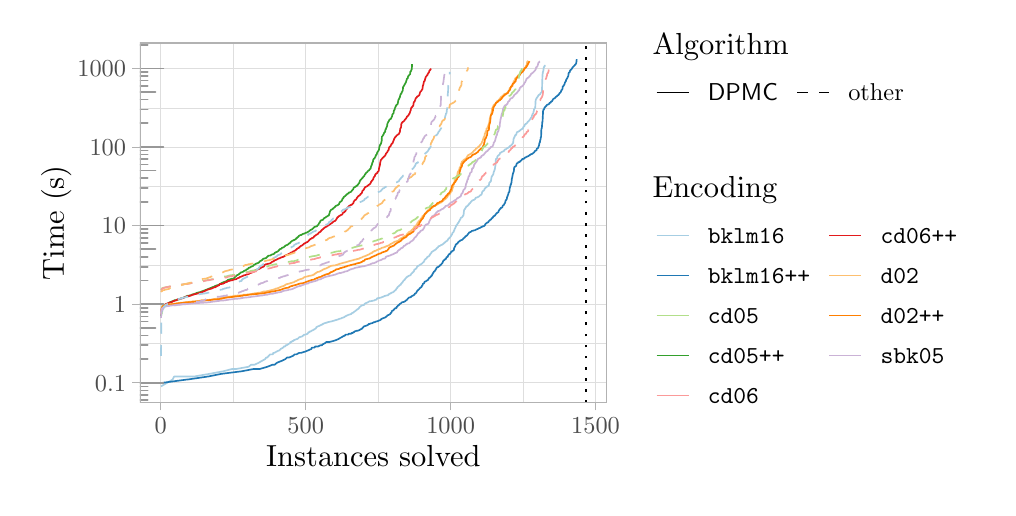
\begin{tikzpicture}[x=1pt,y=1pt]
\definecolor{fillColor}{RGB}{255,255,255}
\path[use as bounding box,fill=fillColor,fill opacity=0.00] (0,0) rectangle (346.90,166.22);
\begin{scope}
\path[clip] (  0.00,  0.00) rectangle (346.90,166.22);
\definecolor{drawColor}{RGB}{255,255,255}
\definecolor{fillColor}{RGB}{255,255,255}

\path[draw=drawColor,line width= 0.6pt,line join=round,line cap=round,fill=fillColor] (  0.00,  0.00) rectangle (346.90,166.22);
\end{scope}
\begin{scope}
\path[clip] ( 40.51, 30.69) rectangle (209.32,160.72);
\definecolor{fillColor}{RGB}{255,255,255}

\path[fill=fillColor] ( 40.51, 30.69) rectangle (209.32,160.72);
\definecolor{drawColor}{gray}{0.87}

\path[draw=drawColor,line width= 0.1pt,line join=round] ( 40.51, 52.10) --
	(209.32, 52.10);

\path[draw=drawColor,line width= 0.1pt,line join=round] ( 40.51, 80.50) --
	(209.32, 80.50);

\path[draw=drawColor,line width= 0.1pt,line join=round] ( 40.51,108.91) --
	(209.32,108.91);

\path[draw=drawColor,line width= 0.1pt,line join=round] ( 40.51,137.31) --
	(209.32,137.31);

\path[draw=drawColor,line width= 0.1pt,line join=round] ( 74.27, 30.69) --
	( 74.27,160.72);

\path[draw=drawColor,line width= 0.1pt,line join=round] (126.65, 30.69) --
	(126.65,160.72);

\path[draw=drawColor,line width= 0.1pt,line join=round] (179.02, 30.69) --
	(179.02,160.72);

\path[draw=drawColor,line width= 0.3pt,line join=round] ( 40.51, 37.90) --
	(209.32, 37.90);

\path[draw=drawColor,line width= 0.3pt,line join=round] ( 40.51, 66.30) --
	(209.32, 66.30);

\path[draw=drawColor,line width= 0.3pt,line join=round] ( 40.51, 94.71) --
	(209.32, 94.71);

\path[draw=drawColor,line width= 0.3pt,line join=round] ( 40.51,123.11) --
	(209.32,123.11);

\path[draw=drawColor,line width= 0.3pt,line join=round] ( 40.51,151.51) --
	(209.32,151.51);

\path[draw=drawColor,line width= 0.3pt,line join=round] ( 48.08, 30.69) --
	( 48.08,160.72);

\path[draw=drawColor,line width= 0.3pt,line join=round] (100.46, 30.69) --
	(100.46,160.72);

\path[draw=drawColor,line width= 0.3pt,line join=round] (152.83, 30.69) --
	(152.83,160.72);

\path[draw=drawColor,line width= 0.3pt,line join=round] (205.21, 30.69) --
	(205.21,160.72);
\definecolor{drawColor}{RGB}{166,206,227}

\path[draw=drawColor,line width= 0.6pt,line join=round] ( 48.18, 36.60) --
	( 52.37, 39.07) --
	( 52.90, 40.15) --
	( 60.02, 40.15) --
	( 65.68, 41.13) --
	( 70.60, 42.05) --
	( 73.95, 42.90) --
	( 75.42, 42.90) --
	( 79.82, 43.69) --
	( 80.76, 44.44) --
	( 82.02, 44.44) --
	( 83.49, 45.15) --
	( 84.64, 45.81) --
	( 85.79, 46.45) --
	( 86.21, 47.05) --
	( 86.63, 47.05) --
	( 87.05, 47.62) --
	( 87.15, 47.62) --
	( 87.57, 48.17) --
	( 88.62, 48.17) --
	( 88.72, 48.70) --
	( 89.14, 48.70) --
	( 89.98, 49.20) --
	( 91.03, 49.68) --
	( 91.45, 50.15) --
	( 92.29, 50.60) --
	( 92.60, 51.03) --
	( 93.02, 51.03) --
	( 93.23, 51.45) --
	( 93.54, 51.45) --
	( 94.17, 51.85) --
	( 94.80, 52.24) --
	( 94.90, 52.62) --
	( 95.32, 52.62) --
	( 95.64, 52.99) --
	( 95.95, 52.99) --
	( 96.27, 53.35) --
	( 96.37, 53.35) --
	( 97.21, 53.70) --
	( 97.42, 53.70) --
	( 97.84, 54.04) --
	( 98.15, 54.36) --
	( 99.30, 54.69) --
	( 99.51, 55.00) --
	( 99.62, 55.00) --
	( 99.93, 55.30) --
	(100.35, 55.30) --
	(101.08, 55.60) --
	(101.19, 55.60) --
	(101.29, 55.89) --
	(101.50, 56.17) --
	(101.82, 56.17) --
	(101.92, 56.45) --
	(102.34, 56.45) --
	(102.55, 56.72) --
	(102.66, 56.72) --
	(103.18, 56.99) --
	(103.28, 56.99) --
	(103.60, 57.25) --
	(104.12, 57.50) --
	(104.23, 57.75) --
	(104.33, 57.99) --
	(104.75, 58.23) --
	(105.38, 58.47) --
	(105.80, 58.70) --
	(106.43, 58.93) --
	(106.53, 59.15) --
	(106.85, 59.15) --
	(106.95, 59.37) --
	(107.16, 59.37) --
	(107.79, 59.58) --
	(108.10, 59.58) --
	(108.21, 59.79) --
	(108.42, 59.79) --
	(109.36, 60.00) --
	(109.47, 60.00) --
	(110.20, 60.20) --
	(110.83, 60.40) --
	(111.46, 60.60) --
	(111.56, 60.60) --
	(112.19, 60.80) --
	(112.61, 60.99) --
	(113.34, 61.18) --
	(113.55, 61.36) --
	(113.76, 61.36) --
	(114.18, 61.54) --
	(114.28, 61.54) --
	(114.49, 61.72) --
	(114.60, 61.72) --
	(114.70, 61.90) --
	(115.12, 62.08) --
	(115.44, 62.25) --
	(115.86, 62.42) --
	(116.38, 62.59) --
	(116.90, 62.75) --
	(117.01, 62.92) --
	(117.22, 63.08) --
	(117.64, 63.24) --
	(117.74, 63.39) --
	(117.85, 63.39) --
	(117.95, 63.55) --
	(118.16, 63.70) --
	(118.26, 63.70) --
	(118.37, 63.85) --
	(118.47, 63.85) --
	(118.58, 64.00) --
	(118.79, 64.15) --
	(119.00, 64.30) --
	(119.10, 64.44) --
	(119.42, 64.58) --
	(119.63, 64.72) --
	(119.84, 65.14) --
	(119.94, 65.27) --
	(120.36, 65.54) --
	(120.46, 65.67) --
	(120.57, 65.80) --
	(121.09, 65.93) --
	(121.62, 66.05) --
	(121.72, 66.42) --
	(122.04, 66.55) --
	(122.14, 66.67) --
	(122.46, 66.78) --
	(122.77, 66.90) --
	(122.98, 67.02) --
	(123.08, 67.14) --
	(123.19, 67.14) --
	(123.40, 67.36) --
	(123.71, 67.36) --
	(124.55, 67.48) --
	(124.76, 67.59) --
	(125.07, 67.59) --
	(125.28, 67.70) --
	(125.49, 67.81) --
	(125.81, 67.92) --
	(125.91, 67.92) --
	(126.12, 68.02) --
	(126.23, 68.34) --
	(126.33, 68.45) --
	(126.44, 68.45) --
	(126.96, 68.55) --
	(127.06, 68.55) --
	(127.38, 68.65) --
	(127.48, 68.65) --
	(127.90, 68.75) --
	(128.01, 68.85) --
	(128.32, 68.95) --
	(128.64, 69.05) --
	(128.74, 69.15) --
	(128.95, 69.25) --
	(129.37, 69.35) --
	(129.47, 69.44) --
	(129.79, 69.44) --
	(130.00, 69.54) --
	(130.31, 69.54) --
	(130.42, 69.82) --
	(130.63, 70.00) --
	(130.94, 70.09) --
	(131.04, 70.18) --
	(131.15, 70.18) --
	(131.25, 70.27) --
	(131.36, 70.36) --
	(131.46, 70.45) --
	(131.78, 70.54) --
	(131.88, 70.54) --
	(132.09, 70.71) --
	(132.20, 70.71) --
	(132.30, 70.80) --
	(132.41, 70.97) --
	(132.62, 71.14) --
	(132.72, 71.22) --
	(132.83, 71.38) --
	(133.04, 71.47) --
	(133.14, 71.55) --
	(133.24, 71.94) --
	(133.45, 72.10) --
	(133.56, 72.18) --
	(133.66, 72.48) --
	(133.77, 72.55) --
	(133.98, 72.70) --
	(134.08, 72.77) --
	(134.19, 72.92) --
	(134.29, 72.99) --
	(134.40, 73.13) --
	(134.50, 73.20) --
	(134.61, 73.27) --
	(134.82, 73.34) --
	(134.92, 73.69) --
	(135.03, 73.76) --
	(135.13, 73.96) --
	(135.34, 74.02) --
	(135.44, 74.28) --
	(135.55, 74.35) --
	(135.65, 74.60) --
	(135.76, 74.73) --
	(135.86, 74.85) --
	(135.97, 74.91) --
	(136.18, 75.10) --
	(136.28, 75.16) --
	(136.39, 75.45) --
	(136.49, 75.51) --
	(136.60, 75.69) --
	(136.70, 75.74) --
	(136.81, 75.91) --
	(136.91, 76.03) --
	(137.12, 76.14) --
	(137.23, 76.19) --
	(137.33, 76.36) --
	(137.54, 76.41) --
	(137.64, 76.52) --
	(137.75, 76.58) --
	(137.96, 76.63) --
	(138.06, 76.68) --
	(138.27, 76.74) --
	(138.38, 76.84) --
	(138.69, 77.41) --
	(138.80, 77.46) --
	(138.90, 77.51) --
	(139.01, 77.65) --
	(139.11, 77.75) --
	(139.22, 77.90) --
	(139.32, 77.94) --
	(139.53, 78.09) --
	(139.63, 78.42) --
	(139.74, 78.78) --
	(139.84, 78.82) --
	(139.95, 78.87) --
	(140.05, 78.96) --
	(140.16, 79.05) --
	(140.26, 79.09) --
	(140.37, 79.18) --
	(140.47, 79.22) --
	(140.58, 79.56) --
	(140.68, 79.77) --
	(140.79, 79.94) --
	(140.89, 79.98) --
	(141.00, 80.10) --
	(141.10, 80.18) --
	(141.21, 80.18) --
	(141.31, 80.22) --
	(141.42, 80.30) --
	(141.52, 80.34) --
	(141.63, 80.38) --
	(141.73, 80.49) --
	(141.83, 80.61) --
	(141.94, 80.69) --
	(142.15, 80.73) --
	(142.25, 80.84) --
	(142.36, 80.88) --
	(142.46, 80.95) --
	(142.67, 81.21) --
	(142.78, 81.32) --
	(142.88, 81.40) --
	(142.99, 81.47) --
	(143.09, 81.47) --
	(143.20, 81.75) --
	(143.30, 81.93) --
	(143.41, 82.20) --
	(143.51, 82.44) --
	(143.62, 82.47) --
	(143.72, 82.54) --
	(143.83, 82.67) --
	(143.93, 82.70) --
	(144.03, 82.77) --
	(144.14, 82.80) --
	(144.24, 83.09) --
	(144.35, 83.28) --
	(144.45, 83.31) --
	(144.56, 83.49) --
	(144.87, 83.52) --
	(144.98, 83.62) --
	(145.08, 83.80) --
	(145.19, 83.92) --
	(145.29, 84.00) --
	(145.40, 84.35) --
	(145.50, 84.44) --
	(145.61, 84.55) --
	(145.71, 84.63) --
	(145.82, 84.77) --
	(145.92, 85.15) --
	(146.13, 85.18) --
	(146.23, 85.29) --
	(146.34, 85.39) --
	(146.44, 85.42) --
	(146.55, 85.55) --
	(146.65, 85.60) --
	(146.76, 85.68) --
	(146.86, 85.70) --
	(146.97, 85.73) --
	(147.07, 85.80) --
	(147.18, 85.91) --
	(147.28, 85.93) --
	(147.39, 86.08) --
	(147.49, 86.13) --
	(147.60, 86.15) --
	(147.70, 86.47) --
	(147.81, 86.50) --
	(147.91, 86.59) --
	(148.02, 86.69) --
	(148.12, 86.71) --
	(148.22, 86.80) --
	(148.33, 87.04) --
	(148.43, 87.24) --
	(148.54, 87.26) --
	(148.64, 87.29) --
	(148.75, 87.31) --
	(148.85, 87.33) --
	(148.96, 87.40) --
	(149.06, 87.40) --
	(149.17, 87.53) --
	(149.27, 87.57) --
	(149.38, 87.68) --
	(149.48, 87.71) --
	(149.59, 87.73) --
	(149.69, 87.79) --
	(149.80, 87.81) --
	(149.90, 87.94) --
	(150.01, 87.99) --
	(150.11, 88.05) --
	(150.22, 88.09) --
	(150.32, 88.22) --
	(150.42, 88.40) --
	(150.63, 88.42) --
	(150.74, 88.61) --
	(150.84, 88.71) --
	(150.95, 88.77) --
	(151.05, 88.93) --
	(151.16, 88.97) --
	(151.26, 88.99) --
	(151.37, 89.08) --
	(151.47, 89.12) --
	(151.58, 89.24) --
	(151.68, 89.32) --
	(151.79, 89.54) --
	(151.89, 89.60) --
	(152.00, 89.93) --
	(152.10, 89.97) --
	(152.21, 90.00) --
	(152.42, 90.34) --
	(152.62, 90.38) --
	(152.73, 90.60) --
	(152.83, 90.70) --
	(152.94, 90.87) --
	(153.04, 91.22) --
	(153.15, 91.24) --
	(153.25, 91.38) --
	(153.36, 91.50) --
	(153.46, 92.04) --
	(153.57, 92.11) --
	(153.67, 92.21) --
	(153.78, 92.29) --
	(153.88, 92.30) --
	(153.99, 92.74) --
	(154.09, 92.87) --
	(154.20, 93.11) --
	(154.30, 93.56) --
	(154.41, 93.58) --
	(154.51, 93.90) --
	(154.61, 94.16) --
	(154.72, 94.19) --
	(154.82, 94.72) --
	(155.03, 94.83) --
	(155.14, 95.02) --
	(155.24, 95.08) --
	(155.35, 95.51) --
	(155.45, 95.53) --
	(155.56, 95.67) --
	(155.66, 95.77) --
	(155.77, 95.93) --
	(155.87, 96.21) --
	(155.98, 96.34) --
	(156.08, 96.63) --
	(156.19, 96.71) --
	(156.29, 96.95) --
	(156.40, 97.06) --
	(156.50, 97.48) --
	(156.61, 97.55) --
	(156.71, 97.59) --
	(156.81, 97.62) --
	(156.92, 97.67) --
	(157.02, 97.85) --
	(157.13, 97.88) --
	(157.23, 98.03) --
	(157.34, 98.32) --
	(157.44, 98.34) --
	(157.55, 98.94) --
	(157.65, 99.96) --
	(157.76,100.50) --
	(157.86,100.51) --
	(157.97,100.69) --
	(158.07,100.76) --
	(158.18,101.05) --
	(158.28,101.21) --
	(158.39,101.35) --
	(158.49,101.61) --
	(158.60,101.64) --
	(158.70,101.67) --
	(158.81,101.71) --
	(158.91,101.81) --
	(159.01,101.93) --
	(159.12,101.95) --
	(159.22,102.19) --
	(159.33,102.24) --
	(159.43,102.33) --
	(159.54,102.67) --
	(159.64,102.69) --
	(159.75,102.70) --
	(159.85,102.82) --
	(159.96,102.99) --
	(160.06,103.06) --
	(160.17,103.27) --
	(160.27,103.38) --
	(160.38,103.52) --
	(160.48,103.55) --
	(160.59,103.70) --
	(160.69,103.80) --
	(160.80,103.81) --
	(160.90,103.90) --
	(161.01,103.93) --
	(161.11,103.95) --
	(161.21,104.00) --
	(161.32,104.02) --
	(161.42,104.09) --
	(161.53,104.23) --
	(161.63,104.24) --
	(161.74,104.44) --
	(161.84,104.63) --
	(161.95,104.80) --
	(162.05,104.81) --
	(162.16,104.83) --
	(162.26,104.85) --
	(162.47,104.90) --
	(162.58,104.92) --
	(162.68,105.04) --
	(162.79,105.05) --
	(162.89,105.11) --
	(163.00,105.18) --
	(163.10,105.25) --
	(163.20,105.30) --
	(163.31,105.45) --
	(163.41,105.57) --
	(163.52,105.65) --
	(163.62,105.72) --
	(163.73,105.77) --
	(163.83,105.79) --
	(163.94,105.90) --
	(164.04,106.03) --
	(164.15,106.46) --
	(164.25,106.85) --
	(164.36,107.01) --
	(164.46,107.11) --
	(164.57,107.21) --
	(164.67,107.30) --
	(164.78,107.35) --
	(164.88,107.43) --
	(164.99,107.55) --
	(165.09,107.95) --
	(165.20,107.99) --
	(165.30,108.29) --
	(165.40,108.32) --
	(165.51,108.34) --
	(165.61,108.56) --
	(165.72,108.57) --
	(165.82,108.59) --
	(165.93,108.77) --
	(166.03,108.90) --
	(166.14,108.92) --
	(166.24,108.93) --
	(166.35,108.97) --
	(166.45,109.00) --
	(166.56,109.07) --
	(166.66,109.25) --
	(166.77,110.06) --
	(166.87,110.25) --
	(166.98,110.26) --
	(167.08,110.48) --
	(167.19,110.51) --
	(167.29,110.53) --
	(167.40,110.88) --
	(167.50,111.51) --
	(167.60,112.18) --
	(167.71,112.46) --
	(167.81,112.57) --
	(167.92,112.78) --
	(168.02,112.93) --
	(168.13,113.05) --
	(168.23,113.19) --
	(168.34,113.75) --
	(168.44,114.16) --
	(168.55,114.34) --
	(168.65,114.71) --
	(168.76,114.86) --
	(168.86,115.40) --
	(168.97,116.25) --
	(169.07,116.58) --
	(169.18,118.67) --
	(169.28,118.80) --
	(169.39,118.83) --
	(169.49,118.87) --
	(169.59,118.95) --
	(169.70,119.57) --
	(169.80,119.71) --
	(169.91,119.90) --
	(170.01,120.00) --
	(170.12,120.07) --
	(170.22,120.17) --
	(170.33,120.20) --
	(170.43,120.31) --
	(170.54,120.44) --
	(170.64,120.79) --
	(170.75,120.97) --
	(170.85,121.04) --
	(170.96,121.06) --
	(171.06,121.17) --
	(171.17,121.17) --
	(171.27,121.28) --
	(171.38,121.31) --
	(171.48,121.35) --
	(171.59,121.46) --
	(171.69,121.48) --
	(171.79,121.51) --
	(171.90,121.57) --
	(172.00,121.58) --
	(172.11,121.70) --
	(172.21,121.85) --
	(172.32,122.11) --
	(172.42,122.19) --
	(172.53,122.22) --
	(172.63,122.23) --
	(172.74,122.29) --
	(172.84,122.30) --
	(172.95,122.44) --
	(173.05,122.45) --
	(173.16,122.61) --
	(173.26,122.72) --
	(173.37,122.72) --
	(173.47,122.75) --
	(173.58,122.79) --
	(173.68,122.90) --
	(173.79,122.95) --
	(173.89,122.99) --
	(173.99,123.09) --
	(174.10,123.23) --
	(174.20,123.29) --
	(174.31,123.46) --
	(174.41,123.50) --
	(174.52,123.51) --
	(174.62,123.69) --
	(174.73,123.75) --
	(174.83,123.77) --
	(174.94,123.94) --
	(175.04,124.06) --
	(175.15,124.25) --
	(175.25,124.37) --
	(175.36,124.46) --
	(175.46,124.88) --
	(175.57,125.99) --
	(175.67,126.22) --
	(175.78,126.43) --
	(175.88,126.74) --
	(175.99,126.85) --
	(176.09,127.12) --
	(176.19,127.43) --
	(176.30,127.44) --
	(176.40,127.45) --
	(176.51,127.48) --
	(176.61,127.88) --
	(176.72,128.25) --
	(176.82,128.46) --
	(176.93,128.52) --
	(177.03,128.59) --
	(177.24,128.59) --
	(177.35,128.67) --
	(177.45,128.79) --
	(177.56,128.80) --
	(177.66,128.84) --
	(177.77,128.99) --
	(177.87,129.02) --
	(177.98,129.15) --
	(178.08,129.29) --
	(178.18,129.36) --
	(178.29,129.38) --
	(178.39,129.44) --
	(178.50,129.53) --
	(178.60,129.59) --
	(178.71,129.64) --
	(178.81,129.68) --
	(178.92,129.85) --
	(179.02,130.04) --
	(179.13,130.33) --
	(179.23,130.46) --
	(179.34,130.59) --
	(179.44,130.65) --
	(179.55,130.65) --
	(179.65,131.11) --
	(179.76,131.29) --
	(179.86,131.35) --
	(179.97,131.45) --
	(180.07,131.46) --
	(180.18,131.56) --
	(180.28,131.56) --
	(180.38,131.77) --
	(180.49,131.82) --
	(180.59,132.04) --
	(180.70,132.17) --
	(180.80,132.28) --
	(180.91,132.35) --
	(181.01,132.44) --
	(181.12,132.55) --
	(181.22,132.66) --
	(181.33,132.83) --
	(181.43,132.95) --
	(181.54,133.21) --
	(181.64,133.22) --
	(181.75,133.47) --
	(181.85,133.61) --
	(181.96,133.75) --
	(182.06,133.89) --
	(182.17,134.05) --
	(182.27,134.59) --
	(182.38,134.83) --
	(182.48,135.05) --
	(182.58,135.12) --
	(182.69,135.22) --
	(182.79,135.91) --
	(182.90,136.10) --
	(183.00,136.84) --
	(183.11,136.88) --
	(183.21,137.06) --
	(183.32,137.16) --
	(183.42,137.47) --
	(183.53,139.73) --
	(183.63,140.25) --
	(183.74,140.39) --
	(183.84,140.53) --
	(183.95,140.91) --
	(184.05,140.96) --
	(184.16,140.96) --
	(184.26,141.31) --
	(184.37,141.37) --
	(184.47,141.68) --
	(184.57,141.75) --
	(184.68,141.82) --
	(184.78,142.02) --
	(184.89,142.04) --
	(184.99,142.08) --
	(185.10,142.10) --
	(185.20,142.18) --
	(185.31,142.56) --
	(185.41,142.60) --
	(185.52,142.75) --
	(185.62,142.83) --
	(185.73,143.02) --
	(185.83,143.07) --
	(185.94,147.02) --
	(186.04,149.16) --
	(186.15,150.01) --
	(186.25,150.41) --
	(186.36,150.79) --
	(186.46,151.75) --
	(186.57,151.92) --
	(186.67,152.18) --
	(186.77,152.34) --
	(186.88,152.44) --
	(186.98,152.54) --
	(187.09,152.60);
\definecolor{drawColor}{RGB}{31,120,180}

\path[draw=drawColor,line width= 0.6pt,line join=round] ( 48.81, 37.90) --
	( 57.51, 39.07) --
	( 57.72, 39.07) --
	( 65.05, 40.15) --
	( 65.15, 40.15) --
	( 69.97, 41.13) --
	( 77.31, 42.05) --
	( 81.71, 42.90) --
	( 83.91, 42.90) --
	( 86.63, 43.69) --
	( 88.51, 44.44) --
	( 89.25, 44.44) --
	( 90.09, 45.15) --
	( 91.76, 45.81) --
	( 93.12, 46.45) --
	( 93.75, 47.05) --
	( 94.49, 47.05) --
	( 95.85, 47.62) --
	( 96.48, 48.17) --
	( 97.10, 48.17) --
	( 98.15, 48.70) --
	( 98.78, 48.70) --
	(100.35, 49.20) --
	(101.50, 49.68) --
	(102.55, 50.15) --
	(102.66, 50.60) --
	(103.60, 50.60) --
	(103.91, 51.03) --
	(104.96, 51.03) --
	(105.80, 51.45) --
	(106.32, 51.45) --
	(106.64, 51.85) --
	(106.74, 51.85) --
	(107.48, 52.24) --
	(107.89, 52.62) --
	(108.94, 52.62) --
	(110.41, 52.99) --
	(111.46, 53.35) --
	(112.29, 53.70) --
	(112.82, 54.04) --
	(113.45, 54.36) --
	(113.97, 54.69) --
	(114.70, 55.00) --
	(114.81, 55.30) --
	(115.86, 55.30) --
	(115.96, 55.60) --
	(116.90, 55.60) --
	(117.01, 55.89) --
	(117.43, 55.89) --
	(117.64, 56.17) --
	(117.95, 56.17) --
	(118.06, 56.45) --
	(118.16, 56.45) --
	(119.00, 56.72) --
	(119.31, 56.72) --
	(119.94, 56.99) --
	(120.05, 56.99) --
	(120.26, 57.25) --
	(120.36, 57.25) --
	(120.88, 57.50) --
	(120.99, 57.75) --
	(121.30, 57.99) --
	(121.41, 58.23) --
	(122.14, 58.47) --
	(122.77, 58.70) --
	(123.08, 58.93) --
	(123.19, 59.15) --
	(123.61, 59.15) --
	(123.92, 59.37) --
	(124.24, 59.37) --
	(124.76, 59.58) --
	(125.07, 59.79) --
	(125.28, 59.79) --
	(125.81, 60.00) --
	(126.54, 60.20) --
	(126.96, 60.40) --
	(127.48, 60.60) --
	(127.69, 60.80) --
	(127.80, 60.99) --
	(128.32, 61.18) --
	(128.74, 61.36) --
	(128.95, 61.36) --
	(129.16, 61.54) --
	(129.47, 61.72) --
	(129.68, 61.90) --
	(129.89, 62.08) --
	(130.00, 62.25) --
	(130.42, 62.42) --
	(130.73, 62.59) --
	(131.04, 62.75) --
	(131.15, 63.08) --
	(131.46, 63.24) --
	(131.57, 63.85) --
	(131.78, 63.85) --
	(131.88, 64.00) --
	(132.09, 64.00) --
	(132.20, 64.15) --
	(132.30, 64.30) --
	(132.41, 64.44) --
	(132.62, 64.72) --
	(132.93, 64.86) --
	(133.14, 64.86) --
	(133.24, 64.86) --
	(133.35, 65.41) --
	(133.56, 65.41) --
	(133.66, 65.54) --
	(133.77, 65.80) --
	(133.98, 65.93) --
	(134.08, 65.93) --
	(134.19, 66.05) --
	(134.40, 66.30) --
	(134.50, 66.42) --
	(134.82, 66.55) --
	(135.03, 66.78) --
	(135.13, 66.90) --
	(135.44, 67.02) --
	(135.97, 67.14) --
	(136.18, 67.25) --
	(136.39, 67.36) --
	(136.60, 67.59) --
	(136.81, 67.70) --
	(136.91, 67.81) --
	(137.02, 67.81) --
	(137.23, 68.13) --
	(137.33, 68.24) --
	(137.44, 68.34) --
	(137.54, 68.45) --
	(137.64, 68.55) --
	(137.75, 68.65) --
	(137.96, 68.75) --
	(138.48, 68.85) --
	(138.59, 69.05) --
	(138.69, 69.15) --
	(138.90, 69.25) --
	(139.11, 69.35) --
	(139.22, 69.44) --
	(139.43, 69.54) --
	(139.63, 69.63) --
	(139.74, 69.73) --
	(139.84, 69.91) --
	(139.95, 70.18) --
	(140.16, 70.18) --
	(140.37, 70.36) --
	(140.47, 70.54) --
	(140.58, 70.80) --
	(140.68, 70.97) --
	(140.79, 71.14) --
	(140.89, 71.22) --
	(141.00, 71.30) --
	(141.10, 71.47) --
	(141.21, 71.55) --
	(141.31, 71.63) --
	(141.42, 71.71) --
	(141.52, 71.79) --
	(141.63, 72.02) --
	(141.73, 72.10) --
	(141.83, 72.18) --
	(142.15, 72.40) --
	(142.25, 72.48) --
	(142.36, 72.63) --
	(142.46, 72.92) --
	(142.57, 72.99) --
	(142.67, 73.06) --
	(142.78, 73.62) --
	(142.99, 73.69) --
	(143.09, 73.76) --
	(143.20, 73.89) --
	(143.30, 74.02) --
	(143.41, 74.35) --
	(143.51, 74.41) --
	(143.62, 74.48) --
	(143.83, 74.54) --
	(143.93, 74.60) --
	(144.03, 74.66) --
	(144.14, 74.79) --
	(144.24, 74.85) --
	(144.35, 74.91) --
	(144.45, 74.91) --
	(144.66, 75.10) --
	(144.77, 75.22) --
	(144.87, 75.51) --
	(144.98, 75.69) --
	(145.08, 75.74) --
	(145.19, 75.80) --
	(145.29, 75.91) --
	(145.50, 76.03) --
	(145.61, 76.25) --
	(145.71, 76.30) --
	(145.82, 76.47) --
	(145.92, 76.52) --
	(146.03, 76.58) --
	(146.23, 77.15) --
	(146.34, 77.20) --
	(146.44, 77.51) --
	(146.55, 77.60) --
	(146.65, 77.70) --
	(146.76, 78.04) --
	(146.97, 78.18) --
	(147.18, 78.32) --
	(147.28, 78.55) --
	(147.39, 78.60) --
	(147.49, 79.00) --
	(147.60, 79.05) --
	(147.70, 79.26) --
	(147.81, 79.56) --
	(147.91, 79.56) --
	(148.02, 79.65) --
	(148.22, 79.69) --
	(148.33, 79.73) --
	(148.43, 79.89) --
	(148.54, 79.89) --
	(148.64, 79.98) --
	(148.75, 80.06) --
	(148.85, 80.06) --
	(148.96, 80.30) --
	(149.06, 80.42) --
	(149.17, 80.46) --
	(149.27, 80.49) --
	(149.38, 80.53) --
	(149.48, 80.80) --
	(149.69, 80.99) --
	(149.80, 81.18) --
	(149.90, 81.18) --
	(150.01, 81.54) --
	(150.11, 81.79) --
	(150.22, 82.00) --
	(150.42, 82.20) --
	(150.53, 82.24) --
	(150.63, 82.24) --
	(150.74, 82.51) --
	(150.84, 82.54) --
	(150.95, 82.57) --
	(151.05, 82.67) --
	(151.16, 82.74) --
	(151.26, 83.03) --
	(151.37, 83.31) --
	(151.58, 83.34) --
	(151.68, 83.37) --
	(151.79, 83.40) --
	(151.89, 83.80) --
	(152.00, 84.03) --
	(152.10, 84.06) --
	(152.21, 84.35) --
	(152.31, 84.38) --
	(152.42, 84.41) --
	(152.52, 84.47) --
	(152.62, 84.52) --
	(152.73, 84.55) --
	(152.83, 84.80) --
	(152.94, 85.13) --
	(153.04, 85.15) --
	(153.15, 85.18) --
	(153.25, 85.31) --
	(153.36, 85.44) --
	(153.46, 85.55) --
	(153.67, 85.60) --
	(153.78, 85.68) --
	(153.99, 85.80) --
	(154.09, 86.54) --
	(154.20, 86.71) --
	(154.30, 86.87) --
	(154.41, 87.13) --
	(154.51, 87.17) --
	(154.61, 87.68) --
	(154.72, 87.86) --
	(154.82, 87.96) --
	(154.93, 88.01) --
	(155.03, 88.07) --
	(155.14, 88.20) --
	(155.24, 88.22) --
	(155.35, 88.24) --
	(155.45, 88.59) --
	(155.56, 88.63) --
	(155.66, 88.83) --
	(155.77, 88.87) --
	(155.87, 88.95) --
	(155.98, 89.01) --
	(156.08, 89.04) --
	(156.19, 89.14) --
	(156.29, 89.33) --
	(156.40, 89.33) --
	(156.50, 89.37) --
	(156.61, 89.41) --
	(156.71, 89.43) --
	(156.81, 89.47) --
	(156.92, 89.52) --
	(157.02, 89.56) --
	(157.13, 89.65) --
	(157.23, 89.80) --
	(157.34, 89.82) --
	(157.44, 90.09) --
	(157.55, 90.11) --
	(157.65, 90.22) --
	(157.76, 90.31) --
	(157.86, 90.36) --
	(157.97, 90.52) --
	(158.07, 90.53) --
	(158.18, 90.79) --
	(158.28, 90.89) --
	(158.39, 90.91) --
	(158.49, 90.97) --
	(158.60, 91.06) --
	(158.70, 91.09) --
	(158.81, 91.17) --
	(158.91, 91.37) --
	(159.01, 91.48) --
	(159.12, 91.69) --
	(159.22, 91.78) --
	(159.33, 91.88) --
	(159.43, 92.01) --
	(159.54, 92.26) --
	(159.64, 92.27) --
	(159.75, 92.30) --
	(159.96, 92.36) --
	(160.06, 92.39) --
	(160.17, 92.42) --
	(160.27, 92.53) --
	(160.38, 92.69) --
	(160.48, 92.76) --
	(160.59, 92.79) --
	(160.69, 92.80) --
	(160.80, 92.82) --
	(160.90, 92.84) --
	(161.01, 92.89) --
	(161.11, 92.93) --
	(161.21, 92.96) --
	(161.53, 92.99) --
	(161.63, 93.00) --
	(161.74, 93.11) --
	(161.84, 93.13) --
	(161.95, 93.23) --
	(162.05, 93.27) --
	(162.16, 93.31) --
	(162.26, 93.36) --
	(162.37, 93.41) --
	(162.47, 93.42) --
	(162.58, 93.46) --
	(162.68, 93.57) --
	(162.79, 93.57) --
	(162.89, 93.60) --
	(163.00, 93.73) --
	(163.10, 93.77) --
	(163.20, 93.80) --
	(163.31, 93.81) --
	(163.41, 93.85) --
	(163.52, 93.90) --
	(163.62, 93.97) --
	(163.73, 94.06) --
	(163.83, 94.12) --
	(163.94, 94.15) --
	(164.04, 94.27) --
	(164.25, 94.27) --
	(164.36, 94.35) --
	(164.46, 94.42) --
	(164.57, 94.47) --
	(164.67, 94.47) --
	(164.78, 94.48) --
	(164.88, 94.52) --
	(164.99, 94.61) --
	(165.09, 94.64) --
	(165.20, 94.83) --
	(165.30, 94.95) --
	(165.40, 95.24) --
	(165.51, 95.41) --
	(165.61, 95.42) --
	(165.72, 95.59) --
	(165.93, 95.62) --
	(166.03, 95.80) --
	(166.14, 95.84) --
	(166.24, 95.86) --
	(166.35, 95.88) --
	(166.45, 95.95) --
	(166.56, 96.23) --
	(166.66, 96.32) --
	(166.77, 96.43) --
	(166.87, 96.46) --
	(166.98, 96.61) --
	(167.08, 96.76) --
	(167.19, 96.78) --
	(167.29, 96.82) --
	(167.40, 96.89) --
	(167.50, 96.93) --
	(167.60, 97.28) --
	(167.71, 97.33) --
	(167.81, 97.45) --
	(167.92, 97.48) --
	(168.02, 97.54) --
	(168.13, 97.63) --
	(168.23, 97.97) --
	(168.34, 98.05) --
	(168.44, 98.13) --
	(168.55, 98.15) --
	(168.65, 98.20) --
	(168.76, 98.27) --
	(168.86, 98.35) --
	(168.97, 98.58) --
	(169.07, 98.65) --
	(169.18, 98.88) --
	(169.28, 98.90) --
	(169.39, 99.16) --
	(169.49, 99.19) --
	(169.59, 99.21) --
	(169.70, 99.34) --
	(169.80, 99.38) --
	(169.91, 99.49) --
	(170.01, 99.52) --
	(170.12, 99.61) --
	(170.22,100.10) --
	(170.33,100.11) --
	(170.43,100.40) --
	(170.54,100.52) --
	(170.64,100.68) --
	(170.75,100.71) --
	(170.85,100.81) --
	(170.96,101.09) --
	(171.06,101.12) --
	(171.17,101.13) --
	(171.27,101.20) --
	(171.38,101.25) --
	(171.48,101.26) --
	(171.59,101.56) --
	(171.69,101.98) --
	(171.79,101.99) --
	(171.90,102.09) --
	(172.00,102.14) --
	(172.11,102.19) --
	(172.21,102.39) --
	(172.32,102.75) --
	(172.42,102.76) --
	(172.53,103.00) --
	(172.63,103.54) --
	(172.74,103.82) --
	(172.84,103.92) --
	(172.95,103.96) --
	(173.05,104.19) --
	(173.16,104.47) --
	(173.26,105.15) --
	(173.37,105.17) --
	(173.47,105.66) --
	(173.58,105.71) --
	(173.68,106.14) --
	(173.79,106.68) --
	(173.89,106.69) --
	(173.99,106.86) --
	(174.10,107.20) --
	(174.20,108.49) --
	(174.31,108.55) --
	(174.41,108.96) --
	(174.52,109.49) --
	(174.62,109.56) --
	(174.73,110.00) --
	(174.83,110.29) --
	(174.94,111.55) --
	(175.04,111.92) --
	(175.15,112.47) --
	(175.25,112.99) --
	(175.36,113.54) --
	(175.46,113.79) --
	(175.57,114.04) --
	(175.67,114.31) --
	(175.78,115.60) --
	(175.88,115.80) --
	(175.99,115.87) --
	(176.09,116.01) --
	(176.19,116.08) --
	(176.30,116.13) --
	(176.40,116.20) --
	(176.51,116.28) --
	(176.61,116.79) --
	(176.72,117.06) --
	(176.82,117.25) --
	(176.93,117.25) --
	(177.03,117.29) --
	(177.14,117.33) --
	(177.24,117.64) --
	(177.45,117.65) --
	(177.56,117.69) --
	(177.66,117.69) --
	(177.77,117.70) --
	(177.87,117.80) --
	(177.98,118.03) --
	(178.08,118.11) --
	(178.29,118.19) --
	(178.39,118.35) --
	(178.50,118.35) --
	(178.60,118.59) --
	(178.71,118.74) --
	(178.81,118.75) --
	(178.92,118.76) --
	(179.02,118.79) --
	(179.13,118.79) --
	(179.23,118.86) --
	(179.34,118.87) --
	(179.44,119.00) --
	(179.55,119.09) --
	(179.65,119.22) --
	(179.76,119.28) --
	(179.86,119.31) --
	(179.97,119.38) --
	(180.07,119.40) --
	(180.18,119.54) --
	(180.28,119.55) --
	(180.38,119.56) --
	(180.49,119.62) --
	(180.59,119.69) --
	(180.70,119.70) --
	(180.80,119.78) --
	(180.91,119.80) --
	(181.01,119.90) --
	(181.12,119.94) --
	(181.22,120.04) --
	(181.33,120.09) --
	(181.43,120.13) --
	(181.54,120.34) --
	(181.64,120.34) --
	(181.75,120.37) --
	(181.85,120.50) --
	(181.96,120.53) --
	(182.06,120.55) --
	(182.17,120.59) --
	(182.27,120.62) --
	(182.38,120.64) --
	(182.48,120.72) --
	(182.58,120.80) --
	(182.69,120.93) --
	(182.79,121.00) --
	(182.90,121.09) --
	(183.00,121.11) --
	(183.11,121.28) --
	(183.21,121.54) --
	(183.32,121.66) --
	(183.42,121.74) --
	(183.53,121.76) --
	(183.63,121.81) --
	(183.74,121.86) --
	(183.84,121.86) --
	(183.95,122.42) --
	(184.05,122.52) --
	(184.16,122.59) --
	(184.26,122.63) --
	(184.37,122.70) --
	(184.47,122.81) --
	(184.57,123.25) --
	(184.68,123.46) --
	(184.78,123.72) --
	(184.89,124.43) --
	(184.99,124.62) --
	(185.10,124.77) --
	(185.20,125.67) --
	(185.31,125.69) --
	(185.41,126.63) --
	(185.52,126.72) --
	(185.62,129.71) --
	(185.73,129.75) --
	(185.83,130.38) --
	(185.94,132.02) --
	(186.04,132.22) --
	(186.15,134.24) --
	(186.25,136.31) --
	(186.36,136.47) --
	(186.46,136.61) --
	(186.57,136.70) --
	(186.67,137.12) --
	(186.77,137.26) --
	(186.88,137.32) --
	(186.98,137.55) --
	(187.09,137.67) --
	(187.19,137.67) --
	(187.30,137.91) --
	(187.40,137.98) --
	(187.51,138.03) --
	(187.61,138.26) --
	(187.72,138.37) --
	(187.82,138.40) --
	(187.93,138.42) --
	(188.03,138.49) --
	(188.14,138.50) --
	(188.24,138.54) --
	(188.35,138.64) --
	(188.45,138.67) --
	(188.56,138.98) --
	(188.66,139.05) --
	(188.77,139.09) --
	(188.87,139.10) --
	(188.97,139.16) --
	(189.08,139.43) --
	(189.18,139.53) --
	(189.29,139.55) --
	(189.39,139.58) --
	(189.50,139.59) --
	(189.60,139.95) --
	(189.71,140.00) --
	(189.81,140.29) --
	(189.92,140.46) --
	(190.02,140.54) --
	(190.13,140.58) --
	(190.23,140.61) --
	(190.34,140.63) --
	(190.44,140.68) --
	(190.55,140.84) --
	(190.65,140.92) --
	(190.76,141.11) --
	(190.86,141.16) --
	(190.97,141.31) --
	(191.07,141.36) --
	(191.17,141.40) --
	(191.28,141.43) --
	(191.38,141.71) --
	(191.49,141.73) --
	(191.59,141.78) --
	(191.70,141.82) --
	(191.80,141.96) --
	(191.91,142.00) --
	(192.01,142.23) --
	(192.12,142.38) --
	(192.22,142.60) --
	(192.33,142.69) --
	(192.43,142.70) --
	(192.54,142.76) --
	(192.64,143.00) --
	(192.75,143.27) --
	(192.85,143.63) --
	(192.96,143.71) --
	(193.06,143.76) --
	(193.16,143.83) --
	(193.27,144.32) --
	(193.37,145.01) --
	(193.48,145.04) --
	(193.58,145.05) --
	(193.69,145.31) --
	(193.79,145.50) --
	(193.90,145.59) --
	(194.00,145.82) --
	(194.11,146.29) --
	(194.21,146.55) --
	(194.32,146.62) --
	(194.42,146.77) --
	(194.53,147.11) --
	(194.63,147.58) --
	(194.74,147.59) --
	(194.84,147.81) --
	(194.95,147.84) --
	(195.05,148.20) --
	(195.16,148.44) --
	(195.26,148.65) --
	(195.36,148.70) --
	(195.47,149.82) --
	(195.57,149.95) --
	(195.68,150.06) --
	(195.78,150.09) --
	(195.89,150.17) --
	(195.99,150.78) --
	(196.10,150.87) --
	(196.20,150.88) --
	(196.31,151.05) --
	(196.41,151.07) --
	(196.52,151.19) --
	(196.62,151.37) --
	(196.73,151.52) --
	(196.83,151.79) --
	(196.94,151.89) --
	(197.04,151.99) --
	(197.15,152.09) --
	(197.25,152.18) --
	(197.36,152.34) --
	(197.46,152.40) --
	(197.56,152.54) --
	(197.67,152.63) --
	(197.77,152.77) --
	(197.88,152.88) --
	(197.98,153.07) --
	(198.09,153.10) --
	(198.19,153.26) --
	(198.30,154.01) --
	(198.40,154.81);
\definecolor{drawColor}{RGB}{51,160,44}

\path[draw=drawColor,line width= 0.6pt,line join=round] ( 48.18, 61.90) --
	( 48.29, 62.42) --
	( 48.39, 63.39) --
	( 48.60, 64.30) --
	( 48.71, 65.67) --
	( 48.81, 65.80) --
	( 48.92, 65.93) --
	( 49.02, 65.93) --
	( 49.23, 66.05) --
	( 49.34, 66.05) --
	( 49.75, 66.18) --
	( 50.17, 66.30) --
	( 50.38, 66.42) --
	( 50.70, 66.55) --
	( 51.01, 66.78) --
	( 51.12, 66.90) --
	( 51.43, 67.02) --
	( 51.75, 67.14) --
	( 52.06, 67.25) --
	( 52.16, 67.36) --
	( 52.37, 67.36) --
	( 52.79, 67.48) --
	( 52.90, 67.70) --
	( 53.32, 67.70) --
	( 53.63, 67.81) --
	( 54.15, 67.92) --
	( 54.26, 68.02) --
	( 54.68, 68.02) --
	( 54.78, 68.13) --
	( 54.89, 68.13) --
	( 54.99, 68.24) --
	( 55.10, 68.24) --
	( 55.31, 68.34) --
	( 55.41, 68.34) --
	( 55.62, 68.45) --
	( 55.83, 68.45) --
	( 55.94, 68.55) --
	( 56.35, 68.65) --
	( 56.46, 68.75) --
	( 56.77, 68.85) --
	( 56.88, 68.85) --
	( 56.98, 68.95) --
	( 57.19, 69.05) --
	( 57.30, 69.15) --
	( 57.72, 69.25) --
	( 57.82, 69.35) --
	( 58.34, 69.35) --
	( 58.45, 69.44) --
	( 58.66, 69.44) --
	( 58.76, 69.54) --
	( 58.97, 69.54) --
	( 59.18, 69.63) --
	( 59.29, 69.73) --
	( 59.39, 69.73) --
	( 59.50, 69.82) --
	( 59.60, 69.82) --
	( 59.71, 69.91) --
	( 60.13, 69.91) --
	( 60.23, 70.00) --
	( 60.44, 70.09) --
	( 60.65, 70.09) --
	( 60.75, 70.18) --
	( 60.86, 70.27) --
	( 61.07, 70.36) --
	( 61.28, 70.45) --
	( 61.49, 70.45) --
	( 61.59, 70.54) --
	( 61.80, 70.54) --
	( 62.01, 70.63) --
	( 62.64, 70.71) --
	( 62.74, 70.88) --
	( 63.06, 70.97) --
	( 63.16, 70.97) --
	( 63.27, 71.05) --
	( 63.48, 71.14) --
	( 63.79, 71.22) --
	( 64.00, 71.30) --
	( 64.11, 71.38) --
	( 64.42, 71.47) --
	( 64.63, 71.55) --
	( 64.84, 71.63) --
	( 65.05, 71.71) --
	( 65.26, 71.79) --
	( 65.36, 71.87) --
	( 65.57, 71.94) --
	( 65.68, 72.02) --
	( 65.78, 72.02) --
	( 65.99, 72.10) --
	( 66.10, 72.18) --
	( 66.31, 72.18) --
	( 66.41, 72.25) --
	( 66.52, 72.33) --
	( 66.62, 72.40) --
	( 66.83, 72.48) --
	( 67.14, 72.55) --
	( 67.25, 72.55) --
	( 67.35, 72.63) --
	( 67.46, 72.70) --
	( 67.56, 72.77) --
	( 67.67, 72.85) --
	( 67.77, 72.92) --
	( 67.88, 72.92) --
	( 67.98, 72.99) --
	( 68.30, 73.06) --
	( 68.40, 73.13) --
	( 68.51, 73.13) --
	( 68.61, 73.13) --
	( 68.72, 73.20) --
	( 68.93, 73.27) --
	( 69.03, 73.34) --
	( 69.24, 73.41) --
	( 69.34, 73.55) --
	( 69.45, 73.62) --
	( 69.66, 73.69) --
	( 69.76, 73.69) --
	( 69.87, 73.76) --
	( 69.97, 73.89) --
	( 70.08, 73.96) --
	( 70.29, 74.02) --
	( 70.39, 74.09) --
	( 70.60, 74.09) --
	( 70.71, 74.28) --
	( 70.92, 74.28) --
	( 71.02, 74.35) --
	( 71.23, 74.41) --
	( 71.44, 74.48) --
	( 71.54, 74.54) --
	( 71.65, 74.54) --
	( 71.75, 74.60) --
	( 71.86, 74.66) --
	( 71.96, 74.73) --
	( 72.07, 74.79) --
	( 72.17, 74.85) --
	( 72.28, 74.97) --
	( 72.38, 75.10) --
	( 72.59, 75.16) --
	( 72.91, 75.22) --
	( 73.12, 75.28) --
	( 73.43, 75.39) --
	( 73.53, 75.45) --
	( 73.64, 75.45) --
	( 73.85, 75.51) --
	( 73.95, 75.51) --
	( 74.37, 75.57) --
	( 74.48, 75.63) --
	( 74.58, 75.69) --
	( 74.69, 75.80) --
	( 74.90, 76.08) --
	( 75.00, 76.30) --
	( 75.21, 76.41) --
	( 75.32, 76.47) --
	( 75.42, 76.68) --
	( 75.52, 76.68) --
	( 75.73, 76.79) --
	( 75.84, 76.84) --
	( 75.94, 76.89) --
	( 76.15, 76.95) --
	( 76.36, 77.15) --
	( 76.47, 77.30) --
	( 76.57, 77.35) --
	( 76.68, 77.46) --
	( 76.78, 77.51) --
	( 76.89, 77.65) --
	( 76.99, 77.75) --
	( 77.31, 77.80) --
	( 77.41, 77.85) --
	( 77.51, 77.90) --
	( 77.72, 77.99) --
	( 78.04, 78.14) --
	( 78.14, 78.32) --
	( 78.35, 78.37) --
	( 78.46, 78.46) --
	( 78.77, 78.51) --
	( 78.88, 78.60) --
	( 78.98, 78.78) --
	( 79.09, 78.87) --
	( 79.19, 78.91) --
	( 79.30, 78.96) --
	( 79.51, 79.00) --
	( 79.61, 79.09) --
	( 79.71, 79.18) --
	( 79.82, 79.43) --
	( 80.13, 79.48) --
	( 80.24, 79.52) --
	( 80.45, 79.60) --
	( 80.55, 79.73) --
	( 80.66, 79.77) --
	( 80.76, 79.85) --
	( 80.87, 79.94) --
	( 81.08, 79.98) --
	( 81.39, 80.06) --
	( 81.50, 80.18) --
	( 81.60, 80.42) --
	( 81.71, 80.46) --
	( 81.81, 80.49) --
	( 81.91, 80.53) --
	( 82.02, 80.65) --
	( 82.23, 80.69) --
	( 82.33, 80.73) --
	( 82.44, 80.92) --
	( 82.54, 80.95) --
	( 82.65, 80.99) --
	( 82.86, 81.03) --
	( 83.07, 81.14) --
	( 83.17, 81.18) --
	( 83.28, 81.21) --
	( 83.38, 81.25) --
	( 83.49, 81.29) --
	( 83.59, 81.40) --
	( 83.70, 81.47) --
	( 83.80, 81.68) --
	( 84.01, 81.89) --
	( 84.22, 81.96) --
	( 84.32, 82.00) --
	( 84.43, 82.03) --
	( 84.53, 82.17) --
	( 84.64, 82.20) --
	( 84.74, 82.27) --
	( 84.85, 82.44) --
	( 85.06, 82.64) --
	( 85.16, 82.67) --
	( 85.27, 82.74) --
	( 85.37, 82.77) --
	( 85.48, 82.80) --
	( 85.79, 82.83) --
	( 85.90, 82.93) --
	( 86.21, 82.99) --
	( 86.31, 83.25) --
	( 86.42, 83.28) --
	( 86.52, 83.37) --
	( 86.63, 83.43) --
	( 86.73, 83.59) --
	( 86.84, 83.62) --
	( 86.94, 83.83) --
	( 87.47, 83.86) --
	( 87.68, 83.89) --
	( 87.78, 83.95) --
	( 87.89, 84.03) --
	( 87.99, 84.09) --
	( 88.10, 84.18) --
	( 88.30, 84.27) --
	( 88.62, 84.35) --
	( 88.83, 84.41) --
	( 88.93, 84.44) --
	( 89.04, 84.55) --
	( 89.14, 84.58) --
	( 89.25, 84.85) --
	( 89.35, 84.91) --
	( 89.56, 84.99) --
	( 89.67, 85.05) --
	( 89.77, 85.13) --
	( 89.98, 85.18) --
	( 90.09, 85.21) --
	( 90.19, 85.29) --
	( 90.30, 85.34) --
	( 90.40, 85.37) --
	( 90.50, 85.47) --
	( 90.61, 85.55) --
	( 90.71, 85.70) --
	( 90.82, 85.86) --
	( 90.92, 85.93) --
	( 91.03, 86.06) --
	( 91.13, 86.15) --
	( 91.24, 86.23) --
	( 91.34, 86.28) --
	( 91.55, 86.30) --
	( 91.66, 86.37) --
	( 91.76, 86.40) --
	( 91.87, 86.64) --
	( 91.97, 86.71) --
	( 92.08, 86.73) --
	( 92.18, 86.76) --
	( 92.29, 86.80) --
	( 92.39, 86.83) --
	( 92.49, 86.87) --
	( 92.60, 86.90) --
	( 92.70, 87.06) --
	( 92.81, 87.15) --
	( 92.91, 87.24) --
	( 93.02, 87.29) --
	( 93.12, 87.44) --
	( 93.23, 87.49) --
	( 93.33, 87.51) --
	( 93.44, 87.60) --
	( 93.65, 87.68) --
	( 93.75, 87.71) --
	( 93.96, 87.81) --
	( 94.07, 87.86) --
	( 94.17, 87.99) --
	( 94.28, 88.01) --
	( 94.38, 88.26) --
	( 94.49, 88.28) --
	( 94.59, 88.28) --
	( 94.69, 88.32) --
	( 94.80, 88.44) --
	( 94.90, 88.63) --
	( 95.01, 88.73) --
	( 95.11, 88.85) --
	( 95.22, 88.87) --
	( 95.43, 89.04) --
	( 95.53, 89.18) --
	( 95.64, 89.22) --
	( 95.74, 89.28) --
	( 95.85, 89.30) --
	( 95.95, 89.33) --
	( 96.06, 89.37) --
	( 96.16, 89.49) --
	( 96.37, 89.50) --
	( 96.48, 89.60) --
	( 96.58, 89.64) --
	( 96.69, 89.71) --
	( 96.79, 89.75) --
	( 96.89, 89.75) --
	( 97.00, 90.06) --
	( 97.10, 90.16) --
	( 97.21, 90.18) --
	( 97.31, 90.22) --
	( 97.42, 90.46) --
	( 97.52, 90.52) --
	( 97.63, 90.53) --
	( 97.73, 90.58) --
	( 97.84, 90.69) --
	( 97.94, 90.89) --
	( 98.05, 90.99) --
	( 98.15, 91.07) --
	( 98.26, 91.12) --
	( 98.36, 91.16) --
	( 98.47, 91.22) --
	( 98.57, 91.29) --
	( 98.68, 91.30) --
	( 98.89, 91.32) --
	( 98.99, 91.37) --
	( 99.09, 91.42) --
	( 99.20, 91.53) --
	( 99.30, 91.66) --
	( 99.41, 91.67) --
	( 99.51, 91.70) --
	( 99.62, 91.75) --
	( 99.72, 91.75) --
	( 99.83, 91.78) --
	(100.04, 91.81) --
	(100.14, 91.88) --
	(100.25, 91.97) --
	(100.35, 92.08) --
	(100.56, 92.11) --
	(100.67, 92.12) --
	(100.77, 92.15) --
	(100.88, 92.18) --
	(100.98, 92.27) --
	(101.08, 92.36) --
	(101.19, 92.38) --
	(101.29, 92.38) --
	(101.40, 92.51) --
	(101.50, 92.54) --
	(101.61, 92.63) --
	(101.71, 92.72) --
	(101.82, 92.84) --
	(101.92, 92.87) --
	(102.03, 92.92) --
	(102.13, 93.09) --
	(102.24, 93.17) --
	(102.34, 93.18) --
	(102.45, 93.20) --
	(102.55, 93.21) --
	(102.66, 93.32) --
	(102.76, 93.35) --
	(102.87, 93.49) --
	(102.97, 93.60) --
	(103.08, 93.65) --
	(103.18, 93.77) --
	(103.28, 93.78) --
	(103.39, 93.99) --
	(103.49, 94.09) --
	(103.60, 94.10) --
	(103.70, 94.25) --
	(103.81, 94.27) --
	(103.91, 94.34) --
	(104.12, 94.35) --
	(104.33, 94.39) --
	(104.44, 94.42) --
	(104.54, 94.49) --
	(104.65, 94.61) --
	(104.75, 94.84) --
	(104.86, 94.86) --
	(104.96, 94.95) --
	(105.07, 95.06) --
	(105.17, 95.31) --
	(105.28, 95.61) --
	(105.38, 95.64) --
	(105.48, 95.65) --
	(105.59, 96.01) --
	(105.69, 96.06) --
	(105.80, 96.48) --
	(105.90, 96.53) --
	(106.01, 96.57) --
	(106.11, 96.61) --
	(106.22, 96.65) --
	(106.32, 96.66) --
	(106.43, 96.71) --
	(106.53, 96.76) --
	(106.64, 96.81) --
	(106.74, 96.83) --
	(106.85, 97.00) --
	(106.95, 97.14) --
	(107.06, 97.40) --
	(107.16, 97.42) --
	(107.27, 97.45) --
	(107.37, 97.50) --
	(107.48, 97.55) --
	(107.58, 97.60) --
	(107.68, 97.61) --
	(107.79, 97.82) --
	(107.89, 97.83) --
	(108.00, 98.00) --
	(108.10, 98.00) --
	(108.21, 98.05) --
	(108.31, 98.06) --
	(108.42, 98.17) --
	(108.52, 98.28) --
	(108.63, 98.32) --
	(108.73, 98.35) --
	(108.84, 98.36) --
	(108.94, 98.83) --
	(109.05, 99.00) --
	(109.15, 99.50) --
	(109.26, 99.86) --
	(109.36, 99.98) --
	(109.47,100.25) --
	(109.57,100.31) --
	(109.67,100.41) --
	(109.78,100.50) --
	(109.88,100.55) --
	(109.99,100.56) --
	(110.09,100.58) --
	(110.20,100.60) --
	(110.30,100.87) --
	(110.41,100.88) --
	(110.51,101.02) --
	(110.62,101.09) --
	(110.72,101.16) --
	(110.83,101.30) --
	(110.93,101.35) --
	(111.04,101.39) --
	(111.14,101.60) --
	(111.25,101.74) --
	(111.35,101.83) --
	(111.46,101.85) --
	(111.56,101.91) --
	(111.67,101.94) --
	(111.77,101.96) --
	(111.87,102.08) --
	(111.98,102.09) --
	(112.08,102.12) --
	(112.19,102.15) --
	(112.29,102.35) --
	(112.40,102.37) --
	(112.50,102.38) --
	(112.61,102.80) --
	(112.71,103.09) --
	(112.82,103.11) --
	(112.92,103.29) --
	(113.03,103.32) --
	(113.13,103.42) --
	(113.24,103.43) --
	(113.34,103.48) --
	(113.45,103.64) --
	(113.55,103.74) --
	(113.66,104.11) --
	(113.76,104.38) --
	(113.87,104.45) --
	(113.97,104.57) --
	(114.07,104.63) --
	(114.18,105.00) --
	(114.28,105.05) --
	(114.39,105.16) --
	(114.49,105.24) --
	(114.60,105.31) --
	(114.70,105.35) --
	(114.81,105.42) --
	(114.91,105.57) --
	(115.02,105.69) --
	(115.12,105.80) --
	(115.23,105.90) --
	(115.33,105.91) --
	(115.44,106.07) --
	(115.54,106.22) --
	(115.65,106.24) --
	(115.75,106.28) --
	(115.86,106.28) --
	(115.96,106.31) --
	(116.06,106.66) --
	(116.17,106.69) --
	(116.27,106.70) --
	(116.38,106.72) --
	(116.48,106.78) --
	(116.59,106.78) --
	(116.69,106.81) --
	(116.80,106.92) --
	(116.90,106.98) --
	(117.01,107.14) --
	(117.11,107.27) --
	(117.22,107.44) --
	(117.32,107.50) --
	(117.43,107.70) --
	(117.53,107.71) --
	(117.64,107.89) --
	(117.74,108.18) --
	(117.85,108.39) --
	(117.95,108.47) --
	(118.06,108.52) --
	(118.16,108.59) --
	(118.37,108.68) --
	(118.47,108.86) --
	(118.58,108.90) --
	(118.68,108.93) --
	(118.79,108.93) --
	(118.89,109.03) --
	(119.00,109.17) --
	(119.10,109.18) --
	(119.21,109.41) --
	(119.31,109.50) --
	(119.42,109.55) --
	(119.52,109.79) --
	(119.63,109.90) --
	(119.73,109.99) --
	(119.84,110.23) --
	(119.94,110.43) --
	(120.05,110.85) --
	(120.15,111.10) --
	(120.26,111.11) --
	(120.36,111.24) --
	(120.46,111.39) --
	(120.57,111.47) --
	(120.67,111.60) --
	(120.78,111.66) --
	(120.88,111.88) --
	(120.99,111.92) --
	(121.09,112.06) --
	(121.20,112.17) --
	(121.30,112.38) --
	(121.41,112.46) --
	(121.51,112.49) --
	(121.62,112.65) --
	(121.72,112.86) --
	(121.83,113.09) --
	(121.93,113.28) --
	(122.04,113.34) --
	(122.14,113.43) --
	(122.25,113.76) --
	(122.35,113.80) --
	(122.46,113.88) --
	(122.56,113.96) --
	(122.77,114.10) --
	(122.87,114.30) --
	(122.98,114.44) --
	(123.08,114.54) --
	(123.19,114.57) --
	(123.29,114.60) --
	(123.40,114.73) --
	(123.50,114.94) --
	(123.61,114.97) --
	(123.71,115.22) --
	(123.82,115.25) --
	(123.92,115.28) --
	(124.03,115.82) --
	(124.13,116.25) --
	(124.24,116.41) --
	(124.34,116.60) --
	(124.45,117.02) --
	(124.55,117.43) --
	(124.65,117.60) --
	(124.76,117.75) --
	(124.86,118.47) --
	(124.97,118.61) --
	(125.07,118.88) --
	(125.18,118.90) --
	(125.28,118.95) --
	(125.39,119.10) --
	(125.49,119.32) --
	(125.60,119.55) --
	(125.70,119.55) --
	(125.81,120.13) --
	(125.91,120.24) --
	(126.02,120.28) --
	(126.12,120.40) --
	(126.23,120.84) --
	(126.33,121.16) --
	(126.44,121.31) --
	(126.54,121.44) --
	(126.65,121.64) --
	(126.75,121.65) --
	(126.85,121.89) --
	(126.96,122.27) --
	(127.06,122.97) --
	(127.17,123.47) --
	(127.27,123.58) --
	(127.38,123.96) --
	(127.48,124.03) --
	(127.59,124.19) --
	(127.69,124.38) --
	(127.80,124.96) --
	(127.90,125.03) --
	(128.01,126.92) --
	(128.11,126.92) --
	(128.22,127.09) --
	(128.32,127.18) --
	(128.43,127.43) --
	(128.53,127.51) --
	(128.64,127.80) --
	(128.74,128.03) --
	(128.85,128.41) --
	(128.95,128.42) --
	(129.05,128.49) --
	(129.16,128.53) --
	(129.26,129.39) --
	(129.37,129.56) --
	(129.47,129.59) --
	(129.58,130.06) --
	(129.68,130.12) --
	(129.79,130.55) --
	(129.89,130.72) --
	(130.00,131.66) --
	(130.10,131.72) --
	(130.21,131.92) --
	(130.31,132.30) --
	(130.42,132.34) --
	(130.52,132.49) --
	(130.63,132.81) --
	(130.73,132.95) --
	(130.84,132.98) --
	(130.94,133.16) --
	(131.04,133.17) --
	(131.15,133.18) --
	(131.25,133.29) --
	(131.36,133.58) --
	(131.46,133.79) --
	(131.57,133.99) --
	(131.67,134.20) --
	(131.78,134.87) --
	(131.88,134.91) --
	(131.99,135.13) --
	(132.09,135.19) --
	(132.20,135.20) --
	(132.30,136.04) --
	(132.41,136.44) --
	(132.51,136.46) --
	(132.62,136.62) --
	(132.72,137.27) --
	(132.83,137.30) --
	(132.93,137.69) --
	(133.04,137.82) --
	(133.14,138.21) --
	(133.24,138.24) --
	(133.35,138.41) --
	(133.45,138.44) --
	(133.56,138.47) --
	(133.66,138.48) --
	(133.77,139.11) --
	(133.87,139.65) --
	(133.98,140.16) --
	(134.08,140.28) --
	(134.19,140.46) --
	(134.29,140.74) --
	(134.40,140.90) --
	(134.50,141.08) --
	(134.61,141.62) --
	(134.71,142.03) --
	(134.82,142.24) --
	(134.92,142.29) --
	(135.03,142.32) --
	(135.13,142.86) --
	(135.24,142.91) --
	(135.34,143.12) --
	(135.44,143.30) --
	(135.55,143.63) --
	(135.65,144.71) --
	(135.76,144.93) --
	(135.86,145.07) --
	(135.97,145.25) --
	(136.07,145.38) --
	(136.18,145.66) --
	(136.28,145.81) --
	(136.39,145.95) --
	(136.49,146.23) --
	(136.60,146.33) --
	(136.70,146.52) --
	(136.81,147.05) --
	(136.91,147.11) --
	(137.02,147.81) --
	(137.12,147.84) --
	(137.23,147.86) --
	(137.33,147.93) --
	(137.44,148.50) --
	(137.54,148.78) --
	(137.64,148.78) --
	(137.75,148.93) --
	(137.85,149.11) --
	(137.96,149.20) --
	(138.06,149.30) --
	(138.17,149.34) --
	(138.27,150.28) --
	(138.38,150.40) --
	(138.48,150.50) --
	(138.59,150.67) --
	(138.69,151.14) --
	(138.80,151.14) --
	(138.90,153.03);
\definecolor{drawColor}{RGB}{227,26,28}

\path[draw=drawColor,line width= 0.6pt,line join=round] ( 48.18, 62.59) --
	( 48.29, 64.15) --
	( 48.39, 64.30) --
	( 48.50, 64.30) --
	( 48.60, 64.72) --
	( 48.71, 64.86) --
	( 48.81, 65.41) --
	( 48.92, 65.54) --
	( 49.23, 65.67) --
	( 49.44, 65.93) --
	( 49.55, 66.05) --
	( 49.75, 66.18) --
	( 49.86, 66.30) --
	( 50.17, 66.42) --
	( 50.38, 66.55) --
	( 50.91, 66.67) --
	( 51.12, 66.78) --
	( 51.43, 66.90) --
	( 51.95, 67.02) --
	( 52.06, 67.14) --
	( 52.27, 67.14) --
	( 52.48, 67.36) --
	( 52.90, 67.48) --
	( 53.11, 67.59) --
	( 53.32, 67.59) --
	( 53.74, 67.70) --
	( 53.84, 67.92) --
	( 54.15, 67.92) --
	( 54.26, 68.02) --
	( 54.36, 68.13) --
	( 54.78, 68.13) --
	( 55.10, 68.24) --
	( 55.20, 68.24) --
	( 55.31, 68.34) --
	( 55.52, 68.34) --
	( 55.73, 68.45) --
	( 55.94, 68.45) --
	( 56.14, 68.55) --
	( 56.35, 68.65) --
	( 56.46, 68.65) --
	( 56.67, 68.75) --
	( 56.88, 68.85) --
	( 56.98, 68.85) --
	( 57.30, 68.95) --
	( 57.40, 69.05) --
	( 57.51, 69.15) --
	( 58.03, 69.15) --
	( 58.14, 69.15) --
	( 58.34, 69.25) --
	( 58.45, 69.35) --
	( 58.76, 69.35) --
	( 59.08, 69.44) --
	( 59.18, 69.54) --
	( 59.39, 69.63) --
	( 59.81, 69.73) --
	( 60.02, 69.82) --
	( 60.13, 69.91) --
	( 60.34, 69.91) --
	( 60.75, 70.00) --
	( 60.96, 70.09) --
	( 61.17, 70.09) --
	( 61.38, 70.18) --
	( 61.59, 70.18) --
	( 61.80, 70.27) --
	( 62.01, 70.27) --
	( 62.12, 70.36) --
	( 62.33, 70.45) --
	( 62.53, 70.45) --
	( 62.64, 70.54) --
	( 62.74, 70.63) --
	( 63.06, 70.63) --
	( 63.16, 70.71) --
	( 63.27, 70.80) --
	( 63.37, 70.80) --
	( 63.58, 70.88) --
	( 63.69, 70.88) --
	( 63.79, 70.97) --
	( 64.00, 71.05) --
	( 64.11, 71.14) --
	( 64.32, 71.22) --
	( 64.53, 71.30) --
	( 64.73, 71.47) --
	( 64.94, 71.55) --
	( 65.36, 71.63) --
	( 65.47, 71.71) --
	( 65.57, 71.71) --
	( 65.68, 71.79) --
	( 65.89, 71.79) --
	( 66.10, 71.87) --
	( 66.52, 71.94) --
	( 66.62, 72.02) --
	( 66.73, 72.10) --
	( 66.93, 72.18) --
	( 67.04, 72.25) --
	( 67.14, 72.33) --
	( 67.25, 72.33) --
	( 67.56, 72.40) --
	( 67.77, 72.40) --
	( 67.88, 72.48) --
	( 67.98, 72.63) --
	( 68.30, 72.77) --
	( 68.40, 72.85) --
	( 68.61, 72.92) --
	( 68.72, 72.99) --
	( 69.03, 73.06) --
	( 69.13, 73.13) --
	( 69.24, 73.20) --
	( 69.34, 73.48) --
	( 69.55, 73.55) --
	( 69.66, 73.62) --
	( 70.08, 73.62) --
	( 70.60, 73.69) --
	( 70.71, 73.82) --
	( 70.81, 73.89) --
	( 71.02, 73.96) --
	( 71.12, 73.96) --
	( 71.23, 74.02) --
	( 71.33, 74.22) --
	( 71.54, 74.22) --
	( 71.86, 74.28) --
	( 71.96, 74.28) --
	( 72.07, 74.41) --
	( 72.17, 74.54) --
	( 72.38, 74.60) --
	( 72.49, 74.66) --
	( 72.59, 74.66) --
	( 72.91, 74.73) --
	( 73.01, 74.79) --
	( 73.12, 74.79) --
	( 73.32, 74.85) --
	( 73.53, 74.91) --
	( 73.74, 74.91) --
	( 73.95, 74.97) --
	( 74.06, 75.04) --
	( 74.27, 75.10) --
	( 74.48, 75.16) --
	( 74.58, 75.16) --
	( 74.69, 75.22) --
	( 74.79, 75.28) --
	( 75.00, 75.28) --
	( 75.32, 75.34) --
	( 75.42, 75.39) --
	( 75.52, 75.45) --
	( 75.63, 75.57) --
	( 75.73, 75.63) --
	( 75.84, 75.69) --
	( 76.05, 75.74) --
	( 76.15, 75.80) --
	( 76.36, 75.86) --
	( 76.47, 75.91) --
	( 76.57, 76.03) --
	( 76.68, 76.14) --
	( 76.78, 76.14) --
	( 76.99, 76.19) --
	( 77.10, 76.25) --
	( 77.51, 76.41) --
	( 77.72, 76.47) --
	( 77.83, 76.58) --
	( 77.93, 76.63) --
	( 78.04, 76.68) --
	( 78.25, 76.74) --
	( 78.56, 76.79) --
	( 78.67, 76.84) --
	( 78.77, 76.89) --
	( 78.88, 76.95) --
	( 79.19, 77.00) --
	( 79.30, 77.05) --
	( 79.40, 77.05) --
	( 79.51, 77.10) --
	( 79.82, 77.20) --
	( 80.03, 77.30) --
	( 80.13, 77.41) --
	( 80.34, 77.51) --
	( 80.55, 77.55) --
	( 80.66, 77.60) --
	( 80.76, 77.65) --
	( 80.87, 77.70) --
	( 80.97, 77.70) --
	( 81.08, 77.75) --
	( 81.18, 77.80) --
	( 81.29, 77.85) --
	( 81.50, 77.90) --
	( 81.71, 78.04) --
	( 81.81, 78.09) --
	( 81.91, 78.14) --
	( 82.02, 78.18) --
	( 82.12, 78.46) --
	( 82.23, 78.55) --
	( 82.33, 78.55) --
	( 82.44, 78.60) --
	( 82.54, 78.64) --
	( 82.65, 78.69) --
	( 82.75, 78.69) --
	( 82.86, 78.78) --
	( 82.96, 78.82) --
	( 83.07, 78.87) --
	( 83.49, 78.96) --
	( 83.59, 79.00) --
	( 83.70, 79.05) --
	( 83.80, 79.13) --
	( 83.91, 79.18) --
	( 84.01, 79.26) --
	( 84.11, 79.31) --
	( 84.22, 79.39) --
	( 84.32, 79.48) --
	( 84.43, 79.52) --
	( 84.64, 79.60) --
	( 84.74, 79.69) --
	( 84.95, 79.73) --
	( 85.06, 79.81) --
	( 85.16, 79.85) --
	( 85.37, 79.98) --
	( 85.48, 80.14) --
	( 85.58, 80.46) --
	( 85.69, 80.49) --
	( 85.79, 80.57) --
	( 85.90, 80.65) --
	( 86.00, 80.69) --
	( 86.10, 80.73) --
	( 86.21, 80.76) --
	( 86.52, 80.80) --
	( 86.73, 80.88) --
	( 86.84, 80.92) --
	( 87.05, 80.92) --
	( 87.15, 80.95) --
	( 87.36, 80.95) --
	( 87.47, 81.03) --
	( 87.68, 81.10) --
	( 87.78, 81.14) --
	( 87.89, 81.25) --
	( 87.99, 81.36) --
	( 88.10, 81.47) --
	( 88.30, 81.58) --
	( 88.41, 81.61) --
	( 88.51, 81.65) --
	( 88.62, 81.72) --
	( 88.72, 81.79) --
	( 88.83, 81.79) --
	( 88.93, 81.83) --
	( 89.04, 82.00) --
	( 89.14, 82.07) --
	( 89.25, 82.17) --
	( 89.46, 82.20) --
	( 89.56, 82.24) --
	( 89.67, 82.27) --
	( 89.77, 82.34) --
	( 89.88, 82.41) --
	( 90.09, 82.47) --
	( 90.19, 82.54) --
	( 90.30, 82.57) --
	( 90.40, 82.67) --
	( 90.50, 82.74) --
	( 90.61, 82.80) --
	( 90.71, 82.80) --
	( 90.82, 82.87) --
	( 91.03, 82.87) --
	( 91.13, 82.96) --
	( 91.24, 83.06) --
	( 91.34, 83.09) --
	( 91.45, 83.12) --
	( 91.55, 83.18) --
	( 91.66, 83.18) --
	( 91.76, 83.25) --
	( 91.87, 83.28) --
	( 91.97, 83.31) --
	( 92.08, 83.34) --
	( 92.29, 83.40) --
	( 92.49, 83.43) --
	( 92.60, 83.52) --
	( 92.70, 83.68) --
	( 92.91, 83.77) --
	( 93.12, 83.83) --
	( 93.23, 83.95) --
	( 93.33, 83.97) --
	( 93.44, 84.06) --
	( 93.65, 84.09) --
	( 93.86, 84.18) --
	( 93.96, 84.21) --
	( 94.07, 84.32) --
	( 94.17, 84.35) --
	( 94.28, 84.44) --
	( 94.38, 84.49) --
	( 94.49, 84.52) --
	( 94.59, 84.61) --
	( 94.69, 84.63) --
	( 94.90, 84.74) --
	( 95.01, 84.85) --
	( 95.11, 84.91) --
	( 95.22, 84.99) --
	( 95.32, 85.02) --
	( 95.43, 85.05) --
	( 95.64, 85.10) --
	( 95.74, 85.13) --
	( 95.85, 85.31) --
	( 95.95, 85.39) --
	( 96.16, 85.42) --
	( 96.27, 85.52) --
	( 96.37, 85.55) --
	( 96.48, 85.65) --
	( 96.58, 85.68) --
	( 96.69, 85.70) --
	( 96.79, 85.73) --
	( 96.89, 85.93) --
	( 97.00, 86.01) --
	( 97.10, 86.03) --
	( 97.21, 86.23) --
	( 97.31, 86.25) --
	( 97.42, 86.37) --
	( 97.52, 86.47) --
	( 97.63, 86.50) --
	( 97.73, 86.54) --
	( 97.84, 86.57) --
	( 97.94, 86.59) --
	( 98.05, 86.76) --
	( 98.15, 86.83) --
	( 98.26, 86.97) --
	( 98.36, 87.06) --
	( 98.57, 87.24) --
	( 98.68, 87.33) --
	( 98.89, 87.38) --
	( 99.09, 87.51) --
	( 99.20, 87.55) --
	( 99.30, 87.66) --
	( 99.41, 87.75) --
	( 99.62, 87.88) --
	( 99.72, 88.07) --
	( 99.93, 88.18) --
	(100.04, 88.28) --
	(100.14, 88.30) --
	(100.25, 88.32) --
	(100.35, 88.42) --
	(100.46, 88.49) --
	(100.56, 88.51) --
	(100.67, 88.63) --
	(100.77, 88.65) --
	(100.88, 88.71) --
	(100.98, 88.73) --
	(101.08, 88.77) --
	(101.19, 88.89) --
	(101.29, 88.93) --
	(101.40, 89.04) --
	(101.61, 89.28) --
	(101.71, 89.41) --
	(101.82, 89.60) --
	(102.03, 89.65) --
	(102.13, 89.86) --
	(102.24, 89.91) --
	(102.34, 89.91) --
	(102.45, 89.97) --
	(102.55, 89.98) --
	(102.66, 90.09) --
	(102.76, 90.25) --
	(102.87, 90.27) --
	(103.08, 90.29) --
	(103.18, 90.34) --
	(103.28, 90.34) --
	(103.39, 90.64) --
	(103.49, 90.76) --
	(103.60, 90.86) --
	(103.70, 90.94) --
	(103.81, 91.02) --
	(103.91, 91.04) --
	(104.02, 91.14) --
	(104.12, 91.21) --
	(104.23, 91.38) --
	(104.44, 91.40) --
	(104.54, 91.45) --
	(104.65, 91.59) --
	(104.75, 91.62) --
	(104.86, 91.67) --
	(104.96, 91.80) --
	(105.07, 91.94) --
	(105.17, 92.18) --
	(105.28, 92.21) --
	(105.38, 92.23) --
	(105.48, 92.32) --
	(105.59, 92.36) --
	(105.69, 92.39) --
	(105.80, 92.47) --
	(105.90, 92.51) --
	(106.01, 92.82) --
	(106.11, 92.92) --
	(106.22, 92.99) --
	(106.32, 93.13) --
	(106.43, 93.21) --
	(106.53, 93.32) --
	(106.64, 93.35) --
	(106.74, 93.45) --
	(106.85, 93.54) --
	(107.16, 93.86) --
	(107.37, 93.97) --
	(107.48, 94.10) --
	(107.58, 94.12) --
	(107.68, 94.21) --
	(107.79, 94.23) --
	(107.89, 94.28) --
	(108.00, 94.32) --
	(108.10, 94.34) --
	(108.21, 94.52) --
	(108.31, 94.54) --
	(108.42, 94.69) --
	(108.63, 94.73) --
	(108.73, 94.85) --
	(108.84, 94.91) --
	(108.94, 94.93) --
	(109.05, 95.09) --
	(109.15, 95.15) --
	(109.26, 95.17) --
	(109.36, 95.26) --
	(109.47, 95.31) --
	(109.57, 95.42) --
	(109.67, 95.53) --
	(109.78, 95.53) --
	(109.99, 95.61) --
	(110.09, 95.86) --
	(110.20, 95.87) --
	(110.30, 95.99) --
	(110.41, 96.06) --
	(110.51, 96.08) --
	(110.62, 96.20) --
	(110.72, 96.26) --
	(110.83, 96.32) --
	(110.93, 96.34) --
	(111.04, 96.36) --
	(111.14, 96.43) --
	(111.25, 96.57) --
	(111.35, 96.64) --
	(111.46, 96.87) --
	(111.56, 97.07) --
	(111.67, 97.19) --
	(111.77, 97.30) --
	(111.87, 97.65) --
	(111.98, 97.73) --
	(112.08, 97.74) --
	(112.19, 97.75) --
	(112.29, 97.95) --
	(112.40, 98.06) --
	(112.61, 98.19) --
	(112.71, 98.20) --
	(112.82, 98.28) --
	(112.92, 98.37) --
	(113.03, 98.44) --
	(113.13, 98.46) --
	(113.24, 98.53) --
	(113.34, 98.56) --
	(113.45, 98.57) --
	(113.55, 98.64) --
	(113.66, 98.79) --
	(113.76, 98.85) --
	(113.87, 99.25) --
	(113.97, 99.29) --
	(114.07, 99.40) --
	(114.18, 99.42) --
	(114.28, 99.47) --
	(114.39, 99.55) --
	(114.49, 99.67) --
	(114.60, 99.71) --
	(114.70, 99.93) --
	(114.81, 99.96) --
	(114.91,100.06) --
	(115.02,100.50) --
	(115.12,100.64) --
	(115.23,100.65) --
	(115.33,100.70) --
	(115.44,100.85) --
	(115.54,101.27) --
	(115.65,101.31) --
	(115.75,101.34) --
	(115.86,101.42) --
	(115.96,101.45) --
	(116.06,101.71) --
	(116.17,101.83) --
	(116.27,101.88) --
	(116.38,101.92) --
	(116.48,101.94) --
	(116.59,102.10) --
	(116.69,102.11) --
	(116.80,102.15) --
	(116.90,102.16) --
	(117.01,102.19) --
	(117.11,102.20) --
	(117.22,102.35) --
	(117.32,102.51) --
	(117.43,102.57) --
	(117.53,102.73) --
	(117.64,102.74) --
	(117.74,102.92) --
	(117.85,103.54) --
	(117.95,103.54) --
	(118.06,103.66) --
	(118.16,103.83) --
	(118.26,103.90) --
	(118.37,103.96) --
	(118.47,104.00) --
	(118.58,104.02) --
	(118.68,104.19) --
	(118.79,104.36) --
	(118.89,104.60) --
	(119.00,104.71) --
	(119.10,104.79) --
	(119.21,104.97) --
	(119.31,105.18) --
	(119.42,105.29) --
	(119.52,105.43) --
	(119.63,105.45) --
	(119.73,105.49) --
	(119.84,105.55) --
	(119.94,105.64) --
	(120.05,105.69) --
	(120.15,105.87) --
	(120.26,105.93) --
	(120.36,106.21) --
	(120.46,106.23) --
	(120.57,106.32) --
	(120.67,106.44) --
	(120.78,106.51) --
	(120.88,107.05) --
	(121.09,107.38) --
	(121.30,107.49) --
	(121.41,107.60) --
	(121.51,107.73) --
	(121.62,108.09) --
	(121.72,108.23) --
	(121.83,108.43) --
	(121.93,108.55) --
	(122.04,108.67) --
	(122.14,108.69) --
	(122.25,108.71) --
	(122.35,108.76) --
	(122.46,108.80) --
	(122.56,108.95) --
	(122.66,108.95) --
	(122.77,108.95) --
	(122.87,109.08) --
	(122.98,109.23) --
	(123.08,109.32) --
	(123.19,109.38) --
	(123.29,109.43) --
	(123.40,109.44) --
	(123.50,109.62) --
	(123.61,109.67) --
	(123.71,109.73) --
	(123.82,109.88) --
	(123.92,110.08) --
	(124.03,110.31) --
	(124.13,110.66) --
	(124.24,110.67) --
	(124.34,110.86) --
	(124.45,110.98) --
	(124.55,111.02) --
	(124.65,111.21) --
	(124.76,111.37) --
	(124.86,111.46) --
	(124.97,111.91) --
	(125.07,112.13) --
	(125.18,112.35) --
	(125.28,112.38) --
	(125.39,112.52) --
	(125.49,112.70) --
	(125.60,113.17) --
	(125.70,113.24) --
	(125.81,113.26) --
	(125.91,113.54) --
	(126.02,113.55) --
	(126.12,113.57) --
	(126.23,113.62) --
	(126.33,113.80) --
	(126.44,114.08) --
	(126.54,114.13) --
	(126.65,114.21) --
	(126.75,114.27) --
	(126.85,114.60) --
	(126.96,115.31) --
	(127.06,115.81) --
	(127.17,116.12) --
	(127.27,116.49) --
	(127.38,117.36) --
	(127.48,117.88) --
	(127.59,118.36) --
	(127.69,118.44) --
	(127.80,118.52) --
	(127.90,118.73) --
	(128.01,118.82) --
	(128.11,118.90) --
	(128.22,119.13) --
	(128.32,119.21) --
	(128.43,119.25) --
	(128.53,119.40) --
	(128.64,119.44) --
	(128.74,119.68) --
	(128.85,119.73) --
	(128.95,119.76) --
	(129.05,119.87) --
	(129.16,119.89) --
	(129.26,120.29) --
	(129.37,120.32) --
	(129.47,120.72) --
	(129.58,120.87) --
	(129.68,120.97) --
	(129.79,121.06) --
	(129.89,121.14) --
	(130.00,121.37) --
	(130.10,121.66) --
	(130.21,121.79) --
	(130.31,121.89) --
	(130.42,121.94) --
	(130.52,122.58) --
	(130.63,123.04) --
	(130.73,123.05) --
	(130.84,123.10) --
	(130.94,123.37) --
	(131.04,123.38) --
	(131.15,123.44) --
	(131.25,123.76) --
	(131.36,123.92) --
	(131.46,124.14) --
	(131.57,124.25) --
	(131.67,124.33) --
	(131.78,124.44) --
	(131.88,124.49) --
	(131.99,124.82) --
	(132.09,125.08) --
	(132.20,125.46) --
	(132.30,125.60) --
	(132.41,125.93) --
	(132.51,126.32) --
	(132.62,126.32) --
	(132.72,126.62) --
	(132.83,126.69) --
	(132.93,126.71) --
	(133.04,126.88) --
	(133.14,126.90) --
	(133.24,127.23) --
	(133.35,127.24) --
	(133.45,127.34) --
	(133.56,127.43) --
	(133.66,127.49) --
	(133.77,127.60) --
	(133.87,127.67) --
	(133.98,127.68) --
	(134.08,127.74) --
	(134.19,127.94) --
	(134.29,128.21) --
	(134.40,128.29) --
	(134.50,128.57) --
	(134.61,129.76) --
	(134.71,129.79) --
	(134.82,130.09) --
	(134.92,130.31) --
	(135.03,131.46) --
	(135.13,131.72) --
	(135.24,131.80) --
	(135.34,131.96) --
	(135.44,132.10) --
	(135.55,132.18) --
	(135.65,132.22) --
	(135.76,132.30) --
	(135.86,132.34) --
	(135.97,132.49) --
	(136.07,132.61) --
	(136.18,132.69) --
	(136.28,133.00) --
	(136.39,133.04) --
	(136.49,133.11) --
	(136.60,133.29) --
	(136.70,133.42) --
	(136.81,133.64) --
	(136.91,133.67) --
	(137.02,134.03) --
	(137.12,134.12) --
	(137.23,134.22) --
	(137.33,134.25) --
	(137.44,134.41) --
	(137.54,134.45) --
	(137.64,134.60) --
	(137.75,134.96) --
	(137.85,135.03) --
	(137.96,135.06) --
	(138.06,135.39) --
	(138.17,135.73) --
	(138.27,136.12) --
	(138.38,136.14) --
	(138.48,136.78) --
	(138.59,137.20) --
	(138.69,137.32) --
	(138.80,137.48) --
	(138.90,137.50) --
	(139.01,137.64) --
	(139.11,137.87) --
	(139.22,137.92) --
	(139.32,137.98) --
	(139.43,138.76) --
	(139.53,139.23) --
	(139.63,139.39) --
	(139.74,139.46) --
	(139.84,139.52) --
	(139.95,139.96) --
	(140.05,140.09) --
	(140.16,140.49) --
	(140.26,140.76) --
	(140.37,140.83) --
	(140.47,140.86) --
	(140.58,140.92) --
	(140.68,141.32) --
	(140.79,141.32) --
	(140.89,141.37) --
	(141.00,141.49) --
	(141.10,141.51) --
	(141.21,141.63) --
	(141.31,141.64) --
	(141.42,141.69) --
	(141.52,141.84) --
	(141.63,142.20) --
	(141.73,142.67) --
	(141.83,142.88) --
	(141.94,143.11) --
	(142.04,143.16) --
	(142.15,143.32) --
	(142.25,143.34) --
	(142.36,143.58) --
	(142.46,143.77) --
	(142.57,143.78) --
	(142.67,144.18) --
	(142.78,145.11) --
	(142.88,145.44) --
	(142.99,145.67) --
	(143.09,146.24) --
	(143.20,146.79) --
	(143.30,146.90) --
	(143.41,146.93) --
	(143.51,147.08) --
	(143.62,147.75) --
	(143.72,147.94) --
	(143.83,148.43) --
	(143.93,148.47) --
	(144.03,148.59) --
	(144.14,148.72) --
	(144.24,149.03) --
	(144.35,149.05) --
	(144.45,149.08) --
	(144.56,149.50) --
	(144.66,149.51) --
	(144.77,149.82) --
	(144.87,149.92) --
	(144.98,150.03) --
	(145.08,150.33) --
	(145.19,150.73) --
	(145.29,150.85) --
	(145.40,150.89) --
	(145.50,150.94) --
	(145.61,151.18) --
	(145.71,151.46);
\definecolor{drawColor}{RGB}{253,191,111}

\path[draw=drawColor,line width= 0.6pt,line join=round] ( 48.18, 63.24) --
	( 48.39, 64.86) --
	( 48.50, 65.00) --
	( 48.60, 65.54) --
	( 48.71, 65.54) --
	( 48.92, 65.67) --
	( 49.13, 65.80) --
	( 49.23, 65.80) --
	( 49.55, 65.93) --
	( 49.96, 66.05) --
	( 50.07, 66.05) --
	( 50.70, 66.18) --
	( 51.33, 66.30) --
	( 52.27, 66.42) --
	( 53.21, 66.55) --
	( 54.05, 66.67) --
	( 54.99, 66.78) --
	( 56.25, 66.90) --
	( 56.88, 67.02) --
	( 58.34, 67.14) --
	( 59.50, 67.25) --
	( 59.60, 67.36) --
	( 60.65, 67.36) --
	( 60.75, 67.48) --
	( 61.70, 67.48) --
	( 62.53, 67.59) --
	( 62.64, 67.70) --
	( 63.69, 67.70) --
	( 64.00, 67.81) --
	( 65.57, 67.81) --
	( 65.68, 67.92) --
	( 66.31, 67.92) --
	( 66.41, 68.02) --
	( 66.62, 68.02) --
	( 67.35, 68.13) --
	( 67.88, 68.24) --
	( 68.19, 68.24) --
	( 68.51, 68.34) --
	( 69.13, 68.34) --
	( 69.45, 68.45) --
	( 69.66, 68.45) --
	( 69.87, 68.55) --
	( 70.39, 68.55) --
	( 70.60, 68.65) --
	( 70.71, 68.65) --
	( 70.81, 68.75) --
	( 70.92, 68.75) --
	( 71.44, 68.85) --
	( 71.96, 68.95) --
	( 72.07, 68.95) --
	( 73.12, 69.05) --
	( 73.95, 69.15) --
	( 74.37, 69.25) --
	( 74.48, 69.35) --
	( 75.32, 69.35) --
	( 75.94, 69.44) --
	( 77.51, 69.54) --
	( 77.83, 69.63) --
	( 77.93, 69.73) --
	( 78.77, 69.73) --
	( 79.71, 69.82) --
	( 80.34, 69.91) --
	( 80.87, 70.00) --
	( 81.50, 70.09) --
	( 81.91, 70.18) --
	( 82.12, 70.27) --
	( 82.75, 70.27) --
	( 82.86, 70.36) --
	( 83.28, 70.36) --
	( 83.38, 70.45) --
	( 84.01, 70.45) --
	( 84.32, 70.54) --
	( 84.43, 70.63) --
	( 84.64, 70.63) --
	( 84.74, 70.71) --
	( 85.06, 70.80) --
	( 85.16, 70.80) --
	( 85.27, 70.88) --
	( 85.90, 70.88) --
	( 86.31, 70.97) --
	( 86.73, 71.05) --
	( 86.84, 71.05) --
	( 87.15, 71.14) --
	( 87.68, 71.30) --
	( 87.99, 71.38) --
	( 88.51, 71.47) --
	( 88.93, 71.63) --
	( 89.14, 71.71) --
	( 89.35, 71.71) --
	( 89.46, 71.79) --
	( 89.56, 71.87) --
	( 89.67, 71.94) --
	( 89.77, 71.94) --
	( 90.09, 72.02) --
	( 90.19, 72.02) --
	( 90.30, 72.10) --
	( 90.71, 72.18) --
	( 90.82, 72.18) --
	( 90.92, 72.33) --
	( 91.03, 72.40) --
	( 91.34, 72.48) --
	( 91.45, 72.55) --
	( 91.66, 72.63) --
	( 91.76, 72.70) --
	( 92.08, 72.77) --
	( 92.39, 72.85) --
	( 92.49, 72.92) --
	( 92.70, 72.99) --
	( 92.81, 73.06) --
	( 93.02, 73.20) --
	( 93.33, 73.41) --
	( 93.44, 73.55) --
	( 93.75, 73.55) --
	( 93.86, 73.62) --
	( 93.96, 73.62) --
	( 94.28, 73.69) --
	( 94.59, 73.76) --
	( 94.80, 73.82) --
	( 94.90, 73.89) --
	( 95.01, 73.96) --
	( 95.22, 73.96) --
	( 95.43, 74.02) --
	( 95.74, 74.15) --
	( 95.85, 74.15) --
	( 96.16, 74.22) --
	( 96.27, 74.28) --
	( 96.37, 74.28) --
	( 96.48, 74.48) --
	( 96.58, 74.54) --
	( 96.79, 74.60) --
	( 97.00, 74.66) --
	( 97.31, 74.79) --
	( 97.42, 74.85) --
	( 97.73, 75.10) --
	( 97.94, 75.16) --
	( 98.15, 75.16) --
	( 98.26, 75.22) --
	( 98.36, 75.28) --
	( 98.47, 75.34) --
	( 98.68, 75.39) --
	( 98.89, 75.45) --
	( 99.09, 75.51) --
	( 99.41, 75.57) --
	( 99.51, 75.74) --
	( 99.62, 75.80) --
	( 99.72, 75.86) --
	( 99.83, 75.97) --
	( 99.93, 76.03) --
	(100.14, 76.08) --
	(100.25, 76.14) --
	(100.46, 76.19) --
	(100.56, 76.25) --
	(100.98, 76.30) --
	(101.08, 76.36) --
	(101.40, 76.41) --
	(101.50, 76.47) --
	(101.71, 76.52) --
	(102.03, 76.58) --
	(102.34, 76.63) --
	(102.45, 76.68) --
	(102.66, 76.68) --
	(102.76, 76.74) --
	(102.87, 76.79) --
	(102.97, 76.79) --
	(103.08, 76.84) --
	(103.18, 76.89) --
	(103.28, 77.00) --
	(103.60, 77.05) --
	(103.70, 77.25) --
	(103.81, 77.35) --
	(103.91, 77.35) --
	(104.02, 77.51) --
	(104.12, 77.55) --
	(104.33, 77.60) --
	(104.44, 77.70) --
	(104.54, 77.85) --
	(104.65, 77.90) --
	(104.75, 77.94) --
	(105.17, 77.99) --
	(105.28, 78.04) --
	(105.38, 78.04) --
	(105.48, 78.09) --
	(105.59, 78.14) --
	(105.69, 78.23) --
	(105.80, 78.28) --
	(105.90, 78.32) --
	(106.11, 78.37) --
	(106.22, 78.46) --
	(106.32, 78.51) --
	(106.43, 78.60) --
	(106.53, 78.73) --
	(106.74, 78.78) --
	(107.06, 78.96) --
	(107.16, 79.00) --
	(107.27, 79.09) --
	(107.58, 79.09) --
	(107.68, 79.18) --
	(107.79, 79.22) --
	(107.89, 79.26) --
	(108.00, 79.31) --
	(108.10, 79.35) --
	(108.21, 79.43) --
	(108.31, 79.52) --
	(108.42, 79.56) --
	(108.52, 79.56) --
	(108.73, 79.60) --
	(108.84, 79.77) --
	(108.94, 79.81) --
	(109.05, 79.89) --
	(109.26, 79.94) --
	(109.36, 80.06) --
	(109.47, 80.06) --
	(109.57, 80.14) --
	(109.67, 80.14) --
	(109.88, 80.18) --
	(110.09, 80.22) --
	(110.20, 80.26) --
	(110.62, 80.26) --
	(110.72, 80.30) --
	(111.14, 80.34) --
	(111.25, 80.38) --
	(111.35, 80.42) --
	(111.56, 80.46) --
	(111.87, 80.49) --
	(111.98, 80.61) --
	(112.08, 80.65) --
	(112.19, 80.69) --
	(112.29, 80.73) --
	(112.40, 80.76) --
	(112.50, 80.80) --
	(112.61, 80.84) --
	(112.71, 80.88) --
	(112.82, 80.92) --
	(113.03, 80.95) --
	(113.34, 81.03) --
	(113.45, 81.10) --
	(113.76, 81.14) --
	(113.87, 81.18) --
	(113.97, 81.25) --
	(114.07, 81.25) --
	(114.28, 81.29) --
	(114.39, 81.32) --
	(114.49, 81.36) --
	(114.70, 81.36) --
	(114.91, 81.47) --
	(115.02, 81.51) --
	(115.12, 81.51) --
	(115.33, 81.54) --
	(115.44, 81.65) --
	(115.54, 81.65) --
	(115.65, 81.68) --
	(115.75, 81.68) --
	(115.86, 81.72) --
	(115.96, 81.79) --
	(116.06, 81.83) --
	(116.17, 81.86) --
	(116.27, 81.86) --
	(116.38, 81.93) --
	(116.59, 81.96) --
	(116.90, 82.00) --
	(117.01, 82.07) --
	(117.11, 82.10) --
	(117.22, 82.14) --
	(117.32, 82.14) --
	(117.53, 82.17) --
	(117.64, 82.20) --
	(117.74, 82.20) --
	(117.85, 82.27) --
	(118.06, 82.37) --
	(118.26, 82.41) --
	(118.37, 82.44) --
	(118.47, 82.44) --
	(118.68, 82.47) --
	(118.79, 82.54) --
	(118.89, 82.54) --
	(119.00, 82.61) --
	(119.10, 82.64) --
	(119.63, 82.67) --
	(119.73, 82.77) --
	(119.84, 82.90) --
	(120.05, 82.96) --
	(120.15, 82.99) --
	(120.26, 83.03) --
	(120.36, 83.09) --
	(120.46, 83.09) --
	(120.67, 83.15) --
	(120.78, 83.18) --
	(120.88, 83.25) --
	(120.99, 83.28) --
	(121.09, 83.34) --
	(121.20, 83.46) --
	(121.30, 83.49) --
	(121.62, 83.56) --
	(121.93, 83.68) --
	(122.04, 83.77) --
	(122.14, 83.80) --
	(122.35, 83.83) --
	(122.46, 83.92) --
	(122.56, 83.95) --
	(122.77, 84.03) --
	(122.87, 84.12) --
	(122.98, 84.15) --
	(123.08, 84.18) --
	(123.19, 84.21) --
	(123.29, 84.27) --
	(123.40, 84.29) --
	(123.50, 84.38) --
	(123.61, 84.44) --
	(123.71, 84.61) --
	(123.82, 84.63) --
	(123.92, 84.69) --
	(124.13, 84.74) --
	(124.34, 84.77) --
	(124.45, 84.88) --
	(124.55, 85.05) --
	(124.65, 85.15) --
	(124.76, 85.15) --
	(124.86, 85.23) --
	(124.97, 85.26) --
	(125.07, 85.29) --
	(125.18, 85.42) --
	(125.28, 85.50) --
	(125.39, 85.52) --
	(125.60, 85.55) --
	(125.70, 85.60) --
	(125.81, 85.63) --
	(125.91, 85.68) --
	(126.02, 85.73) --
	(126.12, 85.75) --
	(126.23, 85.88) --
	(126.33, 85.91) --
	(126.44, 85.93) --
	(126.54, 86.01) --
	(126.65, 86.01) --
	(126.75, 86.03) --
	(126.85, 86.23) --
	(126.96, 86.23) --
	(127.17, 86.25) --
	(127.27, 86.28) --
	(127.38, 86.28) --
	(127.59, 86.45) --
	(127.69, 86.47) --
	(127.80, 86.54) --
	(127.90, 86.64) --
	(128.01, 86.66) --
	(128.22, 86.73) --
	(128.53, 86.78) --
	(128.64, 86.80) --
	(128.74, 86.87) --
	(128.85, 86.92) --
	(128.95, 86.94) --
	(129.05, 87.01) --
	(129.16, 87.04) --
	(129.37, 87.06) --
	(129.47, 87.20) --
	(129.58, 87.24) --
	(129.68, 87.26) --
	(129.79, 87.33) --
	(130.00, 87.35) --
	(130.10, 87.40) --
	(130.21, 87.42) --
	(130.31, 87.55) --
	(130.42, 87.57) --
	(130.52, 87.60) --
	(130.63, 87.64) --
	(130.73, 87.66) --
	(130.94, 87.77) --
	(131.04, 88.05) --
	(131.25, 88.09) --
	(131.36, 88.09) --
	(131.46, 88.11) --
	(131.57, 88.22) --
	(131.67, 88.26) --
	(131.88, 88.38) --
	(131.99, 88.49) --
	(132.09, 88.57) --
	(132.20, 88.59) --
	(132.30, 88.61) --
	(132.41, 88.77) --
	(132.51, 88.81) --
	(132.62, 88.83) --
	(132.72, 88.95) --
	(132.93, 88.97) --
	(133.04, 88.99) --
	(133.14, 89.01) --
	(133.24, 89.04) --
	(133.35, 89.10) --
	(133.56, 89.12) --
	(133.66, 89.18) --
	(133.77, 89.20) --
	(133.87, 89.26) --
	(133.98, 89.30) --
	(134.08, 89.37) --
	(134.19, 89.49) --
	(134.29, 89.73) --
	(134.40, 89.75) --
	(134.50, 89.78) --
	(134.61, 89.89) --
	(134.71, 89.97) --
	(134.82, 90.06) --
	(134.92, 90.13) --
	(135.03, 90.15) --
	(135.13, 90.16) --
	(135.24, 90.23) --
	(135.34, 90.23) --
	(135.44, 90.32) --
	(135.55, 90.36) --
	(135.65, 90.53) --
	(135.76, 90.53) --
	(135.86, 90.72) --
	(135.97, 90.77) --
	(136.07, 90.81) --
	(136.18, 90.84) --
	(136.28, 90.87) --
	(136.39, 91.01) --
	(136.49, 91.02) --
	(136.60, 91.06) --
	(136.70, 91.12) --
	(136.81, 91.16) --
	(136.91, 91.21) --
	(137.02, 91.40) --
	(137.12, 91.69) --
	(137.23, 91.78) --
	(137.33, 91.86) --
	(137.44, 91.86) --
	(137.54, 92.18) --
	(137.64, 92.20) --
	(137.75, 92.21) --
	(137.85, 92.45) --
	(137.96, 92.48) --
	(138.06, 92.50) --
	(138.17, 92.54) --
	(138.38, 92.58) --
	(138.48, 92.67) --
	(138.59, 92.93) --
	(138.69, 93.03) --
	(138.80, 93.04) --
	(138.90, 93.24) --
	(139.01, 93.25) --
	(139.11, 93.32) --
	(139.22, 93.41) --
	(139.32, 93.69) --
	(139.43, 93.70) --
	(139.53, 93.84) --
	(139.63, 94.02) --
	(139.74, 94.33) --
	(139.95, 94.34) --
	(140.05, 94.35) --
	(140.16, 94.52) --
	(140.26, 94.61) --
	(140.37, 94.69) --
	(140.47, 94.94) --
	(140.58, 95.01) --
	(140.68, 95.15) --
	(140.79, 95.54) --
	(140.89, 95.65) --
	(141.00, 95.89) --
	(141.10, 95.91) --
	(141.21, 95.95) --
	(141.31, 96.29) --
	(141.42, 96.35) --
	(141.52, 96.44) --
	(141.63, 96.46) --
	(141.73, 96.56) --
	(141.83, 96.66) --
	(141.94, 96.91) --
	(142.04, 96.97) --
	(142.15, 97.30) --
	(142.25, 97.34) --
	(142.36, 97.50) --
	(142.46, 97.51) --
	(142.57, 97.78) --
	(142.67, 98.17) --
	(142.78, 98.19) --
	(142.88, 98.20) --
	(142.99, 98.21) --
	(143.09, 98.31) --
	(143.20, 98.50) --
	(143.30, 98.53) --
	(143.41, 98.64) --
	(143.51, 98.66) --
	(143.62, 98.71) --
	(143.72, 98.92) --
	(143.83, 99.30) --
	(143.93, 99.40) --
	(144.03, 99.50) --
	(144.14, 99.69) --
	(144.24, 99.79) --
	(144.35, 99.86) --
	(144.45,100.04) --
	(144.56,100.21) --
	(144.77,100.31) --
	(144.87,100.36) --
	(144.98,100.40) --
	(145.08,100.67) --
	(145.19,100.70) --
	(145.29,100.77) --
	(145.40,100.81) --
	(145.50,100.89) --
	(145.61,100.92) --
	(145.71,100.95) --
	(145.82,101.05) --
	(145.92,101.07) --
	(146.03,101.08) --
	(146.23,101.24) --
	(146.44,101.35) --
	(146.55,101.51) --
	(146.65,101.64) --
	(146.76,101.81) --
	(146.86,101.89) --
	(146.97,101.94) --
	(147.07,101.96) --
	(147.18,102.00) --
	(147.28,102.05) --
	(147.39,102.07) --
	(147.49,102.08) --
	(147.60,102.17) --
	(147.70,102.21) --
	(147.81,102.27) --
	(148.02,102.29) --
	(148.12,102.34) --
	(148.22,102.36) --
	(148.33,102.45) --
	(148.43,102.57) --
	(148.54,102.68) --
	(148.64,102.69) --
	(148.75,102.79) --
	(148.85,102.91) --
	(148.96,102.91) --
	(149.06,102.92) --
	(149.17,102.97) --
	(149.27,102.99) --
	(149.38,103.03) --
	(149.48,103.15) --
	(149.59,103.18) --
	(149.69,103.29) --
	(149.80,103.45) --
	(149.90,103.51) --
	(150.01,103.56) --
	(150.11,103.64) --
	(150.22,103.72) --
	(150.32,103.93) --
	(150.42,103.97) --
	(150.53,104.03) --
	(150.63,104.04) --
	(150.74,104.19) --
	(150.84,104.27) --
	(150.95,104.32) --
	(151.05,104.33) --
	(151.16,104.57) --
	(151.26,104.63) --
	(151.37,104.70) --
	(151.47,104.89) --
	(151.58,104.89) --
	(151.68,105.15) --
	(151.79,105.31) --
	(151.89,105.57) --
	(152.00,105.74) --
	(152.10,105.76) --
	(152.21,105.93) --
	(152.31,105.94) --
	(152.42,105.94) --
	(152.52,105.95) --
	(152.62,106.32) --
	(152.73,106.37) --
	(152.83,106.85) --
	(152.94,106.93) --
	(153.04,106.95) --
	(153.15,106.99) --
	(153.25,107.16) --
	(153.36,107.44) --
	(153.46,108.03) --
	(153.57,108.27) --
	(153.67,108.53) --
	(153.78,108.78) --
	(153.88,109.38) --
	(153.99,109.72) --
	(154.09,109.80) --
	(154.20,110.58) --
	(154.30,111.12) --
	(154.41,111.18) --
	(154.51,111.33) --
	(154.61,111.48) --
	(154.72,111.87) --
	(154.82,112.31) --
	(154.93,112.45) --
	(155.03,112.49) --
	(155.14,112.69) --
	(155.24,113.04) --
	(155.35,113.75) --
	(155.45,114.01) --
	(155.56,114.27) --
	(155.66,114.35) --
	(155.77,114.54) --
	(155.87,114.71) --
	(155.98,115.10) --
	(156.08,115.66) --
	(156.19,115.66) --
	(156.29,115.92) --
	(156.40,115.98) --
	(156.50,116.23) --
	(156.61,117.08) --
	(156.71,117.18) --
	(156.81,117.41) --
	(156.92,117.82) --
	(157.02,117.88) --
	(157.13,117.96) --
	(157.23,118.01) --
	(157.34,118.01) --
	(157.44,118.31) --
	(157.55,118.40) --
	(157.65,118.48) --
	(157.76,118.62) --
	(157.86,118.63) --
	(157.97,118.63) --
	(158.07,118.72) --
	(158.18,118.78) --
	(158.28,118.89) --
	(158.39,118.94) --
	(158.49,119.06) --
	(158.60,119.23) --
	(158.70,119.27) --
	(158.81,119.74) --
	(158.91,119.86) --
	(159.01,119.90) --
	(159.12,120.12) --
	(159.22,120.16) --
	(159.33,120.24) --
	(159.43,120.29) --
	(159.54,120.33) --
	(159.64,120.38) --
	(159.75,120.39) --
	(159.85,120.49) --
	(159.96,120.58) --
	(160.06,120.66) --
	(160.17,120.74) --
	(160.27,120.79) --
	(160.38,120.83) --
	(160.48,120.96) --
	(160.59,120.97) --
	(160.69,121.13) --
	(160.80,121.13) --
	(160.90,121.38) --
	(161.01,121.39) --
	(161.11,121.57) --
	(161.21,121.74) --
	(161.32,121.80) --
	(161.42,121.89) --
	(161.53,121.95) --
	(161.63,122.01) --
	(161.74,122.10) --
	(161.84,122.26) --
	(161.95,122.50) --
	(162.05,122.54) --
	(162.16,122.62) --
	(162.26,122.65) --
	(162.37,122.72) --
	(162.47,122.83) --
	(162.58,122.84) --
	(162.68,123.02) --
	(162.79,123.05) --
	(162.89,123.26) --
	(163.00,123.31) --
	(163.10,123.34) --
	(163.20,123.35) --
	(163.31,123.49) --
	(163.41,123.86) --
	(163.52,123.86) --
	(163.62,123.93) --
	(163.73,124.11) --
	(163.83,124.18) --
	(163.94,124.33) --
	(164.04,124.47) --
	(164.15,124.87) --
	(164.25,125.14) --
	(164.36,125.15) --
	(164.46,125.62) --
	(164.57,125.95) --
	(164.67,126.26) --
	(164.78,126.47) --
	(164.88,126.72) --
	(164.99,126.85) --
	(165.09,127.24) --
	(165.20,127.94) --
	(165.30,128.04) --
	(165.40,128.25) --
	(165.51,128.71) --
	(165.61,128.82) --
	(165.72,129.03) --
	(165.82,129.77) --
	(165.93,129.80) --
	(166.03,129.93) --
	(166.14,129.97) --
	(166.24,130.42) --
	(166.35,130.44) --
	(166.45,130.97) --
	(166.56,131.26) --
	(166.66,131.62) --
	(166.77,131.90) --
	(166.87,132.66) --
	(166.98,133.39) --
	(167.08,133.43) --
	(167.19,133.85) --
	(167.29,134.17) --
	(167.40,134.46) --
	(167.50,135.32) --
	(167.60,135.41) --
	(167.71,135.97) --
	(167.81,137.13) --
	(167.92,137.17) --
	(168.02,137.31) --
	(168.13,137.65) --
	(168.23,137.86) --
	(168.34,138.11) --
	(168.44,138.32) --
	(168.55,138.39) --
	(168.65,138.42) --
	(168.76,138.46) --
	(168.86,138.51) --
	(168.97,138.64) --
	(169.07,138.88) --
	(169.18,138.96) --
	(169.28,139.14) --
	(169.39,139.18) --
	(169.49,139.26) --
	(169.59,139.59) --
	(169.70,139.74) --
	(169.80,139.78) --
	(169.91,139.82) --
	(170.01,139.85) --
	(170.12,139.86) --
	(170.22,140.02) --
	(170.33,140.15) --
	(170.43,140.31) --
	(170.54,140.50) --
	(170.64,140.51) --
	(170.75,140.76) --
	(170.85,140.91) --
	(170.96,140.95) --
	(171.06,141.21) --
	(171.17,141.24) --
	(171.27,141.28) --
	(171.38,141.40) --
	(171.48,141.47) --
	(171.59,141.52) --
	(171.69,141.52) --
	(171.79,141.73) --
	(171.90,141.77) --
	(172.00,142.10) --
	(172.11,142.14) --
	(172.21,142.23) --
	(172.32,142.25) --
	(172.42,142.30) --
	(172.53,142.33) --
	(172.63,142.36) --
	(172.74,142.38) --
	(172.84,142.41) --
	(172.95,142.43) --
	(173.05,142.53) --
	(173.16,142.54) --
	(173.26,142.65) --
	(173.37,142.66) --
	(173.47,142.79) --
	(173.58,143.03) --
	(173.68,143.09) --
	(173.79,143.34) --
	(173.89,143.36) --
	(173.99,143.61) --
	(174.10,143.98) --
	(174.20,144.42) --
	(174.31,144.48) --
	(174.41,144.49) --
	(174.52,144.54) --
	(174.62,144.75) --
	(174.73,144.81) --
	(174.83,144.87) --
	(174.94,144.96) --
	(175.04,144.99) --
	(175.15,145.00) --
	(175.25,145.40) --
	(175.36,145.77) --
	(175.46,145.92) --
	(175.57,146.63) --
	(175.67,146.92) --
	(175.78,146.93) --
	(175.88,147.12) --
	(175.99,147.32) --
	(176.09,147.65) --
	(176.19,147.96) --
	(176.30,147.97) --
	(176.40,148.03) --
	(176.51,148.21) --
	(176.61,148.25) --
	(176.72,148.27) --
	(176.82,148.31) --
	(176.93,148.32) --
	(177.03,148.72) --
	(177.14,148.89) --
	(177.24,148.99) --
	(177.35,149.08) --
	(177.45,149.09) --
	(177.56,149.18) --
	(177.66,149.20) --
	(177.77,149.38) --
	(177.87,149.46) --
	(177.98,149.48) --
	(178.08,149.77) --
	(178.18,149.78) --
	(178.29,149.92) --
	(178.39,150.05) --
	(178.50,150.22) --
	(178.60,150.47) --
	(178.71,150.54) --
	(178.81,150.61) --
	(178.92,150.73) --
	(179.02,150.89) --
	(179.13,150.98) --
	(179.23,151.03) --
	(179.34,151.05) --
	(179.44,151.21) --
	(179.55,151.38) --
	(179.65,151.41) --
	(179.76,151.87) --
	(179.86,152.01) --
	(179.97,152.04) --
	(180.07,152.49) --
	(180.18,152.50) --
	(180.28,152.71) --
	(180.38,152.93) --
	(180.49,153.97) --
	(180.59,153.99) --
	(180.70,154.12) --
	(180.80,154.28);
\definecolor{drawColor}{RGB}{255,127,0}

\path[draw=drawColor,line width= 0.6pt,line join=round] ( 48.18, 62.75) --
	( 48.29, 64.44) --
	( 48.39, 64.72) --
	( 48.50, 65.00) --
	( 48.60, 65.14) --
	( 48.71, 65.41) --
	( 48.81, 65.54) --
	( 49.75, 65.80) --
	( 49.86, 65.93) --
	( 50.17, 65.93) --
	( 50.38, 66.05) --
	( 50.59, 66.05) --
	( 51.54, 66.18) --
	( 52.37, 66.30) --
	( 53.53, 66.42) --
	( 53.95, 66.55) --
	( 54.99, 66.67) --
	( 56.04, 66.78) --
	( 57.09, 66.90) --
	( 58.55, 67.02) --
	( 60.34, 67.14) --
	( 61.28, 67.25) --
	( 62.33, 67.36) --
	( 62.64, 67.48) --
	( 62.74, 67.59) --
	( 64.11, 67.59) --
	( 64.21, 67.70) --
	( 64.84, 67.70) --
	( 65.89, 67.81) --
	( 66.93, 67.92) --
	( 67.14, 68.02) --
	( 68.09, 68.02) --
	( 69.34, 68.13) --
	( 69.45, 68.24) --
	( 69.97, 68.24) --
	( 70.18, 68.34) --
	( 70.50, 68.34) --
	( 70.71, 68.45) --
	( 70.92, 68.55) --
	( 71.02, 68.55) --
	( 71.54, 68.65) --
	( 71.75, 68.65) --
	( 72.28, 68.75) --
	( 72.38, 68.75) --
	( 73.22, 68.85) --
	( 74.27, 68.95) --
	( 75.00, 69.05) --
	( 75.84, 69.15) --
	( 76.57, 69.25) --
	( 77.62, 69.35) --
	( 77.93, 69.44) --
	( 78.04, 69.54) --
	( 78.77, 69.54) --
	( 79.40, 69.63) --
	( 79.51, 69.73) --
	( 79.92, 69.73) --
	( 81.08, 69.82) --
	( 81.18, 69.91) --
	( 81.71, 69.91) --
	( 82.96, 70.00) --
	( 83.07, 70.09) --
	( 83.59, 70.09) --
	( 84.74, 70.18) --
	( 84.95, 70.27) --
	( 85.37, 70.27) --
	( 85.79, 70.36) --
	( 85.90, 70.45) --
	( 86.31, 70.45) --
	( 86.42, 70.54) --
	( 86.94, 70.54) --
	( 87.15, 70.63) --
	( 87.36, 70.63) --
	( 87.47, 70.71) --
	( 87.57, 70.71) --
	( 87.78, 70.80) --
	( 87.89, 70.80) --
	( 88.41, 70.88) --
	( 88.62, 70.88) --
	( 89.04, 70.97) --
	( 89.14, 70.97) --
	( 89.46, 71.05) --
	( 89.77, 71.14) --
	( 89.98, 71.22) --
	( 90.61, 71.30) --
	( 90.92, 71.38) --
	( 91.34, 71.47) --
	( 91.55, 71.55) --
	( 91.87, 71.63) --
	( 91.97, 71.71) --
	( 92.08, 71.71) --
	( 92.29, 71.87) --
	( 92.60, 71.94) --
	( 92.81, 72.02) --
	( 92.91, 72.02) --
	( 93.02, 72.10) --
	( 93.23, 72.10) --
	( 93.44, 72.18) --
	( 93.86, 72.18) --
	( 93.96, 72.25) --
	( 94.07, 72.25) --
	( 94.38, 72.33) --
	( 94.49, 72.40) --
	( 94.59, 72.55) --
	( 94.69, 72.63) --
	( 94.80, 72.63) --
	( 94.90, 72.70) --
	( 95.11, 72.77) --
	( 95.32, 72.85) --
	( 95.53, 72.85) --
	( 95.64, 72.92) --
	( 95.74, 72.99) --
	( 96.16, 73.06) --
	( 96.37, 73.13) --
	( 96.48, 73.13) --
	( 96.69, 73.20) --
	( 96.89, 73.27) --
	( 97.00, 73.27) --
	( 97.21, 73.34) --
	( 97.31, 73.41) --
	( 97.52, 73.41) --
	( 97.63, 73.55) --
	( 97.84, 73.55) --
	( 97.94, 73.62) --
	( 98.15, 73.69) --
	( 98.26, 73.69) --
	( 98.36, 73.76) --
	( 98.68, 73.76) --
	( 98.89, 73.82) --
	( 99.30, 73.89) --
	( 99.41, 73.89) --
	( 99.72, 73.96) --
	( 99.83, 74.02) --
	( 99.93, 74.02) --
	(100.25, 74.15) --
	(100.46, 74.22) --
	(100.56, 74.35) --
	(100.77, 74.41) --
	(100.88, 74.41) --
	(100.98, 74.48) --
	(101.08, 74.48) --
	(101.29, 74.54) --
	(101.40, 74.60) --
	(101.61, 74.66) --
	(101.71, 74.79) --
	(102.13, 74.85) --
	(102.34, 74.91) --
	(102.55, 75.04) --
	(102.97, 75.10) --
	(103.28, 75.16) --
	(103.60, 75.22) --
	(103.70, 75.28) --
	(103.81, 75.51) --
	(103.91, 75.51) --
	(104.12, 75.57) --
	(104.33, 75.63) --
	(104.44, 75.74) --
	(104.86, 75.80) --
	(104.96, 75.91) --
	(105.07, 75.97) --
	(105.17, 76.03) --
	(105.59, 76.08) --
	(105.69, 76.14) --
	(106.01, 76.19) --
	(106.11, 76.25) --
	(106.22, 76.36) --
	(106.43, 76.47) --
	(106.64, 76.58) --
	(106.74, 76.63) --
	(106.85, 76.63) --
	(107.06, 76.74) --
	(107.37, 76.84) --
	(107.48, 76.95) --
	(107.58, 77.00) --
	(107.68, 77.00) --
	(107.79, 77.05) --
	(107.89, 77.10) --
	(108.31, 77.15) --
	(108.42, 77.20) --
	(108.63, 77.25) --
	(108.84, 77.25) --
	(108.94, 77.41) --
	(109.05, 77.51) --
	(109.15, 77.55) --
	(109.26, 77.60) --
	(109.36, 77.80) --
	(109.47, 77.85) --
	(109.57, 77.90) --
	(109.78, 77.90) --
	(109.88, 77.94) --
	(109.99, 77.99) --
	(110.20, 78.09) --
	(110.30, 78.14) --
	(110.41, 78.23) --
	(110.51, 78.23) --
	(110.62, 78.37) --
	(110.83, 78.42) --
	(111.04, 78.55) --
	(111.14, 78.60) --
	(111.25, 78.69) --
	(111.35, 78.82) --
	(111.46, 78.82) --
	(111.56, 78.87) --
	(111.67, 78.91) --
	(111.98, 78.96) --
	(112.19, 79.00) --
	(112.40, 79.05) --
	(112.61, 79.13) --
	(112.71, 79.22) --
	(112.92, 79.31) --
	(113.03, 79.35) --
	(113.13, 79.39) --
	(113.34, 79.39) --
	(113.55, 79.43) --
	(113.66, 79.52) --
	(113.76, 79.56) --
	(113.87, 79.56) --
	(114.07, 79.60) --
	(114.28, 79.65) --
	(114.39, 79.69) --
	(114.49, 79.73) --
	(114.60, 79.77) --
	(114.70, 79.81) --
	(114.81, 79.89) --
	(114.91, 79.89) --
	(115.23, 79.94) --
	(115.33, 79.98) --
	(115.44, 80.10) --
	(115.54, 80.14) --
	(115.65, 80.14) --
	(115.86, 80.22) --
	(115.96, 80.22) --
	(116.17, 80.26) --
	(116.27, 80.26) --
	(116.38, 80.30) --
	(116.48, 80.34) --
	(116.59, 80.38) --
	(116.69, 80.46) --
	(117.01, 80.49) --
	(117.11, 80.53) --
	(117.22, 80.57) --
	(117.43, 80.61) --
	(117.74, 80.69) --
	(117.95, 80.73) --
	(118.26, 80.80) --
	(118.37, 80.80) --
	(118.47, 80.84) --
	(118.58, 80.95) --
	(118.79, 80.95) --
	(118.89, 80.99) --
	(119.00, 81.07) --
	(119.10, 81.07) --
	(119.21, 81.10) --
	(119.31, 81.10) --
	(119.52, 81.14) --
	(119.73, 81.21) --
	(119.84, 81.21) --
	(119.94, 81.25) --
	(120.05, 81.29) --
	(120.15, 81.32) --
	(120.26, 81.36) --
	(120.36, 81.40) --
	(120.46, 81.40) --
	(120.57, 81.54) --
	(120.78, 81.58) --
	(120.88, 81.65) --
	(121.09, 81.75) --
	(121.20, 81.93) --
	(121.30, 81.96) --
	(121.51, 81.96) --
	(121.62, 82.00) --
	(121.72, 82.17) --
	(121.83, 82.44) --
	(122.14, 82.47) --
	(122.25, 82.54) --
	(122.35, 82.57) --
	(122.46, 82.57) --
	(122.56, 82.61) --
	(122.66, 82.64) --
	(122.87, 82.67) --
	(123.08, 82.74) --
	(123.29, 82.80) --
	(123.61, 82.83) --
	(123.71, 82.99) --
	(123.92, 83.03) --
	(124.03, 83.18) --
	(124.13, 83.22) --
	(124.24, 83.28) --
	(124.34, 83.31) --
	(124.45, 83.40) --
	(124.55, 83.43) --
	(124.65, 83.46) --
	(124.86, 83.49) --
	(124.97, 83.59) --
	(125.07, 83.62) --
	(125.18, 83.68) --
	(125.28, 83.74) --
	(125.39, 83.80) --
	(125.60, 83.89) --
	(125.81, 83.92) --
	(125.91, 83.97) --
	(126.02, 84.06) --
	(126.12, 84.18) --
	(126.23, 84.21) --
	(126.33, 84.24) --
	(126.44, 84.27) --
	(126.54, 84.29) --
	(126.65, 84.38) --
	(126.75, 84.41) --
	(126.85, 84.44) --
	(126.96, 84.52) --
	(127.06, 84.55) --
	(127.17, 84.58) --
	(127.27, 84.61) --
	(127.38, 84.63) --
	(127.59, 84.66) --
	(127.69, 84.74) --
	(127.80, 84.85) --
	(127.90, 84.91) --
	(128.01, 84.96) --
	(128.11, 84.99) --
	(128.22, 85.05) --
	(128.32, 85.07) --
	(128.53, 85.13) --
	(128.74, 85.21) --
	(128.95, 85.29) --
	(129.16, 85.31) --
	(129.26, 85.34) --
	(129.37, 85.50) --
	(129.58, 85.52) --
	(129.79, 85.60) --
	(129.89, 85.68) --
	(130.00, 85.70) --
	(130.10, 85.91) --
	(130.21, 86.08) --
	(130.31, 86.11) --
	(130.42, 86.33) --
	(130.52, 86.52) --
	(130.63, 86.69) --
	(130.73, 86.78) --
	(130.94, 86.85) --
	(131.04, 86.94) --
	(131.15, 86.97) --
	(131.36, 87.04) --
	(131.46, 87.10) --
	(131.57, 87.17) --
	(131.67, 87.24) --
	(131.78, 87.26) --
	(131.88, 87.31) --
	(132.09, 87.40) --
	(132.30, 87.42) --
	(132.41, 87.53) --
	(132.51, 87.62) --
	(132.62, 87.84) --
	(132.72, 87.88) --
	(132.83, 87.92) --
	(132.93, 88.03) --
	(133.04, 88.15) --
	(133.14, 88.20) --
	(133.24, 88.28) --
	(133.35, 88.30) --
	(133.45, 88.42) --
	(133.56, 88.49) --
	(133.66, 88.57) --
	(133.77, 88.59) --
	(133.87, 88.63) --
	(133.98, 88.69) --
	(134.08, 88.75) --
	(134.19, 88.81) --
	(134.29, 88.85) --
	(134.40, 88.87) --
	(134.50, 89.01) --
	(134.61, 89.06) --
	(134.71, 89.12) --
	(134.82, 89.20) --
	(134.92, 89.26) --
	(135.03, 89.35) --
	(135.13, 89.45) --
	(135.24, 89.77) --
	(135.34, 89.88) --
	(135.44, 89.91) --
	(135.65, 89.97) --
	(135.76, 89.97) --
	(135.86, 90.18) --
	(135.97, 90.25) --
	(136.07, 90.27) --
	(136.18, 90.31) --
	(136.39, 90.38) --
	(136.60, 90.48) --
	(136.70, 90.58) --
	(136.81, 90.65) --
	(136.91, 90.72) --
	(137.02, 90.96) --
	(137.12, 91.06) --
	(137.23, 91.22) --
	(137.33, 91.24) --
	(137.44, 91.38) --
	(137.64, 91.43) --
	(137.75, 91.58) --
	(137.85, 91.62) --
	(137.96, 91.66) --
	(138.06, 91.67) --
	(138.17, 91.70) --
	(138.27, 91.88) --
	(138.38, 91.91) --
	(138.48, 91.92) --
	(138.59, 91.98) --
	(138.69, 92.08) --
	(138.80, 92.09) --
	(138.90, 92.29) --
	(139.01, 92.33) --
	(139.11, 92.36) --
	(139.22, 92.39) --
	(139.32, 92.51) --
	(139.43, 92.67) --
	(139.53, 92.76) --
	(139.63, 93.25) --
	(139.84, 93.46) --
	(139.95, 93.49) --
	(140.05, 93.54) --
	(140.16, 93.64) --
	(140.26, 93.65) --
	(140.37, 93.74) --
	(140.47, 93.77) --
	(140.58, 93.85) --
	(140.68, 94.30) --
	(140.89, 94.38) --
	(141.00, 94.47) --
	(141.10, 94.83) --
	(141.21, 94.93) --
	(141.31, 95.01) --
	(141.42, 95.22) --
	(141.52, 95.57) --
	(141.63, 95.69) --
	(141.73, 95.96) --
	(141.83, 96.11) --
	(141.94, 96.21) --
	(142.04, 96.41) --
	(142.15, 96.53) --
	(142.25, 96.76) --
	(142.36, 96.87) --
	(142.46, 97.00) --
	(142.57, 97.03) --
	(142.67, 97.17) --
	(142.78, 97.36) --
	(142.88, 97.42) --
	(142.99, 97.90) --
	(143.09, 97.91) --
	(143.20, 98.16) --
	(143.30, 98.42) --
	(143.41, 98.79) --
	(143.51, 98.92) --
	(143.62, 98.96) --
	(143.72, 99.09) --
	(143.83, 99.15) --
	(143.93, 99.27) --
	(144.14, 99.32) --
	(144.24, 99.66) --
	(144.35, 99.67) --
	(144.45, 99.76) --
	(144.56, 99.80) --
	(144.66, 99.98) --
	(144.77,100.10) --
	(144.87,100.12) --
	(144.98,100.13) --
	(145.08,100.15) --
	(145.19,100.27) --
	(145.29,100.31) --
	(145.40,100.35) --
	(145.50,100.63) --
	(145.61,100.95) --
	(145.71,100.98) --
	(145.82,100.99) --
	(145.92,101.08) --
	(146.03,101.37) --
	(146.13,101.42) --
	(146.23,101.52) --
	(146.34,101.57) --
	(146.44,101.63) --
	(146.55,101.67) --
	(146.65,101.73) --
	(146.76,101.78) --
	(146.86,101.78) --
	(146.97,101.80) --
	(147.07,101.82) --
	(147.18,101.83) --
	(147.28,101.89) --
	(147.39,102.15) --
	(147.49,102.16) --
	(147.60,102.29) --
	(147.70,102.35) --
	(147.81,102.45) --
	(147.91,102.74) --
	(148.02,102.80) --
	(148.12,102.83) --
	(148.22,102.93) --
	(148.33,102.94) --
	(148.43,102.94) --
	(148.54,102.98) --
	(148.64,102.99) --
	(148.75,103.08) --
	(148.85,103.15) --
	(148.96,103.27) --
	(149.06,103.34) --
	(149.17,103.36) --
	(149.27,103.38) --
	(149.38,103.45) --
	(149.80,103.62) --
	(149.90,103.78) --
	(150.01,104.03) --
	(150.11,104.25) --
	(150.22,104.33) --
	(150.32,104.37) --
	(150.42,104.50) --
	(150.53,104.51) --
	(150.63,104.59) --
	(150.74,104.73) --
	(150.84,104.88) --
	(150.95,105.05) --
	(151.05,105.20) --
	(151.16,105.39) --
	(151.26,105.40) --
	(151.37,105.44) --
	(151.47,105.58) --
	(151.58,105.78) --
	(151.68,105.88) --
	(151.79,106.05) --
	(151.89,106.23) --
	(152.00,106.28) --
	(152.21,106.35) --
	(152.31,106.52) --
	(152.42,106.56) --
	(152.52,106.88) --
	(152.62,106.91) --
	(152.73,107.35) --
	(152.83,107.57) --
	(152.94,107.62) --
	(153.04,107.74) --
	(153.15,108.18) --
	(153.25,108.84) --
	(153.36,109.02) --
	(153.46,109.13) --
	(153.57,109.46) --
	(153.67,109.56) --
	(153.78,109.62) --
	(153.88,109.70) --
	(153.99,109.75) --
	(154.09,110.17) --
	(154.20,110.19) --
	(154.30,110.33) --
	(154.41,110.40) --
	(154.51,110.47) --
	(154.61,110.74) --
	(154.72,110.75) --
	(154.82,111.11) --
	(154.93,111.13) --
	(155.03,111.31) --
	(155.14,111.47) --
	(155.24,111.91) --
	(155.35,111.98) --
	(155.45,112.15) --
	(155.56,112.16) --
	(155.66,112.31) --
	(155.77,112.45) --
	(155.87,112.62) --
	(155.98,113.36) --
	(156.08,114.04) --
	(156.19,114.35) --
	(156.29,114.91) --
	(156.40,115.03) --
	(156.50,115.59) --
	(156.61,115.65) --
	(156.71,115.84) --
	(156.81,115.91) --
	(156.92,116.26) --
	(157.02,116.77) --
	(157.13,117.16) --
	(157.23,117.23) --
	(157.34,117.24) --
	(157.44,117.56) --
	(157.55,117.60) --
	(157.65,117.66) --
	(157.76,117.83) --
	(157.86,117.89) --
	(157.97,117.93) --
	(158.07,118.21) --
	(158.18,118.24) --
	(158.28,118.35) --
	(158.39,118.36) --
	(158.49,118.44) --
	(158.60,118.60) --
	(158.70,118.76) --
	(158.81,118.82) --
	(158.91,118.87) --
	(159.01,118.90) --
	(159.12,118.93) --
	(159.22,119.03) --
	(159.33,119.22) --
	(159.43,119.25) --
	(159.54,119.32) --
	(159.64,119.33) --
	(159.75,119.35) --
	(159.85,119.39) --
	(159.96,119.39) --
	(160.06,119.45) --
	(160.17,119.58) --
	(160.27,119.64) --
	(160.38,119.78) --
	(160.48,119.81) --
	(160.59,120.10) --
	(160.69,120.21) --
	(160.80,120.23) --
	(160.90,120.25) --
	(161.01,120.31) --
	(161.11,120.36) --
	(161.21,120.40) --
	(161.32,120.50) --
	(161.42,120.52) --
	(161.53,120.57) --
	(161.63,120.62) --
	(161.74,120.65) --
	(161.84,120.66) --
	(161.95,120.84) --
	(162.05,120.88) --
	(162.16,120.93) --
	(162.26,121.00) --
	(162.37,121.15) --
	(162.47,121.19) --
	(162.58,121.19) --
	(162.68,121.26) --
	(162.79,121.56) --
	(162.89,121.63) --
	(163.00,121.80) --
	(163.10,121.90) --
	(163.20,121.94) --
	(163.31,122.07) --
	(163.41,122.13) --
	(163.52,122.23) --
	(163.62,122.32) --
	(163.73,122.46) --
	(163.83,122.47) --
	(163.94,122.54) --
	(164.04,122.56) --
	(164.15,122.70) --
	(164.25,122.73) --
	(164.36,122.81) --
	(164.46,123.29) --
	(164.57,123.46) --
	(164.67,123.48) --
	(164.78,123.88) --
	(164.88,124.09) --
	(164.99,124.77) --
	(165.09,124.77) --
	(165.20,125.66) --
	(165.30,126.10) --
	(165.40,126.12) --
	(165.51,126.20) --
	(165.61,126.40) --
	(165.72,126.79) --
	(165.82,127.12) --
	(165.93,127.20) --
	(166.03,127.65) --
	(166.14,128.88) --
	(166.24,128.97) --
	(166.35,129.09) --
	(166.45,129.11) --
	(166.56,129.24) --
	(166.66,129.34) --
	(166.77,131.03) --
	(166.87,131.25) --
	(166.98,131.60) --
	(167.08,132.00) --
	(167.19,132.69) --
	(167.29,134.49) --
	(167.40,134.51) --
	(167.50,134.82) --
	(167.60,134.83) --
	(167.71,134.84) --
	(167.81,135.29) --
	(167.92,135.34) --
	(168.02,135.95) --
	(168.13,136.26) --
	(168.23,137.38) --
	(168.34,137.43) --
	(168.44,137.54) --
	(168.55,137.80) --
	(168.65,137.96) --
	(168.76,138.08) --
	(168.86,138.31) --
	(168.97,138.32) --
	(169.07,138.77) --
	(169.18,138.80) --
	(169.28,139.12) --
	(169.39,139.21) --
	(169.49,139.22) --
	(169.59,139.23) --
	(169.70,139.25) --
	(169.80,139.44) --
	(169.91,139.46) --
	(170.01,139.50) --
	(170.12,139.75) --
	(170.22,139.88) --
	(170.33,139.94) --
	(170.43,139.95) --
	(170.54,139.97) --
	(170.64,140.00) --
	(170.75,140.13) --
	(170.85,140.34) --
	(170.96,140.35) --
	(171.06,140.42) --
	(171.17,140.47) --
	(171.27,140.62) --
	(171.38,140.84) --
	(171.48,140.96) --
	(171.59,141.15) --
	(171.69,141.17) --
	(171.79,141.40) --
	(171.90,141.43) --
	(172.00,141.58) --
	(172.11,141.65) --
	(172.21,141.72) --
	(172.32,141.84) --
	(172.42,141.93) --
	(172.53,142.00) --
	(172.63,142.00) --
	(172.74,142.20) --
	(172.84,142.22) --
	(172.95,142.31) --
	(173.05,142.33) --
	(173.16,142.48) --
	(173.26,142.50) --
	(173.37,142.55) --
	(173.47,142.57) --
	(173.58,142.70) --
	(173.68,143.04) --
	(173.79,143.33) --
	(173.89,143.37) --
	(173.99,143.48) --
	(174.10,143.52) --
	(174.20,143.69) --
	(174.31,143.83) --
	(174.41,144.27) --
	(174.52,144.47) --
	(174.62,144.84) --
	(174.73,145.02) --
	(174.83,145.08) --
	(174.94,145.08) --
	(175.04,145.29) --
	(175.15,145.71) --
	(175.25,145.84) --
	(175.36,146.04) --
	(175.46,146.07) --
	(175.57,146.12) --
	(175.67,146.13) --
	(175.78,146.34) --
	(175.88,146.35) --
	(175.99,146.69) --
	(176.09,146.69) --
	(176.19,146.75) --
	(176.30,146.76) --
	(176.40,147.32) --
	(176.51,147.78) --
	(176.61,147.84) --
	(176.72,147.94) --
	(176.82,148.30) --
	(176.93,148.33) --
	(177.03,148.45) --
	(177.14,148.61) --
	(177.24,148.67) --
	(177.35,148.81) --
	(177.45,148.82) --
	(177.56,148.94) --
	(177.66,149.00) --
	(177.77,149.06) --
	(177.87,149.22) --
	(177.98,149.30) --
	(178.08,149.72) --
	(178.18,149.86) --
	(178.29,149.87) --
	(178.39,149.91) --
	(178.50,150.09) --
	(178.60,150.09) --
	(178.71,150.18) --
	(178.81,150.25) --
	(178.92,150.44) --
	(179.02,150.50) --
	(179.13,150.69) --
	(179.23,150.69) --
	(179.34,151.19) --
	(179.44,151.42) --
	(179.55,151.46) --
	(179.65,151.49) --
	(179.76,151.68) --
	(179.86,151.70) --
	(179.97,151.79) --
	(180.07,151.80) --
	(180.18,152.06) --
	(180.28,152.17) --
	(180.38,152.35) --
	(180.49,152.48) --
	(180.59,152.66) --
	(180.70,152.93) --
	(180.80,153.11) --
	(180.91,153.29) --
	(181.01,153.49) --
	(181.12,153.86) --
	(181.22,153.87) --
	(181.33,154.11);
\definecolor{drawColor}{RGB}{202,178,214}

\path[draw=drawColor,line width= 0.6pt,line join=round] ( 48.18, 62.92) --
	( 48.29, 64.30) --
	( 48.39, 64.58) --
	( 48.50, 64.72) --
	( 48.60, 64.72) --
	( 48.71, 65.00) --
	( 48.81, 65.00) --
	( 48.92, 65.14) --
	( 49.02, 65.14) --
	( 49.13, 65.27) --
	( 49.44, 65.27) --
	( 49.75, 65.41) --
	( 50.07, 65.54) --
	( 50.28, 65.54) --
	( 50.59, 65.67) --
	( 51.22, 65.67) --
	( 51.43, 65.80) --
	( 51.95, 65.80) --
	( 52.48, 65.93) --
	( 53.63, 65.93) --
	( 54.05, 66.05) --
	( 54.78, 66.05) --
	( 55.41, 66.18) --
	( 57.09, 66.30) --
	( 58.24, 66.42) --
	( 59.39, 66.55) --
	( 60.86, 66.67) --
	( 62.43, 66.78) --
	( 64.53, 66.90) --
	( 65.68, 67.02) --
	( 66.41, 67.14) --
	( 67.25, 67.25) --
	( 68.30, 67.36) --
	( 68.40, 67.48) --
	( 69.13, 67.48) --
	( 69.55, 67.59) --
	( 70.29, 67.59) --
	( 71.23, 67.70) --
	( 71.96, 67.81) --
	( 72.59, 67.92) --
	( 72.70, 68.02) --
	( 73.32, 68.02) --
	( 74.48, 68.13) --
	( 74.69, 68.24) --
	( 75.73, 68.24) --
	( 75.94, 68.34) --
	( 76.68, 68.34) --
	( 76.89, 68.45) --
	( 77.20, 68.45) --
	( 77.41, 68.55) --
	( 77.62, 68.55) --
	( 78.25, 68.65) --
	( 79.30, 68.75) --
	( 79.40, 68.75) --
	( 80.24, 68.85) --
	( 80.76, 68.95) --
	( 81.39, 69.05) --
	( 82.44, 69.15) --
	( 82.96, 69.25) --
	( 83.91, 69.35) --
	( 84.01, 69.44) --
	( 84.74, 69.44) --
	( 85.06, 69.54) --
	( 85.58, 69.63) --
	( 86.63, 69.73) --
	( 86.84, 69.82) --
	( 87.26, 69.91) --
	( 87.47, 70.00) --
	( 88.62, 70.09) --
	( 88.72, 70.18) --
	( 88.93, 70.18) --
	( 89.04, 70.27) --
	( 89.46, 70.27) --
	( 89.56, 70.36) --
	( 89.77, 70.36) --
	( 89.88, 70.45) --
	( 90.30, 70.45) --
	( 90.40, 70.54) --
	( 90.50, 70.63) --
	( 91.03, 70.63) --
	( 91.55, 70.71) --
	( 91.87, 70.80) --
	( 91.97, 70.97) --
	( 92.18, 71.05) --
	( 92.29, 71.05) --
	( 92.60, 71.14) --
	( 93.02, 71.22) --
	( 93.65, 71.30) --
	( 93.75, 71.38) --
	( 93.96, 71.38) --
	( 94.28, 71.47) --
	( 94.38, 71.55) --
	( 94.90, 71.55) --
	( 95.01, 71.63) --
	( 95.32, 71.71) --
	( 95.53, 71.71) --
	( 95.64, 71.79) --
	( 95.85, 71.87) --
	( 95.95, 71.94) --
	( 96.16, 72.02) --
	( 96.27, 72.10) --
	( 96.48, 72.10) --
	( 96.58, 72.25) --
	( 96.79, 72.33) --
	( 97.00, 72.40) --
	( 97.10, 72.48) --
	( 97.21, 72.48) --
	( 97.31, 72.55) --
	( 97.42, 72.63) --
	( 97.63, 72.70) --
	( 98.05, 72.77) --
	( 98.15, 72.85) --
	( 98.47, 72.85) --
	( 98.68, 72.92) --
	( 98.78, 72.99) --
	( 98.89, 72.99) --
	( 98.99, 73.06) --
	( 99.09, 73.13) --
	( 99.30, 73.20) --
	( 99.51, 73.27) --
	( 99.72, 73.34) --
	( 99.93, 73.41) --
	(100.25, 73.48) --
	(100.35, 73.55) --
	(100.46, 73.62) --
	(100.67, 73.69) --
	(100.88, 73.69) --
	(101.08, 73.76) --
	(101.29, 73.76) --
	(101.40, 73.82) --
	(101.61, 74.02) --
	(101.82, 74.09) --
	(101.92, 74.15) --
	(102.03, 74.15) --
	(102.13, 74.22) --
	(102.34, 74.22) --
	(102.45, 74.28) --
	(102.76, 74.35) --
	(102.97, 74.41) --
	(103.08, 74.41) --
	(103.18, 74.48) --
	(103.28, 74.54) --
	(103.39, 74.54) --
	(103.70, 74.60) --
	(104.02, 74.66) --
	(104.12, 74.73) --
	(104.23, 74.79) --
	(104.54, 74.85) --
	(104.65, 74.91) --
	(104.75, 75.04) --
	(104.86, 75.10) --
	(104.96, 75.16) --
	(105.28, 75.22) --
	(105.48, 75.28) --
	(105.90, 75.34) --
	(106.01, 75.39) --
	(106.11, 75.45) --
	(106.22, 75.51) --
	(106.32, 75.63) --
	(106.43, 75.69) --
	(106.53, 75.69) --
	(106.64, 75.74) --
	(106.74, 75.80) --
	(106.95, 75.86) --
	(107.06, 75.97) --
	(107.27, 76.03) --
	(107.48, 76.14) --
	(107.58, 76.14) --
	(107.89, 76.19) --
	(108.00, 76.25) --
	(108.21, 76.30) --
	(108.42, 76.36) --
	(108.73, 76.41) --
	(108.84, 76.47) --
	(109.26, 76.52) --
	(109.36, 76.58) --
	(109.47, 76.63) --
	(109.88, 76.68) --
	(109.99, 76.68) --
	(110.09, 76.74) --
	(110.30, 76.79) --
	(110.51, 76.84) --
	(110.62, 76.89) --
	(110.93, 76.95) --
	(111.25, 77.00) --
	(111.35, 77.10) --
	(111.56, 77.15) --
	(111.67, 77.20) --
	(111.77, 77.25) --
	(111.98, 77.35) --
	(112.19, 77.41) --
	(112.50, 77.51) --
	(112.61, 77.55) --
	(112.82, 77.55) --
	(113.24, 77.60) --
	(113.66, 77.75) --
	(113.87, 77.80) --
	(114.18, 77.85) --
	(114.28, 77.94) --
	(114.49, 78.04) --
	(114.60, 78.09) --
	(114.81, 78.14) --
	(114.91, 78.14) --
	(115.12, 78.18) --
	(115.44, 78.23) --
	(115.54, 78.28) --
	(115.65, 78.32) --
	(115.75, 78.42) --
	(115.86, 78.46) --
	(116.06, 78.60) --
	(116.17, 78.64) --
	(116.27, 78.69) --
	(116.48, 78.78) --
	(116.59, 78.87) --
	(116.69, 78.91) --
	(116.80, 78.91) --
	(117.01, 78.96) --
	(117.11, 79.00) --
	(117.22, 79.05) --
	(117.43, 79.09) --
	(117.64, 79.13) --
	(117.85, 79.18) --
	(117.95, 79.26) --
	(118.06, 79.35) --
	(118.16, 79.35) --
	(118.26, 79.39) --
	(118.37, 79.43) --
	(118.58, 79.48) --
	(118.79, 79.52) --
	(118.89, 79.56) --
	(119.00, 79.56) --
	(119.31, 79.60) --
	(119.42, 79.65) --
	(119.52, 79.69) --
	(119.73, 79.73) --
	(120.05, 79.77) --
	(120.26, 79.81) --
	(120.46, 79.85) --
	(120.57, 79.89) --
	(120.88, 79.94) --
	(120.99, 79.98) --
	(121.51, 80.02) --
	(121.72, 80.06) --
	(121.83, 80.10) --
	(121.93, 80.14) --
	(122.04, 80.18) --
	(122.25, 80.22) --
	(122.35, 80.22) --
	(122.46, 80.26) --
	(122.56, 80.30) --
	(122.77, 80.38) --
	(122.87, 80.42) --
	(123.08, 80.46) --
	(123.19, 80.49) --
	(123.29, 80.53) --
	(123.40, 80.57) --
	(123.61, 80.61) --
	(123.71, 80.69) --
	(123.92, 80.73) --
	(124.03, 80.88) --
	(124.13, 80.92) --
	(124.24, 80.92) --
	(124.45, 81.03) --
	(124.55, 81.07) --
	(124.86, 81.10) --
	(125.07, 81.14) --
	(125.18, 81.18) --
	(125.28, 81.18) --
	(125.39, 81.29) --
	(125.60, 81.32) --
	(125.70, 81.36) --
	(125.81, 81.40) --
	(125.91, 81.43) --
	(126.02, 81.61) --
	(126.12, 81.65) --
	(126.23, 81.72) --
	(126.44, 81.75) --
	(126.54, 81.79) --
	(126.65, 81.83) --
	(126.75, 81.86) --
	(126.85, 81.96) --
	(126.96, 82.10) --
	(127.06, 82.14) --
	(127.27, 82.14) --
	(127.38, 82.17) --
	(127.48, 82.20) --
	(127.59, 82.24) --
	(127.90, 82.34) --
	(128.01, 82.44) --
	(128.11, 82.54) --
	(128.22, 82.61) --
	(128.32, 82.64) --
	(128.43, 82.67) --
	(128.53, 82.70) --
	(128.85, 82.74) --
	(129.05, 82.77) --
	(129.16, 82.87) --
	(129.26, 82.93) --
	(129.37, 83.34) --
	(129.58, 83.40) --
	(129.68, 83.49) --
	(129.79, 83.52) --
	(129.89, 83.62) --
	(130.00, 83.65) --
	(130.10, 83.68) --
	(130.42, 83.71) --
	(130.52, 83.77) --
	(130.63, 83.80) --
	(130.84, 83.86) --
	(130.94, 83.89) --
	(131.04, 83.92) --
	(131.15, 84.03) --
	(131.25, 84.06) --
	(131.36, 84.09) --
	(131.46, 84.15) --
	(131.57, 84.18) --
	(131.67, 84.21) --
	(131.78, 84.27) --
	(131.88, 84.29) --
	(131.99, 84.35) --
	(132.09, 84.38) --
	(132.20, 84.41) --
	(132.30, 84.49) --
	(132.41, 84.52) --
	(132.51, 84.63) --
	(132.62, 84.69) --
	(132.72, 84.74) --
	(132.83, 84.77) --
	(132.93, 84.83) --
	(133.14, 84.85) --
	(133.24, 84.91) --
	(133.45, 84.96) --
	(133.56, 85.29) --
	(133.66, 85.31) --
	(133.77, 85.55) --
	(134.08, 85.86) --
	(134.29, 85.91) --
	(134.40, 85.98) --
	(134.50, 86.08) --
	(134.61, 86.15) --
	(134.71, 86.28) --
	(134.82, 86.42) --
	(134.92, 86.50) --
	(135.03, 86.57) --
	(135.13, 86.59) --
	(135.34, 86.64) --
	(135.44, 86.73) --
	(135.65, 86.85) --
	(135.76, 87.17) --
	(135.86, 87.20) --
	(135.97, 87.38) --
	(136.07, 87.40) --
	(136.18, 87.42) --
	(136.39, 87.55) --
	(136.49, 87.60) --
	(136.60, 87.62) --
	(136.70, 87.86) --
	(136.81, 88.01) --
	(136.91, 88.03) --
	(137.02, 88.03) --
	(137.12, 88.05) --
	(137.23, 88.20) --
	(137.33, 88.22) --
	(137.44, 88.26) --
	(137.75, 88.28) --
	(137.85, 88.30) --
	(137.96, 88.42) --
	(138.06, 88.59) --
	(138.17, 88.67) --
	(138.27, 88.69) --
	(138.38, 88.91) --
	(138.48, 88.97) --
	(138.59, 89.01) --
	(138.69, 89.04) --
	(138.80, 89.12) --
	(139.01, 89.22) --
	(139.11, 89.28) --
	(139.22, 89.52) --
	(139.32, 89.54) --
	(139.43, 89.60) --
	(139.53, 89.78) --
	(139.63, 90.09) --
	(139.74, 90.15) --
	(139.84, 90.32) --
	(139.95, 90.41) --
	(140.05, 90.43) --
	(140.16, 90.64) --
	(140.26, 90.69) --
	(140.37, 90.76) --
	(140.47, 90.92) --
	(140.58, 91.12) --
	(140.68, 91.25) --
	(140.79, 91.40) --
	(140.89, 91.50) --
	(141.00, 91.80) --
	(141.10, 91.95) --
	(141.21, 92.01) --
	(141.31, 92.03) --
	(141.42, 92.06) --
	(141.52, 92.12) --
	(141.63, 92.30) --
	(141.73, 92.35) --
	(141.83, 92.55) --
	(141.94, 92.73) --
	(142.04, 92.80) --
	(142.15, 92.87) --
	(142.25, 92.90) --
	(142.36, 92.94) --
	(142.46, 92.96) --
	(142.57, 93.00) --
	(142.67, 93.06) --
	(142.78, 93.10) --
	(142.88, 93.36) --
	(142.99, 93.49) --
	(143.09, 93.70) --
	(143.20, 93.81) --
	(143.30, 93.93) --
	(143.41, 94.41) --
	(143.51, 94.71) --
	(143.62, 94.74) --
	(143.72, 94.79) --
	(143.83, 94.80) --
	(143.93, 95.07) --
	(144.03, 95.12) --
	(144.14, 95.15) --
	(144.24, 95.17) --
	(144.35, 95.18) --
	(144.45, 95.20) --
	(144.56, 95.30) --
	(144.66, 95.33) --
	(144.77, 95.35) --
	(144.87, 95.46) --
	(144.98, 95.82) --
	(145.08, 96.07) --
	(145.19, 96.39) --
	(145.29, 96.53) --
	(145.40, 96.75) --
	(145.50, 96.91) --
	(145.61, 97.17) --
	(145.71, 97.23) --
	(145.82, 97.30) --
	(146.03, 97.68) --
	(146.13, 98.07) --
	(146.23, 98.08) --
	(146.34, 98.12) --
	(146.44, 98.15) --
	(146.55, 98.16) --
	(146.65, 98.33) --
	(146.76, 98.34) --
	(146.86, 98.42) --
	(146.97, 98.46) --
	(147.07, 98.49) --
	(147.18, 98.69) --
	(147.28, 98.87) --
	(147.39, 98.96) --
	(147.49, 99.15) --
	(147.70, 99.48) --
	(147.81, 99.52) --
	(147.91, 99.62) --
	(148.02, 99.67) --
	(148.12, 99.82) --
	(148.22, 99.85) --
	(148.33, 99.98) --
	(148.43, 99.98) --
	(148.54,100.02) --
	(148.64,100.04) --
	(148.75,100.05) --
	(148.85,100.14) --
	(148.96,100.17) --
	(149.06,100.18) --
	(149.17,100.26) --
	(149.27,100.40) --
	(149.38,100.44) --
	(149.48,100.52) --
	(149.59,100.59) --
	(149.69,100.63) --
	(149.80,100.70) --
	(149.90,100.74) --
	(150.01,100.74) --
	(150.22,100.83) --
	(150.32,101.03) --
	(150.42,101.16) --
	(150.53,101.19) --
	(150.63,101.24) --
	(150.74,101.33) --
	(150.84,101.45) --
	(150.95,101.74) --
	(151.05,101.78) --
	(151.16,101.83) --
	(151.26,101.84) --
	(151.37,101.85) --
	(151.47,101.86) --
	(151.58,101.87) --
	(151.68,101.87) --
	(151.79,101.97) --
	(151.89,102.07) --
	(152.00,102.17) --
	(152.10,102.25) --
	(152.21,102.39) --
	(152.31,102.41) --
	(152.42,102.48) --
	(152.52,102.75) --
	(152.62,102.76) --
	(152.73,102.85) --
	(152.83,102.89) --
	(152.94,102.93) --
	(153.04,103.04) --
	(153.15,103.07) --
	(153.25,103.16) --
	(153.36,103.24) --
	(153.46,103.24) --
	(153.57,103.26) --
	(153.67,103.34) --
	(153.78,103.51) --
	(153.88,103.55) --
	(153.99,103.57) --
	(154.09,103.68) --
	(154.20,103.75) --
	(154.41,103.84) --
	(154.51,103.90) --
	(154.61,104.00) --
	(154.72,104.02) --
	(154.82,104.06) --
	(154.93,104.15) --
	(155.03,104.39) --
	(155.14,104.55) --
	(155.24,104.56) --
	(155.35,104.64) --
	(155.45,104.67) --
	(155.56,104.70) --
	(155.66,104.74) --
	(155.77,104.84) --
	(155.87,104.88) --
	(155.98,105.00) --
	(156.08,105.03) --
	(156.19,105.17) --
	(156.29,105.17) --
	(156.40,105.22) --
	(156.50,105.24) --
	(156.61,105.73) --
	(156.71,106.09) --
	(156.81,106.29) --
	(156.92,106.30) --
	(157.02,106.34) --
	(157.13,106.49) --
	(157.23,106.74) --
	(157.34,107.26) --
	(157.44,107.38) --
	(157.55,107.71) --
	(157.65,107.72) --
	(157.76,107.84) --
	(157.86,107.85) --
	(157.97,108.04) --
	(158.07,108.30) --
	(158.18,108.38) --
	(158.28,109.01) --
	(158.39,109.74) --
	(158.49,109.81) --
	(158.60,110.18) --
	(158.70,110.38) --
	(158.81,110.82) --
	(158.91,111.26) --
	(159.01,111.42) --
	(159.12,111.43) --
	(159.22,112.04) --
	(159.33,112.45) --
	(159.43,112.57) --
	(159.54,112.57) --
	(159.64,112.78) --
	(159.75,113.26) --
	(159.85,113.69) --
	(159.96,113.69) --
	(160.06,113.93) --
	(160.17,113.94) --
	(160.27,113.99) --
	(160.38,114.04) --
	(160.48,114.45) --
	(160.59,115.34) --
	(160.69,115.36) --
	(160.80,115.38) --
	(160.90,115.41) --
	(161.01,115.75) --
	(161.11,115.85) --
	(161.21,115.94) --
	(161.32,116.75) --
	(161.42,116.88) --
	(161.53,117.00) --
	(161.63,117.08) --
	(161.74,117.15) --
	(161.84,117.49) --
	(161.95,117.54) --
	(162.05,117.65) --
	(162.16,117.72) --
	(162.26,117.94) --
	(162.37,118.12) --
	(162.47,118.26) --
	(162.58,118.67) --
	(162.68,118.74) --
	(162.79,118.75) --
	(162.89,118.90) --
	(163.00,118.92) --
	(163.10,118.98) --
	(163.20,119.06) --
	(163.31,119.14) --
	(163.41,119.15) --
	(163.52,119.17) --
	(163.62,119.27) --
	(163.73,119.35) --
	(163.83,119.45) --
	(163.94,119.78) --
	(164.04,119.86) --
	(164.15,119.90) --
	(164.25,119.98) --
	(164.36,120.00) --
	(164.46,120.11) --
	(164.57,120.20) --
	(164.67,120.25) --
	(164.78,120.29) --
	(164.88,120.43) --
	(164.99,120.61) --
	(165.09,120.66) --
	(165.20,120.91) --
	(165.30,120.93) --
	(165.40,121.07) --
	(165.51,121.23) --
	(165.61,121.24) --
	(165.72,121.51) --
	(165.82,121.55) --
	(165.93,121.56) --
	(166.03,121.57) --
	(166.14,121.60) --
	(166.24,121.72) --
	(166.35,121.92) --
	(166.45,122.09) --
	(166.56,122.13) --
	(166.66,122.27) --
	(166.77,122.39) --
	(166.87,122.49) --
	(166.98,122.57) --
	(167.08,122.64) --
	(167.19,122.77) --
	(167.29,122.99) --
	(167.40,123.11) --
	(167.50,123.12) --
	(167.60,123.15) --
	(167.71,123.19) --
	(167.81,123.24) --
	(167.92,123.28) --
	(168.02,123.38) --
	(168.13,123.71) --
	(168.23,123.93) --
	(168.34,124.16) --
	(168.44,124.78) --
	(168.55,124.78) --
	(168.65,125.01) --
	(168.76,125.01) --
	(168.86,125.32) --
	(168.97,125.63) --
	(169.07,126.16) --
	(169.18,126.51) --
	(169.28,126.85) --
	(169.39,127.17) --
	(169.49,127.22) --
	(169.59,127.60) --
	(169.70,128.30) --
	(169.80,128.40) --
	(169.91,128.57) --
	(170.01,128.83) --
	(170.12,128.94) --
	(170.22,129.60) --
	(170.33,129.95) --
	(170.43,130.24) --
	(170.54,130.35) --
	(170.64,131.62) --
	(170.75,132.18) --
	(170.85,133.10) --
	(170.96,133.36) --
	(171.06,133.81) --
	(171.17,134.37) --
	(171.27,134.87) --
	(171.38,135.27) --
	(171.48,135.30) --
	(171.59,135.80) --
	(171.69,136.21) --
	(171.79,137.03) --
	(171.90,137.04) --
	(172.00,137.36) --
	(172.11,137.52) --
	(172.21,137.61) --
	(172.32,137.95) --
	(172.42,138.09) --
	(172.53,138.14) --
	(172.63,138.19) --
	(172.74,138.25) --
	(172.84,138.27) --
	(172.95,138.29) --
	(173.05,138.36) --
	(173.16,138.54) --
	(173.26,138.65) --
	(173.37,138.72) --
	(173.47,139.02) --
	(173.58,139.43) --
	(173.68,139.46) --
	(173.79,139.62) --
	(173.89,139.66) --
	(173.99,139.73) --
	(174.10,139.83) --
	(174.20,140.09) --
	(174.31,140.27) --
	(174.41,140.54) --
	(174.52,140.63) --
	(174.62,140.64) --
	(174.73,140.67) --
	(174.83,140.75) --
	(174.94,140.76) --
	(175.04,140.81) --
	(175.15,140.91) --
	(175.25,140.97) --
	(175.36,141.21) --
	(175.46,141.22) --
	(175.57,141.37) --
	(175.67,141.43) --
	(175.78,141.95) --
	(175.88,141.96) --
	(175.99,142.05) --
	(176.09,142.08) --
	(176.19,142.18) --
	(176.30,142.20) --
	(176.40,142.30) --
	(176.51,142.51) --
	(176.61,142.53) --
	(176.72,142.65) --
	(176.82,142.70) --
	(176.93,142.73) --
	(177.03,143.10) --
	(177.14,143.15) --
	(177.24,143.15) --
	(177.35,143.55) --
	(177.45,143.57) --
	(177.56,143.58) --
	(177.66,143.60) --
	(177.77,144.22) --
	(177.87,144.48) --
	(177.98,144.48) --
	(178.08,144.54) --
	(178.18,144.72) --
	(178.29,144.89) --
	(178.39,144.89) --
	(178.50,144.95) --
	(178.60,145.01) --
	(178.71,145.07) --
	(178.81,145.19) --
	(178.92,145.25) --
	(179.02,145.39) --
	(179.13,145.58) --
	(179.23,145.59) --
	(179.34,145.81) --
	(179.44,146.11) --
	(179.55,146.30) --
	(179.65,146.40) --
	(179.76,146.51) --
	(179.86,146.80) --
	(179.97,146.93) --
	(180.07,147.24) --
	(180.18,147.47) --
	(180.28,147.75) --
	(180.38,147.84) --
	(180.49,147.90) --
	(180.59,147.95) --
	(180.70,148.06) --
	(180.80,148.16) --
	(180.91,148.16) --
	(181.01,148.18) --
	(181.12,148.36) --
	(181.22,148.60) --
	(181.33,148.70) --
	(181.43,148.71) --
	(181.54,148.84) --
	(181.64,148.86) --
	(181.75,149.31) --
	(181.85,149.40) --
	(181.96,149.52) --
	(182.06,149.62) --
	(182.17,149.65) --
	(182.27,149.77) --
	(182.38,149.81) --
	(182.48,149.97) --
	(182.58,149.98) --
	(182.69,150.08) --
	(182.79,150.22) --
	(182.90,150.34) --
	(183.00,150.35) --
	(183.11,150.55) --
	(183.21,150.65) --
	(183.32,150.69) --
	(183.42,150.95) --
	(183.53,151.04) --
	(183.63,151.33) --
	(183.74,151.89) --
	(183.84,151.95) --
	(183.95,152.03) --
	(184.05,152.05) --
	(184.16,152.24) --
	(184.26,152.47) --
	(184.37,152.85) --
	(184.47,153.17) --
	(184.57,153.64) --
	(184.68,153.70) --
	(184.78,153.73) --
	(184.89,153.79) --
	(184.99,153.99) --
	(185.10,154.02);
\definecolor{drawColor}{RGB}{166,206,227}

\path[draw=drawColor,line width= 0.6pt,dash pattern=on 4pt off 4pt ,line join=round] ( 48.18, 47.62) --
	( 48.29, 60.60) --
	( 48.39, 62.42) --
	( 48.50, 63.08) --
	( 48.60, 63.70) --
	( 48.71, 63.85) --
	( 48.81, 64.58) --
	( 48.92, 64.72) --
	( 49.02, 64.72) --
	( 49.13, 64.72) --
	( 49.23, 65.41) --
	( 49.34, 65.54) --
	( 49.44, 65.54) --
	( 49.65, 65.67) --
	( 49.75, 65.93) --
	( 49.86, 65.93) --
	( 49.96, 66.05) --
	( 50.07, 66.18) --
	( 50.38, 66.30) --
	( 50.70, 66.42) --
	( 50.91, 66.55) --
	( 51.22, 66.67) --
	( 51.33, 66.78) --
	( 51.43, 66.90) --
	( 51.64, 67.02) --
	( 51.85, 67.14) --
	( 52.37, 67.25) --
	( 52.48, 67.36) --
	( 52.79, 67.36) --
	( 53.00, 67.48) --
	( 53.32, 67.59) --
	( 53.84, 67.70) --
	( 54.15, 67.92) --
	( 54.47, 68.02) --
	( 54.57, 68.13) --
	( 54.68, 68.24) --
	( 55.20, 68.24) --
	( 55.31, 68.34) --
	( 55.62, 68.45) --
	( 55.73, 68.55) --
	( 56.04, 68.55) --
	( 56.14, 68.65) --
	( 56.35, 68.65) --
	( 56.77, 68.75) --
	( 57.19, 68.85) --
	( 57.61, 68.95) --
	( 58.03, 69.05) --
	( 58.45, 69.15) --
	( 58.97, 69.25) --
	( 59.18, 69.35) --
	( 60.13, 69.35) --
	( 60.23, 69.44) --
	( 60.54, 69.44) --
	( 60.96, 69.54) --
	( 61.28, 69.63) --
	( 61.38, 69.73) --
	( 61.49, 69.73) --
	( 61.91, 69.82) --
	( 62.01, 69.91) --
	( 62.12, 70.00) --
	( 62.74, 70.00) --
	( 62.85, 70.09) --
	( 63.37, 70.09) --
	( 63.48, 70.18) --
	( 64.00, 70.18) --
	( 64.11, 70.27) --
	( 64.53, 70.27) --
	( 64.84, 70.36) --
	( 64.94, 70.45) --
	( 65.26, 70.45) --
	( 65.99, 70.54) --
	( 66.20, 70.63) --
	( 66.31, 70.71) --
	( 66.52, 70.71) --
	( 66.62, 70.80) --
	( 66.73, 70.80) --
	( 66.83, 70.88) --
	( 67.14, 70.97) --
	( 67.25, 70.97) --
	( 67.88, 71.05) --
	( 68.19, 71.14) --
	( 68.51, 71.22) --
	( 68.61, 71.22) --
	( 68.72, 71.30) --
	( 68.93, 71.38) --
	( 69.66, 71.47) --
	( 69.76, 71.55) --
	( 70.08, 71.55) --
	( 70.39, 71.63) --
	( 70.50, 71.79) --
	( 70.60, 71.79) --
	( 70.92, 71.87) --
	( 71.02, 71.94) --
	( 71.23, 71.94) --
	( 71.33, 72.02) --
	( 71.44, 72.02) --
	( 71.75, 72.10) --
	( 71.96, 72.18) --
	( 72.07, 72.25) --
	( 72.38, 72.25) --
	( 72.91, 72.33) --
	( 73.12, 72.48) --
	( 73.32, 72.48) --
	( 73.43, 72.55) --
	( 73.64, 72.77) --
	( 73.74, 72.85) --
	( 73.85, 72.92) --
	( 74.06, 72.99) --
	( 74.16, 73.27) --
	( 74.27, 73.27) --
	( 74.69, 73.34) --
	( 74.79, 73.41) --
	( 74.90, 73.55) --
	( 75.00, 73.69) --
	( 75.11, 73.69) --
	( 75.32, 73.89) --
	( 75.42, 73.96) --
	( 75.52, 74.02) --
	( 75.63, 74.15) --
	( 75.73, 74.22) --
	( 75.94, 74.35) --
	( 76.05, 74.41) --
	( 76.26, 74.41) --
	( 76.47, 74.48) --
	( 76.68, 74.54) --
	( 76.78, 74.60) --
	( 76.99, 74.66) --
	( 77.10, 74.66) --
	( 77.31, 74.73) --
	( 77.41, 75.04) --
	( 77.51, 75.22) --
	( 77.72, 75.28) --
	( 77.83, 75.51) --
	( 77.93, 75.57) --
	( 78.25, 75.63) --
	( 78.35, 75.69) --
	( 78.46, 75.74) --
	( 78.56, 75.80) --
	( 78.67, 75.91) --
	( 78.88, 75.97) --
	( 79.09, 76.03) --
	( 79.19, 76.08) --
	( 79.30, 76.14) --
	( 79.51, 76.30) --
	( 79.61, 76.36) --
	( 79.82, 76.41) --
	( 79.92, 76.47) --
	( 80.03, 76.52) --
	( 80.13, 76.58) --
	( 80.24, 76.63) --
	( 80.34, 76.84) --
	( 80.45, 76.89) --
	( 80.55, 76.95) --
	( 80.66, 77.00) --
	( 80.76, 77.05) --
	( 80.87, 77.25) --
	( 80.97, 77.51) --
	( 81.08, 77.55) --
	( 81.18, 77.55) --
	( 81.29, 77.80) --
	( 81.50, 77.85) --
	( 81.60, 77.85) --
	( 81.71, 77.94) --
	( 81.81, 77.94) --
	( 81.91, 78.23) --
	( 82.02, 78.28) --
	( 82.12, 78.28) --
	( 82.23, 78.32) --
	( 82.44, 78.60) --
	( 82.65, 78.64) --
	( 82.75, 78.69) --
	( 82.96, 79.00) --
	( 83.07, 79.05) --
	( 83.38, 79.13) --
	( 83.49, 79.18) --
	( 83.59, 79.56) --
	( 83.70, 79.65) --
	( 83.80, 79.73) --
	( 83.91, 80.02) --
	( 84.01, 80.06) --
	( 84.11, 80.14) --
	( 84.22, 80.14) --
	( 84.32, 80.26) --
	( 84.43, 80.30) --
	( 84.53, 80.30) --
	( 84.64, 80.34) --
	( 84.74, 80.42) --
	( 84.85, 80.46) --
	( 84.95, 80.65) --
	( 85.06, 80.65) --
	( 85.16, 80.84) --
	( 85.27, 80.95) --
	( 85.37, 81.14) --
	( 85.58, 81.18) --
	( 85.69, 81.29) --
	( 85.79, 81.32) --
	( 85.90, 81.51) --
	( 86.21, 81.72) --
	( 86.42, 81.79) --
	( 86.52, 81.79) --
	( 86.63, 81.83) --
	( 86.73, 81.96) --
	( 86.84, 82.00) --
	( 86.94, 82.03) --
	( 87.05, 82.17) --
	( 87.26, 82.20) --
	( 87.36, 82.27) --
	( 87.47, 82.31) --
	( 87.57, 82.47) --
	( 87.68, 82.54) --
	( 87.78, 82.64) --
	( 88.10, 82.67) --
	( 88.20, 82.70) --
	( 88.30, 82.77) --
	( 88.41, 82.87) --
	( 88.51, 82.90) --
	( 88.62, 82.93) --
	( 88.93, 82.99) --
	( 89.14, 83.15) --
	( 89.25, 83.18) --
	( 89.35, 83.25) --
	( 89.46, 83.31) --
	( 89.56, 83.34) --
	( 89.67, 83.34) --
	( 89.88, 83.59) --
	( 89.98, 83.65) --
	( 90.09, 83.71) --
	( 90.19, 83.77) --
	( 90.30, 83.92) --
	( 90.40, 84.00) --
	( 90.50, 84.03) --
	( 90.61, 84.09) --
	( 90.82, 84.12) --
	( 90.92, 84.18) --
	( 91.03, 84.24) --
	( 91.13, 84.24) --
	( 91.24, 84.27) --
	( 91.34, 84.29) --
	( 91.55, 84.55) --
	( 91.66, 84.77) --
	( 91.76, 84.80) --
	( 91.87, 84.96) --
	( 92.08, 84.99) --
	( 92.18, 84.99) --
	( 92.29, 85.05) --
	( 92.39, 85.13) --
	( 92.49, 85.15) --
	( 92.60, 85.15) --
	( 92.70, 85.18) --
	( 92.81, 85.29) --
	( 92.91, 85.39) --
	( 93.02, 85.42) --
	( 93.12, 85.47) --
	( 93.23, 85.60) --
	( 93.44, 85.65) --
	( 93.54, 85.73) --
	( 93.65, 85.75) --
	( 93.75, 85.78) --
	( 93.86, 85.93) --
	( 93.96, 86.06) --
	( 94.07, 86.13) --
	( 94.17, 86.15) --
	( 94.28, 86.37) --
	( 94.38, 86.45) --
	( 94.59, 86.47) --
	( 94.69, 86.61) --
	( 94.80, 86.61) --
	( 94.90, 86.64) --
	( 95.01, 86.73) --
	( 95.11, 86.78) --
	( 95.22, 86.80) --
	( 95.32, 86.92) --
	( 95.43, 86.97) --
	( 95.53, 87.01) --
	( 95.64, 87.04) --
	( 95.74, 87.15) --
	( 95.85, 87.17) --
	( 95.95, 87.20) --
	( 96.16, 87.33) --
	( 96.27, 87.68) --
	( 96.48, 87.79) --
	( 96.58, 87.81) --
	( 96.69, 87.84) --
	( 96.79, 88.01) --
	( 96.89, 88.03) --
	( 97.10, 88.05) --
	( 97.21, 88.18) --
	( 97.31, 88.22) --
	( 97.42, 88.28) --
	( 97.52, 88.28) --
	( 97.63, 88.30) --
	( 97.73, 88.32) --
	( 97.84, 88.36) --
	( 97.94, 88.44) --
	( 98.05, 88.51) --
	( 98.15, 88.53) --
	( 98.26, 88.63) --
	( 98.36, 88.69) --
	( 98.47, 88.75) --
	( 98.57, 88.89) --
	( 98.68, 88.91) --
	( 98.78, 88.97) --
	( 98.89, 89.08) --
	( 98.99, 89.10) --
	( 99.09, 89.14) --
	( 99.20, 89.26) --
	( 99.30, 89.28) --
	( 99.41, 89.58) --
	( 99.51, 89.60) --
	( 99.62, 89.65) --
	( 99.72, 89.69) --
	( 99.83, 89.77) --
	( 99.93, 89.88) --
	(100.14, 90.06) --
	(100.25, 90.15) --
	(100.35, 90.32) --
	(100.46, 90.55) --
	(100.56, 90.67) --
	(100.67, 90.69) --
	(100.77, 90.70) --
	(100.88, 90.86) --
	(100.98, 91.04) --
	(101.08, 91.12) --
	(101.19, 91.17) --
	(101.29, 91.24) --
	(101.40, 91.56) --
	(101.61, 91.64) --
	(101.71, 91.66) --
	(101.82, 91.73) --
	(101.92, 91.75) --
	(102.03, 91.77) --
	(102.13, 91.80) --
	(102.24, 91.83) --
	(102.34, 91.91) --
	(102.45, 92.06) --
	(102.55, 92.11) --
	(102.66, 92.14) --
	(102.76, 92.24) --
	(102.87, 92.26) --
	(102.97, 92.29) --
	(103.08, 92.44) --
	(103.18, 92.51) --
	(103.39, 92.54) --
	(103.49, 92.63) --
	(103.60, 92.64) --
	(103.70, 92.69) --
	(103.81, 92.72) --
	(103.91, 92.74) --
	(104.02, 92.76) --
	(104.12, 92.82) --
	(104.23, 93.06) --
	(104.44, 93.16) --
	(104.54, 93.27) --
	(104.65, 93.30) --
	(104.75, 93.35) --
	(104.86, 93.38) --
	(104.96, 93.46) --
	(105.07, 93.47) --
	(105.17, 93.58) --
	(105.28, 93.76) --
	(105.38, 93.82) --
	(105.48, 93.86) --
	(105.59, 93.88) --
	(105.69, 93.99) --
	(105.80, 94.11) --
	(105.90, 94.14) --
	(106.01, 94.19) --
	(106.11, 94.21) --
	(106.22, 94.28) --
	(106.32, 94.29) --
	(106.43, 94.29) --
	(106.53, 94.33) --
	(106.64, 94.33) --
	(106.74, 94.35) --
	(106.85, 94.39) --
	(106.95, 94.61) --
	(107.16, 94.69) --
	(107.27, 94.72) --
	(107.37, 94.89) --
	(107.48, 94.91) --
	(107.58, 94.95) --
	(107.68, 95.00) --
	(107.79, 95.02) --
	(108.00, 95.08) --
	(108.10, 95.12) --
	(108.21, 95.17) --
	(108.31, 95.18) --
	(108.42, 95.22) --
	(108.52, 95.34) --
	(108.63, 95.41) --
	(108.73, 95.52) --
	(108.84, 95.89) --
	(108.94, 96.00) --
	(109.05, 96.03) --
	(109.15, 96.09) --
	(109.26, 96.13) --
	(109.36, 96.18) --
	(109.47, 96.32) --
	(109.57, 96.36) --
	(109.67, 96.38) --
	(109.78, 96.64) --
	(109.88, 96.78) --
	(109.99, 96.80) --
	(110.09, 96.92) --
	(110.20, 97.03) --
	(110.30, 97.14) --
	(110.41, 97.24) --
	(110.51, 97.31) --
	(110.62, 97.31) --
	(110.72, 97.40) --
	(110.83, 97.53) --
	(110.93, 97.90) --
	(111.14, 97.94) --
	(111.25, 98.02) --
	(111.35, 98.03) --
	(111.46, 98.33) --
	(111.56, 98.34) --
	(111.67, 98.54) --
	(111.77, 98.56) --
	(111.87, 98.61) --
	(111.98, 98.63) --
	(112.08, 98.68) --
	(112.19, 98.77) --
	(112.29, 98.79) --
	(112.40, 99.10) --
	(112.50, 99.30) --
	(112.61, 99.40) --
	(112.71, 99.41) --
	(112.82, 99.56) --
	(112.92, 99.57) --
	(113.13, 99.72) --
	(113.24, 99.76) --
	(113.34, 99.77) --
	(113.55,100.02) --
	(113.66,100.16) --
	(113.76,100.23) --
	(113.87,100.36) --
	(113.97,100.39) --
	(114.07,100.43) --
	(114.18,100.50) --
	(114.28,100.51) --
	(114.39,100.52) --
	(114.49,100.55) --
	(114.70,100.64) --
	(114.81,100.71) --
	(114.91,100.73) --
	(115.02,100.81) --
	(115.12,100.87) --
	(115.23,100.88) --
	(115.33,100.93) --
	(115.44,101.06) --
	(115.54,101.08) --
	(115.65,101.13) --
	(115.75,101.17) --
	(115.86,101.24) --
	(115.96,101.27) --
	(116.06,101.30) --
	(116.17,101.34) --
	(116.27,101.35) --
	(116.48,101.37) --
	(116.59,101.44) --
	(116.69,101.56) --
	(116.80,101.57) --
	(116.90,101.69) --
	(117.01,101.76) --
	(117.11,101.77) --
	(117.22,101.84) --
	(117.32,101.91) --
	(117.43,101.92) --
	(117.53,101.95) --
	(117.64,101.97) --
	(117.74,101.99) --
	(117.85,102.05) --
	(117.95,102.06) --
	(118.06,102.09) --
	(118.16,102.25) --
	(118.26,102.25) --
	(118.37,102.27) --
	(118.47,102.29) --
	(118.58,102.39) --
	(118.68,102.54) --
	(118.79,102.54) --
	(118.89,102.57) --
	(119.00,102.66) --
	(119.10,102.82) --
	(119.21,102.82) --
	(119.31,102.90) --
	(119.42,102.93) --
	(119.52,102.94) --
	(119.63,102.94) --
	(119.73,102.99) --
	(119.84,103.00) --
	(119.94,103.08) --
	(120.05,103.17) --
	(120.15,103.17) --
	(120.26,103.21) --
	(120.36,103.26) --
	(120.46,103.33) --
	(120.57,103.37) --
	(120.67,103.38) --
	(120.78,103.44) --
	(120.88,103.58) --
	(120.99,103.59) --
	(121.09,103.64) --
	(121.20,103.66) --
	(121.30,103.75) --
	(121.41,103.78) --
	(121.51,103.84) --
	(121.62,103.88) --
	(121.72,104.32) --
	(121.83,104.34) --
	(121.93,104.39) --
	(122.04,104.48) --
	(122.14,104.49) --
	(122.25,104.49) --
	(122.35,104.59) --
	(122.46,104.69) --
	(122.56,104.81) --
	(122.66,104.89) --
	(122.77,104.97) --
	(122.87,104.99) --
	(122.98,105.11) --
	(123.08,105.21) --
	(123.29,105.24) --
	(123.40,105.26) --
	(123.50,105.26) --
	(123.61,105.54) --
	(123.71,105.57) --
	(123.82,105.58) --
	(123.92,105.62) --
	(124.03,105.62) --
	(124.13,105.66) --
	(124.24,105.69) --
	(124.34,105.74) --
	(124.45,105.86) --
	(124.55,105.86) --
	(124.65,105.91) --
	(124.76,106.06) --
	(124.86,106.07) --
	(124.97,106.16) --
	(125.07,106.22) --
	(125.28,106.23) --
	(125.39,106.37) --
	(125.49,106.47) --
	(125.60,106.51) --
	(125.70,106.52) --
	(125.81,106.56) --
	(125.91,106.59) --
	(126.02,106.66) --
	(126.12,106.69) --
	(126.23,106.70) --
	(126.33,106.71) --
	(126.44,106.73) --
	(126.54,106.78) --
	(126.65,106.82) --
	(126.75,106.87) --
	(126.85,106.90) --
	(126.96,106.93) --
	(127.06,106.95) --
	(127.17,106.97) --
	(127.27,106.98) --
	(127.38,107.07) --
	(127.48,107.13) --
	(127.59,107.17) --
	(127.69,107.30) --
	(127.80,107.59) --
	(127.90,107.59) --
	(128.01,107.69) --
	(128.11,107.75) --
	(128.22,107.91) --
	(128.32,108.12) --
	(128.43,108.13) --
	(128.53,108.21) --
	(128.64,108.24) --
	(128.74,108.26) --
	(128.85,108.30) --
	(128.95,108.40) --
	(129.05,108.54) --
	(129.16,108.55) --
	(129.26,108.64) --
	(129.37,108.65) --
	(129.47,108.73) --
	(129.58,108.76) --
	(129.68,108.85) --
	(129.79,108.86) --
	(129.89,108.87) --
	(130.10,108.89) --
	(130.21,108.96) --
	(130.31,109.06) --
	(130.52,109.08) --
	(130.63,109.14) --
	(130.84,109.23) --
	(130.94,109.37) --
	(131.04,109.41) --
	(131.15,109.51) --
	(131.25,109.57) --
	(131.36,109.58) --
	(131.46,109.59) --
	(131.57,109.60) --
	(131.67,109.74) --
	(131.78,109.75) --
	(131.88,109.76) --
	(131.99,109.87) --
	(132.09,109.87) --
	(132.20,109.89) --
	(132.30,109.89) --
	(132.41,109.90) --
	(132.51,109.94) --
	(132.62,109.94) --
	(132.72,110.01) --
	(132.83,110.25) --
	(132.93,110.25) --
	(133.04,110.30) --
	(133.14,110.31) --
	(133.35,110.31) --
	(133.45,110.42) --
	(133.56,110.47) --
	(133.66,110.50) --
	(133.77,110.54) --
	(133.87,110.69) --
	(133.98,110.69) --
	(134.08,110.73) --
	(134.19,110.75) --
	(134.29,111.11) --
	(134.40,111.31) --
	(134.50,111.44) --
	(134.61,111.54) --
	(134.71,111.60) --
	(134.82,111.66) --
	(134.92,111.94) --
	(135.03,111.95) --
	(135.13,112.14) --
	(135.24,112.27) --
	(135.34,112.29) --
	(135.44,112.37) --
	(135.55,112.55) --
	(135.65,112.74) --
	(135.76,112.86) --
	(135.86,112.86) --
	(135.97,112.89) --
	(136.07,112.90) --
	(136.18,113.01) --
	(136.28,113.06) --
	(136.39,113.08) --
	(136.49,113.10) --
	(136.60,113.16) --
	(136.70,113.30) --
	(136.81,113.46) --
	(136.91,113.50) --
	(137.02,113.54) --
	(137.12,113.55) --
	(137.23,113.61) --
	(137.33,113.67) --
	(137.44,113.76) --
	(137.54,113.88) --
	(137.64,113.90) --
	(137.75,114.06) --
	(137.85,114.09) --
	(137.96,114.11) --
	(138.06,114.45) --
	(138.17,114.56) --
	(138.27,114.63) --
	(138.38,114.71) --
	(138.48,114.74) --
	(138.59,114.82) --
	(138.69,115.04) --
	(138.80,115.08) --
	(138.90,115.10) --
	(139.01,115.10) --
	(139.11,115.20) --
	(139.22,115.28) --
	(139.32,115.42) --
	(139.43,115.45) --
	(139.53,115.74) --
	(139.63,115.82) --
	(139.74,116.00) --
	(139.84,116.23) --
	(139.95,116.23) --
	(140.05,116.41) --
	(140.16,116.90) --
	(140.26,117.04) --
	(140.37,117.10) --
	(140.47,117.30) --
	(140.58,117.32) --
	(140.68,117.33) --
	(140.79,117.35) --
	(140.89,117.37) --
	(141.00,117.47) --
	(141.10,117.93) --
	(141.21,117.94) --
	(141.31,118.24) --
	(141.42,118.26) --
	(141.52,118.40) --
	(141.63,118.42) --
	(141.73,118.43) --
	(141.83,118.48) --
	(141.94,118.56) --
	(142.04,118.64) --
	(142.15,118.64) --
	(142.25,118.87) --
	(142.36,119.00) --
	(142.46,119.03) --
	(142.57,119.28) --
	(142.67,119.32) --
	(142.78,119.49) --
	(142.88,119.51) --
	(142.99,119.52) --
	(143.09,119.82) --
	(143.20,119.98) --
	(143.30,120.35) --
	(143.41,120.37) --
	(143.51,120.42) --
	(143.62,120.68) --
	(143.72,120.85) --
	(143.83,120.94) --
	(143.93,120.95) --
	(144.03,121.08) --
	(144.14,121.21) --
	(144.24,121.28) --
	(144.35,121.30) --
	(144.45,121.53) --
	(144.56,121.54) --
	(144.66,121.70) --
	(144.77,121.96) --
	(144.87,122.09) --
	(144.98,122.20) --
	(145.08,122.54) --
	(145.19,122.54) --
	(145.29,122.62) --
	(145.40,122.84) --
	(145.50,122.96) --
	(145.61,123.25) --
	(145.71,123.50) --
	(145.82,123.83) --
	(145.92,124.00) --
	(146.03,124.14) --
	(146.13,124.48) --
	(146.23,124.78) --
	(146.34,125.04) --
	(146.44,125.27) --
	(146.55,125.65) --
	(146.65,125.75) --
	(146.76,125.77) --
	(146.86,125.93) --
	(146.97,126.31) --
	(147.07,126.38) --
	(147.18,126.46) --
	(147.28,126.93) --
	(147.39,127.19) --
	(147.49,127.29) --
	(147.60,127.34) --
	(147.70,127.39) --
	(147.81,127.50) --
	(147.91,127.52) --
	(148.02,127.57) --
	(148.12,127.94) --
	(148.22,127.97) --
	(148.33,128.23) --
	(148.43,128.51) --
	(148.54,128.67) --
	(148.64,128.69) --
	(148.75,128.86) --
	(148.85,129.12) --
	(148.96,129.16) --
	(149.06,129.36) --
	(149.17,129.46) --
	(149.27,129.71) --
	(149.38,129.83) --
	(149.48,129.98) --
	(149.59,130.67) --
	(149.69,130.88) --
	(149.80,131.09) --
	(149.90,131.09) --
	(150.01,131.38) --
	(150.11,131.40) --
	(150.22,131.72) --
	(150.32,131.73) --
	(150.42,131.76) --
	(150.53,132.41) --
	(150.63,132.88) --
	(150.74,132.90) --
	(150.84,134.09) --
	(150.95,134.43) --
	(151.05,134.66) --
	(151.16,135.21) --
	(151.26,135.25) --
	(151.37,135.36) --
	(151.47,136.43) --
	(151.58,137.01) --
	(151.68,138.56) --
	(151.79,142.11) --
	(151.89,142.93) --
	(152.00,145.37) --
	(152.10,145.52) --
	(152.21,146.89) --
	(152.31,147.00) --
	(152.42,147.88) --
	(152.52,150.21);
\definecolor{drawColor}{RGB}{178,223,138}

\path[draw=drawColor,line width= 0.6pt,dash pattern=on 4pt off 4pt ,line join=round] ( 48.29, 71.38) --
	( 48.39, 71.94) --
	( 48.50, 72.02) --
	( 48.71, 72.10) --
	( 48.81, 72.18) --
	( 49.13, 72.25) --
	( 49.55, 72.33) --
	( 49.86, 72.40) --
	( 50.17, 72.48) --
	( 50.59, 72.55) --
	( 50.91, 72.63) --
	( 51.43, 72.70) --
	( 51.75, 72.77) --
	( 51.95, 72.85) --
	( 52.27, 72.85) --
	( 52.79, 72.92) --
	( 53.00, 72.99) --
	( 53.63, 73.06) --
	( 53.74, 73.13) --
	( 53.95, 73.13) --
	( 54.36, 73.13) --
	( 54.89, 73.20) --
	( 54.99, 73.27) --
	( 55.10, 73.27) --
	( 55.31, 73.34) --
	( 55.41, 73.41) --
	( 55.94, 73.41) --
	( 56.56, 73.48) --
	( 56.67, 73.55) --
	( 57.30, 73.55) --
	( 57.40, 73.62) --
	( 57.51, 73.69) --
	( 57.61, 73.69) --
	( 58.03, 73.76) --
	( 58.14, 73.82) --
	( 58.66, 73.82) --
	( 58.76, 73.89) --
	( 59.08, 73.89) --
	( 59.18, 73.96) --
	( 59.29, 73.96) --
	( 59.71, 74.02) --
	( 60.02, 74.09) --
	( 60.44, 74.15) --
	( 60.75, 74.15) --
	( 60.86, 74.22) --
	( 61.07, 74.22) --
	( 61.17, 74.28) --
	( 61.38, 74.28) --
	( 61.70, 74.48) --
	( 61.80, 74.54) --
	( 62.33, 74.54) --
	( 62.53, 74.54) --
	( 62.95, 74.60) --
	( 63.16, 74.66) --
	( 63.27, 74.66) --
	( 63.37, 74.79) --
	( 63.69, 74.79) --
	( 64.32, 74.85) --
	( 64.53, 74.91) --
	( 64.63, 74.91) --
	( 64.84, 74.97) --
	( 64.94, 75.04) --
	( 65.26, 75.04) --
	( 65.68, 75.10) --
	( 66.10, 75.16) --
	( 66.31, 75.22) --
	( 66.41, 75.28) --
	( 67.04, 75.34) --
	( 67.35, 75.39) --
	( 67.46, 75.51) --
	( 67.56, 75.51) --
	( 67.98, 75.57) --
	( 68.40, 75.63) --
	( 68.61, 75.69) --
	( 68.72, 75.74) --
	( 68.82, 75.80) --
	( 69.03, 75.91) --
	( 69.24, 75.91) --
	( 69.55, 75.97) --
	( 69.76, 76.03) --
	( 69.97, 76.08) --
	( 70.08, 76.14) --
	( 70.60, 76.19) --
	( 71.02, 76.25) --
	( 71.12, 76.30) --
	( 71.65, 76.36) --
	( 71.75, 76.36) --
	( 72.07, 76.41) --
	( 72.17, 76.47) --
	( 72.28, 76.47) --
	( 72.49, 76.52) --
	( 72.59, 76.58) --
	( 72.70, 76.63) --
	( 72.91, 76.68) --
	( 73.01, 76.68) --
	( 73.32, 76.74) --
	( 73.64, 76.79) --
	( 74.06, 76.84) --
	( 74.37, 76.89) --
	( 74.48, 76.89) --
	( 74.79, 76.95) --
	( 74.90, 77.00) --
	( 75.00, 77.05) --
	( 75.11, 77.10) --
	( 75.32, 77.15) --
	( 75.63, 77.20) --
	( 75.94, 77.25) --
	( 76.05, 77.25) --
	( 76.57, 77.30) --
	( 76.78, 77.35) --
	( 76.89, 77.41) --
	( 77.10, 77.46) --
	( 77.20, 77.46) --
	( 77.51, 77.51) --
	( 77.83, 77.55) --
	( 78.14, 77.60) --
	( 78.46, 77.65) --
	( 78.56, 77.75) --
	( 78.77, 77.80) --
	( 78.88, 77.85) --
	( 78.98, 77.90) --
	( 79.09, 77.90) --
	( 79.19, 77.94) --
	( 79.30, 77.99) --
	( 80.03, 78.04) --
	( 80.13, 78.09) --
	( 80.24, 78.14) --
	( 80.55, 78.32) --
	( 80.66, 78.32) --
	( 81.08, 78.42) --
	( 81.29, 78.46) --
	( 81.50, 78.46) --
	( 81.60, 78.51) --
	( 81.71, 78.51) --
	( 81.91, 78.55) --
	( 82.86, 78.60) --
	( 82.96, 78.69) --
	( 83.28, 78.73) --
	( 83.38, 78.78) --
	( 83.49, 78.87) --
	( 83.70, 78.91) --
	( 84.11, 79.00) --
	( 84.22, 79.09) --
	( 84.32, 79.13) --
	( 84.43, 79.18) --
	( 84.64, 79.22) --
	( 84.74, 79.26) --
	( 84.85, 79.35) --
	( 85.16, 79.39) --
	( 85.27, 79.39) --
	( 85.48, 79.43) --
	( 85.58, 79.43) --
	( 85.69, 79.52) --
	( 85.79, 79.60) --
	( 85.90, 79.69) --
	( 86.00, 79.73) --
	( 86.10, 79.77) --
	( 86.21, 79.81) --
	( 86.31, 79.85) --
	( 86.42, 79.89) --
	( 86.94, 80.02) --
	( 87.05, 80.10) --
	( 87.15, 80.14) --
	( 87.26, 80.18) --
	( 87.36, 80.22) --
	( 87.47, 80.26) --
	( 87.68, 80.30) --
	( 87.99, 80.34) --
	( 88.20, 80.38) --
	( 88.30, 80.42) --
	( 88.41, 80.46) --
	( 88.51, 80.49) --
	( 88.62, 80.53) --
	( 88.72, 80.57) --
	( 88.83, 80.57) --
	( 88.93, 80.61) --
	( 89.25, 80.69) --
	( 89.46, 80.73) --
	( 89.67, 80.73) --
	( 89.88, 80.76) --
	( 89.98, 80.76) --
	( 90.19, 80.80) --
	( 90.40, 80.84) --
	( 90.61, 80.88) --
	( 90.71, 80.92) --
	( 90.82, 80.92) --
	( 90.92, 80.95) --
	( 91.03, 80.99) --
	( 91.13, 81.03) --
	( 91.24, 81.07) --
	( 91.34, 81.10) --
	( 91.45, 81.10) --
	( 91.66, 81.14) --
	( 91.76, 81.18) --
	( 91.97, 81.21) --
	( 92.08, 81.21) --
	( 92.18, 81.25) --
	( 92.39, 81.25) --
	( 92.60, 81.29) --
	( 92.81, 81.32) --
	( 92.91, 81.36) --
	( 93.02, 81.40) --
	( 93.12, 81.40) --
	( 93.23, 81.43) --
	( 93.33, 81.47) --
	( 93.44, 81.51) --
	( 93.54, 81.51) --
	( 93.65, 81.54) --
	( 93.86, 81.54) --
	( 94.17, 81.58) --
	( 94.38, 81.61) --
	( 94.69, 81.65) --
	( 94.80, 81.68) --
	( 94.90, 81.68) --
	( 95.11, 81.75) --
	( 95.22, 81.83) --
	( 95.64, 81.86) --
	( 96.16, 81.86) --
	( 96.37, 81.89) --
	( 96.48, 81.93) --
	( 96.58, 82.00) --
	( 96.69, 82.03) --
	( 97.10, 82.07) --
	( 97.21, 82.10) --
	( 97.31, 82.14) --
	( 97.42, 82.24) --
	( 97.52, 82.27) --
	( 97.63, 82.31) --
	( 97.73, 82.34) --
	( 97.84, 82.37) --
	( 98.05, 82.41) --
	( 98.15, 82.44) --
	( 98.57, 82.44) --
	( 98.78, 82.47) --
	( 98.89, 82.51) --
	( 98.99, 82.54) --
	( 99.20, 82.57) --
	( 99.30, 82.61) --
	( 99.41, 82.64) --
	( 99.51, 82.64) --
	( 99.72, 82.67) --
	( 99.93, 82.74) --
	(100.14, 82.77) --
	(100.25, 82.80) --
	(100.35, 82.83) --
	(100.46, 82.87) --
	(100.56, 82.90) --
	(100.77, 82.93) --
	(100.98, 82.99) --
	(101.08, 83.09) --
	(101.19, 83.12) --
	(101.40, 83.15) --
	(101.61, 83.37) --
	(102.03, 83.40) --
	(102.13, 83.46) --
	(102.24, 83.49) --
	(102.55, 83.52) --
	(102.66, 83.56) --
	(102.76, 83.62) --
	(102.97, 83.65) --
	(103.60, 83.71) --
	(103.81, 83.74) --
	(104.02, 83.77) --
	(104.12, 83.80) --
	(104.23, 83.83) --
	(104.44, 83.86) --
	(104.54, 83.92) --
	(104.75, 84.00) --
	(104.96, 84.06) --
	(105.07, 84.09) --
	(105.28, 84.12) --
	(105.48, 84.15) --
	(105.69, 84.18) --
	(105.80, 84.21) --
	(105.90, 84.24) --
	(106.01, 84.27) --
	(106.22, 84.29) --
	(106.32, 84.29) --
	(106.53, 84.32) --
	(106.74, 84.35) --
	(106.95, 84.41) --
	(107.06, 84.44) --
	(107.16, 84.47) --
	(107.37, 84.49) --
	(107.68, 84.52) --
	(107.79, 84.55) --
	(107.89, 84.55) --
	(108.00, 84.58) --
	(108.21, 84.63) --
	(108.42, 84.66) --
	(108.52, 84.72) --
	(108.73, 84.72) --
	(108.94, 84.74) --
	(109.05, 84.80) --
	(109.15, 84.80) --
	(109.57, 84.83) --
	(109.78, 84.88) --
	(109.99, 84.91) --
	(110.09, 84.94) --
	(110.20, 84.96) --
	(110.30, 84.99) --
	(110.51, 85.05) --
	(110.62, 85.07) --
	(110.72, 85.13) --
	(110.83, 85.15) --
	(111.04, 85.23) --
	(111.25, 85.26) --
	(111.35, 85.29) --
	(111.56, 85.31) --
	(111.67, 85.37) --
	(111.77, 85.39) --
	(111.98, 85.39) --
	(112.29, 85.42) --
	(112.40, 85.44) --
	(112.61, 85.44) --
	(113.03, 85.50) --
	(113.13, 85.60) --
	(113.24, 85.68) --
	(113.34, 85.70) --
	(113.55, 85.83) --
	(113.66, 85.91) --
	(113.76, 85.93) --
	(113.87, 85.96) --
	(114.18, 85.98) --
	(114.28, 86.01) --
	(114.39, 86.06) --
	(114.81, 86.08) --
	(114.91, 86.08) --
	(115.02, 86.13) --
	(115.12, 86.15) --
	(115.33, 86.20) --
	(115.54, 86.20) --
	(115.75, 86.23) --
	(115.86, 86.30) --
	(115.96, 86.37) --
	(116.17, 86.42) --
	(116.27, 86.42) --
	(116.38, 86.47) --
	(116.48, 86.50) --
	(116.59, 86.54) --
	(116.69, 86.57) --
	(116.90, 86.59) --
	(117.01, 86.61) --
	(117.11, 86.61) --
	(117.22, 86.66) --
	(117.32, 86.69) --
	(117.43, 86.69) --
	(117.53, 86.71) --
	(117.64, 86.73) --
	(117.74, 86.80) --
	(117.95, 86.87) --
	(118.16, 86.94) --
	(118.26, 86.97) --
	(118.47, 86.99) --
	(118.58, 87.01) --
	(118.79, 87.08) --
	(119.00, 87.10) --
	(119.21, 87.20) --
	(119.31, 87.22) --
	(119.42, 87.31) --
	(119.63, 87.33) --
	(119.84, 87.35) --
	(120.05, 87.38) --
	(120.15, 87.42) --
	(120.26, 87.44) --
	(120.36, 87.46) --
	(120.57, 87.49) --
	(120.78, 87.51) --
	(120.99, 87.53) --
	(121.09, 87.55) --
	(121.20, 87.64) --
	(121.30, 87.73) --
	(121.51, 87.81) --
	(121.62, 87.84) --
	(121.72, 87.86) --
	(121.83, 87.88) --
	(121.93, 87.96) --
	(122.25, 87.99) --
	(122.56, 88.01) --
	(122.66, 88.11) --
	(122.77, 88.18) --
	(122.87, 88.20) --
	(122.98, 88.22) --
	(123.08, 88.26) --
	(123.19, 88.28) --
	(123.29, 88.28) --
	(123.40, 88.42) --
	(123.50, 88.49) --
	(123.61, 88.55) --
	(123.71, 88.57) --
	(123.82, 88.65) --
	(123.92, 88.75) --
	(124.13, 88.81) --
	(124.24, 88.85) --
	(124.34, 88.87) --
	(124.45, 88.89) --
	(124.65, 88.91) --
	(124.76, 88.93) --
	(124.86, 88.97) --
	(124.97, 89.01) --
	(125.07, 89.04) --
	(125.18, 89.10) --
	(125.28, 89.14) --
	(125.39, 89.20) --
	(125.49, 89.20) --
	(125.70, 89.22) --
	(125.81, 89.24) --
	(125.91, 89.28) --
	(126.02, 89.33) --
	(126.12, 89.41) --
	(126.23, 89.45) --
	(126.33, 89.47) --
	(126.54, 89.54) --
	(126.65, 89.62) --
	(126.75, 89.64) --
	(126.85, 89.65) --
	(126.96, 89.67) --
	(127.27, 89.73) --
	(127.38, 89.78) --
	(127.48, 89.82) --
	(127.59, 89.91) --
	(127.69, 89.93) --
	(127.80, 89.93) --
	(127.90, 89.97) --
	(128.01, 90.04) --
	(128.11, 90.07) --
	(128.22, 90.09) --
	(128.32, 90.18) --
	(128.43, 90.18) --
	(128.53, 90.22) --
	(128.64, 90.29) --
	(128.85, 90.31) --
	(128.95, 90.36) --
	(129.05, 90.41) --
	(129.16, 90.46) --
	(129.26, 90.50) --
	(129.37, 90.57) --
	(129.47, 90.67) --
	(129.58, 90.70) --
	(129.68, 90.81) --
	(129.79, 90.86) --
	(129.89, 90.89) --
	(130.00, 90.94) --
	(130.10, 90.97) --
	(130.21, 90.99) --
	(130.31, 91.04) --
	(130.42, 91.06) --
	(130.52, 91.07) --
	(130.63, 91.09) --
	(130.73, 91.12) --
	(130.94, 91.16) --
	(131.04, 91.19) --
	(131.15, 91.24) --
	(131.36, 91.48) --
	(131.46, 91.50) --
	(131.57, 91.53) --
	(131.67, 91.55) --
	(131.78, 91.64) --
	(131.88, 91.78) --
	(131.99, 91.80) --
	(132.09, 91.81) --
	(132.20, 91.92) --
	(132.41, 91.92) --
	(132.51, 91.94) --
	(132.62, 92.01) --
	(132.72, 92.11) --
	(132.83, 92.21) --
	(132.93, 92.30) --
	(133.04, 92.38) --
	(133.14, 92.55) --
	(133.24, 92.57) --
	(133.35, 92.72) --
	(133.45, 92.76) --
	(133.56, 92.80) --
	(133.66, 92.82) --
	(133.77, 92.97) --
	(133.98, 92.99) --
	(134.19, 93.00) --
	(134.29, 93.03) --
	(134.40, 93.04) --
	(134.61, 93.13) --
	(134.71, 93.16) --
	(134.82, 93.30) --
	(134.92, 93.32) --
	(135.03, 93.34) --
	(135.13, 93.45) --
	(135.24, 93.46) --
	(135.34, 93.57) --
	(135.44, 93.64) --
	(135.55, 93.66) --
	(135.65, 93.72) --
	(135.76, 93.77) --
	(135.86, 93.88) --
	(135.97, 93.94) --
	(136.07, 94.11) --
	(136.18, 94.14) --
	(136.28, 94.24) --
	(136.39, 94.35) --
	(136.49, 94.37) --
	(136.60, 94.48) --
	(136.70, 94.61) --
	(136.81, 94.66) --
	(136.91, 94.68) --
	(137.02, 94.73) --
	(137.12, 94.78) --
	(137.23, 94.86) --
	(137.33, 95.03) --
	(137.44, 95.05) --
	(137.54, 95.22) --
	(137.64, 95.31) --
	(137.75, 95.42) --
	(137.85, 95.57) --
	(137.96, 95.59) --
	(138.06, 95.64) --
	(138.17, 95.69) --
	(138.27, 95.80) --
	(138.38, 95.81) --
	(138.48, 95.88) --
	(138.59, 95.93) --
	(138.69, 96.19) --
	(138.80, 96.27) --
	(138.90, 96.31) --
	(139.01, 96.36) --
	(139.11, 96.48) --
	(139.22, 96.50) --
	(139.32, 96.60) --
	(139.43, 96.73) --
	(139.53, 96.74) --
	(139.63, 96.80) --
	(139.74, 96.82) --
	(139.84, 96.83) --
	(139.95, 97.01) --
	(140.05, 97.02) --
	(140.16, 97.11) --
	(140.26, 97.12) --
	(140.37, 97.29) --
	(140.47, 97.32) --
	(140.58, 97.34) --
	(140.68, 97.62) --
	(140.79, 97.67) --
	(140.89, 97.75) --
	(141.10, 97.84) --
	(141.21, 97.86) --
	(141.31, 97.87) --
	(141.42, 97.90) --
	(141.52, 98.24) --
	(141.63, 98.53) --
	(141.73, 98.59) --
	(141.83, 98.61) --
	(141.94, 98.62) --
	(142.04, 98.65) --
	(142.15, 98.71) --
	(142.25, 98.76) --
	(142.36, 98.94) --
	(142.46, 99.00) --
	(142.57, 99.08) --
	(142.67, 99.30) --
	(142.78, 99.35) --
	(142.88, 99.76) --
	(142.99, 99.80) --
	(143.09,100.02) --
	(143.20,100.15) --
	(143.30,100.28) --
	(143.41,100.33) --
	(143.51,100.56) --
	(143.62,100.66) --
	(143.72,100.75) --
	(143.83,100.92) --
	(143.93,100.93) --
	(144.03,101.02) --
	(144.14,101.05) --
	(144.24,101.09) --
	(144.35,101.12) --
	(144.45,101.16) --
	(144.56,101.19) --
	(144.66,101.24) --
	(144.77,101.27) --
	(144.87,101.29) --
	(144.98,101.29) --
	(145.08,101.36) --
	(145.19,101.40) --
	(145.29,101.42) --
	(145.40,101.81) --
	(145.50,101.84) --
	(145.61,101.95) --
	(145.71,102.07) --
	(145.82,102.13) --
	(145.92,102.21) --
	(146.03,102.55) --
	(146.13,102.56) --
	(146.23,102.60) --
	(146.34,102.81) --
	(146.44,103.00) --
	(146.55,103.22) --
	(146.65,103.35) --
	(146.76,103.38) --
	(146.86,103.40) --
	(146.97,103.48) --
	(147.07,103.53) --
	(147.18,103.98) --
	(147.39,104.00) --
	(147.49,104.17) --
	(147.60,104.23) --
	(147.70,104.23) --
	(147.81,104.36) --
	(147.91,104.49) --
	(148.02,104.88) --
	(148.12,104.99) --
	(148.22,105.05) --
	(148.33,105.15) --
	(148.43,105.25) --
	(148.54,105.29) --
	(148.64,105.41) --
	(148.75,105.48) --
	(148.85,105.51) --
	(148.96,105.73) --
	(149.06,105.87) --
	(149.17,105.91) --
	(149.27,106.01) --
	(149.38,106.31) --
	(149.48,106.52) --
	(149.59,106.54) --
	(149.69,106.61) --
	(149.80,106.69) --
	(149.90,106.79) --
	(150.01,106.80) --
	(150.11,106.90) --
	(150.22,106.94) --
	(150.32,106.98) --
	(150.42,107.00) --
	(150.53,107.09) --
	(150.63,107.16) --
	(150.74,107.31) --
	(150.84,107.56) --
	(150.95,107.71) --
	(151.05,107.80) --
	(151.16,107.80) --
	(151.26,108.28) --
	(151.37,108.54) --
	(151.47,108.73) --
	(151.58,109.06) --
	(151.68,109.07) --
	(151.79,109.31) --
	(151.89,109.32) --
	(152.00,109.43) --
	(152.10,109.68) --
	(152.21,109.99) --
	(152.31,109.99) --
	(152.42,110.10) --
	(152.52,110.11) --
	(152.62,110.39) --
	(152.73,110.43) --
	(152.83,110.53) --
	(152.94,110.55) --
	(153.04,110.56) --
	(153.15,110.81) --
	(153.25,111.01) --
	(153.36,111.12) --
	(153.46,111.52) --
	(153.57,111.59) --
	(153.67,111.75) --
	(153.78,111.77) --
	(153.88,111.84) --
	(153.99,111.87) --
	(154.09,111.90) --
	(154.20,111.91) --
	(154.30,111.99) --
	(154.41,112.01) --
	(154.51,112.11) --
	(154.61,112.14) --
	(154.72,112.14) --
	(154.82,112.22) --
	(154.93,112.26) --
	(155.03,112.36) --
	(155.14,112.56) --
	(155.24,112.70) --
	(155.35,112.71) --
	(155.45,112.73) --
	(155.56,112.76) --
	(155.66,112.78) --
	(155.77,112.86) --
	(155.87,112.88) --
	(155.98,112.90) --
	(156.08,112.97) --
	(156.19,112.98) --
	(156.29,113.04) --
	(156.40,113.07) --
	(156.50,113.33) --
	(156.61,113.51) --
	(156.71,113.70) --
	(156.81,113.74) --
	(156.92,113.90) --
	(157.02,113.92) --
	(157.13,113.94) --
	(157.23,114.11) --
	(157.34,114.16) --
	(157.44,114.29) --
	(157.55,114.65) --
	(157.65,114.66) --
	(157.76,114.70) --
	(157.86,114.77) --
	(157.97,114.82) --
	(158.07,114.82) --
	(158.18,115.29) --
	(158.28,115.69) --
	(158.39,115.71) --
	(158.60,115.85) --
	(158.70,115.86) --
	(158.81,115.89) --
	(158.91,116.17) --
	(159.01,116.28) --
	(159.12,116.32) --
	(159.22,116.36) --
	(159.33,116.50) --
	(159.43,116.52) --
	(159.54,116.65) --
	(159.64,116.67) --
	(159.75,116.72) --
	(159.85,116.88) --
	(159.96,116.91) --
	(160.06,116.98) --
	(160.17,117.04) --
	(160.27,117.08) --
	(160.38,117.18) --
	(160.48,117.28) --
	(160.59,117.55) --
	(160.69,117.58) --
	(160.80,117.69) --
	(160.90,117.72) --
	(161.01,117.76) --
	(161.11,117.77) --
	(161.21,117.89) --
	(161.32,117.93) --
	(161.42,117.96) --
	(161.53,118.01) --
	(161.63,118.16) --
	(161.74,118.22) --
	(161.84,118.44) --
	(161.95,118.50) --
	(162.05,119.14) --
	(162.16,119.24) --
	(162.26,119.42) --
	(162.37,119.52) --
	(162.47,119.59) --
	(162.58,119.66) --
	(162.68,119.70) --
	(162.79,119.75) --
	(162.89,119.77) --
	(163.00,119.91) --
	(163.10,119.95) --
	(163.20,120.19) --
	(163.31,120.29) --
	(163.41,120.47) --
	(163.52,120.81) --
	(163.62,121.00) --
	(163.73,121.03) --
	(163.83,121.06) --
	(163.94,121.14) --
	(164.04,121.48) --
	(164.15,121.66) --
	(164.25,122.25) --
	(164.36,122.43) --
	(164.46,122.44) --
	(164.57,123.01) --
	(164.67,123.07) --
	(164.78,123.11) --
	(164.88,123.20) --
	(164.99,123.22) --
	(165.09,123.22) --
	(165.20,123.27) --
	(165.30,123.28) --
	(165.40,123.56) --
	(165.51,123.59) --
	(165.61,123.67) --
	(165.72,123.90) --
	(165.82,123.92) --
	(165.93,123.99) --
	(166.03,124.16) --
	(166.14,124.18) --
	(166.24,124.45) --
	(166.35,124.52) --
	(166.45,124.52) --
	(166.56,124.75) --
	(166.66,124.83) --
	(166.77,124.83) --
	(166.87,124.99) --
	(166.98,125.13) --
	(167.08,125.22) --
	(167.19,125.28) --
	(167.29,125.28) --
	(167.40,125.81) --
	(167.50,125.87) --
	(167.60,125.91) --
	(167.71,125.99) --
	(167.81,126.03) --
	(167.92,126.09) --
	(168.02,126.12) --
	(168.13,126.65) --
	(168.23,126.95) --
	(168.34,127.06) --
	(168.44,127.16) --
	(168.55,127.52) --
	(168.65,127.59) --
	(168.76,127.85) --
	(168.86,128.10) --
	(168.97,128.62) --
	(169.07,128.89) --
	(169.18,129.32) --
	(169.28,129.34) --
	(169.39,129.44) --
	(169.49,129.44) --
	(169.59,129.51) --
	(169.70,129.56) --
	(169.80,129.56) --
	(169.91,130.67) --
	(170.01,130.72) --
	(170.12,130.95) --
	(170.22,131.34) --
	(170.33,131.36) --
	(170.43,131.38) --
	(170.54,131.69) --
	(170.64,131.73) --
	(170.75,131.74) --
	(170.85,131.99) --
	(170.96,132.31) --
	(171.06,132.39) --
	(171.17,132.59) --
	(171.27,132.68) --
	(171.38,133.36) --
	(171.48,133.43) --
	(171.59,134.09) --
	(171.69,134.43) --
	(171.79,135.01) --
	(171.90,135.80) --
	(172.00,136.18) --
	(172.11,136.20) --
	(172.21,136.26) --
	(172.32,136.43) --
	(172.42,136.93) --
	(172.53,137.13) --
	(172.63,137.45) --
	(172.74,137.63) --
	(172.84,137.75) --
	(172.95,137.77) --
	(173.05,137.82) --
	(173.16,137.93) --
	(173.26,138.26) --
	(173.37,138.49) --
	(173.47,139.01) --
	(173.58,139.15) --
	(173.68,139.76) --
	(173.79,140.11) --
	(173.89,140.39) --
	(173.99,141.57) --
	(174.10,141.57) --
	(174.20,141.61) --
	(174.31,141.65) --
	(174.41,141.67) --
	(174.52,141.90) --
	(174.62,141.96) --
	(174.73,142.02) --
	(174.83,142.23) --
	(174.94,142.51) --
	(175.04,142.73) --
	(175.15,142.77) --
	(175.25,142.93) --
	(175.36,142.94) --
	(175.46,143.05) --
	(175.57,143.05) --
	(175.67,143.28) --
	(175.78,143.39) --
	(175.88,143.57) --
	(175.99,143.70) --
	(176.09,143.81) --
	(176.19,143.93) --
	(176.30,143.94) --
	(176.40,144.35) --
	(176.51,144.60) --
	(176.61,144.63) --
	(176.72,144.96) --
	(176.82,145.23) --
	(176.93,145.25) --
	(177.03,145.38) --
	(177.14,145.92) --
	(177.24,146.89) --
	(177.35,147.70) --
	(177.45,147.75) --
	(177.56,148.86) --
	(177.66,149.27) --
	(177.77,149.62) --
	(177.87,149.77) --
	(177.98,150.27) --
	(178.08,150.47) --
	(178.18,150.48) --
	(178.29,150.75) --
	(178.39,150.82) --
	(178.50,151.08) --
	(178.60,151.28) --
	(178.71,151.63);
\definecolor{drawColor}{RGB}{251,154,153}

\path[draw=drawColor,line width= 0.6pt,dash pattern=on 4pt off 4pt ,line join=round] ( 48.18, 71.30) --
	( 48.39, 71.47) --
	( 48.50, 71.79) --
	( 48.71, 71.87) --
	( 48.81, 72.02) --
	( 49.23, 72.18) --
	( 49.44, 72.25) --
	( 49.75, 72.33) --
	( 49.86, 72.40) --
	( 50.17, 72.40) --
	( 50.59, 72.48) --
	( 50.70, 72.55) --
	( 50.80, 72.55) --
	( 51.12, 72.63) --
	( 51.33, 72.70) --
	( 51.54, 72.77) --
	( 51.75, 72.85) --
	( 51.85, 72.85) --
	( 52.58, 72.92) --
	( 52.90, 72.99) --
	( 53.00, 72.99) --
	( 53.63, 73.06) --
	( 53.74, 73.13) --
	( 53.84, 73.13) --
	( 54.36, 73.20) --
	( 54.78, 73.27) --
	( 54.99, 73.27) --
	( 55.62, 73.34) --
	( 55.73, 73.41) --
	( 56.14, 73.41) --
	( 56.46, 73.48) --
	( 56.56, 73.55) --
	( 56.98, 73.55) --
	( 57.72, 73.62) --
	( 57.82, 73.69) --
	( 58.34, 73.69) --
	( 58.55, 73.76) --
	( 58.66, 73.82) --
	( 58.87, 73.82) --
	( 58.97, 73.89) --
	( 59.29, 73.96) --
	( 59.50, 73.96) --
	( 59.92, 74.02) --
	( 60.02, 74.09) --
	( 60.13, 74.09) --
	( 60.34, 74.15) --
	( 60.75, 74.15) --
	( 61.07, 74.22) --
	( 61.28, 74.22) --
	( 61.70, 74.28) --
	( 61.80, 74.35) --
	( 61.91, 74.35) --
	( 62.53, 74.48) --
	( 62.85, 74.54) --
	( 63.06, 74.54) --
	( 63.48, 74.60) --
	( 63.58, 74.66) --
	( 63.69, 74.66) --
	( 64.00, 74.73) --
	( 64.21, 74.79) --
	( 64.53, 74.85) --
	( 64.63, 74.91) --
	( 64.94, 74.91) --
	( 65.47, 74.97) --
	( 65.99, 75.10) --
	( 66.31, 75.16) --
	( 66.62, 75.22) --
	( 66.93, 75.28) --
	( 67.35, 75.28) --
	( 67.67, 75.34) --
	( 67.88, 75.39) --
	( 67.98, 75.45) --
	( 68.51, 75.45) --
	( 68.82, 75.51) --
	( 69.13, 75.57) --
	( 69.45, 75.63) --
	( 69.55, 75.69) --
	( 69.97, 75.69) --
	( 70.29, 75.74) --
	( 70.39, 75.74) --
	( 70.81, 75.80) --
	( 71.23, 75.86) --
	( 71.33, 75.91) --
	( 71.54, 75.91) --
	( 71.96, 75.97) --
	( 72.17, 76.03) --
	( 72.38, 76.19) --
	( 72.49, 76.25) --
	( 72.70, 76.25) --
	( 72.80, 76.30) --
	( 73.22, 76.36) --
	( 73.64, 76.41) --
	( 73.95, 76.47) --
	( 74.16, 76.52) --
	( 74.37, 76.58) --
	( 74.69, 76.63) --
	( 74.90, 76.68) --
	( 75.00, 76.68) --
	( 75.11, 76.74) --
	( 75.32, 76.79) --
	( 75.52, 76.84) --
	( 75.84, 76.89) --
	( 76.05, 76.89) --
	( 76.36, 76.95) --
	( 76.57, 77.00) --
	( 76.78, 77.05) --
	( 76.89, 77.10) --
	( 77.51, 77.20) --
	( 77.62, 77.25) --
	( 77.83, 77.30) --
	( 77.93, 77.30) --
	( 78.04, 77.35) --
	( 78.35, 77.41) --
	( 78.67, 77.46) --
	( 78.77, 77.46) --
	( 79.09, 77.51) --
	( 79.19, 77.55) --
	( 79.51, 77.55) --
	( 79.61, 77.60) --
	( 79.71, 77.65) --
	( 79.92, 77.70) --
	( 80.03, 77.75) --
	( 80.24, 77.75) --
	( 80.45, 77.80) --
	( 80.76, 77.85) --
	( 81.29, 77.90) --
	( 81.39, 77.94) --
	( 81.50, 77.94) --
	( 81.91, 77.99) --
	( 82.02, 78.04) --
	( 82.12, 78.09) --
	( 82.23, 78.09) --
	( 82.33, 78.14) --
	( 82.86, 78.18) --
	( 82.96, 78.23) --
	( 83.07, 78.28) --
	( 83.17, 78.28) --
	( 83.28, 78.32) --
	( 83.38, 78.32) --
	( 83.59, 78.37) --
	( 83.70, 78.42) --
	( 83.80, 78.46) --
	( 84.11, 78.51) --
	( 84.43, 78.55) --
	( 84.64, 78.60) --
	( 84.74, 78.64) --
	( 84.95, 78.73) --
	( 85.27, 78.87) --
	( 85.37, 78.91) --
	( 85.79, 78.91) --
	( 85.90, 78.96) --
	( 86.10, 79.00) --
	( 86.42, 79.05) --
	( 86.52, 79.09) --
	( 86.73, 79.13) --
	( 87.15, 79.18) --
	( 87.26, 79.26) --
	( 87.36, 79.26) --
	( 87.57, 79.31) --
	( 87.89, 79.35) --
	( 87.99, 79.39) --
	( 88.30, 79.48) --
	( 88.41, 79.56) --
	( 88.51, 79.65) --
	( 89.04, 79.69) --
	( 89.25, 79.77) --
	( 89.46, 79.81) --
	( 89.88, 79.89) --
	( 90.09, 79.94) --
	( 90.19, 79.98) --
	( 90.30, 80.10) --
	( 90.61, 80.10) --
	( 90.92, 80.18) --
	( 91.13, 80.22) --
	( 91.24, 80.26) --
	( 91.34, 80.30) --
	( 91.45, 80.30) --
	( 91.76, 80.34) --
	( 91.87, 80.38) --
	( 91.97, 80.42) --
	( 92.08, 80.46) --
	( 92.18, 80.46) --
	( 92.70, 80.53) --
	( 92.91, 80.57) --
	( 93.02, 80.57) --
	( 93.23, 80.69) --
	( 93.65, 80.76) --
	( 93.75, 80.80) --
	( 94.28, 80.84) --
	( 94.38, 80.88) --
	( 94.59, 80.92) --
	( 94.69, 80.95) --
	( 95.01, 80.99) --
	( 95.11, 81.03) --
	( 95.22, 81.07) --
	( 95.43, 81.07) --
	( 95.53, 81.10) --
	( 95.74, 81.14) --
	( 95.95, 81.18) --
	( 96.06, 81.18) --
	( 96.37, 81.21) --
	( 96.48, 81.21) --
	( 96.58, 81.29) --
	( 96.69, 81.36) --
	( 96.79, 81.36) --
	( 96.89, 81.40) --
	( 97.00, 81.43) --
	( 97.10, 81.51) --
	( 97.21, 81.54) --
	( 97.63, 81.58) --
	( 98.05, 81.61) --
	( 98.15, 81.65) --
	( 98.26, 81.65) --
	( 98.36, 81.68) --
	( 98.47, 81.68) --
	( 98.57, 81.72) --
	( 98.68, 81.72) --
	( 98.89, 81.75) --
	( 99.30, 81.79) --
	( 99.41, 81.83) --
	( 99.51, 81.86) --
	( 99.83, 81.89) --
	( 99.93, 81.93) --
	(100.04, 81.96) --
	(100.25, 82.00) --
	(100.35, 82.03) --
	(100.56, 82.07) --
	(100.77, 82.10) --
	(100.88, 82.10) --
	(100.98, 82.17) --
	(101.19, 82.20) --
	(101.29, 82.24) --
	(101.61, 82.24) --
	(101.71, 82.27) --
	(101.82, 82.27) --
	(101.92, 82.31) --
	(102.03, 82.34) --
	(102.24, 82.37) --
	(102.34, 82.37) --
	(102.55, 82.41) --
	(102.76, 82.51) --
	(102.97, 82.54) --
	(103.28, 82.57) --
	(103.60, 82.61) --
	(103.70, 82.64) --
	(103.81, 82.67) --
	(103.91, 82.67) --
	(104.02, 82.74) --
	(104.12, 82.80) --
	(104.23, 82.83) --
	(104.33, 82.87) --
	(104.44, 82.90) --
	(104.86, 82.99) --
	(105.28, 83.03) --
	(105.48, 83.12) --
	(105.59, 83.18) --
	(105.80, 83.22) --
	(105.90, 83.25) --
	(106.01, 83.25) --
	(106.11, 83.34) --
	(106.22, 83.37) --
	(106.32, 83.37) --
	(106.43, 83.40) --
	(106.53, 83.46) --
	(106.85, 83.46) --
	(107.16, 83.49) --
	(107.48, 83.52) --
	(107.58, 83.56) --
	(107.68, 83.56) --
	(107.79, 83.62) --
	(107.89, 83.65) --
	(108.00, 83.68) --
	(108.10, 83.71) --
	(108.21, 83.74) --
	(108.42, 83.74) --
	(108.52, 83.77) --
	(108.63, 83.80) --
	(108.84, 83.83) --
	(109.15, 83.86) --
	(109.26, 83.92) --
	(109.67, 83.95) --
	(109.78, 83.97) --
	(109.88, 83.97) --
	(110.09, 84.00) --
	(110.30, 84.06) --
	(110.41, 84.09) --
	(110.62, 84.12) --
	(110.93, 84.21) --
	(111.04, 84.21) --
	(111.25, 84.24) --
	(111.35, 84.24) --
	(111.46, 84.27) --
	(111.67, 84.29) --
	(111.77, 84.29) --
	(111.87, 84.38) --
	(111.98, 84.41) --
	(112.19, 84.44) --
	(112.29, 84.47) --
	(112.50, 84.49) --
	(112.71, 84.52) --
	(112.92, 84.55) --
	(113.03, 84.55) --
	(113.34, 84.58) --
	(113.45, 84.61) --
	(113.55, 84.66) --
	(113.66, 84.69) --
	(113.76, 84.69) --
	(113.97, 84.72) --
	(114.18, 84.74) --
	(114.28, 84.80) --
	(114.39, 84.85) --
	(114.60, 84.88) --
	(114.70, 84.91) --
	(114.91, 84.94) --
	(115.12, 84.99) --
	(115.23, 85.02) --
	(115.44, 85.05) --
	(115.54, 85.07) --
	(115.75, 85.10) --
	(115.86, 85.13) --
	(116.17, 85.15) --
	(116.48, 85.18) --
	(116.59, 85.34) --
	(116.69, 85.37) --
	(116.90, 85.39) --
	(117.11, 85.42) --
	(117.43, 85.52) --
	(117.64, 85.55) --
	(117.85, 85.57) --
	(117.95, 85.65) --
	(118.26, 85.68) --
	(118.37, 85.68) --
	(118.58, 85.73) --
	(118.68, 85.75) --
	(118.79, 85.78) --
	(118.89, 85.83) --
	(119.10, 85.86) --
	(119.31, 85.91) --
	(119.42, 85.93) --
	(119.73, 85.96) --
	(119.94, 85.98) --
	(120.15, 86.03) --
	(120.26, 86.06) --
	(120.36, 86.08) --
	(120.46, 86.11) --
	(120.57, 86.18) --
	(120.67, 86.20) --
	(120.78, 86.23) --
	(120.99, 86.30) --
	(121.20, 86.35) --
	(121.30, 86.37) --
	(121.41, 86.40) --
	(121.51, 86.42) --
	(121.62, 86.57) --
	(121.83, 86.59) --
	(122.14, 86.64) --
	(122.25, 86.66) --
	(122.35, 86.73) --
	(122.56, 86.76) --
	(122.66, 86.80) --
	(122.77, 86.83) --
	(122.98, 86.85) --
	(123.08, 86.87) --
	(123.19, 86.90) --
	(123.29, 86.94) --
	(123.61, 86.97) --
	(123.71, 87.01) --
	(123.82, 87.04) --
	(124.03, 87.10) --
	(124.13, 87.13) --
	(124.24, 87.31) --
	(124.45, 87.33) --
	(124.55, 87.44) --
	(124.65, 87.46) --
	(124.76, 87.46) --
	(124.86, 87.64) --
	(124.97, 87.64) --
	(125.07, 87.66) --
	(125.18, 87.68) --
	(125.28, 87.71) --
	(125.39, 87.77) --
	(125.49, 87.86) --
	(125.60, 87.88) --
	(125.70, 87.90) --
	(125.81, 87.94) --
	(125.91, 88.01) --
	(126.02, 88.01) --
	(126.33, 88.05) --
	(126.44, 88.07) --
	(126.54, 88.09) --
	(126.65, 88.11) --
	(126.75, 88.11) --
	(126.85, 88.15) --
	(126.96, 88.24) --
	(127.06, 88.26) --
	(127.17, 88.26) --
	(127.27, 88.28) --
	(127.48, 88.40) --
	(127.59, 88.44) --
	(127.80, 88.47) --
	(127.90, 88.49) --
	(128.01, 88.49) --
	(128.11, 88.51) --
	(128.32, 88.69) --
	(128.43, 88.71) --
	(128.64, 88.81) --
	(128.85, 88.83) --
	(128.95, 88.83) --
	(129.05, 88.85) --
	(129.16, 88.95) --
	(129.26, 89.03) --
	(129.37, 89.04) --
	(129.58, 89.10) --
	(129.79, 89.12) --
	(129.89, 89.22) --
	(130.00, 89.24) --
	(130.10, 89.32) --
	(130.21, 89.32) --
	(130.31, 89.50) --
	(130.42, 89.52) --
	(130.52, 89.62) --
	(130.73, 89.64) --
	(130.84, 89.67) --
	(130.94, 89.80) --
	(131.04, 89.80) --
	(131.25, 89.86) --
	(131.36, 89.89) --
	(131.46, 89.91) --
	(131.57, 89.97) --
	(131.67, 90.09) --
	(131.78, 90.09) --
	(131.99, 90.18) --
	(132.09, 90.25) --
	(132.20, 90.27) --
	(132.30, 90.29) --
	(132.41, 90.31) --
	(132.51, 90.34) --
	(132.62, 90.38) --
	(132.72, 90.45) --
	(132.83, 90.48) --
	(132.93, 90.52) --
	(133.04, 90.55) --
	(133.14, 90.57) --
	(133.24, 90.57) --
	(133.35, 90.74) --
	(133.45, 90.81) --
	(133.56, 90.82) --
	(133.66, 90.89) --
	(133.77, 90.91) --
	(133.98, 90.92) --
	(134.08, 90.96) --
	(134.19, 90.99) --
	(134.29, 91.09) --
	(134.40, 91.17) --
	(134.50, 91.22) --
	(134.61, 91.24) --
	(134.82, 91.25) --
	(134.92, 91.30) --
	(135.03, 91.34) --
	(135.13, 91.35) --
	(135.24, 91.38) --
	(135.34, 91.40) --
	(135.44, 91.42) --
	(135.55, 91.45) --
	(135.65, 91.51) --
	(135.76, 91.51) --
	(135.97, 91.55) --
	(136.18, 91.61) --
	(136.39, 91.66) --
	(136.49, 91.94) --
	(136.60, 91.95) --
	(136.70, 91.98) --
	(136.81, 92.03) --
	(136.91, 92.11) --
	(137.02, 92.14) --
	(137.12, 92.20) --
	(137.23, 92.23) --
	(137.33, 92.24) --
	(137.44, 92.27) --
	(137.64, 92.30) --
	(137.75, 92.32) --
	(137.85, 92.45) --
	(137.96, 92.50) --
	(138.06, 92.55) --
	(138.27, 92.60) --
	(138.38, 92.61) --
	(138.48, 92.61) --
	(138.69, 92.66) --
	(138.80, 92.66) --
	(139.01, 92.69) --
	(139.11, 92.76) --
	(139.22, 92.80) --
	(139.32, 92.83) --
	(139.43, 92.84) --
	(139.53, 92.96) --
	(139.63, 93.04) --
	(139.74, 93.10) --
	(139.84, 93.23) --
	(139.95, 93.34) --
	(140.05, 93.61) --
	(140.16, 93.78) --
	(140.26, 93.85) --
	(140.37, 94.06) --
	(140.47, 94.20) --
	(140.58, 94.21) --
	(140.68, 94.24) --
	(140.79, 94.25) --
	(140.89, 94.29) --
	(141.00, 94.30) --
	(141.10, 94.34) --
	(141.21, 94.42) --
	(141.31, 94.43) --
	(141.42, 94.48) --
	(141.73, 94.49) --
	(141.83, 94.53) --
	(141.94, 94.63) --
	(142.04, 94.84) --
	(142.15, 94.85) --
	(142.25, 94.93) --
	(142.36, 94.96) --
	(142.46, 95.00) --
	(142.57, 95.19) --
	(142.67, 95.30) --
	(142.78, 95.39) --
	(142.88, 95.40) --
	(142.99, 95.56) --
	(143.09, 95.60) --
	(143.20, 95.72) --
	(143.30, 95.73) --
	(143.41, 95.79) --
	(143.51, 95.86) --
	(143.62, 95.95) --
	(143.72, 95.96) --
	(143.83, 95.99) --
	(143.93, 96.01) --
	(144.03, 96.09) --
	(144.14, 96.16) --
	(144.24, 96.57) --
	(144.35, 96.63) --
	(144.45, 96.84) --
	(144.56, 96.93) --
	(144.66, 96.99) --
	(144.77, 97.03) --
	(144.87, 97.06) --
	(144.98, 97.07) --
	(145.08, 97.08) --
	(145.19, 97.11) --
	(145.29, 97.24) --
	(145.40, 97.25) --
	(145.50, 97.25) --
	(145.61, 97.30) --
	(145.71, 97.33) --
	(145.82, 97.47) --
	(145.92, 97.55) --
	(146.03, 97.62) --
	(146.13, 97.63) --
	(146.23, 97.73) --
	(146.34, 97.76) --
	(146.44, 97.81) --
	(146.55, 97.84) --
	(146.65, 97.84) --
	(146.76, 97.99) --
	(146.86, 98.04) --
	(146.97, 98.11) --
	(147.07, 98.17) --
	(147.18, 98.22) --
	(147.28, 98.29) --
	(147.39, 98.39) --
	(147.49, 98.45) --
	(147.60, 98.48) --
	(147.70, 98.55) --
	(147.81, 98.56) --
	(147.91, 98.57) --
	(148.02, 98.63) --
	(148.12, 98.70) --
	(148.22, 98.73) --
	(148.33, 98.79) --
	(148.43, 98.85) --
	(148.54, 98.89) --
	(148.64, 98.96) --
	(148.75, 99.07) --
	(148.85, 99.08) --
	(148.96, 99.12) --
	(149.06, 99.17) --
	(149.17, 99.34) --
	(149.27, 99.45) --
	(149.38, 99.53) --
	(149.48, 99.56) --
	(149.59, 99.62) --
	(149.69, 99.69) --
	(149.80, 99.75) --
	(149.90, 99.87) --
	(150.01, 99.89) --
	(150.11, 99.94) --
	(150.22, 99.95) --
	(150.32, 99.95) --
	(150.42,100.10) --
	(150.53,100.20) --
	(150.63,100.28) --
	(150.74,100.39) --
	(150.84,100.46) --
	(150.95,100.48) --
	(151.05,100.56) --
	(151.16,100.56) --
	(151.26,100.57) --
	(151.37,100.72) --
	(151.47,100.76) --
	(151.58,100.82) --
	(151.68,100.96) --
	(151.79,100.98) --
	(151.89,101.02) --
	(152.00,101.10) --
	(152.10,101.24) --
	(152.21,101.30) --
	(152.31,101.41) --
	(152.42,101.54) --
	(152.52,101.59) --
	(152.62,101.60) --
	(152.73,101.72) --
	(152.83,101.89) --
	(152.94,102.09) --
	(153.04,102.17) --
	(153.15,102.21) --
	(153.25,102.21) --
	(153.36,102.27) --
	(153.46,102.31) --
	(153.57,102.37) --
	(153.67,102.43) --
	(153.78,102.62) --
	(153.88,102.65) --
	(153.99,102.66) --
	(154.09,102.69) --
	(154.20,102.80) --
	(154.30,103.06) --
	(154.41,103.07) --
	(154.51,103.18) --
	(154.61,103.25) --
	(154.72,103.32) --
	(154.82,103.37) --
	(154.93,103.45) --
	(155.03,103.58) --
	(155.14,103.81) --
	(155.24,103.91) --
	(155.35,103.92) --
	(155.45,104.07) --
	(155.56,104.10) --
	(155.66,104.11) --
	(155.77,104.11) --
	(155.87,104.17) --
	(155.98,104.17) --
	(156.08,104.20) --
	(156.19,104.28) --
	(156.29,104.29) --
	(156.40,104.43) --
	(156.50,104.51) --
	(156.71,104.59) --
	(156.81,104.61) --
	(157.02,104.70) --
	(157.23,104.85) --
	(157.34,104.92) --
	(157.44,105.41) --
	(157.55,105.44) --
	(157.65,105.64) --
	(157.76,105.79) --
	(157.86,105.82) --
	(157.97,105.94) --
	(158.07,105.97) --
	(158.18,106.06) --
	(158.28,106.14) --
	(158.49,106.16) --
	(158.60,106.20) --
	(158.70,106.23) --
	(158.81,106.27) --
	(158.91,106.36) --
	(159.01,106.46) --
	(159.12,106.55) --
	(159.22,106.56) --
	(159.33,106.77) --
	(159.43,106.83) --
	(159.54,106.85) --
	(159.64,106.88) --
	(159.75,106.90) --
	(159.85,106.96) --
	(159.96,106.99) --
	(160.06,107.01) --
	(160.17,107.15) --
	(160.27,107.28) --
	(160.38,107.54) --
	(160.48,107.66) --
	(160.59,107.80) --
	(160.69,107.86) --
	(160.80,108.01) --
	(160.90,108.11) --
	(161.01,108.27) --
	(161.11,108.30) --
	(161.21,108.50) --
	(161.32,108.53) --
	(161.42,108.60) --
	(161.53,108.81) --
	(161.63,109.00) --
	(161.84,109.28) --
	(161.95,109.42) --
	(162.05,109.49) --
	(162.16,109.60) --
	(162.26,109.75) --
	(162.37,110.00) --
	(162.47,110.02) --
	(162.58,110.13) --
	(162.68,110.38) --
	(162.79,110.49) --
	(162.89,110.54) --
	(163.00,110.60) --
	(163.10,111.02) --
	(163.20,111.13) --
	(163.31,111.13) --
	(163.41,111.17) --
	(163.52,111.19) --
	(163.62,111.29) --
	(163.73,111.42) --
	(163.83,111.46) --
	(163.94,111.61) --
	(164.04,112.14) --
	(164.15,112.30) --
	(164.25,112.53) --
	(164.36,112.57) --
	(164.46,112.60) --
	(164.57,112.72) --
	(164.67,112.78) --
	(164.78,112.90) --
	(164.88,112.97) --
	(164.99,113.15) --
	(165.09,113.35) --
	(165.20,113.42) --
	(165.30,113.43) --
	(165.40,113.58) --
	(165.51,113.71) --
	(165.61,113.90) --
	(165.72,113.90) --
	(165.82,113.97) --
	(165.93,113.99) --
	(166.03,114.25) --
	(166.14,114.41) --
	(166.24,114.82) --
	(166.35,115.19) --
	(166.45,115.22) --
	(166.56,115.61) --
	(166.66,115.66) --
	(166.77,115.70) --
	(166.87,115.81) --
	(166.98,115.88) --
	(167.08,115.93) --
	(167.19,116.08) --
	(167.29,116.09) --
	(167.40,116.20) --
	(167.50,116.20) --
	(167.60,116.31) --
	(167.71,116.33) --
	(167.81,116.40) --
	(167.92,116.59) --
	(168.02,116.60) --
	(168.13,116.62) --
	(168.23,116.66) --
	(168.34,116.76) --
	(168.44,116.76) --
	(168.55,116.93) --
	(168.65,116.98) --
	(168.76,117.04) --
	(168.86,117.04) --
	(168.97,117.06) --
	(169.07,117.08) --
	(169.18,117.26) --
	(169.28,117.35) --
	(169.39,117.45) --
	(169.59,117.46) --
	(169.70,117.92) --
	(169.80,118.04) --
	(169.91,118.10) --
	(170.01,118.15) --
	(170.12,118.65) --
	(170.22,118.67) --
	(170.33,118.70) --
	(170.43,118.76) --
	(170.54,118.81) --
	(170.64,118.90) --
	(170.75,119.00) --
	(170.85,119.00) --
	(170.96,119.06) --
	(171.06,119.06) --
	(171.17,119.09) --
	(171.27,119.12) --
	(171.38,119.34) --
	(171.48,119.35) --
	(171.59,119.37) --
	(171.69,119.38) --
	(171.79,119.59) --
	(171.90,119.61) --
	(172.00,119.66) --
	(172.11,119.67) --
	(172.21,119.92) --
	(172.32,119.92) --
	(172.42,119.92) --
	(172.53,120.24) --
	(172.63,120.24) --
	(172.74,120.42) --
	(172.84,120.48) --
	(172.95,120.62) --
	(173.05,120.65) --
	(173.16,120.66) --
	(173.26,120.69) --
	(173.37,120.81) --
	(173.47,120.90) --
	(173.58,120.91) --
	(173.68,121.14) --
	(173.79,121.27) --
	(173.89,121.52) --
	(173.99,121.68) --
	(174.10,121.75) --
	(174.20,121.82) --
	(174.31,121.96) --
	(174.41,122.01) --
	(174.52,122.16) --
	(174.62,122.31) --
	(174.73,122.63) --
	(174.83,122.67) --
	(174.94,122.68) --
	(175.04,122.69) --
	(175.15,122.84) --
	(175.25,122.96) --
	(175.36,123.14) --
	(175.46,123.21) --
	(175.57,123.25) --
	(175.67,123.30) --
	(175.78,123.35) --
	(175.88,123.47) --
	(175.99,123.47) --
	(176.09,123.56) --
	(176.19,123.72) --
	(176.30,123.76) --
	(176.40,123.82) --
	(176.51,123.82) --
	(176.61,123.84) --
	(176.72,123.90) --
	(176.82,123.99) --
	(176.93,124.04) --
	(177.03,124.09) --
	(177.14,124.46) --
	(177.24,124.46) --
	(177.35,124.49) --
	(177.45,124.52) --
	(177.56,124.72) --
	(177.66,125.17) --
	(177.77,125.18) --
	(177.87,125.22) --
	(177.98,125.23) --
	(178.08,125.31) --
	(178.18,125.48) --
	(178.29,125.92) --
	(178.39,126.01) --
	(178.50,126.30) --
	(178.60,126.32) --
	(178.71,126.40) --
	(178.81,126.63) --
	(178.92,126.67) --
	(179.02,126.72) --
	(179.13,126.81) --
	(179.23,126.87) --
	(179.34,127.15) --
	(179.44,127.33) --
	(179.55,127.38) --
	(179.65,127.67) --
	(179.76,127.78) --
	(179.86,127.80) --
	(179.97,127.86) --
	(180.07,127.89) --
	(180.18,128.08) --
	(180.28,128.52) --
	(180.38,128.56) --
	(180.49,128.59) --
	(180.59,128.66) --
	(180.70,128.70) --
	(180.80,128.77) --
	(180.91,129.33) --
	(181.01,129.34) --
	(181.12,129.42) --
	(181.22,129.81) --
	(181.33,129.83) --
	(181.43,129.91) --
	(181.54,130.38) --
	(181.64,130.67) --
	(181.75,130.98) --
	(181.85,131.06) --
	(181.96,131.54) --
	(182.06,131.90) --
	(182.17,132.29) --
	(182.27,132.92) --
	(182.38,133.19) --
	(182.48,133.46) --
	(182.58,133.56) --
	(182.69,133.68) --
	(182.79,133.83) --
	(182.90,134.00) --
	(183.00,134.54) --
	(183.11,134.55) --
	(183.21,134.56) --
	(183.32,134.85) --
	(183.42,134.89) --
	(183.53,134.96) --
	(183.63,135.06) --
	(183.74,135.09) --
	(183.84,135.43) --
	(183.95,135.73) --
	(184.05,136.10) --
	(184.16,136.30) --
	(184.26,136.41) --
	(184.37,137.61) --
	(184.47,137.65) --
	(184.57,137.81) --
	(184.68,137.82) --
	(184.78,138.41) --
	(184.89,138.56) --
	(184.99,138.91) --
	(185.10,139.87) --
	(185.20,139.96) --
	(185.31,140.36) --
	(185.41,140.43) --
	(185.52,140.71) --
	(185.62,140.84) --
	(185.73,141.05) --
	(185.83,141.16) --
	(185.94,141.40) --
	(186.04,141.71) --
	(186.15,142.08) --
	(186.25,143.44) --
	(186.36,143.61) --
	(186.46,143.72) --
	(186.57,144.27) --
	(186.67,144.39) --
	(186.77,145.02) --
	(186.88,145.38) --
	(186.98,145.46) --
	(187.09,146.97) --
	(187.19,147.64) --
	(187.30,147.84) --
	(187.40,148.06) --
	(187.51,148.62) --
	(187.61,148.68) --
	(187.72,149.53) --
	(187.82,149.67) --
	(187.93,149.80) --
	(188.03,149.85) --
	(188.14,150.18) --
	(188.24,150.64) --
	(188.35,151.82) --
	(188.45,152.05);
\definecolor{drawColor}{RGB}{253,191,111}

\path[draw=drawColor,line width= 0.6pt,dash pattern=on 4pt off 4pt ,line join=round] ( 48.18, 70.71) --
	( 48.29, 70.88) --
	( 48.71, 71.14) --
	( 48.81, 71.22) --
	( 48.92, 71.38) --
	( 49.23, 71.38) --
	( 49.55, 71.47) --
	( 49.65, 71.55) --
	( 49.86, 71.55) --
	( 50.17, 71.63) --
	( 50.38, 71.71) --
	( 51.01, 71.79) --
	( 51.12, 71.87) --
	( 51.33, 72.02) --
	( 51.43, 72.18) --
	( 51.54, 72.18) --
	( 51.75, 72.25) --
	( 51.85, 72.40) --
	( 52.48, 72.48) --
	( 52.79, 72.55) --
	( 53.53, 72.63) --
	( 53.74, 72.70) --
	( 53.84, 72.70) --
	( 54.36, 72.77) --
	( 54.57, 72.85) --
	( 54.68, 72.85) --
	( 54.89, 72.99) --
	( 55.10, 72.99) --
	( 55.31, 73.06) --
	( 55.41, 73.13) --
	( 55.62, 73.20) --
	( 55.73, 73.27) --
	( 55.94, 73.34) --
	( 56.25, 73.41) --
	( 56.35, 73.48) --
	( 56.46, 73.55) --
	( 56.56, 73.55) --
	( 57.19, 73.62) --
	( 57.30, 73.69) --
	( 57.51, 73.69) --
	( 57.61, 73.76) --
	( 57.72, 73.76) --
	( 57.82, 73.82) --
	( 58.34, 73.89) --
	( 58.45, 73.96) --
	( 58.55, 73.96) --
	( 58.76, 74.09) --
	( 58.97, 74.09) --
	( 59.39, 74.15) --
	( 59.50, 74.22) --
	( 59.60, 74.28) --
	( 59.71, 74.35) --
	( 59.81, 74.41) --
	( 60.13, 74.41) --
	( 60.23, 74.48) --
	( 60.44, 74.54) --
	( 60.96, 74.54) --
	( 61.07, 74.60) --
	( 61.17, 74.66) --
	( 61.49, 74.73) --
	( 61.59, 74.79) --
	( 62.12, 74.85) --
	( 62.22, 74.91) --
	( 62.43, 74.97) --
	( 62.53, 75.04) --
	( 62.74, 75.16) --
	( 62.85, 75.22) --
	( 63.06, 75.28) --
	( 63.16, 75.39) --
	( 63.27, 75.45) --
	( 63.69, 75.45) --
	( 64.00, 75.51) --
	( 64.32, 75.51) --
	( 64.53, 75.57) --
	( 64.63, 75.63) --
	( 64.73, 75.69) --
	( 64.94, 75.74) --
	( 65.26, 75.80) --
	( 65.36, 75.86) --
	( 65.47, 75.97) --
	( 65.68, 76.03) --
	( 65.99, 76.08) --
	( 66.31, 76.30) --
	( 66.62, 76.36) --
	( 66.73, 76.41) --
	( 66.83, 76.47) --
	( 66.93, 76.47) --
	( 67.14, 76.52) --
	( 67.46, 76.63) --
	( 67.67, 76.68) --
	( 67.77, 76.74) --
	( 68.19, 76.79) --
	( 68.30, 76.84) --
	( 68.40, 76.89) --
	( 68.61, 76.95) --
	( 68.72, 77.10) --
	( 68.82, 77.15) --
	( 69.24, 77.25) --
	( 69.55, 77.30) --
	( 69.66, 77.41) --
	( 69.76, 77.46) --
	( 69.87, 77.46) --
	( 69.97, 77.51) --
	( 70.08, 77.55) --
	( 70.18, 77.60) --
	( 70.29, 77.75) --
	( 70.60, 77.85) --
	( 70.71, 77.90) --
	( 70.81, 77.99) --
	( 71.02, 78.04) --
	( 71.12, 78.14) --
	( 71.23, 78.18) --
	( 71.44, 78.23) --
	( 71.65, 78.28) --
	( 71.75, 78.32) --
	( 71.96, 78.37) --
	( 72.28, 78.42) --
	( 72.38, 78.46) --
	( 72.70, 78.55) --
	( 72.80, 78.64) --
	( 73.12, 78.69) --
	( 73.22, 78.73) --
	( 73.53, 78.78) --
	( 73.85, 78.87) --
	( 74.06, 78.91) --
	( 74.16, 79.00) --
	( 74.27, 79.05) --
	( 74.48, 79.05) --
	( 74.58, 79.09) --
	( 74.69, 79.09) --
	( 74.79, 79.18) --
	( 74.90, 79.22) --
	( 75.00, 79.26) --
	( 75.21, 79.26) --
	( 75.42, 79.31) --
	( 75.63, 79.35) --
	( 75.73, 79.39) --
	( 75.84, 79.48) --
	( 75.94, 79.52) --
	( 76.26, 79.56) --
	( 76.36, 79.65) --
	( 76.57, 79.69) --
	( 76.68, 79.73) --
	( 76.78, 79.77) --
	( 76.89, 79.81) --
	( 76.99, 79.94) --
	( 77.10, 79.98) --
	( 77.20, 79.98) --
	( 77.41, 80.02) --
	( 77.83, 80.06) --
	( 78.04, 80.10) --
	( 78.14, 80.10) --
	( 78.25, 80.30) --
	( 78.35, 80.30) --
	( 78.46, 80.38) --
	( 78.67, 80.46) --
	( 78.88, 80.46) --
	( 79.30, 80.49) --
	( 79.40, 80.57) --
	( 79.61, 80.61) --
	( 79.71, 80.69) --
	( 79.82, 80.73) --
	( 80.34, 80.80) --
	( 80.45, 80.84) --
	( 80.55, 80.88) --
	( 80.76, 80.92) --
	( 81.08, 80.95) --
	( 81.29, 80.95) --
	( 81.39, 80.99) --
	( 81.60, 81.03) --
	( 81.71, 81.07) --
	( 82.02, 81.07) --
	( 82.44, 81.10) --
	( 82.75, 81.10) --
	( 82.86, 81.14) --
	( 82.96, 81.18) --
	( 83.07, 81.21) --
	( 83.17, 81.21) --
	( 83.38, 81.25) --
	( 83.49, 81.29) --
	( 83.80, 81.32) --
	( 83.91, 81.36) --
	( 84.11, 81.36) --
	( 84.22, 81.40) --
	( 84.32, 81.43) --
	( 84.43, 81.47) --
	( 84.53, 81.51) --
	( 84.64, 81.51) --
	( 84.74, 81.54) --
	( 84.85, 81.65) --
	( 84.95, 81.72) --
	( 85.06, 81.75) --
	( 85.27, 81.83) --
	( 85.37, 81.86) --
	( 85.58, 81.86) --
	( 85.79, 81.89) --
	( 85.90, 81.96) --
	( 86.00, 82.00) --
	( 86.21, 82.00) --
	( 86.31, 82.03) --
	( 86.42, 82.07) --
	( 86.52, 82.10) --
	( 86.63, 82.14) --
	( 86.94, 82.17) --
	( 87.15, 82.20) --
	( 87.26, 82.24) --
	( 87.47, 82.27) --
	( 87.68, 82.34) --
	( 87.78, 82.37) --
	( 87.99, 82.41) --
	( 88.30, 82.47) --
	( 88.41, 82.57) --
	( 88.51, 82.61) --
	( 88.72, 82.64) --
	( 88.83, 82.70) --
	( 88.93, 82.74) --
	( 89.04, 82.80) --
	( 89.14, 82.80) --
	( 89.25, 82.83) --
	( 89.46, 82.90) --
	( 89.56, 82.93) --
	( 89.67, 82.96) --
	( 89.77, 83.03) --
	( 89.88, 83.06) --
	( 90.19, 83.09) --
	( 90.30, 83.09) --
	( 90.40, 83.12) --
	( 90.61, 83.15) --
	( 90.71, 83.22) --
	( 90.82, 83.28) --
	( 91.03, 83.34) --
	( 91.24, 83.37) --
	( 91.55, 83.40) --
	( 91.76, 83.43) --
	( 91.87, 83.49) --
	( 91.97, 83.52) --
	( 92.08, 83.56) --
	( 92.29, 83.59) --
	( 92.39, 83.71) --
	( 92.60, 83.77) --
	( 92.81, 83.80) --
	( 92.91, 83.83) --
	( 93.02, 83.86) --
	( 93.12, 83.95) --
	( 93.33, 83.97) --
	( 93.54, 83.97) --
	( 93.65, 84.00) --
	( 93.75, 84.00) --
	( 93.86, 84.06) --
	( 94.07, 84.09) --
	( 94.17, 84.15) --
	( 94.28, 84.18) --
	( 94.38, 84.21) --
	( 94.59, 84.24) --
	( 94.69, 84.27) --
	( 94.90, 84.35) --
	( 95.01, 84.41) --
	( 95.11, 84.47) --
	( 95.22, 84.49) --
	( 95.32, 84.55) --
	( 95.43, 84.61) --
	( 95.64, 84.63) --
	( 95.74, 84.69) --
	( 95.85, 84.69) --
	( 96.06, 84.77) --
	( 96.16, 84.80) --
	( 96.27, 84.83) --
	( 96.37, 84.91) --
	( 96.48, 84.94) --
	( 96.58, 84.99) --
	( 96.69, 85.07) --
	( 96.79, 85.13) --
	( 96.89, 85.15) --
	( 97.00, 85.18) --
	( 97.10, 85.21) --
	( 97.21, 85.29) --
	( 97.31, 85.34) --
	( 97.42, 85.37) --
	( 97.52, 85.39) --
	( 97.73, 85.42) --
	( 97.84, 85.47) --
	( 97.94, 85.50) --
	( 98.05, 85.52) --
	( 98.26, 85.73) --
	( 98.47, 85.75) --
	( 98.57, 85.78) --
	( 98.78, 85.80) --
	( 98.89, 85.86) --
	( 98.99, 85.96) --
	( 99.20, 86.06) --
	( 99.30, 86.11) --
	( 99.41, 86.15) --
	( 99.51, 86.20) --
	( 99.62, 86.33) --
	( 99.72, 86.40) --
	( 99.93, 86.50) --
	(100.14, 86.52) --
	(100.35, 86.54) --
	(100.56, 86.57) --
	(100.77, 86.59) --
	(100.98, 86.66) --
	(101.08, 86.71) --
	(101.19, 86.73) --
	(101.50, 86.78) --
	(101.71, 86.85) --
	(101.82, 86.92) --
	(101.92, 86.94) --
	(102.03, 87.08) --
	(102.13, 87.17) --
	(102.24, 87.24) --
	(102.45, 87.31) --
	(102.66, 87.35) --
	(102.76, 87.40) --
	(102.87, 87.44) --
	(102.97, 87.44) --
	(103.08, 87.46) --
	(103.18, 87.51) --
	(103.28, 87.57) --
	(103.39, 87.60) --
	(103.49, 87.64) --
	(103.60, 87.71) --
	(103.70, 87.75) --
	(103.81, 87.77) --
	(103.91, 87.79) --
	(104.02, 87.90) --
	(104.12, 87.94) --
	(104.23, 87.96) --
	(104.33, 88.01) --
	(104.44, 88.03) --
	(104.54, 88.05) --
	(104.65, 88.07) --
	(104.86, 88.13) --
	(105.17, 88.24) --
	(105.28, 88.26) --
	(105.38, 88.32) --
	(105.59, 88.34) --
	(105.69, 88.51) --
	(105.80, 88.63) --
	(105.90, 88.65) --
	(106.01, 88.67) --
	(106.11, 88.75) --
	(106.22, 88.87) --
	(106.32, 88.95) --
	(106.43, 89.06) --
	(106.53, 89.08) --
	(106.64, 89.10) --
	(106.74, 89.18) --
	(106.85, 89.20) --
	(106.95, 89.22) --
	(107.06, 89.26) --
	(107.16, 89.28) --
	(107.27, 89.32) --
	(107.37, 89.33) --
	(107.48, 89.35) --
	(107.58, 89.39) --
	(107.68, 89.43) --
	(107.79, 89.43) --
	(107.89, 89.45) --
	(108.00, 89.45) --
	(108.10, 89.56) --
	(108.21, 89.60) --
	(108.31, 89.62) --
	(108.42, 89.78) --
	(108.52, 89.89) --
	(108.63, 90.00) --
	(108.73, 90.09) --
	(108.84, 90.11) --
	(108.94, 90.16) --
	(109.05, 90.22) --
	(109.15, 90.25) --
	(109.36, 90.31) --
	(109.67, 90.32) --
	(109.78, 90.39) --
	(109.88, 90.43) --
	(109.99, 90.45) --
	(110.09, 90.60) --
	(110.20, 90.62) --
	(110.30, 90.64) --
	(110.41, 90.65) --
	(110.51, 90.74) --
	(110.72, 90.77) --
	(110.83, 90.81) --
	(110.93, 90.82) --
	(111.04, 90.86) --
	(111.14, 90.97) --
	(111.35, 91.02) --
	(111.46, 91.16) --
	(111.56, 91.22) --
	(111.77, 91.27) --
	(111.87, 91.30) --
	(111.98, 91.32) --
	(112.08, 91.35) --
	(112.29, 91.37) --
	(112.40, 91.42) --
	(112.50, 91.47) --
	(112.61, 91.48) --
	(112.71, 91.56) --
	(112.82, 91.58) --
	(112.92, 91.62) --
	(113.03, 91.64) --
	(113.13, 91.69) --
	(113.24, 91.73) --
	(113.34, 91.86) --
	(113.45, 91.89) --
	(113.55, 91.91) --
	(113.66, 92.00) --
	(113.76, 92.08) --
	(113.87, 92.36) --
	(113.97, 92.39) --
	(114.18, 92.42) --
	(114.28, 92.44) --
	(114.39, 92.45) --
	(114.49, 92.51) --
	(114.60, 92.53) --
	(114.70, 92.53) --
	(114.81, 92.60) --
	(114.91, 92.64) --
	(115.02, 92.66) --
	(115.12, 92.79) --
	(115.23, 92.83) --
	(115.33, 92.86) --
	(115.44, 93.04) --
	(115.54, 93.09) --
	(115.65, 93.10) --
	(115.75, 93.17) --
	(115.86, 93.43) --
	(115.96, 93.49) --
	(116.06, 93.58) --
	(116.17, 93.66) --
	(116.27, 93.69) --
	(116.38, 93.85) --
	(116.48, 93.88) --
	(116.59, 94.25) --
	(116.69, 94.33) --
	(116.80, 94.35) --
	(116.90, 94.37) --
	(117.01, 94.43) --
	(117.11, 94.44) --
	(117.22, 94.46) --
	(117.32, 94.52) --
	(117.43, 94.73) --
	(117.64, 94.77) --
	(117.74, 94.78) --
	(117.85, 94.84) --
	(117.95, 94.95) --
	(118.06, 94.97) --
	(118.16, 95.09) --
	(118.26, 95.11) --
	(118.37, 95.20) --
	(118.47, 95.22) --
	(118.58, 95.26) --
	(118.68, 95.33) --
	(118.79, 95.40) --
	(118.89, 95.45) --
	(119.00, 95.56) --
	(119.10, 95.60) --
	(119.31, 95.64) --
	(119.42, 95.70) --
	(119.52, 95.87) --
	(119.63, 96.00) --
	(119.73, 96.19) --
	(119.94, 96.30) --
	(120.05, 96.35) --
	(120.15, 96.48) --
	(120.26, 96.56) --
	(120.36, 96.63) --
	(120.46, 96.71) --
	(120.57, 96.88) --
	(120.67, 97.31) --
	(120.78, 97.32) --
	(120.88, 97.36) --
	(120.99, 97.38) --
	(121.09, 97.65) --
	(121.20, 97.71) --
	(121.30, 97.76) --
	(121.41, 98.06) --
	(121.51, 98.15) --
	(121.62, 98.30) --
	(121.72, 98.42) --
	(121.83, 98.44) --
	(121.93, 98.55) --
	(122.04, 98.60) --
	(122.14, 98.71) --
	(122.25, 98.71) --
	(122.35, 98.73) --
	(122.46, 98.79) --
	(122.66, 98.95) --
	(122.77, 99.09) --
	(122.87, 99.19) --
	(122.98, 99.22) --
	(123.19, 99.23) --
	(123.29, 99.30) --
	(123.40, 99.39) --
	(123.50, 99.51) --
	(123.71, 99.81) --
	(123.82, 99.91) --
	(123.92, 99.95) --
	(124.03,100.21) --
	(124.13,100.25) --
	(124.24,100.26) --
	(124.34,100.32) --
	(124.45,100.48) --
	(124.55,100.52) --
	(124.65,100.53) --
	(124.76,100.63) --
	(124.97,100.70) --
	(125.07,100.79) --
	(125.18,100.90) --
	(125.28,100.97) --
	(125.39,101.23) --
	(125.49,101.24) --
	(125.60,101.27) --
	(125.70,101.40) --
	(125.81,101.52) --
	(125.91,101.60) --
	(126.02,101.66) --
	(126.12,101.69) --
	(126.23,101.77) --
	(126.33,101.82) --
	(126.44,101.85) --
	(126.54,101.92) --
	(126.65,101.98) --
	(126.75,102.04) --
	(126.85,102.15) --
	(126.96,102.25) --
	(127.06,102.37) --
	(127.17,102.40) --
	(127.27,102.41) --
	(127.38,102.41) --
	(127.48,102.52) --
	(127.59,102.57) --
	(127.69,102.60) --
	(127.80,102.75) --
	(127.90,102.78) --
	(128.01,102.84) --
	(128.11,102.87) --
	(128.22,103.15) --
	(128.32,103.24) --
	(128.43,103.49) --
	(128.53,103.56) --
	(128.64,103.76) --
	(128.74,103.81) --
	(128.85,103.85) --
	(128.95,103.93) --
	(129.05,104.02) --
	(129.16,104.08) --
	(129.26,104.26) --
	(129.37,104.42) --
	(129.47,104.52) --
	(129.58,104.64) --
	(129.68,104.68) --
	(129.79,104.69) --
	(129.89,104.77) --
	(130.00,104.77) --
	(130.10,104.82) --
	(130.21,104.85) --
	(130.31,104.89) --
	(130.42,104.95) --
	(130.52,104.96) --
	(130.63,105.17) --
	(130.73,105.31) --
	(130.84,105.47) --
	(130.94,105.52) --
	(131.04,105.84) --
	(131.15,105.97) --
	(131.25,106.44) --
	(131.36,106.67) --
	(131.46,106.87) --
	(131.57,106.91) --
	(131.67,106.99) --
	(131.88,106.99) --
	(131.99,107.05) --
	(132.09,107.06) --
	(132.20,107.12) --
	(132.30,107.27) --
	(132.41,107.37) --
	(132.51,107.64) --
	(132.62,107.84) --
	(132.72,107.92) --
	(132.83,108.15) --
	(132.93,108.26) --
	(133.04,108.27) --
	(133.14,108.41) --
	(133.24,108.57) --
	(133.35,108.61) --
	(133.45,108.65) --
	(133.56,108.67) --
	(133.66,108.94) --
	(133.77,108.96) --
	(133.87,109.03) --
	(133.98,109.04) --
	(134.08,109.20) --
	(134.19,109.23) --
	(134.29,109.28) --
	(134.40,109.43) --
	(134.50,109.53) --
	(134.61,109.63) --
	(134.71,109.63) --
	(134.82,109.65) --
	(134.92,109.76) --
	(135.03,109.77) --
	(135.13,109.82) --
	(135.24,109.84) --
	(135.34,109.87) --
	(135.44,109.94) --
	(135.55,110.07) --
	(135.65,110.33) --
	(135.76,110.41) --
	(135.86,110.58) --
	(135.97,110.72) --
	(136.07,110.79) --
	(136.18,110.81) --
	(136.28,110.84) --
	(136.39,110.92) --
	(136.49,110.93) --
	(136.60,110.95) --
	(136.70,110.99) --
	(136.81,111.10) --
	(136.91,111.14) --
	(137.02,111.28) --
	(137.12,111.30) --
	(137.23,111.49) --
	(137.33,111.50) --
	(137.44,111.59) --
	(137.54,111.73) --
	(137.64,111.74) --
	(137.75,111.77) --
	(137.85,111.77) --
	(137.96,111.89) --
	(138.06,111.98) --
	(138.17,112.02) --
	(138.27,112.17) --
	(138.38,112.18) --
	(138.48,112.21) --
	(138.59,112.24) --
	(138.69,112.36) --
	(138.80,112.46) --
	(138.90,112.52) --
	(139.01,112.69) --
	(139.11,112.72) --
	(139.22,112.97) --
	(139.32,112.99) --
	(139.43,113.14) --
	(139.53,113.19) --
	(139.63,113.19) --
	(139.74,113.20) --
	(139.84,113.26) --
	(139.95,113.28) --
	(140.05,113.72) --
	(140.16,113.92) --
	(140.26,114.01) --
	(140.37,114.08) --
	(140.47,114.14) --
	(140.58,114.14) --
	(140.68,114.47) --
	(140.79,114.48) --
	(140.89,114.51) --
	(141.00,114.83) --
	(141.10,115.02) --
	(141.21,115.05) --
	(141.31,115.07) --
	(141.42,115.12) --
	(141.52,115.37) --
	(141.63,115.40) --
	(141.73,115.70) --
	(141.83,115.88) --
	(141.94,115.98) --
	(142.04,116.16) --
	(142.15,116.39) --
	(142.25,116.41) --
	(142.36,116.57) --
	(142.46,116.71) --
	(142.57,116.82) --
	(142.67,117.05) --
	(142.78,117.16) --
	(142.88,117.54) --
	(142.99,117.55) --
	(143.09,117.81) --
	(143.20,117.88) --
	(143.30,118.02) --
	(143.41,118.41) --
	(143.51,118.46) --
	(143.62,119.47) --
	(143.72,119.54) --
	(143.83,119.76) --
	(143.93,119.77) --
	(144.03,119.87) --
	(144.14,120.22) --
	(144.24,120.43) --
	(144.35,120.48) --
	(144.45,120.77) --
	(144.56,121.18) --
	(144.66,121.34) --
	(144.77,121.57) --
	(144.87,121.73) --
	(144.98,121.99) --
	(145.08,122.28) --
	(145.19,122.33) --
	(145.29,122.69) --
	(145.40,123.19) --
	(145.50,123.45) --
	(145.61,123.49) --
	(145.71,124.47) --
	(145.82,124.57) --
	(145.92,124.77) --
	(146.03,124.84) --
	(146.13,125.37) --
	(146.23,125.48) --
	(146.34,125.49) --
	(146.44,125.79) --
	(146.55,125.83) --
	(146.65,126.23) --
	(146.76,126.26) --
	(146.86,126.88) --
	(146.97,126.95) --
	(147.07,127.09) --
	(147.18,127.14) --
	(147.28,127.24) --
	(147.39,127.40) --
	(147.49,127.57) --
	(147.60,127.58) --
	(147.70,128.05) --
	(147.81,128.65) --
	(147.91,128.90) --
	(148.02,128.92) --
	(148.12,128.96) --
	(148.22,129.01) --
	(148.33,129.53) --
	(148.43,129.67) --
	(148.54,129.94) --
	(148.64,130.24) --
	(148.75,130.47) --
	(148.85,130.52) --
	(148.96,130.86) --
	(149.06,131.01) --
	(149.17,131.03) --
	(149.27,131.34) --
	(149.38,131.37) --
	(149.48,131.46) --
	(149.59,131.92) --
	(149.69,132.18) --
	(149.80,132.37) --
	(149.90,132.59) --
	(150.01,132.65) --
	(150.11,132.75) --
	(150.22,132.77) --
	(150.32,132.79) --
	(150.42,132.86) --
	(150.53,132.99) --
	(150.63,133.07) --
	(150.74,133.33) --
	(150.84,133.93) --
	(150.95,134.02) --
	(151.05,134.41) --
	(151.16,134.55) --
	(151.26,134.83) --
	(151.37,134.93) --
	(151.47,134.95) --
	(151.58,135.24) --
	(151.68,135.84) --
	(151.79,136.22) --
	(151.89,136.53) --
	(152.00,136.81) --
	(152.10,136.84) --
	(152.21,136.93) --
	(152.31,137.27) --
	(152.42,137.69) --
	(152.52,138.33) --
	(152.62,138.46) --
	(152.73,138.52) --
	(152.83,138.60) --
	(152.94,138.65) --
	(153.04,138.75) --
	(153.15,138.76) --
	(153.25,138.77) --
	(153.36,138.85) --
	(153.46,138.94) --
	(153.57,138.95) --
	(153.67,139.02) --
	(153.78,139.03) --
	(153.88,139.11) --
	(153.99,139.22) --
	(154.09,139.26) --
	(154.20,139.36) --
	(154.30,139.42) --
	(154.41,139.54) --
	(154.51,139.61) --
	(154.61,139.81) --
	(154.72,139.88) --
	(154.82,139.95) --
	(154.93,140.67) --
	(155.03,140.67) --
	(155.14,140.69) --
	(155.24,141.21) --
	(155.35,142.18) --
	(155.45,142.40) --
	(155.56,142.47) --
	(155.66,142.64) --
	(155.77,143.40) --
	(155.87,143.73) --
	(155.98,143.85) --
	(156.08,144.26) --
	(156.19,144.61) --
	(156.29,144.68) --
	(156.40,144.95) --
	(156.50,144.99) --
	(156.61,145.30) --
	(156.71,145.32) --
	(156.81,146.78) --
	(156.92,146.82) --
	(157.02,146.90) --
	(157.13,147.03) --
	(157.23,147.10) --
	(157.34,147.16) --
	(157.44,147.30) --
	(157.55,147.38) --
	(157.65,148.46) --
	(157.76,148.64) --
	(157.86,149.04) --
	(157.97,149.14) --
	(158.07,149.30) --
	(158.18,149.78) --
	(158.28,149.98) --
	(158.39,149.98) --
	(158.49,150.23) --
	(158.60,150.37) --
	(158.70,150.63) --
	(158.81,150.76) --
	(158.91,150.87) --
	(159.01,151.02) --
	(159.12,151.86);
\definecolor{drawColor}{RGB}{202,178,214}

\path[draw=drawColor,line width= 0.6pt,dash pattern=on 4pt off 4pt ,line join=round] ( 48.18, 61.36) --
	( 48.29, 63.55) --
	( 48.39, 64.00) --
	( 48.60, 64.15) --
	( 48.71, 64.72) --
	( 48.81, 64.72) --
	( 49.34, 64.86) --
	( 49.44, 65.00) --
	( 49.55, 65.14) --
	( 49.96, 65.27) --
	( 50.59, 65.41) --
	( 51.12, 65.54) --
	( 51.33, 65.67) --
	( 51.54, 65.67) --
	( 52.37, 65.80) --
	( 52.48, 65.80) --
	( 53.21, 65.93) --
	( 53.84, 66.05) --
	( 54.68, 66.18) --
	( 55.52, 66.30) --
	( 56.77, 66.42) --
	( 57.82, 66.55) --
	( 58.55, 66.67) --
	( 59.50, 66.78) --
	( 59.71, 66.90) --
	( 60.23, 67.02) --
	( 61.91, 67.14) --
	( 62.22, 67.25) --
	( 62.33, 67.36) --
	( 62.43, 67.36) --
	( 62.53, 67.48) --
	( 63.16, 67.48) --
	( 63.27, 67.59) --
	( 63.48, 67.59) --
	( 63.79, 67.70) --
	( 63.90, 67.81) --
	( 64.11, 67.92) --
	( 64.21, 67.92) --
	( 64.32, 68.02) --
	( 64.42, 68.13) --
	( 64.53, 68.24) --
	( 65.05, 68.34) --
	( 65.26, 68.34) --
	( 65.89, 68.45) --
	( 66.31, 68.55) --
	( 66.41, 68.55) --
	( 66.62, 68.65) --
	( 67.46, 68.75) --
	( 67.88, 68.85) --
	( 68.30, 68.95) --
	( 69.55, 69.05) --
	( 70.08, 69.15) --
	( 70.71, 69.25) --
	( 70.81, 69.35) --
	( 71.54, 69.35) --
	( 71.86, 69.44) --
	( 71.96, 69.54) --
	( 72.17, 69.54) --
	( 72.70, 69.63) --
	( 72.80, 69.73) --
	( 73.01, 69.73) --
	( 73.64, 69.82) --
	( 73.85, 69.91) --
	( 74.06, 70.00) --
	( 74.27, 70.09) --
	( 74.37, 70.18) --
	( 74.69, 70.18) --
	( 74.90, 70.27) --
	( 75.52, 70.27) --
	( 75.63, 70.36) --
	( 75.84, 70.36) --
	( 76.05, 70.45) --
	( 76.26, 70.45) --
	( 76.36, 70.54) --
	( 76.57, 70.54) --
	( 76.78, 70.71) --
	( 77.20, 70.80) --
	( 77.31, 70.88) --
	( 77.41, 70.97) --
	( 77.72, 71.05) --
	( 77.83, 71.05) --
	( 78.04, 71.14) --
	( 78.25, 71.22) --
	( 78.46, 71.38) --
	( 79.19, 71.47) --
	( 79.40, 71.63) --
	( 79.51, 71.87) --
	( 79.71, 71.94) --
	( 79.82, 72.02) --
	( 79.92, 72.02) --
	( 80.24, 72.10) --
	( 80.34, 72.18) --
	( 80.45, 72.25) --
	( 80.66, 72.25) --
	( 80.87, 72.40) --
	( 80.97, 72.40) --
	( 81.08, 72.48) --
	( 81.18, 72.55) --
	( 81.71, 72.63) --
	( 81.91, 72.70) --
	( 82.23, 72.77) --
	( 82.54, 72.92) --
	( 82.65, 73.06) --
	( 82.75, 73.13) --
	( 82.96, 73.27) --
	( 83.28, 73.34) --
	( 83.38, 73.41) --
	( 83.59, 73.48) --
	( 83.70, 73.55) --
	( 83.91, 73.55) --
	( 84.01, 73.69) --
	( 84.11, 73.82) --
	( 84.22, 73.89) --
	( 84.53, 73.89) --
	( 84.64, 73.96) --
	( 84.74, 73.96) --
	( 85.06, 74.02) --
	( 85.16, 74.09) --
	( 85.27, 74.15) --
	( 85.37, 74.22) --
	( 85.48, 74.28) --
	( 85.58, 74.35) --
	( 85.69, 74.41) --
	( 85.79, 74.41) --
	( 86.10, 74.54) --
	( 86.31, 74.60) --
	( 86.52, 74.66) --
	( 86.73, 74.73) --
	( 86.84, 74.79) --
	( 87.05, 74.79) --
	( 87.36, 74.85) --
	( 87.47, 74.91) --
	( 87.57, 74.97) --
	( 87.78, 75.04) --
	( 88.10, 75.04) --
	( 88.20, 75.10) --
	( 88.30, 75.10) --
	( 88.41, 75.16) --
	( 88.51, 75.22) --
	( 88.83, 75.28) --
	( 88.93, 75.34) --
	( 89.14, 75.34) --
	( 89.46, 75.39) --
	( 89.56, 75.51) --
	( 89.88, 75.57) --
	( 90.19, 75.63) --
	( 90.30, 75.69) --
	( 90.50, 75.69) --
	( 90.71, 75.74) --
	( 90.92, 75.80) --
	( 91.24, 75.86) --
	( 91.34, 76.03) --
	( 91.66, 76.08) --
	( 91.87, 76.14) --
	( 91.97, 76.19) --
	( 92.29, 76.30) --
	( 92.39, 76.36) --
	( 92.49, 76.36) --
	( 92.60, 76.41) --
	( 92.81, 76.41) --
	( 93.02, 76.52) --
	( 93.23, 76.58) --
	( 93.33, 76.63) --
	( 93.54, 76.68) --
	( 93.65, 76.74) --
	( 93.86, 76.74) --
	( 94.28, 76.95) --
	( 94.38, 77.00) --
	( 94.49, 77.00) --
	( 94.59, 77.05) --
	( 94.90, 77.10) --
	( 95.01, 77.15) --
	( 95.11, 77.15) --
	( 95.32, 77.20) --
	( 95.53, 77.25) --
	( 95.64, 77.25) --
	( 95.85, 77.30) --
	( 96.06, 77.35) --
	( 96.16, 77.46) --
	( 96.27, 77.46) --
	( 96.48, 77.51) --
	( 96.69, 77.55) --
	( 96.79, 77.65) --
	( 97.00, 77.70) --
	( 97.21, 77.75) --
	( 97.31, 77.80) --
	( 97.52, 77.80) --
	( 97.73, 77.85) --
	( 97.94, 77.99) --
	( 98.05, 78.04) --
	( 98.15, 78.09) --
	( 98.36, 78.09) --
	( 98.47, 78.14) --
	( 98.57, 78.18) --
	( 98.99, 78.23) --
	( 99.09, 78.28) --
	( 99.41, 78.32) --
	( 99.62, 78.37) --
	( 99.72, 78.37) --
	( 99.83, 78.46) --
	( 99.93, 78.51) --
	(100.04, 78.51) --
	(100.14, 78.55) --
	(100.25, 78.60) --
	(100.35, 78.64) --
	(100.56, 78.64) --
	(100.77, 78.69) --
	(100.88, 78.69) --
	(100.98, 78.73) --
	(101.19, 78.73) --
	(101.50, 78.78) --
	(101.61, 78.82) --
	(101.71, 78.87) --
	(101.82, 78.96) --
	(101.92, 79.00) --
	(102.03, 79.05) --
	(102.13, 79.05) --
	(102.34, 79.09) --
	(102.55, 79.18) --
	(102.66, 79.22) --
	(102.87, 79.26) --
	(102.97, 79.26) --
	(103.08, 79.31) --
	(103.28, 79.35) --
	(103.39, 79.39) --
	(103.49, 79.43) --
	(103.81, 79.48) --
	(103.91, 79.52) --
	(104.12, 79.60) --
	(104.23, 79.69) --
	(104.33, 79.73) --
	(104.44, 79.77) --
	(104.54, 79.94) --
	(104.65, 80.02) --
	(104.75, 80.10) --
	(104.86, 80.14) --
	(105.07, 80.18) --
	(105.17, 80.18) --
	(105.28, 80.26) --
	(105.48, 80.30) --
	(105.59, 80.30) --
	(105.69, 80.34) --
	(105.80, 80.38) --
	(106.01, 80.46) --
	(106.11, 80.49) --
	(106.22, 80.65) --
	(106.32, 80.73) --
	(106.43, 80.76) --
	(106.53, 80.76) --
	(106.64, 80.80) --
	(106.74, 80.88) --
	(106.85, 80.88) --
	(106.95, 80.92) --
	(107.06, 80.92) --
	(107.16, 80.99) --
	(107.27, 80.99) --
	(107.37, 81.03) --
	(107.48, 81.10) --
	(107.58, 81.14) --
	(107.68, 81.18) --
	(107.79, 81.25) --
	(108.00, 81.32) --
	(108.10, 81.36) --
	(108.31, 81.36) --
	(108.42, 81.43) --
	(108.52, 81.47) --
	(108.63, 81.47) --
	(108.73, 81.51) --
	(108.84, 81.58) --
	(108.94, 81.61) --
	(109.05, 81.65) --
	(109.26, 81.68) --
	(109.36, 81.72) --
	(109.47, 81.72) --
	(109.57, 81.86) --
	(109.67, 81.89) --
	(109.78, 81.93) --
	(109.99, 82.00) --
	(110.09, 82.00) --
	(110.30, 82.10) --
	(110.41, 82.20) --
	(110.51, 82.27) --
	(110.62, 82.31) --
	(110.72, 82.34) --
	(110.83, 82.37) --
	(110.93, 82.44) --
	(111.04, 82.54) --
	(111.14, 82.61) --
	(111.35, 82.67) --
	(111.46, 82.74) --
	(111.56, 82.83) --
	(111.67, 82.90) --
	(111.77, 82.93) --
	(111.87, 83.06) --
	(111.98, 83.06) --
	(112.08, 83.15) --
	(112.19, 83.28) --
	(112.29, 83.34) --
	(112.40, 83.46) --
	(112.50, 83.68) --
	(112.61, 83.71) --
	(112.71, 83.74) --
	(112.82, 83.74) --
	(112.92, 83.80) --
	(113.13, 83.83) --
	(113.24, 83.86) --
	(113.34, 83.92) --
	(113.55, 84.03) --
	(113.66, 84.09) --
	(113.87, 84.18) --
	(113.97, 84.21) --
	(114.07, 84.49) --
	(114.18, 84.69) --
	(114.28, 84.85) --
	(114.39, 84.91) --
	(114.49, 85.07) --
	(114.60, 85.15) --
	(114.70, 85.18) --
	(114.81, 85.23) --
	(114.91, 85.34) --
	(115.02, 85.39) --
	(115.12, 85.42) --
	(115.23, 85.44) --
	(115.33, 85.52) --
	(115.44, 85.55) --
	(115.54, 85.60) --
	(115.65, 85.60) --
	(115.75, 85.63) --
	(116.06, 85.73) --
	(116.17, 85.83) --
	(116.27, 85.86) --
	(116.38, 85.91) --
	(116.48, 85.98) --
	(116.69, 86.03) --
	(116.80, 86.18) --
	(116.90, 86.47) --
	(117.01, 86.61) --
	(117.11, 86.64) --
	(117.22, 86.69) --
	(117.32, 86.71) --
	(117.43, 86.83) --
	(117.64, 86.90) --
	(117.74, 87.04) --
	(117.85, 87.06) --
	(117.95, 87.22) --
	(118.26, 87.29) --
	(118.37, 87.33) --
	(118.58, 87.42) --
	(118.68, 87.44) --
	(118.79, 87.44) --
	(118.89, 87.49) --
	(119.00, 87.51) --
	(119.10, 87.55) --
	(119.21, 87.62) --
	(119.31, 87.66) --
	(119.42, 87.68) --
	(119.52, 87.73) --
	(119.63, 87.79) --
	(119.73, 87.81) --
	(119.84, 87.88) --
	(119.94, 88.15) --
	(120.05, 88.36) --
	(120.15, 88.40) --
	(120.26, 88.53) --
	(120.36, 88.79) --
	(120.46, 88.91) --
	(120.57, 88.93) --
	(120.67, 88.95) --
	(120.78, 89.01) --
	(120.88, 89.10) --
	(120.99, 89.41) --
	(121.09, 89.65) --
	(121.20, 89.67) --
	(121.30, 89.86) --
	(121.41, 89.88) --
	(121.51, 89.95) --
	(121.62, 89.98) --
	(121.72, 90.16) --
	(121.83, 90.23) --
	(121.93, 90.70) --
	(122.04, 90.84) --
	(122.14, 90.91) --
	(122.25, 90.94) --
	(122.35, 91.07) --
	(122.46, 91.19) --
	(122.56, 91.25) --
	(122.66, 91.30) --
	(122.77, 91.38) --
	(122.87, 91.62) --
	(122.98, 91.66) --
	(123.19, 91.73) --
	(123.29, 91.94) --
	(123.40, 92.03) --
	(123.50, 92.24) --
	(123.61, 92.35) --
	(123.71, 92.36) --
	(123.82, 92.45) --
	(123.92, 92.47) --
	(124.03, 92.53) --
	(124.13, 92.64) --
	(124.24, 93.03) --
	(124.34, 93.04) --
	(124.45, 93.16) --
	(124.55, 93.41) --
	(124.65, 93.43) --
	(124.76, 93.47) --
	(124.86, 93.56) --
	(124.97, 93.73) --
	(125.07, 93.77) --
	(125.18, 93.80) --
	(125.28, 93.85) --
	(125.39, 93.86) --
	(125.49, 94.03) --
	(125.60, 94.06) --
	(125.70, 94.12) --
	(125.81, 94.24) --
	(125.91, 94.25) --
	(126.02, 94.72) --
	(126.12, 94.78) --
	(126.23, 94.86) --
	(126.33, 95.05) --
	(126.44, 95.22) --
	(126.54, 95.32) --
	(126.65, 95.33) --
	(126.75, 95.42) --
	(126.85, 95.44) --
	(126.96, 95.47) --
	(127.06, 95.60) --
	(127.17, 95.69) --
	(127.27, 95.82) --
	(127.38, 95.86) --
	(127.48, 95.95) --
	(127.59, 95.98) --
	(127.69, 95.99) --
	(127.80, 96.03) --
	(127.90, 96.07) --
	(128.01, 96.11) --
	(128.11, 96.14) --
	(128.22, 96.27) --
	(128.32, 96.41) --
	(128.43, 96.53) --
	(128.53, 96.66) --
	(128.64, 96.71) --
	(128.74, 96.71) --
	(128.85, 96.76) --
	(129.05, 96.91) --
	(129.16, 96.94) --
	(129.26, 97.07) --
	(129.37, 97.17) --
	(129.47, 97.17) --
	(129.58, 97.39) --
	(129.68, 97.46) --
	(129.79, 97.58) --
	(129.89, 97.87) --
	(130.00, 98.05) --
	(130.10, 98.12) --
	(130.21, 98.22) --
	(130.31, 98.25) --
	(130.42, 98.33) --
	(130.52, 98.41) --
	(130.63, 99.07) --
	(130.73, 99.19) --
	(130.84, 99.67) --
	(130.94, 99.76) --
	(131.04, 99.80) --
	(131.15, 99.89) --
	(131.25,101.98) --
	(131.36,101.98) --
	(131.57,102.15) --
	(131.67,102.44) --
	(131.78,102.49) --
	(131.88,102.62) --
	(131.99,102.72) --
	(132.09,103.09) --
	(132.20,103.38) --
	(132.30,103.40) --
	(132.41,103.57) --
	(132.51,103.73) --
	(132.62,104.03) --
	(132.72,104.31) --
	(132.83,104.33) --
	(132.93,104.54) --
	(133.04,104.60) --
	(133.14,104.89) --
	(133.24,105.30) --
	(133.35,105.45) --
	(133.45,105.46) --
	(133.56,105.53) --
	(133.66,106.18) --
	(133.77,106.58) --
	(133.87,106.65) --
	(133.98,106.72) --
	(134.08,106.72) --
	(134.19,106.76) --
	(134.29,107.06) --
	(134.40,107.62) --
	(134.50,107.63) --
	(134.61,107.70) --
	(134.71,107.71) --
	(134.92,107.87) --
	(135.03,108.05) --
	(135.13,108.25) --
	(135.24,108.28) --
	(135.34,108.29) --
	(135.44,108.30) --
	(135.55,108.37) --
	(135.65,108.54) --
	(135.76,108.79) --
	(135.86,109.13) --
	(135.97,109.20) --
	(136.07,109.30) --
	(136.18,109.32) --
	(136.28,109.43) --
	(136.39,109.52) --
	(136.49,109.66) --
	(136.60,110.08) --
	(136.70,110.41) --
	(136.81,110.45) --
	(136.91,110.48) --
	(137.02,110.51) --
	(137.12,110.55) --
	(137.23,110.61) --
	(137.33,110.81) --
	(137.44,111.66) --
	(137.54,111.69) --
	(137.64,111.90) --
	(137.75,112.29) --
	(137.85,112.66) --
	(137.96,112.95) --
	(138.06,113.13) --
	(138.17,113.21) --
	(138.27,113.42) --
	(138.38,113.48) --
	(138.48,114.18) --
	(138.59,114.73) --
	(138.69,114.97) --
	(138.80,115.19) --
	(138.90,115.27) --
	(139.01,115.29) --
	(139.11,115.44) --
	(139.22,115.68) --
	(139.32,115.95) --
	(139.43,118.05) --
	(139.53,118.43) --
	(139.63,118.50) --
	(139.74,119.49) --
	(139.84,119.56) --
	(139.95,119.67) --
	(140.05,119.78) --
	(140.16,120.25) --
	(140.26,120.36) --
	(140.37,120.38) --
	(140.47,120.89) --
	(140.58,121.29) --
	(140.68,121.48) --
	(140.79,121.74) --
	(140.89,122.00) --
	(141.00,122.10) --
	(141.10,122.16) --
	(141.21,122.25) --
	(141.31,123.28) --
	(141.42,123.43) --
	(141.52,123.58) --
	(141.63,124.20) --
	(141.73,124.28) --
	(141.83,124.48) --
	(141.94,124.53) --
	(142.04,124.58) --
	(142.15,124.74) --
	(142.25,124.88) --
	(142.36,124.98) --
	(142.46,124.99) --
	(142.57,125.12) --
	(142.67,125.41) --
	(142.78,125.83) --
	(142.88,125.96) --
	(142.99,126.25) --
	(143.09,126.27) --
	(143.20,126.31) --
	(143.30,126.67) --
	(143.41,126.95) --
	(143.51,127.01) --
	(143.62,127.14) --
	(143.72,127.19) --
	(143.83,127.23) --
	(143.93,127.34) --
	(144.03,127.48) --
	(144.14,127.48) --
	(144.24,127.51) --
	(144.35,127.54) --
	(144.45,127.62) --
	(144.56,127.73) --
	(144.66,128.05) --
	(144.77,128.17) --
	(144.87,128.54) --
	(144.98,128.66) --
	(145.08,128.84) --
	(145.19,129.12) --
	(145.29,129.62) --
	(145.40,129.86) --
	(145.50,129.87) --
	(145.61,130.25) --
	(145.71,130.97) --
	(145.82,131.78) --
	(145.92,132.02) --
	(146.03,132.22) --
	(146.13,132.32) --
	(146.23,132.42) --
	(146.34,132.45) --
	(146.44,132.72) --
	(146.55,132.75) --
	(146.65,132.77) --
	(146.76,132.92) --
	(146.86,133.08) --
	(146.97,133.19) --
	(147.07,133.39) --
	(147.18,133.77) --
	(147.28,133.79) --
	(147.39,134.31) --
	(147.49,134.40) --
	(147.60,134.41) --
	(147.70,134.43) --
	(147.81,134.44) --
	(147.91,134.50) --
	(148.02,135.15) --
	(148.12,135.20) --
	(148.22,135.28) --
	(148.33,135.98) --
	(148.43,136.28) --
	(148.54,136.29) --
	(148.64,136.42) --
	(148.75,136.43) --
	(148.85,136.85) --
	(148.96,137.58) --
	(149.06,137.90) --
	(149.17,137.94) --
	(149.27,138.29) --
	(149.38,141.62) --
	(149.48,142.32) --
	(149.59,143.24) --
	(149.69,143.57) --
	(149.80,144.08) --
	(149.90,144.76) --
	(150.01,145.51) --
	(150.11,146.07) --
	(150.22,146.47) --
	(150.32,147.35) --
	(150.42,148.11) --
	(150.53,148.85) --
	(150.63,149.62) --
	(150.74,149.63) --
	(150.84,149.86) --
	(150.95,150.16) --
	(151.05,151.17);
\definecolor{drawColor}{RGB}{152,152,152}

\path[draw=drawColor,line width= 0.6pt,line join=round,line cap=round] ( 40.51, 31.59) -- ( 43.36, 31.59);

\path[draw=drawColor,line width= 0.6pt,line join=round,line cap=round] ( 40.51, 33.50) -- ( 43.36, 33.50);

\path[draw=drawColor,line width= 0.6pt,line join=round,line cap=round] ( 40.51, 35.14) -- ( 43.36, 35.14);

\path[draw=drawColor,line width= 0.6pt,line join=round,line cap=round] ( 40.51, 36.60) -- ( 43.36, 36.60);

\path[draw=drawColor,line width= 0.6pt,line join=round,line cap=round] ( 40.51, 37.90) -- ( 49.05, 37.90);

\path[draw=drawColor,line width= 0.6pt,line join=round,line cap=round] ( 40.51, 46.45) -- ( 43.36, 46.45);

\path[draw=drawColor,line width= 0.6pt,line join=round,line cap=round] ( 40.51, 51.45) -- ( 43.36, 51.45);

\path[draw=drawColor,line width= 0.6pt,line join=round,line cap=round] ( 40.51, 55.00) -- ( 43.36, 55.00);

\path[draw=drawColor,line width= 0.6pt,line join=round,line cap=round] ( 40.51, 57.75) -- ( 46.20, 57.75);

\path[draw=drawColor,line width= 0.6pt,line join=round,line cap=round] ( 40.51, 60.00) -- ( 43.36, 60.00);

\path[draw=drawColor,line width= 0.6pt,line join=round,line cap=round] ( 40.51, 61.90) -- ( 43.36, 61.90);

\path[draw=drawColor,line width= 0.6pt,line join=round,line cap=round] ( 40.51, 63.55) -- ( 43.36, 63.55);

\path[draw=drawColor,line width= 0.6pt,line join=round,line cap=round] ( 40.51, 65.00) -- ( 43.36, 65.00);

\path[draw=drawColor,line width= 0.6pt,line join=round,line cap=round] ( 40.51, 66.30) -- ( 49.05, 66.30);

\path[draw=drawColor,line width= 0.6pt,line join=round,line cap=round] ( 40.51, 74.85) -- ( 43.36, 74.85);

\path[draw=drawColor,line width= 0.6pt,line join=round,line cap=round] ( 40.51, 79.85) -- ( 43.36, 79.85);

\path[draw=drawColor,line width= 0.6pt,line join=round,line cap=round] ( 40.51, 83.40) -- ( 43.36, 83.40);

\path[draw=drawColor,line width= 0.6pt,line join=round,line cap=round] ( 40.51, 86.15) -- ( 46.20, 86.15);

\path[draw=drawColor,line width= 0.6pt,line join=round,line cap=round] ( 40.51, 88.40) -- ( 43.36, 88.40);

\path[draw=drawColor,line width= 0.6pt,line join=round,line cap=round] ( 40.51, 90.31) -- ( 43.36, 90.31);

\path[draw=drawColor,line width= 0.6pt,line join=round,line cap=round] ( 40.51, 91.95) -- ( 43.36, 91.95);

\path[draw=drawColor,line width= 0.6pt,line join=round,line cap=round] ( 40.51, 93.41) -- ( 43.36, 93.41);

\path[draw=drawColor,line width= 0.6pt,line join=round,line cap=round] ( 40.51, 94.71) -- ( 49.05, 94.71);

\path[draw=drawColor,line width= 0.6pt,line join=round,line cap=round] ( 40.51,103.26) -- ( 43.36,103.26);

\path[draw=drawColor,line width= 0.6pt,line join=round,line cap=round] ( 40.51,108.26) -- ( 43.36,108.26);

\path[draw=drawColor,line width= 0.6pt,line join=round,line cap=round] ( 40.51,111.81) -- ( 43.36,111.81);

\path[draw=drawColor,line width= 0.6pt,line join=round,line cap=round] ( 40.51,114.56) -- ( 46.20,114.56);

\path[draw=drawColor,line width= 0.6pt,line join=round,line cap=round] ( 40.51,116.81) -- ( 43.36,116.81);

\path[draw=drawColor,line width= 0.6pt,line join=round,line cap=round] ( 40.51,118.71) -- ( 43.36,118.71);

\path[draw=drawColor,line width= 0.6pt,line join=round,line cap=round] ( 40.51,120.36) -- ( 43.36,120.36);

\path[draw=drawColor,line width= 0.6pt,line join=round,line cap=round] ( 40.51,121.81) -- ( 43.36,121.81);

\path[draw=drawColor,line width= 0.6pt,line join=round,line cap=round] ( 40.51,123.11) -- ( 49.05,123.11);

\path[draw=drawColor,line width= 0.6pt,line join=round,line cap=round] ( 40.51,131.66) -- ( 43.36,131.66);

\path[draw=drawColor,line width= 0.6pt,line join=round,line cap=round] ( 40.51,136.66) -- ( 43.36,136.66);

\path[draw=drawColor,line width= 0.6pt,line join=round,line cap=round] ( 40.51,140.21) -- ( 43.36,140.21);

\path[draw=drawColor,line width= 0.6pt,line join=round,line cap=round] ( 40.51,142.96) -- ( 46.20,142.96);

\path[draw=drawColor,line width= 0.6pt,line join=round,line cap=round] ( 40.51,145.21) -- ( 43.36,145.21);

\path[draw=drawColor,line width= 0.6pt,line join=round,line cap=round] ( 40.51,147.11) -- ( 43.36,147.11);

\path[draw=drawColor,line width= 0.6pt,line join=round,line cap=round] ( 40.51,148.76) -- ( 43.36,148.76);

\path[draw=drawColor,line width= 0.6pt,line join=round,line cap=round] ( 40.51,150.21) -- ( 43.36,150.21);

\path[draw=drawColor,line width= 0.6pt,line join=round,line cap=round] ( 40.51,151.51) -- ( 49.05,151.51);

\path[draw=drawColor,line width= 0.6pt,line join=round,line cap=round] ( 40.51,160.07) -- ( 43.36,160.07);
\definecolor{drawColor}{RGB}{0,0,0}

\path[draw=drawColor,line width= 0.6pt,dash pattern=on 1pt off 3pt ,line join=round] (201.65, 30.69) -- (201.65,160.72);
\definecolor{drawColor}{gray}{0.70}

\path[draw=drawColor,line width= 0.6pt,line join=round,line cap=round] ( 40.51, 30.69) rectangle (209.32,160.72);
\end{scope}
\begin{scope}
\path[clip] (  0.00,  0.00) rectangle (346.90,166.22);
\definecolor{drawColor}{gray}{0.30}

\node[text=drawColor,anchor=base east,inner sep=0pt, outer sep=0pt, scale=  0.88] at ( 35.56, 34.87) {0.1};

\node[text=drawColor,anchor=base east,inner sep=0pt, outer sep=0pt, scale=  0.88] at ( 35.56, 63.27) {1};

\node[text=drawColor,anchor=base east,inner sep=0pt, outer sep=0pt, scale=  0.88] at ( 35.56, 91.67) {10};

\node[text=drawColor,anchor=base east,inner sep=0pt, outer sep=0pt, scale=  0.88] at ( 35.56,120.08) {100};

\node[text=drawColor,anchor=base east,inner sep=0pt, outer sep=0pt, scale=  0.88] at ( 35.56,148.48) {1000};
\end{scope}
\begin{scope}
\path[clip] (  0.00,  0.00) rectangle (346.90,166.22);
\definecolor{drawColor}{gray}{0.70}

\path[draw=drawColor,line width= 0.3pt,line join=round] ( 37.76, 37.90) --
	( 40.51, 37.90);

\path[draw=drawColor,line width= 0.3pt,line join=round] ( 37.76, 66.30) --
	( 40.51, 66.30);

\path[draw=drawColor,line width= 0.3pt,line join=round] ( 37.76, 94.71) --
	( 40.51, 94.71);

\path[draw=drawColor,line width= 0.3pt,line join=round] ( 37.76,123.11) --
	( 40.51,123.11);

\path[draw=drawColor,line width= 0.3pt,line join=round] ( 37.76,151.51) --
	( 40.51,151.51);
\end{scope}
\begin{scope}
\path[clip] (  0.00,  0.00) rectangle (346.90,166.22);
\definecolor{drawColor}{gray}{0.70}

\path[draw=drawColor,line width= 0.3pt,line join=round] ( 48.08, 27.94) --
	( 48.08, 30.69);

\path[draw=drawColor,line width= 0.3pt,line join=round] (100.46, 27.94) --
	(100.46, 30.69);

\path[draw=drawColor,line width= 0.3pt,line join=round] (152.83, 27.94) --
	(152.83, 30.69);

\path[draw=drawColor,line width= 0.3pt,line join=round] (205.21, 27.94) --
	(205.21, 30.69);
\end{scope}
\begin{scope}
\path[clip] (  0.00,  0.00) rectangle (346.90,166.22);
\definecolor{drawColor}{gray}{0.30}

\node[text=drawColor,anchor=base,inner sep=0pt, outer sep=0pt, scale=  0.88] at ( 48.08, 19.68) {0};

\node[text=drawColor,anchor=base,inner sep=0pt, outer sep=0pt, scale=  0.88] at (100.46, 19.68) {500};

\node[text=drawColor,anchor=base,inner sep=0pt, outer sep=0pt, scale=  0.88] at (152.83, 19.68) {1000};

\node[text=drawColor,anchor=base,inner sep=0pt, outer sep=0pt, scale=  0.88] at (205.21, 19.68) {1500};
\end{scope}
\begin{scope}
\path[clip] (  0.00,  0.00) rectangle (346.90,166.22);
\definecolor{drawColor}{RGB}{0,0,0}

\node[text=drawColor,anchor=base,inner sep=0pt, outer sep=0pt, scale=  1.10] at (124.92,  7.64) {Instances solved};
\end{scope}
\begin{scope}
\path[clip] (  0.00,  0.00) rectangle (346.90,166.22);
\definecolor{drawColor}{RGB}{0,0,0}

\node[text=drawColor,rotate= 90.00,anchor=base,inner sep=0pt, outer sep=0pt, scale=  1.10] at ( 13.08, 95.70) {Time (s)};
\end{scope}
\begin{scope}
\path[clip] (  0.00,  0.00) rectangle (346.90,166.22);
\definecolor{fillColor}{RGB}{255,255,255}

\path[fill=fillColor] (220.32,130.11) rectangle (322.09,170.78);
\end{scope}
\begin{scope}
\path[clip] (  0.00,  0.00) rectangle (346.90,166.22);
\definecolor{drawColor}{RGB}{0,0,0}

\node[text=drawColor,anchor=base west,inner sep=0pt, outer sep=0pt, scale=  1.10] at (225.82,156.63) {Algorithm};
\end{scope}
\begin{scope}
\path[clip] (  0.00,  0.00) rectangle (346.90,166.22);
\definecolor{fillColor}{RGB}{255,255,255}

\path[fill=fillColor] (225.82,135.61) rectangle (240.28,150.07);
\end{scope}
\begin{scope}
\path[clip] (  0.00,  0.00) rectangle (346.90,166.22);
\definecolor{drawColor}{RGB}{0,0,0}

\path[draw=drawColor,line width= 0.6pt,line join=round] (227.27,142.84) -- (238.83,142.84);
\end{scope}
\begin{scope}
\path[clip] (  0.00,  0.00) rectangle (346.90,166.22);
\definecolor{fillColor}{RGB}{255,255,255}

\path[fill=fillColor] (276.57,135.61) rectangle (291.03,150.07);
\end{scope}
\begin{scope}
\path[clip] (  0.00,  0.00) rectangle (346.90,166.22);
\definecolor{drawColor}{RGB}{0,0,0}

\path[draw=drawColor,line width= 0.6pt,dash pattern=on 4pt off 4pt ,line join=round] (278.02,142.84) -- (289.58,142.84);
\end{scope}
\begin{scope}
\path[clip] (  0.00,  0.00) rectangle (346.90,166.22);
\definecolor{drawColor}{RGB}{0,0,0}

\node[text=drawColor,anchor=base west,inner sep=0pt, outer sep=0pt, scale=  0.88] at (245.78,139.81) {\textsf{DPMC}};
\end{scope}
\begin{scope}
\path[clip] (  0.00,  0.00) rectangle (346.90,166.22);
\definecolor{drawColor}{RGB}{0,0,0}

\node[text=drawColor,anchor=base west,inner sep=0pt, outer sep=0pt, scale=  0.88] at (296.53,139.81) {other};
\end{scope}
\begin{scope}
\path[clip] (  0.00,  0.00) rectangle (346.90,166.22);
\definecolor{fillColor}{RGB}{255,255,255}

\path[fill=fillColor] (220.32, 20.63) rectangle (341.40,119.11);
\end{scope}
\begin{scope}
\path[clip] (  0.00,  0.00) rectangle (346.90,166.22);
\definecolor{drawColor}{RGB}{0,0,0}

\node[text=drawColor,anchor=base west,inner sep=0pt, outer sep=0pt, scale=  1.10] at (225.82,104.97) {Encoding};
\end{scope}
\begin{scope}
\path[clip] (  0.00,  0.00) rectangle (346.90,166.22);
\definecolor{fillColor}{RGB}{255,255,255}

\path[fill=fillColor] (225.82, 83.94) rectangle (240.28, 98.40);
\end{scope}
\begin{scope}
\path[clip] (  0.00,  0.00) rectangle (346.90,166.22);
\definecolor{drawColor}{RGB}{166,206,227}

\path[draw=drawColor,line width= 0.6pt,line join=round] (227.27, 91.17) -- (238.83, 91.17);
\end{scope}
\begin{scope}
\path[clip] (  0.00,  0.00) rectangle (346.90,166.22);
\definecolor{fillColor}{RGB}{255,255,255}

\path[fill=fillColor] (225.82, 69.49) rectangle (240.28, 83.94);
\end{scope}
\begin{scope}
\path[clip] (  0.00,  0.00) rectangle (346.90,166.22);
\definecolor{drawColor}{RGB}{31,120,180}

\path[draw=drawColor,line width= 0.6pt,line join=round] (227.27, 76.72) -- (238.83, 76.72);
\end{scope}
\begin{scope}
\path[clip] (  0.00,  0.00) rectangle (346.90,166.22);
\definecolor{fillColor}{RGB}{255,255,255}

\path[fill=fillColor] (225.82, 55.04) rectangle (240.28, 69.49);
\end{scope}
\begin{scope}
\path[clip] (  0.00,  0.00) rectangle (346.90,166.22);
\definecolor{drawColor}{RGB}{178,223,138}

\path[draw=drawColor,line width= 0.6pt,line join=round] (227.27, 62.26) -- (238.83, 62.26);
\end{scope}
\begin{scope}
\path[clip] (  0.00,  0.00) rectangle (346.90,166.22);
\definecolor{fillColor}{RGB}{255,255,255}

\path[fill=fillColor] (225.82, 40.58) rectangle (240.28, 55.04);
\end{scope}
\begin{scope}
\path[clip] (  0.00,  0.00) rectangle (346.90,166.22);
\definecolor{drawColor}{RGB}{51,160,44}

\path[draw=drawColor,line width= 0.6pt,line join=round] (227.27, 47.81) -- (238.83, 47.81);
\end{scope}
\begin{scope}
\path[clip] (  0.00,  0.00) rectangle (346.90,166.22);
\definecolor{fillColor}{RGB}{255,255,255}

\path[fill=fillColor] (225.82, 26.13) rectangle (240.28, 40.58);
\end{scope}
\begin{scope}
\path[clip] (  0.00,  0.00) rectangle (346.90,166.22);
\definecolor{drawColor}{RGB}{251,154,153}

\path[draw=drawColor,line width= 0.6pt,line join=round] (227.27, 33.35) -- (238.83, 33.35);
\end{scope}
\begin{scope}
\path[clip] (  0.00,  0.00) rectangle (346.90,166.22);
\definecolor{fillColor}{RGB}{255,255,255}

\path[fill=fillColor] (288.23, 83.94) rectangle (302.68, 98.40);
\end{scope}
\begin{scope}
\path[clip] (  0.00,  0.00) rectangle (346.90,166.22);
\definecolor{drawColor}{RGB}{227,26,28}

\path[draw=drawColor,line width= 0.6pt,line join=round] (289.67, 91.17) -- (301.24, 91.17);
\end{scope}
\begin{scope}
\path[clip] (  0.00,  0.00) rectangle (346.90,166.22);
\definecolor{fillColor}{RGB}{255,255,255}

\path[fill=fillColor] (288.23, 69.49) rectangle (302.68, 83.94);
\end{scope}
\begin{scope}
\path[clip] (  0.00,  0.00) rectangle (346.90,166.22);
\definecolor{drawColor}{RGB}{253,191,111}

\path[draw=drawColor,line width= 0.6pt,line join=round] (289.67, 76.72) -- (301.24, 76.72);
\end{scope}
\begin{scope}
\path[clip] (  0.00,  0.00) rectangle (346.90,166.22);
\definecolor{fillColor}{RGB}{255,255,255}

\path[fill=fillColor] (288.23, 55.04) rectangle (302.68, 69.49);
\end{scope}
\begin{scope}
\path[clip] (  0.00,  0.00) rectangle (346.90,166.22);
\definecolor{drawColor}{RGB}{255,127,0}

\path[draw=drawColor,line width= 0.6pt,line join=round] (289.67, 62.26) -- (301.24, 62.26);
\end{scope}
\begin{scope}
\path[clip] (  0.00,  0.00) rectangle (346.90,166.22);
\definecolor{fillColor}{RGB}{255,255,255}

\path[fill=fillColor] (288.23, 40.58) rectangle (302.68, 55.04);
\end{scope}
\begin{scope}
\path[clip] (  0.00,  0.00) rectangle (346.90,166.22);
\definecolor{drawColor}{RGB}{202,178,214}

\path[draw=drawColor,line width= 0.6pt,line join=round] (289.67, 47.81) -- (301.24, 47.81);
\end{scope}
\begin{scope}
\path[clip] (  0.00,  0.00) rectangle (346.90,166.22);
\definecolor{drawColor}{RGB}{0,0,0}

\node[text=drawColor,anchor=base west,inner sep=0pt, outer sep=0pt, scale=  0.88] at (245.78, 88.14) {\texttt{bklm16}};
\end{scope}
\begin{scope}
\path[clip] (  0.00,  0.00) rectangle (346.90,166.22);
\definecolor{drawColor}{RGB}{0,0,0}

\node[text=drawColor,anchor=base west,inner sep=0pt, outer sep=0pt, scale=  0.88] at (245.78, 73.69) {\texttt{bklm16++}};
\end{scope}
\begin{scope}
\path[clip] (  0.00,  0.00) rectangle (346.90,166.22);
\definecolor{drawColor}{RGB}{0,0,0}

\node[text=drawColor,anchor=base west,inner sep=0pt, outer sep=0pt, scale=  0.88] at (245.78, 59.23) {\texttt{cd05}};
\end{scope}
\begin{scope}
\path[clip] (  0.00,  0.00) rectangle (346.90,166.22);
\definecolor{drawColor}{RGB}{0,0,0}

\node[text=drawColor,anchor=base west,inner sep=0pt, outer sep=0pt, scale=  0.88] at (245.78, 44.78) {\texttt{cd05++}};
\end{scope}
\begin{scope}
\path[clip] (  0.00,  0.00) rectangle (346.90,166.22);
\definecolor{drawColor}{RGB}{0,0,0}

\node[text=drawColor,anchor=base west,inner sep=0pt, outer sep=0pt, scale=  0.88] at (245.78, 30.32) {\texttt{cd06}};
\end{scope}
\begin{scope}
\path[clip] (  0.00,  0.00) rectangle (346.90,166.22);
\definecolor{drawColor}{RGB}{0,0,0}

\node[text=drawColor,anchor=base west,inner sep=0pt, outer sep=0pt, scale=  0.88] at (308.18, 88.14) {\texttt{cd06++}};
\end{scope}
\begin{scope}
\path[clip] (  0.00,  0.00) rectangle (346.90,166.22);
\definecolor{drawColor}{RGB}{0,0,0}

\node[text=drawColor,anchor=base west,inner sep=0pt, outer sep=0pt, scale=  0.88] at (308.18, 73.69) {\texttt{d02}};
\end{scope}
\begin{scope}
\path[clip] (  0.00,  0.00) rectangle (346.90,166.22);
\definecolor{drawColor}{RGB}{0,0,0}

\node[text=drawColor,anchor=base west,inner sep=0pt, outer sep=0pt, scale=  0.88] at (308.18, 59.23) {\texttt{d02++}};
\end{scope}
\begin{scope}
\path[clip] (  0.00,  0.00) rectangle (346.90,166.22);
\definecolor{drawColor}{RGB}{0,0,0}

\node[text=drawColor,anchor=base west,inner sep=0pt, outer sep=0pt, scale=  0.88] at (308.18, 44.78) {\texttt{sbk05}};
\end{scope}
\end{tikzpicture}

  \caption{Cumulative plot}
\end{figure}

\begin{table}
  \caption{Out of 1216 instances}
  \centering
  \begin{tabular}{lrrr}
    \toprule
    Encoding & Unique & Fastest & Solved \\
    \midrule
    \texttt{cd05} & 2 & 3 & 372 \\
    \texttt{cd06} & 0 & 1 & 351 \\
    \texttt{d02} & 41 & 99 & 726 \\
    \texttt{db20} & 228 & 871 & 901 \\
    \texttt{sbk05} & 6 & 36 & 687 \\
    \bottomrule
  \end{tabular}
\end{table}

\begin{itemize}
\item We don't compare 'compile times' because our encoding time is linear, so
  we would easily beat everyone else.
\item When the Bayesian network has an evidence file, we compute the probability
  of evidence. Otherwise, let $X$ denote the last-mentioned node in the Bayesian
  network. If $\mathsf{true}$ is a valid value of $X$, we compute the marginal
  probability of $X = \mathsf{true}$. Otherwise, we pick the first value of $X$
  and calculate its marginal probability. This applies to the Grid data set (as
  intended) and also to two instances of Plan Reconstruction and roughly half of
  the instances from 2004-PGM that have empty evidence files.
\item After the experiments are finished, note the processor, memory per thread.
\item The experiments were run on Intel Xeon Gold 6138 processor with an
  \SI{8}{\giga\byte} memory limit.
\item I will call my encoding \texttt{db20}.
\item All other encodings are implemented in
  Ace~3.0\footnote{\url{http://reasoning.cs.ucla.edu/ace/}} and were compiled
  with \texttt{-encodeOnly} (i.e., don't compile the CNF into an AC) and
  \texttt{-noEclause} (i.e., only use standard syntax) flags.
\item We don't use Ace's evidence-encoding mechanism because it has multiple
  significant bugs (and the code is closed-source). Ace's implementation
  (depending on the exact encoding) is supposed to perform some simplifications
  when encoding evidence. We just do the trivial thing---no simplifications.
\item \texttt{cd05} relaxes the encoding so much that extra models become
  possible. They are supposed to be filtered out by the algorithm, but mine
  can't do that because it doesn't deal with models. Same for \texttt{cd06}
  because it's based on \texttt{cd05}.
\end{itemize}

\paragraph{Data.} For experiments, we use the Bayesian networks available
with Ace\footnote{\url{http://reasoning.cs.ucla.edu/ace/}} and
Cachet\footnote{\url{https://www.cs.rochester.edu/u/kautz/Cachet/}}, most of
which happen to be binary. We classify them into the following seven categories:
\begin{itemize*}
\item DQMR and
\item grid networks as described by Sang et al. \cite{DBLP:conf/aaai/SangBK05},
\item friends and smokers,
\item mastermind, and
\item random blocks from the work of Chavira et al.
  \cite{DBLP:journals/ijar/ChaviraDJ06},
\item remaining binary Bayesian networks that include plan recognition
  \cite{DBLP:conf/aaai/SangBK05}, students and professors
  \cite{DBLP:journals/ijar/ChaviraDJ06}, and \texttt{tcc4f}, and
\item non-binary classic Bayesian networks (\texttt{alarm}, \texttt{diabetes},
  \texttt{hailfinder}, \texttt{mildew}, \texttt{munin1}--\texttt{4},
  \texttt{pathfinder}, \texttt{pigs}, \texttt{water}).
\end{itemize*}
% DQMR
% Friends and smokers (2006)
% Grid
% Mastermind (2004 & some of 2005)
% Random blocks (2004 & some of 2005)
% Non-binary: most of 2005
% Other binary (whatever remains, including Plan Recognition)

\section{Explaining The Performance Benefits}

\begin{itemize}
\item \texttt{d02} has
  \[
    \sum_{X \in V} |\im X| + |\im X|\prod_{Y \in \mathrm{pa}(X)}|\im Y|
  \]
  variables and
  \[
    \sum_{X \in V} 1 + \binom{|\im X|}{2} + |\im X|(2 +
    |\mathrm{pa}(X)|)\prod_{Y \in \mathrm{pa}(X)} |\im Y|
  \]
  clauses (along with one ADD per variable to encode the weights).
\item \texttt{sbk05} is a bit harder to evaluate due to a handful of small
  optimisations in the encoding. Could find an upper bound anyway.
\item \texttt{db20} (my encoding) has
  \[
    \sum_{X \in V} |\im X|
  \]
  variables (less for binary) and
  \[
    \sum_{X \in V} |\im X| + 1 + \binom{|\im X|}{2}
  \]
  ADDs.
\item Let:
  \begin{itemize}
  \item $N = |V|$ (i.e., the number of nodes in the Bayesian network),
  \item $D = \max_{X \in V} |\mathrm{pa}(X)|$ (i.e., the maximum in-degree or
    the number of parents),
  \item $V = \max_{X \in V} |\im X|$ (i.e., the maximum number of values per
    variables).
  \end{itemize}
\item Then my encoding has $\mathcal{O}(NV)$ variables and $\mathcal{O}(NV^2)$
  ADDs while \texttt{d02} has $\mathcal{O}(NV^{D+1})$ variables and
  $\mathcal{O}(NDV^{D+1})$ ADDs.
\end{itemize}

\todo[inline]{Calculate numVariables/numClauses (or the other way around) for
  each instance and plot this ratio vs runtime (for each encoding, or at least
  mine and D02). The new CP paper kind of beat me to it...}

\section{Conclusion and Future Work}

\begin{itemize}
\item Bayesian networks and ADDMC are only particular examples. This should also
  work with Cachet.
\item Extra benefit: one does not need to come up with a way to turn some
  probability distribution to into a fully independent one.
\item Important future work: replacing ADDs with
  AADDs\footnote{\url{https://github.com/ssanner/dd-inference}}
  \cite{DBLP:conf/ijcai/SannerM05} is likely to bring performance benefits.
  Other extensions:
  \begin{itemize}
  \item FOADDs can represent first order statements;
  \item XADDs can replace WMI for continuous variables;
  \item ADDs with intervals can do approximations.
  \end{itemize}
\item Filtering out ADDs that have nothing to do with the answer helps
  tremendously, but I'm purposefully not doing that. Perhaps a heuristic could
  do the same thing?
\item Encodings for everything else
  \begin{itemize}
  \item probabilistic programs \cite{DBLP:journals/corr/abs-2005-09089}
  \item ProbLog \cite{DBLP:conf/uai/FierensBTGR11}
    \begin{itemize}
    \item For the ProbLog to WMC conversion, check out this guy:
      \url{https://users.ics.aalto.fi/ttj/}.
    \item proof-based \cite{DBLP:conf/iclp/MantadelisJ10}
    \item rule-based \cite{DBLP:conf/ecai/Janhunen04}
    \item For ground ProbLog, we can encode a program
\begin{verbatim}
p :: a :- b
q :: a :- c
\end{verbatim}
      into $P(a \mid b)=p$, $P(a \mid c)=q$ instead of having clauses $b
      \Rightarrow a$, $c \Rightarrow a$. Some logical structure is likely to
      remain.
    \end{itemize}
  \end{itemize}
\item Bayesian networks are often solved in a compile once, query many times
  fashion. This can be achieved using ADDMC by selecting a subset $S$ of
  variable we may want to query over and running ADDMC while excluding $S$ from
  variable elimination/projection/$\exists$.
\item More references
  \begin{itemize}
  \item Measures on/in Boolean algebras: Horn and Tarski
    \cite{horn1948measures}, Jech \cite{jech2017measures}
  \item On Boolean algebras and their role in analysis \cite{winkowska1996boolean}
  \item Infinite domains
    \begin{itemize}
    \item Markov Logic in Infinite Domains (Singla and Domingos)
      \cite{DBLP:conf/uai/SinglaD07}
    \item Objective Bayesian probabilistic logic (Williamson)
      \cite{DBLP:journals/jal/Williamson08}
    \item Unifying Logic and Probability (Russell)
      \cite{DBLP:journals/cacm/Russell15}
    \end{itemize}
  \item Logical induction \cite{DBLP:journals/eccc/GarrabrantBCST16}
  \item Quantum probabilistic logic programming \cite{balu2015quantum}
  \item WMC
    \begin{itemize}
    \item algebraic model counting \cite{DBLP:journals/japll/KimmigBR17}
    \item Explanation-Based Approximate Weighted Model Counting for
      Probabilistic Logics \cite{DBLP:conf/aaai/RenkensKBR14}
    \item OUWMC \cite{DBLP:conf/aaai/Belle17}
    \item Formula-Based Probabilistic Inference \cite{DBLP:conf/uai/GogateD10}
    \item Parallel Probabilistic Inference by WMC \cite{DBLP:conf/pgm/DalLL18}
    \item Semiring Programming \cite{DBLP:journals/corr/BelleR16}
    \item theoretical extension: WMC beyond two-variable logic
      \cite{DBLP:conf/lics/KuusistoL18}
    \item from weighted to unweighted model counting
      \cite{DBLP:conf/ijcai/ChakrabortyFMV15}
    \item theory behind WMC algorithms: solving \#\SAT{} and Bayesian inference
      with backtracking search \cite{DBLP:journals/jair/BacchusDP09}
    \end{itemize}
  \end{itemize}
\end{itemize}

\paragraph{Acknowledgements.} This work has made use of the resources provided
by the Edinburgh Compute and Data Facility (ECDF)
(\url{http://www.ecdf.ed.ac.uk/}).

\bibliographystyle{plain}
\bibliography{paper}

\end{document}
